\documentclass[11pt,a4paper]{article}
\usepackage[spanish]{babel}
\usepackage[utf8]{inputenc}
\usepackage[T1]{fontenc}
\usepackage{amsmath,amssymb}
\usepackage{booktabs}
\usepackage{longtable}
\usepackage{tabularx}
\usepackage{array}
\usepackage[numbers]{natbib}
\usepackage{hyperref}
\usepackage{enumitem}
\usepackage{algorithm}
\usepackage{algpseudocode}
\usepackage{geometry}
\usepackage{graphicx}
\usepackage{adjustbox}
\usepackage{float}
\usepackage{microtype}
\usepackage{xurl}
% Keep wide tables and long identifiers inside the text block.
\setlength{\emergencystretch}{3em}
\setlength{\tabcolsep}{3.5pt}
\setlength{\LTcapwidth}{\linewidth}
% Permit line breaks after underscores so schema keys and mixer names wrap
% instead of running past the right margin (both in prose and in tables).
\let\fsunderscore\_
\renewcommand{\_}{\fsunderscore\allowbreak}
% Ragged-right fixed-width column: avoids overfull cells in narrow tables.
\newcolumntype{L}[1]{>{\raggedright\arraybackslash}p{#1}}
% Double rules at the top and bottom of every algorithm float.
\makeatletter
\newcommand\fs@dblrulled{%
  \def\@fs@cfont{\bfseries}\let\@fs@capt\floatc@ruled
  \def\@fs@pre{\hrule height 0.9pt depth 0pt\kern 1.2pt\hrule height 0.4pt depth 0pt\kern 2pt}%
  \def\@fs@post{\kern 2pt\hrule height 0.4pt depth 0pt\kern 1.2pt\hrule height 0.9pt depth 0pt\relax}%
  \def\@fs@mid{\kern 2pt\hrule\kern 2pt}%
  \let\@fs@iftopcapt\iftrue}
\makeatother
\floatstyle{dblrulled}
\restylefloat{algorithm}
%Includes "References" in the table of contents
\usepackage[nottoc]{tocbibind}

\geometry{margin=1in}
\hypersetup{colorlinks=true,linkcolor=blue,citecolor=blue,urlcolor=blue}

\newcommand{\fitfigure}[1]{\adjustbox{max width=0.98\linewidth,max totalheight=0.42\textheight,keepaspectratio}{#1}}

\title{Frankenstein Transformer:\\Biblioteca Unificada de Codificador-Decodificador, CLI y Notas de Diseño Basadas en Investigación}
\author{
Erick F. Merino M. \\
Este trabajo no está afiliado \\
\texttt{erickfmm@gmail.com}
}
\date{Octubre 2026}

\begin{document}

\maketitle

\begin{abstract}
Las arquitecturas transformer dominan el modelado de secuencias en procesamiento del lenguaje natural, visión por computadora y biología computacional. El trabajo reciente ha diversificado la atención más allá del softmax denso---bloques recurrentes y retentivos, patrones dispersos, mecanismos con compuerta, proyecciones latentes, capas con memoria y reglas de peso rápido---mientras que los optimizadores se han ampliado más allá de AdamW con métodos de reducción de varianza, eficientes en memoria, sin programación, de segundo orden y de bajo rango. Comparar estas ideas bajo condiciones consistentes sigue siendo costoso, pues cada variante debe implementarse, integrarse y mantenerse, lo que dificulta la reproducibilidad. Proponemos Frankenstein Transformer, un conjunto de herramientas CLI basado en configuración (\texttt{frankenstein-transformer}) que unifica la definición, el entrenamiento, el despliegue y la inferencia de modelos tras un único esquema YAML estricto. El conjunto de herramientas cubre cuarenta y cinco mezcladores de secuencia en nueve familias y veinticuatro familias de optimizadores con control por grupo de parámetros, y soporta clases de modelo encoder, decoder, Vision Transformer y audio para masked language modeling, modelado causal de lenguaje, embeddings de oraciones, tareas de imagen, reconocimiento de voz y clasificación de audio. El aporte de este software es un contrato de experimentación validado: las configuraciones inválidas fallan antes de entrenar, cada arquitectura y optimizador comparte una interfaz operativa, y el mismo documento gestiona entrenamiento, despliegue cuantizado, exportación y un constructor web generado desde el esquema. Describimos la taxonomía, el enrutamiento de optimizadores, las rutas de despliegue y la integración, y remitimos el detalle matemático y de implementación a los apéndices.
\end{abstract}

\tableofcontents
\newpage

\section{Introducción}

\subsection{Motivación y Planteamiento del Problema}

Las arquitecturas transformer son el paradigma dominante para el modelado de secuencias en procesamiento del lenguaje natural \citep{vaswani_attention_2017}, visión por computadora y biología computacional, con modelos como BERT \citep{devlin_bert_2019} y GPT estableciendo el estándar para el aprendizaje de representaciones. Desde entonces, el campo se ha diversificado rápidamente: bloques recurrentes y retentivos, atención dispersa, mecanismos con compuerta, proyecciones latentes, capas con memoria, reglas de peso rápido y formulaciones de profundidad continua abordan cada uno una limitación distinta de la atención densa, mientras que el panorama de optimizadores se ha ampliado más allá de AdamW con métodos de reducción de varianza, eficientes en memoria, sin programación, de segundo orden y de bajo rango \citep{child_sparse_transformer_2019,sun_retentive_2023,gu_mamba_2023,behrouz_titans_2025,ramapuram_theory_2024,xie_adan_2022,pagliardini_ademamix_2024,yuan_mars_2024,shazeer_adafactor_2018,zhao_galore_2024,defazio_road_2024,gupta_shampoo_2018,vyas_soap_2024}.

La consecuencia práctica es un ecosistema fragmentado. Comparar mezcladores de secuencia u optimizadores bajo condiciones de entrenamiento idénticas exige reimplementar cada variante, integrarla en un pipeline de entrenamiento y mantener el resultado ante cambios del framework. Este esfuerzo dificulta la reproducibilidad, ralentiza el progreso científico y eleva la barrera de entrada para nuevos investigadores.

\subsection{Propuesta y Contribuciones}

Proponemos \textbf{Frankenstein Transformer} (\url{https://github.com/erickfmm/frankenstein-transformer}), un conjunto de herramientas basado en configuración que trata las decisiones de arquitectura, optimizador y entrenamiento como un único documento validado. El proyecto ofrece:

\begin{enumerate}[leftmargin=*]
    \item \textbf{Diseño basado en esquema}: un contrato YAML estricto que soporta cuarenta y tres mezcladores de secuencia en ocho familias y veinticuatro familias de optimizadores, validado antes de iniciar el entrenamiento.
    \item \textbf{Entrenamiento agnóstico a la arquitectura}: un único pipeline para líneas base densas, bloques recurrentes y retentivos, patrones dispersos, mecanismos con compuerta, compresión latente, memoria condicional, atención de peso rápido y atención de campo geométrico, con modos encoder y decoder \citep{zhu2026mixtureofdepthsattention,cheng2026conditionalmemoryscalablelookup,xie_mhc_2025,zhang_falcon_2026,pisoni_ssog_2026}.
    \item \textbf{Enrutamiento de optimizadores}: grupos de hiperparámetros con prefijo que controlan de forma independiente embeddings, capas de normalización, bloques de atención y el resto de parámetros para cada familia de optimizadores \citep{zhu2025apollosgdlikememoryadamwlevel}.
    \item \textbf{Flujos de trabajo de extremo a extremo}: entrenamiento (incluidos objetivos de embeddings de oraciones), despliegue y exportación (formatos cuantizado, estándar, HuggingFace Transformers y BitNet GGUF), inferencia y un constructor web generado desde el esquema, inspirado en flujos de trabajo estilo SBERT \citep{reimers_sentence-bert_2019}.
    \item \textbf{Soporte de visión}: una clase de modelo Vision Transformer que cubre predicción de parches enmascarados, clasificación y segmentación bajo la misma infraestructura de mezcladores y optimizadores.
    \item \textbf{Herramientas de validación}: pruebas unitarias, validación de presets YAML e integración continua en las versiones de Python soportadas.
\end{enumerate}

La superficie de comandos es \texttt{frankenstein-transformer}, con cuatro subcomandos: \texttt{train}, \texttt{deploy}, \texttt{infer} y \texttt{web-server}. El último lanza un constructor de configuración en Streamlit que renderiza los metadatos del esquema como formularios, valida la entrada en vivo, previsualiza el YAML resultante y genera el comando CLI equivalente, sirviendo tanto de ayuda a la configuración como de documentación del espacio de diseño disponible.

\subsection{Guía de Lectura}

Este documento se organiza como una referencia técnica:
\begin{enumerate}[leftmargin=*]
    \item \textbf{Requisitos previos}: el Apéndice~\ref{sec:annex-tutorial} introduce transformers y atención para lectores nuevos en el área.
    \item \textbf{Contrato de configuración}: la Sección~\ref{sec:config-centric-architecture} describe el esquema y la Sección~\ref{sec:schema-validation} sus reglas de validación.
    \item \textbf{Selección de arquitectura}: la Sección~\ref{sec:attention-families} compara las familias de mezcladores de secuencia; los Apéndices~\ref{sec:annex-transformer}, \ref{sec:annex-latent}, \ref{sec:annex-sparse} y~\ref{sec:annex-gated} recopilan la literatura de soporte, con los detalles de normalización, BitNet y memoria condicional en el Apéndice~\ref{sec:annex-norm-bitnet-mod} y los residuales con restricción de variedad en el Apéndice~\ref{sec:annex-mhc}.
    \item \textbf{Optimización}: la Sección~\ref{sec:optimizer-families} resume el enrutamiento de optimizadores; el Apéndice~\ref{sec:annex-optimizers} ofrece el análisis completo de las familias.
    \item \textbf{Despliegue e inferencia}: las Secciones~\ref{sec:quantization} y~\ref{sec:sbert} cubren el despliegue cuantizado y los embeddings de oraciones.
\end{enumerate}

\section{Trabajo Relacionado}

Este trabajo se sitúa en la intersección de frameworks de aprendizaje profundo, herramientas de entrenamiento y experimentación basada en configuración. Mientras que las Secciones~\ref{sec:attention-families} y~\ref{sec:optimizer-families} examinan en profundidad la literatura arquitectónica y de optimización, esta sección se centra en el ecosistema de software para construir, entrenar y configurar modelos transformer.

\subsection{Frameworks de Aprendizaje Profundo Base}

El ecosistema moderno de investigación en transformers se apoya en varios frameworks fundamentales que proporcionan diferenciación automática, aceleración GPU y APIs de alto nivel para construcción de modelos.

\textbf{PyTorch} \citep{paszke_pytorch_2019} se ha convertido en el framework dominante para la investigación en transformers. Su modelo de programación imperativa y grafos de cómputo dinámicos permiten depuración flexible y prototipado rápido de arquitecturas novedosas. La abstracción \texttt{torch.nn.Module}, el entrenamiento automático con precisión mixta mediante \texttt{torch.cuda.amp} y el compilador JIT \texttt{torch.compile} forman la columna vertebral de la mayoría de las implementaciones contemporáneas de transformers. Frankenstein Transformer está construido completamente sobre PyTorch, aprovechando su sistema de módulos para definiciones de arquitectura componibles.

\textbf{TensorFlow} \citep{abadi_tensorflow_2016} fue pionero en aprendizaje profundo orientado a producción con su paradigma de grafo de cómputo estático y la API de alto nivel Keras. Aunque su influencia en la investigación de transformers ha disminuido en relación con PyTorch, la infraestructura de serving de TensorFlow (\texttt{TF Serving}, \texttt{TF Lite}) y la biblioteca \texttt{tensorflow-text} siguen siendo relevantes para escenarios de despliegue.

\textbf{JAX} \citep{bradbury_jax_2018} ofrece un modelo de programación funcional construido alrededor de transformaciones componibles (\texttt{jit}, \texttt{vmap}, \texttt{grad}) y compilación XLA. Su diseño permite implementaciones limpias de algoritmos complejos y ha sido adoptado por varias bibliotecas recientes de transformers (por ejemplo, Flax, Haiku). El diseño sin estado de JAX y su vectorización automática son particularmente adecuados para la investigación en mecanismos de atención novedosos y algoritmos de optimización.

\textbf{scikit-learn} \citep{pedregosa_scikit-learn_2011} proporciona algoritmos clásicos de aprendizaje automático y utilidades (preprocesamiento, métricas, selección de modelos) que sirven como líneas base y herramientas complementarias en flujos de trabajo con transformers. Aunque no está diseñado para aprendizaje profundo, su API consistente y documentación extensa lo convierten en un punto de referencia estándar para comparar enfoques basados en transformers con métodos tradicionales.

\subsection{Frameworks de Entrenamiento Listos para Usar}

Varias bibliotecas proporcionan pipelines de entrenamiento completos que abstraen la complejidad del entrenamiento distribuido, la carga de datos y la gestión de hiperparámetros.

\textbf{Hugging Face Transformers} \citep{wolf_huggingface_2020} es el estándar de facto para acceder, ajustar y compartir modelos transformer preentrenados. Su API \texttt{Trainer}, el hub de modelos con más de 500,000 modelos y su estrecha integración con las bibliotecas \texttt{datasets} y \texttt{tokenizers} lo han convertido en el punto de entrada principal para NLP basado en transformers. Sin embargo, su arquitectura está optimizada para el ajuste fino de modelos preentrenados existentes en lugar de experimentar con diseños novedosos de mezcladores de secuencia o entrenar desde cero con estrategias de optimización personalizadas.

\textbf{Oumi} (\texttt{\url{https://github.com/oumi-ai/oumi}}, 2025) es una plataforma de código abierto de extremo a extremo para entrenar, ajustar, evaluar y desplegar modelos fundacionales. Proporciona una interfaz unificada a través de múltiples proveedores de nube y soporta tanto ajuste fino supervisado como optimización de preferencias (DPO, RLHF). Oumi enfatiza la preparación para producción con monitoreo integrado, checkpointing y herramientas de despliegue.

\textbf{LLaMA Factory} (\texttt{\url{https://github.com/hiyouga/LLaMA-Factory}}, 2024) ofrece un framework unificado para el ajuste fino eficiente de más de 100 modelos de lenguaje grandes. Proporciona tanto una interfaz web como una CLI, soportando LoRA, QLoRA, ajuste fino de parámetros completos y diversas técnicas de alineación. Su enfoque está en adaptar LLMs preentrenados existentes a tareas posteriores en lugar de experimentación arquitectónica.

\textbf{Axolotl} (\texttt{\url{https://github.com/axolotl-ai-cloud/axolotl}}, 2024) es una herramienta simplificada de ajuste fino que soporta LoRA, QLoRA, DeepSpeed y FSDP. Enfatiza flujos de trabajo basados en configuración mediante archivos YAML y se ha vuelto popular en la comunidad de ajuste fino de LLMs de código abierto. Al igual que LLaMA Factory, se enfoca en el ajuste fino de modelos preentrenados en lugar de entrenar arquitecturas novedosas desde cero.

\subsection{Herramientas de Bajo Código y Eficiencia}

Una categoría creciente de herramientas prioriza la accesibilidad y la eficiencia computacional, reduciendo la barrera para el entrenamiento de transformers.

\textbf{Unsloth} (\texttt{\url{https://github.com/unslothai/unsloth}}, 2024) proporciona ajuste fino de bajo código con aceleración de 2--5$\times$ y requisitos de VRAM significativamente reducidos mediante kernels CUDA escritos a mano y operaciones Triton optimizadas. Soporta exportación GGUF para despliegue cuantizado y se integra con el ecosistema Hugging Face. El enfoque de Unsloth está en hacer el ajuste fino más rápido y eficiente en memoria, no en exploración arquitectónica.

\textbf{dashAI} (\texttt{\url{https://github.com/DashAISoftware/dashAI}}, v0.9.7.post2, 2026) es una aplicación de escritorio open-source y local-first para aprendizaje automático desarrollada por un consorcio académico chileno (Universidad de Chile/FCFM, CENIA, IMFD y financiamiento ANID). Su interfaz es completamente basada en esquemas: los formularios de configuración se generan directamente desde esquemas Pydantic de los componentes sin código frontend escrito a mano, y su catálogo abarca unos 76 modelos multitask---clasificadores tabulares, modelos de NLP, traducción, LLMs de pesos abiertos y generación de texto a imagen---unificados tras una docena de abstracciones base tipadas. La extensibilidad es central en su diseño: los plugins son paquetes PyPI ordinarios descubiertos mediante el grupo de entry-points \texttt{dashai.plugins} e instalables desde la UI, un mecanismo lo bastante central que incluso las capacidades generativas propias de dashAI (p.\,ej., Stable Diffusion, Flux) se distribuyen como plugins. Mientras que releases anteriores se enfocaban en ML clásico, la plataforma actual abarca modelado predictivo y generativo en múltiples dominios, lo que la convierte en un anfitrión natural para componentes transformer vía su sistema de plugins; la Sección~\ref{sec:dashai-plugin} presenta el adaptador \texttt{dashai-frankenstein} construido sobre este mecanismo.

\subsection{Experimentación Basada en Configuración}

Un hilo común entre las herramientas examinadas anteriormente es su enfoque en el ajuste fino de modelos preentrenados existentes. Hugging Face Transformers, LLaMA Factory, Axolotl y Unsloth asumen un checkpoint preentrenado como punto de partida. Oumi soporta entrenamiento desde cero pero se enfoca en arquitecturas estándar. Ninguna de estas herramientas proporciona un marco sistemático para experimentar con arquitecturas novedosas de mezcladores de secuencia, comparar diversos algoritmos de optimización bajo condiciones controladas o explorar la interacción entre elecciones arquitectónicas y dinámicas de entrenamiento.

\textbf{Frankenstein Transformer} llena este vacío proporcionando un sistema de configuración basado en esquemas diseñado específicamente para la experimentación arquitectónica. Sus diferenciadores clave incluyen:

\begin{itemize}[leftmargin=*]
    \item \textbf{43 mezcladores de secuencia} que abarcan atención densa, bloques recurrentes/retentivos, patrones de atención dispersa, mecanismos con compuerta, enrutamiento adaptativo por profundidad y capas de memoria condicional, todos seleccionables mediante un único campo YAML.
    \item \textbf{23 familias de optimizadores} con un sistema de enrutamiento de hiperparámetros con prefijos que permite control por grupo de parámetros a través de embeddings, capas de normalización, bloques de atención y redes feed-forward.
    \item \textbf{Modos de entrenamiento duales} que soportan tanto modelado de lenguaje enmascarado (MLM) estilo encoder como predicción del siguiente token autorregresiva (AR) estilo decoder, con flujos de trabajo de ajuste fino especializados para cada uno.
    \item \textbf{Validación estricta de esquemas} mediante restricciones \texttt{additionalProperties: false} que previenen errores de configuración antes de que comience el entrenamiento, asegurando reproducibilidad entre experimentos.
    \item \textbf{Flujos de trabajo de extremo a extremo} que abarcan despliegue cuantizado (empaquetado de pesos ternarios, activaciones INT8) y entrenamiento de sentence embeddings inspirado en SBERT \citep{reimers_sentence-bert_2019}.
    \item \textbf{Interfaz de configuración web} que proporciona renderizado de formularios basado en esquemas con documentación en línea, validación en tiempo real y generación de comandos CLI.
\end{itemize}

Al desacoplar la definición de arquitectura de la infraestructura de entrenamiento mediante un contrato de configuración validado, Frankenstein Transformer permite la comparación sistemática de familias de mezcladores de secuencia y estrategias de optimización bajo condiciones de entrenamiento idénticas---una capacidad no proporcionada por ninguna herramienta existente en el ecosistema.

\section{Diseño del Sistema y Arquitectura}
\label{sec:system-design}

\subsection{Arquitectura Centrada en la Configuración}
\label{sec:config-centric-architecture}

La experimentación en este proyecto es \emph{primero el esquema}. En lugar de exponer banderas con validación laxa, la topología del modelo, la familia del optimizador, los límites de entrenamiento y la telemetría pasan por un único documento de configuración validado, lo que reduce la ambigüedad al reproducir resultados y permite que muchas arquitecturas compartan una misma interfaz operativa.

El contrato autoritativo es \path{src/schema.yaml}, un esquema JSON modular cuyos módulos bajo \path{src/schema/} cubren los bloques de modelo, clase de modelo, tokenizer, optimizador, SBERT, entrenamiento y datasets. Los objetos de primer nivel son \texttt{base\_model}, \texttt{tokenizer}, \texttt{model\_class}, \texttt{model}, \texttt{training}, \texttt{image}, \texttt{vision\_dataset} y \texttt{text\_dataset}.

\paragraph{Clase de modelo.} El campo \texttt{model\_class} selecciona entre tres variantes:
\begin{itemize}[leftmargin=*]
    \item \textbf{\texttt{frankenstein\_text\_encoder}}: encoder de arquitectura mixta con toda la gama de mezcladores de secuencia, MoE y normalización avanzada, entrenado con masked language modeling.
    \item \textbf{\texttt{frankenstein\_text\_decoder}}: decoder causal autorregresivo para generación de siguiente token; el runtime fuerza el enmascaramiento de decoder.
    \item \textbf{\texttt{frankenstein\_vit}}: Vision Transformer sobre parches de imagen para predicción de parches enmascarados, clasificación y segmentación; el runtime fuerza el enmascaramiento de encoder y la configuración requiere los bloques \texttt{image} y \texttt{vision\_dataset}.
\end{itemize}

\paragraph{Modo de entrenamiento.} \texttt{model.dims.mode} controla el enmascaramiento: \texttt{encoder} usa atención bidireccional para masked language modeling y \texttt{decoder} usa enmascaramiento causal para predicción autorregresiva.

\paragraph{Selección de mezcladores.} \texttt{model.dims.layer\_pattern} es una lista ordenada de identificadores de mezclador tomados de las ocho familias descritas en la Sección~\ref{sec:architecture-taxonomy}; el esquema fija los identificadores aceptados y la enumeración completa aparece en la Figura~\ref{fig:comprehensive-taxonomy} y el Apéndice~\ref{sec:annex-summary-tables}.

\paragraph{Selección de optimizador.} \texttt{training.optimizer.optimizer\_class} selecciona una de veinticuatro familias de optimizadores, resumidas en la Sección~\ref{sec:optimizer-families} y detalladas en el Apéndice~\ref{sec:annex-optimizers}.

\begin{figure}[t]
\centering
\fitfigure{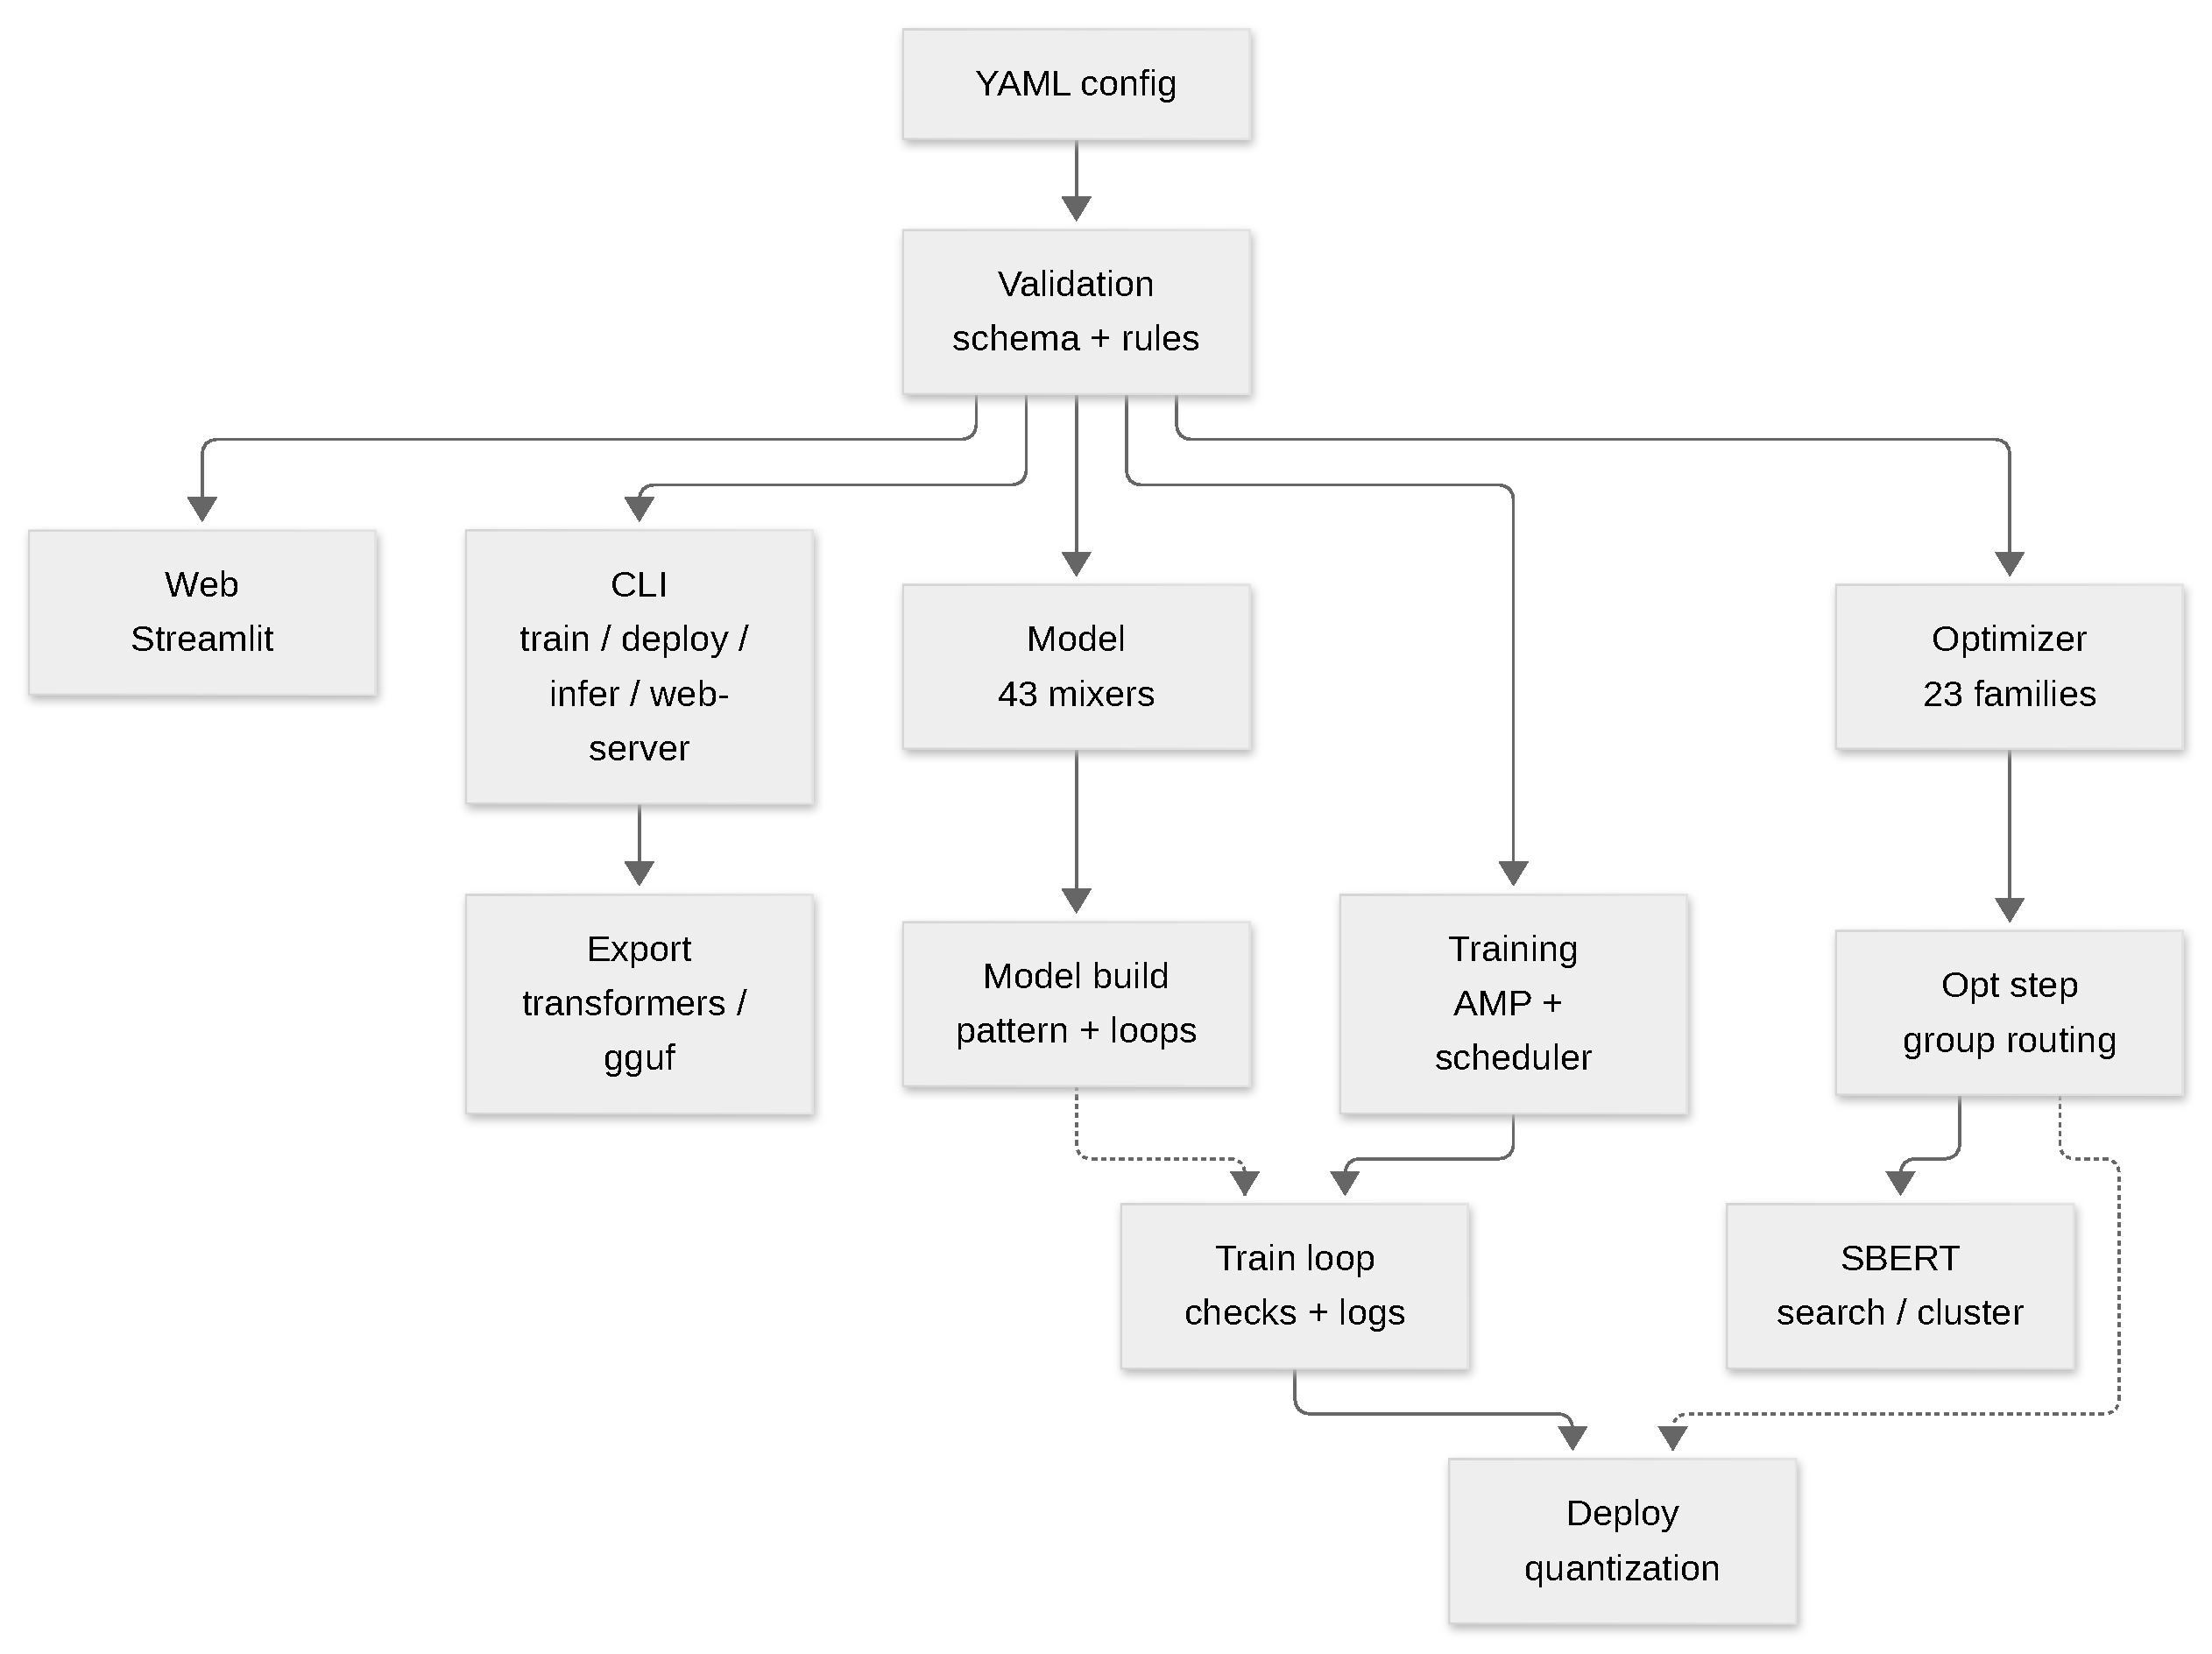
\includegraphics{../paper/figures/system-architecture.pdf}}
\caption{Arquitectura del sistema: la configuración pasa por la validación, se particiona en componentes de modelo, entrenamiento y optimizador, se ejecuta en runtime y produce artefactos de despliegue y SBERT.}
\label{fig:system-architecture}
\end{figure}

\subsection{Alcance del Esquema y Reglas de Validación}
\label{sec:schema-validation}

Los objetos de primer nivel y anidados fijan \texttt{additionalProperties: false}, de modo que las claves desconocidas fallan de inmediato en lugar de ignorarse silenciosamente. Los parámetros del optimizador se restringen además mediante reglas de prefijo por familia. La validación entre componentes rechaza combinaciones incompatibles antes del entrenamiento: el tamaño oculto debe ser divisible por el número de cabezas, el número de cabezas clave--valor debe dividir el número de cabezas, el tamaño del vocabulario debe coincidir con el tokenizer, un modelo base requiere una tarea y (para MLM) un tokenizer, cada tarea requiere su bloque de optimizador correspondiente, las banderas de routers de BitNet requieren BitNet habilitado, y las clases decoder y de visión fuerzan sus respectivos modos de enmascaramiento.

\subsection{Esquema de Configuración}
El esquema completo---campos, tipos, rangos y reglas de validación---se documenta en el Apéndice~\ref{sec:annex-schema}. Los bloques en bucle se configuran con \texttt{num\_layers} y \texttt{num\_loops}, lo que da \texttt{num\_layers}$\times$\texttt{num\_loops} capas lógicas con un conteo de parámetros fijo.

\subsection{Tareas de Entrenamiento}

\texttt{training.task} selecciona el objetivo: \texttt{mlm} (masked language modeling), \texttt{causal\_lm} (predicción autorregresiva de siguiente token, solo clase decoder), \texttt{sbert} (embeddings de oraciones), \texttt{text\_classification} (solo clase encoder) y las tareas de visión \texttt{patch\_prediction}, \texttt{classification} y \texttt{segmentation} (solo Vision Transformer). Las tareas de NLP consumen \texttt{text\_dataset}; las de visión consumen \texttt{vision\_dataset}. Los flujos de embeddings de oraciones se describen en la Sección~\ref{sec:sbert}.

\subsection{Seguridad de Entrenamiento y Semántica de Runtime}

El paso de entrenamiento acumula gradientes sobre micro-lotes, recorta la norma global, verifica desbordamientos posteriores al recorte, reintenta un número acotado de veces ante valores no finitos, despacha el scheduler configurado y rota checkpoints rodantes y del mejor modelo. Cuando \texttt{training.test\_percentage} es positivo, una fracción determinista del dataset se reserva antes del entrenamiento y los pesos finales se evalúan sobre ella; la pérdida y la precisión de la tarea (tasa de error de caracteres para ASR) se escriben en \texttt{test\_metrics.json}. El pseudocódigo completo y la formulación de la partición se remiten al Apéndice~\ref{sec:annex-norm-bitnet-mod}.

\subsection{Variantes de Normalización}
\label{sec:normalization}

La normalización es a la vez una decisión de modelado y una cuestión de compatibilidad del esquema. Los valores aceptados de \texttt{norm.type} son \texttt{layer\_norm}, \texttt{dynamic\_tanh}, \texttt{derf}, \texttt{rms\_norm}, \texttt{prms\_norm} (RMSNorm parcial) y \texttt{flash\_norm} (RMSNorm sin pesos). Sus formulaciones y comparación se detallan en el Apéndice~\ref{sec:annex-norm-bitnet-mod}.

\subsection{Arquitecturas de Flujo Residual}
\label{sec:residual-stream}

Las conexiones residuales se exponen como una decisión de macro-diseño mediante el bloque \texttt{model.residuals}:
\begin{itemize}[leftmargin=*]
    \item \textbf{Estándar}: el residual de identidad clásico \citep{he_deep_2016}.
    \item \textbf{Ninguno}: sin conexión de salto, conservado solo como sonda de ablación.
    \item \textbf{Attention Residuals} (\texttt{full\_attn} o \texttt{block\_attn}): atención aprendida sobre la profundidad que reemplaza la suma residual fija, ya sea sobre todas las capas anteriores o sobre resúmenes por bloques \citep{sun_attnres_2026}.
    \item \textbf{Hiper-conexiones con restricción de variedad} (\texttt{mhc.enabled}): un residual de $n$ flujos cuya matriz de mezcla se restringe al politopo de Birkhoff \citep{xie_mhc_2025}.
\end{itemize}

Attention Residuals se compone con mHC y Mixture-of-Depths; las formulaciones, el cableado y los resultados reportados se recopilan en los Apéndices~\ref{sec:annex-attnres} y~\ref{sec:annex-mhc}.

\section{Taxonomía de Arquitecturas e Implementación}
\label{sec:architecture-taxonomy}

\subsection{Familias de Atención y Mezcladores de Secuencia}
\label{sec:attention-families}

El sistema implementa cuarenta y cuatro mezcladores de secuencia organizados en ocho categorías funcionales que reflejan cómo cada método equilibra expresividad, costo computacional y memoria.
\begin{enumerate}[leftmargin=*]
    \item \textbf{Líneas base densas} (3): atención softmax estándar, atención sigmoide y Grouped-Query Attention (GQA) ofrecen enrutamiento global completo a costo cuadrático.
    \item \textbf{Recurrentes y retentivas} (5): RetNet, Mamba, bloques tipo ODE y Titans mantienen estado para inferencia en tiempo constante mediante recurrencia, espacios de estados selectivos, profundidad continua o memoria en tiempo de prueba.
    \item \textbf{Patrones dispersos} (10): Sparse Transformer, Longformer, SWA con sumideros de atención, BigBird, SparseK, NSA, SpargeAttn, FASA, MSA y SparDA reducen el costo cuadrático mediante dispersión estructurada, selección de tokens o poda sin entrenamiento.
    \item \textbf{Mecanismos con compuerta} (8): GLA, DeltaNet, Gated DeltaNet, Gated DeltaNet-2, HGRN2, FoX, Gated Softmax y KDA introducen control dependiente de los datos sobre retención, olvido y fuerza de actualización.
    \item \textbf{Compresión latente} (10): MLA, GQLA, MLRA, Tucker, IHA, GTA, MTLA, CCA, CCGQA y GMA comprimen el estado clave--valor en cuellos de botella de bajo rango o enrutan mediante una memoria latente de mezcla gaussiana.
    \item \textbf{Memoria condicional} (1): Engram proporciona memoria de lectura/escritura en tiempo de prueba mediante búsquedas aprendidas.
    \item \textbf{Atención de peso rápido} (6): Falcon-1/2/3 y Falcon-1A/2A/3A tratan la transición de estado recurrente como una regla de aprendizaje continuo en línea \citep{zhang_falcon_2026}.
    \item \textbf{Campo geométrico} (1): SSOG aplica un prior geométrico estructurado sobre la matriz de atención \citep{pisoni_ssog_2026}.
\end{enumerate}

\begin{figure}[t]
\centering
\fitfigure{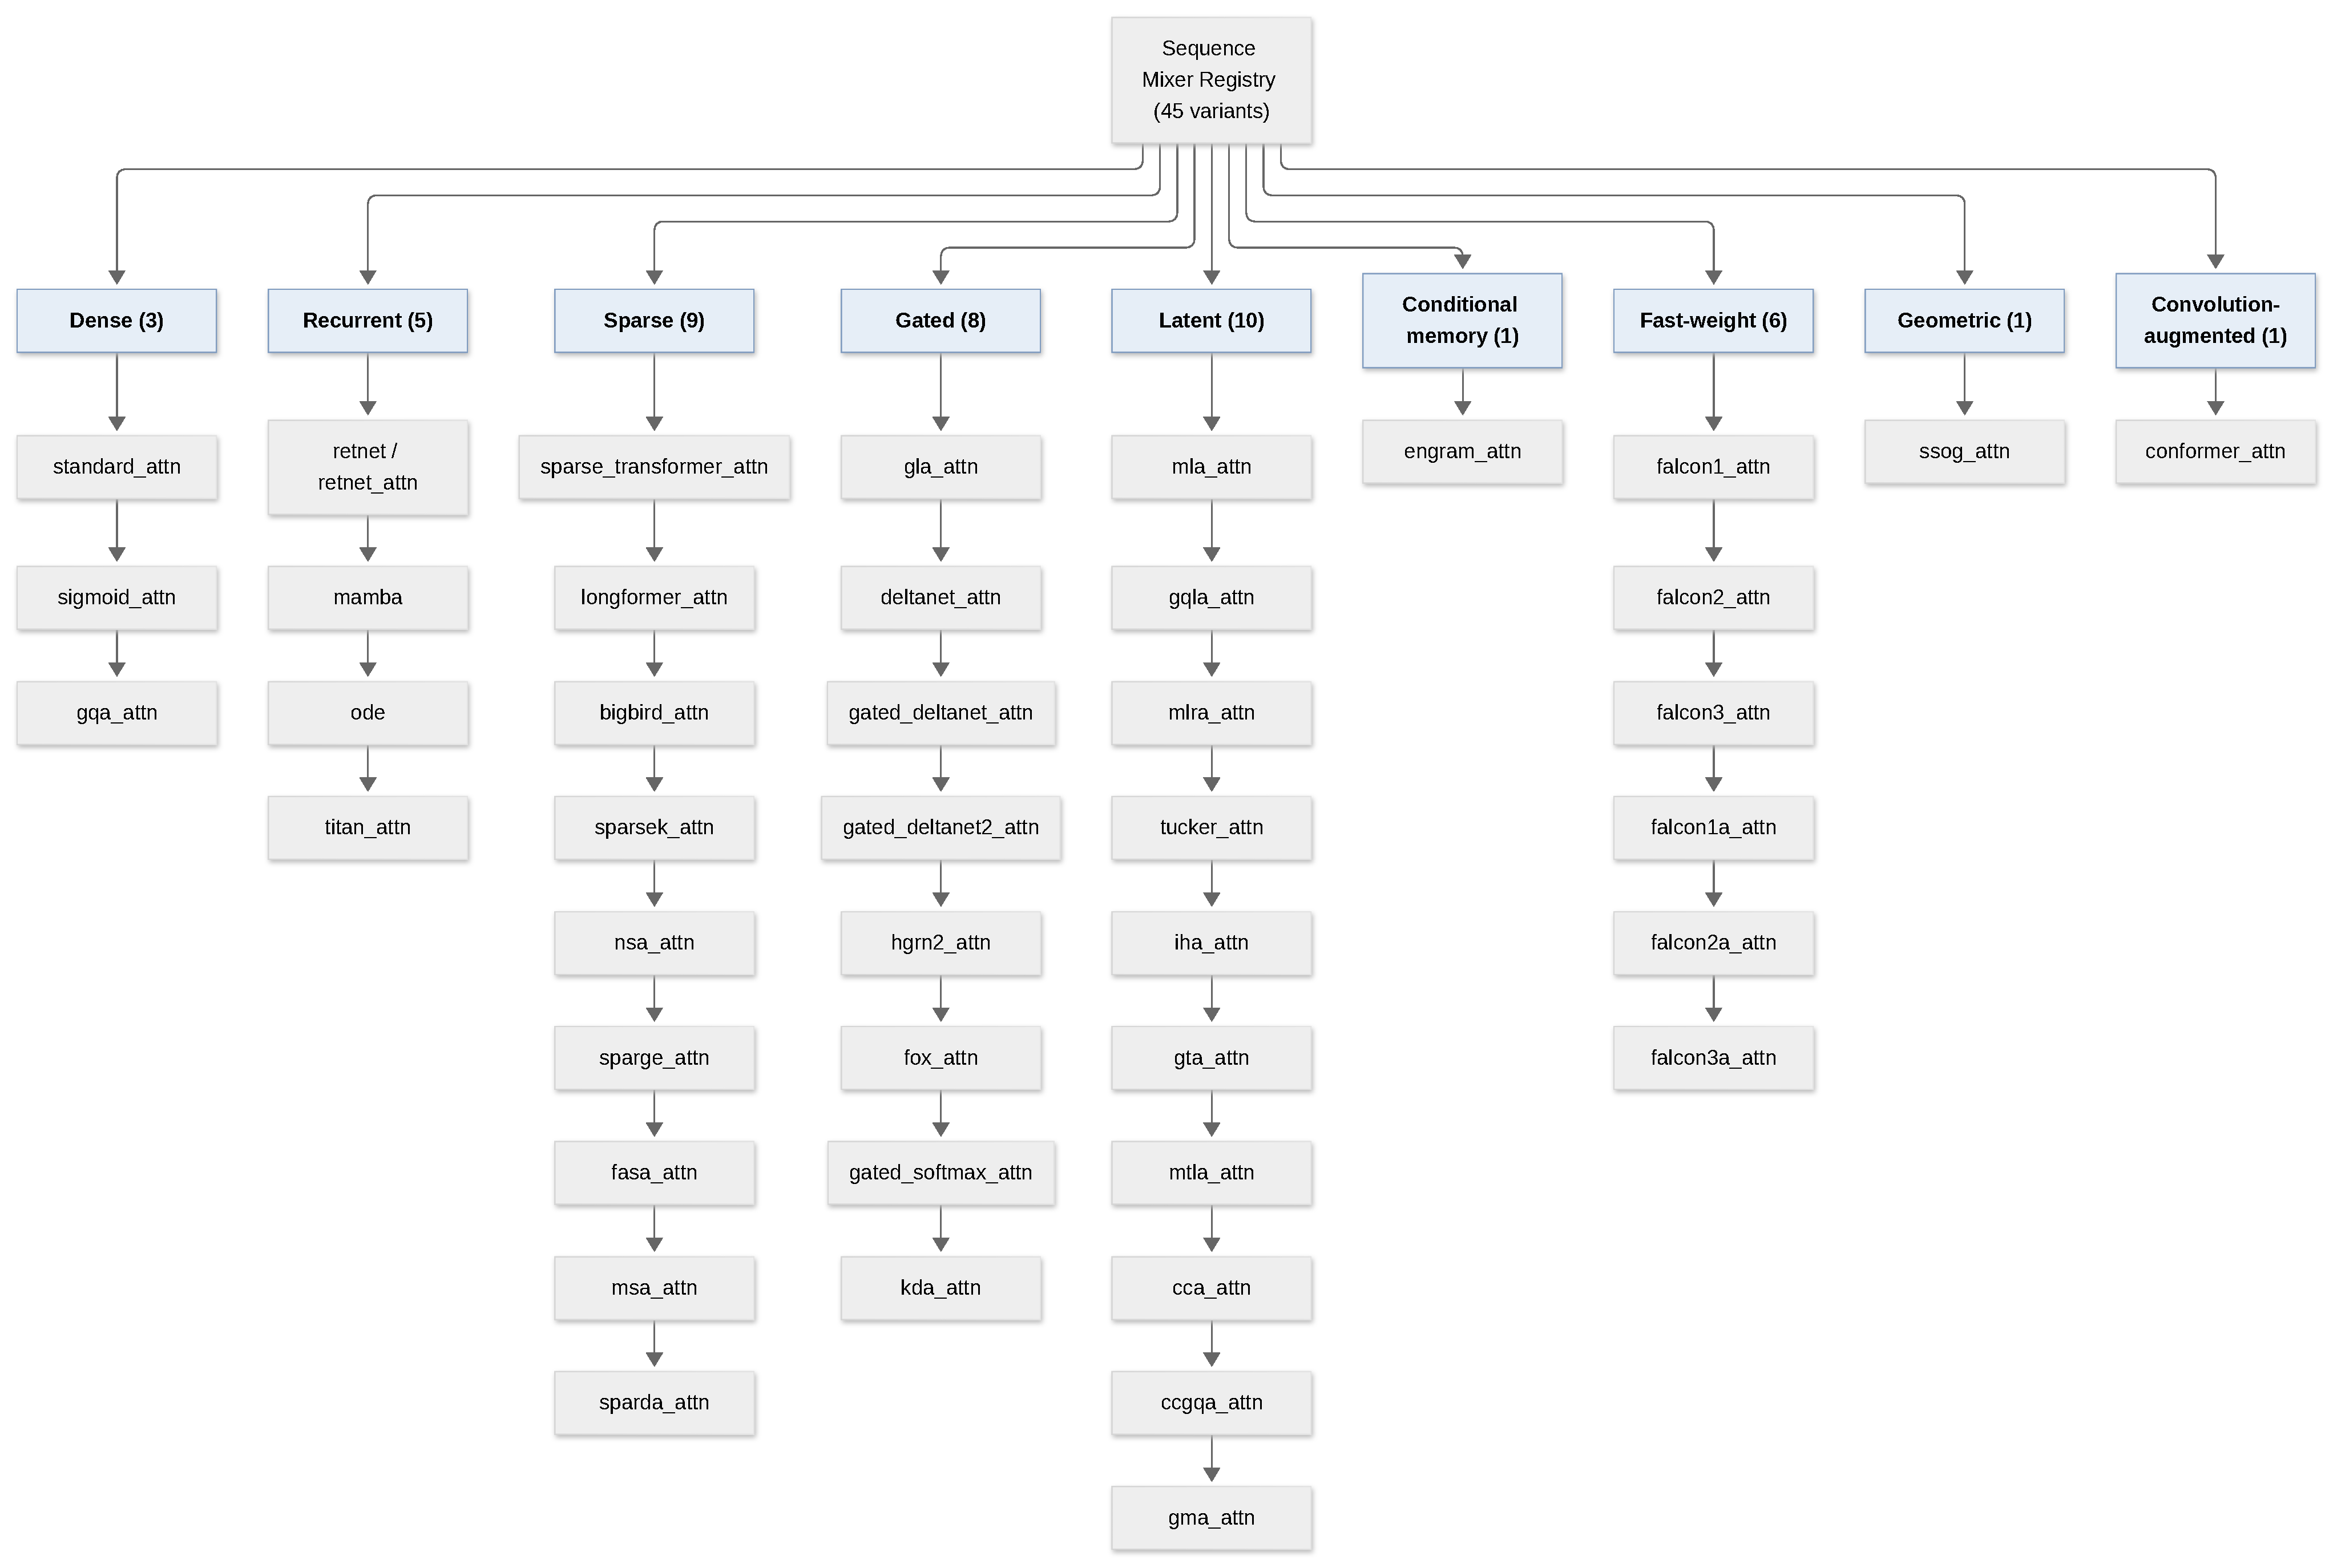
\includegraphics{../paper/figures/mixer-taxonomy.pdf}}
\caption{Taxonomía de los cuarenta y tres mezcladores de secuencia en ocho categorías funcionales. Las líneas base densas ofrecen enrutamiento global completo a costo cuadrático; los métodos recurrentes comprimen el estado para inferencia en tiempo constante; las variantes dispersas restringen el patrón de atención; los mecanismos con compuerta modulan retención y olvido; los métodos latentes comprimen las representaciones clave--valor; la memoria condicional añade búsquedas de lectura/escritura en tiempo de prueba; los métodos de peso rápido formulan la transición de estado como una regla de aprendizaje en línea; los métodos geométricos codifican priors estructurados.}
\label{fig:comprehensive-taxonomy}
\end{figure}

\subsection{Familias Densa y Recurrente}
Las líneas base densas---softmax estándar \citep{vaswani_attention_2017} y atención sigmoide \citep{ramapuram_theory_2024}---y la familia recurrente---RetNet \citep{sun_retentive_2023}, Mamba \citep{gu_mamba_2023}, bloques tipo ODE \citep{zhang_continuous_2021} y Titans \citep{behrouz_titans_2025}---definen el compromiso entre expresividad y eficiencia. Las formulaciones, las formas paralela y recurrente, el pseudocódigo y una tabla comparativa se recopilan en el Apéndice~\ref{sec:annex-transformer}.

\begin{figure}[t]
\centering
\fitfigure{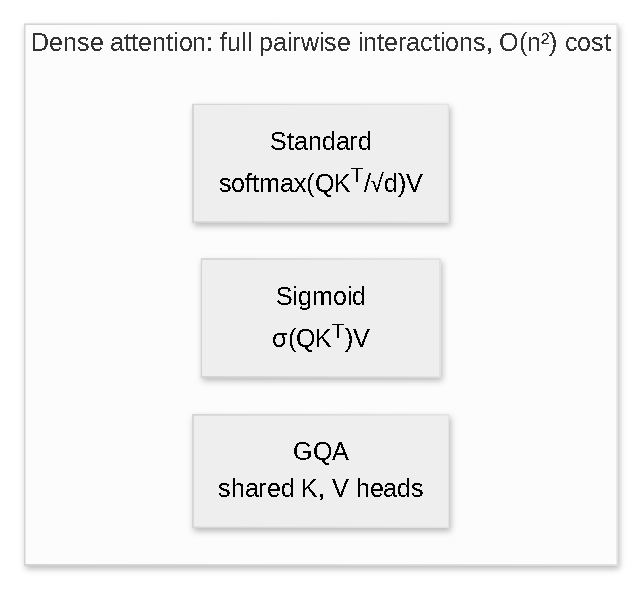
\includegraphics{../paper/figures/dense-map.pdf}}
\caption{Líneas base de atención densa. La atención estándar y la sigmoide calculan interacciones por pares completas; Grouped-Query Attention comparte cabezas clave--valor entre grupos de consultas, reduciendo el tráfico de memoria sin perder la expresividad de la atención completa.}
\label{fig:dense-map}
\end{figure}

\begin{figure}[t]
\centering
\fitfigure{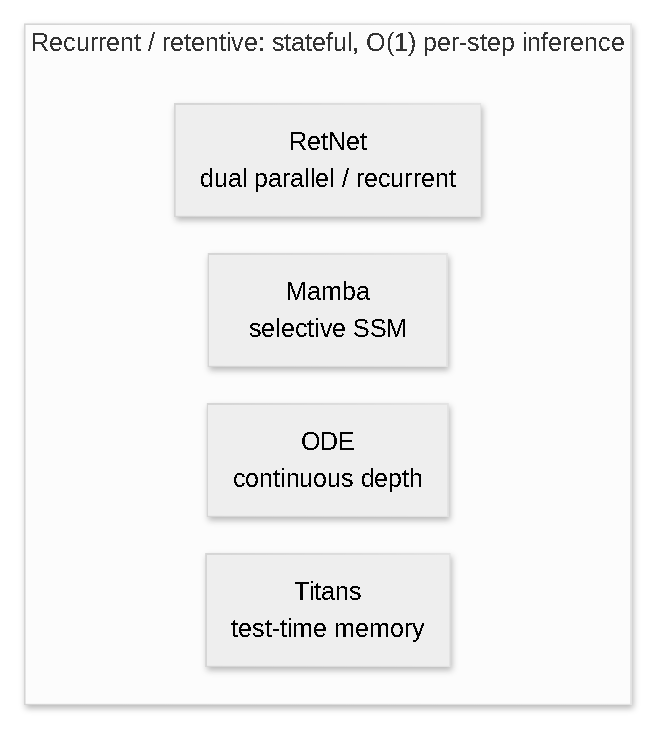
\includegraphics{../paper/figures/recurrent-map.pdf}}
\caption{Familia recurrente y retentiva. RetNet ofrece formas paralela y recurrente, Mamba usa parámetros selectivos de espacio de estados, los bloques ODE modelan profundidad continua y Titans añaden memoria en tiempo de prueba; todos logran inferencia en tiempo constante por paso.}
\label{fig:recurrent-map}
\end{figure}

\subsection{Familia de Atención Latente y de Bajo Rango}
Esta familia comprime el estado clave--valor por token en un latente de bajo rango: MLA, GQLA, MLRA, Tucker, IHA, GTA y MTLA unifican diseños agrupados, latentes, factorizados y temporales. CCA y CCGQA formulan la atención en un latente comprimido con agrupamiento desacoplado, mientras que GMA reemplaza la interacción por pares con enrutamiento probabilístico mediante componentes de mezcla gaussiana aprendidos. Las formulaciones, el pseudocódigo y una tabla comparativa se recopilan en el Apéndice~\ref{sec:annex-latent}.

\begin{figure}[t]
\centering
\fitfigure{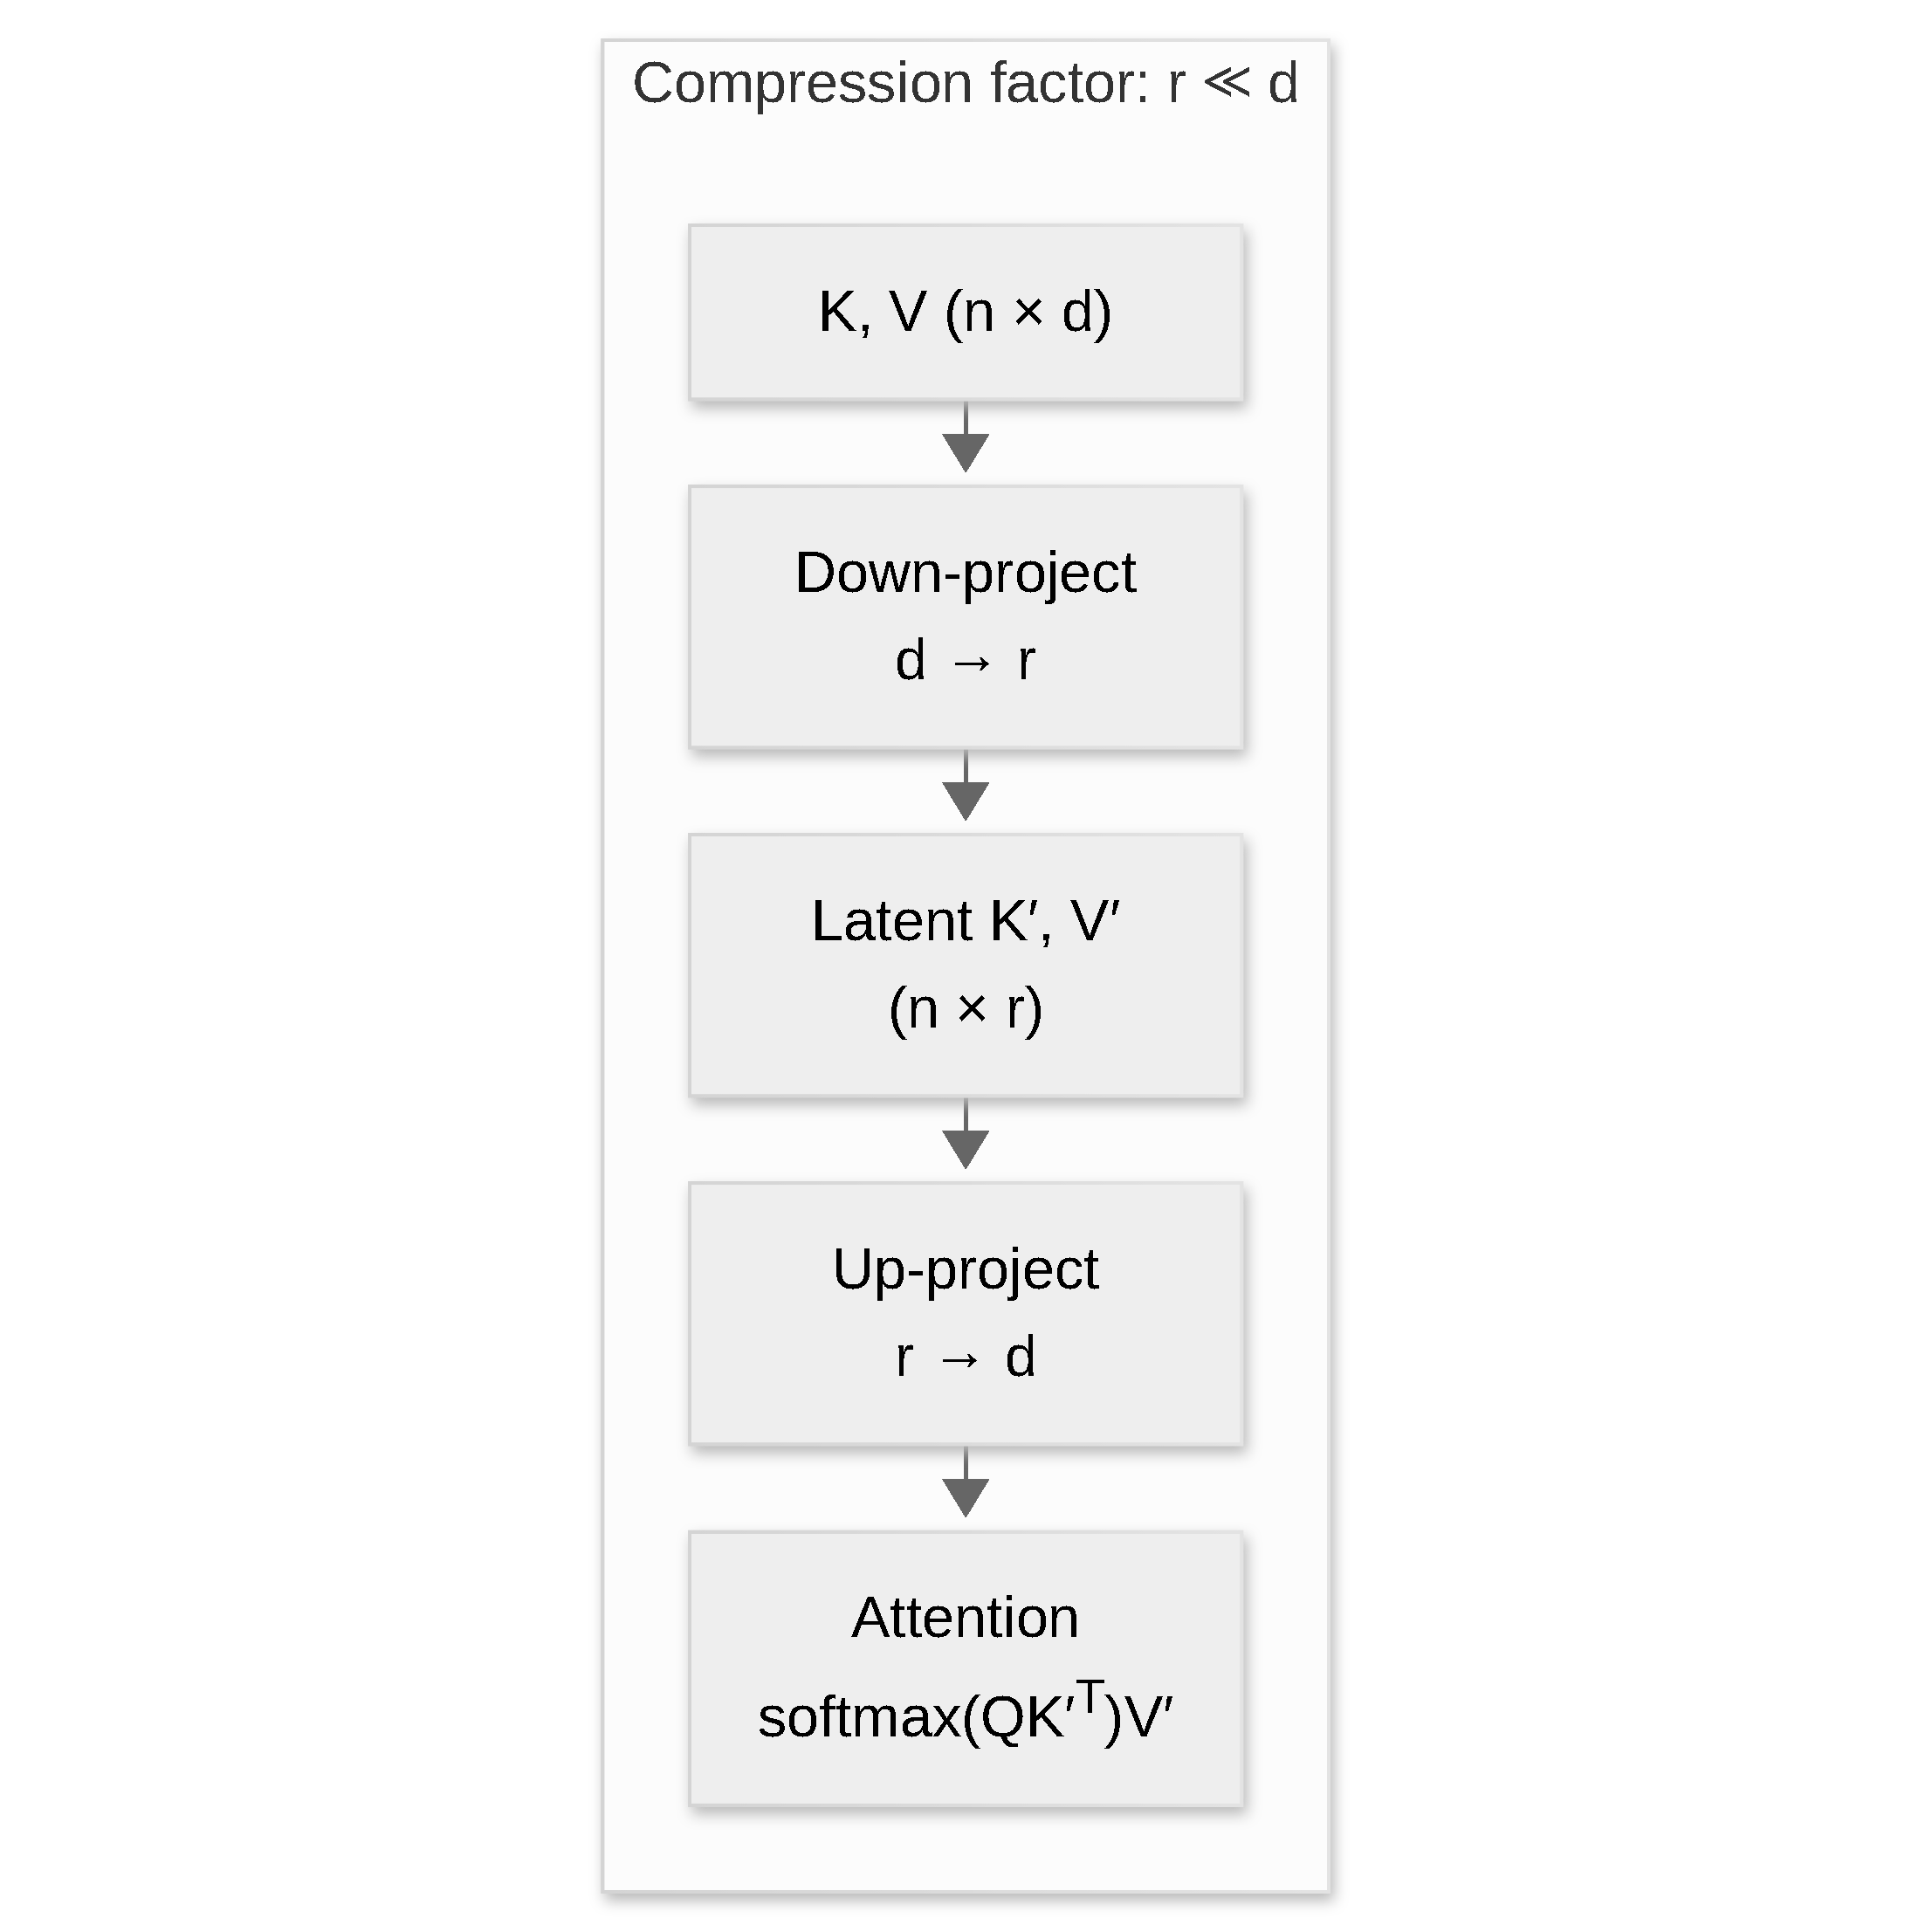
\includegraphics{../paper/figures/latent-map.pdf}}
\caption{Atención latente y de bajo rango. Los pares clave--valor se proyectan a un espacio latente de bajo rango, donde la atención se calcula a menor costo, y se proyectan de vuelta. Las variantes difieren en factorización, intercalado de cabezas, compresión temporal, formulación de covarianza cruzada y enrutamiento probabilístico.}
\label{fig:latent-map}
\end{figure}

\subsection{Extensiones de Atención Dispersa}
El registro incluye diez bloques dispersos \citep{child_sparse_transformer_2019,beltagy_longformer_2020,jolicoeur_sliding_window_2026,zaheer_bigbird_2020,lou_sparsek_2024,yuan_nsa_2025,zhang_spargeattn_2025,wang_fasa_2026,lai_minimax_2026,fu_sparda_2026}. Dos métodos sin entrenamiento, \texttt{fasa\_attn} y \texttt{sparge\_attn}, son solo de evaluación y lanzan un error si se usan durante el entrenamiento; \texttt{swa\_attn} también es sin entrenamiento pero es un mixer entrenable normal, por lo que funciona tanto en entrenamiento como en inferencia. Las formulaciones, el pseudocódigo, las características por bloque y una tabla comparativa se recopilan en el Apéndice~\ref{sec:annex-sparse}.

\begin{figure}[t]
\centering
\fitfigure{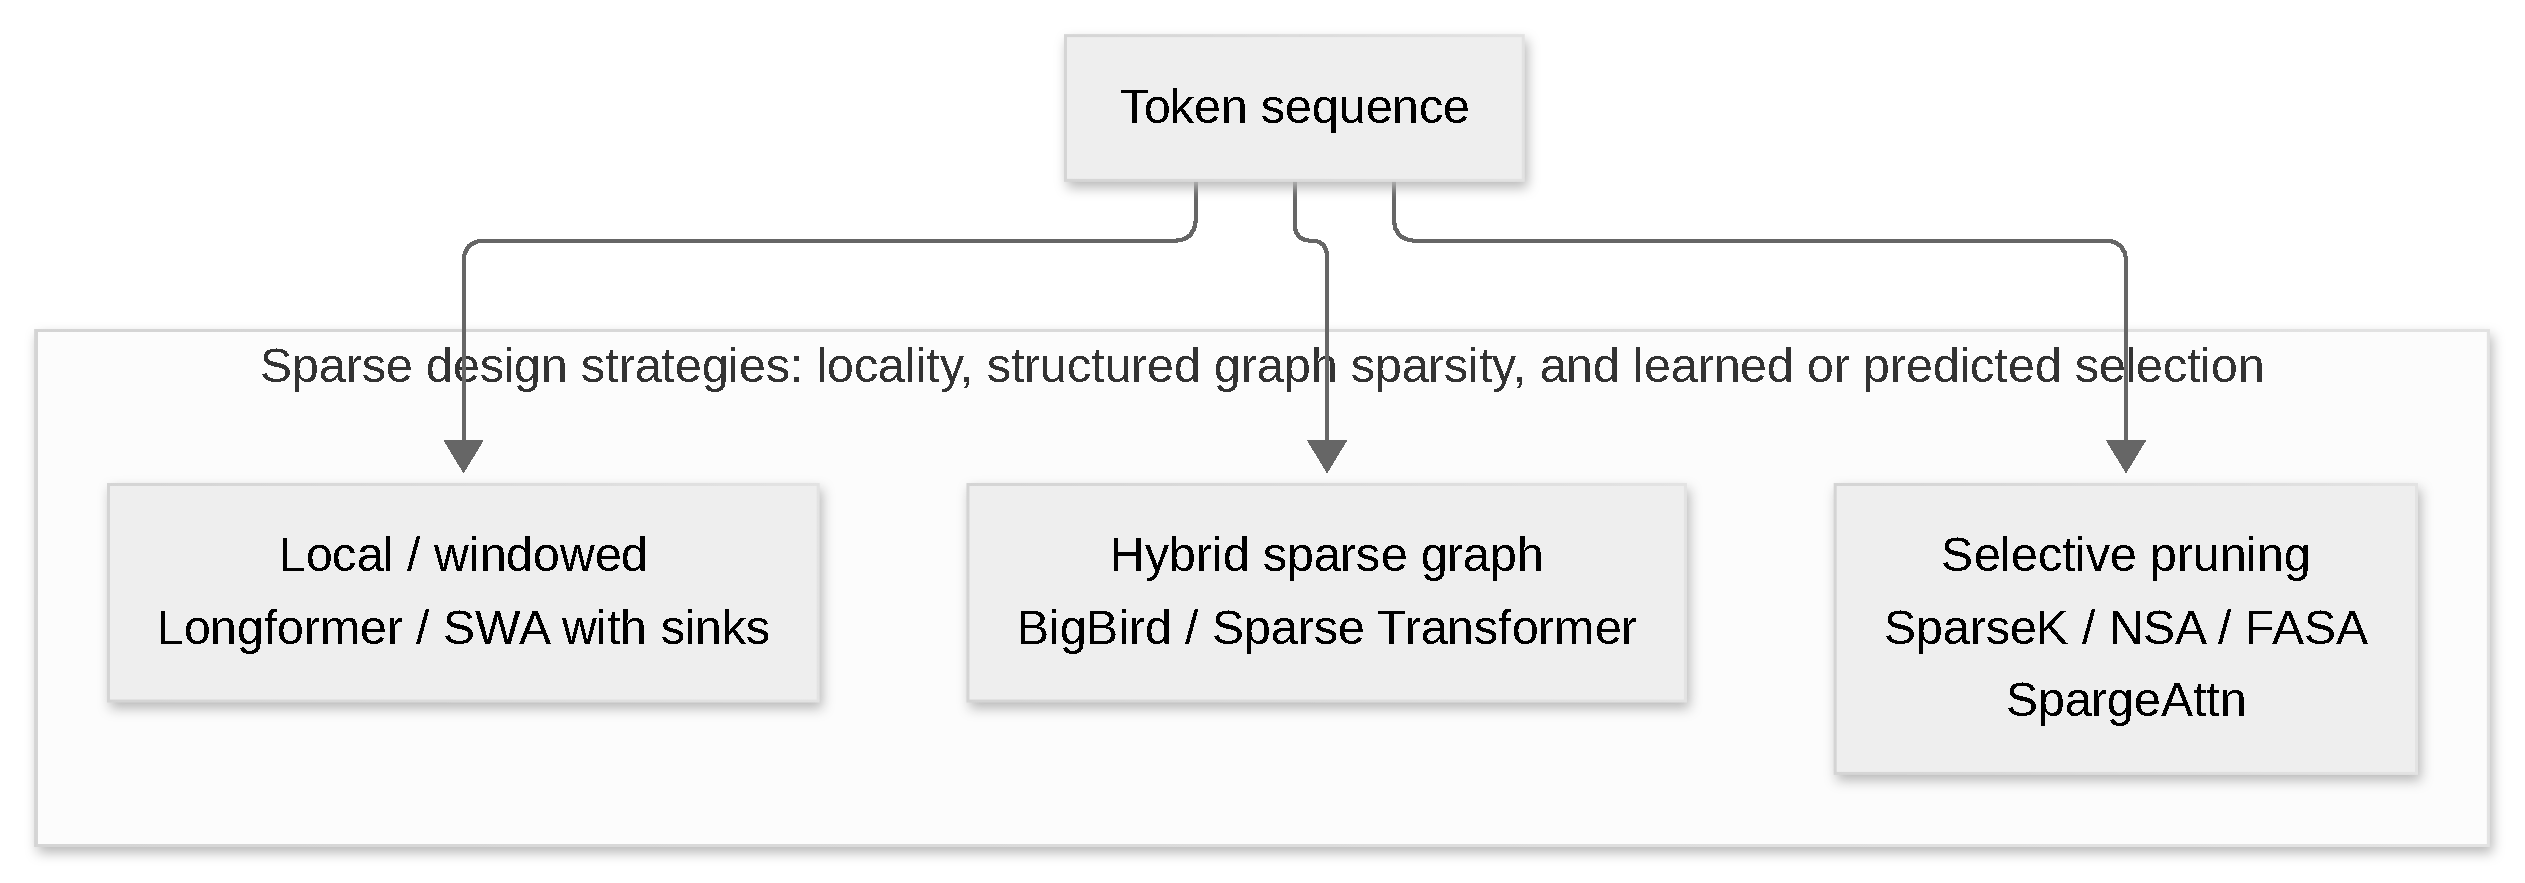
\includegraphics{../paper/figures/sparse-map.pdf}}
\caption{Decisiones de diseño en atención dispersa. Los métodos reducen el costo restringiendo vecindarios, construyendo grafos dispersos o seleccionando solo tokens o bloques de alto valor.}
\label{fig:sparse-map}
\end{figure}

\subsection{Atención con Compuerta y de Peso Rápido}
La familia con compuerta contiene ocho bloques \citep{yang_gla_2023,yang_deltanet_2024,yang_gated_deltanet_2024,hatamizadeh_gated_deltanet2_2026,qin_hgrn2_2024,lin_forgetting_transformer_2025,qiu_gated_attention_2025,kimi_kda_2025}. La compuerta controla qué información sobrevive, ya sea en las actualizaciones de estado recurrente (GLA, variantes de DeltaNet, HGRN2, KDA) o en la ruta de atención completa (FoX, Gated Softmax). Las formulaciones, el pseudocódigo y una tabla comparativa se recopilan en el Apéndice~\ref{sec:annex-gated}.

La atención de peso rápido reformula la actualización recurrente como una regla de aprendizaje continuo en línea; las seis variantes Falcon \citep{zhang_falcon_2026} unifican la regresión estilo DeltaNet y las escrituras de atención lineal bajo semántica de lectura-tras-escritura con tamaños de paso normalizados y olvido explícito. Cada variante incluye un escaneo recurrente de referencia y un kernel paralelo por fragmentos. Las formulaciones, los parámetros de configuración y los resultados publicados se recopilan en el Apéndice~\ref{sec:annex-fast-weight}.

\begin{figure}[t]
\centering
\fitfigure{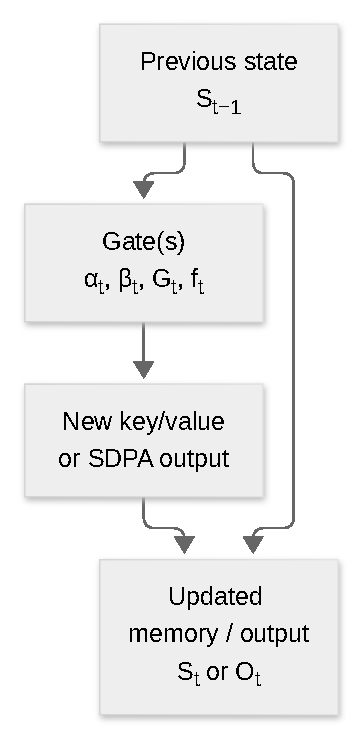
\includegraphics{../paper/figures/gating-template.pdf}}
\caption{Plantilla genérica de compuerta. Una compuerta puede decaer la memoria existente, regular la fuerza de escritura o modular las salidas de atención densa, según la familia de bloques.}
\label{fig:gating-template}
\end{figure}

\section{Familias de Optimizadores y Dinámicas de Entrenamiento}
\label{sec:optimizer-families}

Optimizar arquitecturas transformer grandes se complica por paisajes no convexos, puntos de silla y grupos de parámetros heterogéneos. El sistema soporta veinticuatro familias de optimizadores en siete categorías: líneas base clásicas (SGD con momentum, AdamW, RAdam); momentum y reducción de varianza (Adan, ADOPT, AdEMAMix, MARS, Cautious AdamW); métodos eficientes en memoria y de bajo rango (Adafactor, GaLore, Lion, APOLLO, APOLLO-Mini, Q-APOLLO); métodos sin programación y sin parámetros (Schedule-Free AdamW, Prodigy) con escalado para lotes grandes (LAMB); métodos conscientes de la curvatura y de segundo orden (Sophia, Shampoo, SOAP); métodos orientados a geometría (Muon, Turbo-Muon, AF-Muon); y optimizadores de adaptividad ajustable (Anon). Los algoritmos, el pseudocódigo y las comparaciones de memoria y complejidad se recopilan en el Apéndice~\ref{sec:annex-optimizers}.

\begin{figure}[t]
\centering
\fitfigure{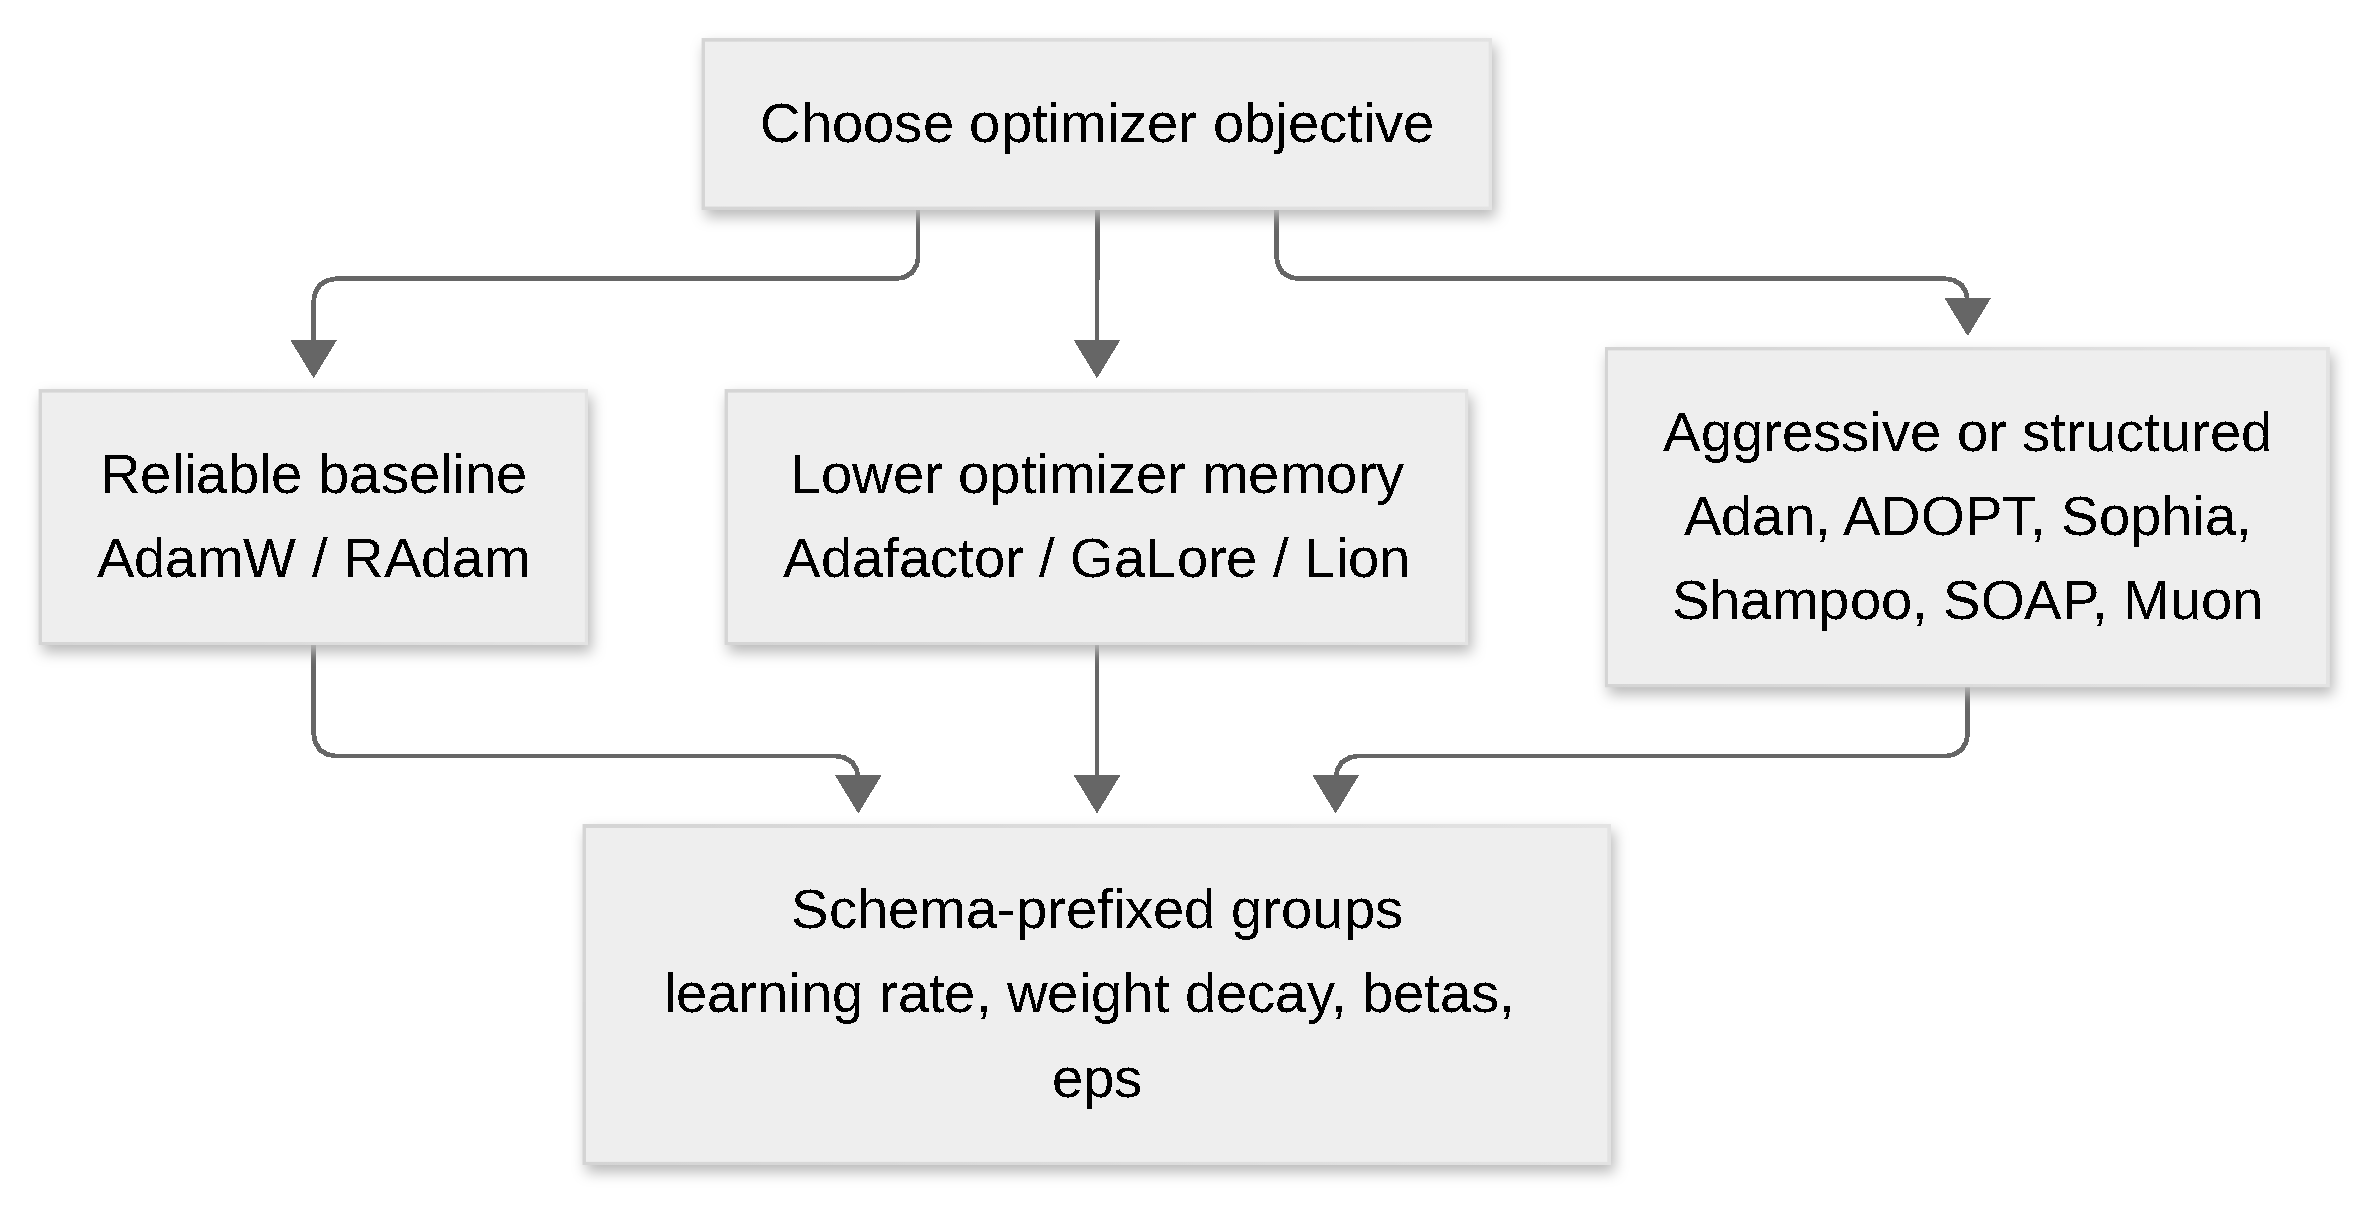
\includegraphics{../paper/figures/optimizer-routing.pdf}}
\caption{Selección de optimizador en la práctica: la clase determina la regla de actualización, mientras que el esquema controla cómo se aplican los hiperparámetros en los diez bloques canónicos de parámetros (embeddings, encodings posicionales, atención, feed-forward, normalización, heads, mHC, routers, residuales y el resto de parámetros).}
\label{fig:optimizer-routing}
\end{figure}

\section{Cuantización y Despliegue}
\label{sec:quantization}

La etapa de despliegue convierte un checkpoint entrenado en un artefacto compacto mediante empaquetado ternario de pesos \citep{wang_bitnet_2023} y escalado de activaciones INT8, con estimaciones de tamaño alineadas con objetivos de despliegue ligero \citep{samson_lightweight_2026,bravin_embbert_2026}. El mismo subcomando emite artefactos estándar o cuantizados, o exporta formatos HuggingFace Transformers y BitNet GGUF para runtimes externos. Las formulaciones y las estimaciones de tamaño se remiten al Apéndice~\ref{sec:annex-norm-bitnet-mod}.

\begin{figure}[t]
\centering
\fitfigure{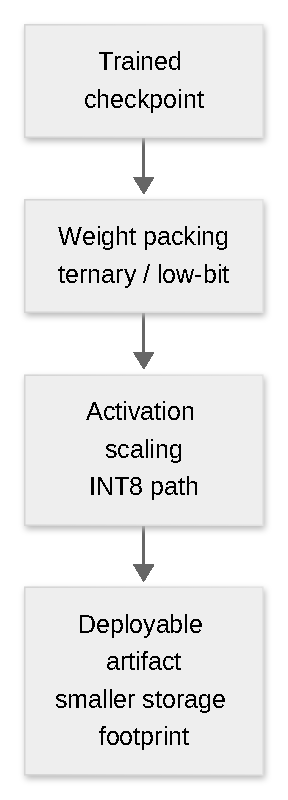
\includegraphics{../paper/figures/deploy-flow.pdf}}
\caption{Ruta de despliegue desde un checkpoint entrenado hasta un artefacto compacto. La cuantización es una transformación de la etapa de despliegue, no una familia de modelos separada.}
\label{fig:deploy-flow}
\end{figure}

\section{Tareas Posteriores de SBERT}
\label{sec:sbert}

El embedding de oraciones se construye sobre entrenamiento estilo Siamese \citep{reimers_sentence-bert_2019}. Para el par de oraciones $(s_1,s_2)$ con embeddings $(e_1,e_2)$:
\[
\text{cos}(e_1,e_2)=\frac{e_1^\top e_2}{\|e_1\|\|e_2\|}
\]
y pérdida coseno estilo regresión:
\[
\mathcal{L}_{\text{cos}}=\left(\text{cos}(e_1,e_2)-y\right)^2
\]
con $y\in[-1,1]$ en este pipeline.

Modos posteriores soportados:
\begin{itemize}[leftmargin=*]
    \item \textbf{Similitud}: puntuación por pares entre dos oraciones.
    \item \textbf{Búsqueda}: $k$ vecinos más cercanos sobre un corpus.
    \item \textbf{Clustering}: agrupación de embeddings (ej., k-means).
    \item \textbf{Codificación}: exportación persistente de embeddings para recuperación posterior.
\end{itemize}

\begin{figure}[t]
\centering
\fitfigure{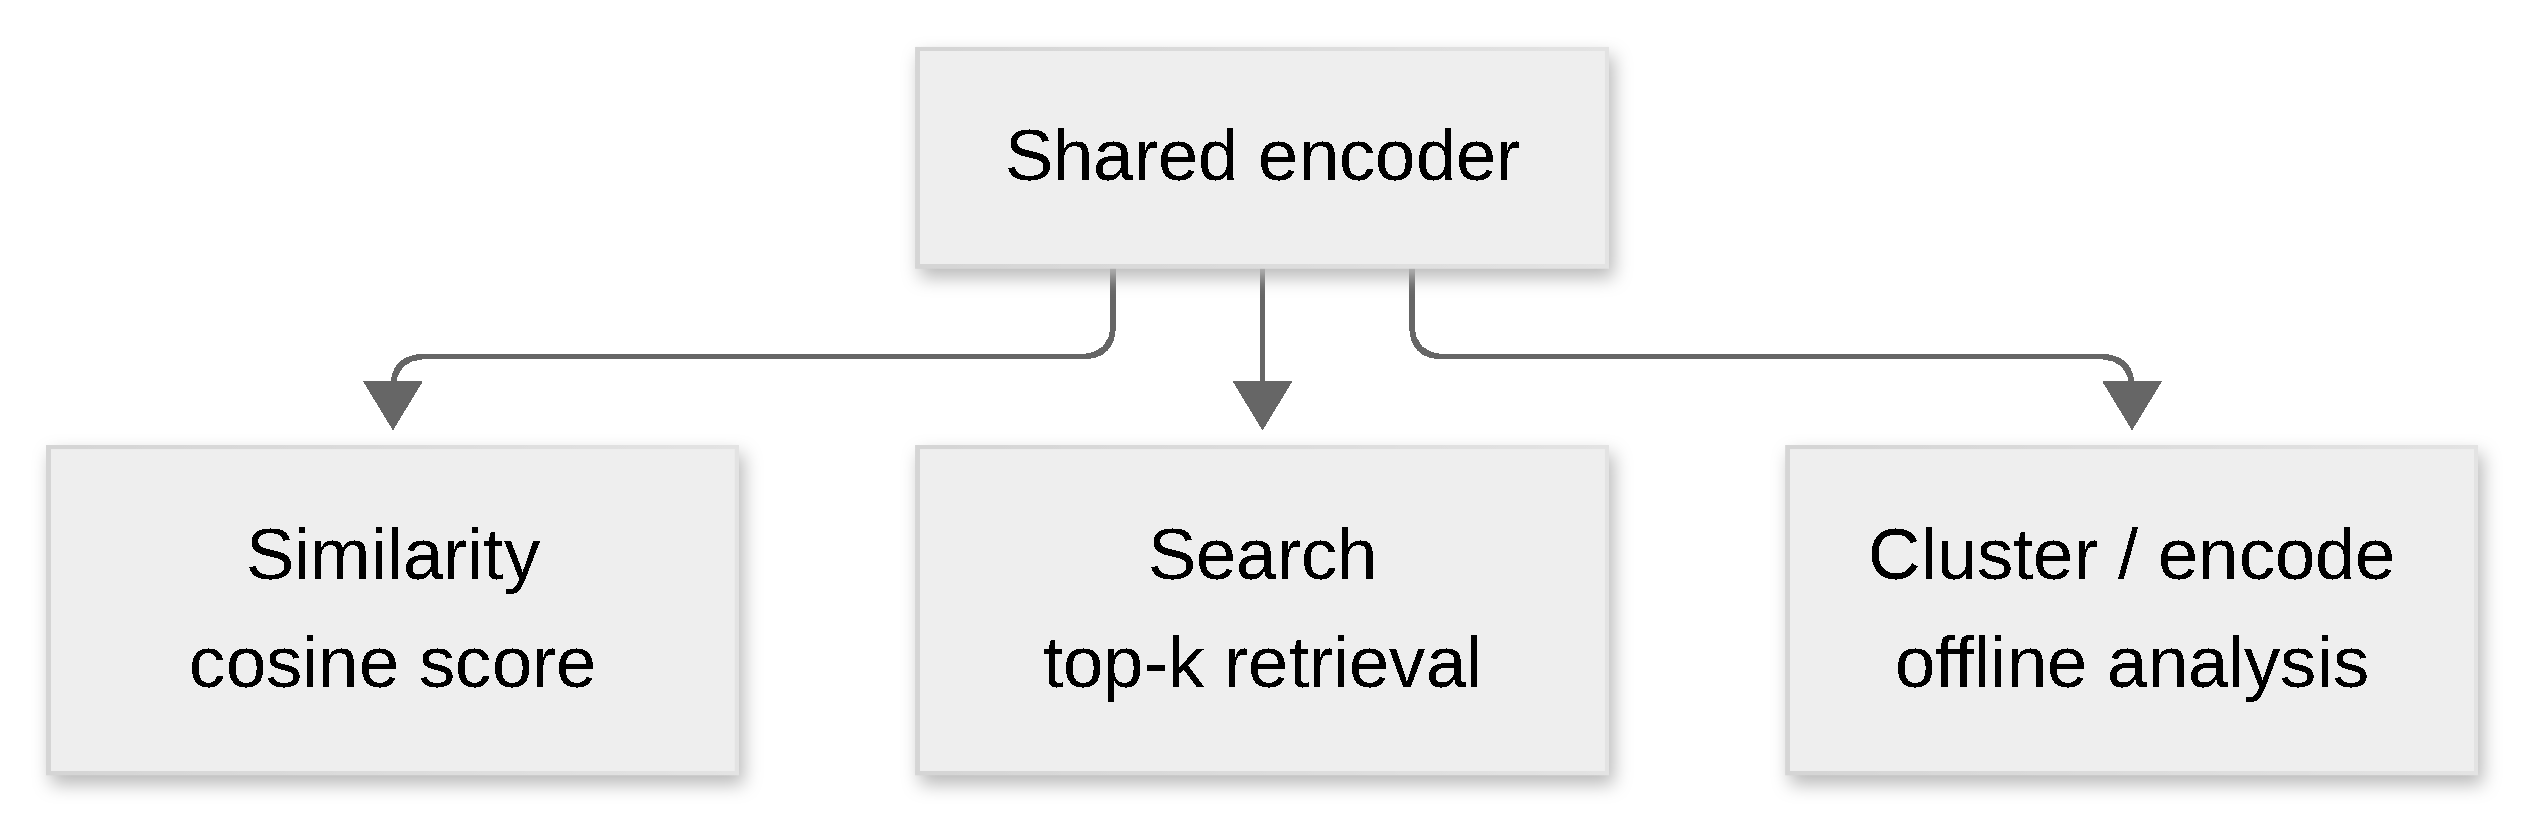
\includegraphics{../paper/figures/sbert-modes.pdf}}
\caption{Reutilización del flujo de trabajo SBERT. Un único codificador soporta puntuación de pares en línea, recuperación sobre corpus, clustering y exportación persistente de embeddings.}
\label{fig:sbert-modes}
\end{figure}

El pseudocódigo del enrutador de modo de inferencia SBERT---despachando entre los modos de similitud, búsqueda, cluster y codificación sobre un codificador compartido---se remite al Apéndice~\ref{sec:annex-norm-bitnet-mod}.


\section{Integración Sin Código: El Plugin \texttt{dashai-frankenstein}}
\label{sec:dashai-plugin}

El CLI y el generador web descritos en la Sección~\ref{sec:system-design} sirven a investigadores cómodos con archivos de configuración YAML. Una audiencia complementaria---especialistas de dominio, educadores y analistas que necesitan un modelo entrenado pero no un script de entrenamiento---está mejor servida por un entorno gráfico. Por ello, Frankenstein Transformer distribuye \texttt{dashai-frankenstein}, un adaptador que registra sus clases de modelo como componentes de \textbf{dashAI} (\texttt{\url{https://github.com/DashAISoftware/dashAI}}), una aplicación de escritorio open-source y local-first para aprendizaje automático desarrollada por un consorcio académico chileno (Universidad de Chile/FCFM, CENIA, IMFD y financiamiento ANID). Ambos sistemas están basados en esquemas---dashAI genera formularios desde esquemas Pydantic y Frankenstein valida YAML contra un JSON Schema estricto---por lo que la integración deja intacto el backend de dashAI; el plugin se descubre mediante el grupo de entry-points estándar \texttt{dashai.plugins} documentado en la guía de plugins de dashAI (\texttt{\url{https://docs.dash-ai.com/learn/guides/plugins/}}).

\subsection{Componentes Registrados}

Un único grupo de entry-points registra cinco componentes:
\begin{itemize}[leftmargin=*]
    \item \textbf{\texttt{FrankensteinMLMModel}} (\texttt{BaseModel}, \texttt{TextClassificationTask}): encoder con una cabeza de clasificación sobre la salida agrupada; \texttt{predict} devuelve probabilidades por clase.
    \item \textbf{\texttt{FrankensteinDecoderModel}} (\texttt{BaseGenerativeModel}, \texttt{TextToTextGenerationTask}): fuerza la clase decoder y expone muestreo autorregresivo top-$k$.
    \item \textbf{\texttt{FrankensteinViTClassifier}} (\texttt{BaseModel}, \texttt{ImageClassificationTask}): usa la cabeza de clasificación del ViT (Apéndice~\ref{sec:annex-vision}).
    \item \textbf{\texttt{FrankensteinViTSegmenter}} (\texttt{BaseModel}, \texttt{SegmentationTask} del plugin): usa la cabeza de segmentación del ViT y devuelve mapas de clases por píxel.
    \item \textbf{\texttt{SegmentationTask}} (\texttt{BaseTask}): declara el contrato imagen-entrada/máscara-salida que dashAI no incluye.
\end{itemize}

Todos comparten una fachada delgada sobre la API del motor, de modo que el plugin tiene una única dependencia pesada.

\subsection{Esquema de Configuración de Passthrough}

El JSON Schema de Frankenstein sigue siendo la única fuente de verdad en lugar de traducir sus campos a formularios nativos de dashAI. Cada componente expone un campo \texttt{frankenstein\_json} que contiene una configuración completa de entrenamiento como JSON de una sola línea. Antes de ejecutar cualquier entrenamiento, el adaptador parsea el JSON, lo valida contra el esquema resuelto y aplica las verificaciones cruzadas del cargador de configuración; los fallos se presentan como un error legible etiquetado con la etapa fallida. Los adaptadores de datasets mapean los datasets de dashAI a las expectativas de Frankenstein, inyectan el tamaño de vocabulario desde el tokenizador resuelto y transmiten las métricas por época a dashAI.

\subsection{Estado}

Las tres fases de implementación---MVP de clasificación, decoder generativo y clasificador ViT, y segmentador ViT---están completas, pero el paquete aún no se ha ejecutado dentro de una instancia viva de dashAI y la publicación en PyPI está pendiente. Las limitaciones conocidas incluyen un bucle de clasificación directo en lugar de preentrenamiento MLM, campos nativos diferidos para ajustes de alto impacto y renderizado no confirmado de máscaras de segmentación. El adaptador deja deliberadamente intacto el núcleo de dashAI, de modo que futuros releases no puedan romperlo por acoplamiento.

\section{Discusión}
\label{sec:discussion}

Las decisiones de diseño en Frankenstein Transformer reflejan varias tensiones de ingeniería e investigación en las herramientas modernas de aprendizaje profundo.

\subsection{Compromisos de Diseño Basado en Esquemas}

El enfoque basado en esquemas proporciona beneficios significativos de reproducibilidad al imponer contratos explícitos y fallar rápidamente ante configuraciones inválidas. Sin embargo, este enfoque también introduce rigidez: agregar nuevas arquitecturas u optimizadores requiere extensiones del esquema en lugar de argumentos de línea de comandos flexibles. El sistema de hiperparámetros prefijados permite un control detallado pero aumenta la complejidad de configuración para usuarios acostumbrados a interfaces más simples.

La decisión de imponer \texttt{additionalProperties: false} en todos los niveles del esquema elimina la absorción silenciosa de parámetros que ha afectado a sistemas de configuración anteriores, pero esta rigurosidad requiere un mantenimiento cuidadoso del esquema al extender las capacidades del sistema. Cada nuevo mecanismo de atención o variante de optimizador debe integrarse adecuadamente en el marco de validación, incluyendo definiciones de campos del esquema con tipos y restricciones apropiados, mapeo de hiperparámetros prefijados para grupos específicos de optimizadores, valores predeterminados alineados con las mejores prácticas de investigación y cadenas de documentación para la representación en la interfaz web.

\subsection{Cobertura Arquitectónica y Vacíos}

Las cuarenta y tres arquitecturas de mezclador implementadas abarcan las principales direcciones de investigación en modelado de secuencias, pero ciertos vacíos permanecen. El sistema carece de arquitecturas híbridas recientes como Griffin \citep{soares_griffin_2024} y Jamba \citep{gu_jamba_2024}, que combinan compuertas con modelos de espacio de estados. El enrutamiento MoE (Mezcla de Expertos) está implementado para capas FFN pero no para el cómputo de atención, donde trabajos recientes han mostrado beneficios \citep{lewis_moe_2021}.

La cobertura de atención dispersa es amplia. Los dos métodos en tiempo de inferencia (FASA, SpargeAttn) conservan su carácter sin entrenamiento en el sentido de que su regla de dispersidad nunca se aprende; en cambio, la implementación entrena la capa como atención estándar densa sobre las mismas proyecciones y activa la ruta de selección/poda dispersa solo en evaluación, de modo que ambos mixers pueden entrenarse desde cero y su comportamiento disperso es exactamente el descrito en los artículos originales.

La cobertura de mecanismos de compuerta y peso rápido abarca las categorías principales, incluidas las seis variantes Falcon \citep{zhang_falcon_2026}. El macro-diseño del flujo residual está cubierto por Attention Residuals \citep{sun_attnres_2026} y por el flujo residual de $n$ streams restringido por variedad (mHC) \citep{xie_mhc_2025}, cuya proyección Sinkhorn--Knopp sobre el politopo de Birkhoff restaura la propiedad de mapeo de identidad que pierden las hiper-conexiones sin restricción; mHC está validado solo al nivel de los experimentos MoE publicados de 3B--27B y se beneficiaría de reproducciones independientes a escalas menores (Apéndice~\ref{sec:annex-mhc}).

\subsection{Fragmentación del Panorama de Optimizadores}

El soporte para veinticuatro familias de optimizadores en siete categorías demuestra exhaustividad pero también resalta el estado fragmentado de la investigación en optimización. Los usuarios enfrentan una complejidad significativa de decisión al elegir entre métodos de reducción de varianza (Adan, MARS), variantes eficientes en memoria (GaLore, Adafactor, APOLLO) y enfoques conscientes de curvatura (Sophia, Shampoo). El sistema de hiperparámetros prefijados, aunque poderoso, requiere comprender qué parámetros son relevantes para cada clase de optimizador.

La calidad de implementación varía entre optimizadores: los métodos clásicos (AdamW, SGD con momento) están altamente optimizados en PyTorch, mientras que los métodos más nuevos (Muon, Turbo-Muon, AF-Muon, SOAP) pueden requerir implementaciones personalizadas que afectan la estabilidad numérica y las características de rendimiento.

\subsection{Consideraciones de Despliegue y Producción}

El pipeline de cuantización demuestra preocupaciones prácticas de despliegue pero realiza compromisos de ingeniería específicos. El empaquetado ternario de pesos reduce el almacenamiento a aproximadamente $1.58$ bits por parámetro, pero esta compresión agresiva puede degradar el rendimiento, especialmente para modelos más pequeños donde el error de cuantización es más significativo. La implementación actual aplica cuantización uniforme entre todos los tipos de parámetros.

Los flujos de trabajo SBERT proporcionan utilidad práctica para tareas de similitud semántica y recuperación, pero la implementación asume estrategias de pooling estándar (token CLS, pooling promedio). Avances recientes como los embeddings Matryoshka \citep{muennighoff_matryoshka_2021} y los refinamientos de aprendizaje contrastivo \citep{chen_supervised_2020} aún no están incorporados.

\subsection{Desafíos de Integración y Extensibilidad}

La estructura actual del código base, aunque funcional, presenta desafíos de mantenimiento a medida que se expanden las familias de arquitecturas y optimizadores. El patrón de despachador para la selección de mezcladores y el enrutamiento de optimizadores maneja la extensibilidad pero corre el riesgo de convertirse en un ``cajón de sastre'' de lógica condicional. Las versiones futuras se beneficiarían de arquitecturas basadas en plugins donde nuevos mezcladores y optimizadores puedan registrarse de forma declarativa en lugar de modificar la lógica central de despacho.

La interfaz de configuración web proporciona mejoras significativas de usabilidad pero introduce complejidad de despliegue: ejecutar Streamlit junto con trabajos de entrenamiento requiere recursos adicionales y consideraciones de infraestructura que pueden no ser apropiadas para todos los entornos, particularmente clústeres HPC sin acceso web.


\section{Conclusión}
\label{sec:conclusion}

Frankenstein Transformer presenta una plataforma de experimentación unificada, impulsada por configuración, que aborda tres desafíos de la investigación moderna en aprendizaje profundo: fragmentación arquitectónica entre atención densa, modelos recurrentes, patrones dispersos, mecanismos de compuerta, compresión latente, memoria condicional, memorias de peso rápido y priors geométricos; complejidad del panorama de optimizadores que abarca líneas base clásicas, métodos de reducción de varianza, variantes eficientes en memoria, enfoques sin programación, algoritmos conscientes de curvatura y métodos orientados a geometría; y flujos de trabajo de despliegue de extremo a extremo que abarcan cuantización y embeddings de oraciones.

Las contribuciones principales del sistema son:
\begin{enumerate}[leftmargin=*]
    \item \textbf{Diseño Basado en Esquemas}: Un contrato de configuración estricto basado en YAML con validación y enrutamiento de hiperparámetros prefijados que permite experimentos reproducibles en cuarenta y tres mezcladores de secuencia y veintitrés familias de optimizadores.
    \item \textbf{Soporte Arquitectónico Integral}: Implementación que abarca líneas base densas, bloques recurrentes y retentivos, atención dispersa, mecanismos con compuerta, compresión latente, memoria condicional, atención de peso rápido y atención de campo geométrico, con clases de modelo encoder, decoder y Vision Transformer.
    \item \textbf{Marco Unificado de Optimizadores}: Grupos de hiperparámetros prefijados que permiten control detallado sobre embeddings, capas de normalización, pesos de atención y el resto de parámetros en líneas base clásicas (SGD+Momentum, AdamW, RAdam), reducción de varianza (Adan, ADOPT, AdEMAMix, MARS, Cautious), métodos eficientes en memoria y de bajo rango (Adafactor, GaLore, Lion, APOLLO, APOLLO-Mini, Q-APOLLO), lotes grandes y simplificación de programación (LAMB, Schedule-Free AdamW, Prodigy), conscientes de curvatura (Sophia), segundo orden (Shampoo, SOAP), orientados a geometría (Muon, Turbo-Muon) y adaptividad ajustable (Anon).
    \item \textbf{Flujos de Trabajo de Extremo a Extremo}: Pipeline de despliegue integrado que soporta empaquetado ternario de pesos y cuantización de activaciones INT8; entrenamiento e inferencia inspirados en SBERT para similitud semántica, recuperación y tareas de clustering.
    \item \textbf{Configuración Interactiva}: Interfaz web basada en Streamlit que proporciona generación de formularios impulsada por esquemas, validación en tiempo real, documentación en línea y síntesis de comandos CLI.
\end{enumerate}

Este sistema permite iteración experimental rápida mientras mantiene reproducibilidad mediante contratos de configuración estrictos. Al consolidar diversas contribuciones de investigación en un conjunto de herramientas unificado, reduce las barreras para explorar arquitecturas y estrategias de optimización novedosas, particularmente para investigadores que pueden carecer de recursos para implementar y validar cada variante de forma independiente.

\subsection{Limitaciones y Direcciones Futuras}

Varias limitaciones y direcciones prometedoras para trabajo futuro surgen del diseño e implementación de este sistema:

\begin{enumerate}[leftmargin=*]
    \item \textbf{Integración Arquitectónica}: Arquitecturas híbridas recientes (Griffin, Jamba, Mamba-X) demuestran beneficios de combinar múltiples mecanismos en bloques unificados. Versiones futuras deberían integrar estas arquitecturas y explorar patrones de composición sistemática.
    
    \item \textbf{Cuantización Avanzada}: La implementación actual utiliza empaquetado ternario uniforme en todos los parámetros. La investigación sobre cuantización por capas, por canales y consciente de importancia sugiere que estrategias más sofisticadas podrían mejorar los compromisos calidad-eficiencia.
    
    \item \textbf{Extensibilidad Basada en Plugins}: El patrón de despacho actual se vuelve cada vez más complejo con cada nueva adición. Una arquitectura de plugins que permita el registro declarativo de nuevos mezcladores, optimizadores y métodos de normalización mejoraría el mantenimiento y reduciría el riesgo de errores en la lógica central de despacho.
    
    \item \textbf{Optimización Automatizada de Hiperparámetros}: El esquema soporta espacios extensos de hiperparámetros, pero los usuarios deben explorar estos espacios manualmente. La integración con optimización bayesiana, estrategias de bandidos multi-brazo o ajuste de hiperparámetros basado en gradientes podría automatizar el descubrimiento de configuraciones efectivas.
    
    \item \textbf{Despliegue en Producción}: La interfaz web mejora la usabilidad pero puede no ser apropiada para todos los entornos de despliegue. Modos de configuración sin interfaz gráfica, gestión de configuración basada en API o ergonomía CLI mejorada podrían servir a flujos de trabajo HPC y de producción.
    
    \item \textbf{Evaluación Comparativa}: Si bien el sistema permite entrenamiento con diversas arquitecturas, una evaluación comparativa exhaustiva que compare el rendimiento entre mezcladores y optimizadores en tareas estandarizadas proporcionaría orientación valiosa para la selección de configuraciones.
    
    \item \textbf{Garantías de Estabilidad de Entrenamiento}: La implementación actual incluye guardas contra NaN/Inf y recorte de gradiente, pero el análisis formal de condiciones de estabilidad para diferentes combinaciones mezclador-optimizador, particularmente con bloques en bucle y cuantización agresiva, sigue abierto.
    
    \item \textbf{Extensiones Multimodales y Específicas de Tarea}: El diseño actual cubre texto e imágenes individuales mediante la clase Vision Transformer. Extensiones a modelos de visión-lenguaje, arquitecturas multimodales y flujos de trabajo de ajuste fino específicos de tarea (ej., ajuste por instrucciones, RLHF) ampliarían la aplicabilidad.
\end{enumerate}

La trayectoria de investigación del modelado de secuencias continúa hacia enfoques híbridos que combinan fortalezas de múltiples paradigmas---compresión de la recurrencia, selectividad de la atención, compuertas para gestión de memoria y dispersión para eficiencia. Una plataforma de experimentación unificada como Frankenstein Transformer es cada vez más valiosa a medida que esta convergencia se acelera, permitiendo a los investigadores explorar este creciente espacio de diseño con infraestructura reproducible y bien diseñada.



\bibliographystyle{plainnat}
\bibliography{../bibliography/other,../bibliography/optimizers,../bibliography/attention_types}

\appendix
\renewcommand{\thesection}{\arabic{section}}
\addtocontents{toc}{\bigskip\noindent\textbf{Anexos}\par}
\setcounter{section}{0}

\section{Introducción Conceptual---Transformers y Atención para Principiantes}
\label{sec:annex-tutorial}

Este apéndice proporciona una introducción accesible a los conceptos fundamentales de los transformers y el mecanismo de atención, dirigido a lectores sin conocimientos profundos previos en aprendizaje profundo. Los transformers son el motor detrás de los sistemas modernos de inteligencia artificial como ChatGPT, pero su funcionamiento puede entenderse mediante analogías del mundo real.

\subsection{¿Qué es un Transformer?}

Un transformer es una arquitectura neuronal que procesa texto o secuencias de datos interpretando el significado de cada palabra mientras considera todas las demás palabras en contexto. Imagina que lees una oración:

\begin{center}
\textit{``El banco estaba lleno de gente esperando. María fue al banco.''}
\end{center}

¿Qué significa ``banco'' en cada caso? En la primera oración, se refiere a una institución financiera (o un asiento). En la segunda, no está claro sin contexto. Un transformer resuelve esto automáticamente al mirar todas las palabras circundantes. En la segunda oración, al ver ``María fue'', el modelo comprende mejor que probablemente se trata de una ribera (donde va a nadar) o una institución financiera (donde va a realizar una transacción).

Esta capacidad de entender el significado completo de una palabra considerando toda la oración se llama \emph{contextualización}, y es el corazón de cómo funcionan los transformers modernos.

\subsection{El Mecanismo de Atención: Una Analogía}

El mecanismo de atención es el ``truco mágico'' que permite a los transformers entender el contexto. Piensa en ello como participar en una conversación importante en una habitación ruidosa:

\begin{enumerate}[leftmargin=*]
    \item \textbf{Mucho ruido}: Alguien está hablando y es muy importante para ti.
    \item \textbf{Ignoras el resto}: Tu cerebro automáticamente enfoca la atención en esa persona, ignorando otros sonidos.
    \item \textbf{Entiendes mejor}: Al concentrarte, captas cada palabra claramente.
\end{enumerate}

El mecanismo de atención neuronal funciona de la misma manera: cada palabra ``pregunta'' qué tan importante es cada otra palabra para entender su significado, luego ``enfoca'' su atención en las más relevantes.

\subsection{Ejemplo Práctico Paso a Paso}

Veamos cómo un transformer entiende la palabra ``come'' en dos contextos diferentes:

\subsubsection{Contexto 1: ``El gato come pescado''}

El transformer, al procesar ``come'', pregunta internamente:
\begin{itemize}[leftmargin=*]
    \item ¿Qué tan relevante es ``El''? Poco (es solo un artículo). \textbf{Atención baja}.
    \item ¿Qué tan relevante es ``gato''? Muy relevante (es el sujeto, quien come). \textbf{Atención alta}.
    \item ¿Qué tan relevante es ``pescado''? Muy relevante (es lo que se come). \textbf{Atención alta}.
\end{itemize}

Por lo tanto, la representación mental de ``come'' se enfoca principalmente en ``gato'' y ``pescado''.

\subsubsection{Contexto 2: ``El restaurante come los márgenes de beneficio''}

Aquí el transformer pregunta en un contexto diferente:
\begin{itemize}[leftmargin=*]
    \item ¿Qué tan relevante es ``restaurante''? Muy relevante (es el sujeto). \textbf{Atención alta}.
    \item ¿Qué tan relevante es ``beneficio''? Muy relevante (se ve afectado). \textbf{Atención alta}.
    \item ¿Qué tan relevante es ``márgenes''? Muy relevante (es lo que se consume). \textbf{Atención alta}.
\end{itemize}

La palabra ``come'' obtiene una representación completamente diferente porque ``atiende'' a palabras distintas en contextos distintos.

\subsection{Cómo Funciona la Atención Matemáticamente (Versión Simple)}

Detrás del cambio de atención hay matemáticas. Aquí está la versión simplificada sin demasiado detalle técnico:

\subsubsection{Paso 1: Consultas, Claves y Valores}

Cada palabra en la oración se transforma en tres versiones:
\begin{itemize}[leftmargin=*]
    \item \textbf{Consulta}: ``¿Qué información necesito saber?''
    \item \textbf{Clave}: ``¿Qué información tengo?''
    \item \textbf{Valor}: ``Aquí está mi información importante.''
\end{itemize}

Imagina en una biblioteca, cada visitante es una ``consulta'', cada libro es una ``clave'' y el contenido es el ``valor''. El bibliotecario (atención) empareja las consultas con las claves más relevantes para acceder al valor correcto.

\subsubsection{Paso 2: Compatibilidad}

El sistema examina qué tan \emph{compatible} es cada consulta con cada clave. Las consultas similares a las claves obtienen un puntaje de compatibilidad \emph{alto}. Esto se calcula multiplicando la consulta por la clave (matemáticamente, el producto punto).

\subsubsection{Paso 3: Enfoque}

Los puntajes de compatibilidad se convierten en ``pesos de enfoque''. Las compatibilidades altas significan ``enfocar atención aquí'', y las bajas significan ``ignorar esto''. Matemáticamente, una función llamada \texttt{softmax} convierte los puntajes en porcentajes (como: 40\% atención aquí, 35\% aquí, 25\% allá).

\subsubsection{Paso 4: Combinar}

Finalmente, el sistema combina todos los valores, ponderados por los pesos de enfoque. Si una palabra tiene un 80\% de atención en el sujeto, el 80\% de la información del sujeto se mezcla en la representación de esa palabra.

\subsection{Múltiples Cabezas de Atención: Múltiples Perspectivas}

Una característica clave es que los transformers no usan una única atención sino \emph{múltiples cabezas de atención} en paralelo. Es como si tuvieras 8 personas analizando la oración \emph{simultáneamente}, cada una prestando atención a diferentes aspectos:

\begin{itemize}[leftmargin=*]
    \item \textbf{Persona 1}: ``Me enfoco en las relaciones sujeto-verbo.''
    \item \textbf{Persona 2}: ``Busco el objeto directo.''
    \item \textbf{Persona 3}: ``Sigo la información sobre el tiempo verbal.''
    \item \textbf{Persona 4}: ``Busco modificadores y adjetivos.''
\end{itemize}

Cada ``cabeza'' aprende a enfocarse en diferentes patrones del lenguaje. Juntas, capturan una comprensión mucho más rica que una sola cabeza.

\subsection{Apilar Capas}

Los transformers procesan información en \emph{múltiples capas} (generalmente de 12 a 48 para modelos prácticos). Imagina editar un ensayo:
\begin{enumerate}[leftmargin=*]
    \item \textbf{Primera pasada}: Corriges ortografía y gramática básica.
    \item \textbf{Segunda pasada}: Mejoras la claridad y la estructura de las oraciones.
    \item \textbf{Tercera pasada}: Aseguras consistencia y flujo narrativo.
\end{enumerate}

Los transformers funcionan de la misma manera: cada capa refina la comprensión del texto. La primera capa captura características básicas (palabras simples, géneros), mientras que las capas posteriores entienden conceptos complejos (relaciones entre palabras, significados abstractos).

\subsection{¿Por Qué es Importante?}

El mecanismo de atención fue revolucionario porque:
\begin{enumerate}[leftmargin=*]
    \item \textbf{Paralelismo}: Encuentra contexto para \emph{cualquier palabra con cualquier otra palabra}, sin procesarlas secuencialmente (a diferencia de sistemas anteriores). Esto lo hace muy rápido.
    \item \textbf{Flexibilidad}: Aprende qué patrones buscar automáticamente a partir de los datos, sin necesidad de programar reglas manualmente.
    \item \textbf{Escalabilidad}: Funciona desde textos pequeños hasta contextos con millones de palabras.
    \item \textbf{Capacidades generales}: El mismo mecanismo funciona para traducción, resumen, preguntas-respuestas, generación de texto, visión por computadora y más.
\end{enumerate}

\subsection{Desafíos Prácticos}

A pesar del extraordinario éxito de los transformers, presentan desafíos:

\subsubsection{Complejidad Computacional}

Si una oración tiene 1,000 palabras, el mecanismo de atención estándar debe comparar cada palabra con las otras 1,000 palabras. Eso es $1,000 \times 1,000 = 1,000,000$ de comparaciones. Para documentos largos con millones de palabras, esto se vuelve prohibitivamente costoso en tiempo y memoria.

\subsubsection{Requisitos de Memoria}

Especialmente durante la inferencia (cuando se usan modelos entrenados), almacenar la matriz de atención completa puede consumir enormes cantidades de RAM o memoria de GPU, limitando las longitudes de secuencia que se pueden procesar.

\subsubsection{Eficiencia del Dispositivo}

Los transformers fueron diseñados para TPUs y GPUs potentes. Ejecutarlos en teléfonos o dispositivos integrados es un desafío.

\subsection{Soluciones Modernas}

Para resolver estos desafíos, la investigación ha propuesto muchas variantes:

\begin{itemize}[leftmargin=*]
    \item \textbf{Atención Dispersa}: En lugar de comparar cada palabra con TODAS las demás, compara solo con un subconjunto estratégico (vecinos cercanos, patrones periódicos). Reduce la complejidad de $\mathcal{O}(n^2)$ a $\mathcal{O}(n \log n)$ o $\mathcal{O}(n)$.
    \item \textbf{Modelos Recurrentes}: Como Mamba, incorporan aspectos de las antiguas redes neuronales recurrentes pero con mejor eficiencia moderna.
    \item \textbf{Atención con Compuerta}: Mecanismos que aprenden selectivamente qué información pasar hacia adelante, reduciendo las necesidades de almacenamiento.
    \item \textbf{Cuantización}: Usar números más pequeños (enteros en lugar de decimales) para reducir la memoria sin perder demasiada precisión.
\end{itemize}

Estas innovaciones son lo que este kit de herramientas (Frankenstein) te permite experimentar fácilmente.

\subsection{Conclusiones Clave}

\begin{itemize}[leftmargin=*]
    \item Un \textbf{transformer} es una red neuronal que entiende el contexto del lenguaje muy bien.
    \item El \textbf{mecanismo de atención} permite que cada palabra ``se enfoque'' en qué otras palabras son relevantes para entender su significado.
    \item La atención funciona calculando la \textbf{compatibilidad} entre cada palabra (consulta) y todas las demás (claves), luego combinando información basada en esa compatibilidad (valores).
    \item \textbf{Múltiples cabezas} de atención exploran diferentes patrones en paralelo.
    \item \textbf{Múltiples capas} refinan progresivamente la comprensión.
    \item El principal desafío es que la atención estándar tiene complejidad cuadrática, lo que es costoso para textos largos.
    \item Muchas \textbf{soluciones modernas} (atención dispersa, modelos recurrentes, cuantización) abordan estos desafíos, y este kit de herramientas te permite explorarlas todas.
\end{itemize}

\section{Estructura del Esquema de Configuración}
\label{sec:annex-schema}

El conjunto de herramientas Frankenstein Transformer impone un esquema de configuración YAML estricto con \texttt{additionalProperties: false} en todos los niveles. El esquema se define en \path{src/schema.yaml}, que referencia sub-esquemas modulares en \path{src/schema/}. Cada campo configurable debe declararse en el esquema; las claves no reconocidas se rechazan en tiempo de validación. Este anexo documenta la estructura completa del esquema, incluyendo todos los campos, sus tipos, restricciones y reglas de validación entre componentes.

\subsection{Estructura de Nivel Superior}

El objeto raíz del esquema tiene cinco propiedades de nivel superior. Todas son opcionales excepto \texttt{training}, que es obligatorio:

\begin{itemize}[nosep]
    \item \texttt{base\_model} (string) --- Identificador de modelo HuggingFace o ruta local para preentrenamiento continuo o ajuste fino SBERT. Cuando se establece, \texttt{model\_class} y \texttt{model} no son obligatorios (la arquitectura se infiere del checkpoint).
    \item \texttt{tokenizer} (object) --- Configuración del tokenizador, disponible tanto para la ruta \texttt{base\_model} como para modelos personalizados desde cero. Dos modos se seleccionan mediante \texttt{source}: \texttt{hf\_repo} (por defecto) carga un tokenizador preentrenado desde \texttt{name\_or\_path}; \texttt{train\_from\_dataset} entrena un tokenizador nuevo desde el texto del dataset (ver \S\ref{subsec:tokenizer-config}). Obligatorio cuando se usa \texttt{base\_model} con la tarea \texttt{mlm}.
    \item \texttt{model\_class} (enum) --- Variante de arquitectura del modelo: \texttt{frankenstein\_text\_encoder} (codificador de arquitectura mixta) o \texttt{frankenstein\_text\_decoder} (decodificador causal autorregresivo). Obligatorio cuando \texttt{base\_model} no está establecido.
    \item \texttt{model} (object) --- Parámetros de arquitectura del modelo (ver \S\ref{subsec:model-config}). Obligatorio cuando \texttt{base\_model} no está establecido.
    \item \texttt{training} (object, \textbf{obligatorio}) --- Configuración de entrenamiento (ver \S\ref{subsec:training-config}).
\end{itemize}

El esquema impone una regla de exclusión mutua: o bien \texttt{base\_model} debe estar presente, o bien tanto \texttt{model\_class} como \texttt{model} deben estar presentes.

\subsection{Configuración del Modelo}
\label{subsec:model-config}

El objeto \texttt{model} define todos los hiperparámetros arquitectónicos. Los campos obligatorios son \texttt{dims.vocab\_size}, \texttt{dims.hidden\_size}, \texttt{dims.num\_layers}, \texttt{dims.num\_heads} y \texttt{dims.layer\_pattern}. La Tabla~\ref{tab:model-fields} enumera todos los campos del modelo con sus tipos y descripciones.

\begin{longtable}{>{\ttfamily\footnotesize\raggedright\arraybackslash}p{5.6cm}>{\raggedright\arraybackslash}p{2.4cm}>{\raggedright\arraybackslash}p{6.9cm}}
\toprule
\textbf{Campo} & \textbf{Tipo} & \textbf{Descripción} \\
\midrule
\endfirsthead
\toprule
\textbf{Campo} & \textbf{Tipo} & \textbf{Descripción} \\
\midrule
\endhead
\midrule
\multicolumn{3}{r}{\textit{continúa en la página siguiente}} \\
\endfoot
\bottomrule
\caption{Campos completos de configuración del modelo. Todos los campos son opcionales a menos que se indique como obligatorio.}
\label{tab:model-fields}
\endlastfoot
\midrule
\multicolumn{3}{l}{\textit{model.dims.*}} \\
\midrule
dims.mode & enum (encoder, decoder) & Modo de enmascaramiento de atención. \texttt{encoder} = bidireccional; \texttt{decoder} = causal. \\
dims.vocab\_size & int $\ge 1$ (obligatorio) & Número de tokens únicos en el vocabulario. Debe coincidir con el tamaño de vocabulario del tokenizador. \\
dims.hidden\_size & int $\ge 1$ (obligatorio) & Dimensión oculta. Debe ser divisible por \texttt{num\_heads}. Típico: 512--2048. \\
dims.num\_layers & int $\ge 1$ (obligatorio) & Número de capas físicas del transformer. Típico: 6--24. \\
dims.num\_loops & int $\ge 1$ & Número de bucles lógicos. Cada capa en \texttt{layer\_pattern} se ejecuta \texttt{num\_loops} veces. Por defecto: 1. \\
dims.num\_heads & int $\ge 1$ (obligatorio) & Número de cabezas de atención paralelas. Debe dividir \texttt{hidden\_size} exactamente. \\
dims.dropout & float [0,1] & Tasa de dropout global. Típico: 0.1 (estándar BERT). \\
dims.layer\_pattern & array of enum (obligatorio) & Secuencia ordenada de tipos de capa. La longitud debe igualar \texttt{num\_layers}. 43 códigos de mezclador disponibles (ver Tabla~\ref{tab:layer-pattern}). \\
\midrule
\multicolumn{3}{l}{\textit{model.norm.*}} \\
\midrule
norm.type & enum & Estrategia de normalización: \texttt{layer\_norm}, \texttt{dynamic\_tanh}, \texttt{derf}, \texttt{rms\_norm}, \texttt{prms\_norm}, \texttt{flash\_norm}. \\
norm.partial\_ratio & float (0,1] & Fracción de dimensiones ocultas para estimación pRMSNorm. Por defecto: 0.0625. \\
\midrule
\multicolumn{3}{l}{\textit{model.embedding.factorized.*}} \\
\midrule
embedding.factorized.enabled & bool & Activar factorización de matriz de embedding para reducir parámetros. \\
embedding.factorized.dim & int $\ge 1$ & Dimensión intermedia para embeddings factorizados. Típico: 64--256. \\
\midrule
\multicolumn{3}{l}{\textit{model.embedding.conv.*}} \\
\midrule
embedding.conv.enabled & bool & Aplicar Conv1d sobre embeddings de tokens para capturar patrones locales de n-gramas. \\
embedding.conv.kernel & int $\ge 1$ & Tamaño de kernel para Conv1d de embedding. Típico: 3. \\
\midrule
\multicolumn{3}{l}{\textit{model.attention.ode.*}} \\
\midrule
attention.ode.solver & enum (rk4, euler) & Método de integración numérica para capas ODE. Por defecto: rk4. \\
attention.ode.steps & int $\ge 1$ & Pasos de integración entre capas transformer consecutivas. Por defecto: 2. \\
\midrule
\multicolumn{3}{l}{\textit{model.attention.retnet.*}} \\
\midrule
attention.retnet.heads & int $\ge 1$ & Cabezas de retención para capas \texttt{retnet}/\texttt{retnet\_attn}. Debe dividir \texttt{hidden\_size}. Por defecto: 8. \\
\midrule
\multicolumn{3}{l}{\textit{model.attention.mla.*}} \\
\midrule
attention.mla.latent\_rank & int $\ge 1$ & Rango del latente KV conjunto para MLA. Por defecto: \texttt{hidden\_size // 2}. \\
\midrule
\multicolumn{3}{l}{\textit{model.attention.gqla.*}} \\
\midrule
attention.gqla.latent\_rank & int $\ge 1$ & Rango del latente KV conjunto para GQLA. Por defecto: \texttt{hidden\_size // 2}. \\
attention.gqla.num\_groups & int $\ge 1$ & Número de grupos GQA para la ruta de decodificación GQLA. Debe dividir \texttt{num\_heads}. \\
attention.gqla.decode\_path & enum (mqa\_absorb, gqa) & Ruta de decodificación para GQLA. \\
\midrule
\multicolumn{3}{l}{\textit{model.attention.mlra.*}} \\
\midrule
attention.mlra.latent\_rank & int $\ge 1$ & Rango latente total para MLRA. Por defecto: \texttt{hidden\_size // 2}. \\
attention.mlra.num\_latent\_heads & int $\ge 1$ & Número de sub-espacios latentes disjuntos para MLRA. Por defecto: 4. \\
\midrule
\multicolumn{3}{l}{\textit{model.attention.tucker.*}} \\
\midrule
attention.tucker.query\_rank & int $\ge 1$ & Rango Tucker para el tensor de pesos de consulta. Por defecto: \texttt{hidden\_size}. \\
attention.tucker.key\_rank & int $\ge 1$ & Rango Tucker para el tensor de pesos de clave. Por defecto: \texttt{hidden\_size // 2}. \\
attention.tucker.value\_rank & int $\ge 1$ & Rango Tucker para el tensor de pesos de valor. Por defecto: \texttt{hidden\_size // 2}. \\
\midrule
\multicolumn{3}{l}{\textit{model.attention.iha.*}} \\
\midrule
attention.iha.num\_pseudo\_heads & int $\ge 1$ & Número de pseudo-cabezas por cabeza para IHA. Por defecto: \texttt{num\_heads}. \\
\midrule
\multicolumn{3}{l}{\textit{model.attention.gta.*}} \\
\midrule
attention.gta.num\_shared\_groups & int $\ge 1$ & Número de grupos de cabezas que comparten un mapa de atención para GTA. Debe dividir \texttt{num\_heads}. \\
attention.gta.value\_latent\_rank & int $\ge 1$ & Rango del latente de caché de valores para GTA. Por defecto: \texttt{hidden\_size // 2}. \\
\midrule
\multicolumn{3}{l}{\textit{model.attention.mtla.*}} \\
\midrule
attention.mtla.latent\_rank & int $\ge 1$ & Rango latente para MTLA. Por defecto: \texttt{hidden\_size // 2}. \\
attention.mtla.merge\_factor & int $\ge 1$ & Número de entradas KV consecutivas fusionadas por slot temporal. Por defecto: 2. \\
attention.mtla.stride & int $\ge 1$ & Stride entre slots temporales fusionados. Por defecto: \texttt{mtla\_merge\_factor}. \\
\midrule
\multicolumn{3}{l}{\textit{model.attention.cca.*}} \\
\midrule
attention.cca.latent\_rank & int $\ge 1$ & Ancho latente para CCA. Por defecto: \texttt{hidden\_size // 4}. Debe ser divisible por \texttt{num\_heads}. \\
attention.cca.num\_conv\_layers & enum (0, 1, 2) & Número de capas de convolución en CCA. Por defecto: 2. \\
attention.cca.conv\_kernel\_seq & int $\ge 1$ & Tamaño de kernel de convolución causal depth-wise de secuencia. Por defecto: 4. \\
attention.cca.conv\_kernel\_ch & int $\ge 1$ & Tamaño de kernel de convolución agrupada de canales por cabeza. Por defecto: 3. \\
attention.cca.qk\_mean & bool & Activar sesgo q-k-mean en CCA. Por defecto: \texttt{true}. \\
attention.cca.value\_shift & bool & Activar value-shift en CCA. Por defecto: \texttt{true}. \\
\midrule
\multicolumn{3}{l}{\textit{model.attention.ccgqa.*}} \\
\midrule
attention.ccgqa.query\_latent\_rank & int $\ge 1$ & Ancho latente de consulta para CCGQA. Por defecto: \texttt{hidden\_size // 2}. \\
attention.ccgqa.kv\_latent\_rank & int $\ge 1$ & Ancho latente KV para CCGQA. Por defecto: \texttt{hidden\_size // 8}. \\
attention.ccgqa.num\_kv\_heads & int $\ge 1$ & Número de cabezas KV para CCGQA. Debe dividir \texttt{num\_heads}. \\
attention.ccgqa.num\_conv\_layers & enum (0, 1, 2) & Número de capas de convolución en CCGQA. Por defecto: 2. \\
attention.ccgqa.conv\_kernel\_seq & int $\ge 1$ & Tamaño de kernel de convolución causal depth-wise de secuencia. Por defecto: 4. \\
attention.ccgqa.conv\_kernel\_ch & int $\ge 1$ & Tamaño de kernel de convolución agrupada de canales por cabeza. Por defecto: 3. \\
attention.ccgqa.qk\_mean & bool & Activar sesgo q-k-mean en CCGQA. Por defecto: \texttt{true}. \\
attention.ccgqa.value\_shift & bool & Activar value-shift en CCGQA. Por defecto: \texttt{true}. \\
\midrule
\multicolumn{3}{l}{\textit{model.attention.msa.*}} \\
\midrule
attention.msa.block\_size & int $\ge 1$ & Tamaño de bloque para MiniMax Sparse Attention. Por defecto: 128. \\
attention.msa.topk\_blocks & int $\ge 1$ & Número de bloques seleccionados por grupo GQA por consulta. Por defecto: 16. \\
attention.msa.index\_dim & int $\ge 1$ & Dimensionalidad de las cabezas de la Rama de Índice. Por defecto: 64. \\
attention.msa.kl\_loss\_weight & float $\ge 0$ & Peso de la pérdida de alineación KL para la rama índice MSA. Por defecto: 0.0. \\
\midrule
\multicolumn{3}{l}{\textit{model.attention.sparda.*}} \\
\midrule
attention.sparda.block\_size & int $\ge 1$ & Tamaño de bloque KV para SparDA. Por defecto: 128. \\
attention.sparda.topk\_blocks & int $\ge 1$ & Número de bloques KV seleccionados por grupo GQA. Por defecto: 16. \\
attention.sparda.forecast\_dim & int $\ge 1$ & Dimensionalidad de la proyección Forecast. Por defecto: 64. \\
\midrule
\multicolumn{3}{l}{\textit{model.attention.engram.*}} \\
\midrule
attention.engram.max\_ngram\_size & int $\ge 2$ & Tamaño máximo de N-grama para el módulo de memoria Engram. \\
attention.engram.n\_heads\_per\_ngram & int $\ge 1$ & Número de cabezas hash por orden de N-grama. \\
attention.engram.embed\_dim\_per\_head & int $\ge 1$ & Dimensión de embedding por cabeza hash. \\
attention.engram.kernel\_size & int $\ge 1$ & Ancho de kernel de convolución depthwise causal para Engram. \\
attention.engram.seed & int & Semilla aleatoria para multiplicadores hash de N-gramas. \\
\midrule
\multicolumn{3}{l}{\textit{model.mhc.*}} \\
\midrule
mhc.enabled & bool & Activar el flujo residual de $n$ streams restringido por variedad (mHC, arXiv:2512.24880). Por defecto: \texttt{false}. \\
mhc.expansion\_rate & int $\ge 1$ & Factor de expansión del flujo residual $n$. El flujo pasa a ser $n \times$ \texttt{hidden\_size}. $1$ recupera el mapeo de identidad. Por defecto: 4. \\
mhc.sinkhorn\_iters & int $\ge 1$ & Rondas de normalización Sinkhorn-Knopp que restringen $H^{\text{res}}$ a ser doblemente estocástica. Por defecto: 20. \\
mhc.gating\_init & float $> 0$ & Valor inicial de los escalares de compuerta mHC $\alpha$. Por defecto: 0.01. \\
mhc.checkpoint & bool & Gradient checkpointing en capas mHC para mitigar el aumento de $\sim n\times$ en memoria de activaciones. Por defecto: \texttt{false}. \\
mhc.full\_prec\_under\_bitnet & bool & Mantener la proyección de coeficientes mHC en precisión completa bajo BitNet. Por defecto: \texttt{true}. \\
\midrule
\multicolumn{3}{l}{\textit{model.moe.*}} \\
\midrule
moe.enabled & bool & Activar Mezcla de Expertos en capas FFN. Por defecto: \texttt{true}. \\
moe.num\_experts & int $\ge 1$ & Número total de redes expertas. Por defecto: 8. \\
moe.top\_k & int $\ge 1$ & Expertos activados por token. Debe ser $\le$ \texttt{num\_experts}. Por defecto: 2. \\
\midrule
\multicolumn{3}{l}{\textit{model.bitnet.*}} \\
\midrule
bitnet.enabled & bool & Activar cuantización ternaria BitLinear. Por defecto: \texttt{true}. \\
bitnet.routers & bool & Cuantizar también proyecciones de enrutamiento/puntuación. Requiere \texttt{bitnet.enabled=true}. Por defecto: \texttt{false}. \\
bitnet.conv & bool & Cuantizar Conv1d de embedding con BitConv1d. Requiere \texttt{bitnet.enabled=true} y \texttt{embedding.conv.enabled=true}. Por defecto: \texttt{false}. \\
\midrule
\multicolumn{3}{l}{\textit{model.mixture\_of\_depths.*}} \\
\midrule
mixture\_of\_depths.enabled & bool & Activar ruteo de tokens Mixture-of-Depths. Por defecto: \texttt{false}. \\
mixture\_of\_depths.capacity\_ratio & float (0,1] & Fracción de tokens actualizados por capa. Por defecto: 0.5. \\
mixture\_of\_depths.router\_aux\_loss\_weight & float $\ge 0$ & Peso de la pérdida auxiliar del router. Por defecto: 0.0. \\
\midrule
\multicolumn{3}{l}{\textit{model.ssmax.*}} \\
\midrule
ssmax.enabled & bool & Activar Scalable Softmax (arXiv:2505.22842). Por defecto: \texttt{false}. \\
ssmax.s\_init & float $> 0$ & Escalar SSMax inicial por cabeza. Por defecto: 1.0. \\
\midrule
\multicolumn{3}{l}{\textit{model.ffn.*}} \\
\midrule
ffn.hidden\_size & int $\ge 1$ & Dimensión intermedia FFN. Por defecto: $2\times$ \texttt{hidden\_size}. \\
ffn.activation & enum & No linealidad FFN (43 valores). Por defecto: \texttt{silu}. \\
ffn.activation\_config & object & Parámetros para activaciones aprendibles/paramétricas. \\
\midrule
\multicolumn{3}{l}{\textit{model.classification\_head.*}} \\
\midrule
classification\_head.enabled & bool & Activar la cabeza de clasificación NLP. Por defecto: \texttt{false}. \\
classification\_head.num\_labels & int o null & Número de clases. \\
classification\_head.pooling\_mode & enum (cls, gap) & Pooling de la cabeza de clasificación. Por defecto: \texttt{cls}. \\
\end{longtable}

Los campos se agrupan bajo sub-objetos jerárquicos (\texttt{dims}, \texttt{norm}, \texttt{embedding}, \texttt{attention}, \texttt{moe}, \texttt{bitnet}, \texttt{mixture\_of\_depths}, \texttt{ssmax}, \texttt{ffn}, \texttt{classification\_head}, \texttt{mhc}, \texttt{residuals}); cada fila de sub-encabezado marca el prefijo vigente para las filas que le siguen. No hay claves de características planas en \texttt{model.*}.

\subsubsection{Enumeración del Patrón de Capas}
\label{tab:layer-pattern}

El array \texttt{model.dims.layer\_pattern} acepta los siguientes 43 códigos de mezclador. Cada elemento define una capa física en la pila del modelo. La Tabla~\ref{tab:layer-pattern-enum} enumera todos los tipos disponibles con su soporte de entrenamiento e inferencia.

\begin{longtable}{>{\ttfamily\footnotesize\raggedright\arraybackslash}p{4.7cm}>{\raggedright\arraybackslash}p{5.0cm}cc}
\toprule
\textbf{Tipo} & \textbf{Descripción} & \textbf{Entrenar} & \textbf{Inferir} \\
\midrule
\endfirsthead
\toprule
\textbf{Tipo} & \textbf{Descripción} & \textbf{Entrenar} & \textbf{Inferir} \\
\midrule
\endhead
\midrule
\multicolumn{4}{r}{\textit{continúa en la página siguiente}} \\
\endfoot
\bottomrule
\caption{Enumeración completa de \texttt{layer\_pattern}. $\checkmark$ = soportado, $\times$ = no soportado.}
\label{tab:layer-pattern-enum}
\endlastfoot
standard\_attn & Atención multi-cabeza clásica (estilo BERT) & \checkmark & \checkmark \\
sigmoid\_attn & Atención con compuerta sigmoide & \checkmark & \checkmark \\
gated\_softmax\_attn & Atención softmax con compuerta sigmoide post-SDPA & \checkmark & \checkmark \\
titan\_attn & Atención Titan con codificación posicional (HoPE/RoPE) & \checkmark & \checkmark \\
retnet / retnet\_attn & Red de Retención (híbrido RNN+transformer) & \checkmark & \checkmark \\
mamba & Modelo de espacio de estado selectivo (SSM) & \checkmark & \checkmark \\
ode & Capa ODE de profundidad continua & \checkmark & \checkmark \\
gla\_attn & Atención Lineal con Compuerta con decaimiento multiplicativo & \checkmark & \checkmark \\
deltanet\_attn / gated\_deltanet\_attn & DeltaNet con regla delta correctiva & \checkmark & \checkmark \\
gated\_deltanet2\_attn & Gated DeltaNet-2 con compuertas de borrado/escritura canalizadas desacopladas & \checkmark & \checkmark \\
hgrn2\_attn & HGRN2 con compuertas de olvido jerárquicas & \checkmark & \checkmark \\
fox\_attn & Forgetting Transformer (FoX) con sesgo de olvido en logits & \checkmark & \checkmark \\
nsa\_attn & Native Sparse Attention (tres ramas) & \checkmark & \checkmark \\
engram\_attn & Búsqueda condicional de memoria de N-gramas & \checkmark & \checkmark \\
gqa\_attn & Atención por Consultas Agrupadas con cabezas KV configurables & \checkmark & \checkmark \\
longformer\_attn & Longformer: ventanas deslizantes + tokens globales & \checkmark & \checkmark \\
bigbird\_attn & BigBird: atención local + aleatoria + global & \checkmark & \checkmark \\
sparse\_transformer\_attn & Sparse Transformer: patrones factorizados & \checkmark & \checkmark \\
sparsek\_attn & SparseK: selección KV top-k diferenciable & \checkmark & \checkmark \\
sparge\_attn & SpargeAttn --- poda de bloques en dos etapas & $\times$ & \checkmark \\
fasa\_attn & FASA --- selección de tokens consciente de frecuencia & $\times$ & \checkmark \\
msa\_attn & MiniMax Sparse Attention --- bloques dispersos sobre GQA & \checkmark & \checkmark \\
sparda\_attn & SparDA --- atención dispersa desacoplada con proyección Forecast & \checkmark & \checkmark \\
kda\_attn & Kimi Delta Attention --- decaimiento por canal + compuerta de escritura escalar & \checkmark & \checkmark \\
falcon1\_attn / falcon2\_attn / falcon3\_attn & Familia de regresión Falcon --- regla delta NLMS prefix-alineada (RAW) & \checkmark & \checkmark \\
falcon1a\_attn / falcon2a\_attn / falcon3a\_attn & Familia de producto interno Falcon --- escrituras aditivas desplazadas con decaimiento por ridge & \checkmark & \checkmark \\
mla\_attn & Atención Latente Multi-Cabeza + RoPE & \checkmark & \checkmark \\
gqla\_attn & Atención Latente por Consultas Agrupadas --- dos rutas de decodificación & \checkmark & \checkmark \\
mlra\_attn & Atención Multi-Cabeza de Rango Bajo --- latente particionable & \checkmark & \checkmark \\
tucker\_attn & Atención Tucker --- factorización de rango bajo generalizada & \checkmark & \checkmark \\
iha\_attn & Atención de Cabezas Entrelazadas --- pseudo-cabezas entre cabezas & \checkmark & \checkmark \\
gta\_attn & Atención laTenT por Cabezas Agrupadas --- mapa compartido + valores latentes & \checkmark & \checkmark \\
mtla\_attn & Atención Latente Temporal Multi-Cabeza --- fusión temporal KV & \checkmark & \checkmark \\
cca\_attn & Atención Convolucional Comprimida --- atención en espacio latente + convs & \checkmark & \checkmark \\
ccgqa\_attn & Atención Convolucional Comprimida por Consultas Agrupadas --- CCA + GQA en latente & \checkmark & \checkmark \\
gma\_attn & Atención de Mezcla Gaussiana --- enrutamiento latente probabilístico, $\mathcal{O}(NK)$ tiempo lineal & \checkmark & \checkmark \\
\end{longtable}

\subsection{Configuración de Entrenamiento}
\label{subsec:training-config}

El objeto \texttt{training} controla todo el pipeline de entrenamiento. El único campo obligatorio es \texttt{task}. La Tabla~\ref{tab:training-fields} enumera todos los campos de entrenamiento.

\begin{longtable}{>{\ttfamily\footnotesize\raggedright\arraybackslash}p{5.6cm}>{\raggedright\arraybackslash}p{2.4cm}>{\raggedright\arraybackslash}p{6.9cm}}
\toprule
\textbf{Campo} & \textbf{Tipo} & \textbf{Descripción} \\
\midrule
\endfirsthead
\toprule
\textbf{Campo} & \textbf{Tipo} & \textbf{Descripción} \\
\midrule
\endhead
\midrule
\multicolumn{3}{r}{\textit{continúa en la página siguiente}} \\
\endfoot
\bottomrule
\caption{Campos completos de configuración de entrenamiento.}
\label{tab:training-fields}
\endlastfoot
task & enum (mlm, sbert, causal\_lm) (obligatorio) & Objetivo de entrenamiento. \texttt{mlm} = Modelado de Lenguaje Enmascarado; \texttt{sbert} = ajuste fino Sentence-BERT; \texttt{causal\_lm} = predicción autorregresiva del siguiente token (requiere \texttt{model\_class='frankenstein\_text\_decoder'}). \\
num\_epochs & int $\ge 1$ & Pasadas completas por el dataset de entrenamiento (solo MLM). \\
batch\_size & int $\ge 1$ & Ejemplos por paso del optimizador (antes de acumulación de gradientes). \\
dataloader\_workers & int $\ge 0$ & Procesos trabajadores paralelos para carga de datos. \\
max\_length & int $\ge 1$ & Longitud máxima de secuencia de tokens. Típico: 128--2048. \\
mlm\_probability & float [0,1] & Fracción de tokens enmascarados para predicción MLM. Estándar: 0.15. \\
max\_samples & int $\ge 1$ & Muestras totales antes de detenerse, independiente de épocas. \\
dataset\_batch\_size & int $\ge 1$ & Tamaño de lote interno para dataset de streaming. \\
num\_workers & int $\ge 0$ & Trabajadores paralelos para pipeline de streaming de dataset. \\
cache\_dir & string & Directorio para cachear datasets procesados. \\
local\_parquet\_dir & string & Ruta a archivos parquet locales para streaming offline. \\
prefer\_local\_cache & bool & Verificar caché local primero antes de descarga remota. \\
stream\_local\_parquet & bool & Hacer streaming desde parquet local cuando \texttt{local\_parquet\_dir} está configurado. \\
join\_temp\_data\_context\_window & int $\ge 0$ & Si $>0$, une fragmentos de tokens en caché en secuencias de esta longitud. \\
join\_temp\_data\_min\_remainder\_tokens & int $\ge 0$ & Tokens de contenido mínimos en la última ventana parcial unida. \\
use\_amp & bool & Activar precisión mixta FP16. \\
gradient\_accumulation\_steps & int $\ge 1$ & Acumular gradientes sobre N mini-lotes antes del paso del optimizador. \\
optimizer & object & Configuración del optimizador (ver \S\ref{subsec:optimizer-config}). Obligatorio cuando \texttt{task=mlm} o \texttt{task=causal\_lm}. \\
sbert & object & Configuración de entrenamiento SBERT (ver \S\ref{subsec:sbert-config}). Obligatorio cuando \texttt{task=sbert}. \\
scheduler\_total\_steps & int $\ge 1$ & Pasos totales del optimizador para la programación de LR. \\
scheduler\_warmup\_ratio & float [0,1] & Fracción de \texttt{scheduler\_total\_steps} para calentamiento de LR. \\
scheduler\_type & enum (cosine, constant, linear\_warmup\_then\_constant) & Estrategia de decaimiento de LR. \\
grad\_clip\_max\_norm & float $\ge 0$ & Norma máxima permitida del gradiente. 0 = desactivado. \\
inf\_post\_clip\_threshold & float $\ge 0$ & Umbral para marcar explosiones de gradiente post-recorte. \\
max\_nan\_retries & int $\ge 0$ & Reintentos máximos ante gradientes NaN/Inf antes de detenerse. \\
checkpoint\_every\_n\_steps & int $\ge 1$ & Guardar checkpoint rotativo cada N pasos. \\
max\_rolling\_checkpoints & int $\ge 1$ & Máximo de checkpoints rotativos mantenidos. El más antiguo se elimina al exceder. \\
num\_best\_checkpoints & int $\ge 1$ & Número de mejores checkpoints conservados permanentemente (por pérdida de validación). \\
nan\_check\_interval & int $\ge 1$ & Pasos entre verificaciones de NaN/Inf. \\
log\_gradient\_stats & bool & Registrar normas de gradiente por capa, min/max. \\
gradient\_log\_interval & int $\ge 1$ & Pasos entre registros de estadísticas de gradiente. \\
csv\_log\_path & string & Ruta de archivo para métricas de entrenamiento a nivel de paso en formato CSV. \\
csv\_rotate\_on\_schema\_change & bool & Rotar archivo CSV cuando cambia el esquema. \\
gpu\_metrics\_backend & enum (nvml, none) & Backend de telemetría GPU. \\
nvml\_device\_index & int $\ge 0$ & Índice de GPU a monitorear (0 = primera GPU). \\
enable\_block\_grad\_norms & bool & Registrar normas de gradiente por bloque (embeddings, atención, FFN, etc.). \\
telemetry\_log\_interval & int $\ge 1$ & Pasos entre registros de telemetría pesada. \\
gpu\_temp\_guard\_enabled & bool & Monitoreo estricto de temperatura GPU. Requiere \texttt{gpu\_metrics\_backend=nvml}. \\
switch\_on\_thermal & bool & Temperatura crítica activa fallback GPU$\to$CPU, reanudación automática al enfriarse. \\
gpu\_temp\_pause\_threshold\_c & float & Temperatura ($^\circ$C) para pausar entrenamiento. \\
gpu\_temp\_resume\_threshold\_c & float & Temperatura ($^\circ$C) para reanudar entrenamiento tras pausa. \\
gpu\_temp\_critical\_threshold\_c & float & Marcador de registro informativo para eventos térmicos severos. \\
gpu\_temp\_poll\_interval\_seconds & float & Segundos entre verificaciones de temperatura durante espera de enfriamiento. \\
use\_galore & bool & Activar Proyección de Gradiente de Bajo Rango para entrenamiento eficiente en memoria. \\
galore\_rank & int $\ge 1$ & Dimensión de proyección de bajo rango para GaLore. \\
galore\_update\_interval & int $\ge 1$ & Pasos entre recomputaciones de la matriz de proyección. \\
galore\_scale & float $\ge 0$ & Factor de escala para gradientes proyectados. \\
galore\_max\_dim & int $\ge 1$ & Dimensión máxima del tensor para proyección GaLore. \\
hf\_output\_dir & string & Directorio para guardar el modelo final mediante \texttt{save\_pretrained()}. \\
\end{longtable}

\subsection{Configuración del Tokenizador}
\label{subsec:tokenizer-config}

El objeto \texttt{tokenizer} de nivel superior está disponible para ambas rutas de entrenamiento: la ruta \texttt{base\_model} (preentrenamiento continuo / ajuste fino, donde el tokenizador debe coincidir con el checkpoint preentrenado) y la ruta personalizada desde cero (donde resuelve el vocabulario antes de asignar la matriz de embeddings). El campo \texttt{source} selecciona entre dos modos:

\begin{itemize}[nosep]
    \item \texttt{hf\_repo} (por defecto) --- carga un tokenizador preentrenado desde \texttt{name\_or\_path} (id de repo de HuggingFace o ruta local) mediante \texttt{AutoTokenizer.from\_pretrained()}. Banderas complementarias: \texttt{use\_fast} (tokenizador rápido Rust, por defecto \texttt{true}) y \texttt{trust\_remote\_code} (por defecto \texttt{false}).
    \item \texttt{train\_from\_dataset} --- entrena un tokenizador \emph{nuevo} desde el texto del corpus con la biblioteca \texttt{tokenizers} de HuggingFace. El corpus es el bloque \texttt{text\_dataset} de nivel superior (id de HF hub, opcionalmente en streaming, o un directorio local parquet/json); cuando el config es dirigido por un host de embedding como dashAI, el dataset del run del host puede suministrarlo. El tamaño de vocabulario resultante se inyecta en \texttt{model.dims.vocab\_size} antes de construir el modelo, de modo que la matriz de embeddings siempre coincide con el tokenizador. En este modo \texttt{name\_or\_path} debe omitirse.
\end{itemize}

La Tabla~\ref{tab:tokenizer-training} enumera los campos del sub-objeto \texttt{tokenizer.training}.

\begin{longtable}{>{\ttfamily\footnotesize\raggedright\arraybackslash}p{5.6cm}>{\raggedright\arraybackslash}p{2.4cm}>{\raggedright\arraybackslash}p{6.9cm}}
\toprule
\textbf{Campo} & \textbf{Tipo} & \textbf{Descripción} \\
\midrule
\endfirsthead
\toprule
\textbf{Campo} & \textbf{Tipo} & \textbf{Descripción} \\
\midrule
\endhead
\bottomrule
\caption{Campos \texttt{tokenizer.training.*} (obligatorio cuando \texttt{source=train\_from\_dataset}).}
\label{tab:tokenizer-training}
\endlastfoot
algorithm & enum (bpe, wordpiece, wordlevel, unigram) & Algoritmo de entrenamiento del tokenizador. \texttt{bpe} (Byte Pair Encoding, estilo GPT-2, por defecto); \texttt{wordpiece} (BERT original); \texttt{wordlevel} (tabla de palabras); \texttt{unigram} (modelo de lenguaje de sub-palabras, con poda automática). \\
vocab\_size & int $\ge 1$ & Tamaño de vocabulario objetivo. Obligatorio para \texttt{bpe}/\texttt{wordpiece}/\texttt{wordlevel}; opcional para \texttt{unigram}. \\
min\_frequency & int $\ge 1$ & Frecuencia mínima de token a conservar (por defecto 2). \\
special\_tokens & array de string & Tokens especiales registrados en el tokenizador (por defecto \texttt{[PAD]/[UNK]/[CLS]/[SEP]/[MASK]}). \\[\smallskipamount]
save\_dir & string & Directorio persistido vía \texttt{save\_pretrained()}. \\
lowercase & bool & Convertir todo el texto a minúsculas antes de entrenar (por defecto \texttt{false}). \\
strip\_accents & bool & Quitar diacríticos antes de entrenar (por defecto \texttt{false}). \\
pre\_tokenizer & enum (whitespace, bytelevel, bert) & Estrategia de pre-tokenización (por defecto \texttt{whitespace}). \\
max\_token\_length & int $\ge 0$ & Límite de caracteres por token; 0 desactiva el límite. \\
\end{longtable}

\subsection{Configuración del Optimizador}
\label{subsec:optimizer-config}

El objeto \texttt{training.optimizer} tiene dos campos:

\begin{itemize}[nosep]
    \item \texttt{optimizer\_class} (enum, obligatorio) --- Uno de 23 algoritmos optimizadores: \texttt{sgd\_momentum}, \texttt{adamw}, \texttt{adafactor}, \texttt{galore\_adamw}, \texttt{prodigy}, \texttt{lion}, \texttt{sophia}, \texttt{muon}, \texttt{turbo\_muon}, \texttt{radam}, \texttt{adan}, \texttt{adopt}, \texttt{ademamix}, \texttt{mars\_adamw}, \texttt{cautious\_adamw}, \texttt{lamb}, \texttt{schedulefree\_adamw}, \texttt{shampoo}, \texttt{soap}, \texttt{anon}, \texttt{apollo}, \texttt{apollo\_mini}, \texttt{q\_apollo}.
    \item \texttt{parameters} (object) --- Hiperparámetros del optimizador con claves prefijadas en el formato \texttt{<optimizador>-<grupo>\_<param>}.
\end{itemize}

\subsubsection{Sufijos Compartidos por Grupo}

Todos los optimizadores soportan los siguientes sufijos por grupo de parámetros, prefijados por el nombre de la clase del optimizador (ej., \texttt{adamw-lr\_embeddings}):

\begin{itemize}[nosep]
    \item \textbf{Grupos de tasa de aprendizaje:} \texttt{lr\_embeddings}, \texttt{lr\_norms}, \texttt{lr\_attention}, \texttt{lr\_other}
    \item \textbf{Grupos de decaimiento de peso:} \texttt{wd\_embeddings}, \texttt{wd\_norms}, \texttt{wd\_attention}, \texttt{wd\_other}
    \item \textbf{Grupos beta:} \texttt{betas\_embeddings}, \texttt{betas\_norms}, \texttt{betas\_attention}, \texttt{betas\_other}
    \item \textbf{Grupos epsilon:} \texttt{eps\_embeddings}, \texttt{eps\_norms}, \texttt{eps\_attention}, \texttt{eps\_other}
\end{itemize}

Nota: los parámetros de los mezcladores ODE, RetNet y Mamba se enrutan al grupo \texttt{attention} en lugar de tener grupos dedicados.

\subsubsection{Sufijos Globales Específicos del Optimizador}

La Tabla~\ref{tab:optimizer-specific-suffixes} enumera los sufijos globales adicionales soportados por cada optimizador (prefijados por el nombre del optimizador).

\begin{longtable}{>{\ttfamily\footnotesize\raggedright\arraybackslash}p{5.2cm}>{\raggedright\arraybackslash}p{9.7cm}}
\toprule
\textbf{Optimizador} & \textbf{Sufijos Globales Específicos} \\
\midrule
\endfirsthead
\toprule
\textbf{Optimizador} & \textbf{Sufijos Globales Específicos} \\
\midrule
\endhead
\midrule
\multicolumn{2}{r}{\textit{continúa en la página siguiente}} \\
\endfoot
\bottomrule
\caption{Sufijos de parámetros globales específicos del optimizador. Todas las claves están prefijadas con el nombre de la clase del optimizador (ej., \texttt{sgd\_momentum-momentum}).}
\label{tab:optimizer-specific-suffixes}
\endlastfoot
sgd\_momentum & \texttt{momentum}, \texttt{nesterov} \\
adamw & (ninguno --- solo sufijos compartidos) \\
adafactor & \texttt{beta2\_decay}, \texttt{clip\_threshold}, \texttt{eps1}, \texttt{eps2} \\
galore\_adamw & \texttt{rank}, \texttt{update\_proj\_gap} \\
prodigy & \texttt{d\_coef} \\
lion & (ninguno --- solo sufijos compartidos) \\
sophia & \texttt{rho}, \texttt{update\_k} \\
muon & \texttt{momentum}, \texttt{nesterov}, \texttt{ns\_steps}, \texttt{ns\_eps} \\
turbo\_muon & \texttt{momentum}, \texttt{nesterov}, \texttt{ns\_steps}, \texttt{ns\_eps} \\
radam & (ninguno --- solo sufijos compartidos) \\
adan & (ninguno --- solo sufijos compartidos) \\
adopt & (ninguno --- solo sufijos compartidos) \\
ademamix & (ninguno --- solo sufijos compartidos) \\
mars\_adamw & (ninguno --- solo sufijos compartidos) \\
cautious\_adamw & \texttt{cautious\_clip} \\
lamb & (ninguno --- solo sufijos compartidos) \\
schedulefree\_adamw & (ninguno --- solo sufijos compartidos) \\
shampoo & (ninguno --- solo sufijos compartidos) \\
soap & (ninguno --- solo sufijos compartidos) \\
anon & \texttt{gamma} \\
apollo & \texttt{rank}, \texttt{update\_proj\_gap}, \texttt{scale}, \texttt{scale\_type}, \texttt{proj\_type}, \texttt{scale\_front}, \texttt{disable\_nl} \\
apollo\_mini & \texttt{update\_proj\_gap}, \texttt{scale}, \texttt{proj\_type}, \texttt{scale\_front}, \texttt{disable\_nl} \\
q\_apollo & \texttt{rank}, \texttt{update\_proj\_gap}, \texttt{scale}, \texttt{scale\_type}, \texttt{proj\_type}, \texttt{scale\_front}, \texttt{disable\_nl}, \texttt{quant\_bits} \\
\end{longtable}

\subsection{Configuración SBERT}
\label{subsec:sbert-config}

El objeto \texttt{training.sbert} configura el ajuste fino Sentence-BERT. Es obligatorio cuando \texttt{training.task=sbert}. Los campos clave incluyen:

\begin{itemize}[nosep]
    \item \texttt{dataset\_name} (string) --- Identificador de dataset HuggingFace o ruta local.
    \item \texttt{dataset\_type} (enum) --- \texttt{paired\_similarity}, \texttt{triplets} o \texttt{qa}.
    \item \texttt{columns} (object) --- Sobrescrituras opcionales de nombres de columna para campos del dataset.
    \item \texttt{query\_prefix} / \texttt{document\_prefix} (string) --- Texto antepuesto a campos de consulta/documento durante la tokenización.
    \item \texttt{output\_dir} (string) --- Directorio para artefactos SBERT.
    \item \texttt{batch\_size} (int) --- Ejemplos por lote. Típico: 16--64.
    \item \texttt{gradient\_accumulation\_steps} (int) --- Pasos de acumulación para SBERT.
    \item \texttt{grad\_clip\_max\_norm} (float) --- Umbral de recorte de gradiente. Típico: 0.5--2.0.
    \item \texttt{num\_epochs} (int) --- Pasadas completas por el dataset SBERT. Típico: 1--10.
    \item \texttt{warmup\_steps} (int) --- Pasos para calentamiento de LR.
    \item \texttt{evaluation\_steps} (int) --- Evaluar cada N pasos.
    \item \texttt{checkpoint\_save\_steps} (int) --- Guardar checkpoint rotativo cada N pasos.
    \item \texttt{resume\_from\_checkpoint} (string o null) --- \texttt{auto} reanuda desde el último checkpoint; \texttt{null} empieza desde cero.
    \item \texttt{learning\_rate} (float) --- LR inicial. Típico: $1\times10^{-5}$ a $1\times10^{-4}$.
    \item \texttt{max\_train\_samples} / \texttt{max\_eval\_samples} (int) --- Limitar muestras de entrenamiento/evaluación.
    \item \texttt{max\_length} (int) --- Longitud máxima de tokens para textos de entrada. Típico: 128--512.
    \item \texttt{pooling\_mode} (enum) --- \texttt{mean}, \texttt{cls} o \texttt{max}.
    \item \texttt{trust\_remote\_code} (bool) --- Permitir código personalizado del repositorio del modelo.
    \item \texttt{use\_amp} (bool) --- Activar precisión mixta FP16.
    \item \texttt{resample\_balanced} (bool) --- Remuestrear a distribución balanceada sobre puntajes de similitud.
    \item \texttt{standardize\_scores} (bool) --- Normalizar puntajes de similitud con puntuación Z.
    \item \texttt{resample\_std} (float) --- Desviación estándar objetivo cuando \texttt{standardize\_scores=true}.
    \item \texttt{optimizer} (object) --- Optimizador personalizado para SBERT (mismas clases que el entrenamiento MLM).
    \item \texttt{wandb\_project} (string) --- Nombre del proyecto Weights \& Biases para telemetría.
\end{itemize}

\subsection{Reglas de Validación}

El esquema impone las siguientes reglas de validación entre componentes, implementadas tanto en el JSON Schema (\texttt{\_conditional\_rules.yaml}) como en tiempo de ejecución en el cargador de configuración:

\begin{enumerate}[nosep]
    \item \texttt{additionalProperties: false} se aplica en todos los niveles de anidamiento. Cualquier clave no reconocida en cualquier objeto desencadena un error de validación.
    \item \texttt{model.dims.hidden\_size} debe ser divisible por \texttt{model.dims.num\_heads}. La dimensión por cabeza es $\texttt{hidden\_size} / \texttt{num\_heads}$.
    \item \texttt{model.dims.num\_kv\_heads} debe dividir \texttt{model.dims.num\_heads} exactamente cuando se usa Atención por Consultas Agrupadas.
    \item \texttt{vocab\_size} debe coincidir con el tamaño de vocabulario del tokenizador. Una discrepancia causa corrupción de IDs de token y fallo de entrenamiento irrecuperable.
    \item Cuando \texttt{base\_model} está configurado, \texttt{training.task} es obligatorio. Si \texttt{task=mlm}, \texttt{tokenizer.name\_or\_path} también es obligatorio --- salvo cuando \texttt{tokenizer.source=\allowbreak train\_from\_dataset}, en cuyo caso el tokenizador se entrena desde el corpus y no se necesita nombre.
    \item \texttt{tokenizer.source=\allowbreak train\_from\_dataset} requiere el sub-objeto \texttt{tokenizer.training} (con \texttt{vocab\_size} para \texttt{bpe}/\texttt{wordpiece}/\texttt{wordlevel}) y es mutuamente excluyente con \texttt{tokenizer.name\_or\_path}. El vocabulario entrenado sobrescribe \texttt{model.dims.vocab\_size} antes de construir el modelo.
    \item \texttt{task: mlm} requiere \texttt{training.optimizer}; \texttt{task: sbert} requiere \texttt{training.sbert}; \texttt{task: causal\_lm} requiere \texttt{training.optimizer} y \texttt{model\_class='frankenstein\_text\_decoder'}.
    \item \texttt{bitnet.routers=true} requiere \texttt{bitnet.enabled=true}. La bandera no tiene efecto en caso contrario.
    \item \texttt{use\_mhc=true} (flujo residual de $n$ streams mHC) y \texttt{use\_mixture\_of\_depths=true} son mutuamente excluyentes. Habilitar ambos lanza un \texttt{ValueError}: el enrutamiento MoD de tokens opera sobre un flujo $C$-dimensional único, en conflicto con el flujo residual de $n$ streams.
    \item \texttt{fasa\_attn} y \texttt{sparge\_attn} son tipos de capa solo para evaluación. Lanzan \texttt{RuntimeError} si se usan durante el entrenamiento. No deben aparecer en \texttt{model.dims.layer\_pattern} para ejecuciones de entrenamiento.
    \item \texttt{model\_class: frankenstein\_text\_decoder} fuerza \texttt{model.dims.mode: decoder} en tiempo de ejecución. Establecer \texttt{model.dims.mode: encoder} con esta clase se sobrescribe.
    \item O bien \texttt{base\_model} debe estar presente, o bien tanto \texttt{model\_class} como \texttt{model} deben estar presentes. El esquema rechaza configuraciones que no proporcionen ninguno o una combinación incompleta.
\end{enumerate}

\section{Tablas de Resumen Completas}
\label{sec:annex-summary-tables}

Este anexo proporciona una referencia completa de todos los componentes implementados en el código base de Frankenstein Transformer: 45 mezcladores de secuencia en nueve familias, 25 optimizadores, 6 variantes de normalización, 43 funciones de activación y 4 métodos de embedding. Cada tabla es autocontenida y referencia la bibliografía.

\subsection{Resumen de Mezcladores de Secuencia}

La Tabla~\ref{tab:all-mixers} enumera cada mezclador de secuencia soportado por el campo de esquema \texttt{layer\_pattern}, organizado por familia arquitectónica. La complejidad de entrenamiento e inferencia se expresa en términos de la longitud de secuencia $n$, la dimensión oculta $d$ y parámetros específicos de cada familia.

\footnotesize
\begin{longtable}{L{1.9cm}L{2.0cm}L{2.4cm}L{2.4cm}L{3.3cm}L{2.3cm}}
\toprule
\textbf{Nombre} & \textbf{Familia} & \textbf{Entrenamiento} & \textbf{Inferencia} & \textbf{Característica Clave} & \textbf{Referencia} \\
\midrule
\endfirsthead
\toprule
\textbf{Nombre} & \textbf{Familia} & \textbf{Entrenamiento} & \textbf{Inferencia} & \textbf{Característica Clave} & \textbf{Referencia} \\
\midrule
\endhead
\midrule
\multicolumn{6}{r}{\textit{continúa en la página siguiente}} \\
\endfoot
\bottomrule
\caption{Catálogo completo de mezcladores de secuencia. $n$ = longitud de secuencia, $d$ = tamaño oculto, $w$ = tamaño de ventana, $r$ = dimensión de rango bajo, $k$ = parámetro de dispersidad, $C$ = razón de compresión. Los parámetros específicos de cada familia se definen en el anexo correspondiente.}
\label{tab:all-mixers}
\endlastfoot

\multicolumn{6}{c}{\textbf{Densos y aumentados con convolución (4)}} \\
\midrule
standard\_attn & Denso & $\mathcal{O}(n^2 d)$ & $\mathcal{O}(n)$ caché & Contexto global completo; cuello de botella KV en secuencias largas & \citep{vaswani_attention_2017} \\
sigmoid\_attn & Denso & $\mathcal{O}(n^2 d)$ & $\mathcal{O}(n)$ caché & Compuerta elemento a elemento; reemplazo eficiente en hardware para softmax & \citep{ramapuram_theory_2024} \\
gqa & Denso & $\mathcal{O}(n^2 d)$ & $\mathcal{O}(n)$ caché & Compresión KV ajustable; reducción de caché $G\times$ mediante cabezas compartidas & \citep{ainslie_gqa_2023} \\
conformer\_attn & Aumentado conv. & $\mathcal{O}(n^2 d + n K d)$ & $\mathcal{O}(n)$ (recómputo completo) & FFN Macaron alrededor de MHSA sinusoidal relativa y un módulo conv depthwise ($K=32$); contexto local y global en un solo bloque & \citep{Gulati2020} \\
\midrule

\multicolumn{6}{c}{\textbf{Recurrente (5)}} \\
\midrule
retnet\_attn & Recurrente & $\mathcal{O}(n^2 d)$ paralelo & $\mathcal{O}(1)$ & Decaimiento multi-escala; triple modo de cómputo (paralelo/recurrente/por fragmentos) & \citep{sun_retentive_2023} \\
mamba & Recurrente & $\mathcal{O}(n d)$ & $\mathcal{O}(1)$ & Modelo de espacio de estado selectivo; escaneo paralelo consciente del hardware & \citep{gu_mamba_2023} \\
ode & Recurrente & $\mathcal{O}(k \cdot n^2 d)$ & $\mathcal{O}(k n)$ & Integración RK4 de profundidad continua; solucionador de paso adaptativo & \citep{zhang_continuous_2021} \\
titan\_attn & Recurrente & $\mathcal{O}(c^2 + n f)$ & $\mathcal{O}(c^2 + 1)$ & Adaptación de memoria en tiempo de prueba; dinámica de escritura impulsada por sorpresa & \citep{behrouz_titans_2025} \\
engram\_attn & Memoria & $\mathcal{O}(n \cdot N \cdot H)$ & $\mathcal{O}(1)$ lookup & Memoria condicional de N-gramas; recuperación escalable basada en hash & \citep{cheng2026conditionalmemoryscalablelookup} \\
\midrule

\multicolumn{6}{c}{\textbf{Disperso (10)}} \\
\midrule
sparse\_transformer\_attn & Disperso & $\mathcal{O}(n \sqrt{n} \cdot d)$ & $\mathcal{O}(n)$ & Máscaras factorizadas estrideadas + fijas; patrón de dispersidad $\sqrt{n}$ & \citep{child_sparse_transformer_2019} \\
longformer\_attn & Disperso & $\mathcal{O}(n \cdot w \cdot d)$ & $\mathcal{O}(n)$ & Ventana deslizante + dilatación + tokens globales; lineal en $n$ & \citep{beltagy_longformer_2020} \\
swa\_attn & Disperso & $\mathcal{O}(n \cdot w \cdot d)$ & $\mathcal{O}(w)$ & Ventana deslizante + sumideros de atención; sin entrenamiento, caché KV fija & \citep{jolicoeur_sliding_window_2026} \\
bigbird\_attn & Disperso & $\mathcal{O}(n)$ & $\mathcal{O}(n)$ & Aleatorio + local + global; atención Turing completa & \citep{zaheer_bigbird_2020} \\
sparsek\_attn & Disperso & $\mathcal{O}(n \cdot d)$ & $\mathcal{O}(k)$ & Selección top-$k$ diferenciable; máscara de dispersidad aprendida & \citep{lou_sparsek_2024} \\
nsa\_attn & Disperso & $\mathcal{O}((t/d + n_l + w)d)$ & $\mathcal{O}(n)$ & Diseño de 3 ramas alineado con hardware; token/vecino/ventana & \citep{yuan_nsa_2025} \\
sparge\_attn & Disperso & $\mathcal{O}(n^2 \cdot s \cdot d)$ & $\mathcal{O}(n)$ & Filtrado de bloques en dos etapas; entrenamiento denso, inferencia dispersa & \citep{zhang_spargeattn_2025} \\
fasa\_attn & Disperso & $\mathcal{O}(t \cdot N_{\text{tip}} + N_{\text{fac}} \cdot d)$ & $\mathcal{O}(n)$ & Dispersidad consciente de frecuencia RoPE; entrenamiento denso, inferencia dispersa & \citep{wang_fasa_2026} \\
msa\_attn & Disperso & $\mathcal{O}(H_{\text{kv}} \cdot d_{\text{idx}} \cdot N^2 + H_q \cdot d_h \cdot N \cdot k \cdot B_k)$ & $\mathcal{O}(n)$ & Bloques dispersos con rama índice; desplegado a escala 109B & \citep{lai_minimax_2026} \\
sparda\_attn & Disperso & $\mathcal{O}(H_{\text{kv}} \cdot d_f \cdot N \cdot N_b + H_q \cdot d_h \cdot N \cdot k \cdot B_k)$ & $\mathcal{O}(n)$ & Prefetch anticipado guiado por pronóstico; dispersidad predictiva & \citep{fu_sparda_2026} \\
\midrule

\multicolumn{6}{c}{\textbf{Con Compuerta (8)}} \\
\midrule
gla\_attn & Con compuerta & $\mathcal{O}(L d^2)$ & $\mathcal{O}(d^2)$ & Decaimiento diagonal dependiente de datos; atención lineal con compuerta & \citep{yang_gla_2023} \\
deltanet\_attn & Con compuerta & $\mathcal{O}(L d^2)$ & $\mathcal{O}(d^2)$ & Regla delta; atención lineal con corrección de errores & \citep{yang_deltanet_2024} \\
gated\_deltanet\_attn & Con compuerta & $\mathcal{O}(L d^2)$ & $\mathcal{O}(d^2)$ & Síntesis de decaimiento + compuerta de escritura; marco delta unificado & \citep{yang_gated_deltanet_2024} \\
gated\_deltanet2\_attn & Con compuerta & $\mathcal{O}(L d^2)$ & $\mathcal{O}(d^2)$ & Compuertas de borrado/escritura canalizadas desacopladas; compuerta mejorada & \citep{hatamizadeh_gated_deltanet2_2026} \\
hgrn2\_attn & Con compuerta & $\mathcal{O}(L d^2)$ & $\mathcal{O}(d^2)$ & Compuertas de olvido acotadas jerárquicas; recurrencia multi-escala & \citep{qin_hgrn2_2024} \\
fox\_attn & Con compuerta & $\mathcal{O}(L^2 d)$ & $\mathcal{O}(L)$ KV & Sesgo de recencia en espacio de logits; compatible con FlashAttn & \citep{lin_forgetting_transformer_2025} \\
gated\_softmax\_attn & Con compuerta & $\mathcal{O}(L^2 d)$ & $\mathcal{O}(L)$ KV & Compuerta sigmoide post-SDPA; mitigación del sumidero de atención & \citep{qiu_gated_attention_2025} \\
kda\_attn & Con compuerta & $\mathcal{O}(L d^2)$ & $\mathcal{O}(d^2)$ & Decaimiento por canal + escritura escalar; diseño Kimi Linear & \citep{kimi_kda_2025} \\
\midrule

\multicolumn{6}{c}{\textbf{Peso Rápido (6)}} \\
\midrule
falcon1\_attn & Peso rápido & $\mathcal{O}(L d^2)$ & $\mathcal{O}(d^2)$ & Regla delta NLMS prefix-alineada (RAW); mejor perplejidad LM de la familia & \citep{zhang_falcon_2026} \\
falcon2\_attn & Peso rápido & $\mathcal{O}(L d^2)$ & $\mathcal{O}(d^2)$ & Tamaños de paso NLMS por canal de valor & \citep{zhang_falcon_2026} \\
falcon3\_attn & Peso rápido & $\mathcal{O}(L d^2 B)$ & $\mathcal{O}(d^2)$ + cola $\mathcal{O}(B)$ & Repetición de minilote con ventana deslizante y estadísticos exactos & \citep{zhang_falcon_2026} \\
falcon1a\_attn & Peso rápido & $\mathcal{O}(L d^2)$ & $\mathcal{O}(d^2)$ & Atención lineal aditiva desplazada con decaimiento por ridge & \citep{zhang_falcon_2026} \\
falcon2a\_attn & Peso rápido & $\mathcal{O}(L d^2)$ & $\mathcal{O}(d^2)$ & Decaimientos aditivos por canal & \citep{zhang_falcon_2026} \\
falcon3a\_attn & Peso rápido & $\mathcal{O}(L d^2)$ & $\mathcal{O}(d^2)$ + cola $\mathcal{O}(B)$ & Aditivo con ventana; mejor extrapolación de longitud & \citep{zhang_falcon_2026} \\
\midrule

\multicolumn{6}{c}{\textbf{Latente (9)}} \\
\midrule
mla\_attn & Latente & $\mathcal{O}(n^2 d)$ & $\mathcal{O}(r_{\text{kv}} \cdot n)$ & KV latente de rango $r_{\text{kv}} \approx d/2$; estilo DeepSeek & \citep{mehta_mla_2025} \\
gqla\_attn & Latente & $\mathcal{O}(n^2 d)$ & $\mathcal{O}(r_{\text{kv}} \cdot n)$ & Rutas de decodificación duales adaptativas al hardware; fusión GQA + latente & \citep{meng_gqla_2026} \\
mlra\_attn & Latente & $\mathcal{O}(n^2 d)$ & $\mathcal{O}(r_{\text{kv}} \cdot n)$ & $L$ sub-cabezas; compatible con tensor-paralelismo de 4 vías & \citep{liu_mlra_2026} \\
tucker\_attn & Latente & $\mathcal{O}(n^2 d)$ & $\mathcal{O}(k_{\text{rank}} \cdot n)$ & Factorización Tucker; unifica MHA/GQA/MLA & \citep{klein_tucker_2026} \\
iha\_attn & Latente & $\mathcal{O}(n^2 H^2)$ & $\mathcal{O}(H \cdot n \cdot d_h)$ & Pseudo-cabezas; escalado de parámetros $\Theta(\sqrt{k})$ & \citep{duvvuri_iha_2026} \\
gta\_attn & Latente & $\mathcal{O}(n^2 \cdot G \cdot d_h)$ & $\mathcal{O}(r_v \cdot n)$ & Mapa compartido + decodificador SiLU; reducción de FLOPs del 62.5\% & \citep{sun_gta_2025} \\
mtla\_attn & Latente & $\mathcal{O}(n^2 d / m)$ & $\mathcal{O}(r_{\text{kv}} \cdot n / m)$ & Fusión temporal; aceleración de decodificación de $5.3\times$ & \citep{deng_mtla_2025} \\
cca\_attn & Latente & $\mathcal{O}(n^2 d / C)$ & $\mathcal{O}(\tilde{e} \cdot n)$ & Atención completa en latente comprimido; $C\times$ menos FLOPs & \citep{figliola_cca_2025} \\
ccgqa\_attn & Latente & $\mathcal{O}(n^2 d / C_1)$ & $\mathcal{O}(\tilde{e}_{\text{kv}} \cdot n)$ & CCA + GQA desacoplada; mejor pérdida a $8\times$ reducción de caché & \citep{figliola_cca_2025} \\
gma\_attn & Latente & $\mathcal{O}(nK d_r + nK d_v)$ & $\mathcal{O}(K)$/paso & Atención de Mezcla Gaussiana; enrutamiento latente probabilístico a través de $K$ componentes GMM aprendidos por cabeza; tiempo lineal para $K$ fijo; causal vía cumsums de prefijo & \citep{huang_gma_2026} \\
ssog\_attn & Campo geométrico & $\mathcal{O}(R \cdot n\sqrt{n} \cdot d)$ & $\mathcal{O}(R \cdot n\sqrt{n} \cdot d)$/pasada & SSOG: campo Gaussiano separable sobre posición relativa; el contenido dirige (residuos acotados $\mu/\sigma/\lambda$ detrás de compuertas de arranque en frío), nunca puntúa; solo encoder & \citep{pisoni_ssog_2026} \\
\bottomrule
\end{longtable}
\normalsize

\subsection{Resumen de Optimizadores}

La Tabla~\ref{tab:all-optimizers} cataloga los 25 optimizadores soportados con su huella de memoria, costo computacional por paso e hiperparámetros clave. Los búferes de estado se expresan como el número de tensores propiedad del optimizador por parámetro; el costo por paso se enfoca en el término dominante más allá del cálculo del gradiente.

\footnotesize
\begin{longtable}{L{2.0cm}L{2.0cm}L{2.2cm}L{2.0cm}L{3.8cm}L{2.4cm}}
\toprule
\textbf{Optimizador} & \textbf{Familia} & \textbf{Búferes de Estado} & \textbf{Costo por Paso} & \textbf{Hiperparámetros Clave} & \textbf{Referencia} \\
\midrule
\endfirsthead
\toprule
\textbf{Optimizador} & \textbf{Familia} & \textbf{Búferes de Estado} & \textbf{Costo por Paso} & \textbf{Hiperparámetros Clave} & \textbf{Referencia} \\
\midrule
\endhead
\midrule
\multicolumn{6}{r}{\textit{continúa en la página siguiente}} \\
\endfoot
\bottomrule
\caption{Catálogo completo de optimizadores. $n$ = número de parámetros, $d$ = dimensionalidad del tensor, $V$ = tamaño del vocabulario, $r$ = dimensión de rango bajo, $k$ = número de iteraciones de Newton--Schulz, $I$ = número de iteraciones de bisección por fila. Búferes de estado enumera el número de tensores de estado del optimizador mantenidos por grupo de parámetros.}
\label{tab:all-optimizers}
\endlastfoot

\multicolumn{6}{c}{\textbf{Líneas Base Clásicas y Adaptativas}} \\
\midrule
SGD+\allowbreak Momentum & Clásico & 1 ($m$) & $\mathcal{O}(n)$ & lr, momentum, wd & \citep{polyak_1964} \\
AdamW & Adaptativo & 2 ($m$, $v$) & $\mathcal{O}(n)$ & lr, $\beta_1$, $\beta_2$, eps, wd & \citep{loshchilov_decoupled_2017} \\
RAdam & Adaptativo & 2 ($m$, $v$) & $\mathcal{O}(n)$ & lr, $\beta_1$, $\beta_2$, eps, wd & \citep{liu_variance_2019} \\
\midrule

\multicolumn{6}{c}{\textbf{Reducción de Varianza y Momentum Avanzado}} \\
\midrule
Adan & Reducción de varianza & 3 ($m$, $v$, $s$) & $\mathcal{O}(n)$ & lr, $\beta_1$, $\beta_2$, $\beta_3$, eps, wd & \citep{xie_adan_2022} \\
ADOPT & Variante Adam & 2 ($m$, $v$) & $\mathcal{O}(n)$ & lr, $\beta_1$, $\beta_2$, eps, wd & \citep{taniguchi_adopt_2024} \\
AdEMAMix & Multi-EMA & 3 ($m_1$, $m_2$, $v$) & $\mathcal{O}(n)$ & lr, $\beta_1$, $\beta_2$, $\beta_3$, eps, wd & \citep{pagliardini_ademamix_2024} \\
MARS & Varianza reducida & 3 ($m$, $v$, $z$) & $\mathcal{O}(n)$ & lr, $\beta_1$, $\beta_2$, eps, wd, $\gamma$ & \citep{yuan_mars_2024} \\
Cautious AdamW & Momentum enmascarado & 2 ($m$, $v$) & $\mathcal{O}(n)$ & lr, $\beta_1$, $\beta_2$, eps, wd & \citep{liang_cautious_2024} \\
\midrule

\multicolumn{6}{c}{\textbf{Lote Grande, Eficientes en Memoria y Sin Parámetros}} \\
\midrule
LAMB & Adaptativo por capas & 2 ($m$, $v$) & $\mathcal{O}(n)$ & lr, $\beta_1$, $\beta_2$, eps, wd & \citep{you_largebatch_2020} \\
Schedule-Free & Sin programación & 3 ($z$, $x$, $n$) & $\mathcal{O}(n)$ & lr, $\beta_1$, $\beta_2$, wd & \citep{defazio_road_2024} \\
Adafactor & Eficiente en memoria & 1--2 (fila/col) & $\mathcal{O}(n)$ & lr, $\beta_1$, $\beta_2$, eps, wd & \citep{shazeer_adafactor_2018} \\
GaLore & Proyección de bajo rango & 2 ($m$, $v$) + SVD & $\mathcal{O}(n r)$ & lr, rango $r$, $\beta_1$, $\beta_2$, eps, wd & \citep{zhao_galore_2024} \\
Prodigy & Sin parámetros & 3 ($m$, $v$, $d$) & $\mathcal{O}(n)$ & $\beta_1$, $\beta_2$, eps, wd, $d_0$ & \citep{mishchenko_prodigy_2023} \\
Lion & Momentum de signo & 1 ($m$) & $\mathcal{O}(n)$ & lr, $\beta_1$, $\beta_2$, wd & \citep{chen_symbolic_2023} \\
\midrule

\multicolumn{6}{c}{\textbf{Segundo Orden, Geométricos y Ortogonalidad}} \\
\midrule
Shampoo & Segundo orden & $2d$ ($L_i$, $R_i$) & $\mathcal{O}(n^{1+2/d})$ & lr, eps, wd & \citep{gupta_shampoo_2018} \\
SOAP & Segundo orden & $2d + 2$ ($m$, $v$) & $\mathcal{O}(n^{1+1/d})$ & lr, $\beta_1$, $\beta_2$, eps, wd & \citep{vyas_soap_2024} \\
Sophia & Consciente de curvatura & 3 ($m$, $v$, $h$) & $\mathcal{O}(n)$ & lr, $\beta_1$, $\beta_2$, eps, wd, $k$ & \citep{liu_sophia_2023} \\
Muon & Ortogonalidad & 2 ($m$, $v$) & $\mathcal{O}(n \cdot k)$ & lr, momentum, wd, pasos NS $k$ & \citep{shen_convergence_2025} \\
Turbo-Muon & Ortogonalidad & 2 ($m$, $v$) & $\mathcal{O}(n \cdot k)$ & lr, momentum, wd, pasos NS $k$ & \citep{boissin_turbo-muon_2025} \\
AF-Muon & Tabla atada sin AdamW & 1 ($m$) & $\mathcal{O}(n \cdot k + V d\, I)$ & lr, momentum, wd, tope $c$, escala de tabla $s$, $\rho_{out}/\rho_{hid}$, pasos NS $k$ & \citep{lagzian_afmuon_2026} \\
AdaMuon & Ortogonalidad + adaptativo & 2 ($m$, $v$) & $\mathcal{O}(n \cdot k)$ & lr, momentum, eps, wd, pasos NS $k$ & \citep{si_adamuon_2025} \\
\midrule

\multicolumn{6}{c}{\textbf{Adaptativos de Bajo Rango y Adaptividad Ajustable}} \\
\midrule
APOLLO & Adaptativo de bajo rango & 2 bajo rango + proy & $\mathcal{O}(n r)$ & lr, rango $r$, intervalo de actualización, escala, betas, eps, wd & \citep{zhu2025apollosgdlikememoryadamwlevel} \\
APOLLO-Mini & Adaptativo de bajo rango & 2 rango-1 + proy & $\mathcal{O}(n)$ & lr, intervalo de actualización, escala, betas, eps, wd & \citep{zhu2025apollosgdlikememoryadamwlevel} \\
Q-APOLLO & Bajo rango cuantizado & 2 cuantizados + proy & $\mathcal{O}(n r)$ & lr, rango $r$, intervalo de actualización, escala, bits de cuantización, betas, eps, wd & \citep{zhu2025apollosgdlikememoryadamwlevel} \\
Anon & Adaptividad ajustable & 3 ($m$, $v$, fixed\_lr) & $\mathcal{O}(n)$ & lr, $\beta_1$, $\beta_2$, eps, wd, $\gamma$ & \citep{anon2026anon} \\
\bottomrule
\end{longtable}
\normalsize

\subsection{Variantes de Normalización}

La Tabla~\ref{tab:all-norms} resume los seis métodos de normalización disponibles a través del campo de esquema \texttt{norm\_type}, desde enfoques clásicos basados en estadísticas hasta transformaciones acotadas sin normalización y RMSNorm sin pesos con ejecución norm-then-project fusionada.

\small
\begin{longtable}{L{2.5cm}L{5.5cm}L{2.5cm}L{3.5cm}}
\toprule
\textbf{Método} & \textbf{Fórmula} & \textbf{Estadísticas Necesarias} & \textbf{Referencia} \\
\midrule
\endfirsthead
\toprule
\textbf{Método} & \textbf{Fórmula} & \textbf{Estadísticas Necesarias} & \textbf{Referencia} \\
\midrule
\endhead
\midrule
\multicolumn{4}{r}{\textit{continúa en la página siguiente}} \\
\endfoot
\bottomrule
\caption{Variantes de normalización. $d$ = dimensión oculta, $k = \lceil d \cdot p \rceil$ para razón parcial $p$, $\alpha$ y $s$ son parámetros aprendibles. FlashNorm es sin pesos (sin parámetros aprendibles); la escala por dimensión se pliega en la capa lineal subsecuente según la Prop.~1 de \citep{graef2026flashnorm}.}
\label{tab:all-norms}
\endlastfoot
LayerNorm & $\gamma_i (x_i - \mu)/\sqrt{\sigma^2 + \epsilon} + \beta_i$ & media + varianza & \citep{ba2016layer} \\
RMSNorm & $\gamma_i x_i / \sqrt{\frac{1}{d}\sum_j x_j^2 + \epsilon}$ & solo RMS & \citep{zhang_root_2019} \\
pRMSNorm & $\gamma_i x_i / \sqrt{\frac{1}{k}\sum_{j \le k} x_j^2 + \epsilon}$ & RMS parcial ($p$\,\%) & \citep{zhang_root_2019} \\
Dynamic Tanh (DyT) & $\tanh(\alpha x)$ & ninguna & \citep{zhu_transformers_2025} \\
Dynamic Erf (Derf) & $\operatorname{erf}(\alpha x + s)$ & ninguna & \citep{chen_stronger_2025} \\
FlashNorm & $x_i / \sqrt{\frac{1}{d}\sum_j x_j^2 + \epsilon}$ & solo RMS (sin pesos) & \citep{graef2026flashnorm} \\
\bottomrule
\end{longtable}
\normalsize

\subsection{Conexiones Residuales}

La Tabla~\ref{tab:all-residuals} compara los esquemas de conexión residual disponibles en el código base: el residual de identidad estándar, las cuatro estrategias de Residuales de Atención (AttnRes) \citep{sun_attnres_2026} y el flujo residual de $n$ streams restringido por variedad (mHC) \citep{xie_mhc_2025}. $L$ es la profundidad lógica, $C$ la dimensión oculta, $n$ el factor de expansión del flujo, $t_{\max}$ el número de iteraciones Sinkhorn--Knopp, $\alpha$ los escalares de compuerta de mHC y $\mathbf{w}_l$ el pseudo-query por capa de AttnRes (inicializado a cero). HC (Hyper-Connexions sin restricción) se lista como referencia pero \emph{no} está expuesto en este código base.

\footnotesize
\begin{longtable}{L{2.2cm}L{5.8cm}L{3.8cm}L{3.0cm}}
\toprule
\textbf{Esquema} & \textbf{Actualización del Flujo} & \textbf{Restricción} & \textbf{Referencia} \\
\midrule
\endfirsthead
\toprule
\textbf{Esquema} & \textbf{Actualización del Flujo} & \textbf{Restricción} & \textbf{Referencia} \\
\midrule
\endhead
\midrule
\multicolumn{4}{r}{\textit{continúa en la siguiente página}} \\
\endfoot
\bottomrule
\caption{Esquemas de conexión residual. $x_l \in \mathbb{R}^{C}$ (estándar / AttnRes / sin residual) o $\mathbb{R}^{n \times C}$ (mHC) es el flujo en la capa $l$, $F$ la función de capa y $H^{\text{pre}}, H^{\text{post}}, H^{\text{res}}$ los mapeos aprendidos de mHC. Las estrategias AttnRes se controlan con \texttt{model.residuals.type}; mHC con \texttt{model.mhc}. Detalles completos en los anexos de mHC y AttnRes.}
\label{tab:all-residuals}
\endlastfoot
Residual estándar & $x_{l+1} = x_l + F(x_l, W_l)$ & Mapeo de identidad (por construcción) & \citep{he_deep_2016} \\
Sin residual (experimental) & $x_{l+1} = F(x_l, W_l)$ & Sin ruta skip & --- \\
Full AttnRes & $x_{l+1} = \sum_{i=0}^{l} \mathrm{softmax}_i(\mathbf{w}_l^{\top} \mathrm{RMSNorm}(v_i))\, v_i$ & $\mathbf{w}_l$ aprendido, init a cero; RMSNorm en keys; $L \cdot C$ parámetros & \citep{sun_attnres_2026} \\
Block AttnRes & $x_{l+1} = \sum_{m=0}^{n} \mathrm{softmax}_m(\mathbf{w}_l^{\top} \mathrm{RMSNorm}(v_m))\, v_m$ & $\mathbf{w}_l$ aprendido, init a cero; RMSNorm en keys; $N$ reps de bloque + suma parcial; $L \cdot C$ parámetros & \citep{sun_attnres_2026} \\
Hyper-Connexions (HC) & $x_{l+1} = H^{\text{res}}_l x_l + (H^{\text{post}}_l)^{\top} F(H^{\text{pre}}_l x_l, W_l)$ & Sin restricción & \citep{xie_mhc_2025} \\
mHC (este código base) & misma actualización que HC & $H^{\text{res}}_l$ doblemente estocástica vía Sinkhorn--Knopp ($t_{\max} = 20$), $H^{\text{pre}} = \sigma(\cdot)$, $H^{\text{post}} = 2\sigma(\cdot)$, init $\alpha$ en $0.01$ & \citep{xie_mhc_2025} \\
Hyperloop (este código base) & $y^{(l+1)}_t = H^{\text{res}}_l y^{(l)}_t + H^{\text{post}}_l \otimes (F(H^{\text{pre}}_l y^{(l)}_t) + e_l)$ & HC a nivel de bucle sobre un bloque intermedio en bucle de ciclo medio; $\{W_l, b_l, \alpha_l, e_l\}$ por bucle; expansión por copia/promedio; $H^{\text{res}}$ diagonal (por defecto), Sinkhorn o identidad & \citep{zeitoun_hyperloop_2026} \\
\bottomrule
\end{longtable}
\normalsize

\subsection{Funciones de Activación}

La Tabla~\ref{tab:all-activations-es} cataloga las 43 funciones de activación disponibles a través del campo de esquema \texttt{ffn\_activation} (40 elementales más 3 variantes de FFN con compuerta), agrupadas por familia. ``Aprend.'' marca las activaciones con parámetros entrenables; las fórmulas completas están en el Anexo~8.

\scriptsize
\begin{longtable}{L{2.6cm}L{1.8cm}L{4.8cm}L{1.2cm}L{2.0cm}}
\toprule
\textbf{Nombre} & \textbf{Familia} & \textbf{Fórmula} & \textbf{Aprend.} & \textbf{Referencia} \\
\midrule
\endfirsthead
\toprule
\textbf{Nombre} & \textbf{Familia} & \textbf{Fórmula} & \textbf{Aprend.} & \textbf{Referencia} \\
\midrule
\endhead
\midrule
\multicolumn{5}{r}{\textit{continúa en la próxima página}} \\
\endfoot
\bottomrule
\caption{Catálogo de funciones de activación. ``Aprend.'' indica la presencia de parámetros entrenables. RAF = Rational Activation Function (razón de Padé aprendible). $\sigma$ es la sigmoide logística.}
\label{tab:all-activations-es}
\endlastfoot
\multicolumn{5}{c}{\textbf{Clásicas / Sigmoid--Tanh (12)}} \\
\midrule
silu / swish & Clásica & $x\,\sigma(\beta x)$ & no / $\beta$ & \citep{ramachandran2017swish} \\
gelu & Clásica & $x\,\Phi(x)$ & no & \citep{hendrycks2016gelu} \\
gelu\_tanh & Clásica & $\tfrac{x}{2}\big(1+\tanh\!\sqrt{\tfrac{2}{\pi}}(x{+}0.044715x^3)\big)$ & no & \citep{hendrycks2016gelu} \\
relu & Clásica & $\max(0,x)$ & no & \citep{nair2010relu} \\
sigmoid & Clásica & $1/(1+e^{-x})$ & no & \citep{lederer2021activations} \\
tanh & Clásica & $(e^x-e^{-x})/(e^x+e^{-x})$ & no & \citep{lederer2021activations} \\
arctan & Clásica & $\arctan(x)$ & no & \citep{lederer2021activations} \\
softsign / elliott & Clásica & $x/(1+|x|)$ & no & \citep{lederer2021activations} \\
identity & Clásica & $x$ & no & (interno) \\
softplus & Clásica & $\log(1+e^x)$ & no & \citep{glorot2011softplus} \\
mish & Clásica & $x\tanh(\log(1+e^x))$ & no & \citep{misra2019mish} \\
\midrule

\multicolumn{5}{c}{\textbf{Familia rectificada (12)}} \\
\midrule
leaky\_relu & Rectificada & $\max(0,x)+a\min(0,x)$, $a{=}0.01$ & no & \citep{maas2013leakyrelu} \\
relu6 & Rectificada & $\min(\max(0,x),6)$ & no & \citep{howard2019hardswish} \\
hardswish & Rectificada & $x\,\text{ReLU6}(x{+}3)/6$ & no & \citep{howard2019hardswish} \\
prelu & Rectificada & $\max(0,x)+\mathbf{p}\odot\min(0,x)$ & \textbf{sí} & \citep{he2015prelu} \\
abs\_relu & Rectificada & $\max(0,x)-\max(0,-x)$ & no & \citep{dubey2021activations} \\
nl\_relu & Rectificada & $\beta\log(1+\max(0,x))$ & no & \citep{dubey2021activations} \\
brelu & Rectificada & $\min(\max(0,x),t)$ & no & \citep{dubey2021activations} \\
vrelu & Rectificada & $|x|$ & no & \citep{dubey2021activations} \\
hexpo & Rectificada & $a\max(0,x)-c\max(0,-x)$ & no & \citep{dubey2021activations} \\
ptanh & Rectificada & $\max(0,\tanh(x))$ & no & \citep{dubey2021activations} \\
dis\_relu & Rectificada & $\max(0,x-\delta)$ & no & \citep{dubey2021activations} \\
lisht & Rectificada & $x\tanh(x)$ & no & \citep{roy2019lisht} \\
\midrule

\multicolumn{5}{c}{\textbf{Familia exponencial / ELU (12)}} \\
\midrule
elu & Exponencial & $x$ si $x\ge0$ si no $\alpha(e^x{-}1)$ & no & \citep{clevert2016elu} \\
selu & Exponencial & $\lambda\,\text{ELU}_{\alpha'}(x)$ & no & \citep{klambauer2017selu} \\
celu & Exponencial & $x$ si $x\ge0$ si no $\alpha(e^{x/\alpha}{-}1)$ & no & \citep{barron2017celu} \\
pelu & Exponencial & $\tfrac{\alpha}{\beta}x$ / $\alpha(e^{x/\beta}{-}1)$ & \textbf{sí} & \citep{dubey2021activations} \\
mpelu & Exponencial & ELU + $\alpha,\beta$ aprendibles & \textbf{sí} & \citep{dubey2021activations} \\
felu / eelu / pdelu / preu & Exponencial & variantes ELU c/ params aprendibles & \textbf{sí} & \citep{dubey2021activations} \\
softexp & Exponencial & interpolación exp/lineal/log & \textbf{sí} & \citep{dubey2021activations} \\
elish / hardelish & Exponencial & Swish $\cup$ ramas ELU con compuerta & no & \citep{basirat2019elish} \\
\midrule

\multicolumn{5}{c}{\textbf{Aprendibles / Adaptativas (4)}} \\
\midrule
swish\_trainable & Aprendible & $x\,\sigma(\beta x)$, $\beta$ entrenable & \textbf{sí} & \citep{ramachandran2017swish} \\
maxout & Aprendible & $\max_{i}(W_i x+b_i)$ & \textbf{sí} & \citep{goodfellow2013maxout} \\
raf & Aprendible & $P(x)/Q(x)$ Padé$(5,4)$, versión A & \textbf{sí} & \citep{fang2023raft} \\
\midrule

\multicolumn{5}{c}{\textbf{Variantes FFN con compuerta (3)}} \\
\midrule
swiglu & Compuerta & $\text{SiLU}(xW_g)\odot(xW_u)\,W_d$ & \textbf{sí} & \citep{shazeer2020glu} \\
geglu & Compuerta & $\text{GELU}(xW_g)\odot(xW_u)\,W_d$ & \textbf{sí} & \citep{shazeer2020glu} \\
reglu & Compuerta & $\text{ReLU}(xW_g)\odot(xW_u)\,W_d$ & \textbf{sí} & \citep{shazeer2020glu} \\
\bottomrule
\end{longtable}
\normalsize

\subsection{Variantes de Embedding}

La Tabla~\ref{tab:all-embeddings} cataloga las codificaciones posicionales y optimizaciones estructurales de embedding soportadas por el código base. Las 12 codificaciones posicionales se configuran mediante el campo \texttt{positional\_encoding} de todo el modelo (ver Anexo~12 para las formulaciones completas); las dos optimizaciones estructurales se controlan con sus propias banderas.

\footnotesize
\begin{longtable}{L{3.0cm}L{7.5cm}L{3.5cm}}
\toprule
\textbf{Método} & \textbf{Descripción} & \textbf{Referencia} \\
\midrule
\endfirsthead
\toprule
\textbf{Método} & \textbf{Descripción} & \textbf{Referencia} \\
\midrule
\endhead
\midrule
\multicolumn{3}{r}{\textit{continúa en la página siguiente}} \\
\endfoot
\bottomrule
\caption{Variantes de embedding. $V$ = tamaño de vocabulario, $H$ = tamaño oculto, $R$ = dimensión intermedia factorizada. Las primeras 12 filas son codificaciones posicionales (Anexo~12); las últimas tres son optimizaciones estructurales de embedding, incluido el frontend de entrada de audio.}
\label{tab:all-embeddings}
\endlastfoot
\multicolumn{3}{c}{\textbf{Codificaciones Posicionales (12)}} \\
\midrule
RoPE & Embedding Posicional Rotatorio; rotación basada en frecuencia de Q/K, codificando posición relativa mediante geometría de producto interno & \citep{su_rope_2024} \\
HoPE & Codificación Posicional Rotatoria Hiperbólica; rotación inspirada en Lorentz usando funciones hiperbólicas; decaimiento monótono de atención con la distancia; RoPE es un caso especial & \citep{dai_hope_2025} \\
NoPE & Sin Codificación Posicional; el modelo aprende posición implícitamente de la máscara causal; supera a PE explícita en generalización de longitud & \citep{kazemnejad_nope_2023} \\
ALiBi & Atención con Sesgos Lineales; penalización estática proporcional a distancia en puntuaciones de atención; habilita extrapolación de longitud & \citep{press_alibi_2022} \\
BAM & Mecanismo de Atención Bayesiana; sesgo de posición relativa con Gaussiana Generalizada, forma ($\beta$) y escala ($\alpha$) aprendibles por cabeza; recupera ALiBi en $\beta=1$; reescalado SSMax vía \texttt{use\_ssmax} & \citep{bianchessi_bam_2025} \\
PaPE & Codificación Posicional Parabólica; funciones base parabólicas concatenadas a Q/K; centrada en visión, $n$-D, extrapolatable & \citep{ohrstrom_pape_2026} \\
PaPE-Eficiente & PaPE en PyTorch puro; sin kernels Triton personalizados, misma matemática & \citep{ohrstrom_pape_2026} \\
PaPE-RI & PaPE invariante a rotación (PaPE-RI) & \citep{ohrstrom_pape_2026} \\
Sinusoidal Absoluta & Sinusoidal fijo añadido a embeddings (Transformer original) & \citep{vaswani_attention_2017} \\
Sinusoidal Rotatoria & Frecuencias sinusoidales como matriz de rotación en Q/K & \citep{vaswani_attention_2017} \\
Absoluta Aprendida & Matriz de parámetros aprendible añadida a embeddings & \citep{vaswani_attention_2017} \\
None & Módulo nulo; ninguna información posicional inyectada & --- \\
\midrule
\multicolumn{3}{c}{\textbf{Optimizaciones Estructurales de Embedding (3)}} \\
\midrule
Embeddings Factorizados & Descompone la matriz de embedding $V \times H$ en factores $V \times R$ y $R \times H$; reduce parámetros de $\mathcal{O}(VH)$ a $\mathcal{O}(V R + R H)$; controlado por \texttt{factorized\_embedding\_dim} & (interno) \\
Convolución de Embedding & Conv1d depthwise aplicada sobre el flujo de embeddings antes del primer bloque transformer; proporciona filtrado ligero de contexto local; controlado por \texttt{embedding\_conv\_kernel} & (interno) \\
Frontend de audio & Tramas log-mel/espectrograma/raw a través de dos etapas Conv2d con stride 2 y una proyección lineal (reducción de tramas $4\times$); lado de entrada de \texttt{frankenstein\_audio}; controlado por el bloque \texttt{audio.*} (Anexo~\ref{sec:annex-18}) & \citep{Gulati2020} \\
\bottomrule
\end{longtable}
\normalsize

\section{Familias de Optimizadores}
\label{sec:annex-optimizers}

\subsection{La Evolución de la Optimización en Redes Neuronales}
El estudio de optimizadores enmarca la optimización de transformadores como una respuesta a tres presiones estructurales: paisajes de pérdida no convexos, heterogeneidad severa de curvatura entre bloques de parámetros y el costo de memoria de almacenar el estado del optimizador para modelos muy grandes. El informe sostiene que el campo se ha diversificado en varias trayectorias: líneas base adaptativas de primer orden, métodos de reducción de varianza, métodos eficientes en memoria, precondicionadores estructurados de segundo orden, métodos sin programación de tasa de aprendizaje y actualizaciones orientadas a ortogonalidad.

\subsection{Línea Base Estándar y Optimizadores Adaptativos}
\paragraph{SGD con Momentum.}
\begin{figure}[H]
\centering
\fitfigure{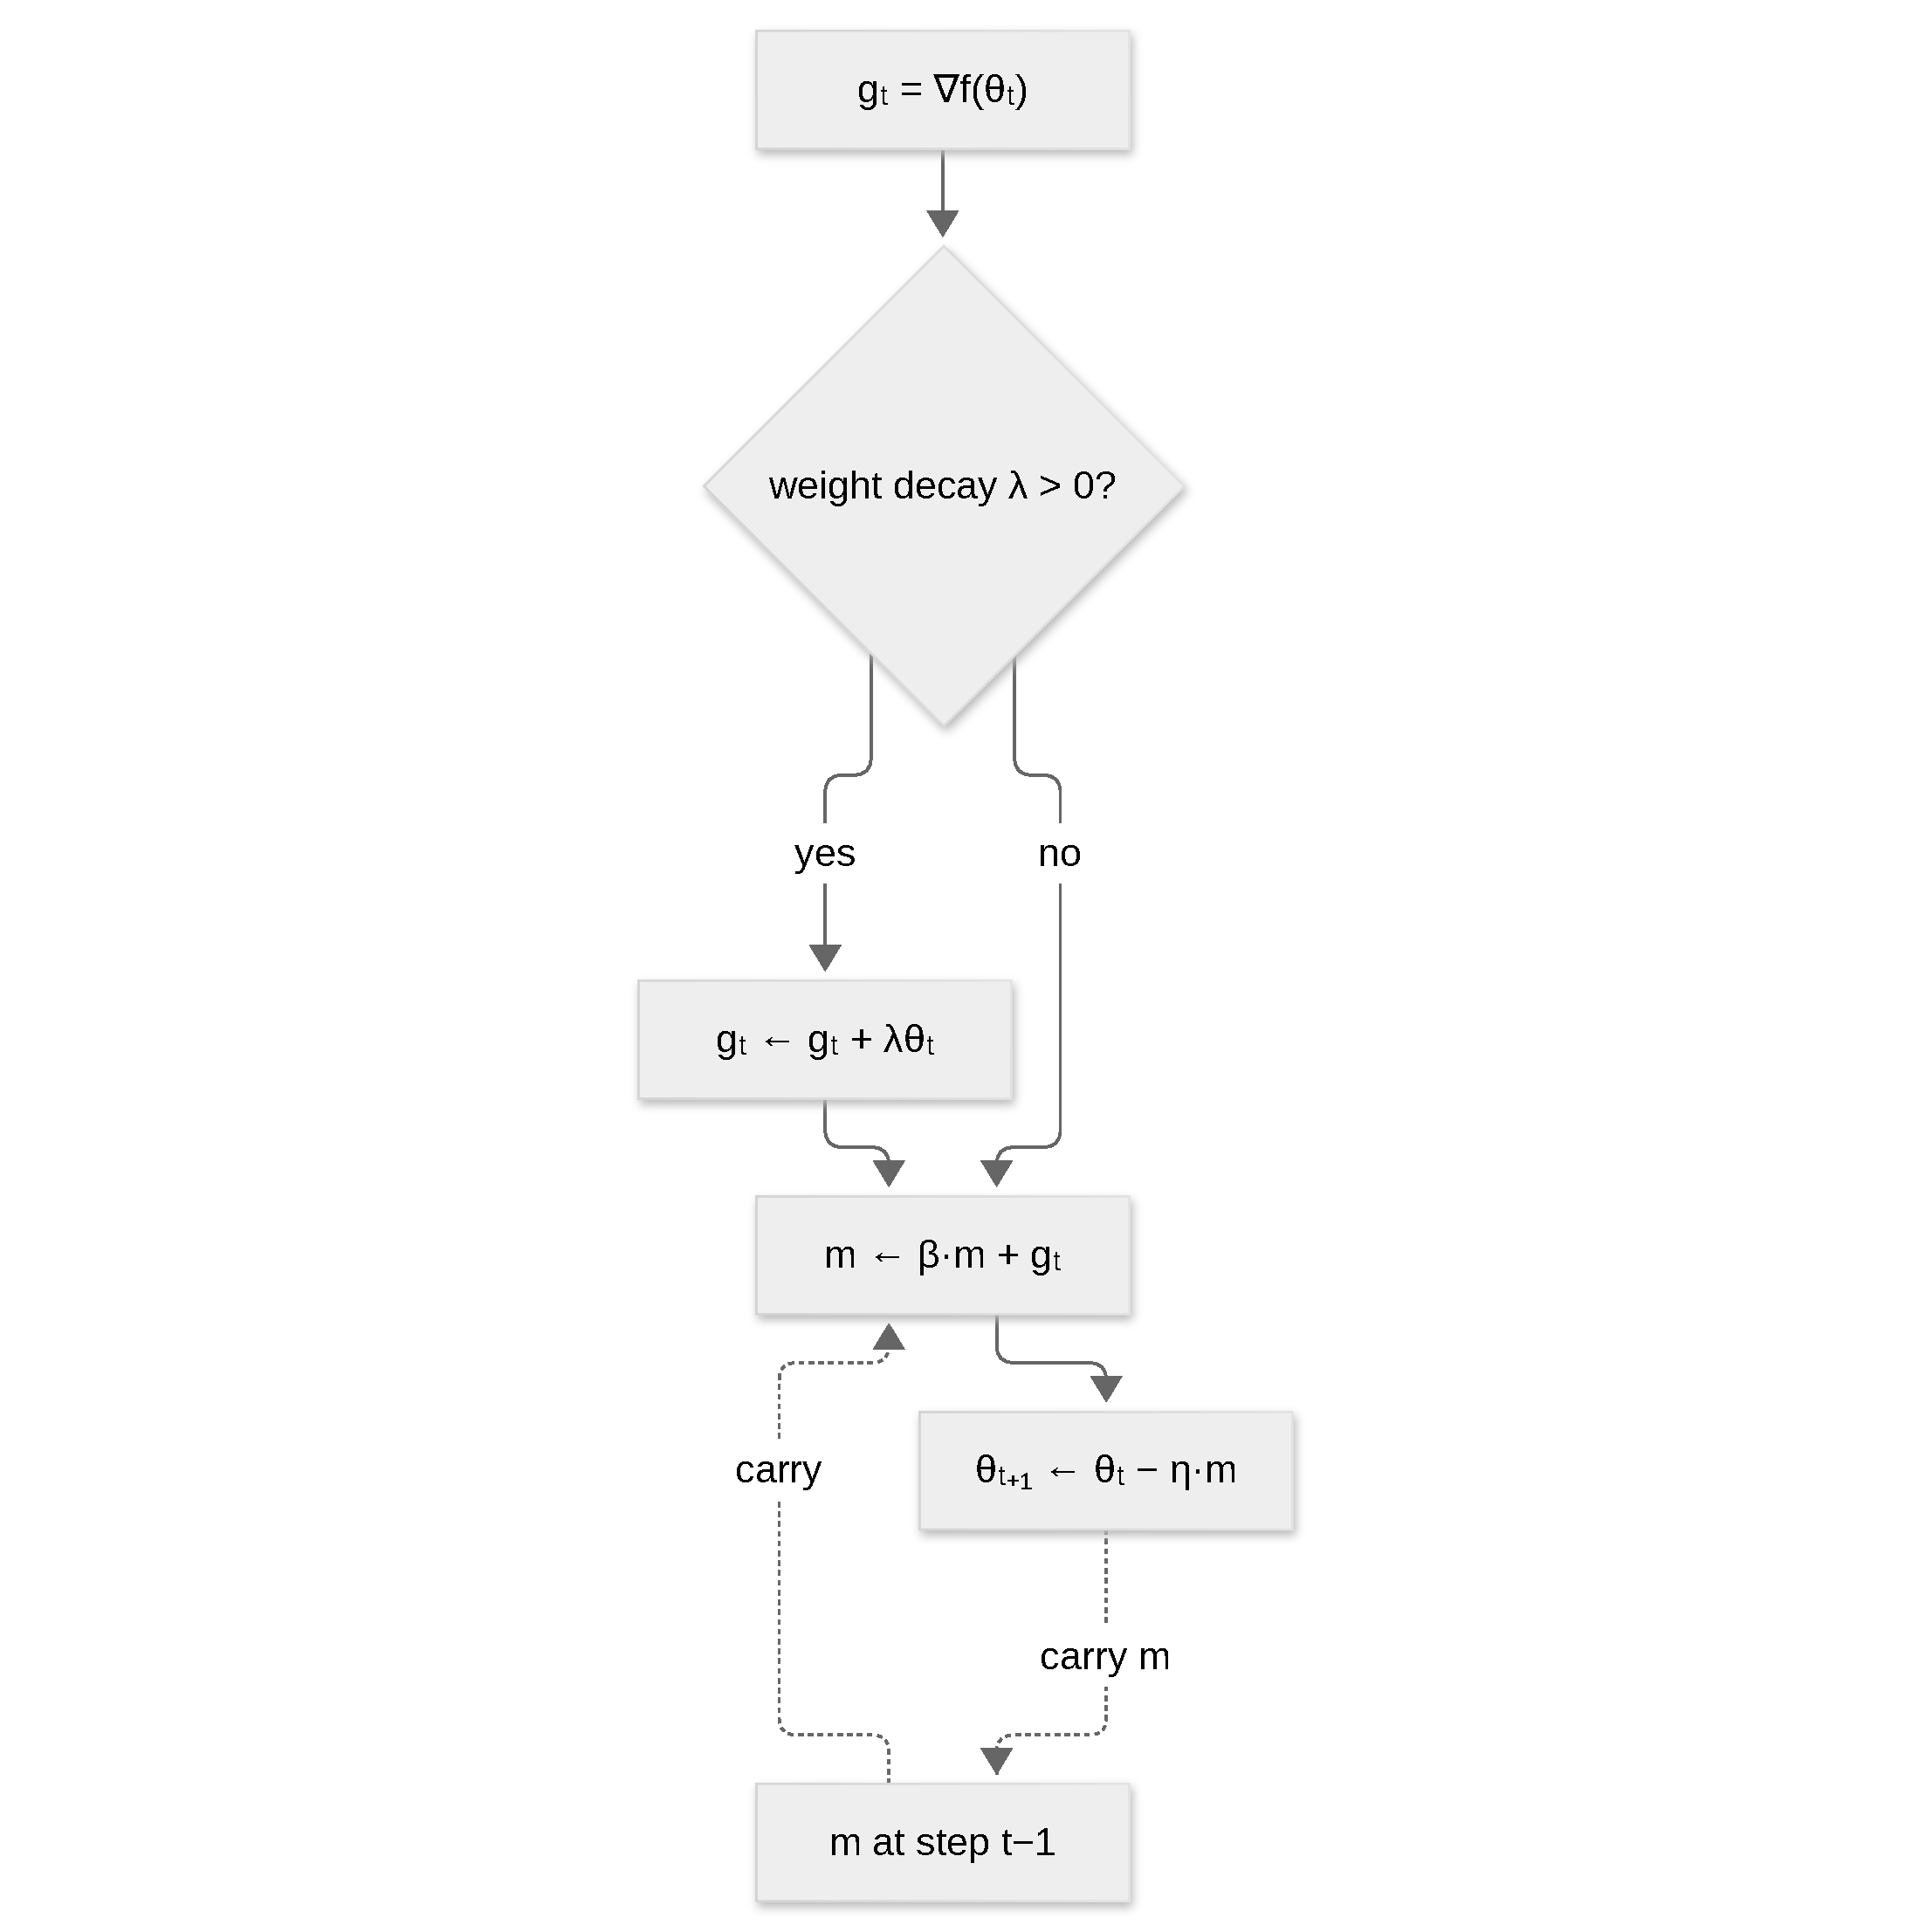
\includegraphics{../paper/figures/optimizers/sgd-momentum.pdf}}
\caption{Flujo por paso de SGD con momentum: decaimiento L2 opcional, acumulación exponencial de momentum y actualización de parámetros con paso fijo.}
\label{fig:opt-sgd-momentum}
\end{figure}
La actualización clásica acumula un búfer de momentum y luego aplica una tasa de aprendizaje fija. En cada iteración $t$, el algoritmo mantiene un promedio móvil exponencial $m_t$ de los gradientes pasados:
\begin{align}
m_t &= \beta m_{t-1} + g_t \\
\theta_{t+1} &= \theta_t - \eta m_t
\end{align}
donde $g_t = \nabla f(\theta_t)$, $\beta \in [0.8, 0.99]$ controla la decadencia del momentum y $\eta$ es la tasa de aprendizaje fija. El término de momentum actúa como velocidad: acelera el movimiento en direcciones consistentes mientras amortigua oscilaciones en direcciones variables.

\begin{algorithm}[H]
\caption{SGD con Momentum}
\label{alg:sgd-momentum}
\begin{algorithmic}[1]
\Require Parámetros iniciales $\theta_0$, tasa de aprendizaje $\eta$, coeficiente de momentum $\beta$, decadencia de peso $\lambda$
\Ensure Parámetros actualizados $\theta_T$
\State Inicializar: búfer de momentum $m \gets 0$
\For{$t = 0, 1, 2, \ldots, T-1$}
    \State Calcular gradiente: $g_t \gets \nabla f(\theta_t)$
    \If{decadencia\_de\_peso $> 0$}
        \State $g_t \gets g_t + \lambda \theta_t$ \Comment{Regularización L2}
    \EndIf
    \State Actualizar momentum: $m \gets \beta \cdot m + g_t$
    \State Actualizar parámetros: $\theta_{t+1} \gets \theta_t - \eta \cdot m$
\EndFor
\Return $\theta_T$
\end{algorithmic}
\end{algorithm}

\paragraph{Contras.}
\begin{itemize}[leftmargin=*]
\item Escasa robustez frente a la heterogeneidad de curvatura: una única tasa global no puede adaptarse a todos los grupos de parámetros.
\item Fuerte dependencia de programaciones de tasa de aprendizaje cuidadosamente diseñadas.
\end{itemize}

\paragraph{Ventajas.}
\begin{itemize}[leftmargin=*]
\item Baja sobrecarga de memoria: un único búfer de momentum por parámetro.
\item Fuerte generalización cuando se ajusta cuidadosamente, y una actualización simple de implementar.
\end{itemize}

\paragraph{Adam y AdamW.}
\begin{figure}[H]
\centering
\fitfigure{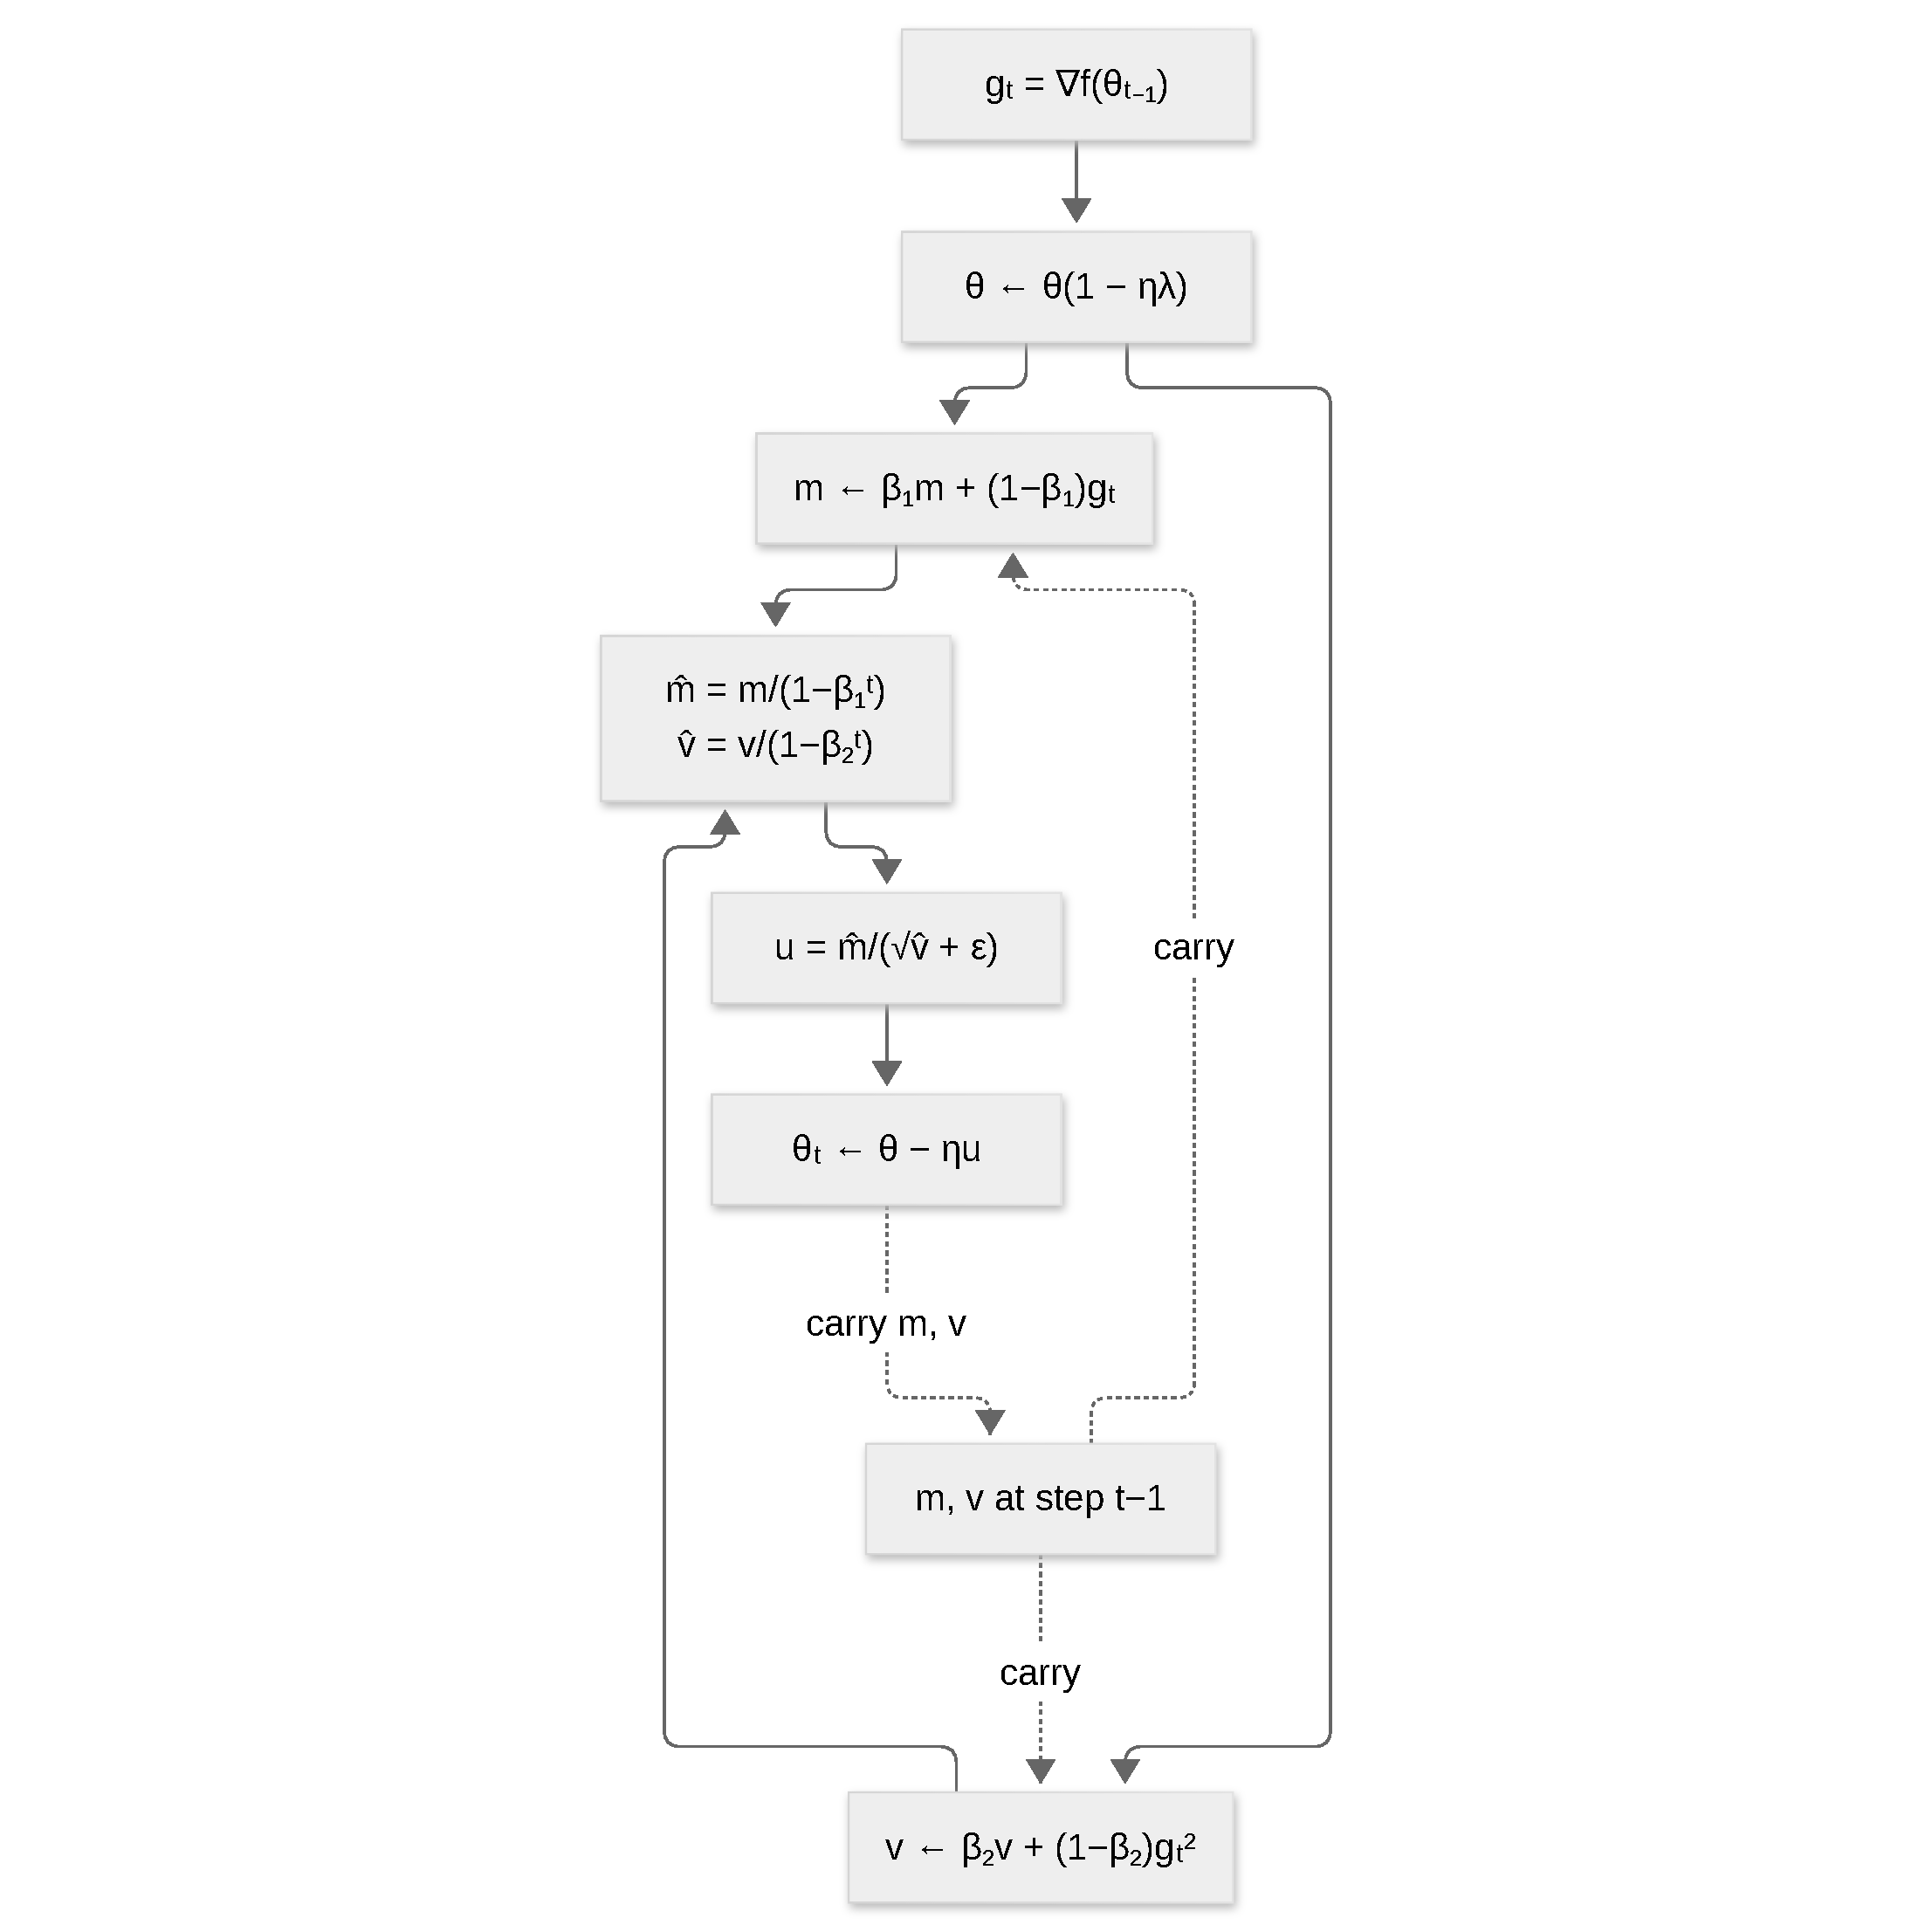
\includegraphics{../paper/figures/optimizers/adamw.pdf}}
\caption{Flujo por paso de AdamW: decaimiento de pesos desacoplado, EMAs de primer y segundo momento, corrección de sesgo y actualización adaptativa elemento a elemento.}
\label{fig:opt-adamw}
\end{figure}
Adam rastrea promedios móviles exponenciales tanto del primer momento (media) como del segundo momento (varianza no centrada) para lograr tasas de aprendizaje adaptativas elemento a elemento. La regla de actualización es:
\begin{align}
m_t &= \beta_1 m_{t-1} + (1-\beta_1) g_t \\
v_t &= \beta_2 v_{t-1} + (1-\beta_2) g_t^2 \\
\hat{m}_t &= \frac{m_t}{1-\beta_1^t}, \quad \hat{v}_t = \frac{v_t}{1-\beta_2^t} \quad \text{(corrección de sesgo)} \\
\theta_{t+1} &= \theta_t - \eta \left(\frac{\hat{m}_t}{\sqrt{\hat{v}_t}+\epsilon}\right)
\end{align}
AdamW introduce una modificación crucial: la decadencia de peso se aplica directamente a los parámetros (desacoplada de los gradientes): $\theta_t \gets \theta_t(1-\eta\lambda)$ en lugar de añadir $\lambda\theta_t$ al gradiente. Este desacoplamiento evita que el escalado adaptativo interfiera con la fuerza de la regularización.

\begin{algorithm}[H]
\caption{AdamW (Adam con Decadencia de Peso Desacoplada)}
\label{alg:adamw}
\begin{algorithmic}[1]
\Require Parámetros iniciales $\theta_0$, tasa de aprendizaje $\eta$, tasas de decadencia exponencial $\beta_1, \beta_2 \in [0,1)$
\Require Constante de momentum $\epsilon$, decadencia de peso $\lambda$
\Ensure Parámetros actualizados $\theta_T$
\State Inicializar: primer momento $m \gets 0$, segundo momento $v \gets 0$, contador de pasos $t \gets 0$
\For{$t = 1, 2, \ldots, T$}
    \State Calcular gradiente: $g_t \gets \nabla f(\theta_{t-1})$
    \State Decadencia de peso (desacoplada): $\theta_{t-1} \gets \theta_{t-1}(1 - \eta\lambda)$
    \State Actualizar momentos: $m \gets \beta_1 m + (1-\beta_1) g_t$
    \State $v \gets \beta_2 v + (1-\beta_2) g_t^2$
    \State Corrección de sesgo: $\hat{m} \gets m / (1 - \beta_1^t)$, $\hat{v} \gets v / (1 - \beta_2^t)$
    \State Actualizar parámetros: $\theta_t \gets \theta_{t-1} - \eta (\hat{m} / (\sqrt{\hat{v}} + \epsilon))$
\EndFor
\Return $\theta_T$
\end{algorithmic}
\end{algorithm}

\paragraph{Contras.}
\begin{itemize}[leftmargin=*]
\item Almacena tensores de primer y segundo momento para cada parámetro, duplicando la memoria del estado del optimizador respecto a SGD.
\item El escalado adaptativo elemento a elemento puede interferir con la regularización si el decaimiento de pesos no se desacopla.
\end{itemize}

\paragraph{Ventajas.}
\begin{itemize}[leftmargin=*]
\item Línea base práctica para el ajuste fino de transformadores: convergencia rápida y tolerancia a la variación de hiperparámetros.
\item El decaimiento de pesos desacoplado mantiene la fuerza de la regularización independiente del escalado adaptativo.
\end{itemize}

\paragraph{RAdam (Adam Rectificado).}
\begin{figure}[H]
\centering
\fitfigure{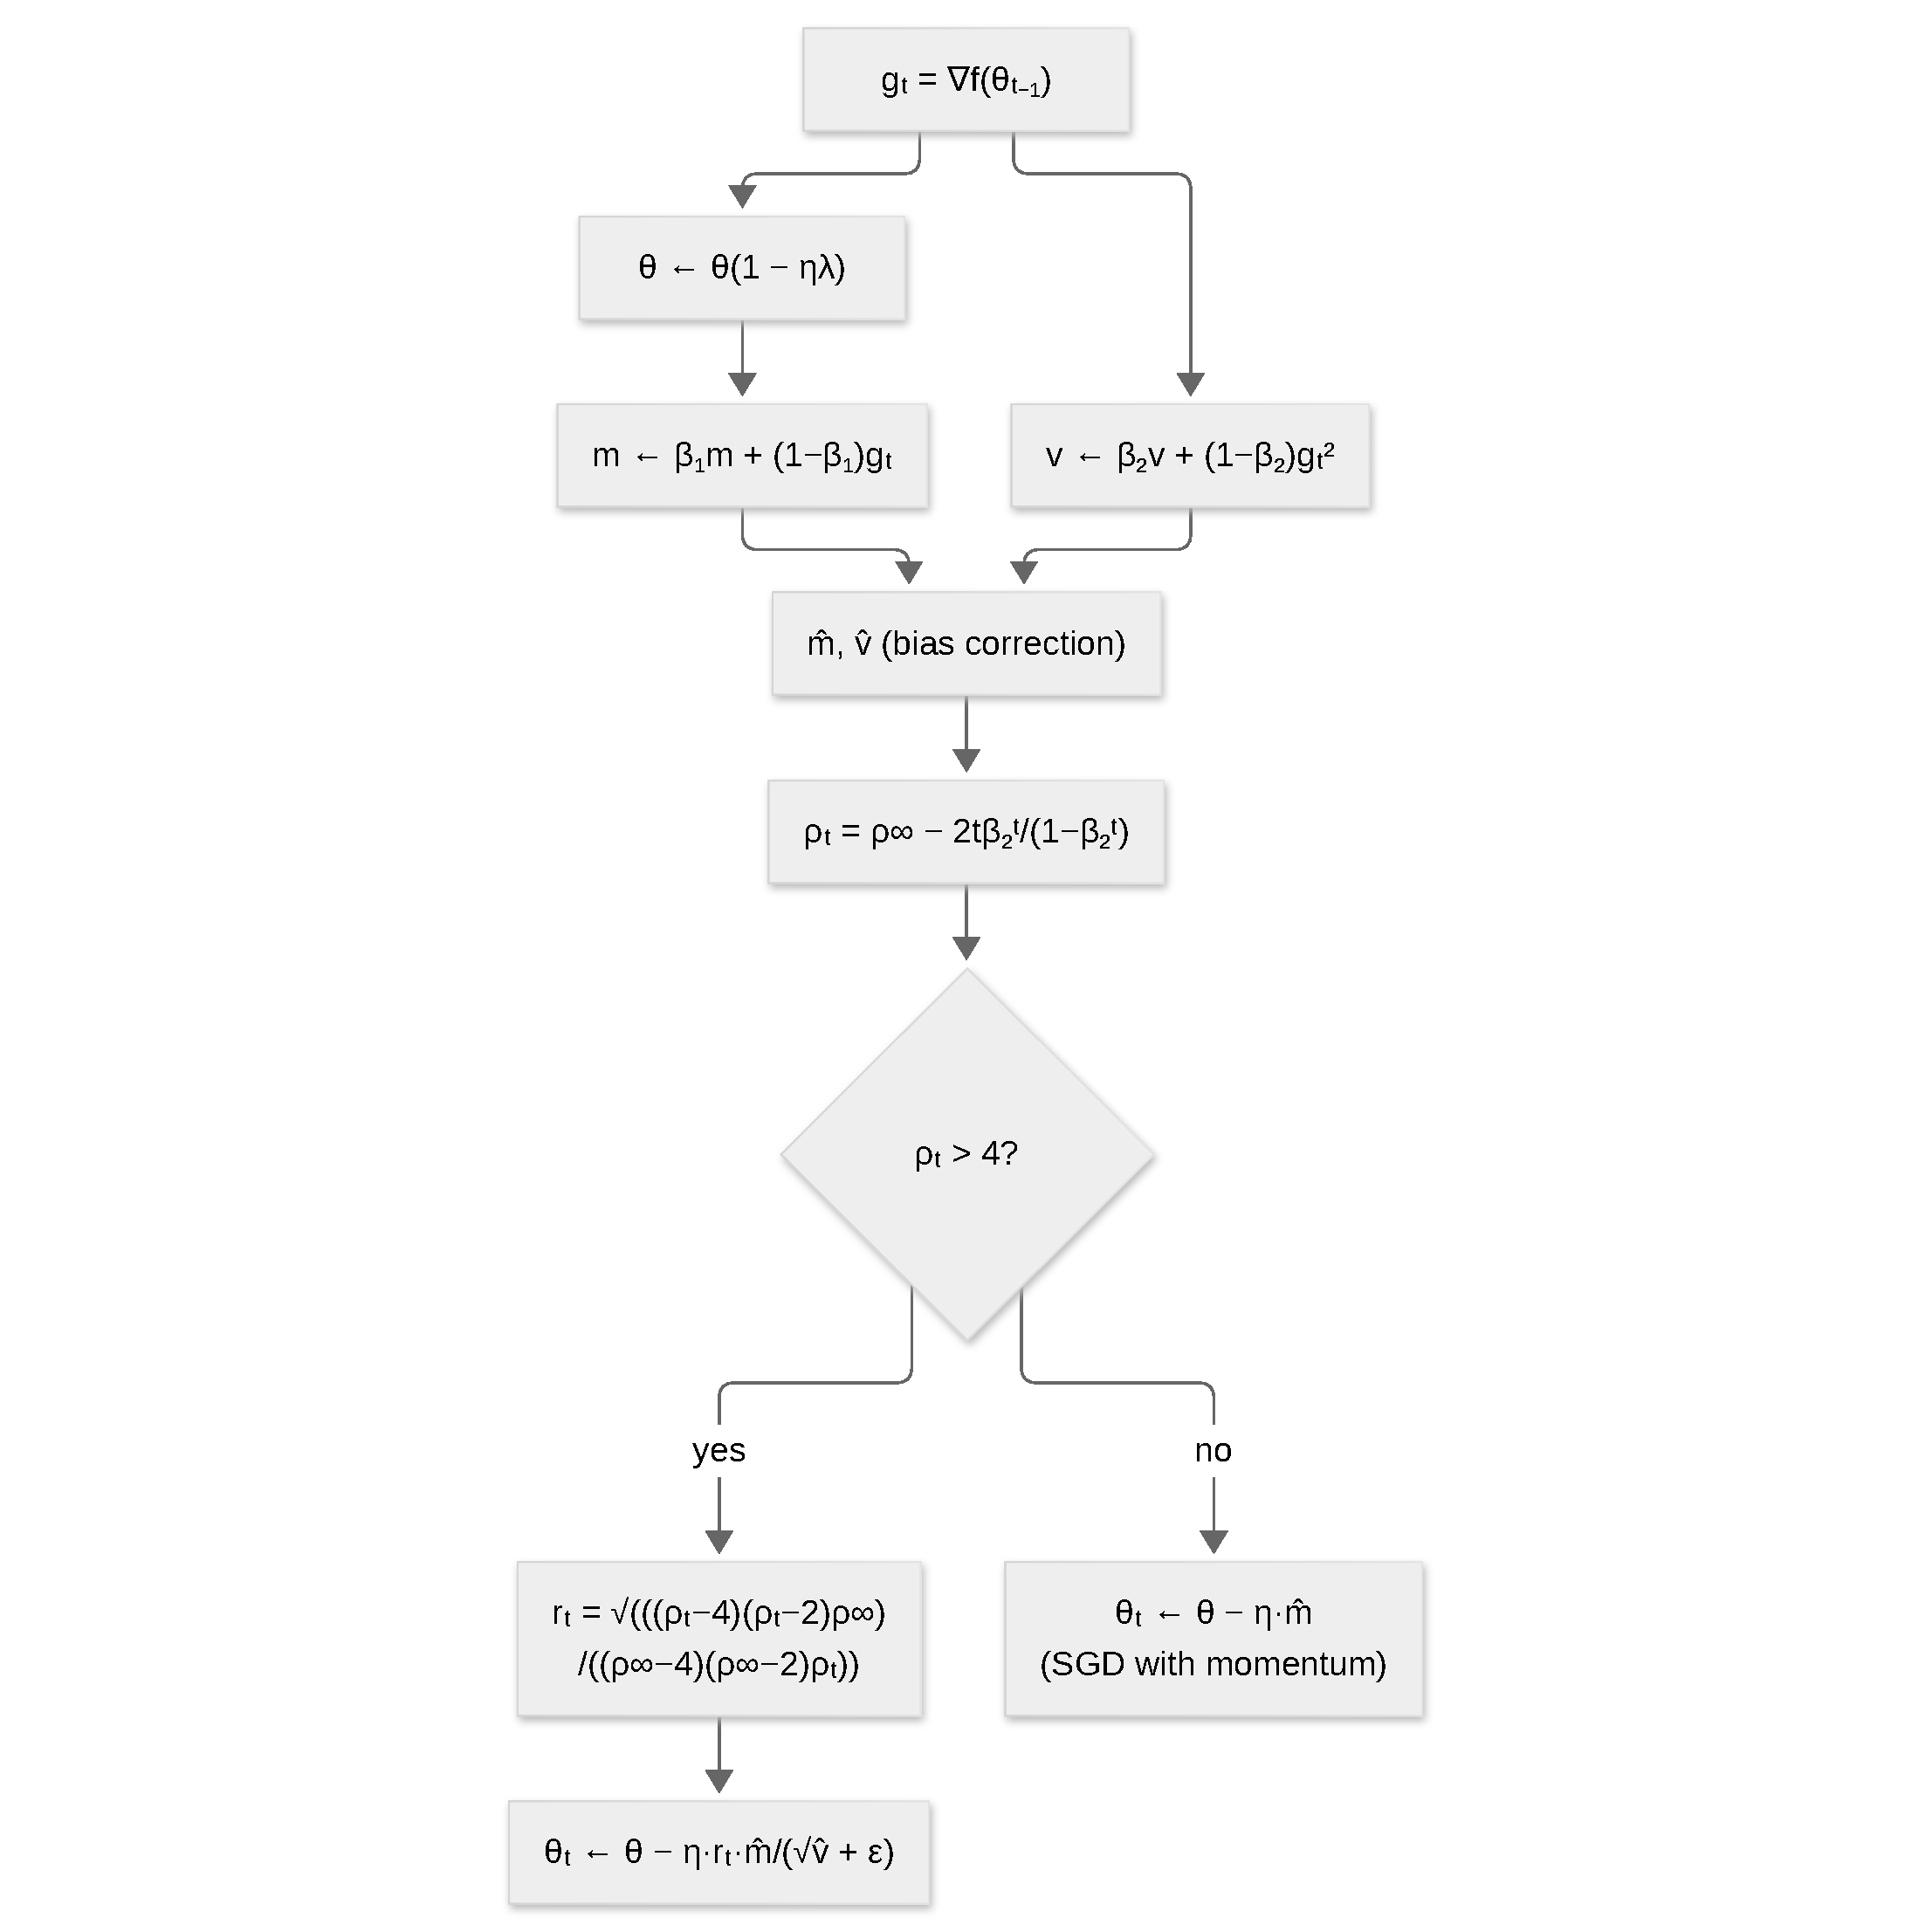
\includegraphics{../paper/figures/optimizers/radam.pdf}}
\caption{Flujo por paso de RAdam: rectificación por ventana SMA con retroceso a SGD con momentum en los primeros pasos.}
\label{fig:opt-radam}
\end{figure}
RAdam aborda la inestabilidad de Adam en el entrenamiento temprano rectificando dinámicamente la tasa de aprendizaje adaptativa. La observación clave es que el segundo momento $v_t$ tiene una varianza muy alta en los primeros pasos, causando un escalado adaptativo poco fiable. RAdam calcula la longitud efectiva de la ventana de promedio móvil simple (SMA):
\[\rho_t = \rho_{\infty} - \frac{2t\beta_2^t}{1-\beta_2^t}, \quad \text{donde} \quad \rho_{\infty} = \frac{2}{1-\beta_2}-1\]
Cuando $\rho_t > 4$ (suficientes muestras para la estimación de varianza), RAdam aplica el escalado adaptativo con un término de rectificación:
\[r_t = \sqrt{\frac{(\rho_t-4)(\rho_t-2)\rho_{\infty}}{(\rho_{\infty}-4)(\rho_{\infty}-2)\rho_t}}, \quad \theta_{t+1} = \theta_t - \eta r_t \frac{\hat{m}_t}{\sqrt{\hat{v}_t}+\epsilon}\]
Cuando $\rho_t \leq 4$, RAdam retrocede a SGD con momentum: $\theta_{t+1} = \theta_t - \eta\hat{m}_t$.

\begin{algorithm}[H]
\caption{RAdam (Adam Rectificado)}
\label{alg:radam}
\begin{algorithmic}[1]
\Require Parámetros iniciales $\theta_0$, tasa de aprendizaje $\eta$, $\beta_1, \beta_2$, decadencia de peso $\lambda$
\Ensure Parámetros actualizados $\theta_T$
\State Inicializar: $m \gets 0$, $v \gets 0$, $t \gets 0$
\State Calcular: $\rho_\infty \gets 2/(1-\beta_2) - 1$
\For{$t = 1, 2, \ldots, T$}
    \State $g_t \gets \nabla f(\theta_{t-1})$
    \If{decadencia\_de\_peso $> 0$}
        \State $\theta_{t-1} \gets \theta_{t-1}(1 - \eta\lambda)$
    \EndIf
    \State $m \gets \beta_1 m + (1-\beta_1) g_t$
    \State $v \gets \beta_2 v + (1-\beta_2) g_t^2$
    \State $\hat{m} \gets m/(1-\beta_1^t)$, $\hat{v} \gets v/(1-\beta_2^t)$
    \State $\rho_t \gets \rho_\infty - 2t \beta_2^t / (1 - \beta_2^t)$
    \If{$\rho_t > 4$}
        \State $r_t \gets \sqrt{((\rho_t-4)(\rho_t-2)\rho_\infty) / ((\rho_\infty-4)(\rho_\infty-2)\rho_t)}$
        \State $\theta_t \gets \theta_{t-1} - \eta r_t \hat{m} / (\sqrt{\hat{v}} + \epsilon)$
    \Else
        \State $\theta_t \gets \theta_{t-1} - \eta \hat{m}$ \Comment{SGD con momentum}
    \EndIf
\EndFor
\Return $\theta_T$
\end{algorithmic}
\end{algorithm}

\paragraph{Contras.}
\begin{itemize}[leftmargin=*]
\item Añade contabilidad de rectificación sobre el estado de momentos de Adam.
\item El beneficio se reduce cuando ya se usa una programación de calentamiento bien ajustada.
\end{itemize}

\paragraph{Ventajas.}
\begin{itemize}[leftmargin=*]
\item Elimina la necesidad de calentamiento manual al rectificar la tasa adaptativa.
\item Retrocede con elegancia a SGD con momentum mientras las estimaciones de varianza no son fiables, mejorando la robustez.
\end{itemize}

\subsection{Momentum Avanzado y Reducción de Varianza (2024--2025)}
\paragraph{Adan (Momentum Nesterov Adaptativo).}
\begin{figure}[H]
\centering
\fitfigure{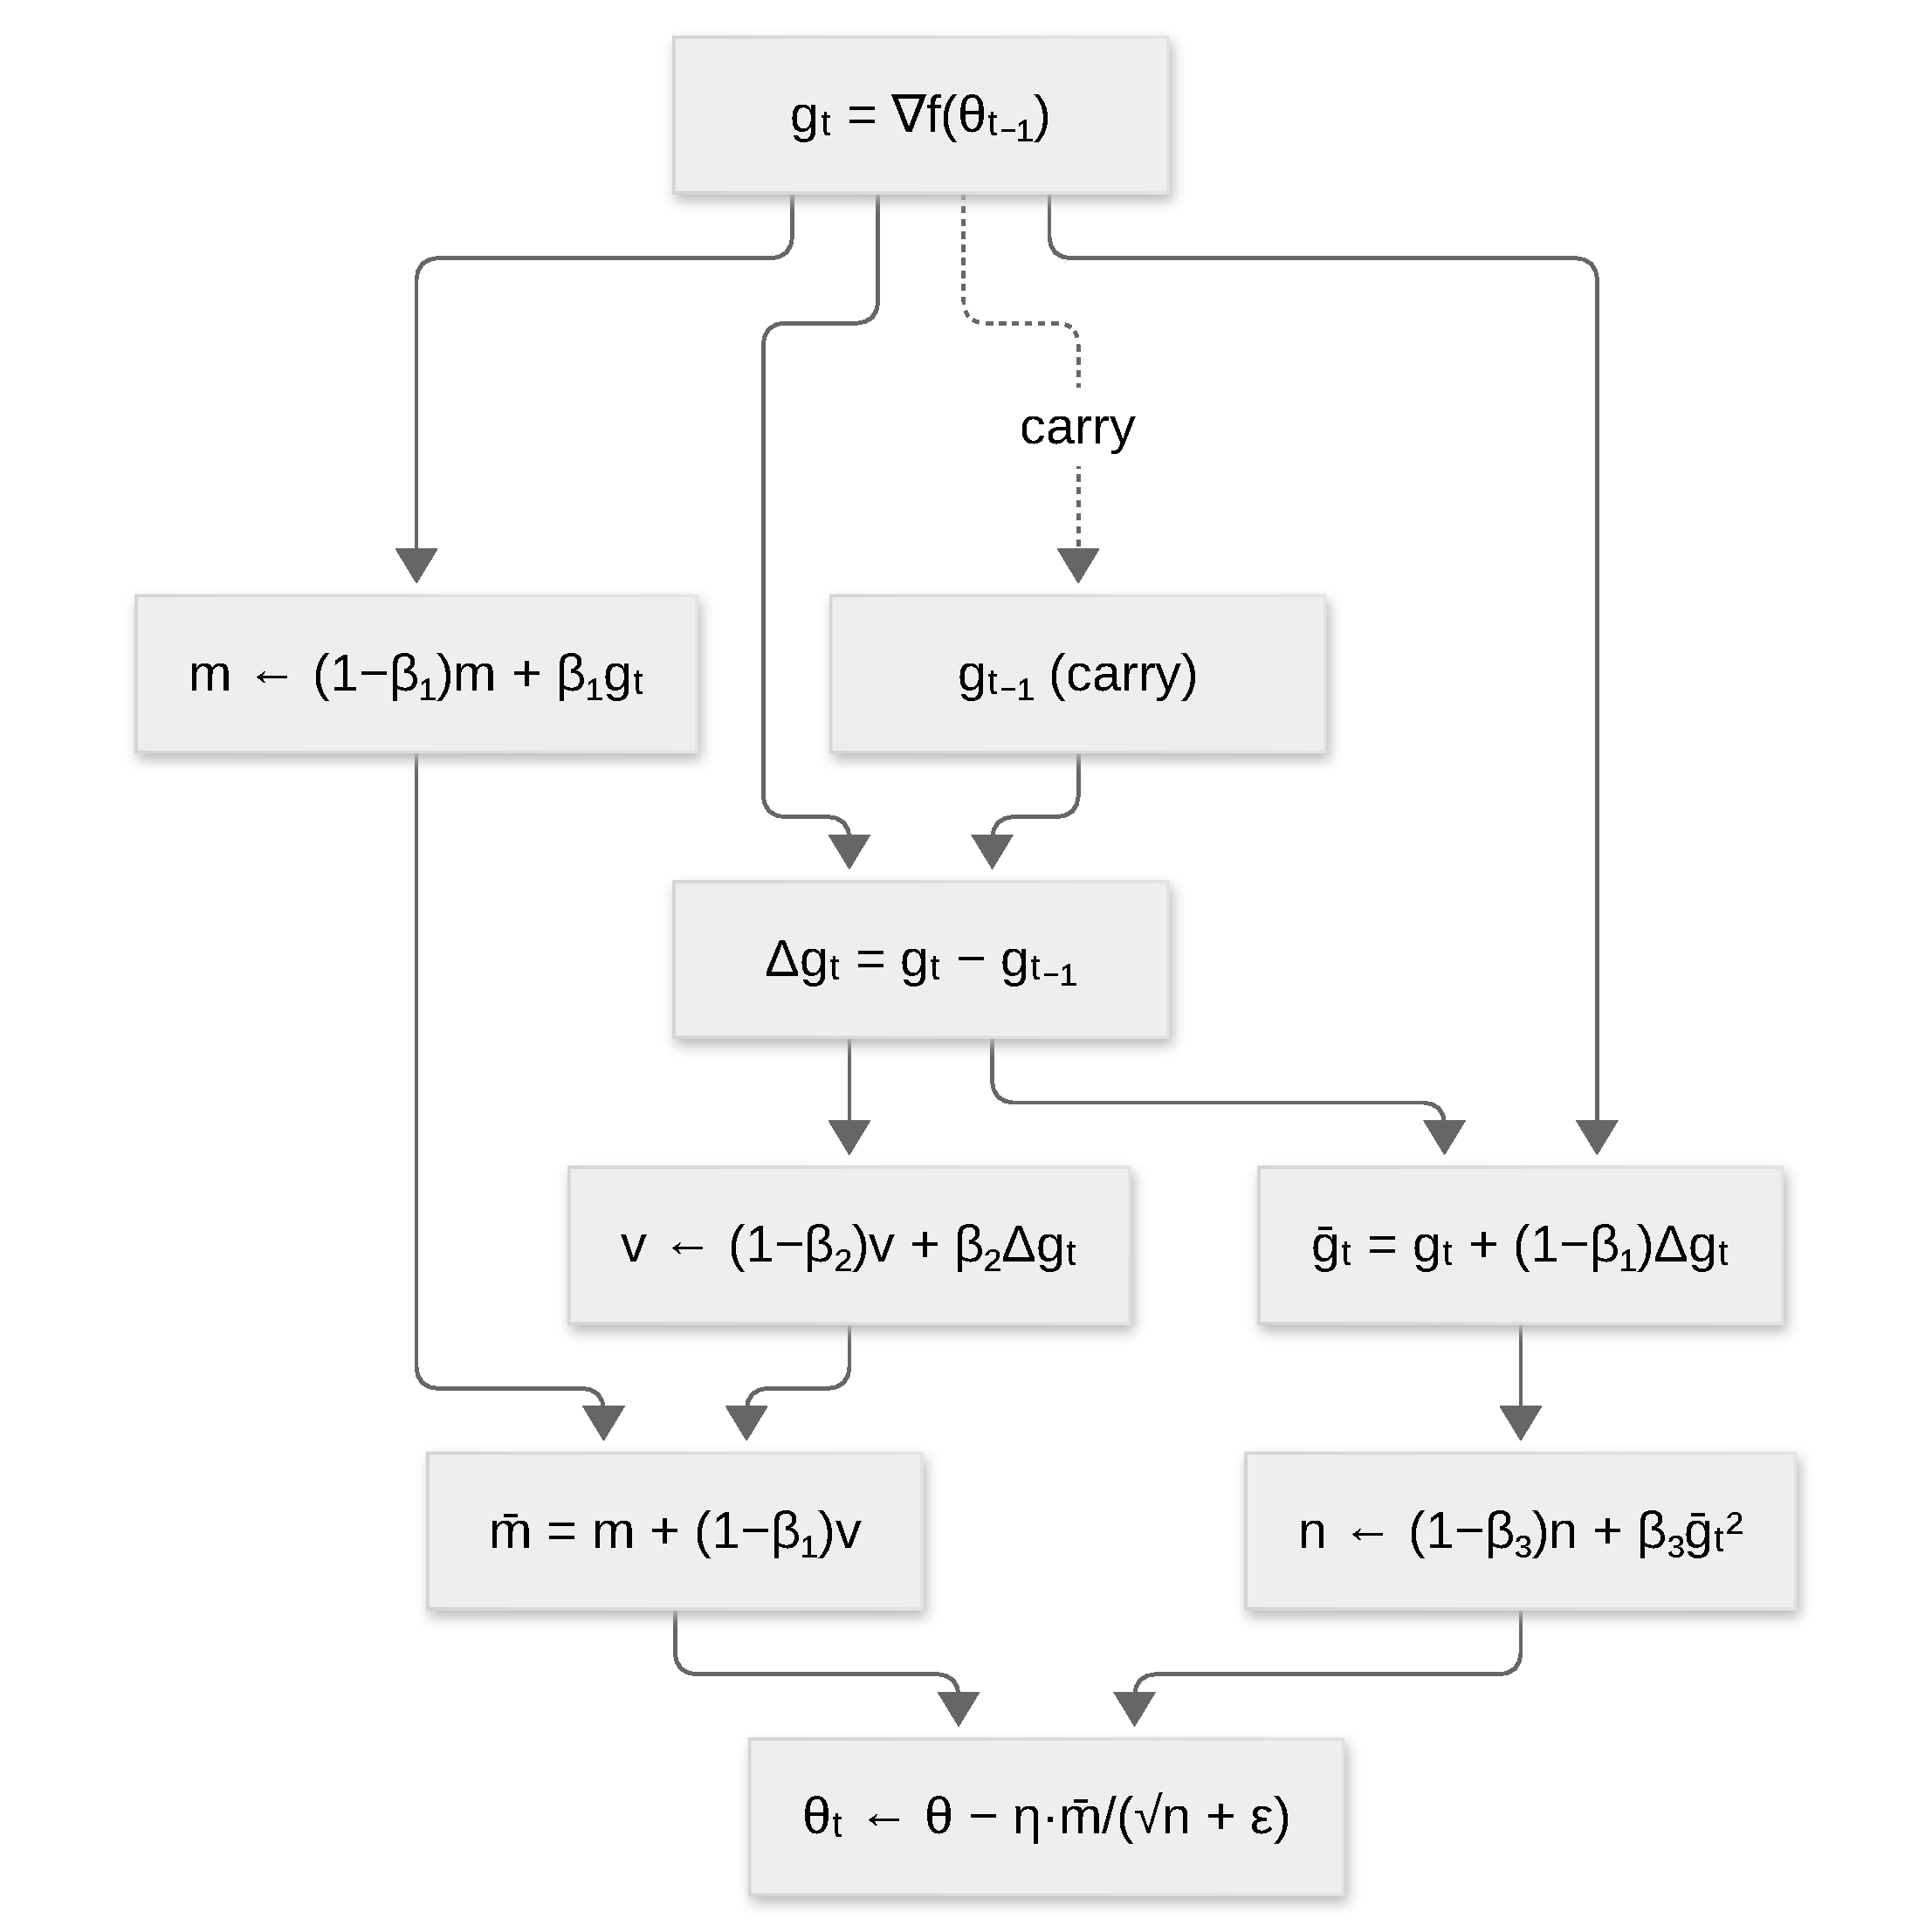
\includegraphics{../paper/figures/optimizers/adan.pdf}}
\caption{Flujo por paso de Adan: estimación de momentum de Nesterov a partir de la diferencia de gradientes, con tres búferes de estado y un paso de momentum combinado.}
\label{fig:opt-adan}
\end{figure}
Adan reformula la aceleración de Nesterov sin el cálculo de gradiente adicional requerido por el SGD Nesterov clásico. El algoritmo mantiene tres búferes de momentum:
\begin{align}
m_t &= (1-\beta_1)m_{t-1} + \beta_1 g_t \quad\text{(primer momento)} \\
v_t &= (1-\beta_2)v_{t-1} + \beta_2(g_t - g_{t-1}) \quad\text{(velocidad/diferencia de gradientes)} \\
n_t &= (1-\beta_3)n_{t-1} + \beta_3[g_t + (1-\beta_1)(g_t-g_{t-1})]^2 \quad\text{(segundo momento Nesterov)}
\end{align}
El término de \textbf{Estimación de Momentum Nesterov} (NME) $\bar{g}_t = g_t + (1-\beta_1)(g_t-g_{t-1})$ estima el gradiente en una posición futura sin evaluarlo. La actualización combina el momentum con la velocidad:
\[\bar{m}_t = m_t + (1-\beta_1)v_t, \quad \theta_{t+1} = \theta_t - \eta\frac{\bar{m}_t}{\sqrt{n_t}+\epsilon}\]

\begin{algorithm}[H]
\caption{Adan (Momentum Nesterov Adaptativo)}
\label{alg:adan}
\begin{algorithmic}[1]
\Require Parámetros iniciales $\theta_0$, tasa de aprendizaje $\eta$, $\beta_1, \beta_2, \beta_3 \in (0,1)$
\Ensure Parámetros actualizados $\theta_T$
\State Inicializar: $m \gets 0$, $v \gets 0$, $n \gets 0$, $g_{-1} \gets 0$ (gradiente anterior)
\For{$t = 1, 2, \ldots, T$}
    \State $g_t \gets \nabla f(\theta_{t-1})$
    \State $m \gets (1-\beta_1) m + \beta_1 g_t$
    \State $\Delta g_t \gets g_t - g_{t-1}$
    \State $v \gets (1-\beta_2) v + \beta_2 \Delta g_t$
    \State Estimación Nesterov: $\bar{g}_t \gets g_t + (1-\beta_1) \Delta g_t$
    \State $n \gets (1-\beta_3) n + \beta_3 \bar{g}_t^2$
    \State Momentum combinado: $\bar{m} \gets m + (1-\beta_1) v$
    \State $\theta_t \gets \theta_{t-1} - \eta (\bar{m} / (\sqrt{n} + \epsilon))$
    \State $g_{t-1} \gets g_t$
\EndFor
\Return $\theta_T$
\end{algorithmic}
\end{algorithm}

\paragraph{Contras.}
\begin{itemize}[leftmargin=*]
\item Tres búferes tipo momentum aumentan la sobrecarga de memoria respecto a Adam.
\item Contabilidad adicional de la diferencia de gradientes en cada paso.
\end{itemize}

\paragraph{Ventajas.}
\begin{itemize}[leftmargin=*]
\item Aceleración estilo Nesterov sin una evaluación adicional del gradiente.
\item Convergencia rápida en arquitecturas diversas (CNN, GAN, transformadores).
\end{itemize}

\paragraph{ADOPT (Adam con Ajuste Óptimo Podado).}
\begin{figure}[H]
\centering
\fitfigure{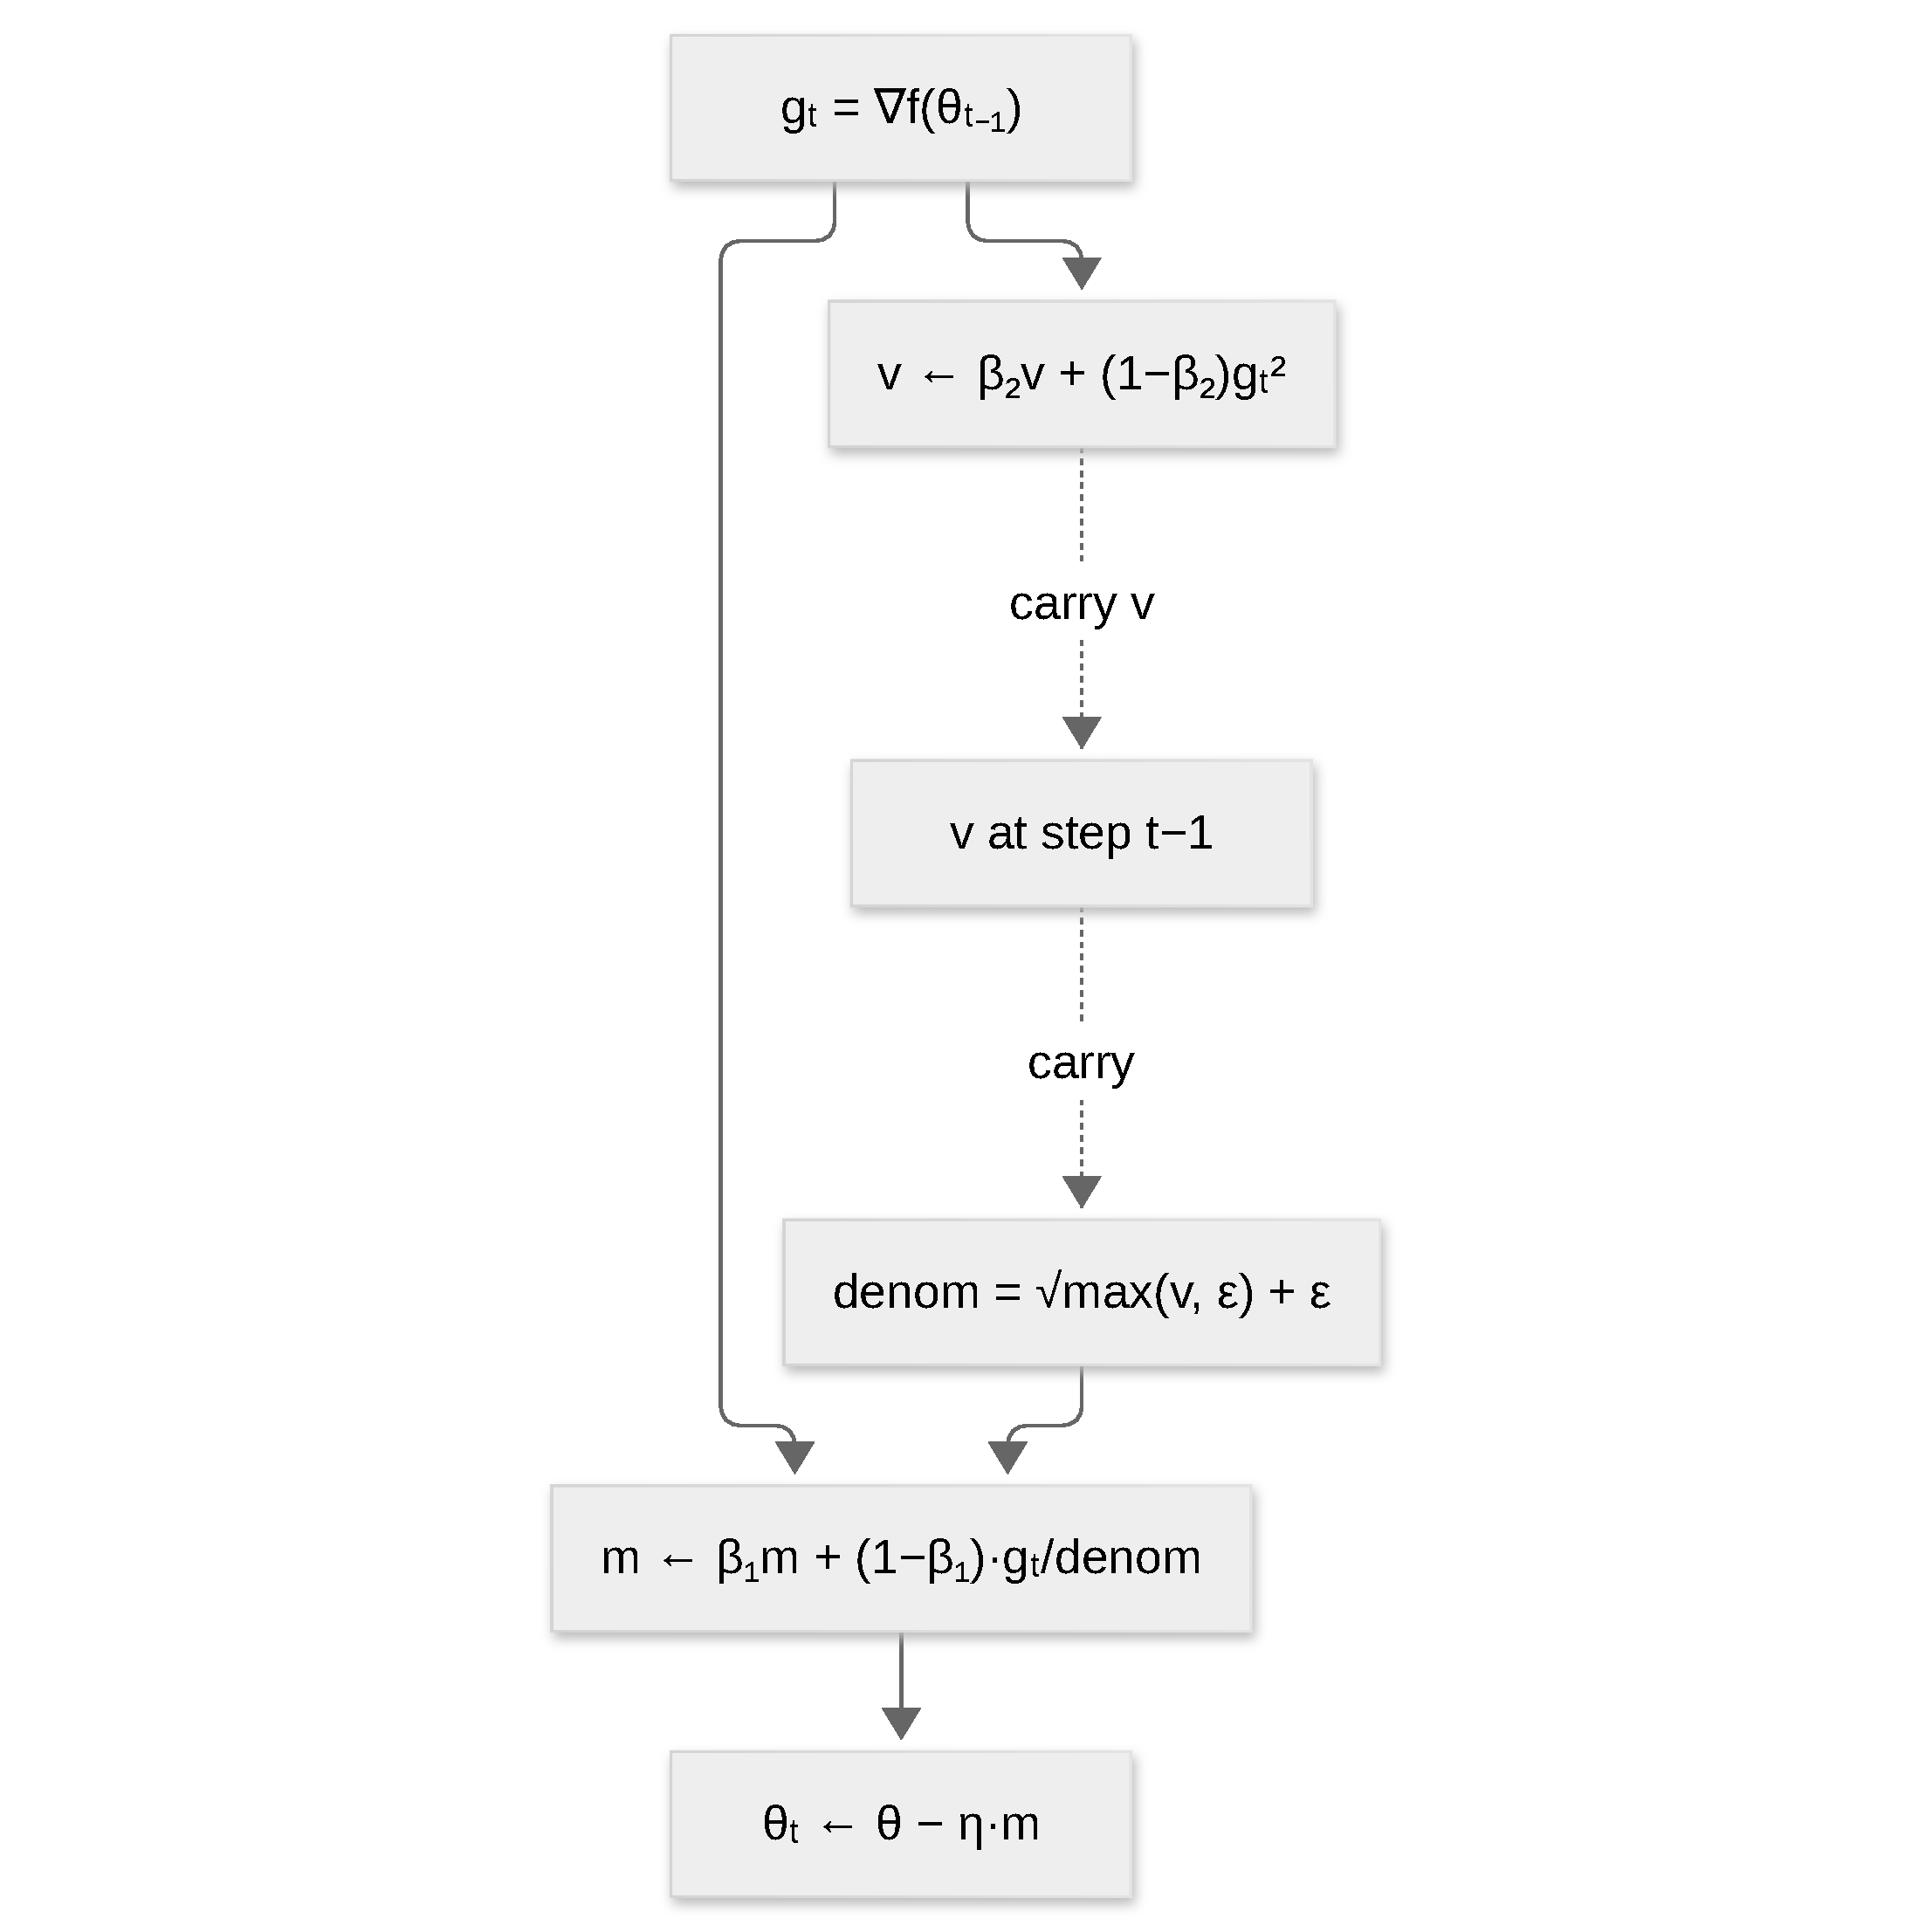
\includegraphics{../paper/figures/optimizers/adopt.pdf}}
\caption{Flujo por paso de ADOPT: el segundo momento del paso anterior normaliza el gradiente actual antes de actualizar el primer momento.}
\label{fig:opt-adopt}
\end{figure}
ADOPT corrige un problema teórico fundamental en Adam: el gradiente aparece tanto en la estimación del primer momento como en la del segundo momento, creando circularidad. ADOPT \textbf{desacopla} utilizando el segundo momento del paso anterior para el denominador:
\begin{align}
v_t &= \beta_2 v_{t-1} + (1-\beta_2)g_t^2 \\
m_t &= \beta_1 m_{t-1} + (1-\beta_1)\frac{g_t}{\sqrt{v_{t-1}}+\epsilon} \quad\text{(usa $v_{t-1}$, no $v_t$)} \\
\theta_{t+1} &= \theta_t - \eta m_t
\end{align}

\begin{algorithm}[H]
\caption{ADOPT (Adam con Ajuste Óptimo Podado)}
\label{alg:adopt}
\begin{algorithmic}[1]
\Require Parámetros iniciales $\theta_0$, tasa de aprendizaje $\eta$, $\beta_1, \beta_2$, tolerancia $\epsilon$
\Ensure Parámetros actualizados $\theta_T$
\State Inicializar: $m \gets 0$, $v \gets 0$
\For{$t = 1, 2, \ldots, T$}
    \State $g_t \gets \nabla f(\theta_{t-1})$
    \If{decadencia\_de\_peso $> 0$}
        \State $\theta_{t-1} \gets \theta_{t-1}(1 - \eta\lambda)$
    \EndIf
    \State Usar segundo momento \textbf{anterior}: $\text{denom} \gets \sqrt{\max(v, \epsilon)} + \epsilon$
    \State Actualizar primer momento usando varianza anterior: $m \gets \beta_1 m + (1-\beta_1)(g_t / \text{denom})$
    \State Actualizar segundo momento con gradiente \textbf{actual}: $v \gets \beta_2 v + (1-\beta_2) g_t^2$
    \State $\theta_t \gets \theta_{t-1} - \eta m$
\EndFor
\Return $\theta_T$
\end{algorithmic}
\end{algorithm}

\paragraph{Contras.}
\begin{itemize}[leftmargin=*]
\item Requiere conservar el segundo momento anterior como denominador explícito.
\item Las ganancias empíricas dependen de la arquitectura y del ajuste.
\end{itemize}

\paragraph{Ventajas.}
\begin{itemize}[leftmargin=*]
\item Elimina la circularidad del gradiente de Adam y alcanza la tasa óptima $O(1/\sqrt{T})$ con \textbf{cualquier} $\beta_2 \in (0,1)$, sin suposiciones de ruido acotado.
\item Reemplazo directo de Adam con rendimiento empírico comparable o superior en visión, PLN, RL y modelado generativo.
\end{itemize}

\paragraph{AdEMAMix (Mezcla de Promedios Móviles Exponenciales).}
\begin{figure}[H]
\centering
\fitfigure{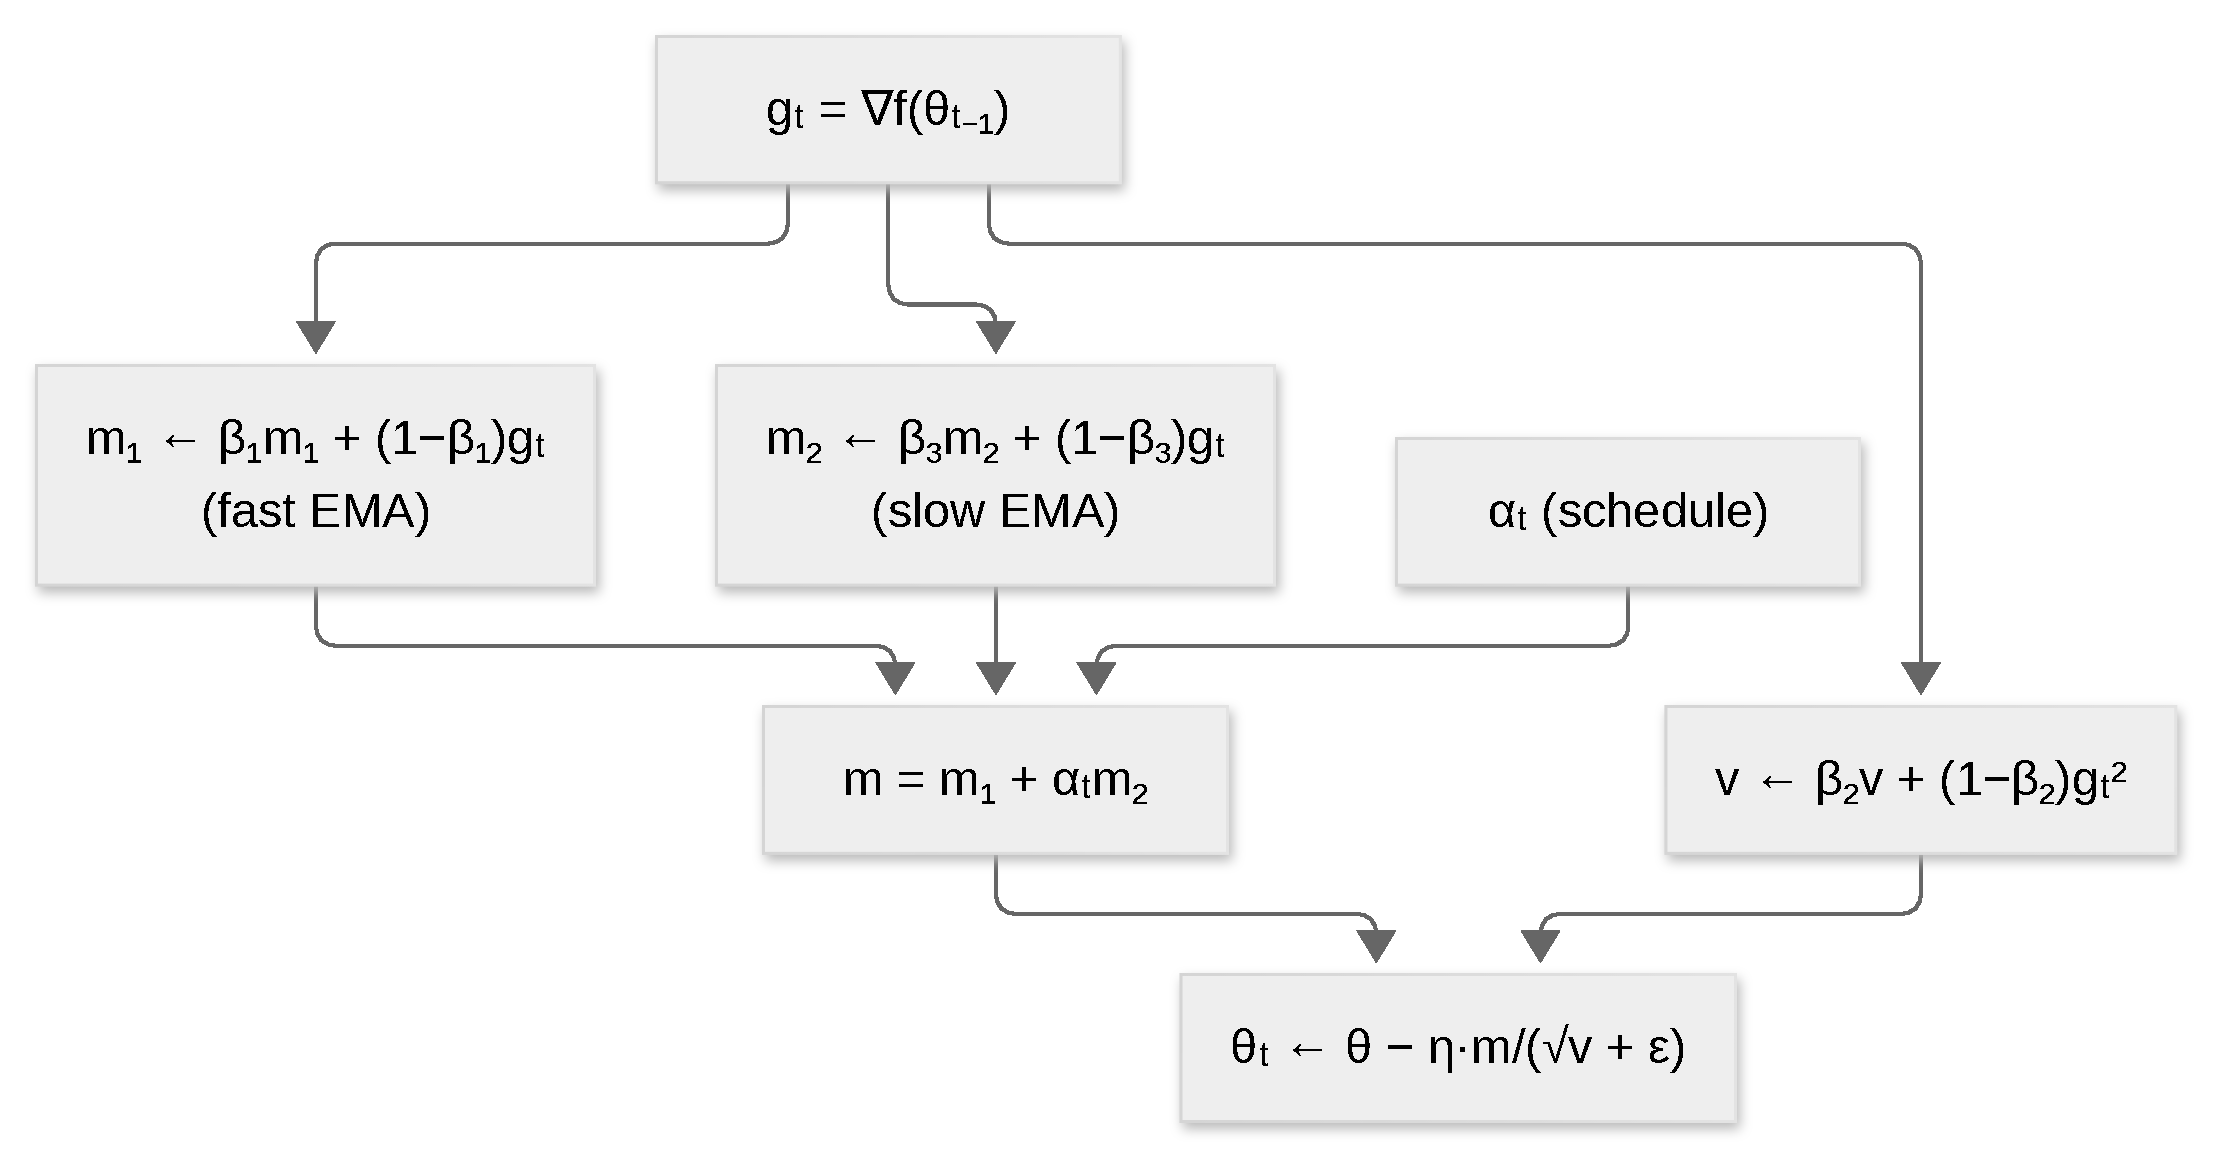
\includegraphics{../paper/figures/optimizers/ademamix.pdf}}
\caption{Flujo por paso de AdEMAMix: EMAs rápida y lenta en paralelo, mezcladas con un peso programado $\alpha_t$ antes de la actualización adaptativa.}
\label{fig:opt-ademamix}
\end{figure}
AdEMAMix reemplaza el EMA único de gradientes de Adam por una \textbf{mezcla de dos EMA}: uno de decadencia rápida y otro de decadencia lenta. Esto aborda la observación de que los gradientes siguen siendo informativos durante decenas de miles de pasos, no solo cientos:
\begin{align}
m_{1,t} &= \beta_1 m_{1,t-1} + (1-\beta_1)g_t \quad\text{(EMA rápido, $\beta_1 \approx 0.9$)} \\
m_{2,t} &= \beta_3 m_{2,t-1} + (1-\beta_3)g_t \quad\text{(EMA lento, $\beta_3 \approx 0.9999$)} \\
v_t &= \beta_2 v_{t-1} + (1-\beta_2)g_t^2 \\
m_t &= m_{1,t} + \alpha_t m_{2,t} \quad\text{(mezcla con peso programado $\alpha_t$)} \\
\theta_{t+1} &= \theta_t - \eta\frac{m_t}{\sqrt{v_t}+\epsilon}
\end{align}
El peso de la mezcla $\alpha_t$ típicamente aumenta durante el entrenamiento, permitiendo que el EMA rápido proporcione adaptación inmediata mientras que el EMA lento acumula correlaciones de gradiente a largo plazo.

\begin{algorithm}[H]
\caption{AdEMAMix (Mezcla de Promedios Móviles Exponenciales)}
\label{alg:ademamix}
\begin{algorithmic}[1]
\Require Parámetros iniciales $\theta_0$, tasa de aprendizaje $\eta$, $\beta_1$ (rápido), $\beta_3$ (lento), $\beta_2$ (segundo momento)
\Require Peso de mezcla $\alpha_t$ (típicamente creciente), tolerancia $\epsilon$
\Ensure Parámetros actualizados $\theta_T$
\State Inicializar: $m_1 \gets 0$ (EMA rápido), $m_2 \gets 0$ (EMA lento), $v \gets 0$
\For{$t = 1, 2, \ldots, T$}
    \State $g_t \gets \nabla f(\theta_{t-1})$
    \If{decadencia\_de\_peso $> 0$}
        \State $\theta_{t-1} \gets \theta_{t-1}(1 - \eta\lambda)$
    \EndIf
    \State $m_1 \gets \beta_1 m_1 + (1-\beta_1) g_t$ \Comment{EMA rápido}
    \State $m_2 \gets \beta_3 m_2 + (1-\beta_3) g_t$ \Comment{EMA lento}
    \State $v \gets \beta_2 v + (1-\beta_2) g_t^2$
    \State $m_t \gets m_1 + \alpha_t m_2$ \Comment{Mezcla}
    \State $\theta_t \gets \theta_{t-1} - \eta (m_t / (\sqrt{v} + \epsilon))$
\EndFor
\Return $\theta_T$
\end{algorithmic}
\end{algorithm}

\paragraph{Contras.}
\begin{itemize}[leftmargin=*]
\item Dos EMA de gradiente más el segundo momento casi triplican el estado del optimizador de Adam.
\item La programación de mezcla $\alpha_t$ añade un hiperparámetro que ajustar.
\end{itemize}

\paragraph{Ventajas.}
\begin{itemize}[leftmargin=*]
\item Explota información de gradiente que sigue siendo informativa durante decenas de miles de pasos.
\item Un modelo de 1.3B en 101B tokens iguala a AdamW en 197B tokens (ganancia del 95\% en eficiencia de datos), lo que sugiere menor olvido.
\end{itemize}

\paragraph{MARS (Haciendo Brillar las Tasas de Aprendizaje Adaptativas).}
\begin{figure}[H]
\centering
\fitfigure{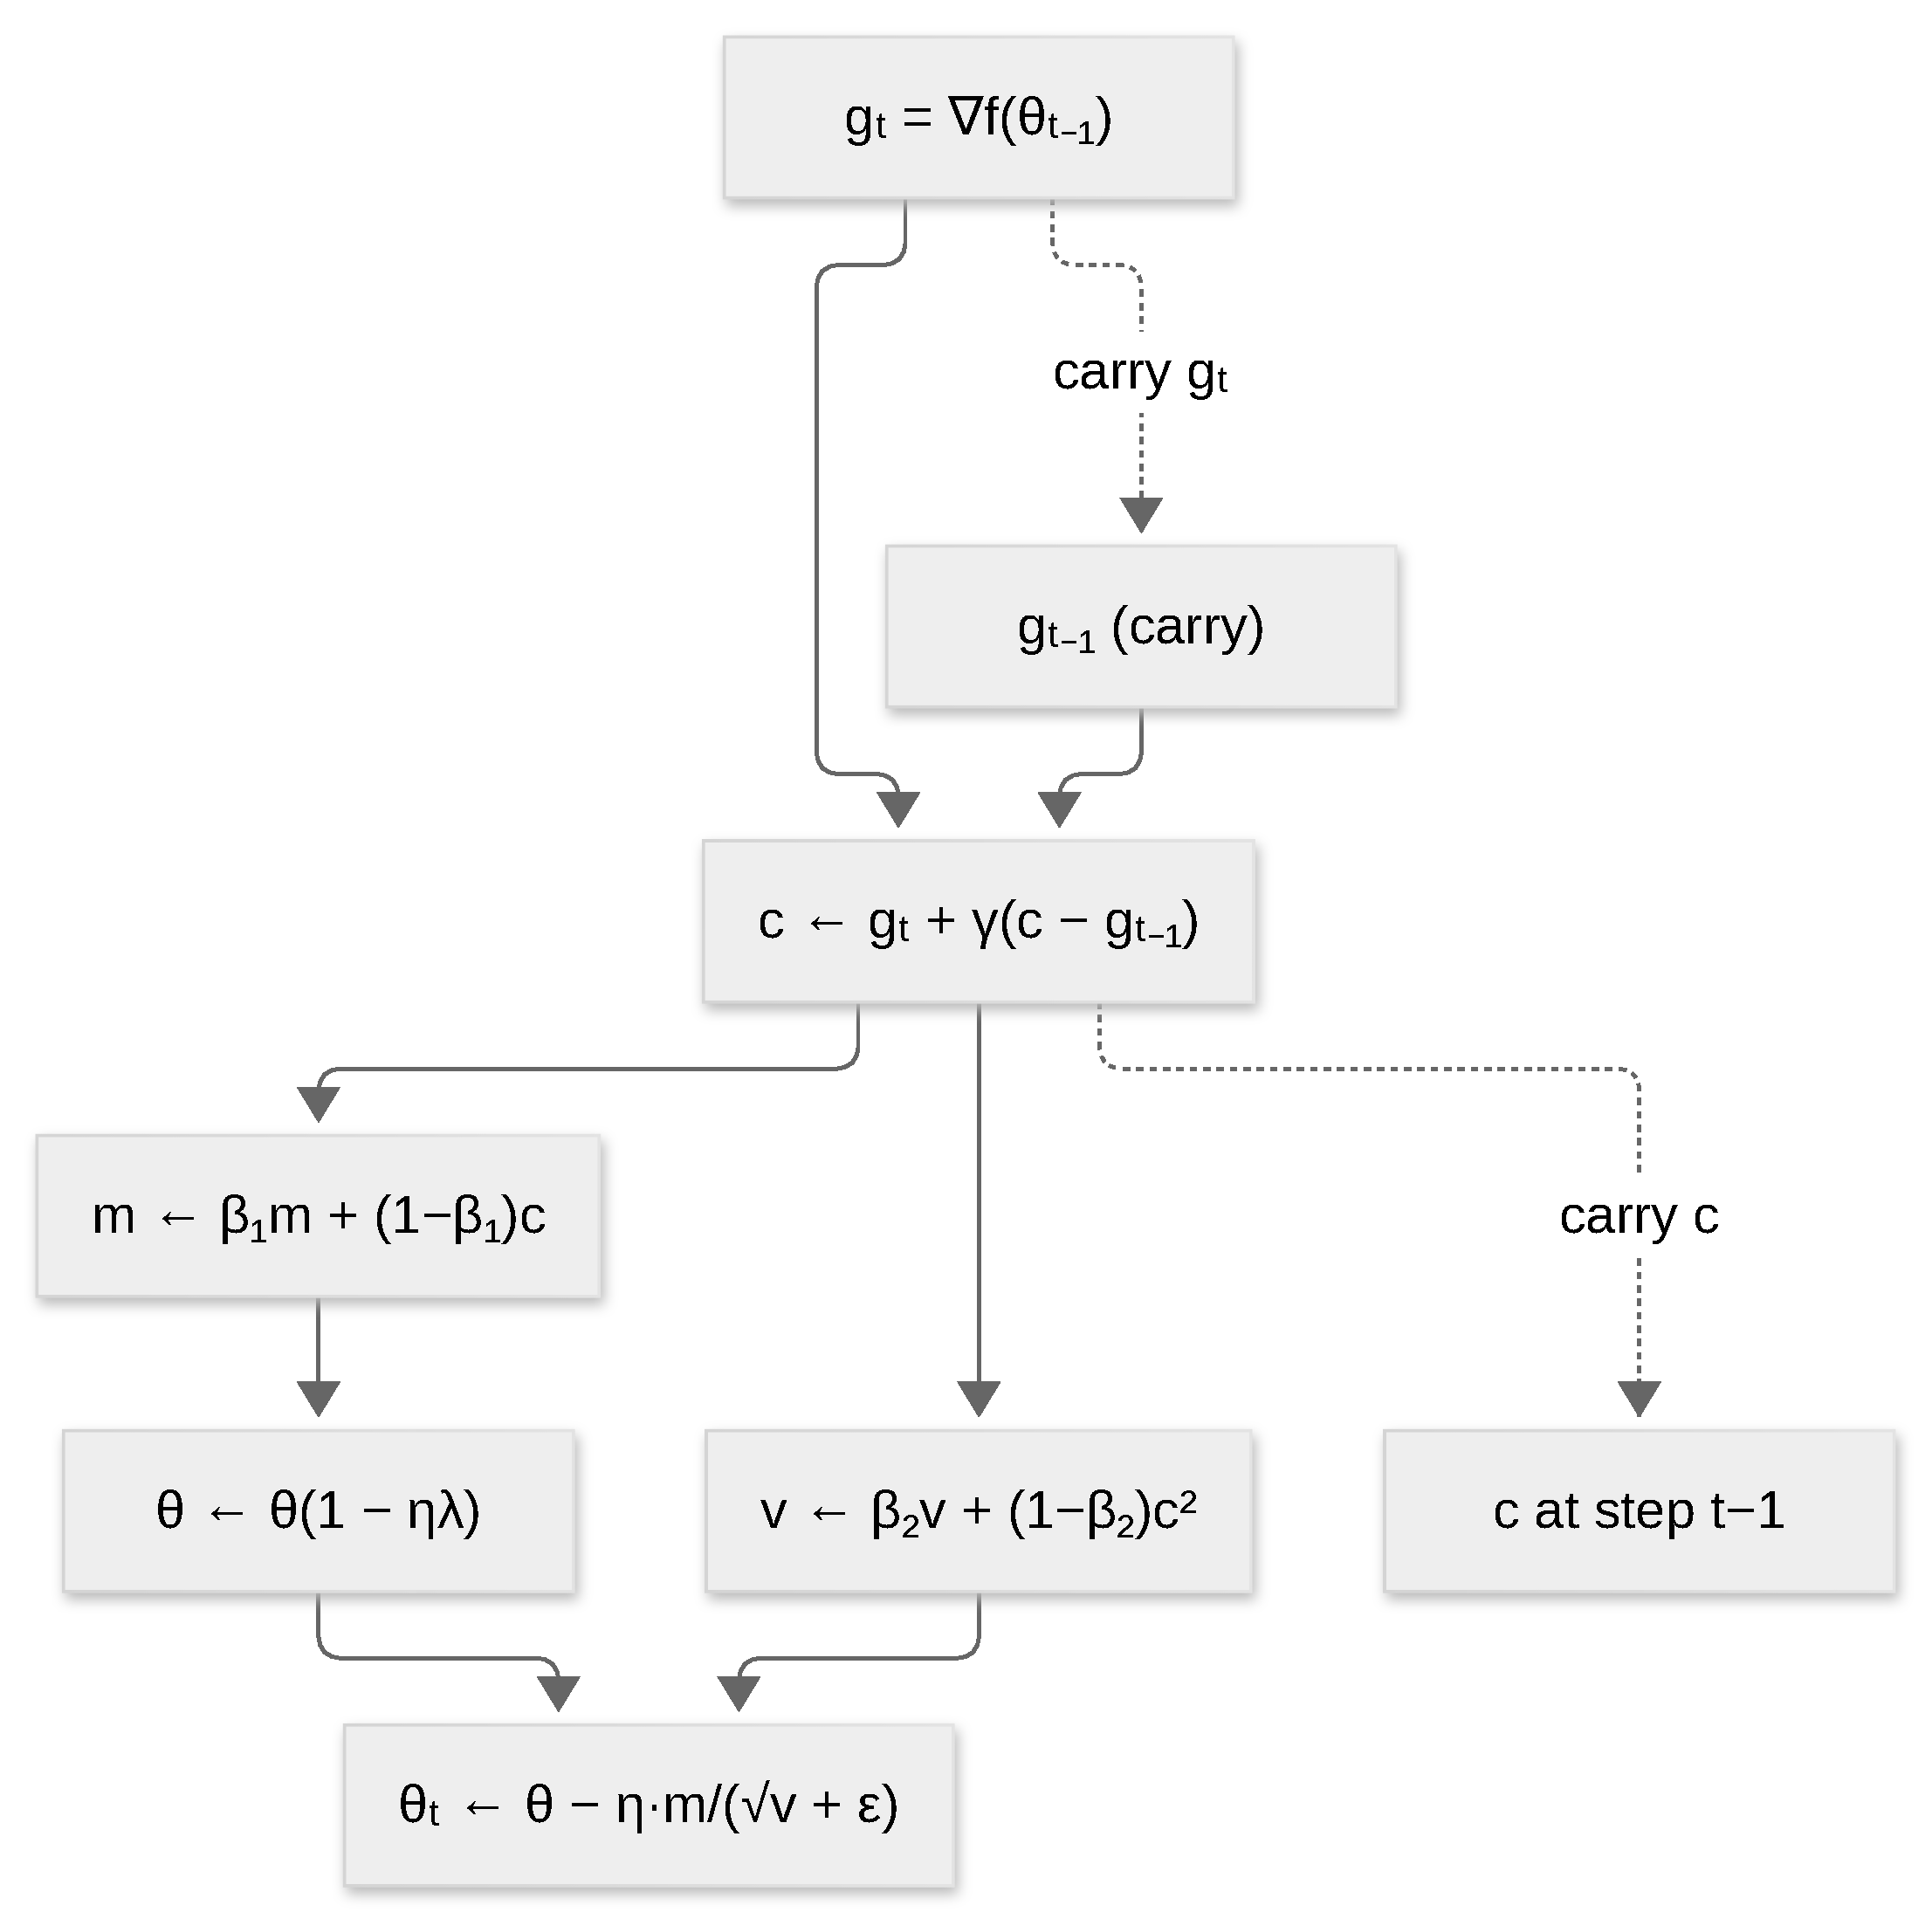
\includegraphics{../paper/figures/optimizers/mars.pdf}}
\caption{Flujo por paso de MARS: una estimación recursiva de gradiente con varianza reducida que alimenta los momentos de primer y segundo orden estilo Adam.}
\label{fig:opt-mars}
\end{figure}
MARS combina métodos de gradiente precondicionado (ej., AdamW) con \textbf{reducción de varianza} mediante momentum recursivo estocástico escalado. La innovación central es una estimación del gradiente con varianza reducida:
\begin{align}
c_t &= g_t + \gamma(c_{t-1} - g_{t-1}) \quad\text{(estimación recursiva tipo SVRG)} \\
m_t &= \beta_1 m_{t-1} + (1-\beta_1)c_t \\
v_t &= \beta_2 v_{t-1} + (1-\beta_2)c_t^2 \\
\theta_{t+1} &= \theta_t - \eta\frac{m_t}{\sqrt{v_t}+\epsilon}
\end{align}
donde $\gamma \in [0.01, 0.1]$ controla cuánta información de gradiente histórico se retiene. El gradiente con varianza reducida $c_t$ actúa como un filtro de ruido implícito, amplificando las direcciones de señal consistentes y amortiguando el ruido contradictorio.

\begin{algorithm}[H]
\caption{MARS (Haciendo Brillar las Tasas de Aprendizaje Adaptativas)}
\label{alg:mars}
\begin{algorithmic}[1]
\Require Parámetros iniciales $\theta_0$, tasa de aprendizaje $\eta$, $\beta_1, \beta_2$, decadencia de peso $\lambda$
\Require Coeficiente de reducción de varianza $\gamma \in [0.01, 0.1]$
\Ensure Parámetros actualizados $\theta_T$
\State Inicializar: $m \gets 0$, $v \gets 0$, $c \gets 0$ (gradiente con varianza reducida), $g_{-1} \gets 0$
\For{$t = 1, 2, \ldots, T$}
    \State $g_t \gets \nabla f(\theta_{t-1})$
    \State Reducción de varianza: $c \gets g_t + \gamma(c - g_{t-1})$
    \State $m \gets \beta_1 m + (1-\beta_1) c$
    \State $v \gets \beta_2 v + (1-\beta_2) c^2$
    \If{decadencia\_de\_peso $> 0$}
        \State $\theta_{t-1} \gets \theta_{t-1}(1 - \eta\lambda)$
    \EndIf
    \State $\theta_t \gets \theta_{t-1} - \eta (m / (\sqrt{v} + \epsilon))$
    \State $g_{t-1} \gets g_t$
\EndFor
\Return $\theta_T$
\end{algorithmic}
\end{algorithm}

\paragraph{Contras.}
\begin{itemize}[leftmargin=*]
\item Almacena el gradiente con varianza reducida y el gradiente anterior además de los momentos de Adam.
\item El coeficiente de reducción de varianza $\gamma \in [0.01, 0.1]$ debe ajustarse.
\end{itemize}

\paragraph{Ventajas.}
\begin{itemize}[leftmargin=*]
\item Actúa como un filtro de ruido implícito, amplificando direcciones consistentes y amortiguando el ruido contradictorio.
\item MARS-AdamW supera consistentemente a AdamW por márgenes significativos en el preentrenamiento de GPT-2.
\end{itemize}

\paragraph{Optimizadores Cautelosos (Cautious AdamW, Cautious Lion).}
\begin{figure}[H]
\centering
\fitfigure{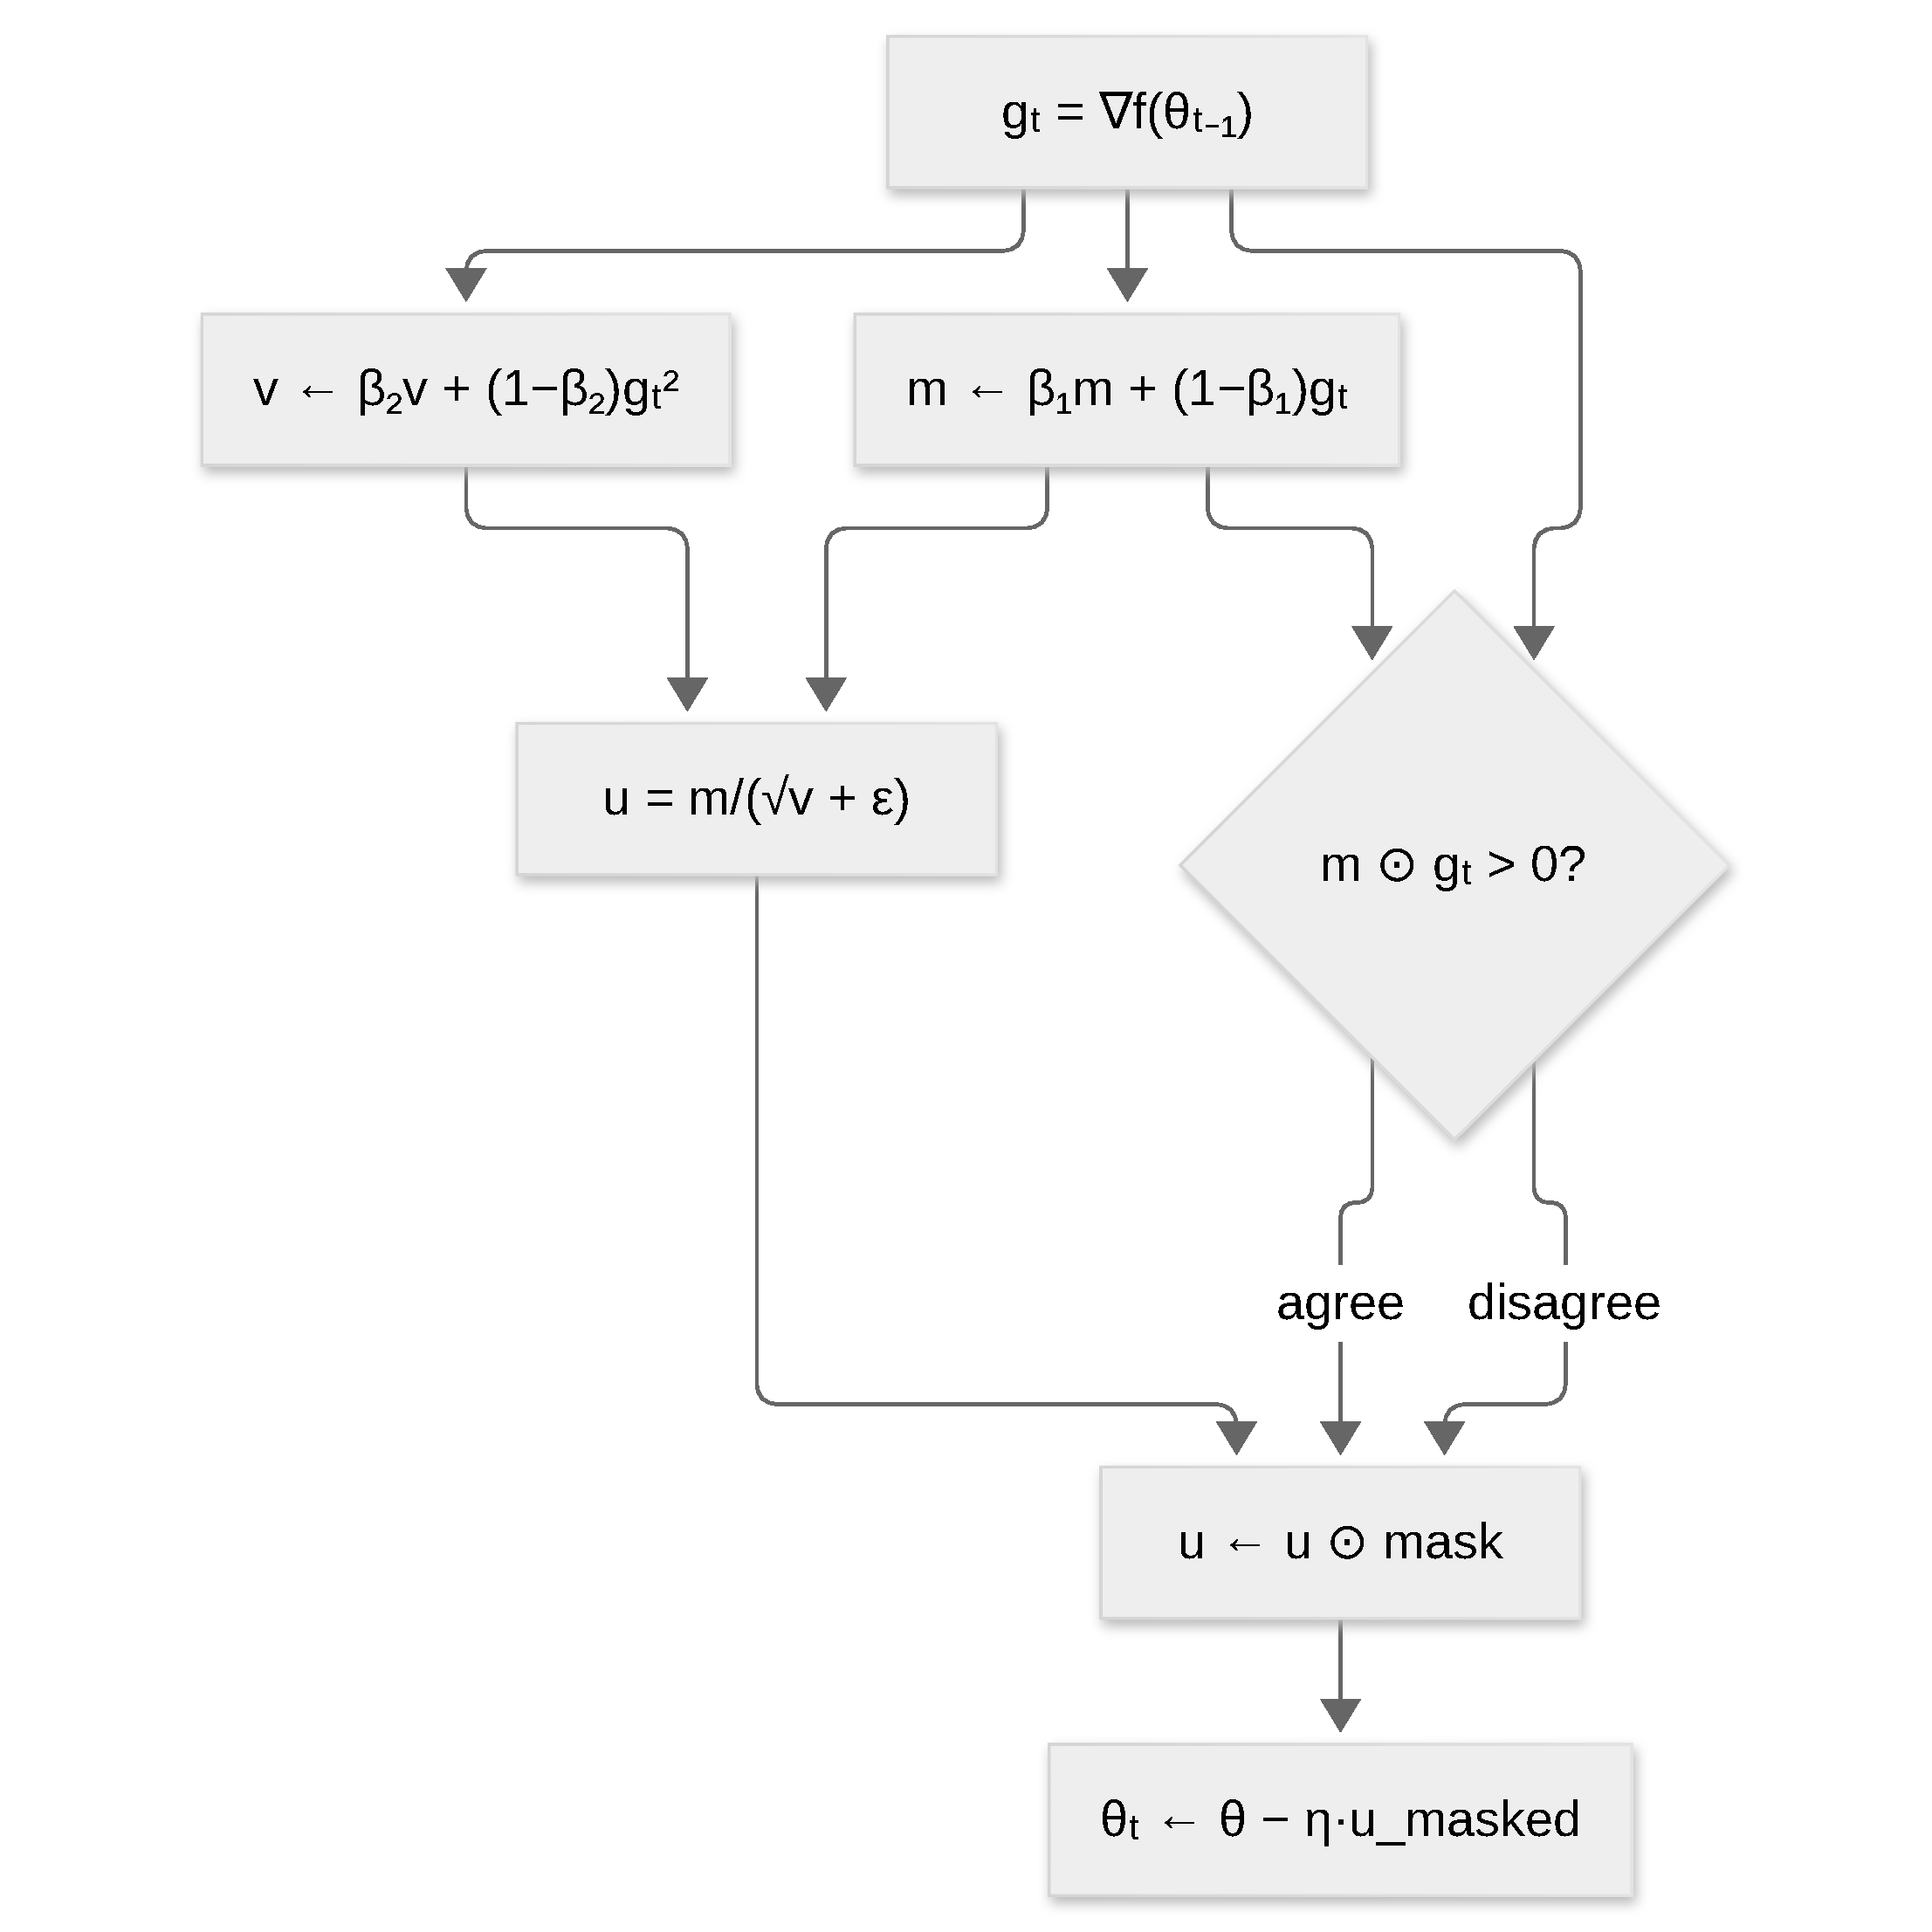
\includegraphics{../paper/figures/optimizers/cautious.pdf}}
\caption{Flujo por paso de Cautious AdamW: una máscara de consenso conserva solo las coordenadas donde momentum y gradiente coinciden.}
\label{fig:opt-cautious}
\end{figure}
El marco Cauteloso aplica una \textbf{modificación de una línea} a cualquier optimizador basado en momentum: enmascarar la actualización de modo que solo se apliquen las dimensiones donde el momentum y la dirección del gradiente coinciden:
\begin{align}
\text{mask}_i &= \begin{cases} 1 & \text{si } m_t[i] \cdot g_t[i] > 0 \quad\text{(acuerdo)} \\ 0 & \text{en caso contrario} \end{cases} \\
u_t &= \left(\frac{m_t}{\sqrt{v_t}+\epsilon}\right) \odot \text{mask} \quad\text{(enmascaramiento elemento a elemento)} \\
\theta_{t+1} &= \theta_t - \eta u_t
\end{align}
La intuición: el momentum $m_t$ estima la dirección del gradiente a partir del historial; el gradiente actual $g_t$ es la señal instantánea. Cuando ambos coinciden, el optimizador está seguro y debe actualizar agresivamente. Cuando discrepan, el optimizador está en conflicto---la tendencia histórica apunta hacia una región que pudo haber sido buena antes, pero la evidencia actual la contradice. Al enmascarar las dimensiones en conflicto, Cauteloso se vuelve más conservador y evita pasos corruptos.

\begin{algorithm}[H]
\caption{Cautious AdamW (Enmascaramiento de Actualización por Consenso)}
\label{alg:cautious}
\begin{algorithmic}[1]
\Require Parámetros iniciales $\theta_0$, tasa de aprendizaje $\eta$, $\beta_1, \beta_2$, decadencia de peso $\lambda$
\Ensure Parámetros actualizados $\theta_T$
\State Inicializar: $m \gets 0$, $v \gets 0$
\For{$t = 1, 2, \ldots, T$}
    \State $g_t \gets \nabla f(\theta_{t-1})$
    \State $m \gets \beta_1 m + (1-\beta_1) g_t$
    \State $v \gets \beta_2 v + (1-\beta_2) g_t^2$
    \State Máscara de consenso: $\text{mask}_i \gets 1$ si $m[i] \cdot g_t[i] > 0$, si no $0$ \Comment{Acuerdo}
    \State Actualización base Adam: $u \gets m / (\sqrt{v} + \epsilon)$
    \State Aplicar máscara: $u_{\text{masked}} \gets u \odot \text{mask}$ \Comment{Elemento a elemento}
    \If{decadencia\_de\_peso $> 0$}
        \State $\theta_{t-1} \gets \theta_{t-1}(1 - \eta\lambda)$
    \EndIf
    \State $\theta_t \gets \theta_{t-1} - \eta u_{\text{masked}}$
\EndFor
\Return $\theta_T$
\end{algorithmic}
\end{algorithm}

\paragraph{Contras.}
\begin{itemize}[leftmargin=*]
\item El enmascaramiento puede descartar actualizaciones útiles cuando momentum y gradiente discrepan temporalmente.
\item Requiere un optimizador base con momentum además de la máscara elemento a elemento.
\end{itemize}

\paragraph{Ventajas.}
\begin{itemize}[leftmargin=*]
\item Modificación de una línea aplicable a cualquier optimizador basado en momentum.
\item Hasta \textbf{1.47$\times$ de aceleración} en el preentrenamiento de Llama y MAE preservando las garantías de convergencia.
\end{itemize}

\subsection{Optimizadores de Lote Grande, Eficientes en Memoria y Sin Tasa de Aprendizaje}
\paragraph{LAMB (Layer-wise Adaptive Moments optimizer for Batch training).}
\begin{figure}[H]
\centering
\fitfigure{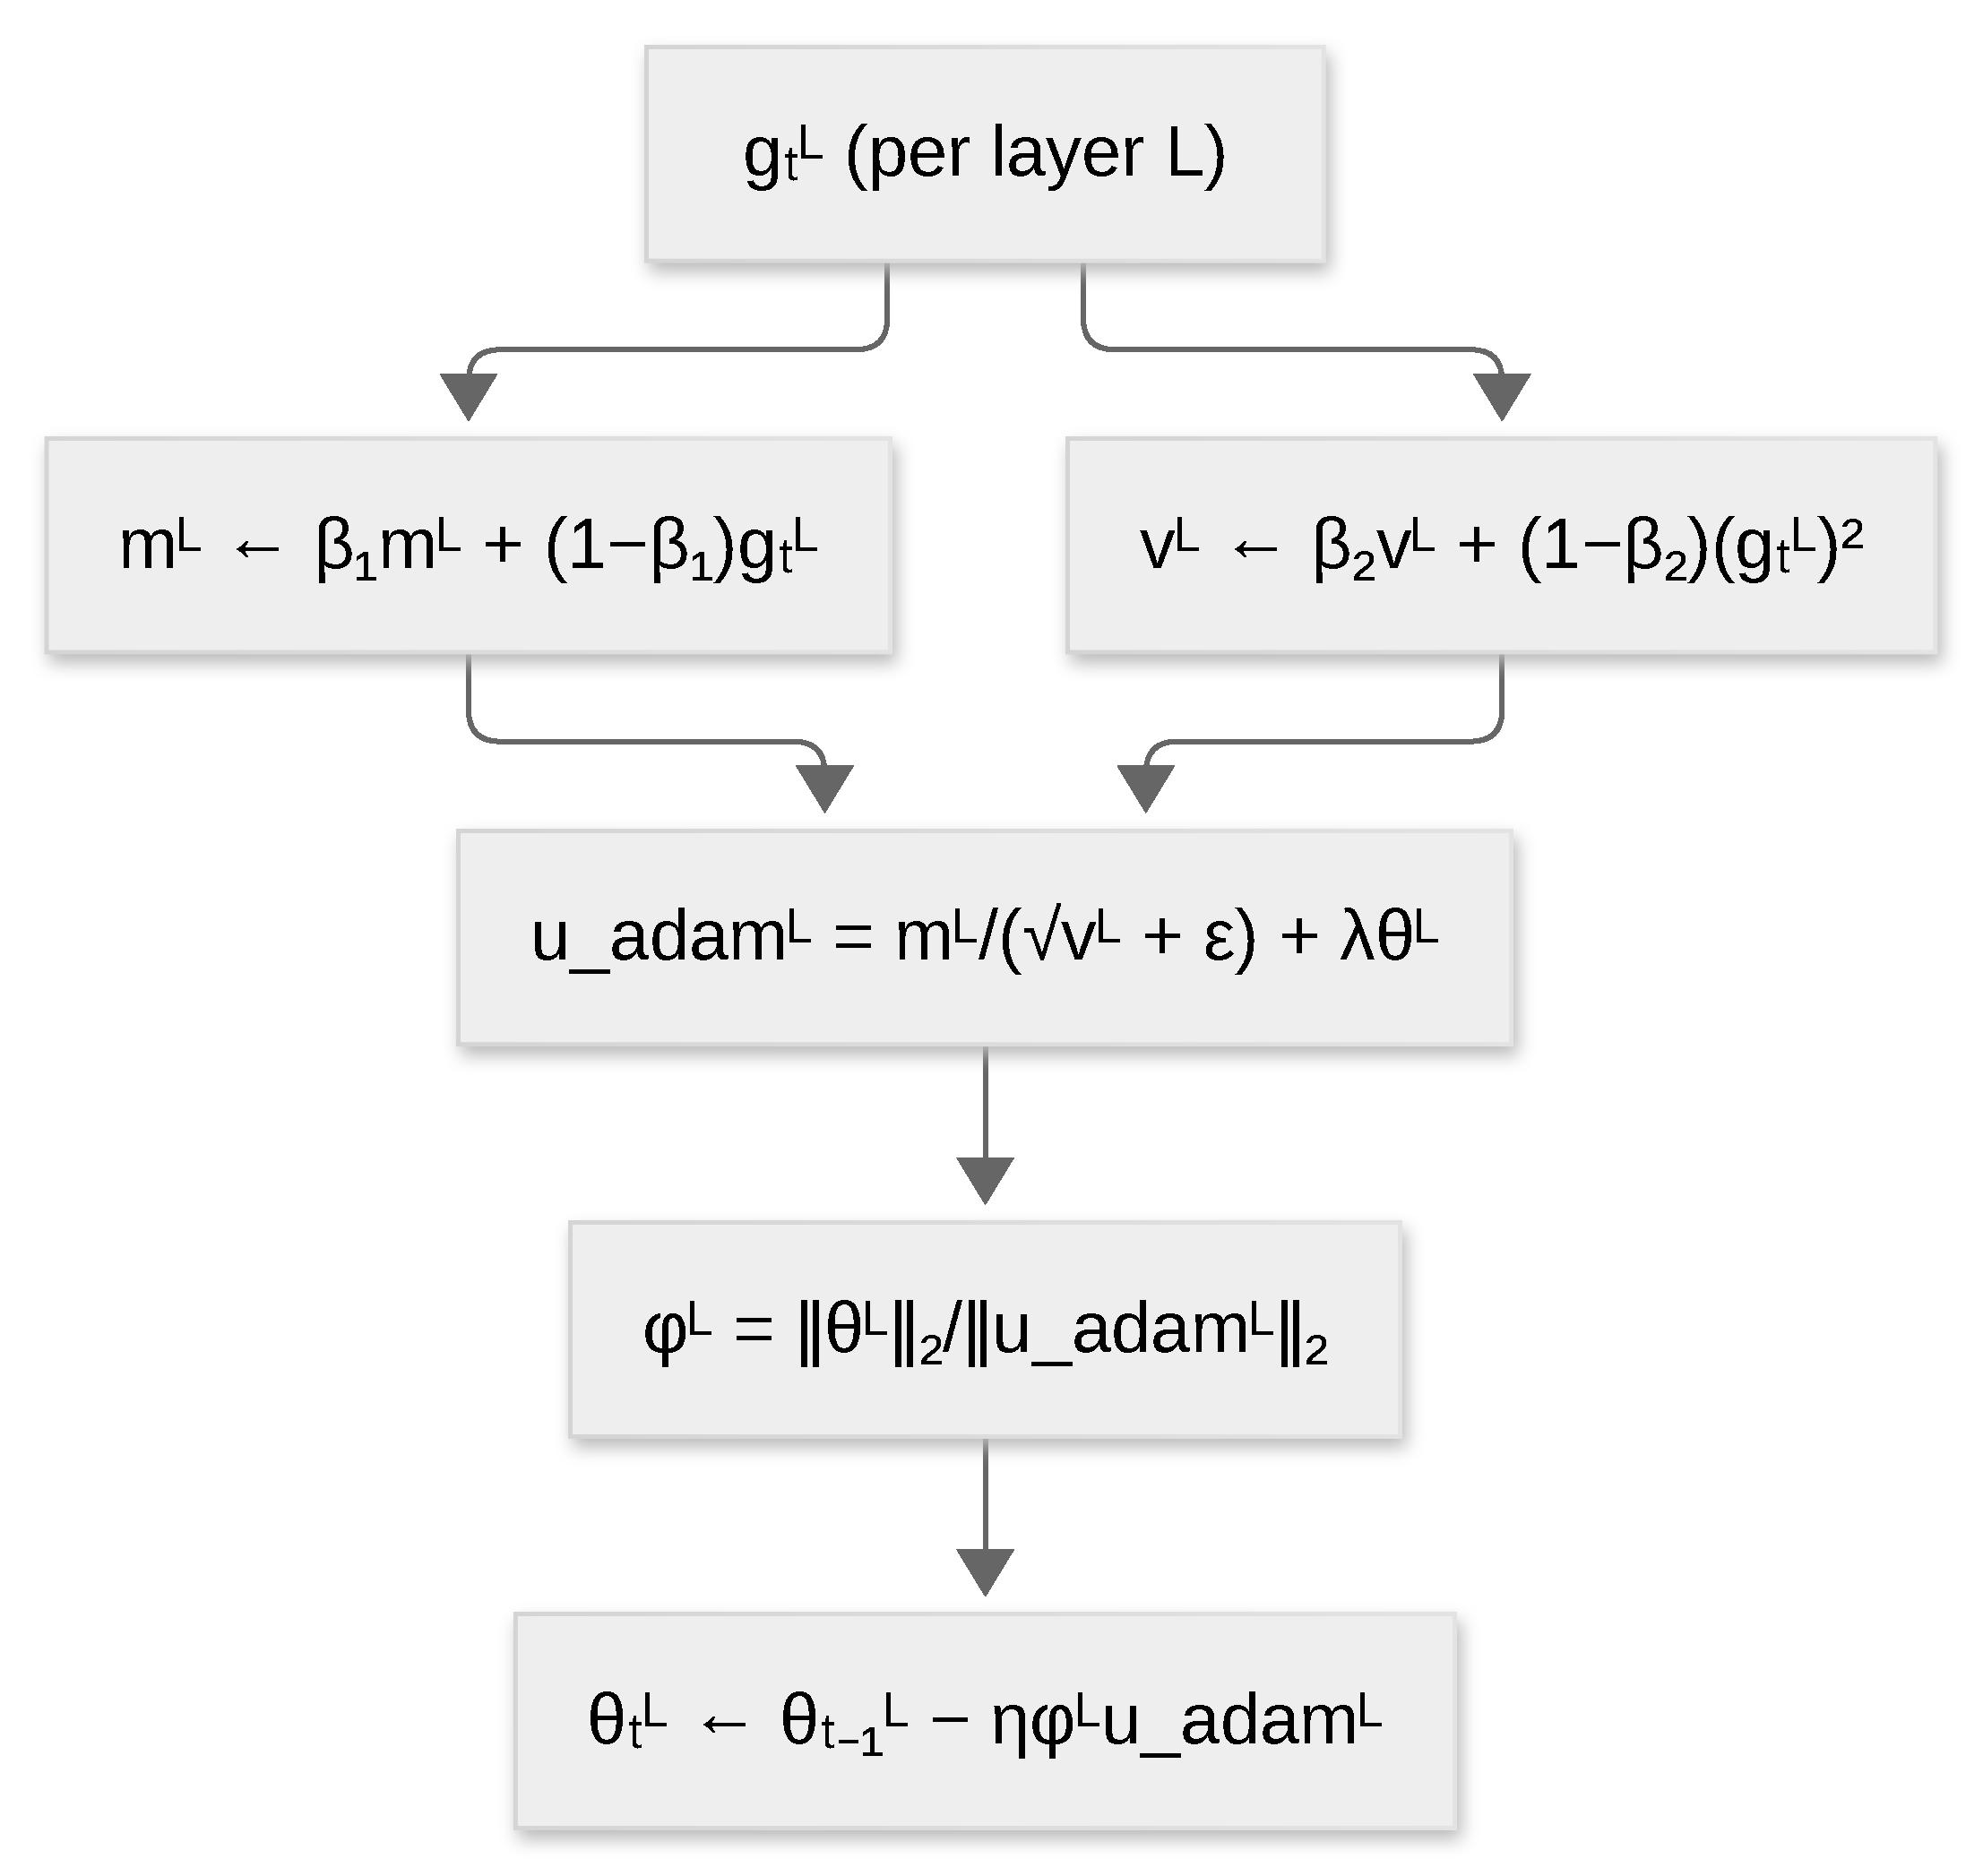
\includegraphics{../paper/figures/optimizers/lamb.pdf}}
\caption{Flujo por paso de LAMB: paso Adam por capas reescalado por la razón de confianza entre las normas de pesos y actualización.}
\label{fig:opt-lamb}
\end{figure}
LAMB extiende Adam con \textbf{escalado de tasa adaptativo por capas} (inspirado en LARS), permitiendo entrenamiento estable con tamaños de lote extremos (e.g., 64K en BERT):
\begin{align}
m_t^L &= \beta_1 m_{t-1}^L + (1-\beta_1)g_t^L \quad\text{(momento de primer orden por capas)} \\
v_t^L &= \beta_2 v_{t-1}^L + (1-\beta_2)(g_t^L)^2 \\
u_{\text{adam}}^L &= \frac{m_t^L}{\sqrt{v_t^L}+\epsilon} + \lambda\theta_{t-1}^L \quad\text{(paso adaptativo base con decaimiento)} \\
\phi^L &= \frac{\|\theta_{t-1}^L\|_2}{\|u_{\text{adam}}^L\|_2} \quad\text{(razón de confianza: normalización por capas)} \\
\theta_t^L &= \theta_{t-1}^L - \eta \cdot \phi^L \cdot u_{\text{adam}}^L
\end{align}
La \textbf{razón de confianza} $\phi^L = \|\theta^L\|_2 / \|u_{\text{adam}}^L\|_2$ normaliza el paso de actualización efectivo en relación con la magnitud de los pesos. En lotes muy grandes, el ruido estocástico del gradiente puede superar a la señal, desestabilizando las tasas de aprendizaje por capas. Al escalar las actualizaciones proporcionalmente a las normas de los pesos, LAMB asegura cambios relativos en lugar de absolutos, evitando que actualizaciones pequeñas y seguras en vectores grandes dominen.

\begin{algorithm}[H]
\caption{LAMB (Layer-wise Adaptive Moments optimizer for Batch training)}
\label{alg:lamb}
\begin{algorithmic}[1]
\Require Parámetros iniciales $\theta_0$, tasa de aprendizaje $\eta$, $\beta_1, \beta_2$, decaimiento de pesos $\lambda$
\Ensure Parámetros actualizados $\theta_T$
\State Inicializar: Para cada capa $L$: $m^L \gets 0$, $v^L \gets 0$
\For{$t = 1, 2, \ldots, T$}
    \For{cada capa $L$}
        \State $g_t^L \gets \nabla f(\theta_t^L)$
        \State $m^L \gets \beta_1 m^L + (1-\beta_1) g_t^L$
        \State $v^L \gets \beta_2 v^L + (1-\beta_2) (g_t^L)^2$
        \State Adam base: $u_{\text{adam}}^L \gets m^L / (\sqrt{v^L} + \epsilon)$
        \If{weight\_decay $> 0$}
            \State $u_{\text{adam}}^L \gets u_{\text{adam}}^L + \lambda \theta_{t-1}^L$
        \EndIf
        \State Razón de confianza: $\phi^L \gets \|\theta_{t-1}^L\|_2 / \|u_{\text{adam}}^L\|_2$ si ambos son no nulos, sino $1$
        \State $\theta_t^L \gets \theta_{t-1}^L - \eta \phi^L u_{\text{adam}}^L$
    \EndFor
\EndFor
\Return $\theta_T$
\end{algorithmic}
\end{algorithm}

\paragraph{Contras.}
\begin{itemize}[leftmargin=*]
\item La contabilidad de normas por capas y el cálculo de la razón de confianza añaden sobrecarga por paso.
\item La razón de confianza es inestable cuando las normas de capa o de actualización son cercanas a cero.
\end{itemize}

\paragraph{Ventajas.}
\begin{itemize}[leftmargin=*]
\item Permite entrenamiento estable con tamaños de lote extremos (e.g., 64K en BERT).
\item Preserva los beneficios de generalización de lotes pequeños mientras escala el lote.
\end{itemize}

\paragraph{Schedule-Free AdamW.}
\begin{figure}[H]
\centering
\fitfigure{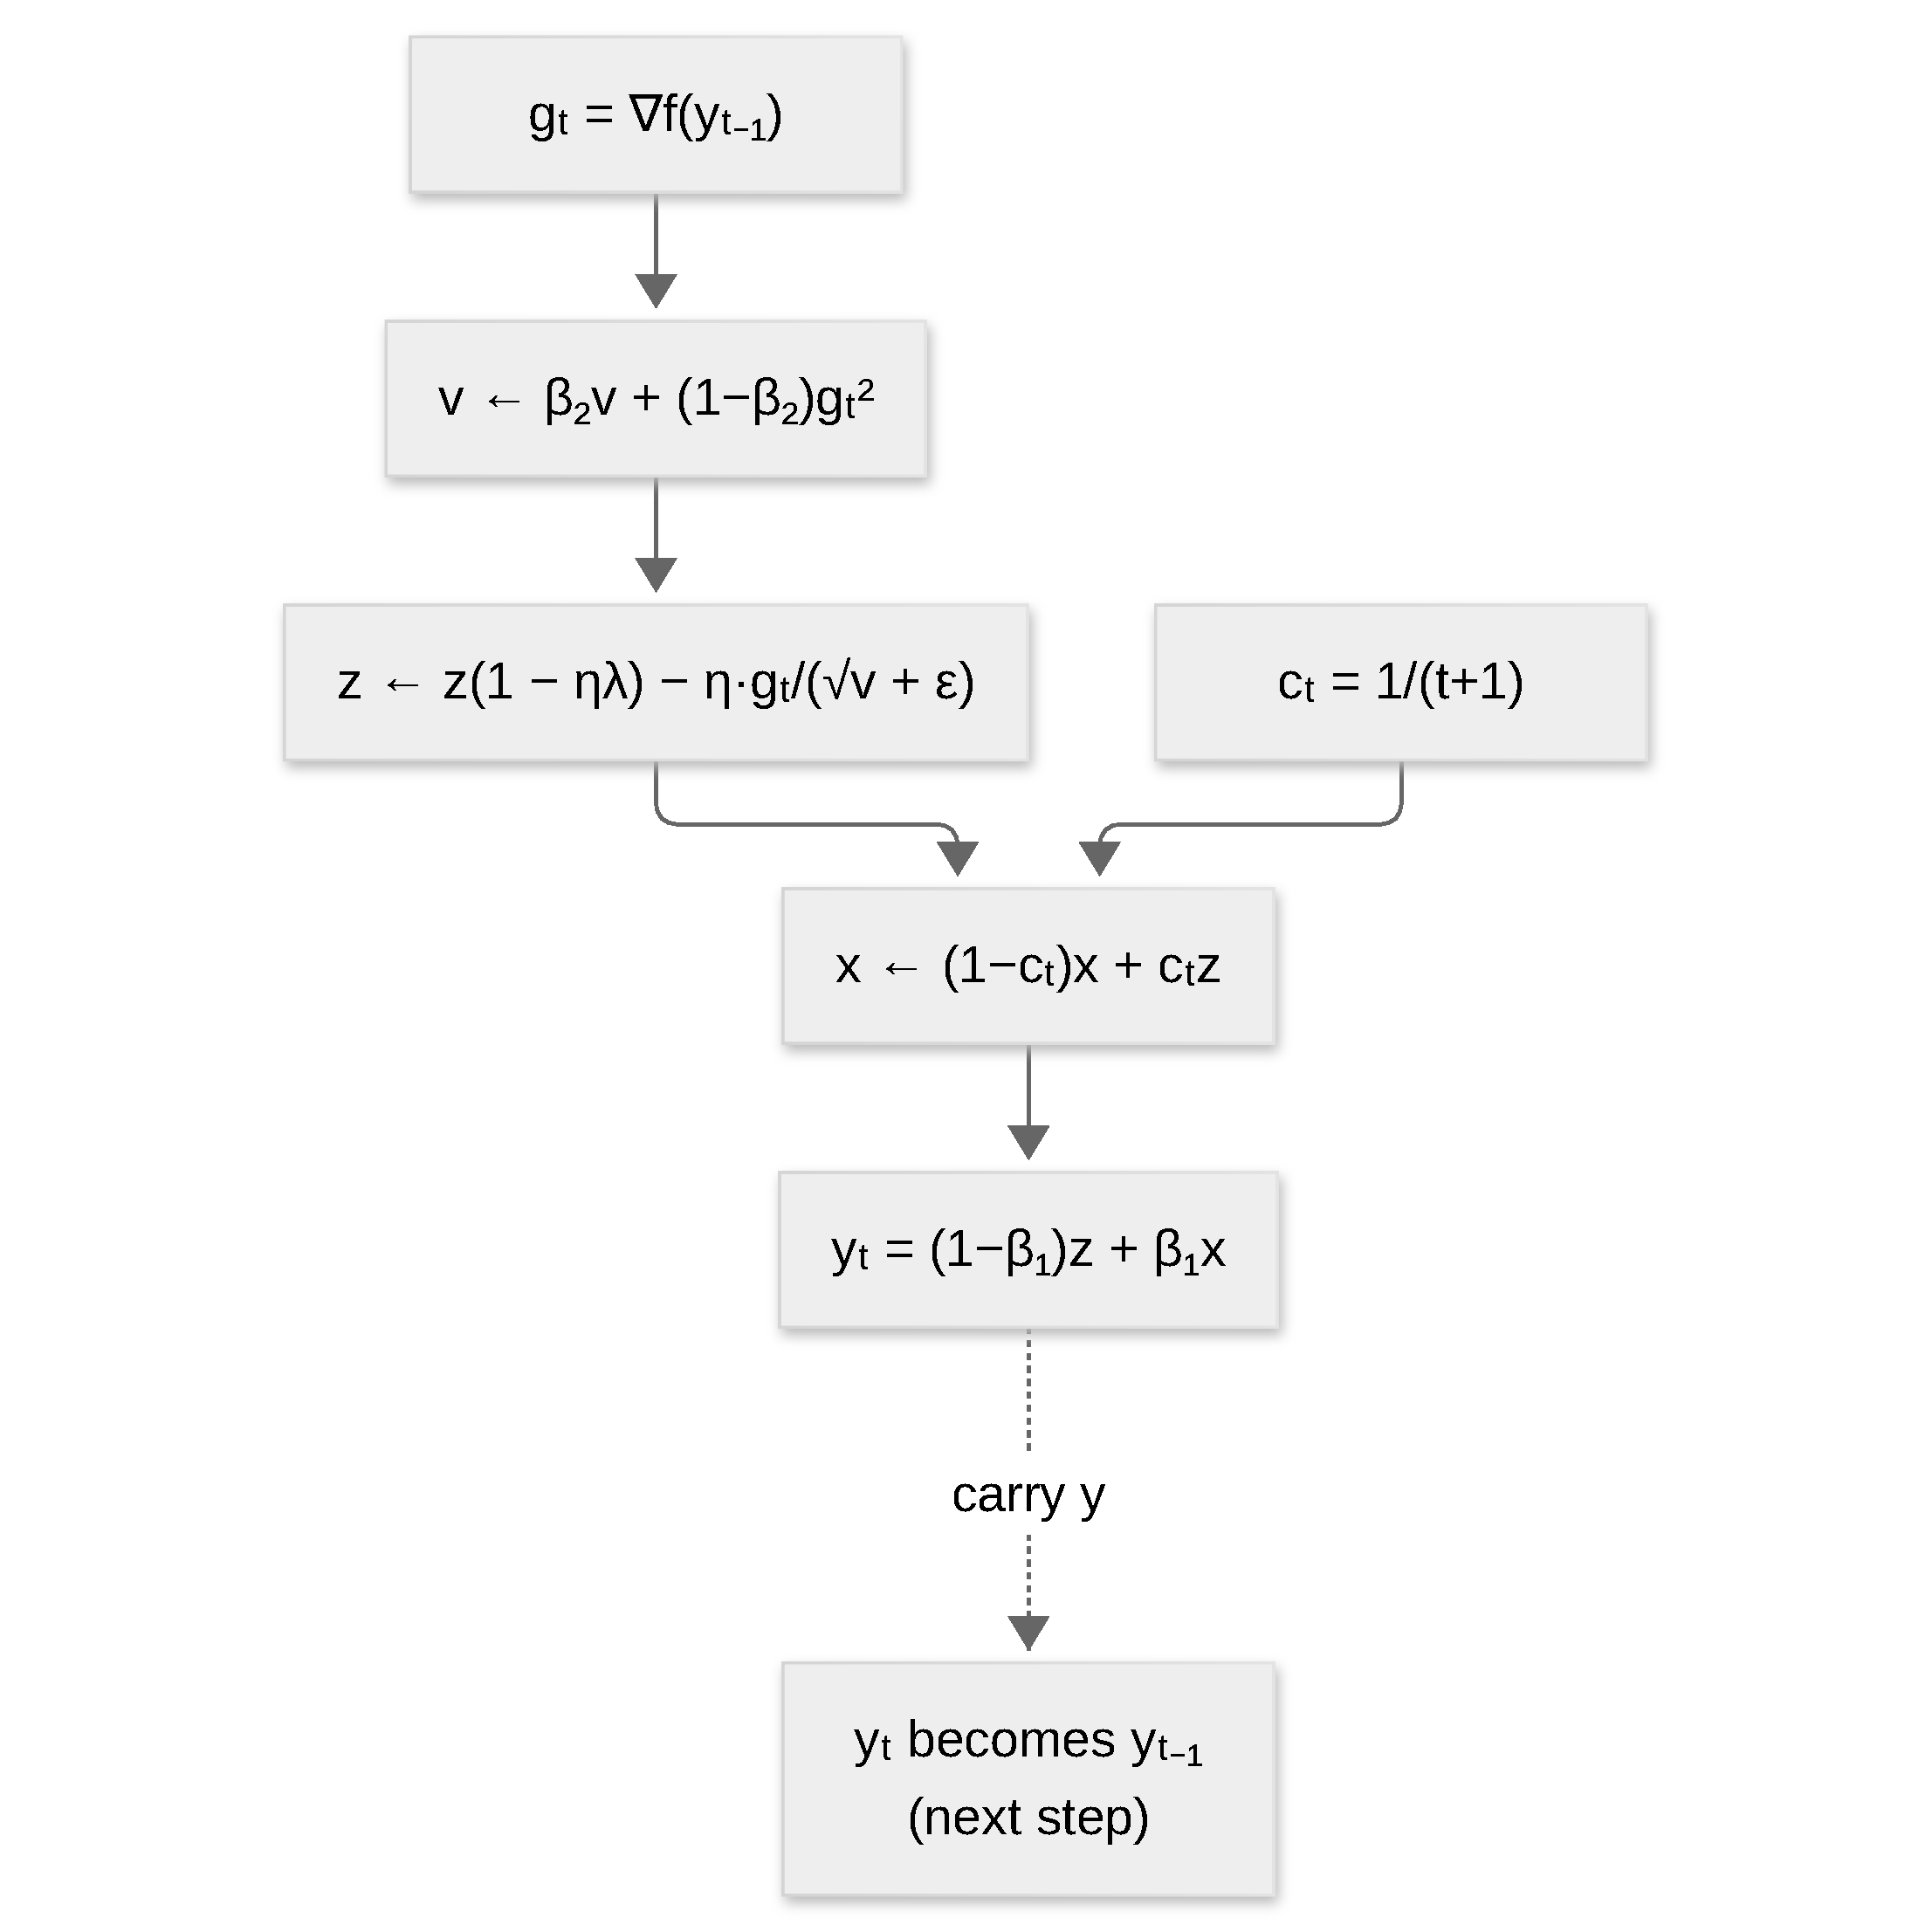
\includegraphics{../paper/figures/optimizers/schedulefree.pdf}}
\caption{Flujo por paso de Schedule-Free AdamW: flujo de exploración $z$, promedio de iteraciones $x$ y punto de interpolación $y$, con promediado implícito $1/(t+1)$.}
\label{fig:opt-schedulefree}
\end{figure}
Los métodos Schedule-Free eliminan el diseño explícito de programación de la receta de optimización. El algoritmo mantiene dos flujos de parámetros: $z_t$ (exploración) y $x_t$ (promedio suavizado):
\begin{align}
v_t &= \beta_2 v_{t-1} + (1-\beta_2)g_t^2 \quad\text{(varianza)} \\
z_t &= z_{t-1}(1-\eta\lambda) - \eta\frac{g_t}{\sqrt{v_t}+\epsilon} \quad\text{(paso adaptativo con decaimiento)} \\
c_t &= \frac{1}{t+1} \quad\text{(coeficiente de promediado, decrece con el tiempo)} \\
x_t &= (1-c_t)x_{t-1} + c_t z_t \quad\text{(promediado de iteraciones)} \\
y_t &= (1-\beta)z_t + \beta x_t \quad\text{(interpolación para el punto de evaluación)}
\end{align}
El coeficiente de promediado $c_t = 1/(t+1)$ implementa una programación de tasa de aprendizaje implícita sin especificar explícitamente el número total de pasos $T$. Este marco unifica la programación y el promediado de iteraciones: el algoritmo explora mediante $z_t$ mientras acumula dirección estable mediante $x_t$. El punto de evaluación $y_t$ (usado para el cómputo del gradiente) interpola entre exploración y estabilidad.

\begin{algorithm}[H]
\caption{Schedule-Free AdamW}
\label{alg:schedulefree}
\begin{algorithmic}[1]
\Require Parámetros iniciales $\theta_0$, tasa de aprendizaje $\eta$ (fija), $\beta_1, \beta_2$, decaimiento de pesos $\lambda$
\Ensure Parámetros actualizados $\theta_T$ o promediado $x_T$
\State Inicializar: $z \gets \theta_0$ (exploración), $x \gets \theta_0$ (promedio), $v \gets 0$, $t \gets 0$
\For{$t = 1, 2, \ldots, T$}
    \State $g_t \gets \nabla f(y_{t-1})$ (gradiente en el punto de interpolación)
    \State $v \gets \beta_2 v + (1-\beta_2) g_t^2$ \Comment{Varianza}
    \State Decaimiento de pesos sobre $z$: $z \gets z(1 - \eta\lambda)$
    \State $z \gets z - \eta g_t / (\sqrt{v} + \epsilon)$ \Comment{Paso adaptativo sobre el gradiente crudo}
    \State $c_t \gets 1 / (t+1)$ \Comment{Coeficiente de promediado}
    \State $x \gets (1-c_t) x + c_t z$ \Comment{Promediado de iteraciones}
    \State $y_t \gets (1-\beta_1) z + \beta_1 x$ \Comment{Interpolación para la siguiente evaluación}
\EndFor
\Return $x_T$ o $y_T$
\end{algorithmic}
\end{algorithm}

\paragraph{Contras.}
\begin{itemize}[leftmargin=*]
\item Mantiene dos flujos de parámetros ($z$ y $x$) y requiere manejar explícitamente el punto de evaluación.
\item Su comportamiento difiere de las líneas base con programación, lo que complica las comparaciones.
\end{itemize}

\paragraph{Ventajas.}
\begin{itemize}[leftmargin=*]
\item Elimina la programación explícita de la tasa de aprendizaje y su hiperparámetro de pasos totales.
\item Convergencia de última generación en optimización convexa, aprendizaje profundo a gran escala y aprendizaje por refuerzo.
\end{itemize}

\paragraph{Adafactor.}
\begin{figure}[H]
\centering
\fitfigure{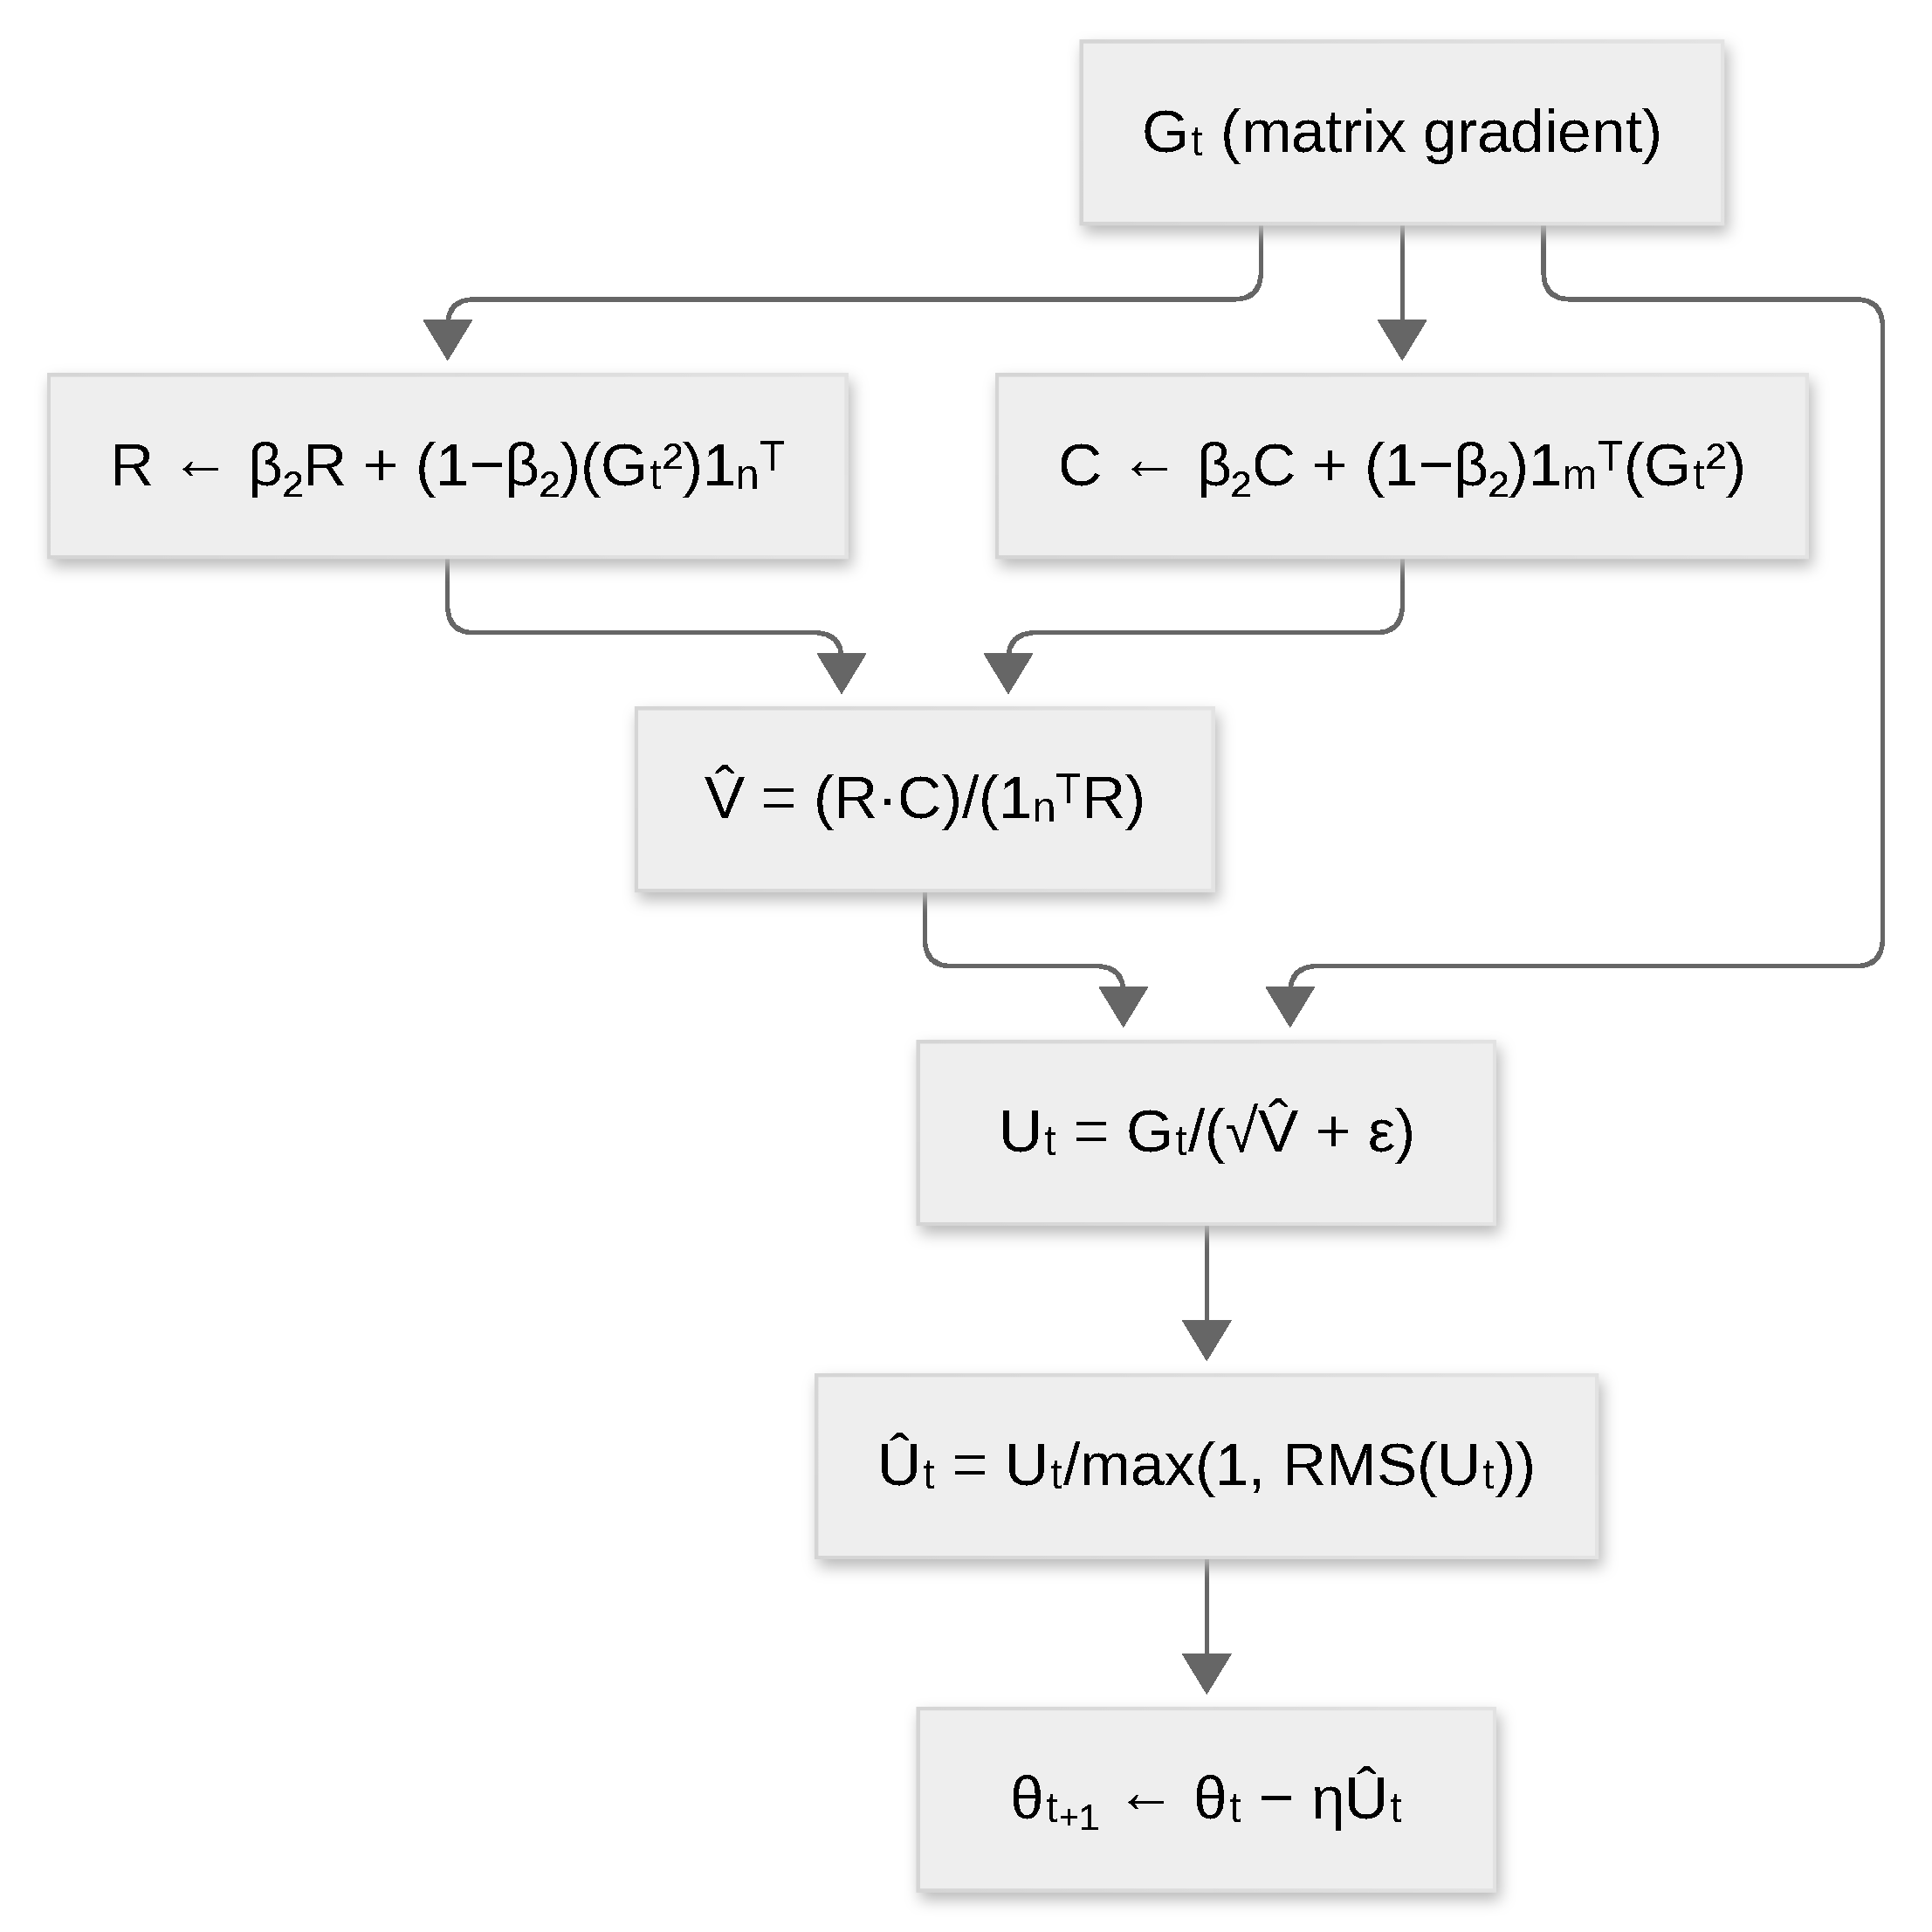
\includegraphics{../paper/figures/optimizers/adafactor.pdf}}
\caption{Flujo por paso de Adafactor: acumuladores factorizados de segundo momento por filas y columnas, reconstrucción mediante producto exterior y recorte RMS.}
\label{fig:opt-adafactor}
\end{figure}
Adafactor reduce la memoria del optimizador \textbf{factorizando} estadísticas de segundo momento para parámetros con forma de matriz, almacenando solo acumuladores de filas y columnas en lugar de estados de varianza densos. Para una matriz de gradiente $G_t \in \mathbb{R}^{m \times n}$:
\begin{align}
R_t &= \beta_2 R_{t-1} + (1-\beta_2)(G_t^2) \mathbf{1}_n^T \quad\text{(varianza por filas)} \\
C_t &= \beta_2 C_{t-1} + (1-\beta_2) \mathbf{1}_m^\top (G_t^2) \quad\text{(varianza por columnas)} \\
\hat{V}_t &= \frac{R_t C_t}{\mathbf{1}_n^\top R_t} \quad\text{(varianza reconstruida mediante producto exterior)} \\
U_t &= \frac{G_t}{\sqrt{\hat{V}_t}+\epsilon} \quad\text{(paso adaptativo normalizado)} \\
\hat{U}_t &= \frac{U_t}{\max(1, \text{RMS}(U_t))} \quad\text{(recorte de estabilidad)}
\end{align}

\begin{algorithm}[H]
\caption{Adafactor (Estadísticas de Segundo Momento Factorizadas)}
\label{alg:adafactor}
\begin{algorithmic}[1]
\Require Matriz de gradiente $G_t \in \mathbb{R}^{m \times n}$, tasa de aprendizaje $\eta$, $\beta_2 \approx 0.999$
\Ensure Parámetros actualizados $\theta_T$
\State Inicializar: Acumuladores de fila $R \gets \epsilon \mathbf{1}^T_m$, Columna $C \gets \epsilon \mathbf{1}_n$
\For{$t = 1, 2, \ldots, T$}
    \State $G_t \gets \nabla f(\theta_t)$ (gradiente matricial)
    \State $R \gets \beta_2 R + (1-\beta_2) (G_t^2) \mathbf{1}_n^T$ \Comment{Productos internos por filas}
    \State $C \gets \beta_2 C + (1-\beta_2) \mathbf{1}_m^\top (G_t^2)$ \Comment{Productos internos por columnas}
    \State Varianza reconstruida: $\hat{V} \gets (R \cdot C) / (\mathbf{1}_n^\top R)$ \Comment{Mediante producto exterior}
    \State Paso adaptativo normalizado: $U_t \gets G_t / (\sqrt{\hat{V}} + \epsilon)$
    \State Recorte RMS por fila: $\hat{U}_t \gets U_t / \max(1, \text{RMS}(U_t))$
    \State $\theta_{t+1} \gets \theta_t - \eta \hat{U}_t$
\EndFor
\Return $\theta_T$
\end{algorithmic}
\end{algorithm}

\paragraph{Contras.}
\begin{itemize}[leftmargin=*]
\item La varianza factorizada es una aproximación y puede ser inestable en algunas tareas.
\item Menor expresividad de optimización en comparación con Adam completo.
\end{itemize}

\paragraph{Ventajas.}
\begin{itemize}[leftmargin=*]
\item La memoria baja de $O(n_{\text{params}})$ a $O(\sqrt{n_{\text{params}}})$ para parámetros matriciales.
\item Más atractivo cuando la VRAM está dominada por el estado del optimizador en lugar de las activaciones.
\end{itemize}

\paragraph{GaLore (Gradient Low-Rank Projection).}
\begin{figure}[H]
\centering
\fitfigure{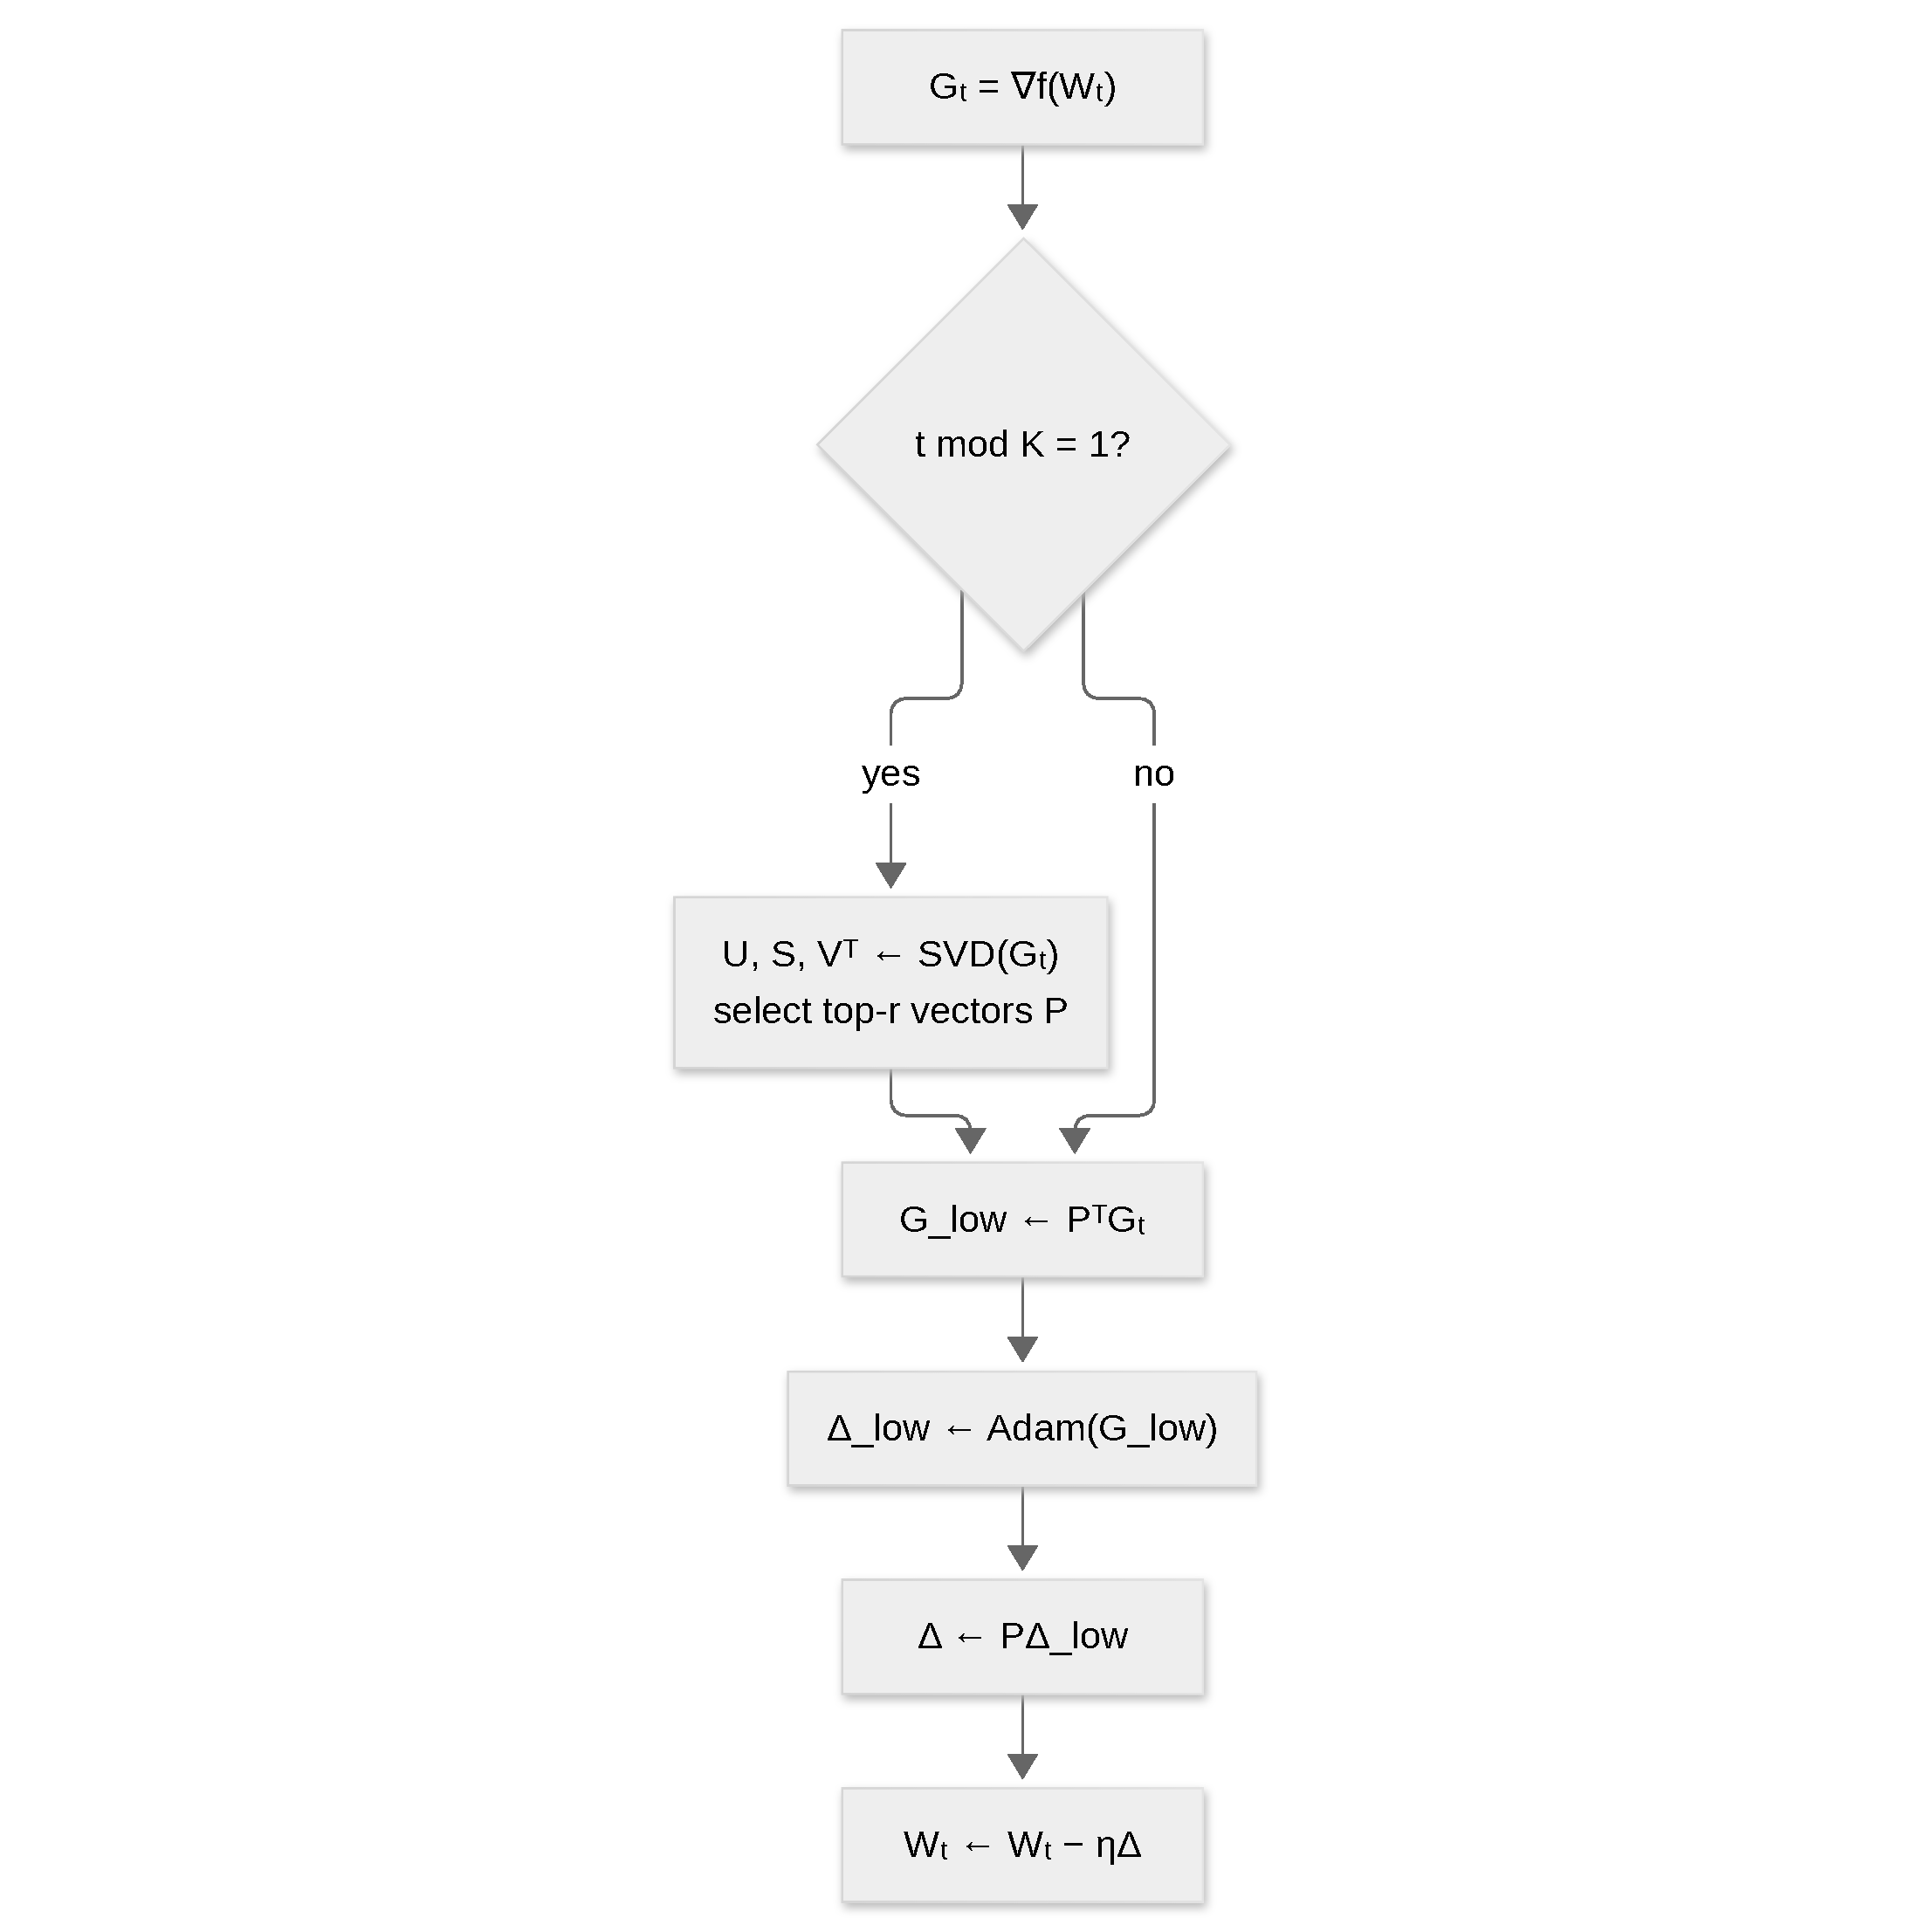
\includegraphics{../paper/figures/optimizers/galore.pdf}}
\caption{Flujo por paso de GaLore: proyección SVD periódica del gradiente a un subespacio de bajo rango, Adam en ese subespacio y reconstrucción.}
\label{fig:opt-galore}
\end{figure}
GaLore proyecta gradientes 2D en un subespacio de bajo rango antes de la optimización, reduciendo la memoria del estado del optimizador mientras mantiene el escalado adaptativo del paso. Para una matriz de parámetros 2D $W \in \mathbb{R}^{m \times n}$:
\begin{align}
U, S, V &= \text{SVD}(G_t) \quad\text{(calcular descomposición singular)} \\
P &\in \mathbb{R}^{n \times r} \quad\text{o} \quad P^\top \in \mathbb{R}^{r \times m} \quad\text{(seleccionar los $r$ vectores singulares superiores)} \\
G_{\text{low}} &= P^\top G_t \quad\text{(proyectar al espacio de bajo rango)} \\
\Delta_{\text{low}} &= \text{Adam}(G_{\text{low}}) \quad\text{(optimizar en el espacio comprimido)} \\
\Delta &= P \Delta_{\text{low}} \quad\text{(reconstruir en el espacio original)}
\end{align}
Al proyectar en un subespacio de rango $r$ (típicamente $r \ll \min(m,n)$), el estado del optimizador se reduce de $O(mn)$ a $O(r(m+n))$ para parámetros 2D. Este enfoque complementario de ahorro de memoria es especialmente relevante cuando el modelo es demasiado grande para el estado completo del optimizador.

\begin{algorithm}[H]
\caption{GaLore (Gradient Low-Rank Projection)}
\label{alg:galore}
\begin{algorithmic}[1]
\Require Matriz de parámetros 2D $W \in \mathbb{R}^{m \times n}$, tasa de aprendizaje $\eta$, rango $r \ll \min(m,n)$
\Ensure Parámetros actualizados $\theta_T$
\State Inicializar: Estado de Adam en el espacio de bajo rango (si es variante de rango 2)
\For{$t = 1, 2, \ldots, T$}
    \State $G_t \gets \nabla f(W_t)$
    \If{$t \mod K = 1$}  \Comment{SVD periódico}
        \State $U_t, S_t, V_t^\top \gets \text{SVD}(G_t)$ (completa o delgada)
        \State Seleccionar proyección: $P \gets U_t[:, :r]$ o $P \gets V_t[:, :r]$
    \EndIf
    \State Proyectar gradiente: $G_{\text{low}} \gets P^\top G_t$ (o $G_t P^\top$ para proyección derecha)
    \State Ejecutar Adam en bajo rango: $\Delta_{\text{low}} \gets \text{Adam}(G_{\text{low}})$
    \State Reconstruir en espacio original: $\Delta \gets P \Delta_{\text{low}}$ (o $\Delta_{\text{low}} P^\top$)
    \State $W_t \gets W_t - \eta \Delta$
\EndFor
\Return $\theta_T$
\end{algorithmic}
\end{algorithm}

\paragraph{Contras.}
\begin{itemize}[leftmargin=*]
\item El SVD periódico añade cómputo e introduce un intervalo de actualización de la proyección que ajustar.
\item La proyección de bajo rango puede descartar información del gradiente.
\end{itemize}

\paragraph{Ventajas.}
\begin{itemize}[leftmargin=*]
\item El estado del optimizador se reduce de $O(mn)$ a $O(r(m+n))$ para parámetros 2D.
\item Funciona sinérgicamente con otras técnicas y ha mostrado resultados sólidos en modelos de miles de millones de parámetros.
\end{itemize}

\paragraph{APOLLO, APOLLO-Mini, y Q-APOLLO.}
\begin{figure}[H]
\centering
\fitfigure{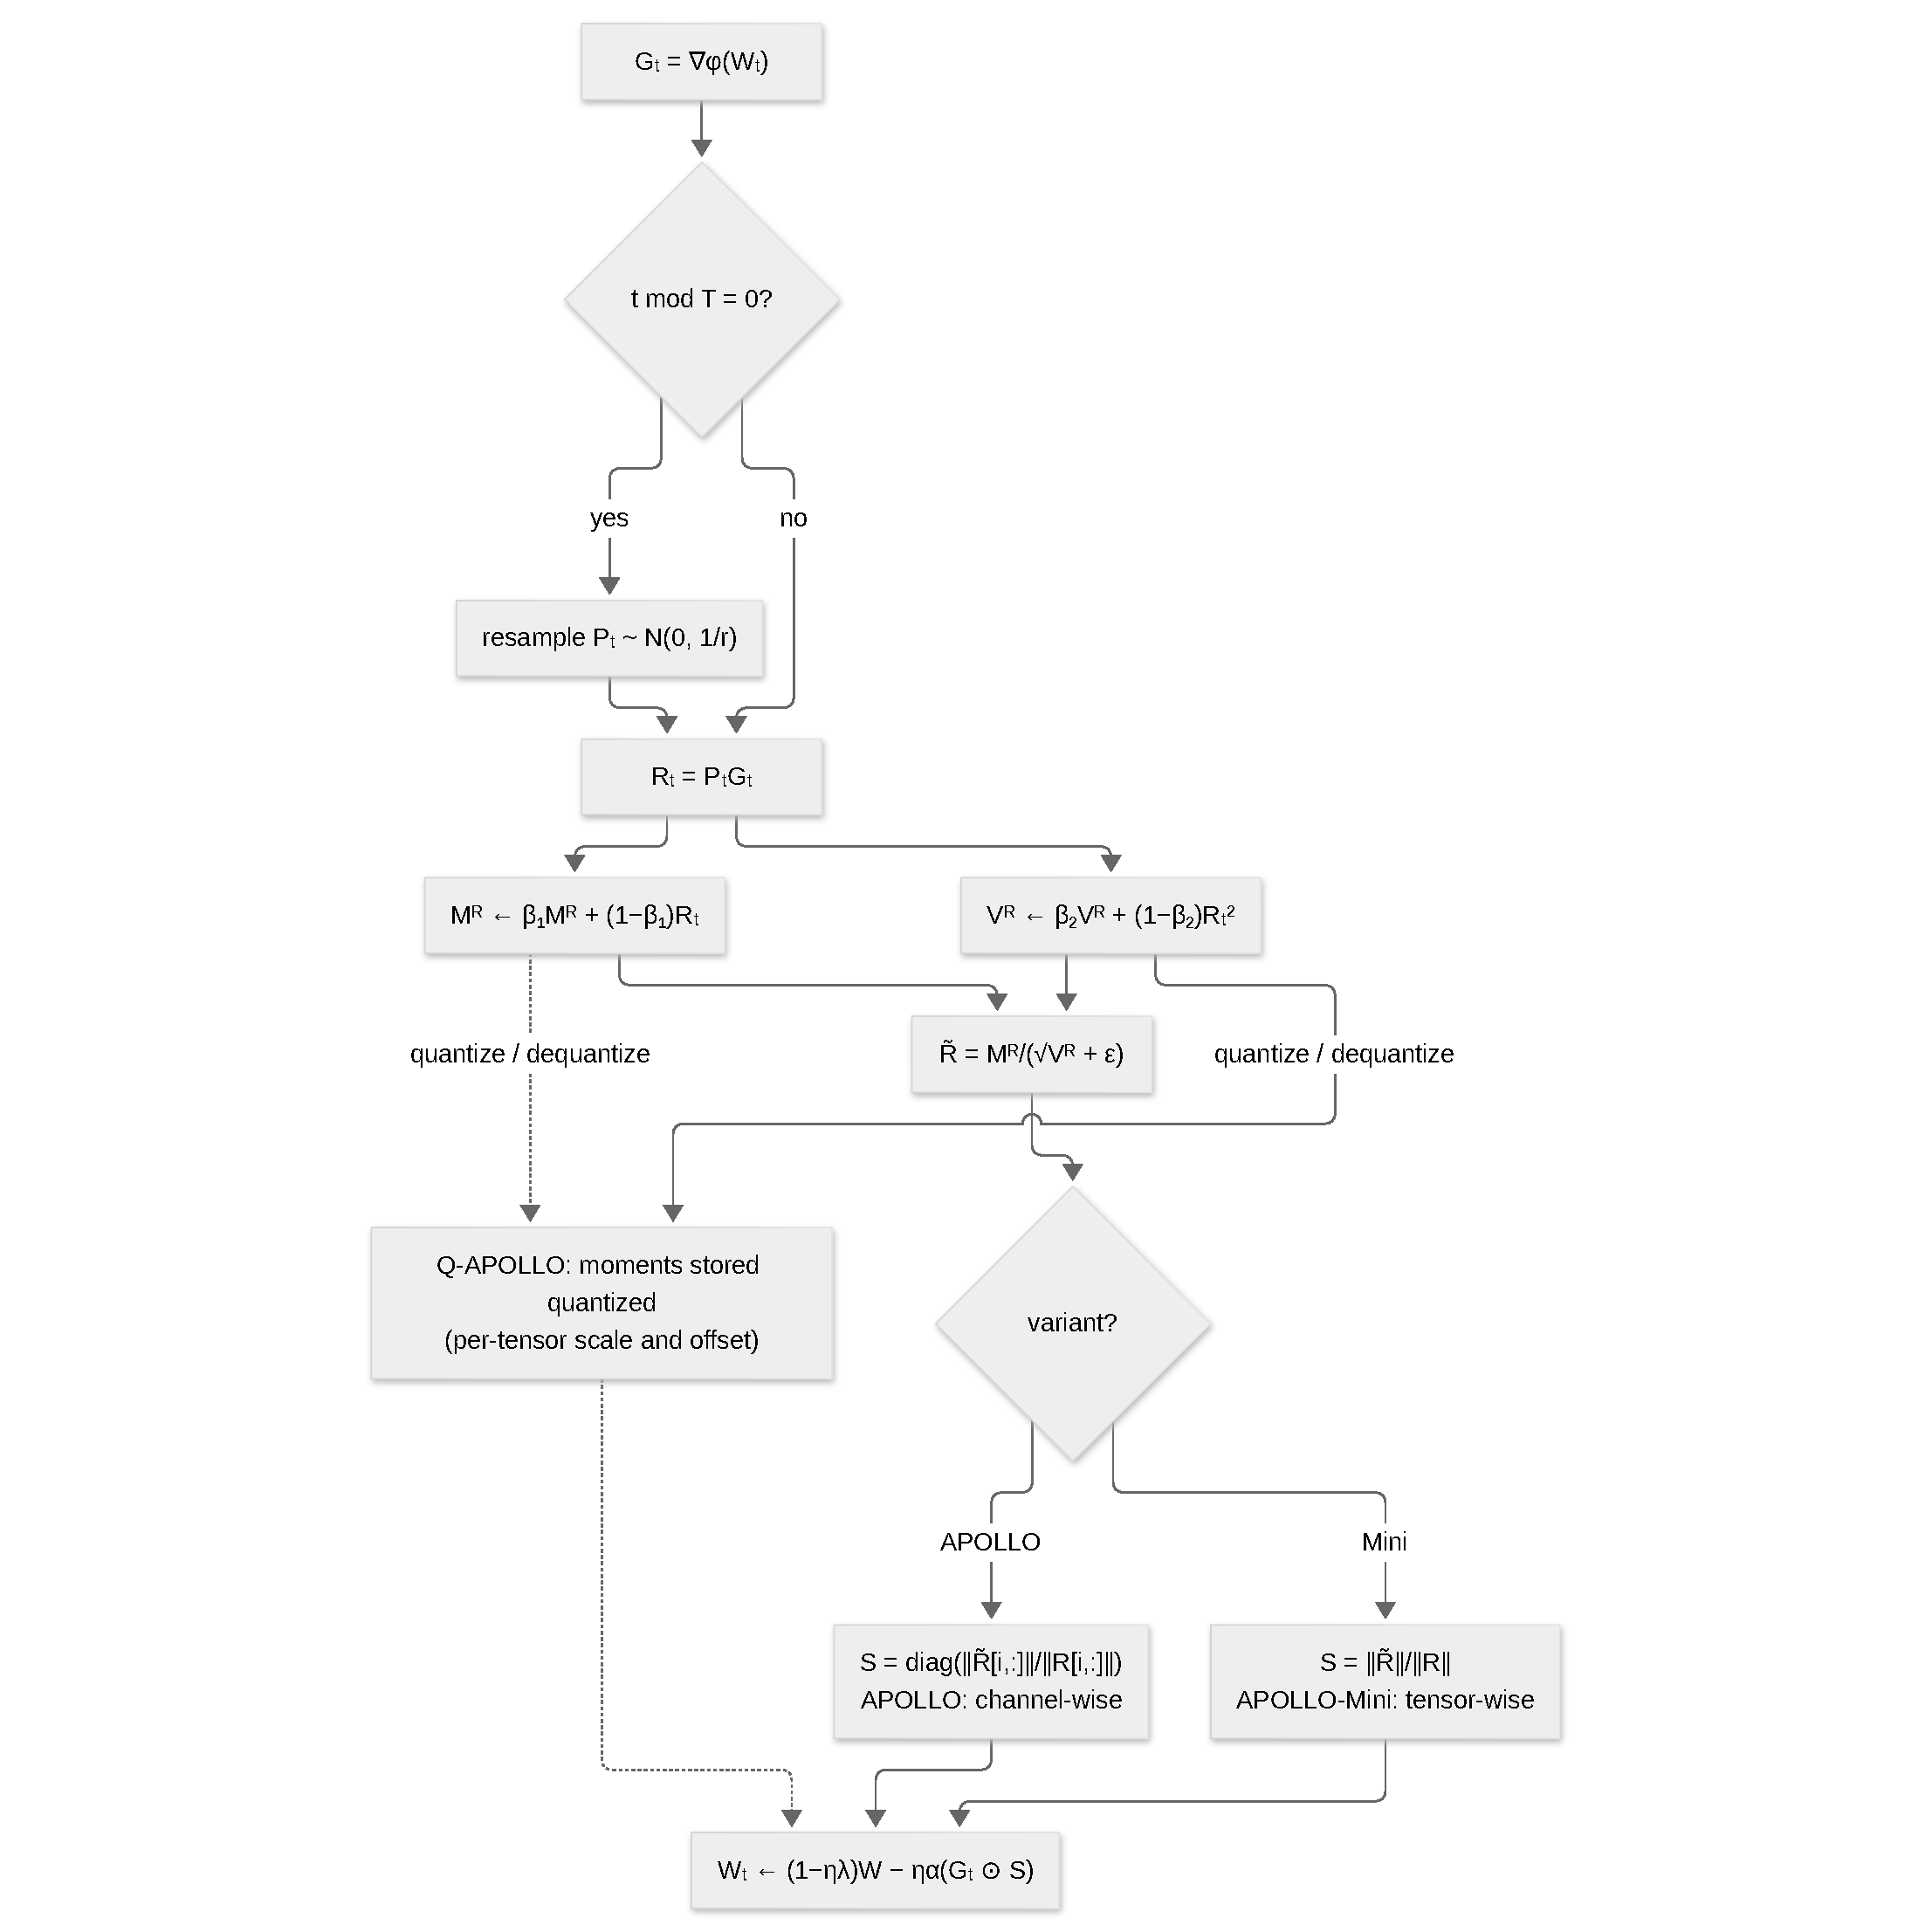
\includegraphics{../paper/figures/optimizers/apollo.pdf}}
\caption{Flujo por paso de la familia APOLLO: momentos proyectados gaussianos, escalado estructurado del gradiente (por canales en APOLLO, escalar en APOLLO-Mini) y estado cuantizado en Q-APOLLO.}
\label{fig:opt-apollo}
\end{figure}
La familia APOLLO \citep{zhu2025apollosgdlikememoryadamwlevel} parte de la observación de que el denominador elemento a elemento de AdamW puede \textbf{transformarse en una actualización estructurada de la tasa de aprendizaje}. En lugar de almacenar momentos densos para cada entrada de parámetro, APOLLO proyecta un gradiente matricial $G_t \in \mathbb{R}^{m \times n}$ en un subespacio aleatorio compacto y rastrea momentos estilo Adam allí:
\begin{align}
R_t &= P_t G_t \quad\text{o}\quad R_t = G_t P_t^\top \\
M_t^R &= \beta_1 M_{t-1}^R + (1-\beta_1)R_t \\
V_t^R &= \beta_2 V_{t-1}^R + (1-\beta_2)R_t^2 \\
\widetilde{R}_t &= \frac{M_t^R}{\sqrt{V_t^R}+\epsilon}
\end{align}
El estado proyectado \emph{no} se expande de vuelta a una actualización densa de bajo rango como en los métodos basados en SVD. En su lugar, APOLLO estima un tensor de escalado estructurado $S_t$ en el espacio original. En la variante estándar de APOLLO, ese escalado es \textbf{por canales}: cada fila o canal recibe su propia razón de norma. En APOLLO-Mini, el escalado se reduce a un único escalar \textbf{por tensor}, correspondiente al caso extremo de rango 1 descrito en el artículo. La actualización de parámetros resultante es, por tanto, similar a Adam en adaptación pero mucho más cercana a SGD en costo de estado:
\[
W_t \gets (1-\eta\lambda)W_{t-1} - \eta\,\alpha\,(G_t \odot S_t)
\]
donde $\alpha$ es el factor de escala adicional usado para estabilizar variantes altamente comprimidas.

\begin{algorithm}[H]
\caption{APOLLO / APOLLO-Mini Escalado de Gradiente Estructurado}
\label{alg:apollo-family}
\begin{algorithmic}[1]
\Require Matriz de pesos $W \in \mathbb{R}^{m \times n}$ con $m \le n$, tasa de aprendizaje $\eta$, factor de escala $\alpha$, tasas de decaimiento $(\beta_1, \beta_2)$, decaimiento de pesos $\lambda$, rango $r$, intervalo de actualización de proyección $T$
\Ensure Parámetros actualizados $W_T$
\State Inicializar momentos proyectados: $M^R \gets 0$, $V^R \gets 0$, paso $t \gets 0$
\Repeat
    \State Calcular gradiente: $G_t \gets \nabla_W \phi(W_t)$
    \If{$t \bmod T = 0$}
        \State Muestrear proyector gaussiano $P_t \sim \mathcal{N}(0, 1/r)$ con una semilla nueva
    \EndIf
    \State Proyectar gradiente: $R_t \gets P_t G_t$ \Comment{o $G_t P_t^\top$ según la disposición}
    \State Actualizar momentos proyectados AdamW: $M_t^R, V_t^R \gets \text{AdamWState}(R_t; \beta_1, \beta_2)$
    \State Normalizar estado proyectado: $\widetilde{R}_t \gets M_t^R / (\sqrt{V_t^R}+\epsilon)$
    \If{APOLLO}
        \State $S_t \gets \operatorname{diag}(s_1^R, \ldots, s_m^R)$, donde $s_i^R = \|\widetilde{R}_t[i,:]\|_2 / \|R_t[i,:]\|_2$
    \Else
        \State $S_t \gets s_t^R$, donde $s_t^R = \|\widetilde{R}_t\|_2 / \|R_t\|_2$
    \EndIf
    \State Actualizar pesos: $W_t \gets (1-\eta\lambda)W_{t-1} - \eta\,\alpha\,(G_t \odot S_t)$
    \State $t \gets t+1$
\Until{convergencia}
\end{algorithmic}
\end{algorithm}

\paragraph{Contras.}
\begin{itemize}[leftmargin=*]
\item El escalado estructurado es una aproximación más gruesa del denominador elemento a elemento de AdamW.
\item Las proyecciones deben refrescarse periódicamente y rangos muy pequeños hacen que el escalado sea ruidoso.
\end{itemize}

\paragraph{Ventajas.}
\begin{itemize}[leftmargin=*]
\item Reemplaza el SVD repetido con proyección aleatoria gaussiana refrescada periódicamente, de modo que el costo de sistemas es multiplicación de matrices ordinaria en lugar de descomposición espectral.
\item Inusualmente tolerante a la compresión extrema: incluso APOLLO-Mini, que solo mantiene estado auxiliar de rango 1, sigue siendo competitivo o mejor que AdamW mientras se acerca al costo de memoria de SGD.
\end{itemize}

\paragraph{APOLLO-Mini.}
APOLLO-Mini es el miembro de la familia optimizado para \textbf{eficiencia de memoria extrema}. El artículo lo motiva argumentando que, en un espacio compacto de rango 1, el escalado por canales se vuelve demasiado ruidoso, por lo que la actualización se simplifica aún más a un único escalar por tensor. La pérdida de granularidad se compensa parcialmente con el factor de escala explícito $\alpha$ (el artículo discute valores como $128$ en este régimen), proporcionando un punto útil en la frontera de Pareto de optimización: estado muy pequeño, sin sobrecarga de SVD, y aún un comportamiento sólido en preentrenamiento.

\paragraph{Contras.}
\begin{itemize}[leftmargin=*]
\item Un único escalar por tensor pierde granularidad por canales, y el estado de rango 1 puede ser ruidoso.
\item Depende del factor de escala adicional $\alpha$ (e.g., $128$) para mantenerse estable.
\end{itemize}

\paragraph{Ventajas.}
\begin{itemize}[leftmargin=*]
\item El estado más pequeño de la familia APOLLO, sin sobrecarga de SVD.
\item Comportamiento sólido en preentrenamiento con un costo de memoria cercano a SGD.
\end{itemize}

\paragraph{Q-APOLLO.}
El artículo de APOLLO también enfatiza que la familia se combina naturalmente con \textbf{cuantización} para entrenamiento con memoria ultra-baja. Este repositorio convierte esa observación de sistemas en una variante concreta del optimizador, \texttt{q\_apollo}. En la implementación, los momentos de primer y segundo orden de bajo rango de APOLLO se almacenan en forma cuantizada junto con escalas y desplazamientos por tensor, y se descuantizan solo cuando es necesario para el siguiente paso. Q-APOLLO preserva, por tanto, la lógica de gradiente proyectado de APOLLO mientras reduce la precisión del estado restante del optimizador.

\paragraph{Contras.}
\begin{itemize}[leftmargin=*]
\item Los momentos cuantizados introducen error de aproximación y sobrecarga de descuantización.
\item Requiere gestionar escalas y desplazamientos por tensor.
\end{itemize}

\paragraph{Ventajas.}
\begin{itemize}[leftmargin=*]
\item Reduce el estado restante del optimizador a precisión ultra baja.
\item Miembro más agresivo en ahorro de memoria de la pila local, preservando la lógica de gradiente proyectado de APOLLO.
\end{itemize}

\paragraph{Anon (Adaptivity Non-restricted Optimizer with Novel convergence technique).}
\begin{figure}[H]
\centering
\fitfigure{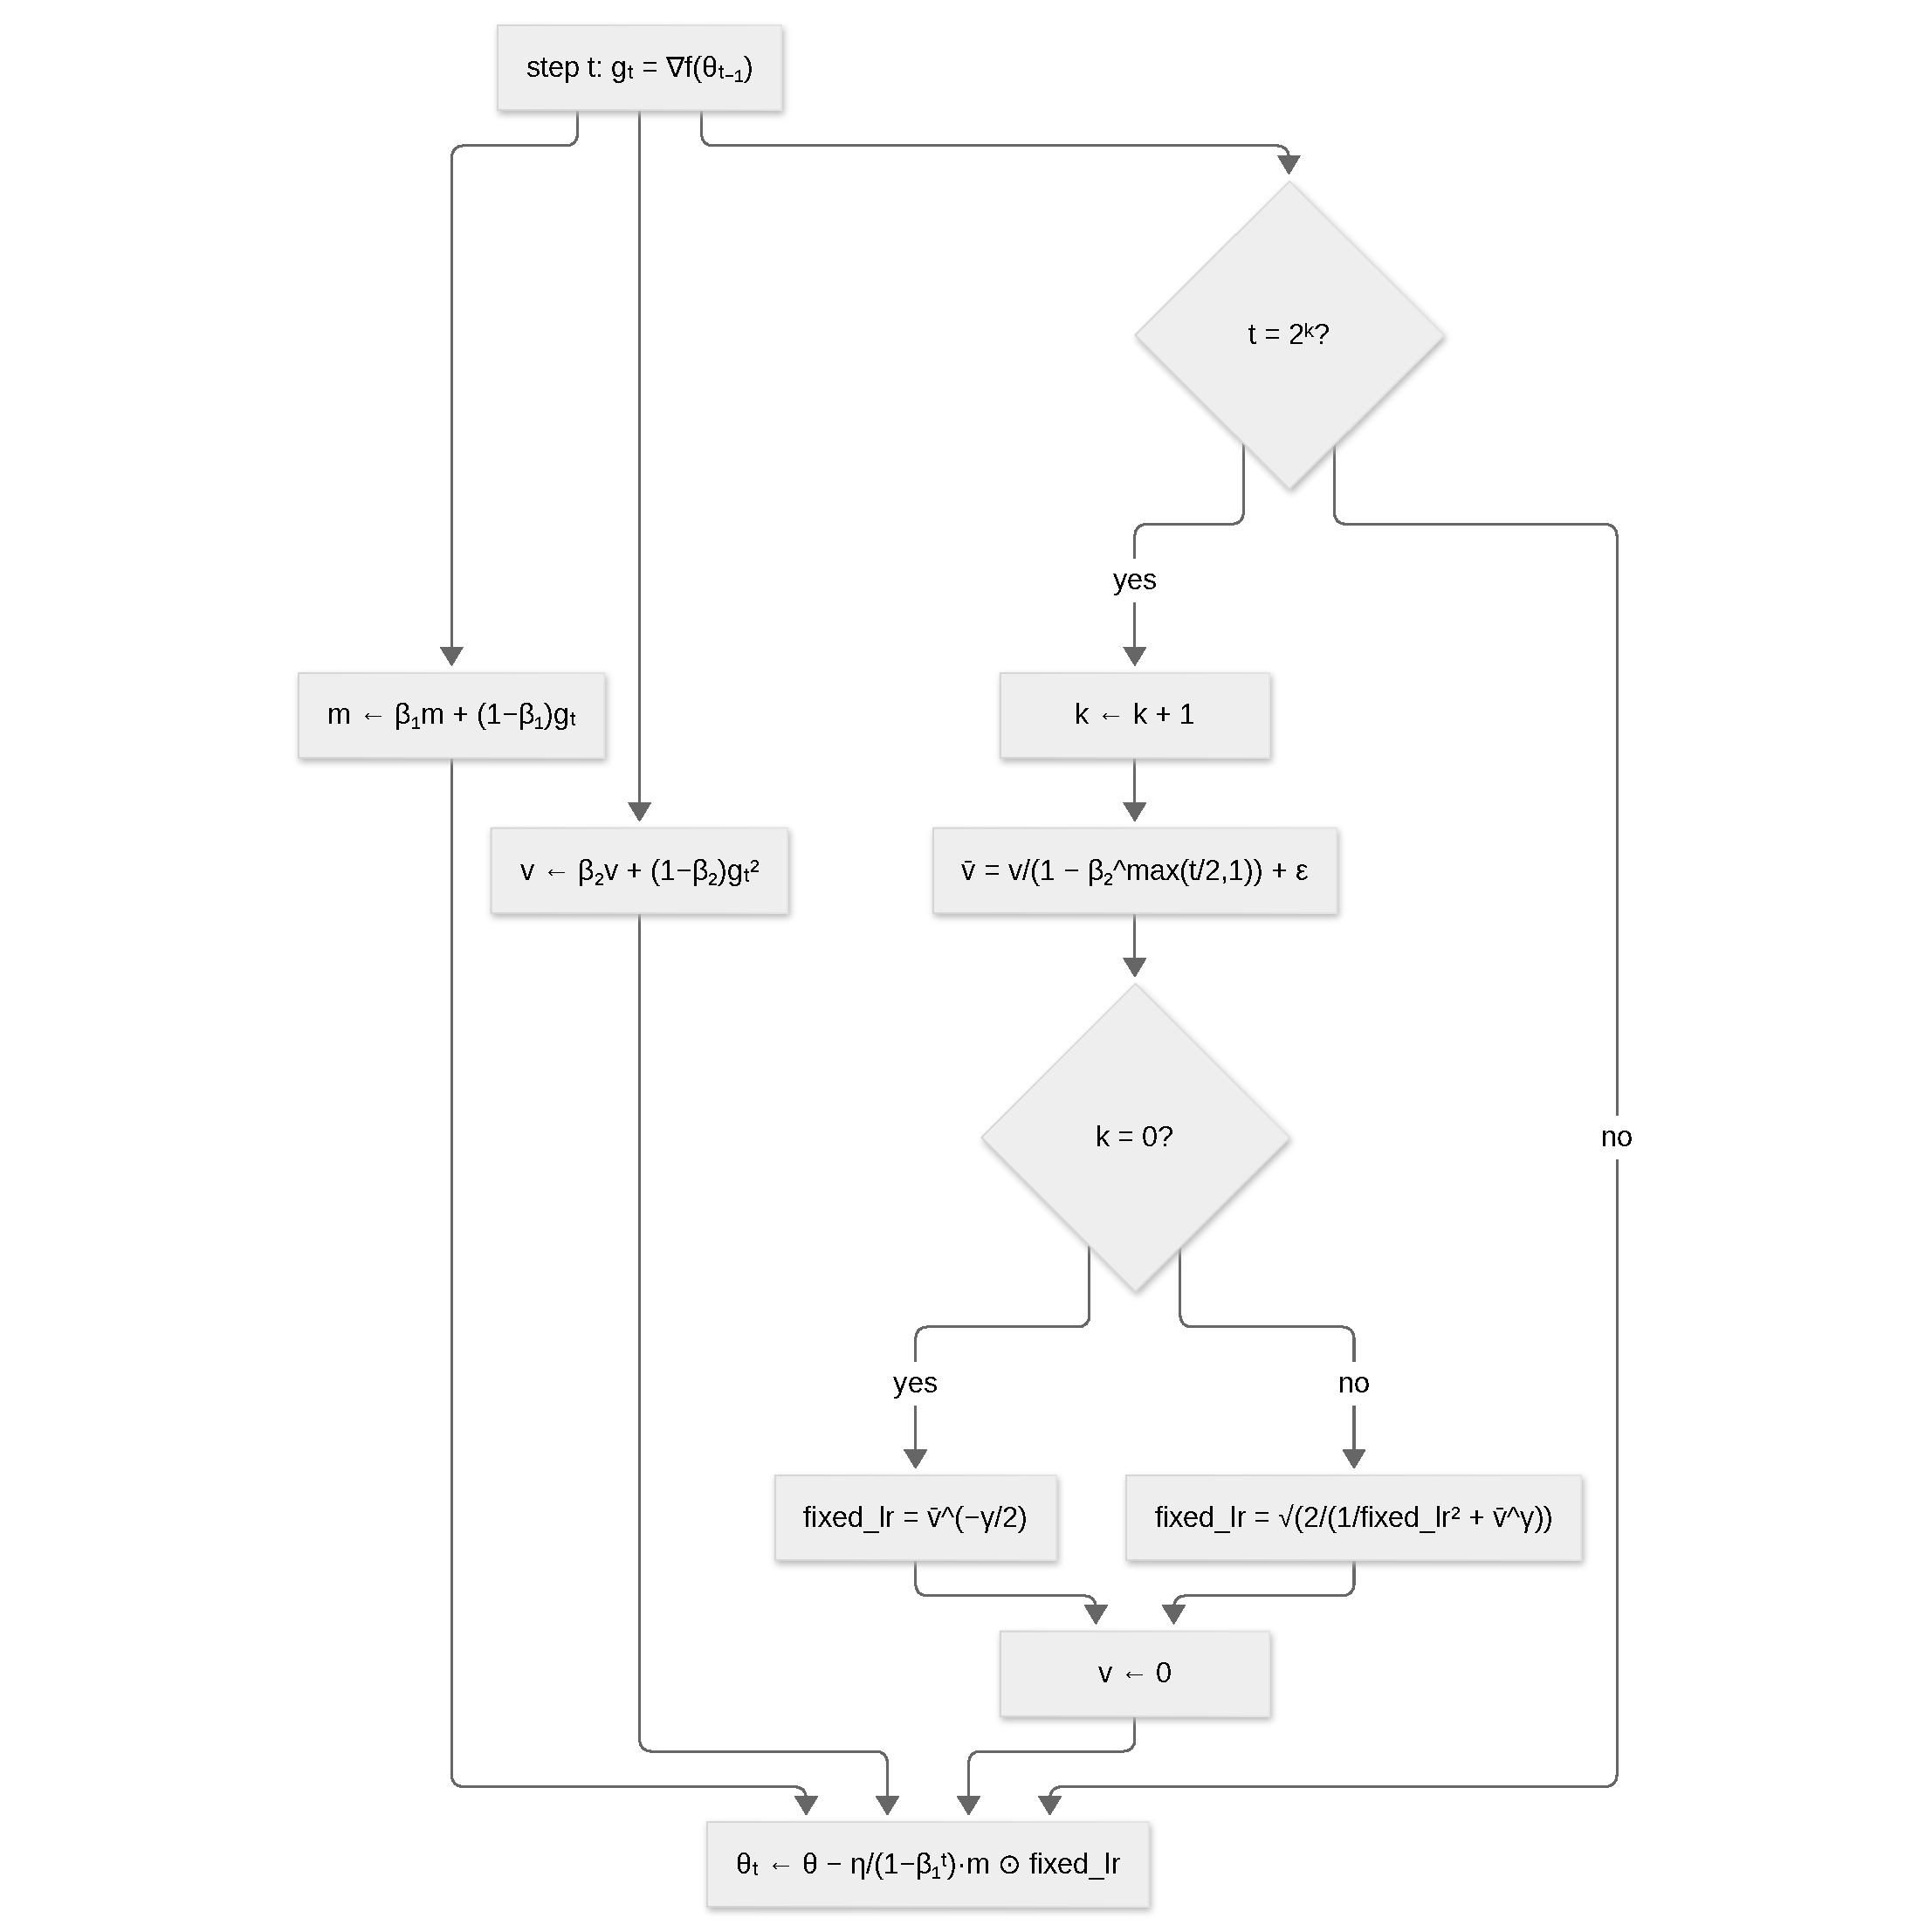
\includegraphics{../paper/figures/optimizers/anon.pdf}}
\caption{Flujo por paso de Anon: el precondicionador IDU refrescado en potencias de dos, con adaptividad ajustable $\gamma$ y una actualización de momentum con corrección de sesgo.}
\label{fig:opt-anon}
\end{figure}
Anon \citep{anon2026anon} introduce adaptividad ajustable continuamente mediante un único parámetro $\gamma \in \mathbb{R}$, cerrando la brecha entre comportamientos tipo SGD ($\gamma=0$) y tipo Adam ($\gamma=1$), y extrapolando más allá de ambos. La innovación central es el mecanismo Incremental Delay Update (IDU), que permite convergencia estable a través de todo el espectro de adaptividad de valores reales:

\begin{align}
m_t &= \beta_1 m_{t-1} + (1-\beta_1) g_t \quad\text{(momento de primer orden)}\\
v_t &= \beta_2 v_{t-1} + (1-\beta_2) g_t^2 \quad\text{(momento de segundo orden)}\\
\bar{v}_t &= \frac{v_t}{1-\beta_2^{\max(t,1)}} + \epsilon \quad\text{(momento de segundo orden con corrección de sesgo)}\\
\text{fixed\_lr}_k &= \begin{cases}
\bar{v}_k^{-\gamma/2} & \text{si } k = 0 \\
\sqrt{2 / \left(\frac{1}{\text{fixed\_lr}_{k-1}^2} + \bar{v}_k^\gamma\right)} & \text{si } k > 0
\end{cases}\\
\theta_{t+1} &= \theta_t - \frac{\eta}{1-\beta_1^t} \cdot m_t \odot \text{fixed\_lr}_{\lfloor\log_2 t\rfloor}
\end{align}

A diferencia de los optimizadores adaptativos estándar, IDU actualiza el precondicionador solo en potencias de dos ($t = 2^k$), acumulando estadísticas de gradiente entre actualizaciones y agregándolas recursivamente. Este acumulador suave y multiescala evita el seguimiento estricto del máximo de AMSGrad mientras estabiliza demostrablemente la convergencia para cualquier $\gamma \in \mathbb{R}$. El parámetro $\gamma$ controla directamente la adaptividad: $\gamma > 1$ acelera la salida de puntos de silla (favorable para arquitecturas complejas), $\gamma = 1$ recupera el comportamiento tipo Adam, $\gamma = 0$ produce escalado tipo SGD, y $\gamma < 0$ se sesga hacia mínimos más planos (beneficioso para arquitecturas clásicas como CNNs).

\begin{algorithm}[H]
\caption{Anon (Adaptivity Non-restricted Optimizer con IDU)}
\label{alg:anon}
\begin{algorithmic}[1]
\Require Parámetros iniciales $\theta_0$, tasa de aprendizaje $\eta$, $\beta_1, \beta_2$, tolerancia $\epsilon$, adaptividad $\gamma \in \mathbb{R}$
\Ensure Parámetros actualizados $\theta_T$
\State Inicializar: $m \gets 0$, $v \gets 0$, $fixed\_lr \gets 0$, paso $t \gets 0$, contador IDU $k \gets -1$
\For{$t = 1, 2, \ldots, T$}
    \State $g_t \gets \nabla f(\theta_{t-1})$
    \State $m \gets \beta_1 m + (1-\beta_1) g_t$
    \State $v \gets \beta_2 v + (1-\beta_2) g_t^2$
    \If{$t = 2^k$}
        \State $k \gets k+1$
        \State $\bar{v} \gets v/(1 - \beta_2^{\max(t/2,1)}) + \epsilon$
        \If{$k = 0$}
            \State fixed\_lr $\gets \bar{v}^{-\gamma/2}$
        \Else
            \State fixed\_lr $\gets \sqrt{2 / (1/\text{fixed\_lr}^2 + \bar{v}^\gamma)}$
        \EndIf
        \State $v \gets 0$
    \EndIf
    \State $\theta_t \gets \theta_{t-1} - \frac{\eta}{1-\beta_1^t} \cdot m \odot \text{fixed\_lr}$
\EndFor
\Return $\theta_T$
\end{algorithmic}
\end{algorithm}

\paragraph{Contras.}
\begin{itemize}[leftmargin=*]
\item Mantiene tres búferes de estado ($m$, $v$, fixed\_lr) y refresca el precondicionador con una programación logarítmica.
\item El parámetro de adaptividad $\gamma$ debe seleccionarse por arquitectura.
\end{itemize}

\paragraph{Ventajas.}
\begin{itemize}[leftmargin=*]
\item Misma clase de complejidad $\mathcal{O}(n)$ por paso que AdamW, con adaptividad ajustable de forma continua.
\item IDU alcanza demostrablemente regret $\mathcal{O}(\sqrt{T})$ para problemas convexos y $\mathcal{O}(\ln T/\sqrt{T})$ para entornos no convexos.
\end{itemize}

\paragraph{Prodigy (Approximating the Distance Estimate).}
\begin{figure}[H]
\centering
\fitfigure{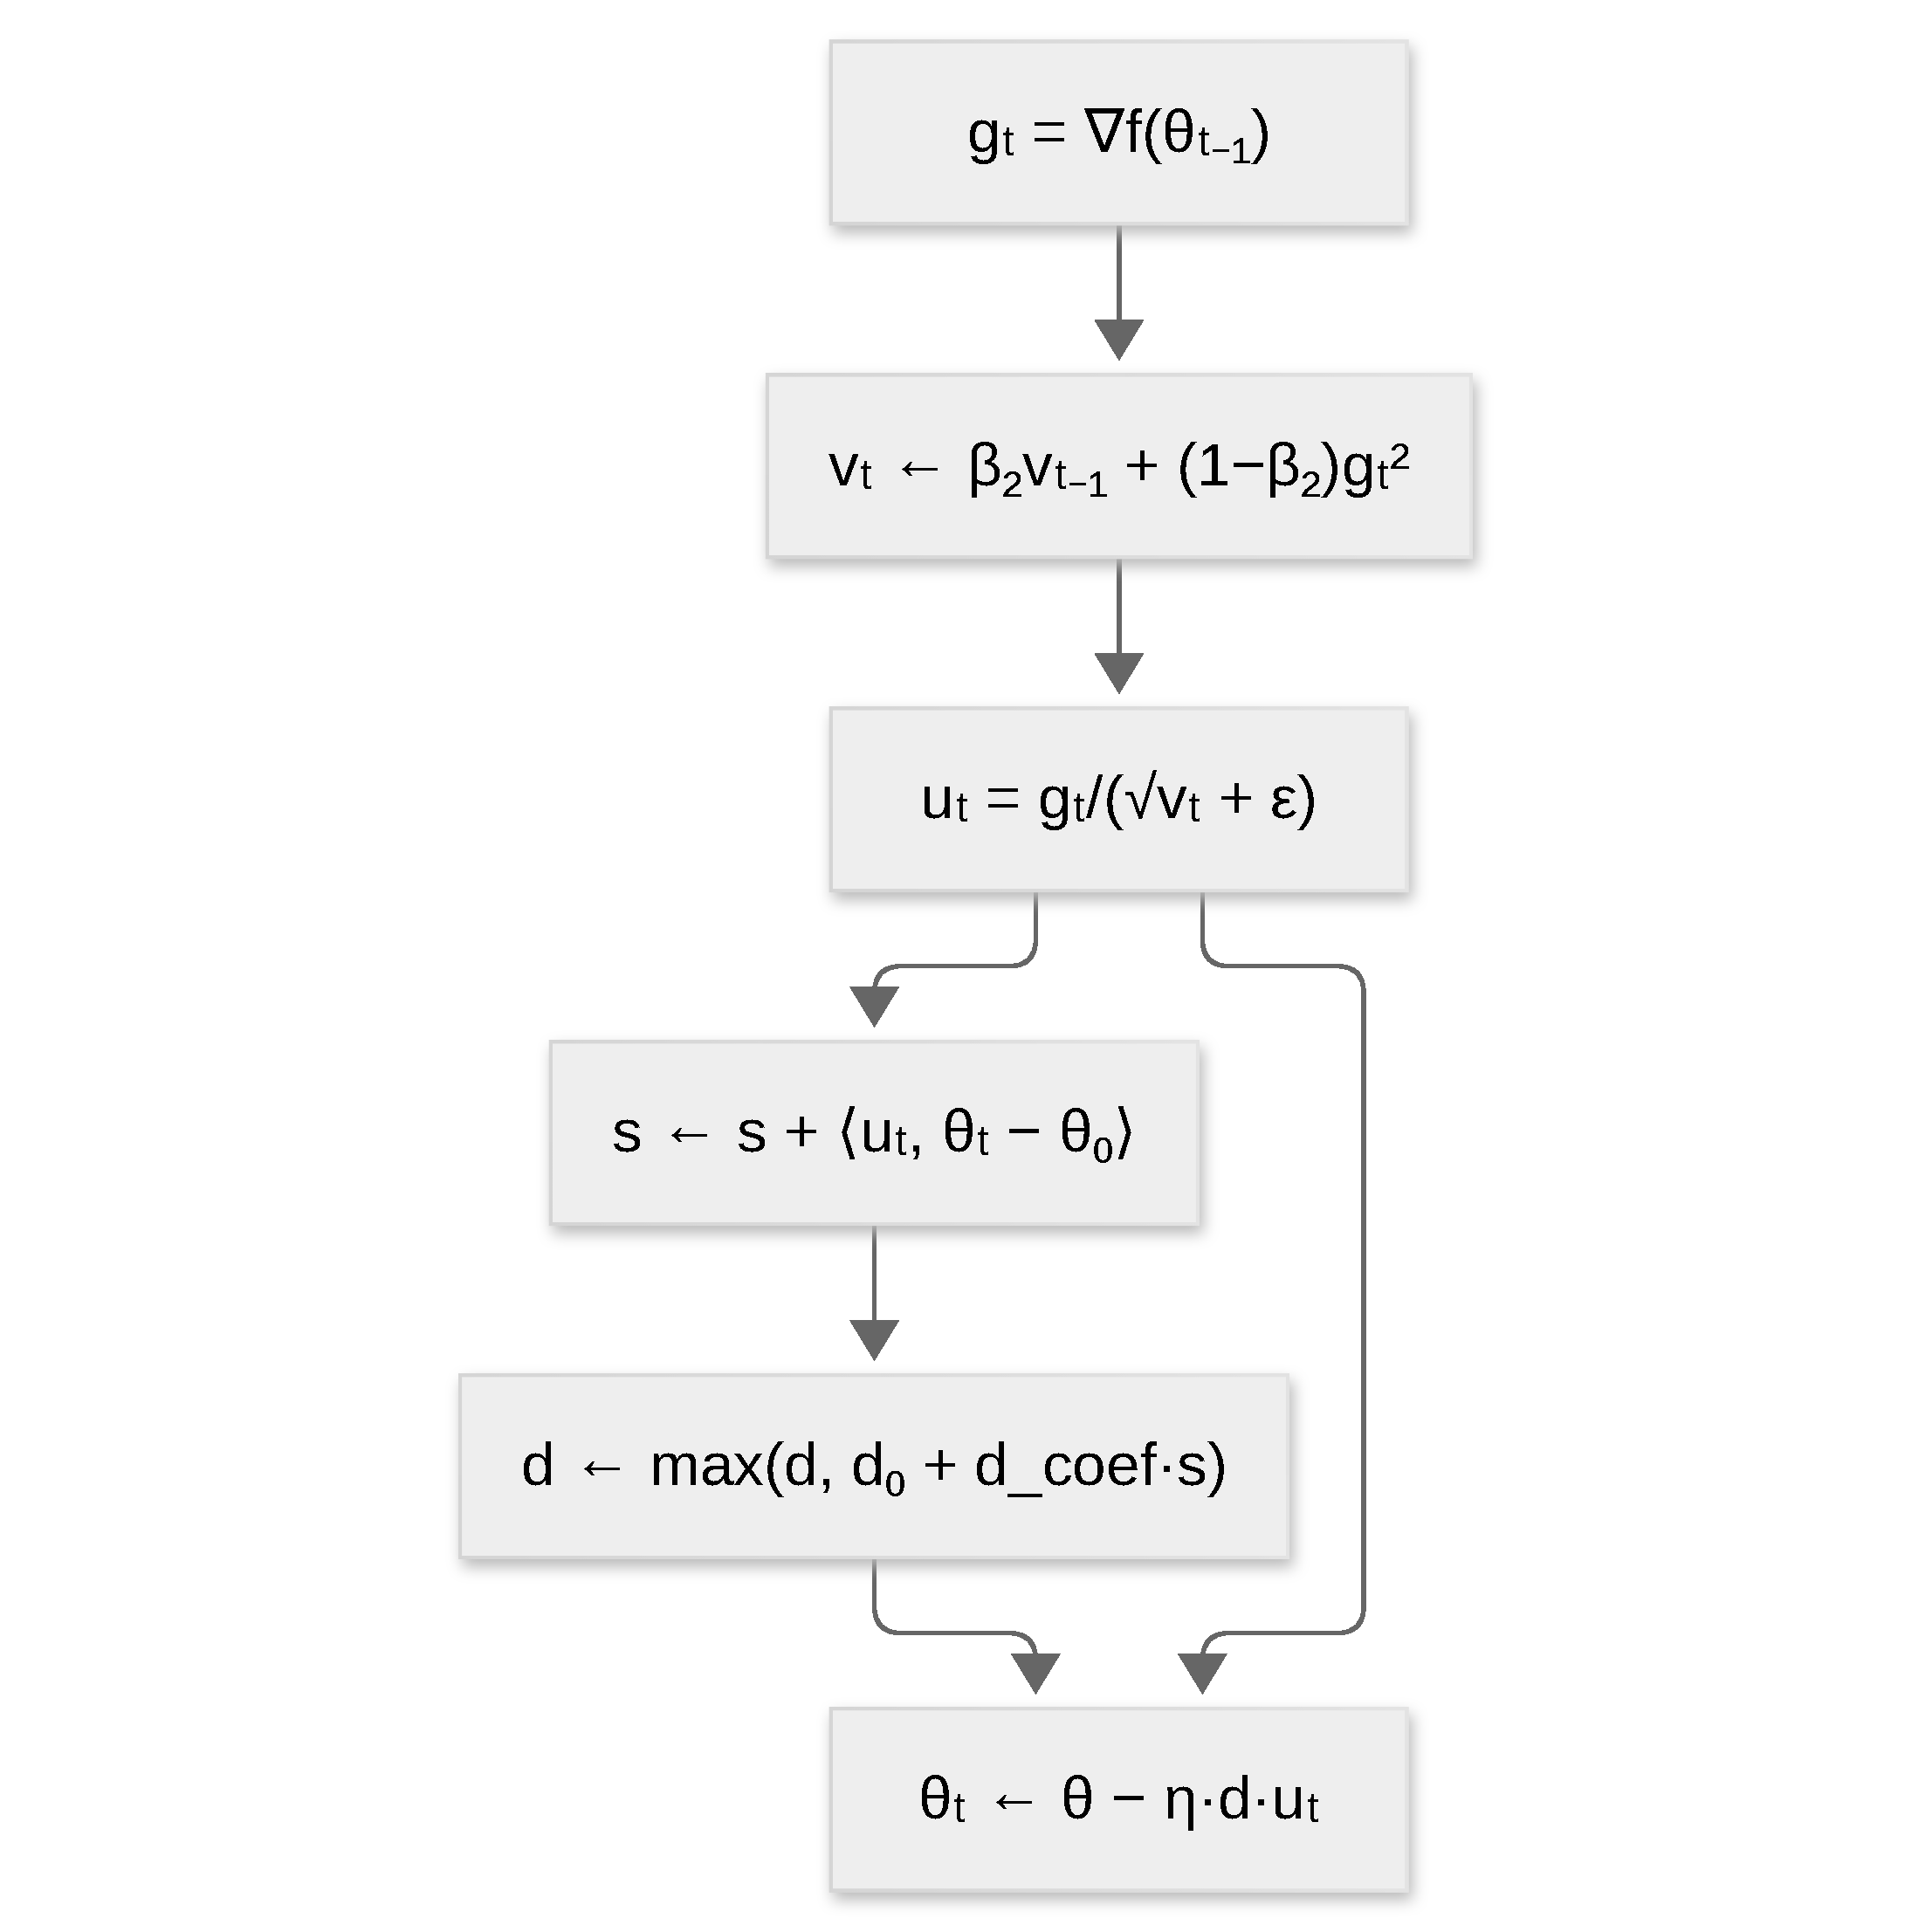
\includegraphics{../paper/figures/optimizers/prodigy.pdf}}
\caption{Flujo por paso de Prodigy: una estimación de distancia signada acumulativa que escala el paso adaptativo sin programación de tasa de aprendizaje.}
\label{fig:opt-prodigy}
\end{figure}
Prodigy adapta la escala efectiva del paso mediante una estadística tipo distancia acumulativa, eliminando la necesidad de ajuste explícito de la tasa de aprendizaje. El algoritmo mantiene una estimación de distancia acumulativa:
\begin{align}
u_t &= \frac{g_t}{\sqrt{v_t}+\epsilon} \quad\text{(paso adaptativo no normalizado)} \\
s_t &= s_{t-1} + \langle u_t, \theta_t - \theta_0 \rangle \quad\text{(distancia signada acumulativa)} \\
d_t &= \max(d_{t-1}, d_0 + d_{\text{coef}} \cdot s_t) \quad\text{(estimación de distancia con cota inferior)} \\
\theta_{t+1} &= \theta_t - \eta \cdot d_t \cdot u_t
\end{align}
donde $d_0$ es una cota inicial y $d_{\text{coef}}$ controla qué tan agresivamente se adapta la estimación. La estimación de distancia $d_t$ captura la magnitud combinada de gradientes pasados ponderada por el desplazamiento real de los parámetros, implementando una tasa de aprendizaje efectiva implícita.

\begin{algorithm}[H]
\caption{Prodigy (Approximating the Distance Estimate)}
\label{alg:prodigy}
\begin{algorithmic}[1]
\Require Parámetros iniciales $\theta_0$, tasa de aprendizaje $\eta$, coeficiente $d_{\text{coef}}$, distancia inicial $d_0 > 0$
\Ensure Parámetros actualizados $\theta_T$
\State Inicializar: $s \gets 0$ (distancia signada acumulativa), $d \gets d_0$
\For{$t = 1, 2, \ldots, T$}
    \State $g_t \gets \nabla f(\theta_{t-1})$
    \State $v_t \gets \beta_2 v_{t-1} + (1-\beta_2) g_t^2$ \Comment{Segundo momento}
    \State $u_t \gets g_t / (\sqrt{v_t} + \epsilon)$ \Comment{Adaptativo no normalizado}
    \State Actualizar distancia: $s \gets s + \langle u_t, \theta_t - \theta_0 \rangle$ \Comment{Distancia signada}
    \State $d \gets \max(d, d_0 + d_{\text{coef}} \cdot s)$ \Comment{Distancia con cota inferior}
    \State $\theta_t \gets \theta_{t-1} - \eta \cdot d \cdot u_t$ \Comment{Actualización escalada por distancia}
\EndFor
\Return $\theta_T$
\end{algorithmic}
\end{algorithm}

\paragraph{Contras.}
\begin{itemize}[leftmargin=*]
\item Introduce los hiperparámetros $d_0$ y $d_{\text{coef}}$ para la estimación de distancia.
\item Añade un paso de contabilidad de producto interno por iteración.
\end{itemize}

\paragraph{Ventajas.}
\begin{itemize}[leftmargin=*]
\item Elimina el ajuste y la programación explícitos de la tasa de aprendizaje.
\item Convergencia robusta en distintas escalas de problemas y tamaños de lote.
\end{itemize}

\subsection{Optimizadores de Segundo Orden, Geométricos y de Ortogonalidad}
\paragraph{Shampoo (Precondicionamiento Matricial mediante Productos de Kronecker).}
\begin{figure}[H]
\centering
\fitfigure{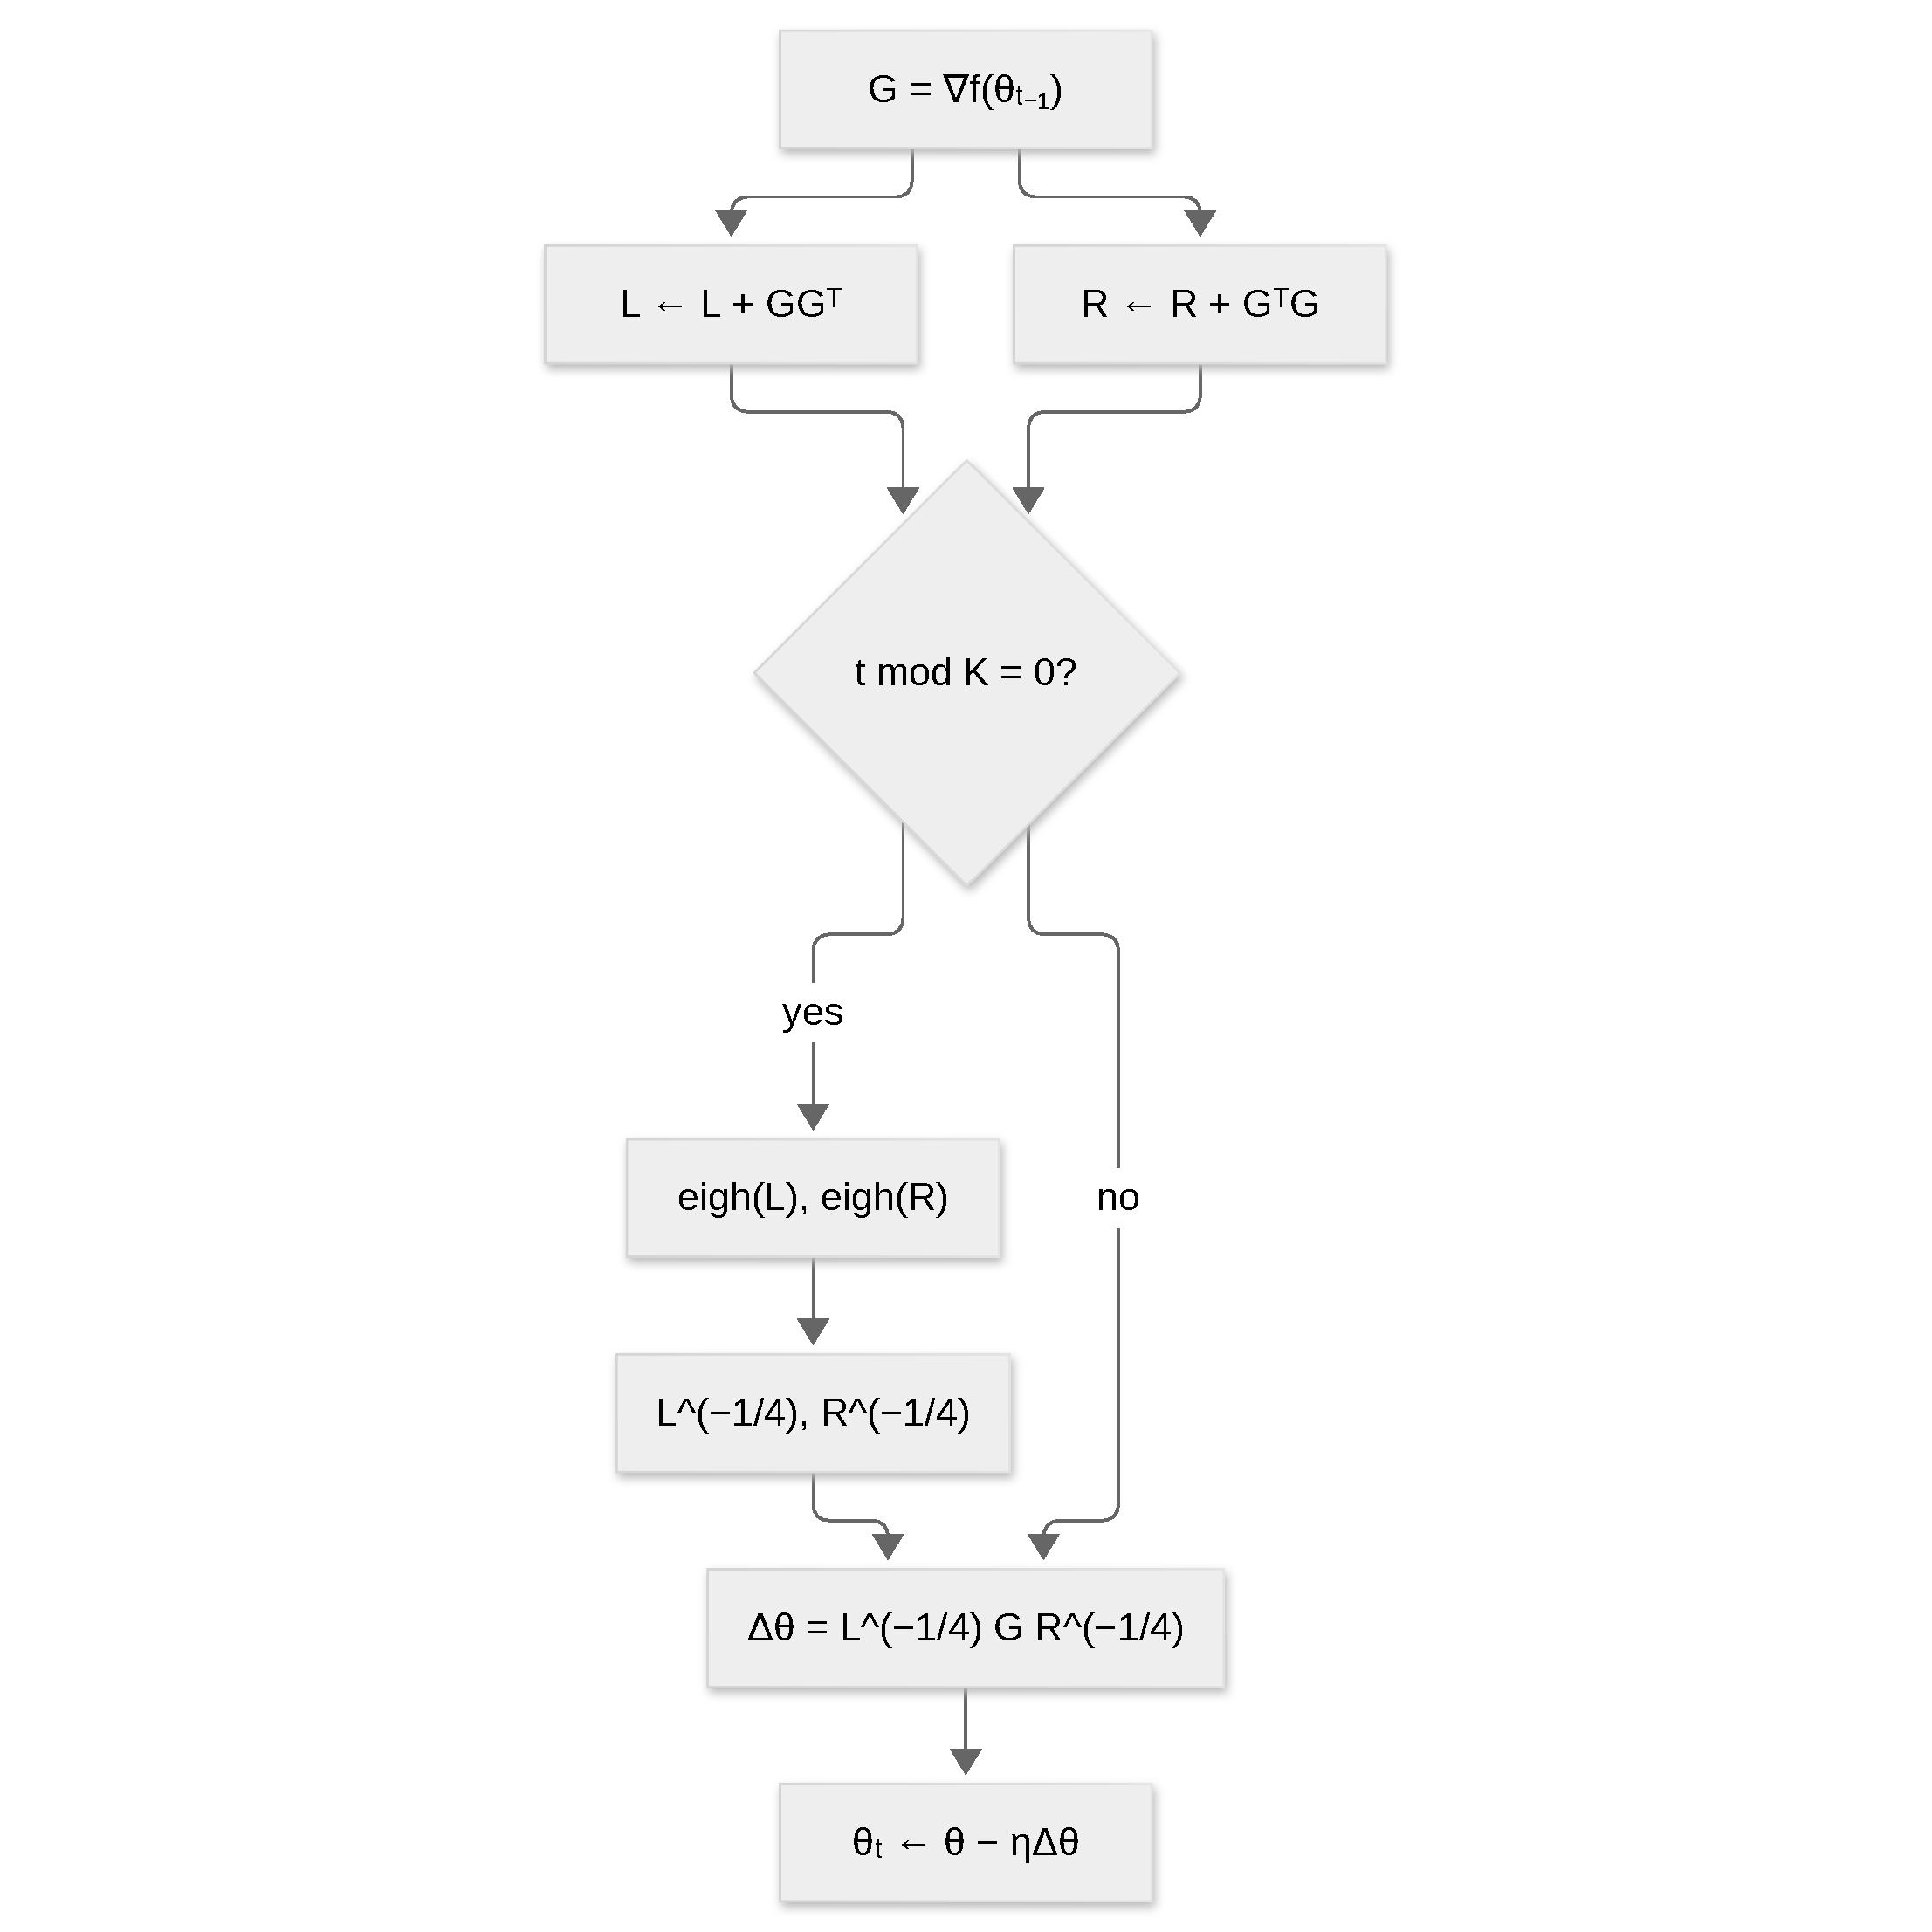
\includegraphics{../paper/figures/optimizers/shampoo.pdf}}
\caption{Flujo por paso de Shampoo: matrices de Gram factorizadas por Kronecker, eigendescomposición periódica y precondicionamiento del gradiente con raíz cuarta.}
\label{fig:opt-shampoo}
\end{figure}
Shampoo es un \textbf{método estructurado de segundo orden} que calcula precondicionadores matriciales a partir de estadísticas de producto exterior con estructura de Kronecker. Para una matriz de parámetros 2D $W \in \mathbb{R}^{m \times n}$:
\begin{align}
L_t &= L_{t-1} + G_t G_t^\top \quad\text{(matriz de Gram izquierda/filas, $m \times m$)} \\
R_t &= R_{t-1} + G_t^\top G_t \quad\text{(matriz de Gram derecha/columnas, $n \times n$)} \\
L_t^{-1/4} &= Q_L (\Lambda_L)^{-1/4} Q_L^\top \quad\text{(mediante eigendescomposición)} \\
R_t^{-1/4} &= Q_R (\Lambda_R)^{-1/4} Q_R^\top \\
\Delta W_t &= L_t^{-1/4} G_t R_t^{-1/4} \quad\text{(gradiente precondicionado)}
\end{align}
Shampoo aproxima el precondicionador de matriz completa de Adagrad $H^{-1/2}$ (donde $H$ es el Hessiano) utilizando estructura factorizada de Kronecker. En lugar de almacenar un precondicionador de $(mn) \times (mn)$, Shampoo mantiene dos matrices más pequeñas ($m \times m$ y $n \times n$), capturando correlaciones entre parámetros dentro y entre grupos. Las eigendescomposiciones se realizan periódicamente (e.g., cada $K=10$ pasos) para amortizar el costo.

\begin{algorithm}[H]
\caption{Shampoo (Precondicionamiento Matricial mediante Productos de Kronecker)}
\label{alg:shampoo}
\begin{algorithmic}[1]
\Require Parámetros iniciales $\theta_0$, tasa de aprendizaje $\eta$, intervalo de eigendescomposición $K$
\Ensure Parámetros actualizados $\theta_T$
\State Inicializar: $L \gets \epsilon I_m$, $R \gets \epsilon I_n$ (matrices de Gram izquierda y derecha)
\For{$t = 1, 2, \ldots, T$}
    \State $G \gets \nabla f(\theta_{t-1})$ \Comment{Gradiente}
    \State Actualizar matrices de Gram: $L \gets L + G G^\top$, $R \gets R + G^\top G$
    \If{$t \mod K == 0$}
        \State $Q_L, \Lambda_L \gets \text{eigh}(L)$ \Comment{Eigendescomposición de $L$}
        \State $Q_R, \Lambda_R \gets \text{eigh}(R)$ \Comment{Eigendescomposición de $R$}
        \State $L^{-1/4} \gets Q_L (\Lambda_L + \epsilon)^{-1/4} Q_L^\top$
        \State $R^{-1/4} \gets Q_R (\Lambda_R + \epsilon)^{-1/4} Q_R^\top$
    \EndIf
    \State $\Delta \theta \gets L^{-1/4} G R^{-1/4}$ \Comment{Gradiente precondicionado}
    \State $\theta_t \gets \theta_{t-1} - \eta \cdot \Delta \theta$
\EndFor
\Return $\theta_T$
\end{algorithmic}
\end{algorithm}

\paragraph{Contras.}
\begin{itemize}[leftmargin=*]
\item Eigendescomposiciones periódicas $O(m^3+n^3)$ y mayor cómputo por paso.
\item Asume estructura de parámetros 2D; los embeddings y sesgos requieren manejo aparte.
\end{itemize}

\paragraph{Ventajas.}
\begin{itemize}[leftmargin=*]
\item Precondicionamiento de segundo orden factorizado por Kronecker sin una matriz densa $(mn)\times(mn)$.
\item Demostrado efectivo a escala de producción y adecuado para matrices transformer de alto rango, con mejor condicionamiento y convergencia acelerada.
\end{itemize}

\paragraph{SOAP (Shampoo with Adam in eigenbasis).}
\begin{figure}[H]
\centering
\fitfigure{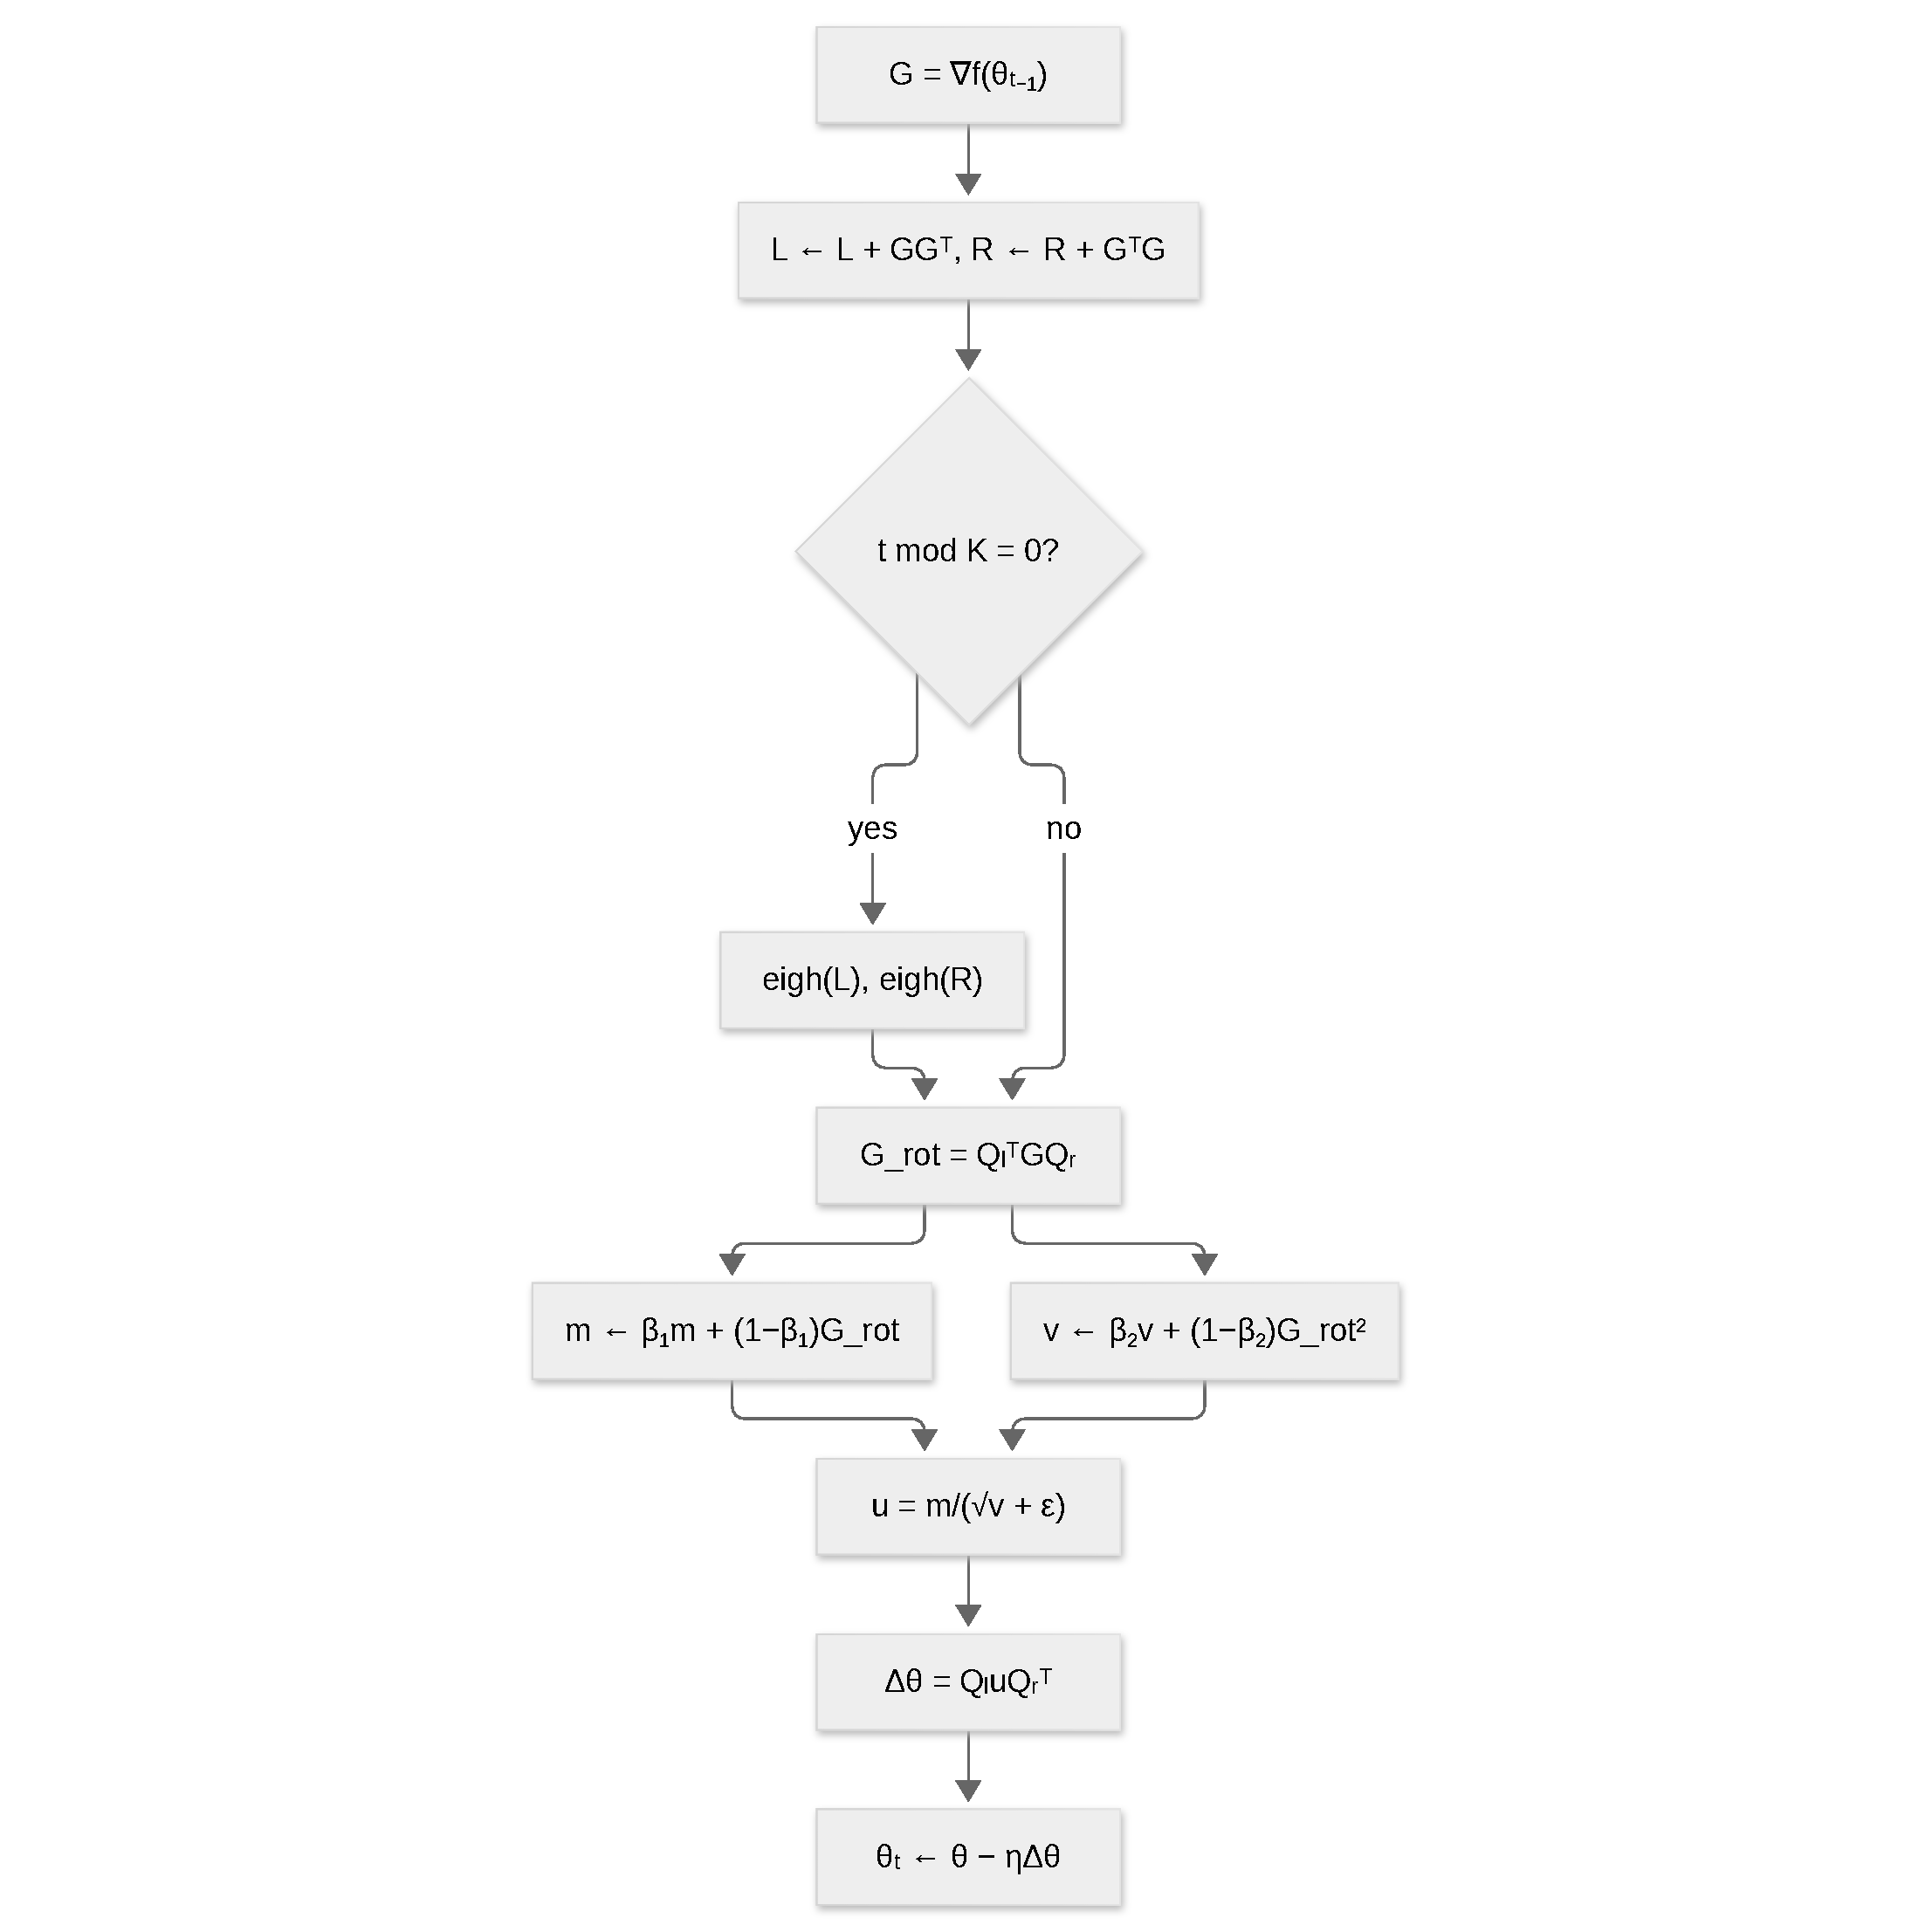
\includegraphics{../paper/figures/optimizers/soap.pdf}}
\caption{Flujo por paso de SOAP: momentos de Adam en la base de eigenvectores de Shampoo, rotados de vuelta al espacio de parámetros.}
\label{fig:opt-soap}
\end{figure}
SOAP es una variante simplificada de Shampoo que desacopla el precondicionamiento del seguimiento de momento. En lugar de álgebra matricial compleja sobre gradientes precondicionados, SOAP ejecuta Adam estándar en la base de eigenvectores de los precondicionadores de Shampoo:
\begin{align}
L_t &= L_{t-1} + G_t G_t^\top, \quad R_t = R_{t-1} + G_t^\top G_t \quad\text{(acumulación de Gram)} \\
Q_L, \Lambda_L &= \text{eigh}(L_t), \quad Q_R, \Lambda_R = \text{eigh}(R_t) \quad\text{(eigendescomposición periódica)} \\
G_t^{\text{rot}} &= Q_L^\top G_t Q_R \quad\text{(rotar gradiente a la base de eigenvectores)} \\
m_t^{\text{rot}} &= \beta_1 m_{t-1}^{\text{rot}} + (1-\beta_1) G_t^{\text{rot}} \\
v_t^{\text{rot}} &= \beta_2 v_{t-1}^{\text{rot}} + (1-\beta_2)(G_t^{\text{rot}})^2 \quad\text{(Adam en el espacio rotado)} \\
U_t^{\text{rot}} &= \frac{m_t^{\text{rot}}}{\sqrt{v_t^{\text{rot}}}+\epsilon}, \quad U_t = Q_L U_t^{\text{rot}} Q_R^\top \quad\text{(rotar de vuelta)}
\end{align}
La idea clave: todo el seguimiento de momento ocurre en la base de eigenvectores bien condicionada, simplificando la estabilidad numérica y el análisis teórico.

\begin{algorithm}[H]
\caption{SOAP (Shampoo with Adam in Eigenbasis)}
\label{alg:soap}
\begin{algorithmic}[1]
\Require Parámetros iniciales $\theta_0$, tasa de aprendizaje $\eta$, $\beta_1, \beta_2$, intervalo de eigendescomposición $K$
\Ensure Parámetros actualizados $\theta_T$
\State Inicializar: $L \gets \epsilon I_m$, $R \gets \epsilon I_n$, $m \gets 0$, $v \gets 0$
\For{$t = 1, 2, \ldots, T$}
    \State $G \gets \nabla f(\theta_{t-1})$ \Comment{Gradiente}
    \State Actualizar Gram: $L \gets L + G G^\top$, $R \gets R + G^\top G$
    \If{$t \mod K == 0$}
        \State $Q_L, \Lambda_L \gets \text{eigh}(L)$, $Q_R, \Lambda_R \gets \text{eigh}(R)$
    \EndIf
    \State $G^{\text{rot}} \gets Q_L^\top G Q_R$ \Comment{Rotar gradiente a la base de eigenvectores}
    \State $m \gets \beta_1 m + (1-\beta_1) G^{\text{rot}}$ \Comment{Media móvil exponencial (corregir sesgo externamente)}
    \State $v \gets \beta_2 v + (1-\beta_2) (G^{\text{rot}})^2$ \Comment{Segundo momento (corregir sesgo externamente)}
    \State $u \gets m / (\sqrt{v} + \epsilon)$ \Comment{Paso adaptativo en la base de eigenvectores}
    \State $\Delta \theta \gets Q_L u Q_R^\top$ \Comment{Rotar de vuelta al espacio de parámetros}
    \State $\theta_t \gets \theta_{t-1} - \eta \cdot \Delta \theta$
\EndFor
\Return $\theta_T$
\end{algorithmic}
\end{algorithm}

\paragraph{Contras.}
\begin{itemize}[leftmargin=*]
\item Hereda el costo de eigendescomposición periódica de Shampoo.
\item La rotación y la rotación inversa añaden multiplicaciones de matrices por paso.
\end{itemize}

\paragraph{Ventajas.}
\begin{itemize}[leftmargin=*]
\item Combina la estructura de curvatura explícita de Shampoo con la mecánica de momentum probada de Adam.
\item A menudo más limpio y estable que Shampoo completo, con eigendescomposiciones amortizadas cada $K$ pasos.
\end{itemize}

\paragraph{Lion (EvoLved Sign Momentum).}
\begin{figure}[H]
\centering
\fitfigure{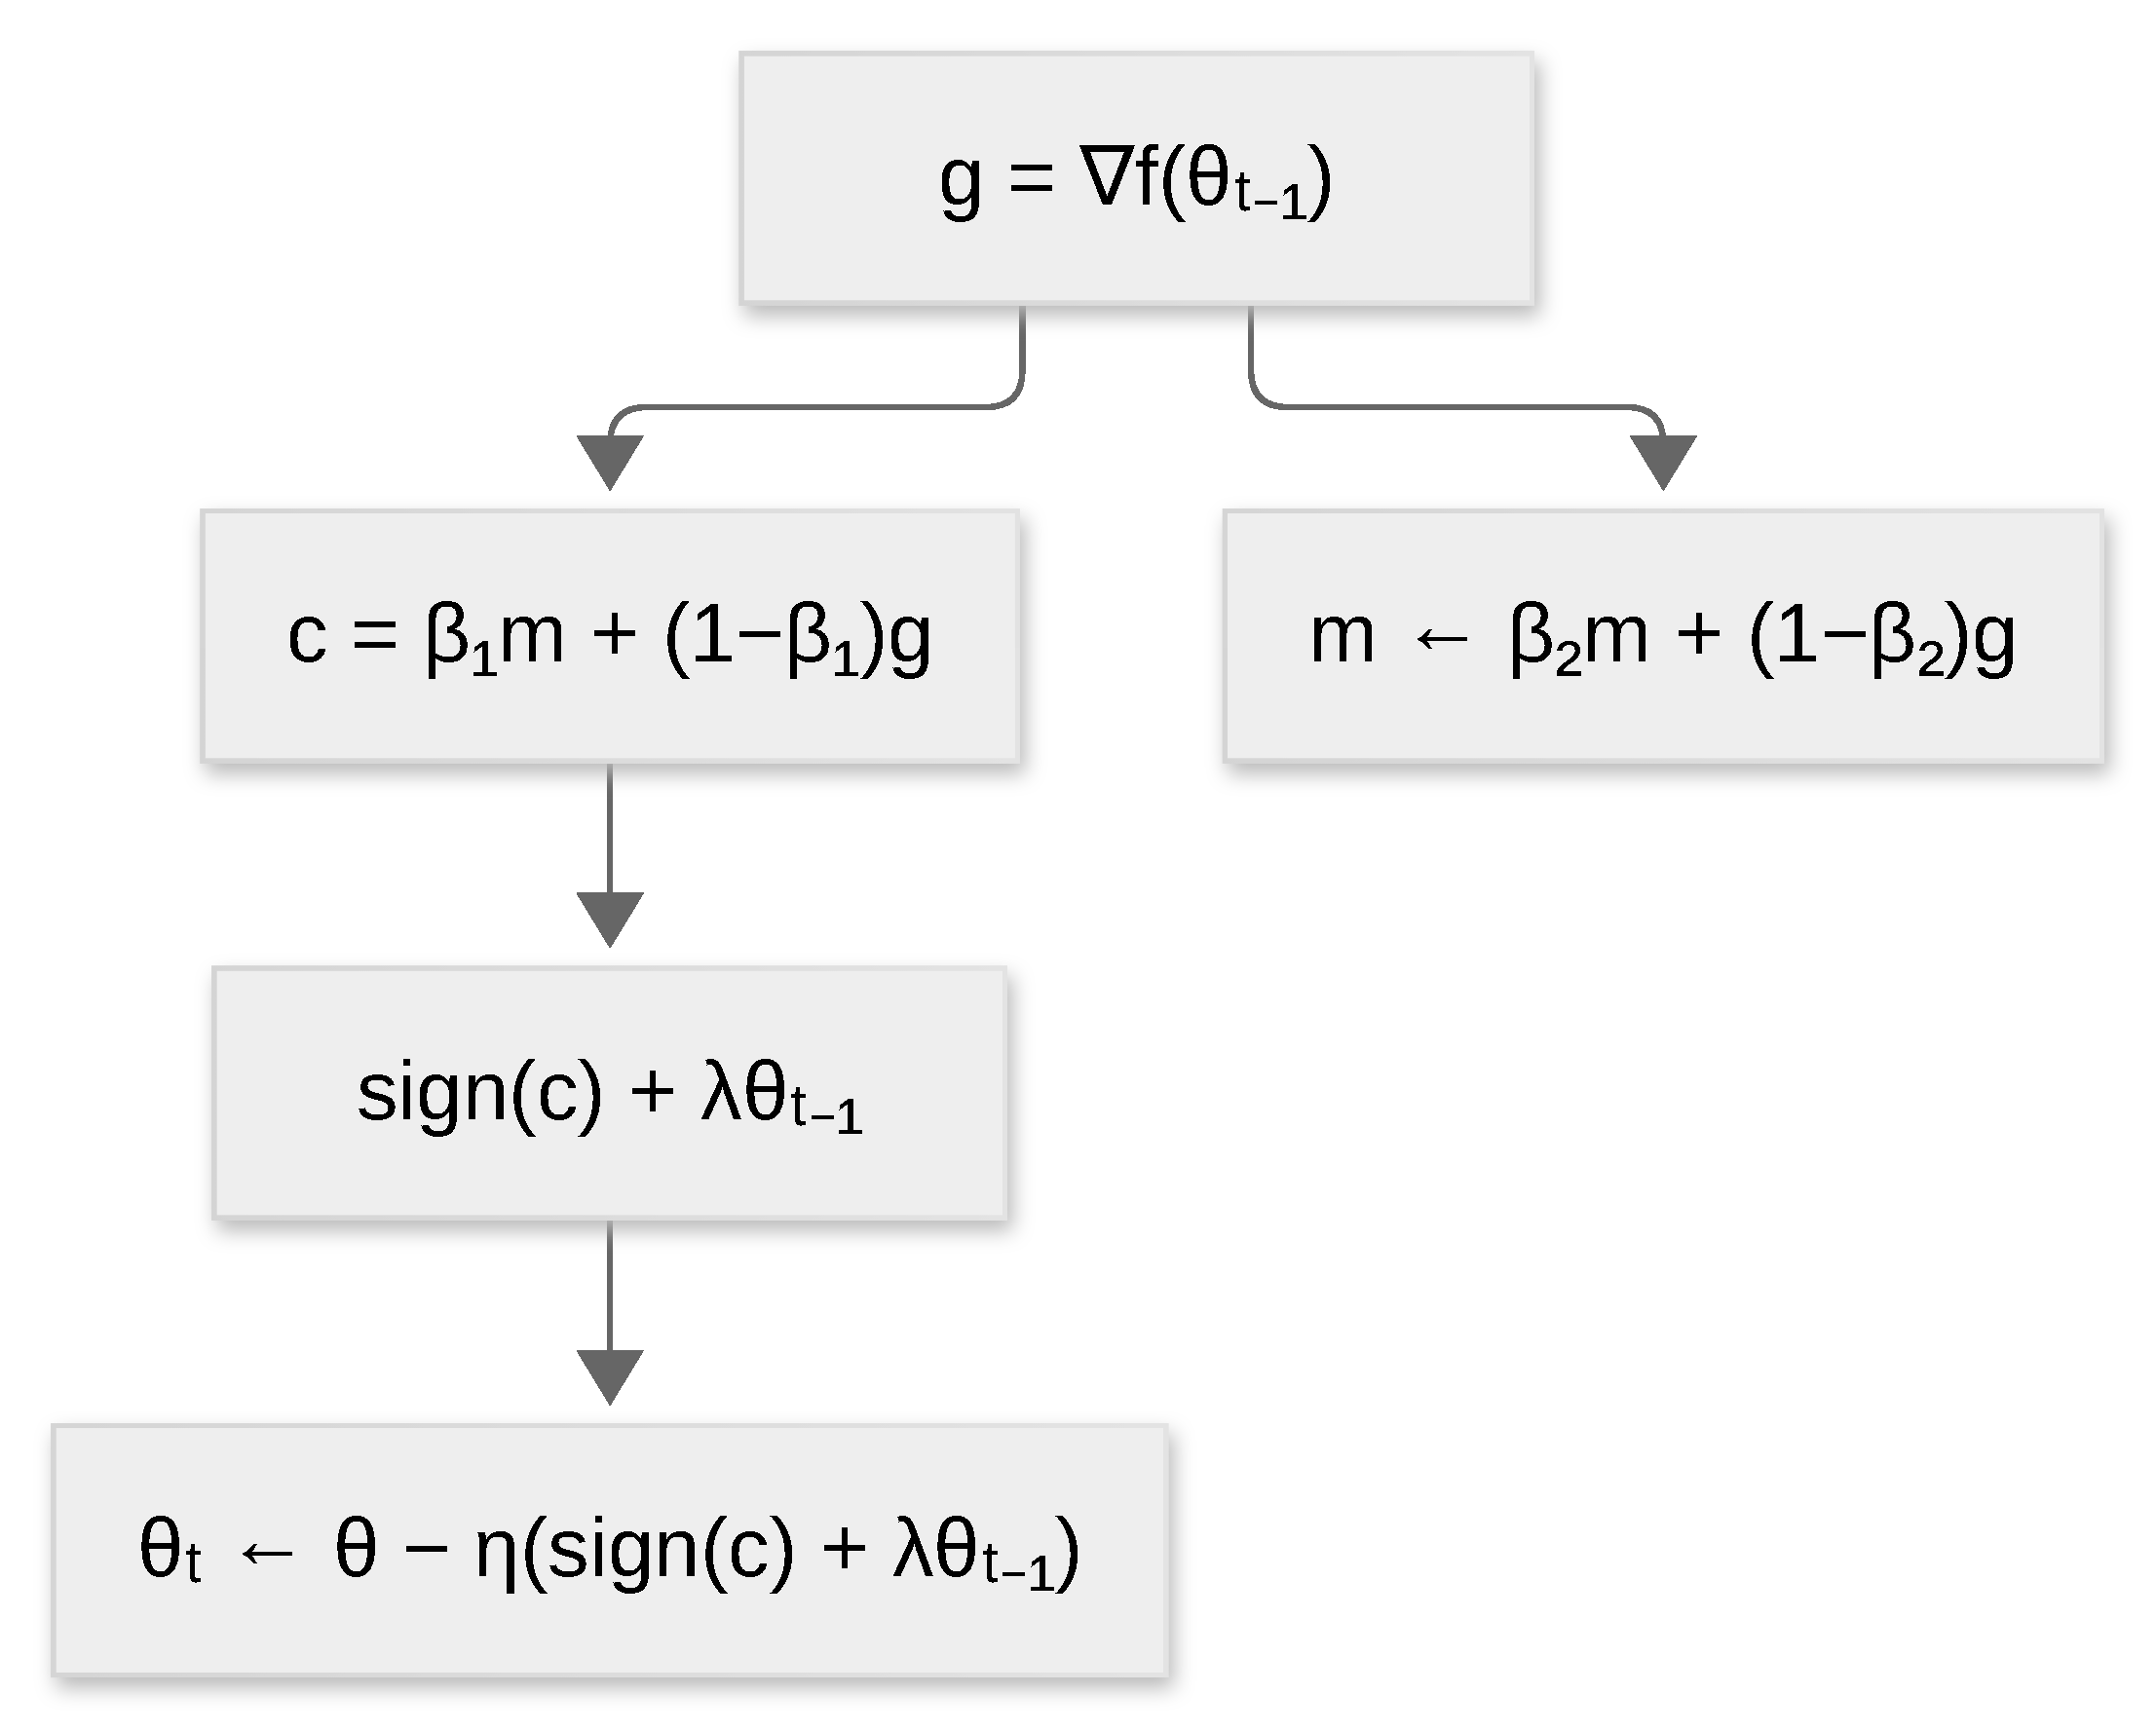
\includegraphics{../paper/figures/optimizers/lion.pdf}}
\caption{Flujo por paso de Lion: actualización por signo del momentum con acumulación de momentum desacoplada y decaimiento de pesos.}
\label{fig:opt-lion}
\end{figure}
Lion logra una \textbf{sobrecarga de memoria mínima} al usar actualizaciones basadas en signo en lugar de escalado adaptativo completo:
\begin{align}
c_t &= \beta_1 m_t + (1-\beta_1) g_t \quad\text{(entrada de momento)} \\
\theta_{t+1} &= \theta_t - \eta \left(\text{sign}(c_t) + \lambda\theta_t\right) \quad\text{(actualización con operador signo)} \\
m_{t+1} &= \beta_2 m_t + (1-\beta_2) g_t \quad\text{(acumulación de momento)}
\end{align}
Todas las operaciones de escalado elemento a elemento se reemplazan con \texttt{sign()}, que produce $\{-1, 0, +1\}$. Esto reduce drásticamente la memoria en comparación con métodos tipo Adam: Lion almacena solo el búfer de momento, sin varianza de segundo momento.

\begin{algorithm}[H]
\caption{Lion (EvoLved Sign Momentum)}
\label{alg:lion}
\begin{algorithmic}[1]
\Require Parámetros iniciales $\theta_0$, tasa de aprendizaje $\eta$, $\beta_1, \beta_2$, decaimiento de pesos $\lambda$
\Ensure Parámetros actualizados $\theta_T$
\State Inicializar: $m \gets 0$ (búfer de momento)
\For{$t = 1, 2, \ldots, T$}
    \State $g \gets \nabla f(\theta_{t-1})$ \Comment{Gradiente}
    \State $c \gets \beta_1 m + (1-\beta_1) g$ \Comment{Entrada de momento}
    \State $\theta_t \gets \theta_{t-1} - \eta (\text{sign}(c) + \lambda \theta_{t-1})$ \Comment{Actualización basada en signo con decaimiento de pesos}
    \State $m \gets \beta_2 m + (1-\beta_2) g$ \Comment{Acumulación de momento (desacoplada)}
\EndFor
\Return $\theta_T$
\end{algorithmic}
\end{algorithm}

\paragraph{Contras.}
\begin{itemize}[leftmargin=*]
\item Las actualizaciones por signo sacrifican la adaptación elemento a elemento de la tasa de aprendizaje que hace efectivo a Adam.
\item Puede ser menos robusto que los métodos de la familia Adam en tareas que requieren escalado adaptativo.
\end{itemize}

\paragraph{Ventajas.}
\begin{itemize}[leftmargin=*]
\item Almacena solo el búfer de momentum, sin varianza de segundo momento.
\item Opción de alto rendimiento y baja memoria para regímenes de lotes grandes donde domina la memoria de activaciones.
\end{itemize}

\paragraph{Sophia (Second-Order Hessian Information with Optimized Approximation).}
\begin{figure}[H]
\centering
\fitfigure{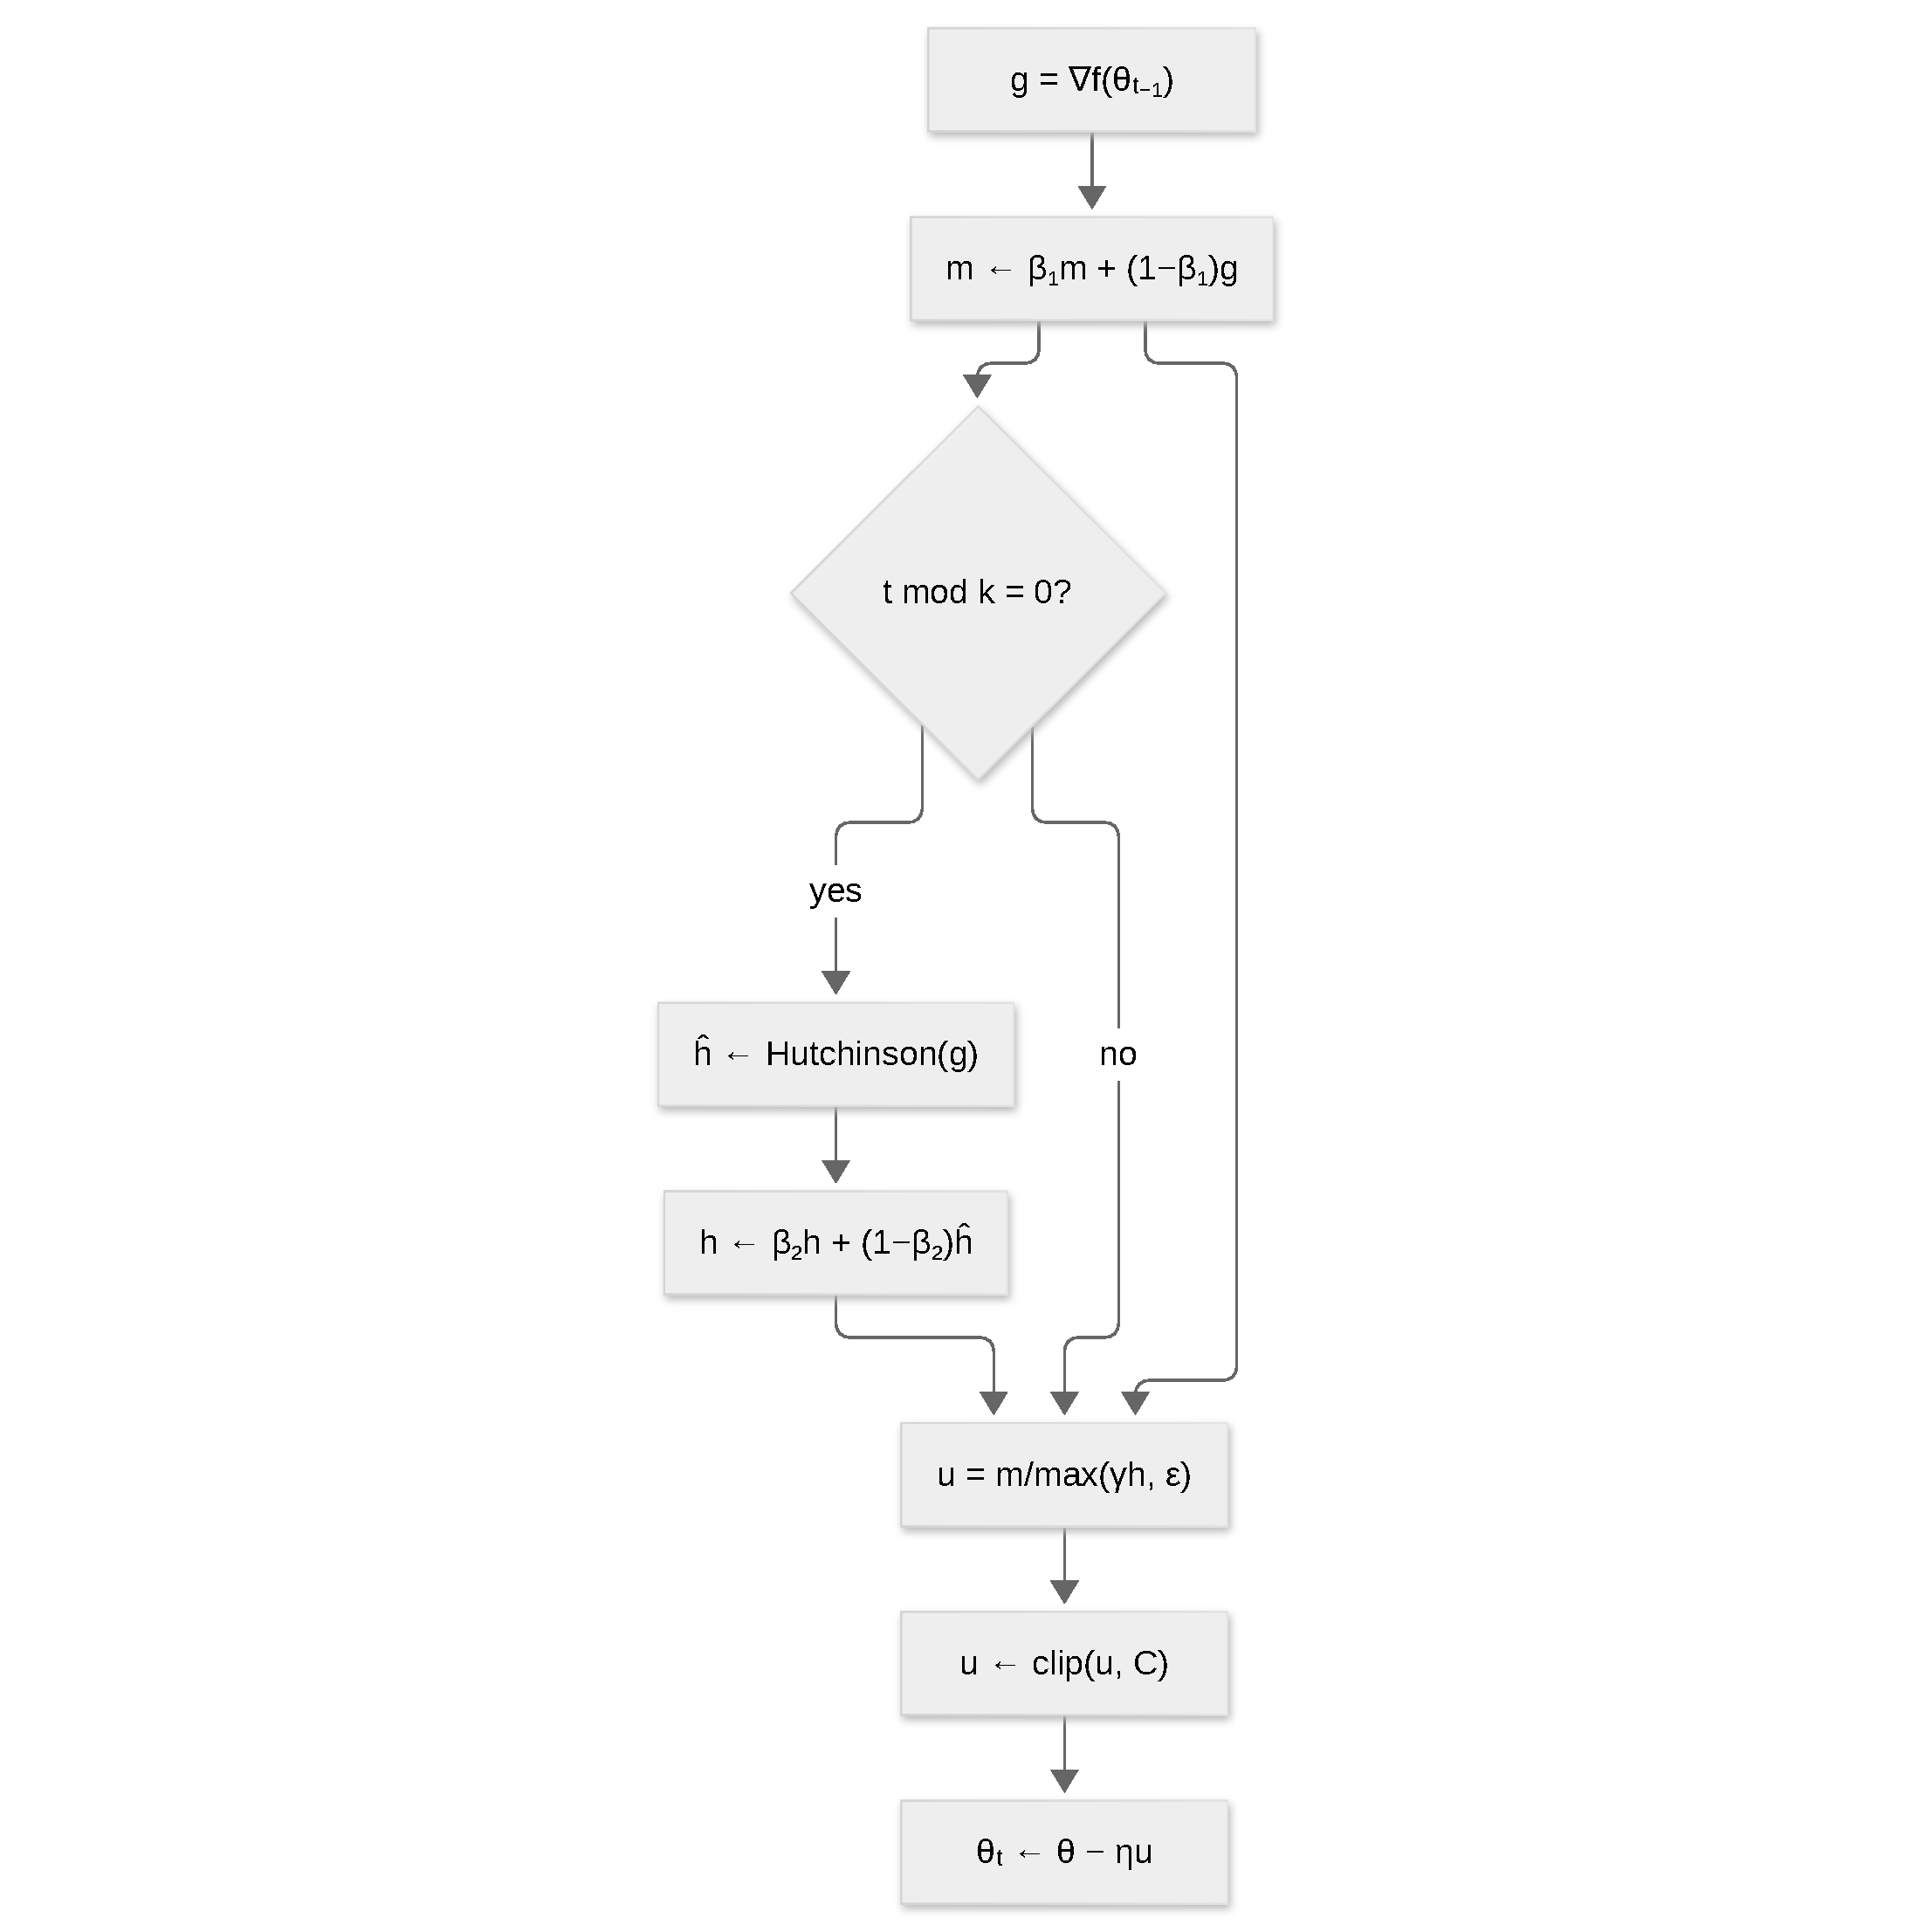
\includegraphics{../paper/figures/optimizers/sophia.pdf}}
\caption{Flujo por paso de Sophia: estimación diagonal del Hessiano mediante Hutchinson con pasos recortados conscientes de la curvatura.}
\label{fig:opt-sophia}
\end{figure}
Sophia utiliza \textbf{estimaciones diagonales del Hessiano} para escalado consciente de la curvatura sin el costo de memoria y cómputo de los métodos densos de segundo orden.
\begin{align}
m_t &= \beta_1 m_{t-1} + (1-\beta_1) g_t \quad\text{(momento de primer orden)} \\
h_t &= \beta_2 h_{t-(k-1)} + (1-\beta_2) \hat{h}_t \quad\text{(Hessiano diagonal, actualizado cada $k$ pasos)} \\
\text{clip}(x, C) &= \min(\max(x, -C), C) \quad\text{(recorte elemento a elemento)} \\
\theta_{t+1} &= \theta_t - \eta \cdot \text{clip}\left(\frac{m_t}{\max(\gamma h_t, \epsilon)}, 1\right)
\end{align}
donde $\hat{h}_t$ es una estimación diagonal (e.g., estimador de traza de Hutchinson) y $\gamma$ es un factor de escala. El Hessiano diagonal $h_t$ captura la curvatura local, permitiendo que el optimizador tome pasos más pequeños en direcciones pronunciadas y pasos más grandes en direcciones planas. La operación de recorte $\text{clip}(\cdot, 1)$ evita que los pasos adaptativos exploten.

\begin{algorithm}[H]
\caption{Sophia (Hessiano Diagonal con Actualizaciones Recortadas)}
\label{alg:sophia}
\begin{algorithmic}[1]
\Require Parámetros iniciales $\theta_0$, tasa de aprendizaje $\eta$, $\beta_1, \beta_2$, frecuencia de actualización del Hessiano $k$, umbral de recorte $C$
\Ensure Parámetros actualizados $\theta_T$
\State Inicializar: $m \gets 0$, $h \gets \epsilon$ (estimación diagonal del Hessiano)
\For{$t = 1, 2, \ldots, T$}
    \State $g \gets \nabla f(\theta_{t-1})$
    \State $m \gets \beta_1 m + (1-\beta_1) g$ \Comment{Momento de primer orden (corregir sesgo externamente)}
    \If{$t \mod k == 0$}
        \State $\hat{h} \gets \text{HutchinsonEstimate}(g)$ \Comment{Hessiano diagonal mediante Hutchinson}
        \State $h \gets \beta_2 h + (1-\beta_2) \hat{h}$ \Comment{Actualizar estimación del Hessiano}
    \EndIf
    \State $u \gets \frac{m}{\max(\gamma h, \epsilon)}$ \Comment{Paso adaptativo (elemento a elemento)}
    \State $u \gets \text{clip}(u, C)$ \Comment{Recorte elemento a elemento a $[-C, C]$}
    \State $\theta_t \gets \theta_{t-1} - \eta \cdot u$
\EndFor
\Return $\theta_T$
\end{algorithmic}
\end{algorithm}

\paragraph{Contras.}
\begin{itemize}[leftmargin=*]
\item Las estimaciones de Hutchinson añaden cómputo periódico y ruido a la señal de curvatura.
\item La estimación del Hessiano puede quedar desactualizada entre refrescos.
\end{itemize}

\paragraph{Ventajas.}
\begin{itemize}[leftmargin=*]
\item Escalado consciente de la curvatura sin el costo $O(n^2)$ u $O(n^3)$ de los métodos completos de segundo orden.
\item Los pasos recortados evitan explosiones y funcionan particularmente bien en el ajuste fino de segunda pasada.
\end{itemize}

\paragraph{Muon (Ortogonalización de Newton-Schulz).}
\begin{figure}[H]
\centering
\fitfigure{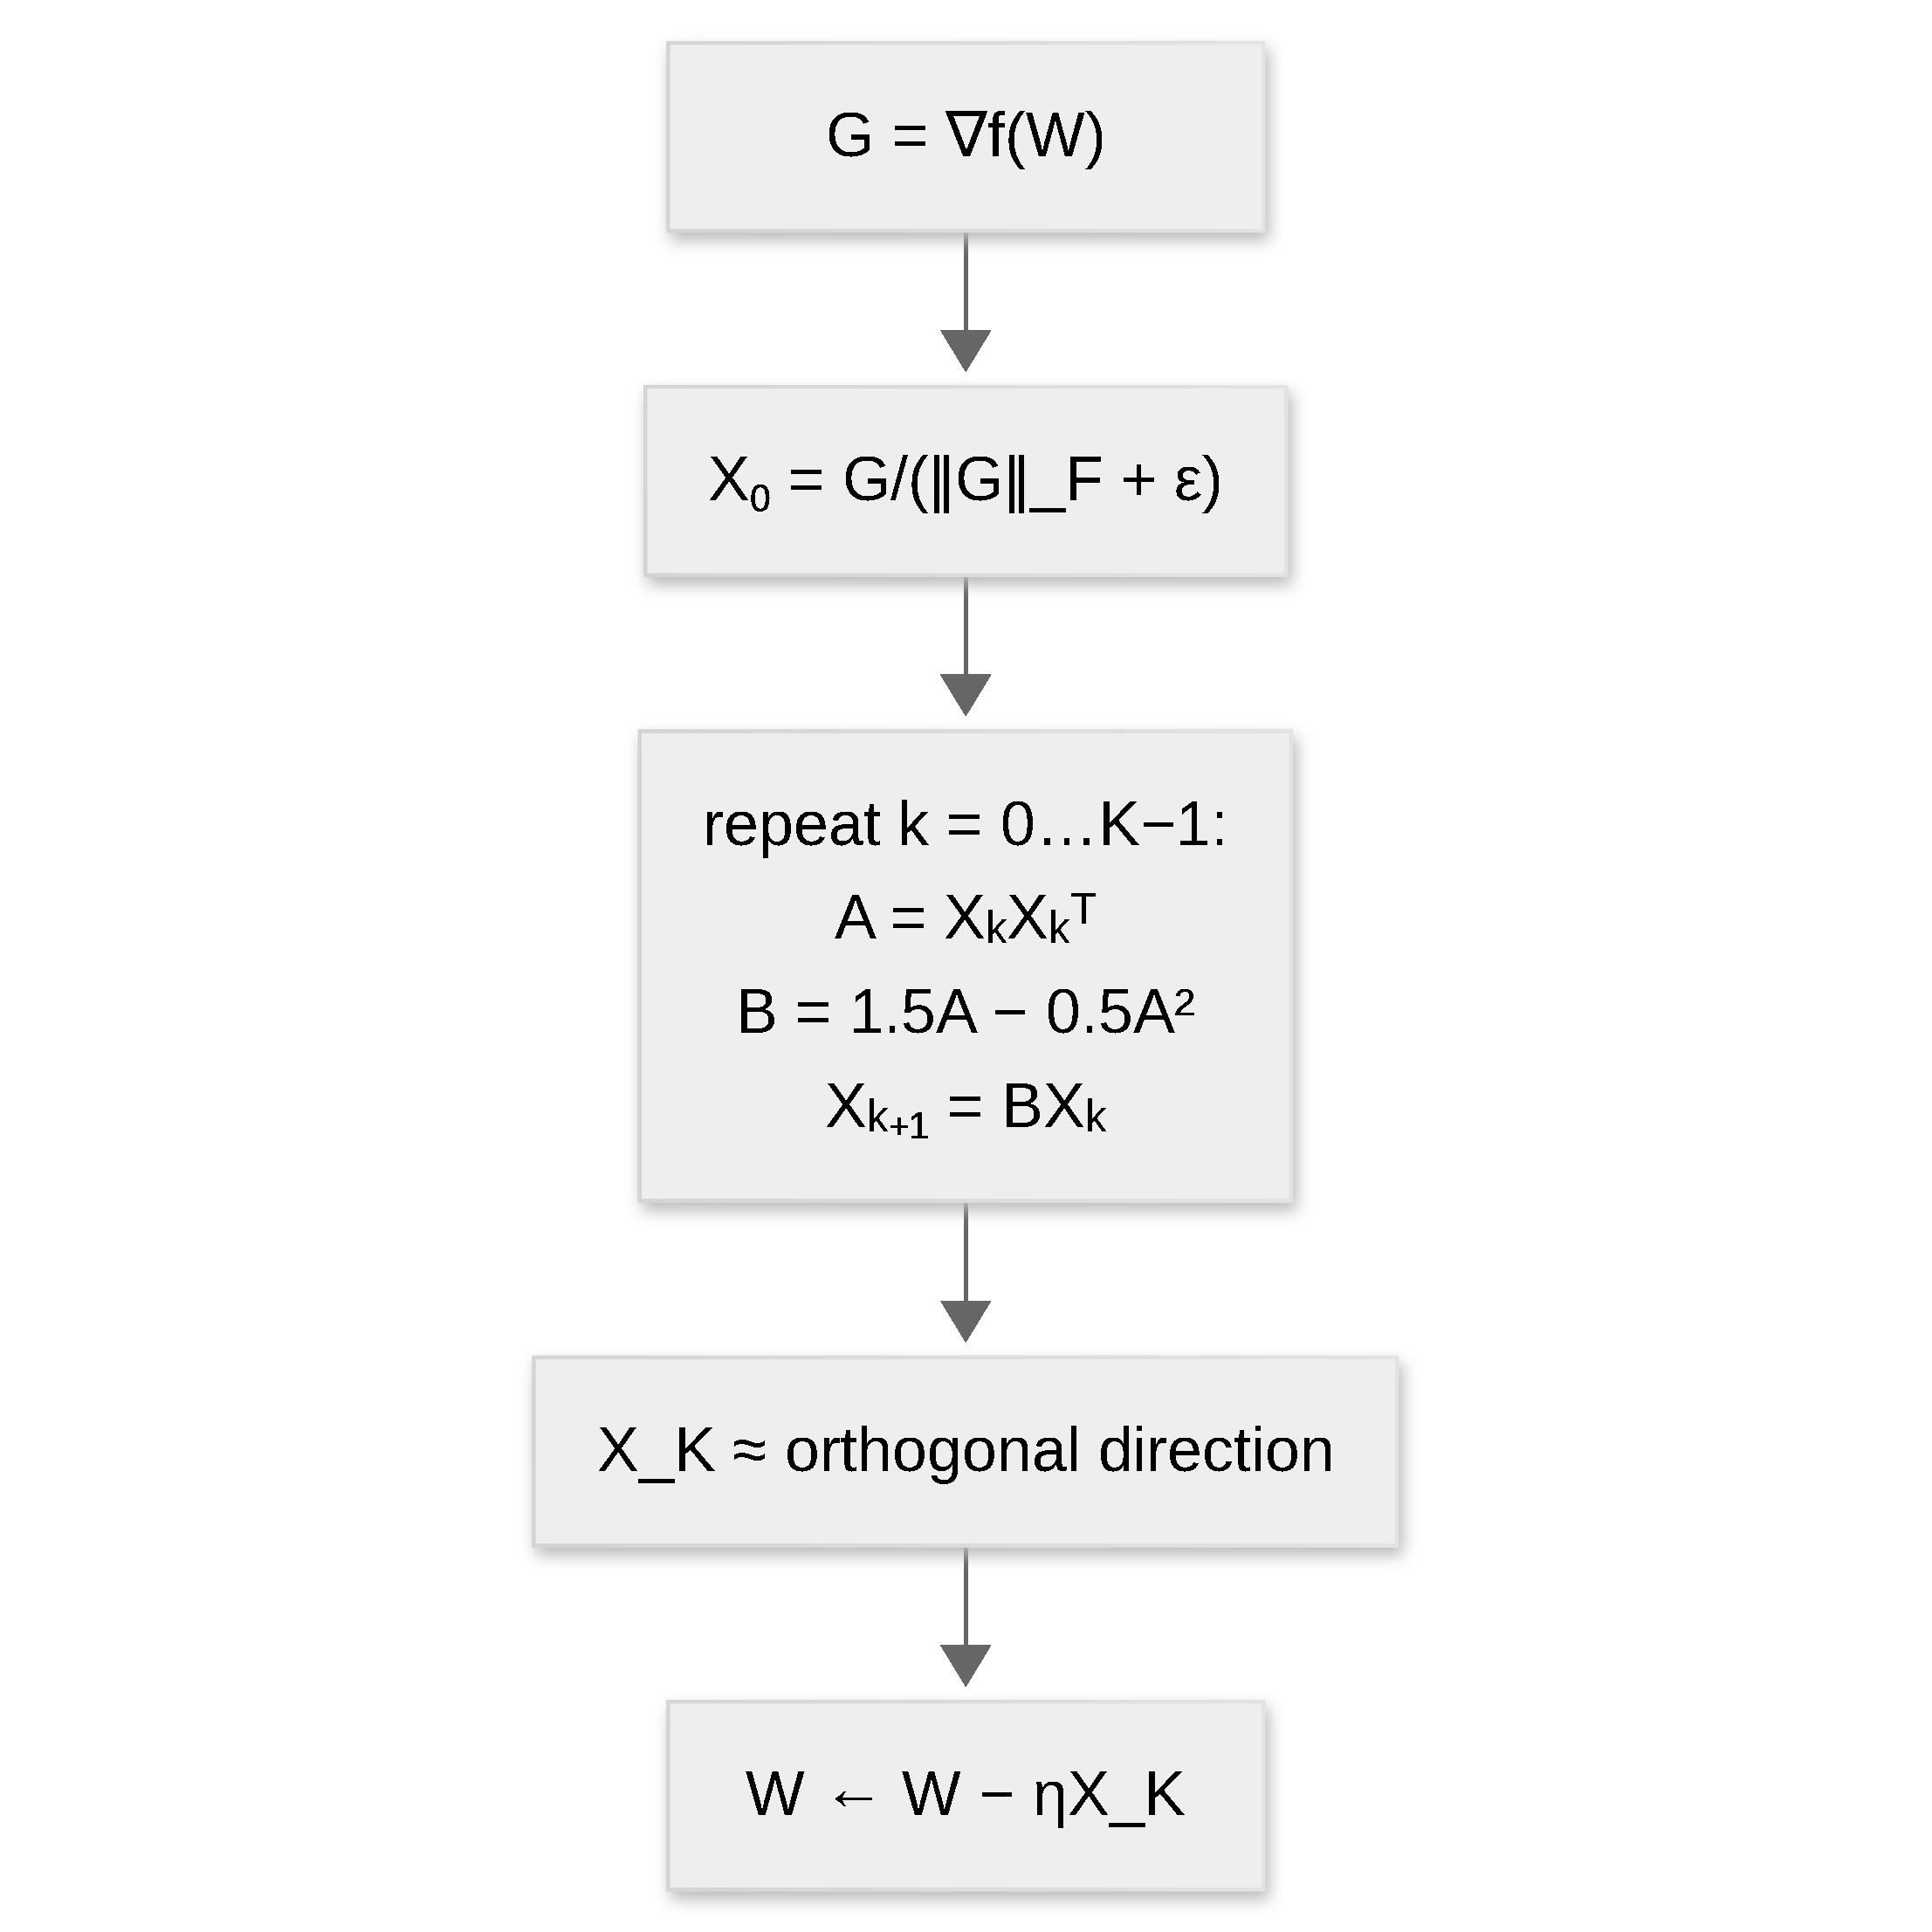
\includegraphics{../paper/figures/optimizers/muon.pdf}}
\caption{Flujo por paso de Muon: normalización de Frobenius seguida de iteraciones de Newton-Schulz que ortogonalizan la dirección de actualización.}
\label{fig:opt-muon}
\end{figure}
Muon es un \textbf{optimizador orientado a la ortogonalidad} que reformula la geometría de actualización utilizando iteraciones polinomiales de Newton-Schulz para ortogonalización. Para una matriz de parámetros 2D $W$ con gradiente $G_t$:
\begin{align}
X_0 &= \frac{G_t}{\|G_t\|_F + \epsilon} \quad\text{(gradiente normalizado)} \\
A_k &= X_k X_k^\top \quad\text{(Gramiana)} \\
B_k &= b A_k + c A_k^2 \quad\text{(paso polinomial, coeficientes $b, c$ de Newton-Schulz)} \\
X_{k+1} &= a X_k + B_k X_k \quad\text{(iteración $k=0,1,\ldots,4$)} \\
W_{t+1} &= W_t - \eta X_K \quad\text{(actualización con dirección ortogonalizada)}
\end{align}
Muon realiza 5 iteraciones de Newton-Schulz para producir una dirección aproximadamente ortogonal, asegurando que las actualizaciones respeten restricciones geométricas. La justificación: las actualizaciones ortogonales preservan las normas durante el entrenamiento, evitando la deriva de norma observada en métodos basados en momento.

\begin{algorithm}[H]
\caption{Muon (Ortogonalización de Newton-Schulz)}
\label{alg:muon}
\begin{algorithmic}[1]
\Require Parámetros iniciales $\theta$ (matrices), tasa de aprendizaje $\eta$, iteraciones Newton-Schulz $K$
\Ensure Parámetros actualizados $\theta_T$
\For{cada matriz de parámetros 2D $W$}
    \State $G \gets \nabla f(W)$ \Comment{Gradiente}
    \State $X_0 \gets \frac{G}{\|G\|_F + \epsilon}$ \Comment{Normalizar gradiente por norma de Frobenius}
    \For{$k = 0, 1, \ldots, K-1$}
        \State $A_k \gets X_k X_k^\top$ \Comment{Gramiana (costo: $O(mn^2)$ o $O(m^2n)$ para matrices altas/anchas)}
        \State $B_k \gets (3/2) A_k - (1/2) A_k^2$ \Comment{Coeficientes de Newton-Schulz}
        \State $X_{k+1} \gets B_k X_k$ \Comment{Paso polinomial}
    \EndFor
    \State $W \gets W - \eta X_K$ \Comment{Actualizar con dirección ortogonalizada}
\EndFor
\Return $\theta_T$
\end{algorithmic}
\end{algorithm}

\paragraph{Contras.}
\begin{itemize}[leftmargin=*]
\item Varias multiplicaciones de matrices por iteración de Newton-Schulz; se requieren kernels personalizados eficientes.
\item Definido solo para matrices de parámetros 2D.
\end{itemize}

\paragraph{Ventajas.}
\begin{itemize}[leftmargin=*]
\item Las actualizaciones ortogonalizadas preservan las normas y evitan la deriva de norma de los métodos basados en momento.
\item Resultados prometedores en entrenamiento a gran escala con una geometría de actualización fundamentalmente mejor condicionada.
\end{itemize}

\paragraph{Turbo-Muon (Ortogonalización Precondicionada con AOL).}
\begin{figure}[H]
\centering
\fitfigure{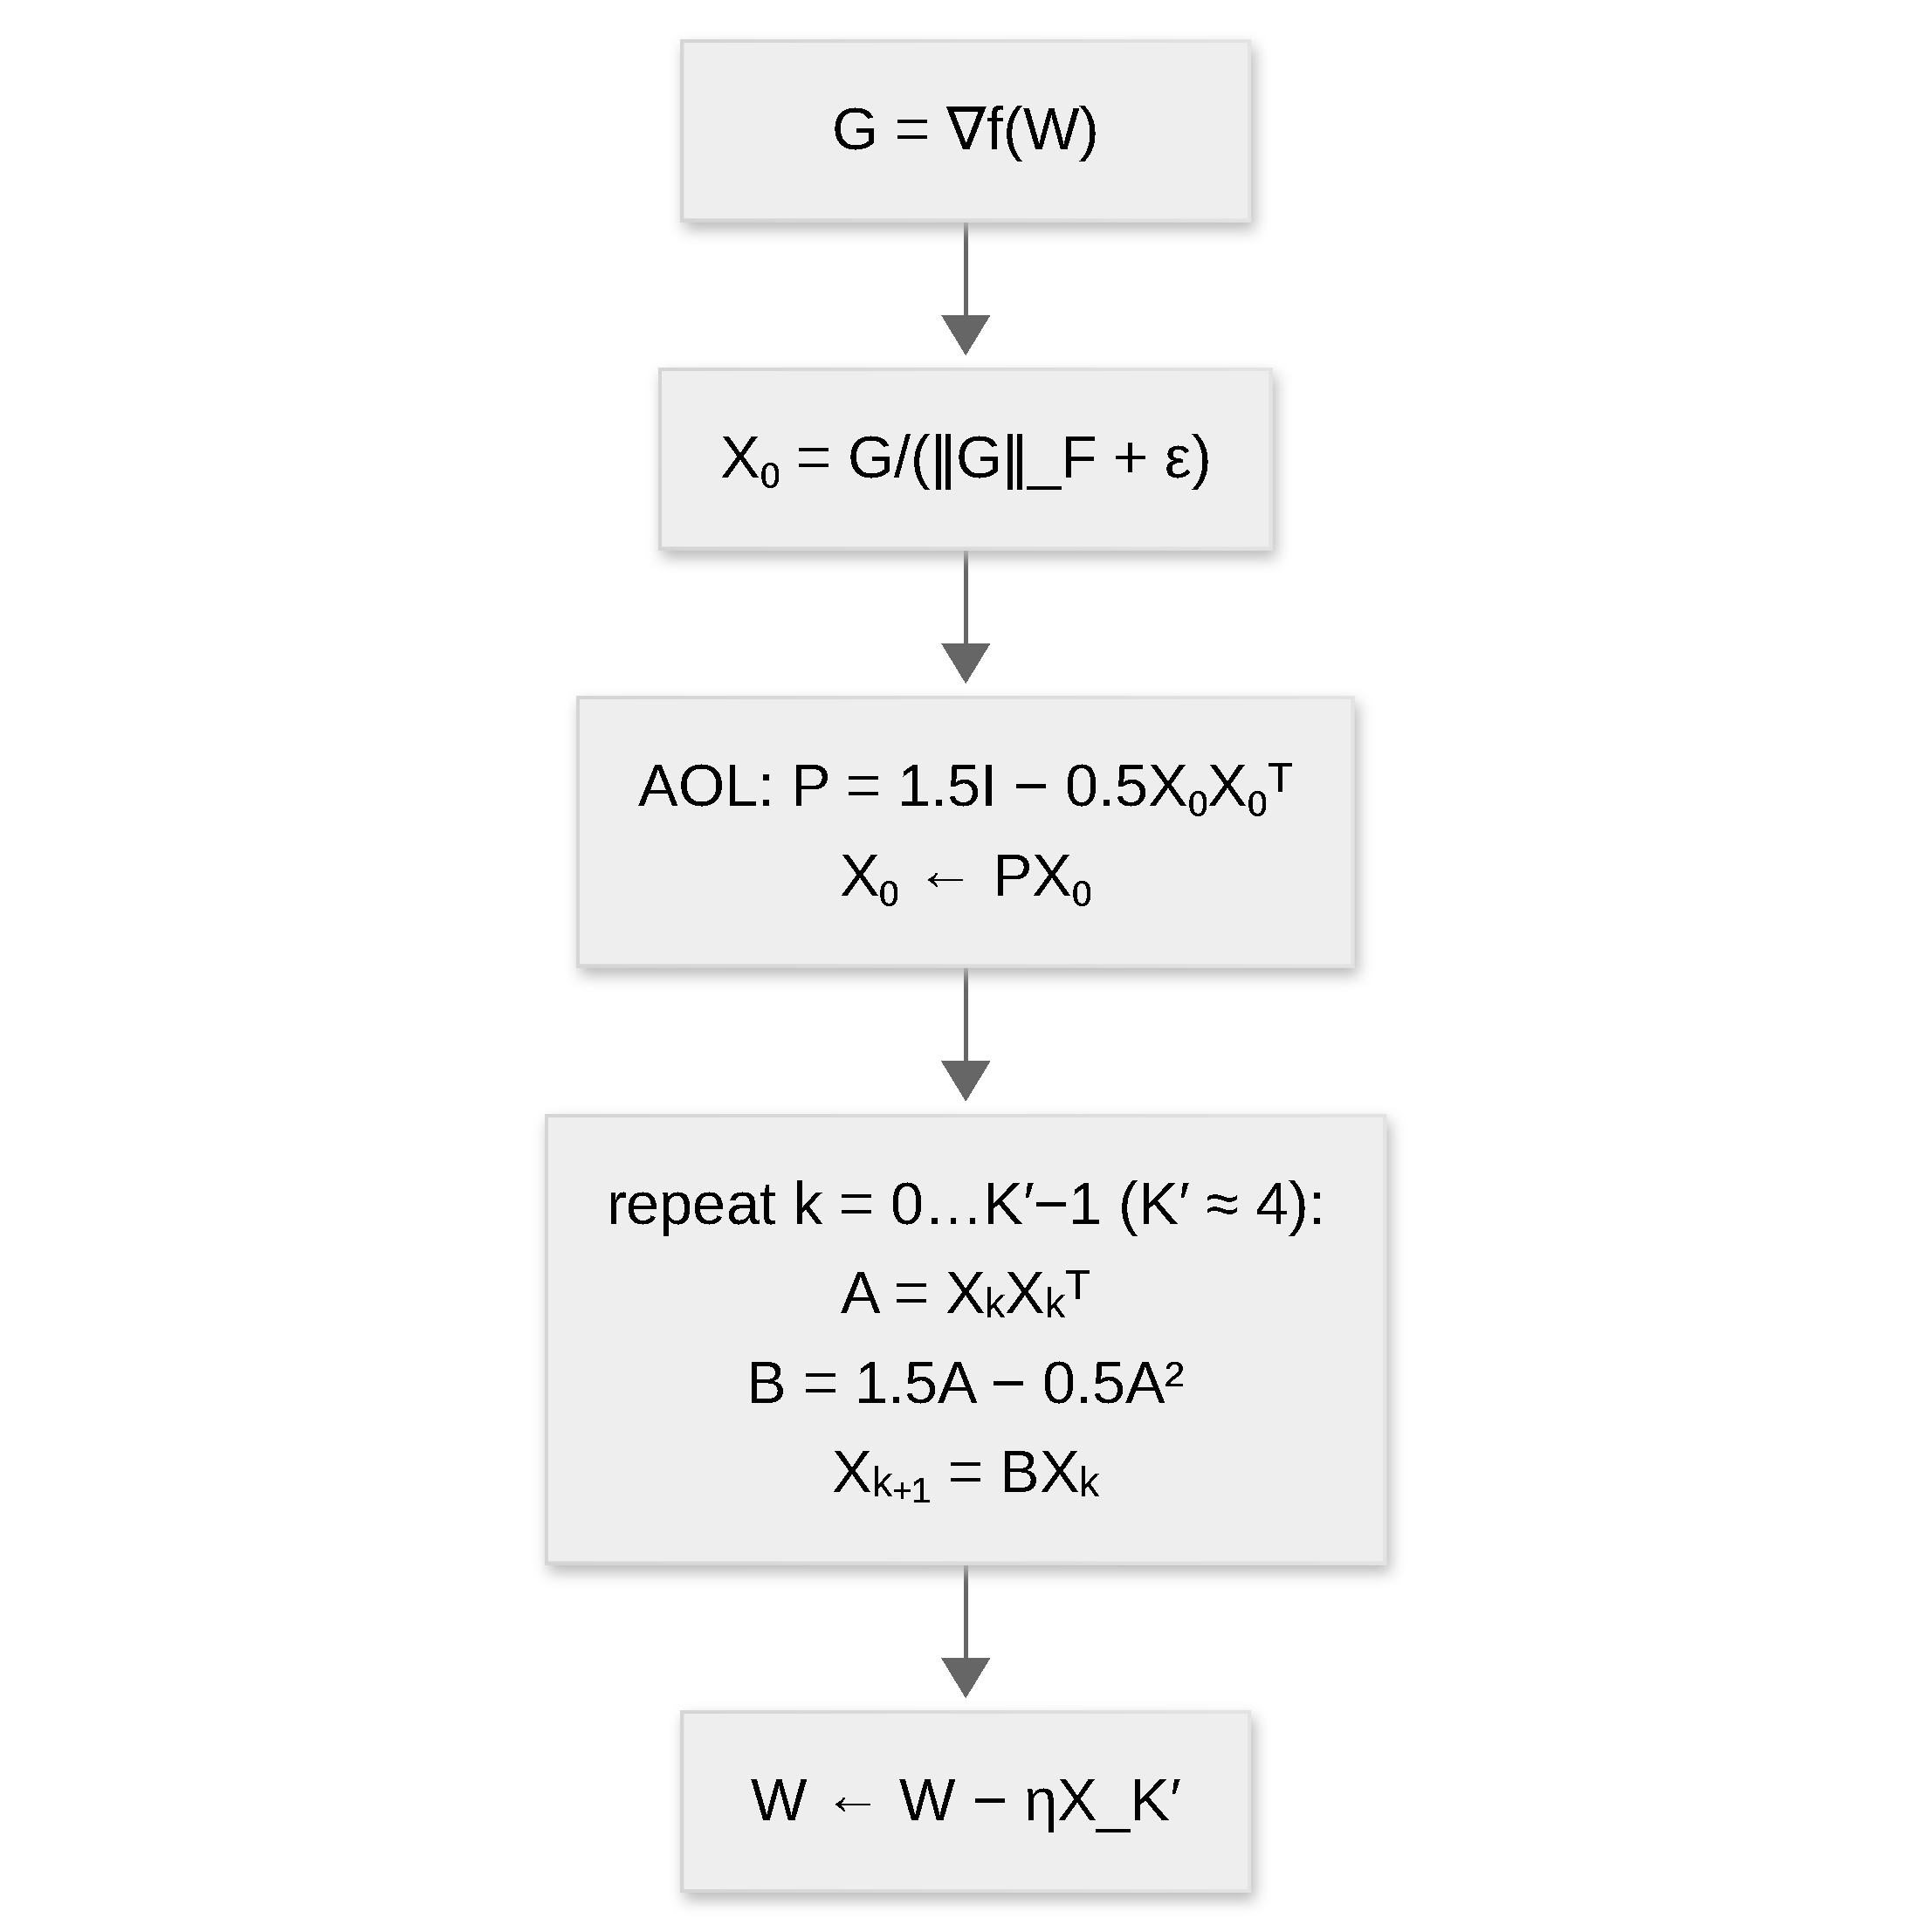
\includegraphics{../paper/figures/optimizers/turbo-muon.pdf}}
\caption{Flujo por paso de Turbo-Muon: precondicionamiento casi ortogonal (AOL) antes de las iteraciones de Newton-Schulz, reduciendo su número.}
\label{fig:opt-turbo-muon}
\end{figure}
Turbo-Muon añade un paso de \textbf{precondicionamiento casi-ortogonal} (AOL) antes de las iteraciones de Newton-Schulz. El precondicionador $P = 1.5I - 0.5X_0X_0^\top$ se aplica al gradiente normalizado, reduciendo el número de pasos de ortogonalización requeridos a cuatro mientras preserva la geometría de actualización ortogonalizada.

\begin{algorithm}[H]
\caption{Turbo-Muon (Ortogonalización Precondicionada con AOL)}
\label{alg:turbo-muon}
\begin{algorithmic}[1]
\Require Parámetros iniciales $\theta$ (matrices), tasa de aprendizaje $\eta$, iteraciones Newton-Schulz $K'$ (típicamente 4)
\Ensure Parámetros actualizados $\theta_T$
\For{cada matriz de parámetros 2D $W$}
    \State $G \gets \nabla f(W)$ \Comment{Gradiente}
    \State $X_0 \gets \frac{G}{\|G\|_F + \epsilon}$ \Comment{Normalizar gradiente}
    \State \textbf{AOL (Almost-Orthogonal preconditioner):} \Comment{Paso de precondicionamiento}
    \State $P \gets (1.5 I - 0.5 X_0 X_0^\top)$ \Comment{Matriz de precondicionamiento}
    \State $X_0 \gets P X_0$ \Comment{Inicio precondicionado}
    \For{$k = 0, 1, \ldots, K'-1$}
        \State $A_k \gets X_k X_k^\top$
        \State $B_k \gets (3/2) A_k - (1/2) A_k^2$
        \State $X_{k+1} \gets B_k X_k$ \Comment{Iteraciones reducidas gracias al precondicionamiento AOL}
    \EndFor
    \State $W \gets W - \eta X_{K'}$ \Comment{Actualizar con dirección ortogonalizada precondicionada}
\EndFor
\Return $\theta_T$
\end{algorithmic}
\end{algorithm}

\paragraph{Contras.}
\begin{itemize}[leftmargin=*]
\item Sigue siendo intensivo en cómputo; AOL añade una multiplicación de matrices de precondicionamiento.
\item Requiere el mismo soporte de kernels personalizados que Muon.
\end{itemize}

\paragraph{Ventajas.}
\begin{itemize}[leftmargin=*]
\item AOL reduce el número de iteraciones de Newton-Schulz (típicamente de cinco a cuatro).
\item Conserva la geometría de actualización ortogonalizada con menor costo de iteraciones.
\end{itemize}

\paragraph{AF-Muon (Muon sin AdamW para Vocabulario Atado).}
\begin{figure}[H]
\centering
\fitfigure{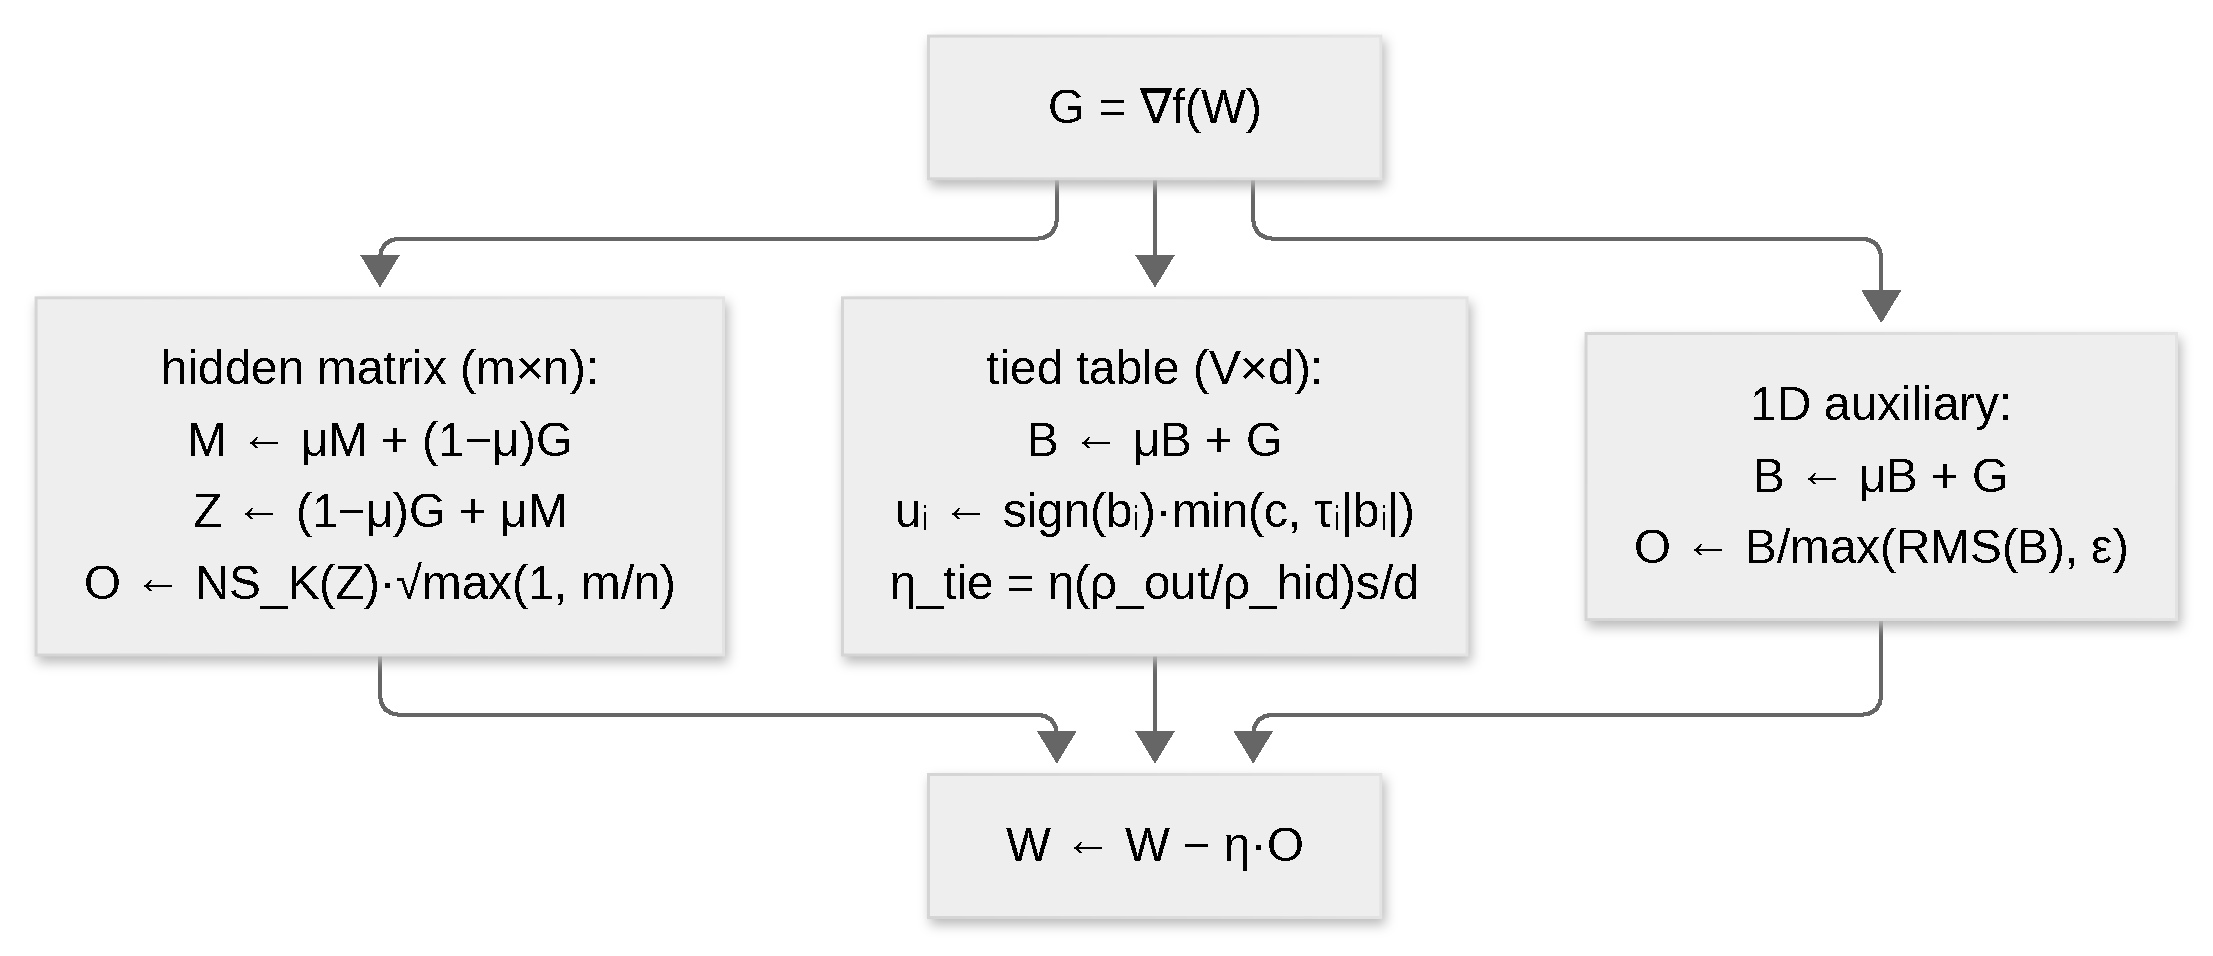
\includegraphics{../paper/figures/optimizers/af-muon.pdf}}
\caption{Flujo por paso de AF-Muon: actualización espectral de Muon para matrices ocultas, LMO por fila con tope finito y conciencia de soporte para la tabla de vocabulario atada, y actualizaciones normalizadas por RMS para parámetros auxiliares unidimensionales, todo con un único búfer de primer momento.}
\label{fig:opt-af-muon}
\end{figure}
AF-Muon es una \textbf{extensión de Muon sin AdamW} que elimina el respaldo auxiliar de AdamW de la receta Hybrid Muon asignando a cada clase de parámetro su propia geometría con restricción de norma. Las matrices ocultas conservan la actualización espectral con señal de Nesterov; la tabla de vocabulario, que recibe simultáneamente gradientes dispersos de búsqueda en la entrada y gradientes densos del softmax de salida, se actualiza fila por fila con un \emph{oráculo de minimización lineal con tope finito y conciencia de soporte}; los tensores auxiliares unidimensionales reciben una actualización normalizada por RMS. Ninguna clase de parámetro mantiene estado de segundo momento, de modo que un único búfer de primer momento por parámetro reemplaza el estado de AdamW de la receta híbrida, lo que los autores reportan como aproximadamente un 20\% menos de memoria de estado del optimizador en entrenamiento equiparado.

Para la tabla atada $W \in \mathbb{R}^{V \times d}$ con fila de momento $b_i$, el oráculo resuelve el problema por fila
\begin{align}
u_i &= \operatorname{sign}(b_i) \odot \min\left(c\,\mathbf{1},\ \tau_i\,|b_i|\right), \\
\|u_i\|_2^2 &= \min\left(d,\ c^2\,\bigl|\operatorname{supp}(b_i)\bigr|\right),
\end{align}
donde la escala por fila $\tau_i$ se obtiene por bisección en FP32 sobre fragmentos de filas completas. Las filas cuyo soporte no puede llenar el radio $\ell_2$ de fila saturan cada coordenada útil en el tope $c$, de modo que las filas dispersas de búsqueda se manejan sin inflar las coordenadas ausentes. El tope interpola entre dos extremos conocidos: $c = 1$ recupera la actualización Sign estilo SCION y $c \geq \sqrt{d}$ se reduce a una actualización row-RMS. El tamaño de paso de la tabla es $\eta_{tie} = \eta_M (\rho_{out}/\rho_{hid})\, s / d$; la configuración principal del artículo es $c = 3$ y $s = 0.5$ con $\rho_{out}/\rho_{hid} = 60$, y sus diagnósticos reportan el tope finito activo en menos del 0.3\% de las coordenadas aunque afecta a la mayoría de las filas.

\begin{algorithm}[H]
\caption{AF-Muon (Muon sin AdamW para Vocabulario Atado)}
\label{alg:af-muon}
\begin{algorithmic}[1]
\Require Parámetros iniciales $\theta$, LR de matrices $\eta_M$, LR de vectores $\eta_{vec}$, momento $\mu$, weight decay de matrices $\lambda_M$, escala de tabla $s$, tope $c$, radios $\rho_{out}, \rho_{hid}$, iteraciones Newton-Schulz $K$
\Ensure Parámetros actualizados $\theta_T$
\For{cada tensor de parámetros $W$ con gradiente $G_t$}
    \If{$W$ es una matriz oculta en $\mathbb{R}^{m \times n}$}
        \State $M_t \gets \mu M_{t-1} + (1-\mu) G_t$ \Comment{Primer momento}
        \State $Z_t \gets (1-\mu) G_t + \mu M_t$ \Comment{Señal de Nesterov}
        \State $O_t \gets \mathrm{NS}_K(Z_t)\sqrt{\max(1, m/n)}$ \Comment{Actualización espectral}
        \State $W_t \gets (1 - \eta_M \lambda_M) W_{t-1} - \eta_M O_t$
    \ElsIf{$W \in \mathbb{R}^{V \times d}$ es la tabla de vocabulario atada}
        \State $B_t \gets \mu B_{t-1} + G_t$ \Comment{Primer momento sin normalizar}
        \State $\eta_{tie,t} \gets \eta_M (\rho_{out}/\rho_{hid}) s / d$
        \For{cada fila $i = 1, \ldots, V$}
            \State $u_i \gets L_c\bigl(\mathrm{fila}_i(B_t)\bigr)$ \Comment{LMO por fila con tope}
        \EndFor
        \State $W_t \gets W_{t-1} - \eta_{tie,t} U$
    \Else
        \State $B_t \gets \mu B_{t-1} + G_t$ \Comment{Tensor auxiliar 1D}
        \State $O_t \gets B_t / \max(\mathrm{RMS}(B_t), \epsilon)$
        \State $W_t \gets W_{t-1} - \eta_{vec} O_t$
    \EndIf
\EndFor
\Return $\theta_T$
\end{algorithmic}
\end{algorithm}

\paragraph{Contras.}
\begin{itemize}[leftmargin=*]
\item Cada parámetro debe recibir un rol explícito (matriz, tabla atada o vector); un head de salida no atado o una tabla de embeddings adicional no son bloques de tabla atada.
\item El oráculo de la tabla requiere bisección por fila con fragmentación de filas completas; el artículo reporta aproximadamente un 1\% de sobrecarga mediana por paso en entrenamiento equiparado.
\item La afirmación sobre la tabla atada se establece para modelos con vocabulario atado; no se reclama preentrenamiento a escala frontera ni superioridad universal de los extremos.
\end{itemize}

\paragraph{Ventajas.}
\begin{itemize}[leftmargin=*]
\item Sin AdamW: un búfer de primer momento por parámetro y sin estado de segundo momento, reportado como aproximadamente un 20\% menos de memoria de estado del optimizador que Hybrid Muon.
\item El tope finito preserva las magnitudes intra-fila mientras acota la concentración de coordenadas, y recupera Sign ($c=1$) y row-RMS ($c \geq \sqrt{d}$) como casos límite.
\item Mejora la pérdida de validación y la perplejidad medias frente a Hybrid Muon y a un extremo Sign estilo SCION en nueve configuraciones de vocabulario atado que abarcan texto, tokens de imagen, proteínas, MoE y modelos encoder-decoder.
\end{itemize}

\paragraph{AdaMuon (Muon Adaptativo).}
AdaMuon es una \textbf{extensión adaptativa de Muon} que conserva la actualización espectral (polar) y añade normalización de varianza por coordenada. Muon ortogonaliza la matriz de momentum en una actualización puramente direccional, lo que elimina el escalado anisotrópico pero asigna la misma magnitud a todas las coordenadas; AdaMuon aborda el desajuste resultante entre coordenadas ruidosas e informativas siguiendo la varianza por elemento de la dirección \emph{ortogonalizada}, en lugar de la del gradiente crudo o la del momentum. Como el factor polar es globalmente invariante a escala, la transformación de signo aplicada antes de la ortogonalización preserva la dirección de la actualización mientras estabiliza sus magnitudes por elemento; el artículo demuestra que $\operatorname{sign}$ es la única aplicación elemental que es libre de escala, consistente con el signo, impar y acotada (Teorema~1). La estimación de segundo momento ve así una señal estable, y su versión normalizada por varianza se reescala a un RMS de $0.2$, igualando la escala empírica de actualización de Adam para reutilizar sin ajuste los schedules de tasa de aprendizaje existentes.

Para un peso $W_t \in \mathbb{R}^{n \times m}$, búfer de momentum $M_t$, momentum $\beta$, pasos de Newton--Schulz $T$ y constante pequeña $\varepsilon$:
\begin{align}
M_t &= \beta M_{t-1} + G_t, \\
O_t &= \operatorname{NewtonSchulz}\bigl(\operatorname{sign}(M_t), T\bigr), \\
V_t &= \beta V_{t-1} + (1-\beta)\, O_t \odot O_t, \\
\widehat{O}_t &= O_t \oslash \bigl(\sqrt{V_t} + \varepsilon \mathbf{1}\bigr), \\
\gamma_t &= \frac{0.2\sqrt{mn}}{\|\widehat{O}_t\|_F}, \\
W_{t+1} &= W_t - \eta\bigl(\gamma_t \widehat{O}_t + \lambda W_t\bigr).
\end{align}
El mapa de Newton--Schulz usa $X_0 = \operatorname{sign}(M_t)/\|\operatorname{sign}(M_t)\|_F$ y la iteración cúbica $X_k = aX_{k-1} + b(X_{k-1}X_{k-1}^{\mathsf T})X_{k-1} + c(X_{k-1}X_{k-1}^{\mathsf T})^2X_{k-1}$ con $(a,b,c) = (3.4445, -4.7750, 2.0315)$ y $T = 5$. No se aplica corrección de sesgo a ninguno de los momentos: un factor constante en $V_t$ se cancela exactamente con $\gamma_t \propto \sqrt{c}$, y un factor constante en $M_t$ se elimina con el mapa polar, $\operatorname{polar}(cM) = \operatorname{polar}(M)$.

\begin{algorithm}[H]
\caption{AdaMuon (Muon Adaptativo)}
\label{alg:ada-muon}
\begin{algorithmic}[1]
\Require Pesos iniciales $W_0 \in \mathbb{R}^{n \times m}$, tasa de aprendizaje $\eta$, weight decay $\lambda$, momentum $\beta$, pasos de Newton--Schulz $T$, constante pequeña $\varepsilon$
\Ensure Pesos actualizados $W_T$
\State $M_0 \gets \mathbf{0}$, $V_0 \gets \mathbf{0}$
\For{cada iteración $t = 1, 2, \ldots$}
    \State $G_t \gets \nabla_{W_t}\mathcal{L}(W_t)$
    \State $M_t \gets \beta M_{t-1} + G_t$
    \State $O_t \gets \operatorname{NewtonSchulz}(\operatorname{sign}(M_t), T)$
    \State $V_t \gets \beta V_{t-1} + (1-\beta)\, O_t \odot O_t$
    \State $\widehat{O}_t \gets O_t \oslash (\sqrt{V_t} + \varepsilon\mathbf{1})$
    \State $\gamma_t \gets 0.2\sqrt{mn}/\|\widehat{O}_t\|_F$
    \State $W_{t+1} \gets W_t - \eta(\gamma_t \widehat{O}_t + \lambda W_t)$
\EndFor
\Return $W_T$
\end{algorithmic}
\end{algorithm}

\paragraph{Contras.}
\begin{itemize}[leftmargin=*]
\item Un búfer de segundo momento adicional por parámetro matricial (dos búferes frente al único búfer de primer momento de Muon), más trabajo por paso de EMA elemental, raíz cuadrada y normalización sobre la actualización.
\item La actualización está definida para parámetros bidimensionales; los parámetros unidimensionales (sesgos, escalas de normalización) requieren un optimizador auxiliar en la receta del artículo.
\item El objetivo RMS ($0.2$) es una constante fija y no una cantidad aprendida, por lo que el método asume escalas de actualización tipo Adam al reutilizar schedules existentes.
\end{itemize}

\paragraph{Ventajas.}
\begin{itemize}[leftmargin=*]
\item Sin hiperparámetros nuevos: la EMA de segundo momento reutiliza el coeficiente de momentum $\beta$ de Muon, y el artículo reporta baja sensibilidad para $\beta \in [0.8, 0.99]$.
\item La transformación de signo hace que la estimación de varianza sea lo bastante estable para normalizar, y la alineación RMS cancela cualquier sesgo constante en $V_t$, por lo que no se necesita corrección de sesgo para ninguno de los dos momentos.
\item La alineación RMS iguala la escala de actualización de Adam, lo que permite reutilizar directamente los schedules de tasa de aprendizaje; los autores reportan hasta aproximadamente un 40\% de ganancia en eficiencia de entrenamiento frente a AdamW y mejoras consistentes frente a Muon en GPT-2 (125M--1.5B) y Qwen2.5 (1.5B, 7B).
\end{itemize}

\small
\begin{longtable}{L{2.5cm}L{3.5cm}L{2.3cm}L{5.0cm}}
\toprule
\textbf{Grupo} & \textbf{Métodos} & \textbf{Objetivo Principal} & \textbf{Interpretación desde el Estudio} \\
\midrule
\endhead
Línea base clásica & SGD, AdamW, RAdam & estabilidad y referencias base & Definen el piso de comparación para las afirmaciones de optimizadores más nuevos. \\
Rediseño de momento & Adan, AdEMAMix, MARS, Cautious AdamW & adaptación de primer orden más rápida o segura & Mejor cuando la velocidad de convergencia o la estabilidad ante gradiente ruidoso es la preocupación principal. \\
Simplificación de lotes grandes y programación & LAMB, Schedule-Free AdamW & robustez operacional a escala & Reducen la fragilidad debida al crecimiento del tamaño de lote o la ingeniería de programación. \\
Eficiencia de memoria & Adafactor, GaLore, APOLLO, APOLLO-Mini, Q-APOLLO, Lion & reducción del estado del optimizador & Más útil cuando la VRAM está dominada por el estado del optimizador en lugar de las activaciones; los métodos de la familia APOLLO reemplazan los momentos densos de AdamW con escalado estructurado proyectado o cuantizado. \\
Consciente de curvatura & Shampoo, SOAP, Sophia & mejor condicionamiento & Preferir cuando una geometría más rica justifica la sobrecarga de implementación y cómputo. \\
Orientado a geometría & Muon, Turbo-Muon, AF-Muon, AdaMuon & estructura de actualización ortogonalizada & Opciones especializadas para geometría matricial y modelado de representaciones; AdaMuon añade un segundo momento por elemento sobre la dirección ortogonalizada con actualizaciones alineadas por RMS; AF-Muon asigna a la tabla de vocabulario atada una geometría de tabla con tope por fila y a los parámetros unidimensionales una actualización RMS, sin estado auxiliar de AdamW. \\
\bottomrule
\end{longtable}
\normalsize

\section{Transformadores Densos, Recurrentes y Aumentados con Memoria}
\label{sec:annex-transformer}

Este anexo sintetiza las familias densas, recurrentes y aumentadas con memoria de transformers. El campo ha evolucionado hacia varios paradigmas principales: atención densa global con variantes, compresión de cabezas clave-valor mediante atención por consultas agrupadas, compresión de estado recurrente con decaimiento, modelos de espacio de estado selectivos, integración numérica de profundidad continua y arquitecturas aumentadas con memoria. Comprender esta taxonomía ilumina las compensaciones fundamentales entre expresividad, costo computacional, huella de memoria y simplicidad de despliegue.

\subsection{Atención Densa de Referencia: Estándar y Sigmoide}

\subsubsection{Atención Softmax Estándar}

\begin{figure}[H]
\centering
\fitfigure{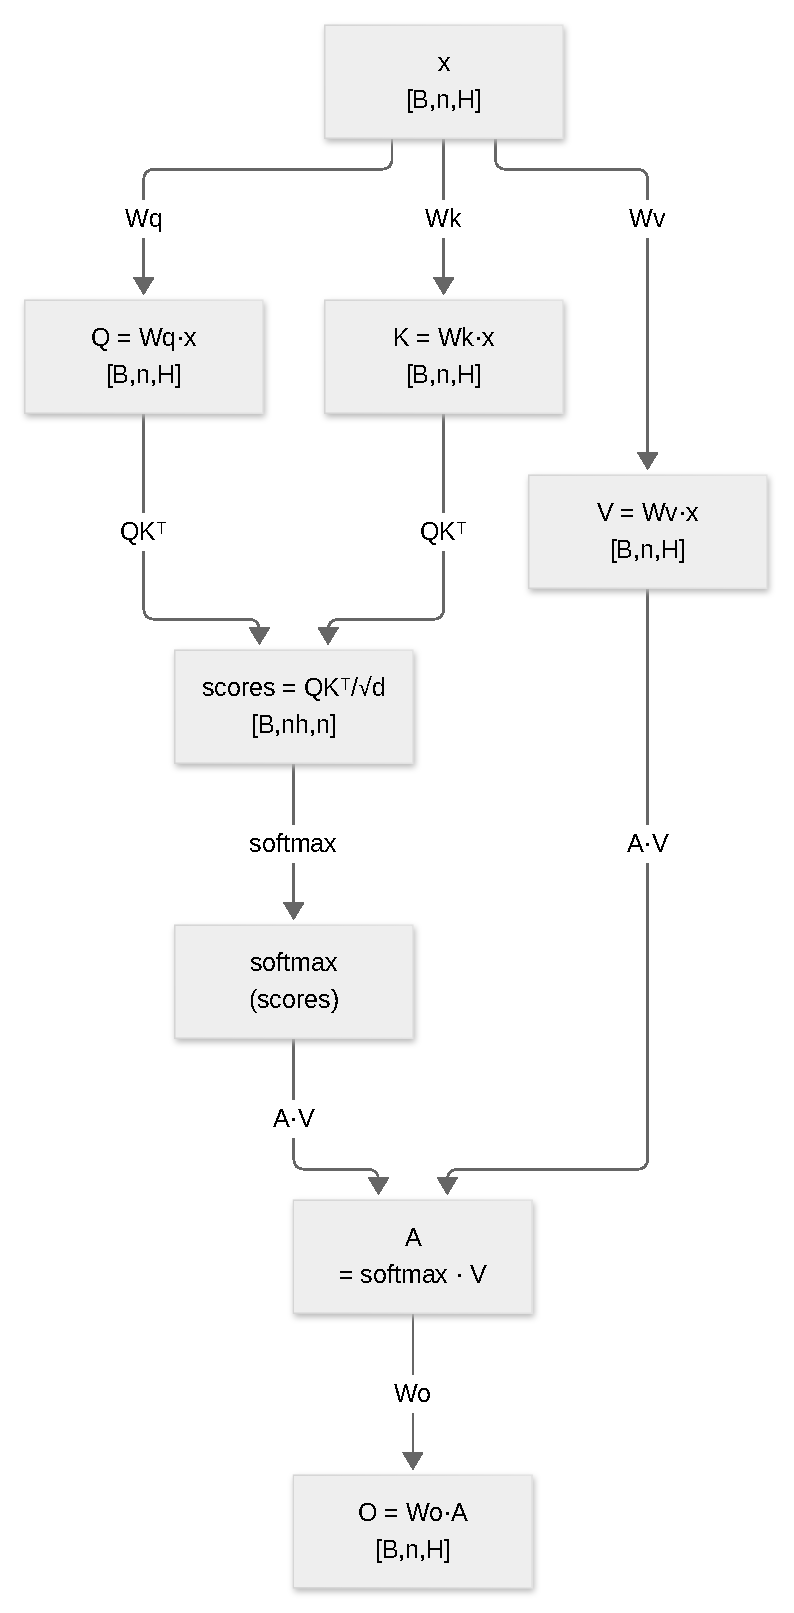
\includegraphics{../paper/figures/mixers/standard.pdf}}
\caption{Flujo de datos de la atención softmax estándar: proyecciones Q/K/V paralelas, puntuaciones de producto escalar escaladas, softmax por filas y proyección de salida.}
\label{fig:mixer-standard}
\end{figure}
La atención multi-cabeza estándar \citep{vaswani_attention_2017} calcula la similitud de producto punto escalado entre embeddings de tokens:

\begin{algorithmic}[1]
\State \textbf{Entrada:} Matriz de consulta $\mathbf{Q} \in \mathbb{R}^{n \times d}$, Matriz de clave $\mathbf{K} \in \mathbb{R}^{n \times d}$, Matriz de valor $\mathbf{V} \in \mathbb{R}^{n \times d}$
\State $\text{puntajes} \gets \frac{\mathbf{Q}\mathbf{K}^\top}{\sqrt{d}} \in \mathbb{R}^{n \times n}$ \Comment{calcular similitudes por pares}
\State $\text{pesos\_atencion} \gets \texttt{softmax}(\text{puntajes}, \text{eje}=1) \in \mathbb{R}^{n \times n}$ \Comment{normalizar sobre las claves}
\State \textbf{Salida:} $\mathbf{Y} = \text{pesos\_atencion} \cdot \mathbf{V} \in \mathbb{R}^{n \times d}$ \Comment{combinación ponderada de valores}
\end{algorithmic}

Para generación autorregresiva, el almacenamiento en caché KV guarda claves y valores pasados para evitar el recálculo $\mathcal{O}(n^2)$. Sin embargo, este caché de crecimiento lineal ocupa $\sim n \cdot d_{\text{oculto}}$ bytes, lo que puede consumir cientos de gigabytes para modelos de miles de millones de parámetros. La atención estándar logra una \textbf{expresividad perfecta} dentro de la ventana de contexto---cualquier token puede atender a cualquier otro token con pesos aprendidos---pero paga el precio del cómputo denso.

\begin{itemize}[leftmargin=*]
    \item \textbf{Complejidad de entrenamiento}: $\mathcal{O}(n^2 \cdot d)$ tiempo, $\mathcal{O}(n^2)$ espacio (materialización de la matriz de atención).
    \item \textbf{Complejidad de inferencia}: $\mathcal{O}(n)$ tiempo por token, $\mathcal{O}(n)$ espacio (caché KV).
    \item \textbf{Fortalezas}: Expresividad incomparable; recuperación perfecta del historial; altamente paralelizable.
    \item \textbf{Debilidades}: El cuello de botella cuadrático prohíbe contextos muy largos; el caché KV domina la memoria durante la generación.
\end{itemize}

\subsubsection{Atención Sigmoide}

\begin{figure}[H]
\centering
\fitfigure{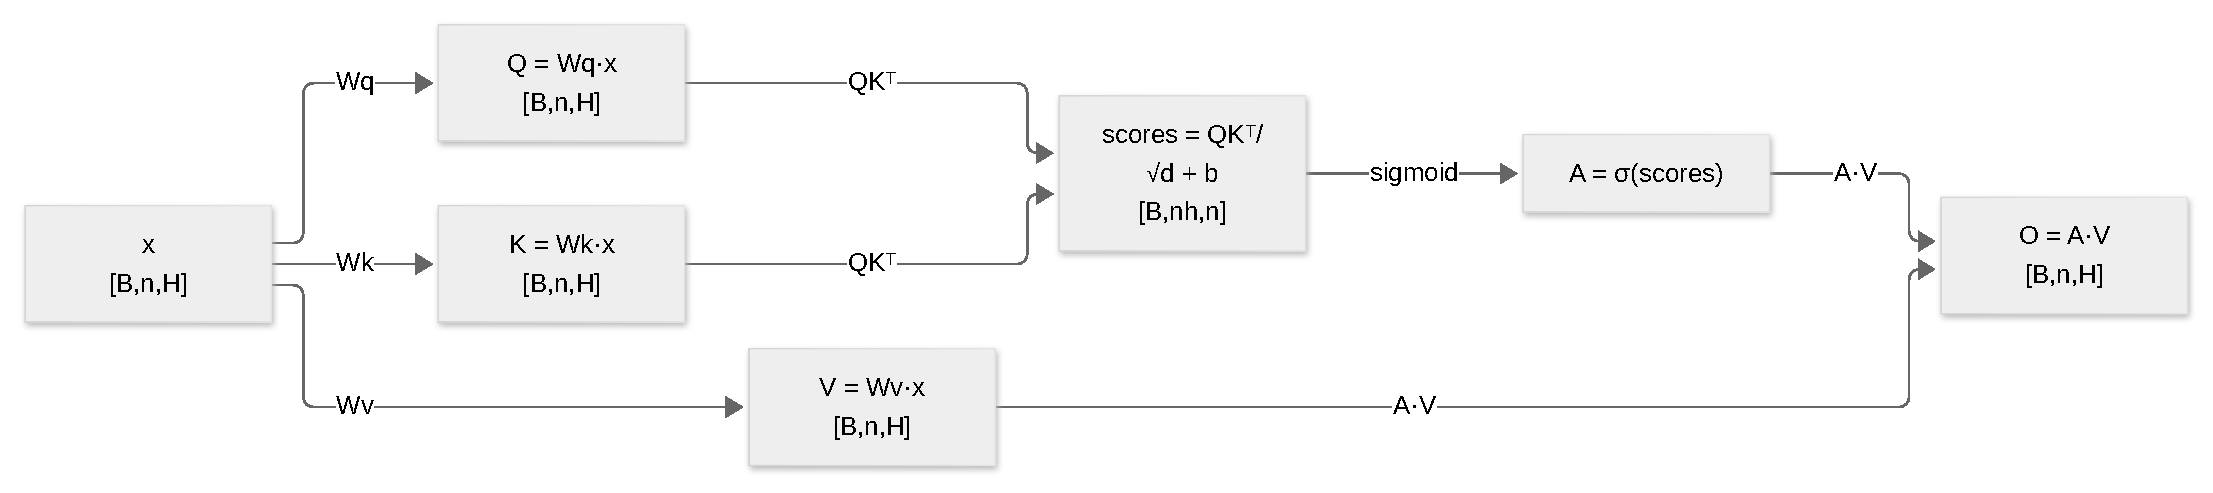
\includegraphics{../paper/figures/mixers/sigmoid.pdf}}
\caption{Flujo de datos de la atención sigmoide: una sigmoide elemento a elemento sustituye al softmax por filas, de modo que los pesos de atención no tienen por qué sumar uno.}
\label{fig:mixer-sigmoid}
\end{figure}
La atención sigmoide reemplaza el softmax por filas con una activación sigmoide elemento a elemento \citep{ramapuram_theory_2024}:

\begin{algorithmic}[1]
\State \textbf{Entrada:} $\mathbf{Q}, \mathbf{K}, \mathbf{V}$ como arriba, sesgo aprendible $\mathbf{b} \in \mathbb{R}^{n \times n}$
\State $\text{logits} \gets \frac{\mathbf{Q}\mathbf{K}^\top}{\sqrt{d}} + \mathbf{b}$
\State $\text{pesos\_atencion} \gets \sigma(\text{logits})$ \Comment{sigmoide elemento a elemento, no softmax}
\State \textbf{Salida:} $\mathbf{Y} = \text{pesos\_atencion} \odot \mathbf{V}$
\end{algorithmic}

A diferencia de softmax, la sigmoide no impone una distribución de probabilidad (los pesos no necesitan sumar 1), lo que permite una independencia de tokens más fuerte. El análisis teórico mediante mezcla de expertos muestra que la sigmoide alcanza una complejidad muestral superior: convergencia $\mathcal{O}(n^{-0.51})$ para expertos ReLU frente a $\mathcal{O}(n^{-0.24})$ de softmax. Sin embargo, el entrenamiento empírico reveló inestabilidades de gradiente a escala. El remedio es la \textbf{norma híbrida}---agregar normalización después de la salida de atención---que estabiliza los gradientes sin sacrificar los beneficios teóricos del enrutamiento elemento a elemento.

\begin{itemize}[leftmargin=*]
    \item \textbf{Complejidad de entrenamiento}: $\mathcal{O}(n^2 \cdot d)$ (idéntico al estándar), pero las operaciones elemento a elemento permiten una aceleración de inferencia del 17\% mediante FlashSigmoid.
    \item \textbf{Complejidad de inferencia}: $\mathcal{O}(n)$ por token con caché KV (asintóticamente igual, pero con factores constantes más bajos).
    \item \textbf{Fortalezas}: Supera la competencia de suma cero; evita la sincronización por filas; implementación eficiente en hardware.
    \item \textbf{Debilidades}: Requiere estabilización cuidadosa (norma híbrida); inestabilidad de entrenamiento a grandes escalas sin pérdida auxiliar.
\end{itemize}

\subsubsection{Atención por Consultas Agrupadas (GQA)}

\begin{figure}[H]
\centering
\fitfigure{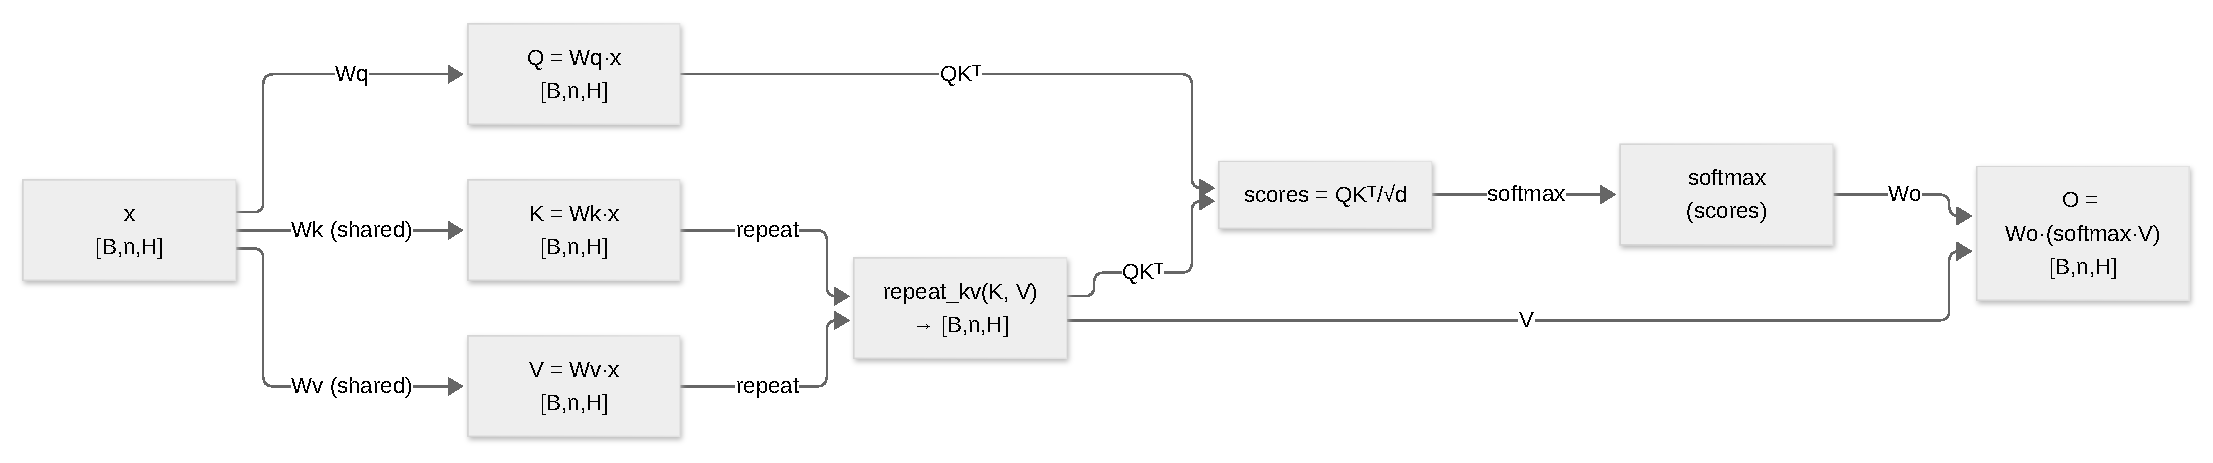
\includegraphics{../paper/figures/mixers/gqa.pdf}}
\caption{Flujo de datos de la atención por consultas agrupadas: las claves y los valores se proyectan a menos cabezas, se expanden mediante repetición entrelazada y se comparten en cada grupo de cabezas de consulta.}
\label{fig:mixer-gqa}
\end{figure}
La atención por consultas agrupadas (GQA) \citep{ainslie_gqa_2023} tiende un puente entre la atención multi-cabeza (MHA) y la atención multi-consulta (MQA) al particionar las cabezas de consulta en grupos, cada uno compartiendo una sola cabeza clave-valor. Si $h$ es el número total de cabezas de atención, $h_k$ es el número de cabezas clave-valor, y $G = h / h_k$ es el tamaño del grupo, entonces cada grupo de $G$ cabezas de consulta comparte una cabeza KV:

\begin{algorithmic}[1]
\State \textbf{Entrada:} $\mathbf{Q} \in \mathbb{R}^{n \times h \cdot d_h}$, $\mathbf{K} \in \mathbb{R}^{n \times h_k \cdot d_h}$, $\mathbf{V} \in \mathbb{R}^{n \times h_k \cdot d_h}$
\State $\mathbf{K}_{\text{completo}} \gets \texttt{repeat\_interleave}(\mathbf{K}, G)$ \Comment{expandir de $h_k$ a $h$ cabezas}
\State $\mathbf{V}_{\text{completo}} \gets \texttt{repeat\_interleave}(\mathbf{V}, G)$
\State $\text{puntajes} \gets \frac{\mathbf{Q}\mathbf{K}_{\text{completo}}^\top}{\sqrt{d_h}} \in \mathbb{R}^{n \times n}$ \Comment{producto punto estándar tras expansión}
\State $\text{pesos\_atencion} \gets \texttt{softmax}(\text{puntajes}, \text{eje}=1)$
\State \textbf{Salida:} $\mathbf{Y} = \text{pesos\_atencion} \cdot \mathbf{V}_{\text{completo}} \in \mathbb{R}^{n \times h \cdot d_h}$
\end{algorithmic}

GQA interpola suavemente entre MHA ($h_k = h$, $G = 1$) y MQA ($h_k = 1$, $G = h$). La ventaja clave es un balance ajustable entre la huella del caché KV y la capacidad representacional. Cada cabeza KV adicional consume $2 \cdot d_h \cdot n$ bytes extra en el caché, por lo que reducir $h_k$ produce ahorros proporcionales de memoria.

\begin{itemize}[leftmargin=*]
    \item \textbf{Complejidad de entrenamiento}: $\mathcal{O}(n^2 \cdot h \cdot d_h)$ (idéntico a MHA tras la expansión de cabezas).
    \item \textbf{Complejidad de inferencia}: $\mathcal{O}(n)$ por token, espacio de caché KV $\mathcal{O}(h_k \cdot n \cdot d_h)$.
    \item \textbf{Fortalezas}: Balance flexible de cabezas; probado a escala (Llama 2 y 3 usan $h_k = 8$ cabezas KV con $h = 32$ cabezas de consulta); reduce el caché KV en factor $G \times$; soporta inferencia rápida con FlashAttention.
    \item \textbf{Debilidades}: Menos cabezas KV pueden reducir la capacidad representacional en modelos pequeños; requerir que $h_k$ divida a $h$ restringe las opciones arquitectónicas.
\end{itemize}

\subsection{Arquitecturas Recurrentes y Retentivas}

\subsubsection{Redes Retentivas (RetNet)}

\begin{figure}[H]
\centering
\fitfigure{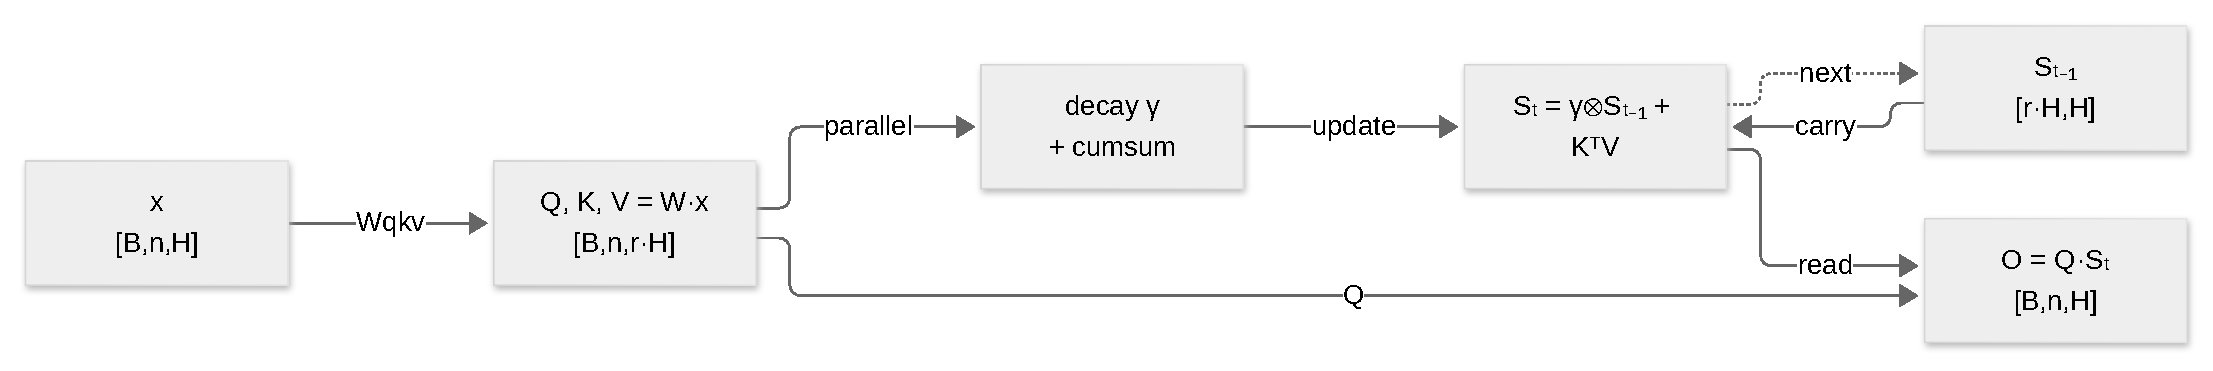
\includegraphics{../paper/figures/mixers/retnet.pdf}}
\caption{Flujo de datos de RetNet: proyecciones Q/K/V paralelas alimentan una recurrencia de estado con decaimiento; el estado se propaga entre pasos y la salida lo lee con la consulta.}
\label{fig:mixer-retnet}
\end{figure}
RetNet \citep{sun_retentive_2023} unifica tres paradigmas de cómputo: entrenamiento paralelo, inferencia recurrente y despliegue por fragmentos. Su innovación central es el \textbf{mecanismo de retención}, que utiliza una matriz de decaimiento exponencial fija para modelar la importancia temporal:

\begin{algorithmic}[1]
\State \textbf{Forma paralela (entrenamiento):}
\State $\text{matriz\_decaimiento}[i,j] \gets \gamma^{i-j}$ para $i \geq j$, si no $0$ \Comment{decaimiento exponencial causal}
\State $\text{matriz\_decaimiento}[i,j] \gets 0$ para $i < j$ \Comment{enmascaramiento causal}
\State $\mathbf{Y}_{\text{paralelo}} \gets (\mathbf{Q}\mathbf{K}^\top \odot \text{matriz\_decaimiento}) \mathbf{V}$ \Comment{multiplicación elemento a elemento con decaimiento}
\end{algorithmic}

\begin{algorithmic}[1]
\State \textbf{Forma recurrente (inferencia):}
\For{$t = 1, \ldots, n$}
    \State $\mathbf{s}_t \gets \gamma \mathbf{s}_{t-1} + \mathbf{k}_t \mathbf{v}_t^\top$ \Comment{actualización de estado con decaimiento}
    \State $\mathbf{y}_t \gets \mathbf{q}_t \mathbf{s}_t$ \Comment{salida mediante interacción consulta-estado}
\EndFor
\end{algorithmic}

El escalar de decaimiento $\gamma \in (0,1)$ controla la ventana temporal. RetNet utiliza \textbf{retención multi-escala} con diferentes valores de $\gamma$ por cabeza (ej., $\gamma = 1 - 2^{-5}, 1 - 2^{-6}, \ldots$), permitiendo dependencias a corto y largo plazo simultáneamente. El modo recurrente por fragmentos divide las secuencias en fragmentos, procesa cada fragmento en paralelo y enhebra un estado recurrente entre fragmentos.

\begin{itemize}[leftmargin=*]
    \item \textbf{Complejidad de entrenamiento}: $\mathcal{O}(n^2 \cdot d)$ (paralela), o $\mathcal{O}(n \cdot c \cdot d)$ (recurrente por fragmentos con tamaño de fragmento $c$).
    \item \textbf{Complejidad de inferencia}: $\mathcal{O}(1)$ por token, $\mathcal{O}(d^2)$ espacio de estado (matriz fija).
    \item \textbf{Fortalezas}: Inferencia en tiempo constante; triple paradigma de cómputo; consolidación multi-escala.
    \item \textbf{Debilidades}: El decaimiento fijo impone un sesgo inductivo rígido; puede truncar patrones de largo alcance aprendidos.
\end{itemize}

\subsubsection{Mamba: Modelos de Espacio de Estado Selectivos}

\begin{figure}[H]
\centering
\fitfigure{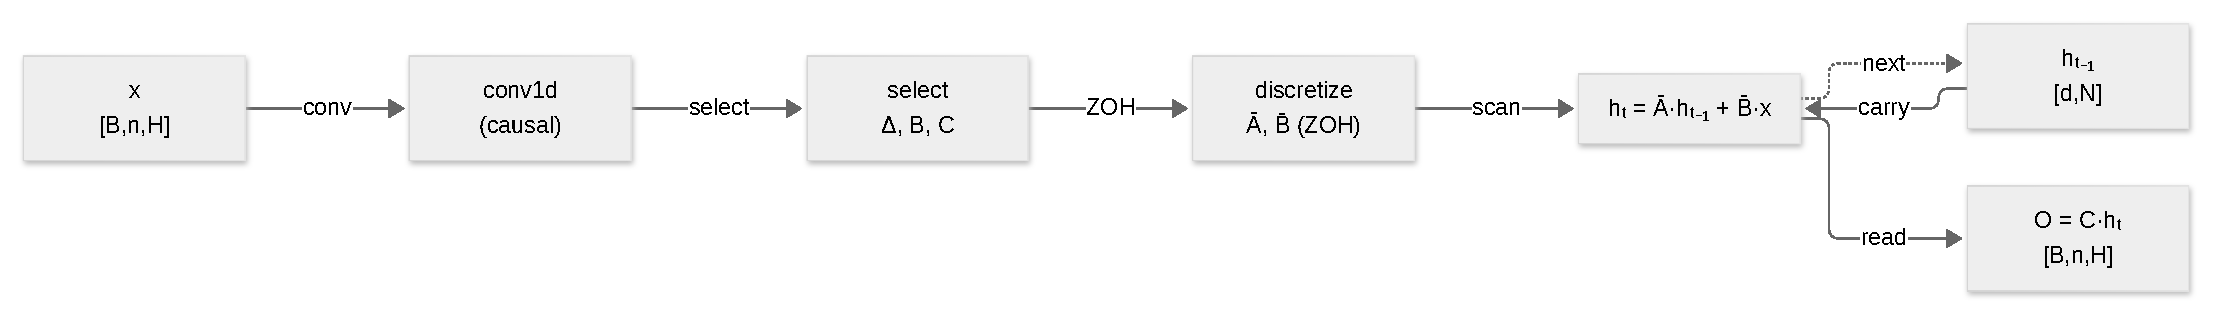
\includegraphics{../paper/figures/mixers/mamba.pdf}}
\caption{Flujo de datos de Mamba: una convolución causal alimenta selecciones de $\Delta$, $B$ y $C$ dependientes de la entrada, la discretización ZOH y un escaneo selectivo de espacio de estados cuyo estado se propaga entre pasos.}
\label{fig:mixer-mamba}
\end{figure}
Mamba \citep{gu_mamba_2023} enmarca la recurrencia como un sistema dinámico de tiempo continuo con parámetros dependientes de la entrada, logrando tanto entrenamiento lineal como inferencia en tiempo constante:

\begin{algorithmic}[1]
\State \textbf{Dinámica continua:} $h'(t) = \mathbf{A} h(t) + \mathbf{B} x(t)$, \quad $y(t) = \mathbf{C} h(t)$
\State \textbf{Discretización con tamaño de paso $\Delta_t$:}
\State $\bar{\mathbf{A}}_t \gets \exp(\Delta_t \mathbf{A})$
\State $\bar{\mathbf{B}}_t \gets (\Delta_t \mathbf{A})^{-1} (\exp(\Delta_t \mathbf{A}) - \mathbf{I}) \Delta_t \mathbf{B}_t$
\State \textbf{Actualización recurrente:}
\For{$t = 1, \ldots, n$}
    \State $\Delta_t \gets \text{softplus}(\text{Lineal}(x_t))$ \Comment{tamaño de paso dependiente de la entrada}
    \State $\mathbf{B}_t \gets \text{Lineal}(x_t)$, \quad $\mathbf{C}_t \gets \text{Lineal}(x_t)$ \Comment{matrices de proyección dependientes de la entrada}
    \State $h_t \gets \bar{\mathbf{A}}_t h_{t-1} + \bar{\mathbf{B}}_t x_t$ \Comment{transición de estado}
    \State $y_t \gets \mathbf{C}_t h_t$ \Comment{proyección de salida}
\EndFor
\end{algorithmic}

La innovación crítica es que $\mathbf{A}$ (la matriz del sistema) \textit{no} depende de la entrada, pero $\Delta_t$, $\mathbf{B}_t$ y $\mathbf{C}_t$ sí, haciendo que el sistema sea \textbf{variante en el tiempo}. Esta selectividad permite al modelo \textit{ignorar} información irrelevante estableciendo $\Delta_t$ cerca de cero, creando efectivamente una compuerta. Un algoritmo de escaneo paralelo consciente del hardware implementa la recurrencia eficientemente en GPUs fusionando el cómputo dentro de SRAM, evitando el costoso ancho de banda de HBM.

\begin{itemize}[leftmargin=*]
    \item \textbf{Complejidad de entrenamiento}: $\mathcal{O}(n \cdot d)$ mediante escaneo consciente del hardware (lineal en la longitud de la secuencia).
    \item \textbf{Complejidad de inferencia}: $\mathcal{O}(1)$ por token, $\mathcal{O}(d)$ estado (vector oculto).
    \item \textbf{Fortalezas}: Logra entrenamiento lineal e inferencia constante simultáneamente; práctico en secuencias largas (millones de tokens).
    \item \textbf{Debilidades}: La compresión del vector de estado puede debilitar la copia exacta y la recuperación asociativa densa en comparación con la atención completa.
\end{itemize}

\subsection{Transformers de Profundidad Continua: Integración EDO}

\subsubsection{Transformer EDO}

\begin{figure}[H]
\centering
\fitfigure{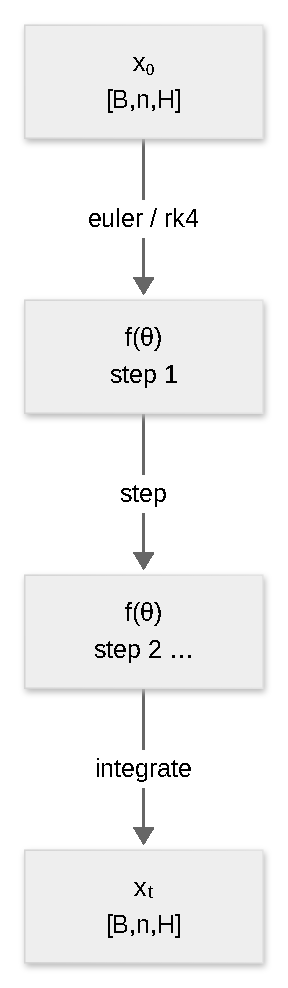
\includegraphics{../paper/figures/mixers/ode.pdf}}
\caption{Flujo de datos del bloque transformer EDO: el estado oculto se integra mediante uno o más pasos de Euler/RK4 antes de leer la salida.}
\label{fig:mixer-ode}
\end{figure}
El Transformer EDO \citep{zhang_continuous_2021} interpreta la profundidad de la red como integración numérica de un sistema dinámico continuo, utilizando solucionadores Runge-Kutta de orden superior para reducir el error de truncamiento:

\begin{algorithmic}[1]
\State \textbf{Formulación continua:} $\frac{dh(t)}{dt} = f_\theta(h(t), t)$ donde $f_\theta$ es la subred del transformer
\State \textbf{Aproximación discreta Runge-Kutta-4:}
\State $k_1 \gets f_\theta(h_t, t)$
\State $k_2 \gets f_\theta(h_t + \tfrac{1}{2}k_1, t + \tfrac{1}{2}\Delta t)$
\State $k_3 \gets f_\theta(h_t + \tfrac{1}{2}k_2, t + \tfrac{1}{2}\Delta t)$
\State $k_4 \gets f_\theta(h_t + k_3, t + \Delta t)$
\State $h_{t+1} \gets h_t + \frac{\Delta t}{6}(k_1 + 2k_2 + 2k_3 + k_4)$ \Comment{combinación ponderada}
\end{algorithmic}

En lugar de las conexiones residuales simples de Euler $h_{t+1} = h_t + f_\theta(h_t)$, el bloque RK4 calcula cuatro evaluaciones intermedias y las combina con los pesos clásicos de RK4. Para evitar gradientes que se desvanecen, la arquitectura introduce \textbf{compuertas aprendidas} que interpolan entre aproximaciones intermedias:

\begin{algorithmic}[1]
\State $g \gets \sigma(\text{Lineal}([k_1, k_2, k_3, k_4]))$ \Comment{compuerta aprendible}
\State $h_{t+1} \gets h_t + g \cdot k_1 + (1-g) \cdot k_2$ \Comment{refinamiento interpolado}
\end{algorithmic}

Esta formulación reduce el número efectivo de parámetros mediante el uso compartido de pesos---la misma $f_\theta$ se evalúa múltiples veces---proporcionando un refinamiento de trayectoria más rico.

\begin{itemize}[leftmargin=*]
    \item \textbf{Complejidad de entrenamiento}: $\mathcal{O}(k \cdot n^2 \cdot d)$ donde $k$ es el orden RK (4 para RK4).
    \item \textbf{Complejidad de inferencia}: $\mathcal{O}(k \cdot n)$ por token (mayor sobrecarga constante).
    \item \textbf{Fortalezas}: Precisión significativamente mayor en tareas de generación (BLEU de última generación); eficiente en parámetros mediante uso compartido de pesos.
    \item \textbf{Debilidades}: Alto costo de cómputo por paso; la latencia de inferencia aumenta por un factor constante $k$; requiere compuertas complejas para la estabilidad.
\end{itemize}

\subsection{Memoria en Tiempo de Prueba: Titans}

\begin{figure}[H]
\centering
\fitfigure{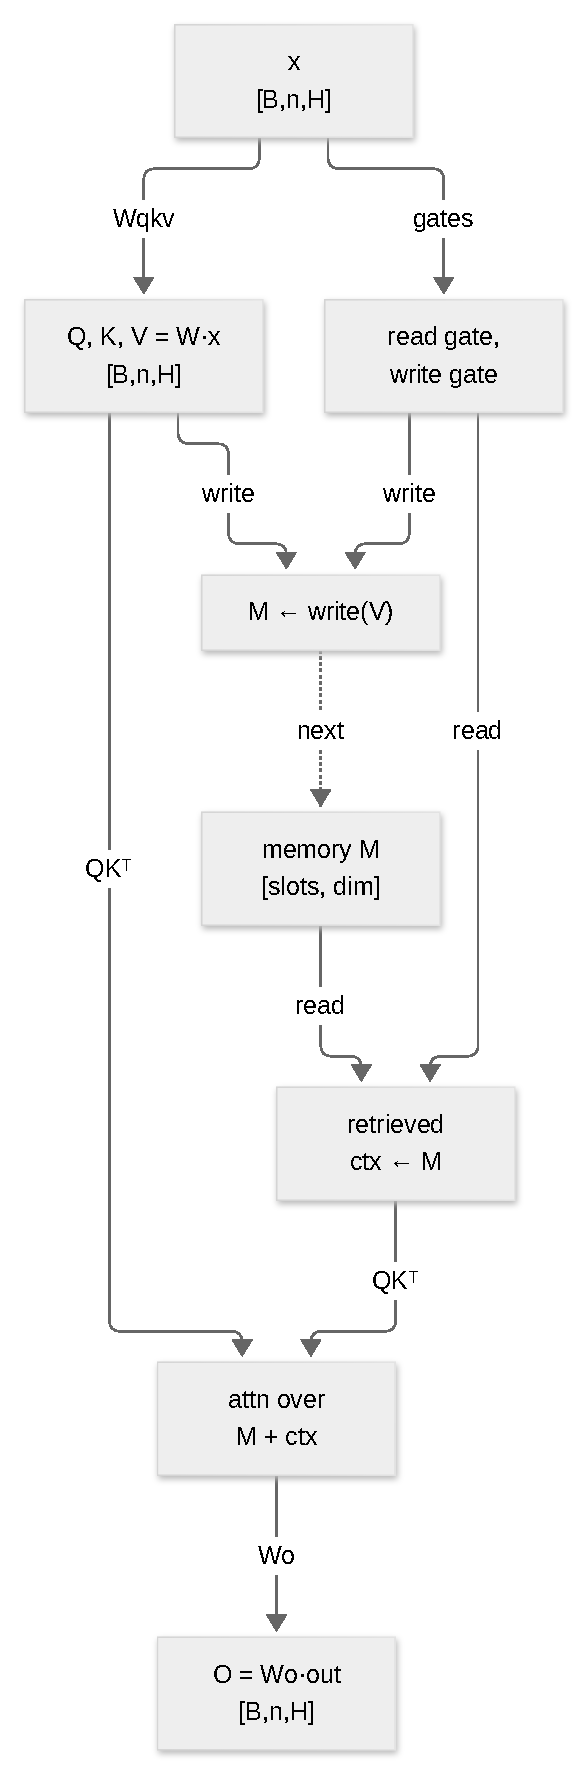
\includegraphics{../paper/figures/mixers/titan.pdf}}
\caption{Flujo de datos de la memoria en tiempo de prueba de Titans: la atención densa Q/K/V opera sobre una ventana local mientras compuertas de lectura y escritura actualizan una memoria asociativa que se propaga entre pasos.}
\label{fig:mixer-titan}
\end{figure}

La arquitectura Titans \citep{behrouz_titans_2025} introduce una dimensión ortogonal: en lugar de pesos estáticos, el modelo mantiene una memoria aprendible que se \textit{actualiza durante la inferencia} basada en una señal impulsada por sorpresa:

\begin{algorithmic}[1]
\State \textbf{Atención local a corto plazo:} Aplicar atención estándar o dispersa dentro de una ventana de contexto fija $c$
\State $y_t^{\text{local}} \gets \text{Atencion}(q_t, k_{[t-c:t]}, v_{[t-c:t]})$
\State \textbf{Señal de actualización de memoria (sorpresa):}
\State $S_t \gets \eta_t S_{t-1} - \theta_t \nabla_\ell(\mathcal{M}_{t-1}; x_t)$ \Comment{sorpresa como gradiente de la pérdida respecto a la memoria}
\State $\mathcal{M}_t \gets (1 - \alpha_t) \mathcal{M}_{t-1} + S_t$ \Comment{memoria actualizada mediante EMA}
\State \textbf{Recuperación de memoria a largo plazo:}
\State $y_t^{\text{memoria}} \gets \mathcal{M}_t^* (q_t)$ \Comment{consultar módulo de memoria para información recuperada}
\State \textbf{Combinación de salida:}
\State $y_t \gets y_t^{\text{local}} + \text{compuerta}(y_t^{\text{memoria}})$ \Comment{combinar memoria local y recuperada}
\end{algorithmic}

El módulo de memoria $\mathcal{M}$ se actualiza literalmente durante el paso hacia adelante calculando gradientes de una pérdida asociativa y aplicando pasos de SGD con momento. Las tasas de decaimiento $\eta_t, \theta_t, \alpha_t$ son en sí mismas dependientes de la entrada, permitiendo al modelo cambiar de paradigma de memoria cuando el contexto cambia.

\begin{itemize}[leftmargin=*]
    \item \textbf{Complejidad de entrenamiento}: Aproximadamente $\mathcal{O}(c^2 + n \cdot f)$ donde $c$ es la ventana local y $f$ es la sobrecarga de actualización de memoria.
    \item \textbf{Complejidad de inferencia}: $\mathcal{O}(c^2)$ atención local más $\mathcal{O}(1)$ recuperación de memoria por token.
    \item \textbf{Fortalezas}: Maneja longitudes de contexto extremas; permite recuperación asociativa real; la memoria se adapta a la entrada.
    \item \textbf{Debilidades}: Significativamente más complejo; la inferencia incluye cálculos de gradientes; mayor sobrecarga de coordinación.
\end{itemize}

\subsection{Despacho de Mezclador Guiado por Patrón}

El código base selecciona un mezclador por bloque a partir del \texttt{layer\_pattern} configurado. La lógica de despacho enruta los bloques dispersos en tiempo de inferencia (\texttt{fasa\_attn}, \texttt{sparge\_attn}) a atención estándar densa mientras el modelo está en modo entrenamiento, y a su implementación dispersa durante la evaluación; el resto de bloques se enruta a la implementación de familia correspondiente.

\begin{algorithm}[t]
\caption{Paso Adelante del Mezclador Guiado por Patrón (Conceptual)}
\begin{algorithmic}[1]
\Require Estados ocultos $H$, patrón $P$, índice de capa $\ell$
\State $m \gets P[\ell \bmod |P|]$
\If{$m \in \{\texttt{fasa\_attn}, \texttt{sparge\_attn}\}$ y el modelo está en modo entrenamiento}
    \State $H \gets \text{softmax-attention}(H)$ \Comment{atención densa sustituta, mismas proyecciones}
\ElsIf{$m=\texttt{standard\_attn}$}
    \State $H \gets \text{softmax-attention}(H)$
\ElsIf{$m=\texttt{sigmoid\_attn}$}
    \State $H \gets \text{sigmoid-attention}(H)$
\ElsIf{$m\in\{\texttt{retnet},\texttt{retnet\_attn}\}$}
    \State $H \gets \text{retention}(H)$
\ElsIf{$m=\texttt{mamba}$}
    \State $H \gets \text{selective-ssm}(H)$
\ElsIf{$m=\texttt{ode}$}
    \State $H \gets \text{rk-step}(H)$
\ElsIf{$m$ es una clave de atención dispersa}
    \State $H \gets \text{sparse-attention-family}(H)$
\ElsIf{$m$ es una clave de atención con compuerta}
    \State $H \gets \text{gated-attention-family}(H)$
\Else
    \State $H \gets \text{memory-augmented-attn}(H)$
\EndIf
\State \Return $H$
\end{algorithmic}
\end{algorithm}

El campo exhibe una progresión clara a lo largo de dos ejes: (i) \textbf{eficiencia computacional}, pasando de $O(n^2)$ a $O(n)$ u $O(1)$, y (ii) \textbf{adaptabilidad de memoria}, pasando de pesos estáticos a modelos dinámicos actualizados en tiempo de prueba. La atención estándar sigue siendo la línea base de expresividad; Mamba y RetNet representan la frontera práctica de eficiencia; Titans introduce un eje de innovación ortogonal (aprendizaje en tiempo de prueba). La elección de arquitectura refleja la restricción fundamental de ingeniería: expresividad versus costo de despliegue. La familia de atención latente, que comprime el caché KV en un latente de rango bajo, se cubre en el Apéndice~\ref{sec:annex-latent}.
\section{Familias de Atención Latente y de Rango Bajo}
\label{sec:annex-latent}

Este anexo cubre la familia de mecanismos de atención de compresión latente / de rango bajo de KV. Estas arquitecturas comprimen el estado clave--valor por token en un vector latente de rango bajo que es la única cantidad materializada en el caché KV durante la decodificación, luego reconstruyen las claves y valores completos de todas las cabezas al vuelo. La familia unifica diseños de consulta agrupada, latente, factorizado y latente temporal bajo un cuello de botella de rango bajo común.

\subsection{Atención Latente Multi-Cabeza (MLA)}

\begin{figure}[H]
\centering
\fitfigure{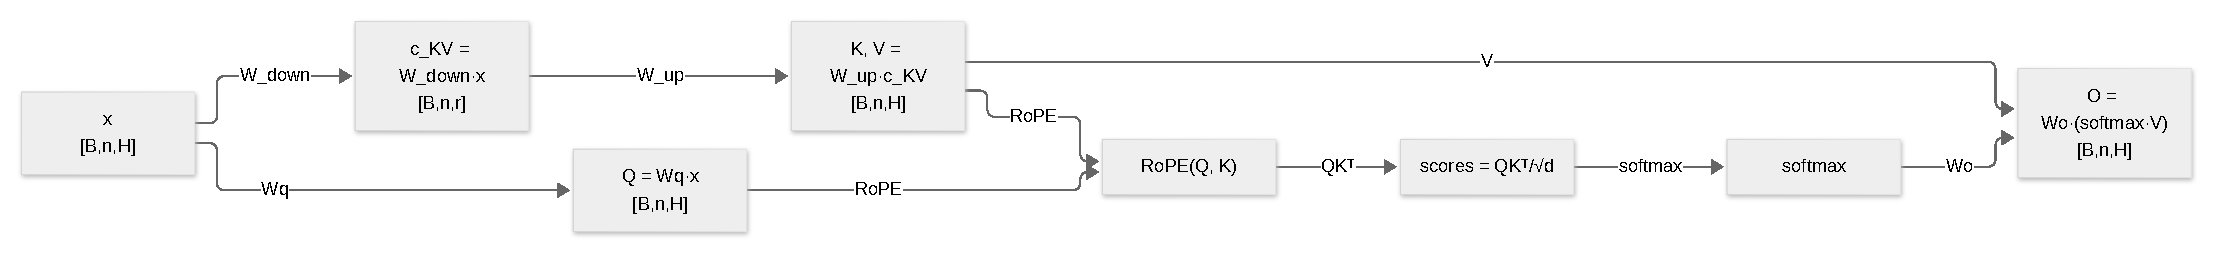
\includegraphics{../paper/figures/mixers/mla.pdf}}
\caption{Flujo de datos de la atención latente multi-cabeza: las claves y los valores se proyectan hacia abajo a un latente de rango bajo, se proyectan de vuelta y se atienden con la consulta tras RoPE.}
\label{fig:mixer-mla}
\end{figure}
La Atención Latente Multi-Cabeza (MLA, por sus siglas en inglés) \citep{mehta_mla_2025} comprime el estado clave--valor por token en un único vector latente de rango bajo $c_{KV}$ de rango $r_{kv}$, el cual es la única cantidad materializada en el caché KV durante la decodificación. Un par de matrices de up-proyección reconstruye las claves y valores completos de todas las cabezas al vuelo, mientras que RoPE se aplica a los tensores de consulta y clave descomprimidos para preservar la estructura posicional. Los autores muestran que el ancho latente óptimo de Pareto se sitúa cerca de $r_{kv} = d_{\text{oculto}} / 2$, punto en el cual MLA reduce a la mitad el caché KV pero iguala la calidad de la atención multi-cabeza (MHA) en modelos pequeños.

\subsubsection{Formulación Matemática}
\[
c_{KV} = W_{DKV}\, x \in \mathbb{R}^{r_{kv}}, \qquad
k = W_{UK}\, c_{KV}, \qquad
v = W_{UV}\, c_{KV}, \qquad
q = W_{Q}\, x.
\]
\[
\tilde q = \text{RoPE}(q), \quad \tilde k = \text{RoPE}(k), \qquad
\text{atencion} = \texttt{softmax}\!\left(\frac{\tilde q\, \tilde k^\top}{\sqrt{d_h}}\right) v.
\]

\subsubsection{Pseudocódigo Algorítmico}
\begin{algorithmic}[1]
\State \textbf{Entrada:} estado oculto $x \in \mathbb{R}^{n \times d}$, rango $r_{kv}$, proyecciones $W_{DKV}, W_{UK}, W_{UV}, W_{Q}$
\State $c_{KV} \gets W_{DKV}\, x$ \Comment{down-proyección a latente de rango $r_{kv}$ (en caché en inferencia)}
\State $k \gets W_{UK}\, c_{KV}$, \quad $v \gets W_{UV}\, c_{KV}$ \Comment{up-proyección a cabezas completas}
\State $q \gets W_{Q}\, x$
\State $\tilde q \gets \text{RoPE}(q)$, \quad $\tilde k \gets \text{RoPE}(k)$ \Comment{aplicar embeddings rotatorios}
\State $\text{pesos} \gets \texttt{softmax}(\tilde q\, \tilde k^\top / \sqrt{d_h})$
\State \textbf{Salida:} $\mathbf{Y} = \text{pesos} \cdot v$
\end{algorithmic}

\subsubsection{Características Clave}
\begin{itemize}[leftmargin=*]
    \item \textbf{Complejidad de entrenamiento}: $\mathcal{O}(n^2 \cdot d)$ (atención completa sobre cabezas descomprimidas).
    \item \textbf{Complejidad de inferencia}: $\mathcal{O}(n)$ por token, espacio de caché KV $\mathcal{O}(r_{kv} \cdot n)$ (sólo latente).
    \item \textbf{Entrenable}: totalmente entrenable; $r_{kv}$ es un hiperparámetro (óptimo de Pareto $\approx d/2$).
    \item \textbf{Fortalezas}: reduce a la mitad el caché KV frente a MHA con calidad equivalente; compatible con RoPE; cuello de botella latente limpio.
    \item \textbf{Limitaciones}: la up-proyección añade FLOPs de decodificación; el rango latente es un presupuesto global fijo compartido entre cabezas.
\end{itemize}

\subsection{Atención Latente por Consultas Agrupadas (GQLA)}

\begin{figure}[H]
\centering
\fitfigure{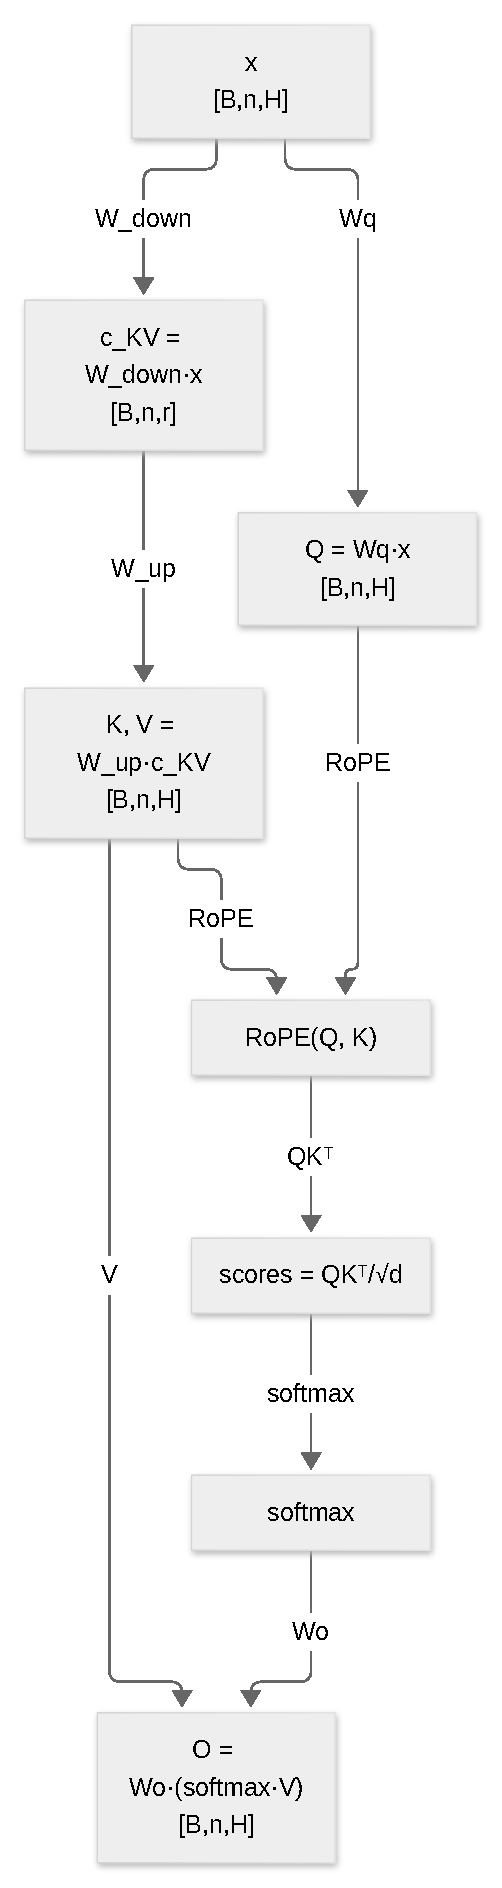
\includegraphics{../paper/figures/mixers/gqla.pdf}}
\caption{Flujo de datos de la atención latente por consultas agrupadas: la caché latente compartida se proyecta hacia arriba a cabezas de clave/valor y se combina con consultas agrupadas.}
\label{fig:mixer-gqla}
\end{figure}
La Atención Latente por Consultas Agrupadas (GQLA, por sus siglas en inglés) \citep{meng_gqla_2026} es una modificación mínima de MLA que expone dos rutas de decodificación algebraicamente equivalentes sobre los mismos pesos entrenados: una ruta MQA-absorb (que fusiona la up-proyección en la consulta, óptima en hardware tipo H100) y una ruta GQA-expanded (que materializa claves/valores completos, óptima en hardware H20 / predicción multi-token). Las dos rutas son matemáticamente idénticas porque la up-proyección es lineal, de modo que $\texttt{softmax}(q_{\text{absorbido}} \cdot c_{KV}^\top) = \texttt{softmax}((q \cdot W_{UK}^\top) \cdot c_{KV}^\top)$, permitiendo un despacho adaptativo al hardware sin reentrenamiento.

\subsubsection{Formulación Matemática}
Mismo latente que MLA:
\[
c_{KV} = W_{DKV}\, x, \qquad k = W_{UK}\, c_{KV}, \qquad v = W_{UV}\, c_{KV}, \qquad q = W_{Q}\, x.
\]
\[
\text{Ruta A (MQA-absorb): } \text{atencion} = \texttt{softmax}\!\left(\frac{(q\, W_{UK}^\top)\, c_{KV}^\top}{\sqrt{d_h}}\right) (W_{UV}\, c_{KV}).
\]
\[
\text{Ruta B (GQA-expanded): } \text{atencion} = \texttt{softmax}\!\left(\frac{q\, k^\top}{\sqrt{d_h}}\right) v, \quad k = W_{UK} c_{KV},\ v = W_{UV} c_{KV}.
\]

\subsubsection{Pseudocódigo Algorítmico}
\begin{algorithmic}[1]
\State \textbf{Entrada:} $x$, pesos $W_{DKV}, W_{UK}, W_{UV}, W_{Q}$, bandera de hardware $\text{hw} \in \{\text{H100}, \text{H20}\}$
\State $c_{KV} \gets W_{DKV}\, x$ \Comment{latente compartido, en caché}
\State $q \gets W_{Q}\, x$
\If{$\text{hw} == \text{H100}$} \Comment{ruta MQA-absorb}
    \State $q_{\text{abs}} \gets q\, W_{UK}^\top$ \Comment{absorber up-proyección en la consulta}
    \State $\text{pesos} \gets \texttt{softmax}(q_{\text{abs}}\, c_{KV}^\top / \sqrt{d_h})$
    \State $\mathbf{Y} \gets \text{pesos} \cdot (W_{UV}\, c_{KV})$
\Else \Comment{ruta GQA-expanded}
    \State $k \gets W_{UK}\, c_{KV}$, \quad $v \gets W_{UV}\, c_{KV}$
    \State $\text{pesos} \gets \texttt{softmax}(q\, k^\top / \sqrt{d_h})$
    \State $\mathbf{Y} \gets \text{pesos} \cdot v$
\EndIf
\State \textbf{Salida:} $\mathbf{Y}$
\end{algorithmic}

\subsubsection{Características Clave}
\begin{itemize}[leftmargin=*]
    \item \textbf{Complejidad de entrenamiento}: $\mathcal{O}(n^2 \cdot d)$, idéntica a MLA.
    \item \textbf{Complejidad de inferencia}: $\mathcal{O}(n)$ por token, estado latente $\mathcal{O}(r_{kv} \cdot n)$; ruta elegida por hardware.
    \item \textbf{Entrenable}: se entrena una sola vez; las dos rutas de decodificación reutilizan los mismos pesos.
    \item \textbf{Fortalezas}: decodificación adaptativa al hardware sin pérdida de calidad; la equivalencia algebraica garantiza consistencia.
    \item \textbf{Limitaciones}: mismas compensaciones de rango latente que MLA; la selección de ruta es una heurística de despliegue.
\end{itemize}

\subsection{Atención Multi-Cabeza de Rango Bajo (MLRA)}

\begin{figure}[H]
\centering
\fitfigure{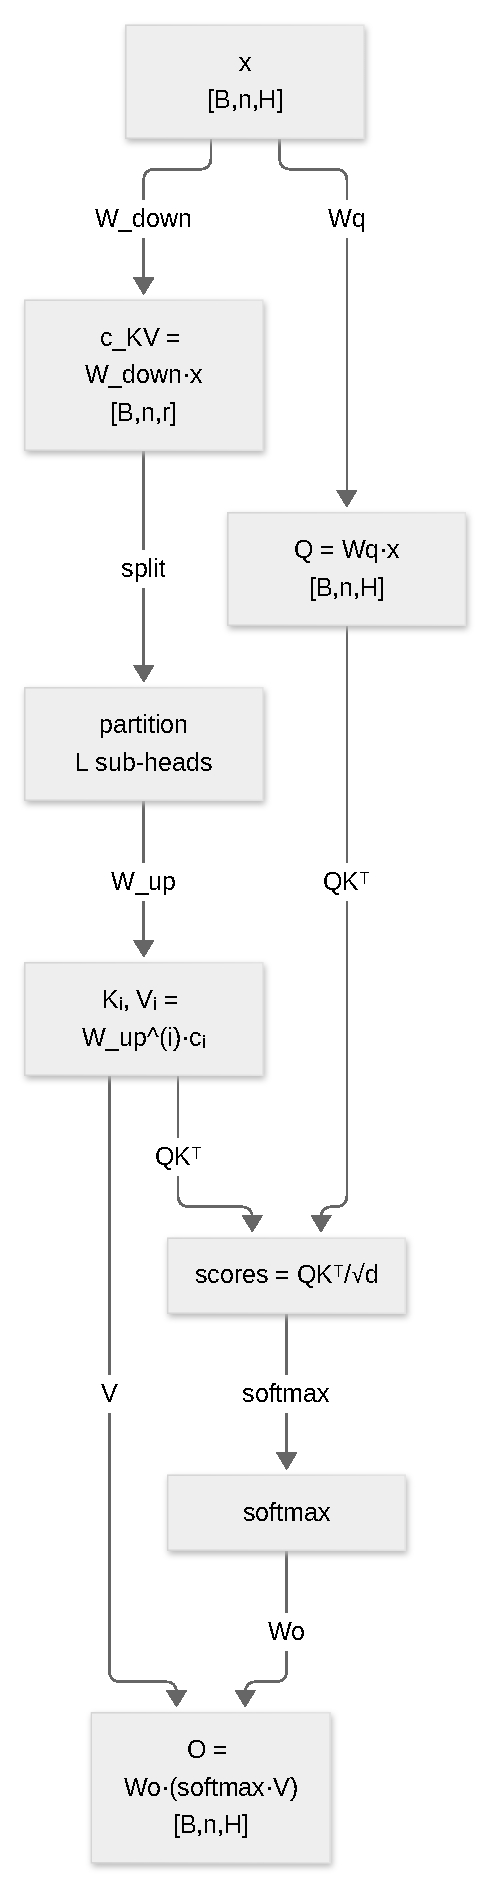
\includegraphics{../paper/figures/mixers/mlra.pdf}}
\caption{Flujo de datos de la atención multi-cabeza de rango bajo: el latente se particiona entre sub-cabezas, cada una con su propia proyección ascendente, antes de la atención.}
\label{fig:mixer-mlra}
\end{figure}
La Atención Multi-Cabeza de Rango Bajo (MLRA, por sus siglas en inglés) \citep{liu_mlra_2026} refactoriza el latente único de MLA en $L$ sub-cabezas disjuntas cada una de rango $r/L$, de modo que el caché KV puede particionarse entre $L$ dispositivos para una decodificación tensor-paralela de 4 vías (cada dispositivo carga sólo $1/L$ del caché). Las up-proyecciones por sub-cabeza reconstruyen la porción correspondiente de las cabezas completas y se concatenan, logrando una aceleración de decodificación de 2.8$\times$ sobre MLA preservando el presupuesto latente global.

\subsubsection{Formulación Matemática}
\[
c_{KV} = [c_1, c_2, \ldots, c_L], \quad c_i \in \mathbb{R}^{r/L}, \qquad c_{KV} = W_{DKV}\, x.
\]
\[
k_i = W_{UK}^{(i)}\, c_i, \quad v_i = W_{UV}^{(i)}\, c_i, \qquad
k = [k_1; \ldots; k_L], \quad v = [v_1; \ldots; v_L].
\]
\[
\text{atencion} = \texttt{softmax}\!\left(\frac{q\, k^\top}{\sqrt{d_h}}\right) v.
\]

\subsubsection{Pseudocódigo Algorítmico}
\begin{algorithmic}[1]
\State \textbf{Entrada:} $x$, número de sub-cabezas $L$, proyecciones por sub-cabeza $W_{UK}^{(i)}, W_{UV}^{(i)}$
\State $c_{KV} \gets W_{DKV}\, x = [c_1, \ldots, c_L]$ \Comment{particionar latente en $L$ bloques}
\For{$i = 1, \ldots, L$ (en paralelo entre $L$ dispositivos)}
    \State $k_i \gets W_{UK}^{(i)}\, c_i$, \quad $v_i \gets W_{UV}^{(i)}\, c_i$
\EndFor
\State $k \gets \texttt{concat}(k_1, \ldots, k_L)$, \quad $v \gets \texttt{concat}(v_1, \ldots, v_L)$
\State $\text{pesos} \gets \texttt{softmax}(q\, k^\top / \sqrt{d_h})$
\State \textbf{Salida:} $\mathbf{Y} = \text{pesos} \cdot v$
\end{algorithmic}

\subsubsection{Características Clave}
\begin{itemize}[leftmargin=*]
    \item \textbf{Complejidad de entrenamiento}: $\mathcal{O}(n^2 \cdot d)$ (atención completa sobre cabezas concatenadas).
    \item \textbf{Complejidad de inferencia}: $\mathcal{O}(n)$ por token, estado $\mathcal{O}(r_{kv} \cdot n)$ particionado entre $L$ dispositivos.
    \item \textbf{Entrenable}: totalmente entrenable; $L$ controla la granularidad de partición.
    \item \textbf{Fortalezas}: aceleración de decodificación de 2.8$\times$; particionamiento limpio tensor-paralelo de 4 vías del caché; preserva el presupuesto latente total.
    \item \textbf{Limitaciones}: requiere que $L$ divida a $r_{kv}$; más matrices de proyección que MLA; all-reduce inter-dispositivo en la salida.
\end{itemize}

\subsection{Atención Tucker}

\begin{figure}[H]
\centering
\fitfigure{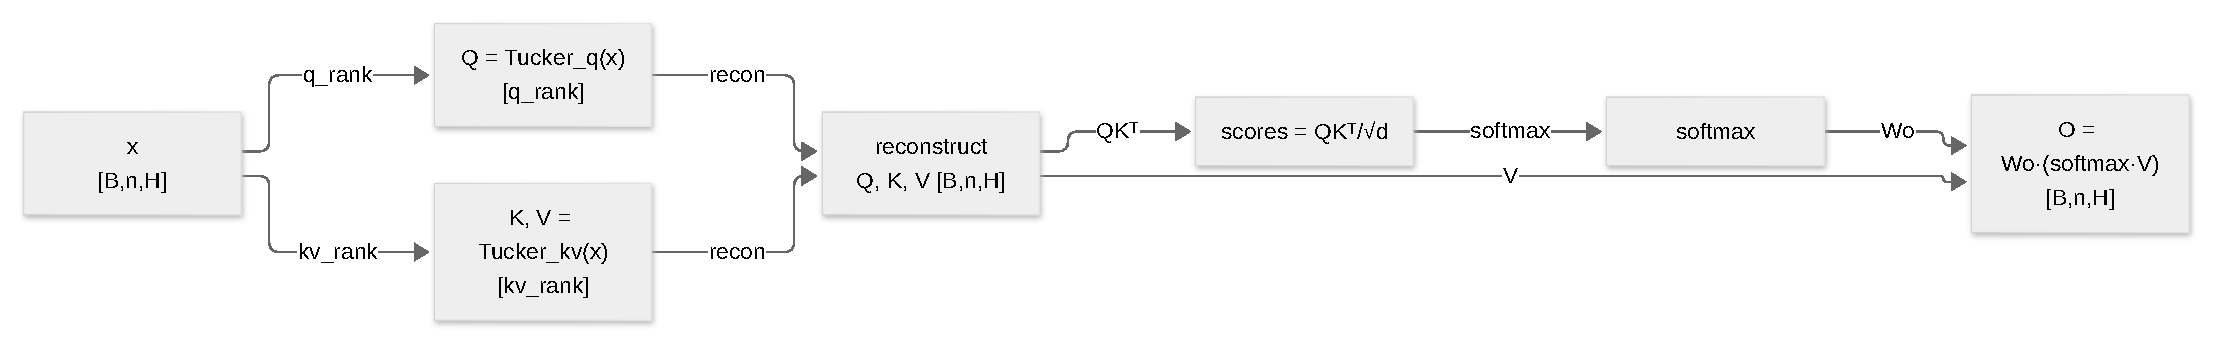
\includegraphics{../paper/figures/mixers/tucker.pdf}}
\caption{Flujo de datos de la atención Tucker: las consultas y las claves/valores se proyectan mediante factores de Tucker y se reconstruyen antes del producto escalar escalado.}
\label{fig:mixer-tucker}
\end{figure}
La Atención Tucker \citep{klein_tucker_2026} unifica MHA, GQA y MLA bajo una única factorización estilo Tucker de los tensores de pesos de consulta/clave/valor con rangos independientes $q_{\text{rank}}, k_{\text{rank}}, v_{\text{rank}}$. Se recupera MHA cuando todos los rangos igualan el tamaño oculto, GQA cuando $k_{\text{rank}} = v_{\text{rank}} < d$, y MLA cuando $k_{\text{rank}} = v_{\text{rank}}$ es igual al rango latente. Como la factorización es una repas lineal de pesos, el método es totalmente compatible con FlashAttention y RoPE, y produce un orden de magnitud menos parámetros para métricas comparables.

\subsubsection{Formulación Matemática}
\[
\mathbf{Q} = W_{Q,\text{core}}\, W_{Q,\text{factor}}\, x, \qquad
\mathbf{K} = W_{K,\text{core}}\, W_{K,\text{factor}}\, x, \qquad
\mathbf{V} = W_{V,\text{core}}\, W_{V,\text{factor}}\, x.
\]
\[
\text{atencion} = \texttt{softmax}\!\left(\frac{\mathbf{Q}\, \mathbf{K}^\top}{\sqrt{d_h}}\right) \mathbf{V}.
\]
Casos especiales: MHA $\Leftrightarrow q_{\text{rank}} = k_{\text{rank}} = v_{\text{rank}} = d$; GQA $\Leftrightarrow k_{\text{rank}} = v_{\text{rank}} < d$; MLA $\Leftrightarrow k_{\text{rank}} = v_{\text{rank}} = r_{kv}$.

\subsubsection{Pseudocódigo Algorítmico}
\begin{algorithmic}[1]
\State \textbf{Entrada:} $x$, rangos $q_{\text{rank}}, k_{\text{rank}}, v_{\text{rank}}$, matrices core/factor
\State $\mathbf{Q} \gets W_{Q,\text{core}}\, W_{Q,\text{factor}}\, x$ \Comment{consulta factorizada de rango $q_{\text{rank}}$}
\State $\mathbf{K} \gets W_{K,\text{core}}\, W_{K,\text{factor}}\, x$ \Comment{clave factorizada de rango $k_{\text{rank}}$}
\State $\mathbf{V} \gets W_{V,\text{core}}\, W_{V,\text{factor}}\, x$ \Comment{valor factorizado de rango $v_{\text{rank}}$}
\State \textbf{Aplicar RoPE a $\mathbf{Q}, \mathbf{K}$ si se usa codificación posicional}
\State $\text{pesos} \gets \texttt{softmax}(\mathbf{Q}\, \mathbf{K}^\top / \sqrt{d_h})$ \Comment{compatible con FlashAttention}
\State \textbf{Salida:} $\mathbf{Y} = \text{pesos} \cdot \mathbf{V}$
\end{algorithmic}

\subsubsection{Características Clave}
\begin{itemize}[leftmargin=*]
    \item \textbf{Complejidad de entrenamiento}: $\mathcal{O}(n^2 \cdot d)$ sobre los tensores reconstruidos.
    \item \textbf{Complejidad de inferencia}: $\mathcal{O}(n)$ por token; tamaño de caché gobernado por $k_{\text{rank}}$.
    \item \textbf{Entrenable}: los rangos son hiperparámetros; la factorización es una repas de pesos directa.
    \item \textbf{Fortalezas}: unifica MHA/GQA/MLA; reducción de parámetros de un orden de magnitud con métricas equivalentes; compatible con FlashAttention/RoPE.
    \item \textbf{Limitaciones}: dos matmuls por proyección añaden latencia; la selección de rango es un problema de ajuste por tarea.
\end{itemize}

\subsection{Atención de Cabezas Entrelazadas (IHA)}

\begin{figure}[H]
\centering
\fitfigure{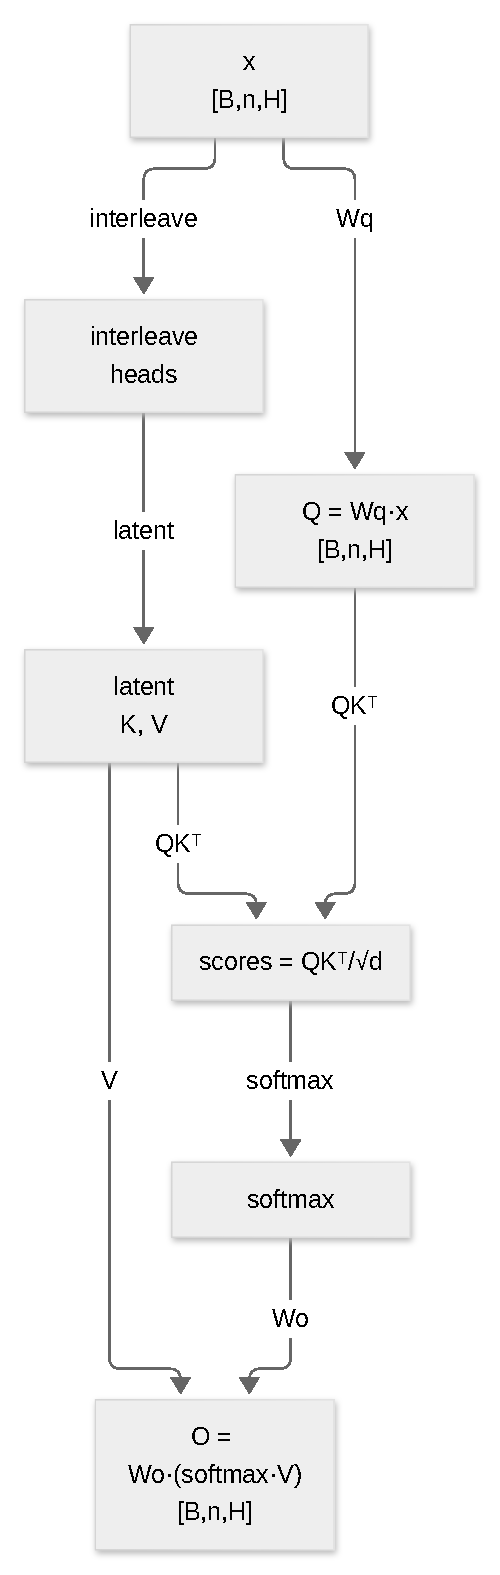
\includegraphics{../paper/figures/mixers/iha.pdf}}
\caption{Flujo de datos de la atención de cabezas entrelazadas: las cabezas se entrelazan en una representación latente de clave/valor que la consulta atiende.}
\label{fig:mixer-iha}
\end{figure}
La Atención de Cabezas Entrelazadas (IHA, por sus siglas en inglés) \citep{duvvuri_iha_2026} construye $P$ pseudo-cabezas por cabeza original (típicamente $P = H$) donde cada consulta/clave/valor pseudo es una combinación lineal aprendida de todas las $H$ cabezas originales. Esto induce hasta $P^2$ patrones de atención distintos por cabeza con una sobrecarga de $\mathcal{O}(H^2 P)$. Teóricamente, IHA necesita sólo $\Theta(\sqrt{k}\, n^2)$ parámetros frente a $\Theta(k\, n^2)$ de MHA en la tarea Polinomial; empíricamente entrega $+10$--$20\%$ en RULER de recuperación multi-clave, $+5.8\%$ en GSM8K y $+2.8\%$ en MATH-500.

\subsubsection{Formulación Matemática}
{\small
\[
q_{\text{pseudo}}[p] = \sum_{h=1}^{H} \text{mix}_q[p, h]\, q[h], \quad
k_{\text{pseudo}}[p] = \sum_{h} \text{mix}_k[p, h]\, k[h], \quad
v_{\text{pseudo}}[p] = \sum_{h} \text{mix}_v[p, h]\, v[h].
\]
}
\[
\text{atencion}_p = \texttt{softmax}\!\left(\frac{q_{\text{pseudo}}[p]\, k_{\text{pseudo}}[p]^\top}{\sqrt{d_h}}\right) v_{\text{pseudo}}[p],
\qquad
\mathbf{Y}[h] = \frac{1}{P} \sum_{p} \text{atencion}_p[h].
\]

\subsubsection{Pseudocódigo Algorítmico}
\begin{algorithmic}[1]
\State \textbf{Entrada:} por cabeza $q[h], k[h], v[h]$, matrices de mezcla $\text{mix}_q, \text{mix}_k, \text{mix}_v \in \mathbb{R}^{P \times H}$
\For{$p = 1, \ldots, P$}
    \State $q_p \gets \sum_h \text{mix}_q[p,h]\, q[h]$ \Comment{mezcla aprendida entre cabezas}
    \State $k_p \gets \sum_h \text{mix}_k[p,h]\, k[h]$, \quad $v_p \gets \sum_h \text{mix}_v[p,h]\, v[h]$
    \State $\text{atencion}_p \gets \texttt{softmax}(q_p\, k_p^\top / \sqrt{d_h})\, v_p$
\EndFor
\State \textbf{Salida:} $\mathbf{Y}[h] \gets \frac{1}{P} \sum_p \text{atencion}_p[h]$ \Comment{promediar salidas pseudo-cabeza por cabeza}
\end{algorithmic}

\subsubsection{Características Clave}
\begin{itemize}[leftmargin=*]
    \item \textbf{Complejidad de entrenamiento}: $\mathcal{O}(n^2 \cdot H \cdot P)$ con $P \approx H$, es decir $\mathcal{O}(n^2 \cdot H^2)$.
    \item \textbf{Complejidad de inferencia}: $\mathcal{O}(n)$ por token con caché KV; sobrecarga extra de mezcla $\mathcal{O}(H^2 P)$.
    \item \textbf{Entrenable}: las matrices de mezcla se aprenden; $P$ es un hiperparámetro.
    \item \textbf{Fortalezas}: eficiencia de parámetros $\Theta(\sqrt{k})$ en Polinomial; grandes ganancias en recuperación y razonamiento.
    \item \textbf{Limitaciones}: costo de mezcla cuadrático en cabezas; más patrones de atención a computar; latencia añadida con $H$ grande.
\end{itemize}

\subsection{Atención laTenT por Cabezas Agrupadas (GTA)}

\begin{figure}[H]
\centering
\fitfigure{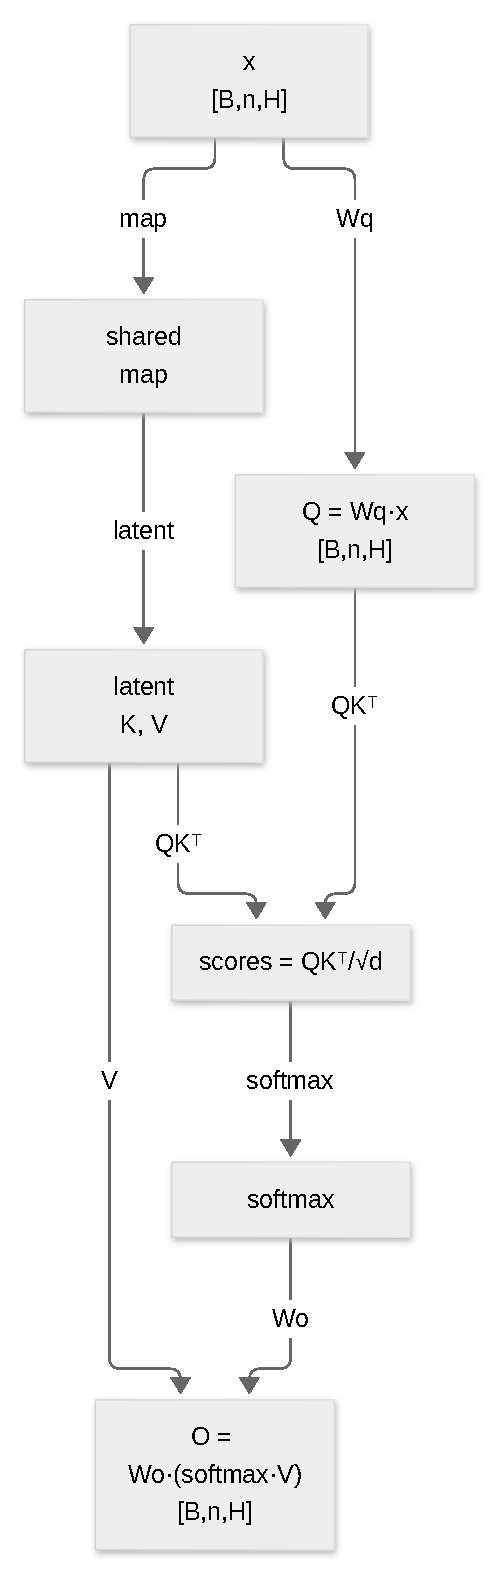
\includegraphics{../paper/figures/mixers/gta.pdf}}
\caption{Flujo de datos de la atención latente por cabezas agrupadas: un mapa compartido produce el estado latente de clave/valor que consumen las cabezas agrupadas.}
\label{fig:mixer-gta}
\end{figure}
La Atención laTenT por Cabezas Agrupadas (GTA, por sus siglas en inglés) \citep{sun_gta_2025} combina dos compresiones: (1) un \emph{mapa de atención compartido} --- un tensor de puntajes de atención por grupo de cabezas, reutilizado entre todas las cabezas del grupo, reduciendo el caché de claves; y (2) un \emph{decodificador de valores no lineal} --- el caché de valores se comprime a un latente mediante una down-proyección y se reconstruye por una up-proyección con compuerta SiLU antes de la proyección de salida. GTA reduce los FLOPs de atención hasta 62.5\% frente a GQA, encoge el caché KV hasta 70\%, y produce una aceleración de inferencia de 2$\times$ de extremo a extremo.

\subsubsection{Formulación Matemática}
{\footnotesize
\[
q_g = \texttt{mean}(q[\text{grupo } g]), \quad k_g = \texttt{mean}(k[\text{grupo } g]), \quad
\text{atencion}_g = \texttt{softmax}\!\left(\frac{q_g\, k_g^\top}{\sqrt{d_h}}\right) \text{ (reutilizado en el grupo)}.
\]
}
\[
v_{\text{latente}} = W_{DV}\, x, \qquad v = \text{SiLU}(W_{UV}\, v_{\text{latente}}), \qquad
\mathbf{Y} = \text{atencion}_g \cdot v.
\]

\subsubsection{Pseudocódigo Algorítmico}
\begin{algorithmic}[1]
\State \textbf{Entrada:} $q, k$ por cabeza, oculto $x$, partición de grupos $\{g\}$
\State $v_{\text{latente}} \gets W_{DV}\, x$ \Comment{comprimir valores a latente (en caché)}
\State $v \gets \text{SiLU}(W_{UV}\, v_{\text{latente}})$ \Comment{decodificación no lineal de valores}
\For{cada grupo $g$}
    \State $q_g \gets \texttt{mean}(q[g])$, \quad $k_g \gets \texttt{mean}(k[g])$ \Comment{consultas/claves compartidas por grupo}
    \State $\text{atencion}_g \gets \texttt{softmax}(q_g\, k_g^\top / \sqrt{d_h})$
    \State $\mathbf{Y}[g] \gets \text{atencion}_g \cdot v[g]$ \Comment{un mapa reutilizado para todas las cabezas en $g$}
\EndFor
\State \textbf{Salida:} $\mathbf{Y}$
\end{algorithmic}

\subsubsection{Características Clave}
\begin{itemize}[leftmargin=*]
    \item \textbf{Complejidad de entrenamiento}: $\mathcal{O}(n^2 \cdot G \cdot d_h)$ donde $G$ es el número de grupos (frente a $H$ cabezas en GQA).
    \item \textbf{Complejidad de inferencia}: $\mathcal{O}(n)$ por token; caché de valores $\mathcal{O}(r_v \cdot n)$, caché de claves reducido por compartición de grupo.
    \item \textbf{Entrenable}: la asignación de grupo y el rango latente son entrenables/hiperparámetros.
    \item \textbf{Fortalezas}: hasta 62.5\% de reducción de FLOPs de atención, 70\% de encogimiento de caché KV, 2$\times$ de aceleración de extremo a extremo.
    \item \textbf{Limitaciones}: el mapa compartido reduce la diversidad por cabeza; el decodificador no lineal añade latencia; el agrupamiento debe elegirse con cuidado.
\end{itemize}

\subsection{Atención Latente Temporal Multi-Cabeza (MTLA)}

\begin{figure}[H]
\centering
\fitfigure{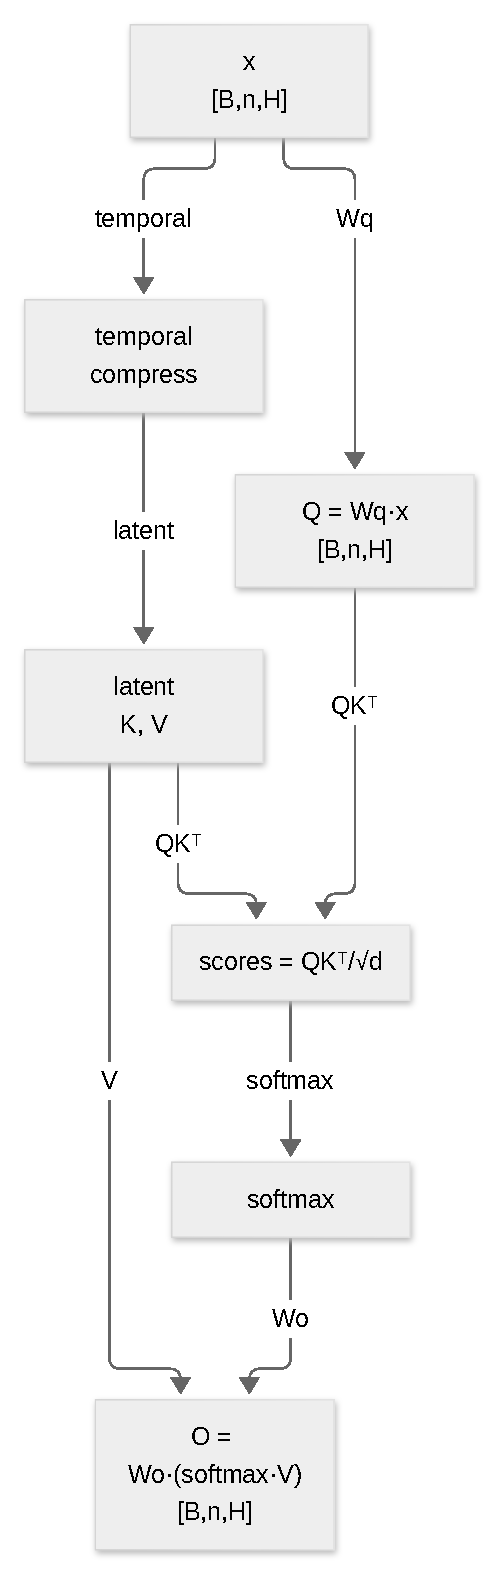
\includegraphics{../paper/figures/mixers/mtla.pdf}}
\caption{Flujo de datos de la atención latente temporal multi-cabeza: una etapa de compresión temporal produce el estado latente de clave/valor que atiende la consulta.}
\label{fig:mixer-mtla}
\end{figure}
La Atención Latente Temporal Multi-Cabeza (MTLA, por sus siglas en inglés) \citep{deng_mtla_2025} extiende MLA a lo largo del eje temporal: una hyper-red fusiona dinámicamente $m$ vectores temporalmente adyacentes del caché KV en un único slot, reduciendo la longitud temporal por un factor de $m$. Una máscara causal consciente del stride mantiene el entrenamiento paralelo consistente con la inferencia autorregresiva, produciendo una aceleración de decodificación de 5.3$\times$ y una reducción de memoria GPU de 8.3$\times$ frente a MHA en traducción de voz En--De.

\subsubsection{Formulación Matemática}
\[
c_{KV}^{(t)} = W_{DKV}\, x^{(t)} \in \mathbb{R}^{r_{kv}} \text{ (latente por token)}.
\]
\[
\bar c_{KV}^{(j)} = \sum_{i=0}^{m-1} \alpha_i\, c_{KV}^{(s j + i)}, \qquad \alpha_i = \texttt{sigmoid}(\text{HyperNet}(c_{KV}^{(s j + i)})),
\]
donde $s$ es el stride y $m$ la ventana de fusión. Las consultas atienden sobre slots fusionados $\bar c_{KV}$ con una máscara causal consciente del stride $M_{\text{stride}}$:
\[
\text{atencion} = \texttt{softmax}\!\left(\frac{q\, \bar k^\top}{\sqrt{d_h}} + M_{\text{stride}}\right) \bar v, \quad \bar k = W_{UK}\, \bar c_{KV},\ \bar v = W_{UV}\, \bar c_{KV}.
\]

\subsubsection{Pseudocódigo Algorítmico}
\begin{algorithmic}[1]
\State \textbf{Entrada:} latentes por token $c_{KV}^{(t)}$, ventana de fusión $m$, stride $s$
\State \textbf{Fase de fusión (hyper-red):}
\For{cada slot fusionado $j = 0, 1, \ldots$}
    \State $\alpha_i \gets \texttt{sigmoid}(\text{HyperNet}(c_{KV}^{(s j + i)}))$ para $i = 0, \ldots, m-1$
    \State $\bar c_{KV}^{(j)} \gets \sum_{i=0}^{m-1} \alpha_i\, c_{KV}^{(s j + i)}$ \Comment{promedio con compuerta sobre la ventana}
\EndFor
\State $\bar k \gets W_{UK}\, \bar c_{KV}$, \quad $\bar v \gets W_{UV}\, \bar c_{KV}$
\State $\text{pesos} \gets \texttt{softmax}(q\, \bar k^\top / \sqrt{d_h} + M_{\text{stride}})$ \Comment{máscara causal consciente del stride}
\State \textbf{Salida:} $\mathbf{Y} = \text{pesos} \cdot \bar v$
\end{algorithmic}

\subsubsection{Características Clave}
\begin{itemize}[leftmargin=*]
    \item \textbf{Complejidad de entrenamiento}: $\mathcal{O}(n^2 \cdot d / m)$ sobre la secuencia fusionada (longitud $\lceil n/m \rceil$) más costo de la hyper-red.
    \item \textbf{Complejidad de inferencia}: $\mathcal{O}(n/m)$ por token sobre slots fusionados; estado $\mathcal{O}(r_{kv} \cdot n / m)$.
    \item \textbf{Entrenable}: la hyper-red y la ventana de fusión $m$ se aprenden/eliges; la máscara consciente del stride garantiza consistencia.
    \item \textbf{Fortalezas}: aceleración de decodificación de 5.3$\times$, reducción de memoria GPU de 8.3$\times$ frente a MHA; compresión temporal ortogonal a la compresión de rango.
    \item \textbf{Limitaciones}: la ventana de fusión puede difuminar detalle temporal fino; la hyper-red añade cómputo; el diseño de la máscara no es trivial.
\end{itemize}

\subsection{Comparación y Síntesis Arquitectónica}

\subsection{Atención Convolucional Comprimida (CCA)}

\begin{figure}[H]
\centering
\fitfigure{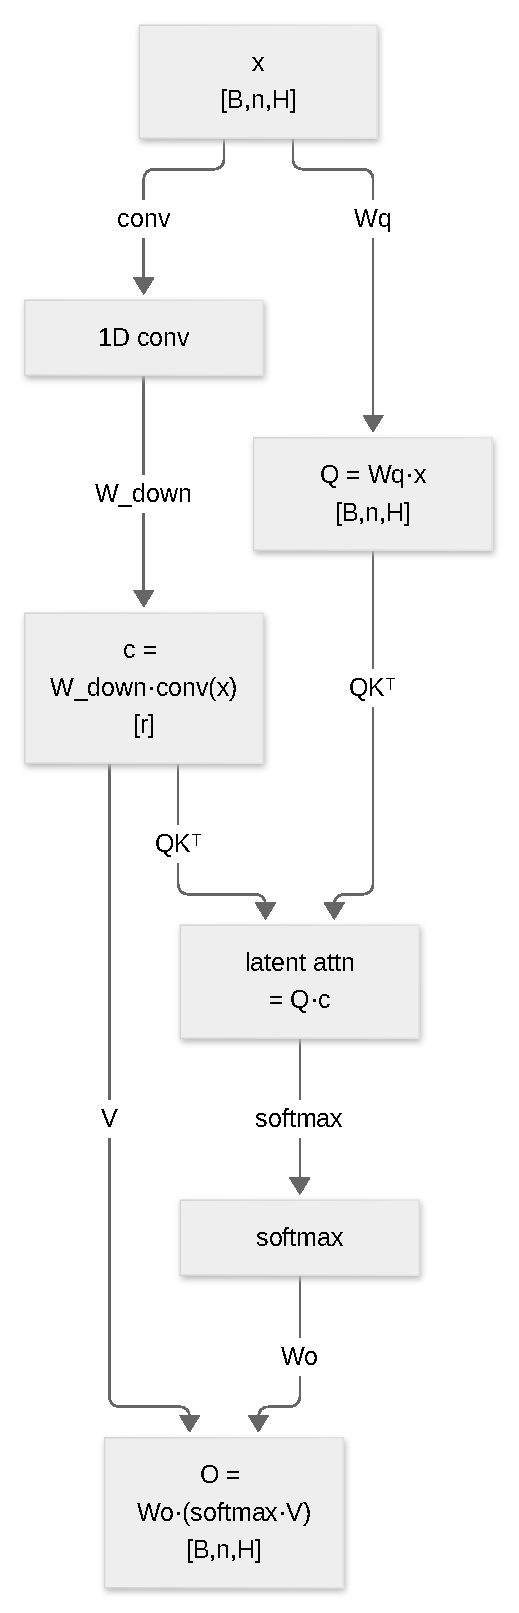
\includegraphics{../paper/figures/mixers/cca.pdf}}
\caption{Flujo de datos de la atención convolucional comprimida: una convolución 1D alimenta una compresión latente $c$ que la consulta atiende directamente.}
\label{fig:mixer-cca}
\end{figure}
La Atención Convolucional Comprimida (CCA, por sus siglas en inglés) \citep{figliola_cca_2025} adopta un enfoque fundamentalmente diferente para la atención latente: en lugar de comprimir el caché KV y luego up-proyectar al ancho completo antes de atender (como MLA/GQLA/MLRA), CCA proyecta consultas, claves y valores a un latente compartido y realiza la operación de atención \emph{completa} dentro de él. No hay matrices de up-proyección para Q/K/V --- sólo una única up-proyección de salida $\tilde{W}_O$ mapea la salida latente de vuelta al flujo residual. Esto reduce simultáneamente parámetros, caché KV, \textbf{y} FLOPs de atención por el factor de compresión $C = E/\tilde{e}$, mientras que MLA sólo reduce el caché.

Para hacer viable la atención en el latente comprimido, CCA introduce tres innovaciones: (1) dos convoluciones causales sobre el tensor empaquetado q/k (una convolución de secuencia depth-wise y una convolución agrupada de canales por cabeza), (2) q-k-mean (añade la media pre-convolución de q y k a los valores post-convolución), y (3) value-shift (cada cabeza recibe la mitad de sus valores del token actual y la mitad del token anterior mediante dos proyecciones independientes). Tras estos pasos, se aplica normalización L2 de QK y una temperatura de clave aprendible $\beta$, RoPE se aplica \emph{directamente en el latente} (sin cabeza RoPE separada), y se computa la atención softmax estándar.

\subsubsection{Formulación Matemática}
\[
\tilde{q}_{\text{pre}} = \tilde{W}_Q\, x, \qquad \tilde{k}_{\text{pre}} = \tilde{W}_K\, x, \qquad \tilde{e} = E / C.
\]
\[
\tilde{q} = \text{Conv}(\tilde{q}_{\text{pre}}) + \tfrac{1}{2}(\tilde{q}_{\text{pre}} + \tilde{k}_{\text{pre}}), \qquad
\tilde{k} = \text{Conv}(\tilde{k}_{\text{pre}}) + \tfrac{1}{2}(\tilde{q}_{\text{pre}} + \tilde{k}_{\text{pre}}).
\]
\[
\tilde{v} = [\tilde{W}_{V_1}\, x_t \;\|\; \tilde{W}_{V_2}\, x_{t-1}], \qquad
\hat{q} = \frac{\tilde{q} \sqrt{d_h}}{\|\tilde{q}\|}, \quad \hat{k} = \frac{\tilde{k} \sqrt{d_h}}{\|\tilde{k}\|} e^{\beta}.
\]
\[
\text{atencion} = \texttt{softmax}\!\left(\frac{\text{RoPE}(\hat{q})\, \text{RoPE}(\hat{k})^\top}{\sqrt{d_h}}\right) \tilde{v}, \qquad
\mathbf{Y} = \tilde{W}_O\, \text{atencion}.
\]

\subsubsection{Características Clave}
\begin{itemize}[leftmargin=*]
    \item \textbf{Complejidad de entrenamiento}: $\mathcal{O}(n^2 \cdot d / C)$ (atención en latente comprimido, $C{\times}$ menos FLOPs que MHA).
    \item \textbf{Complejidad de inferencia}: $\mathcal{O}(n)$ por token, espacio de caché KV $\mathcal{O}(\tilde{e} \cdot n)$.
    \item \textbf{Entrenable}: $C$, tamaños de kernel de conv, y los tres trucos (convs, qk-mean, value-shift) son configurables.
    \item \textbf{Fortalezas}: Reduce params, caché Y FLOPs simultáneamente; RoPE se integra nativamente; $>$2$\times$ menos params que MLA a igual compresión.
    \item \textbf{Limitaciones}: No elimina la cuadrática $S^2$ (sólo la divide por $C$); conv/qk-mean/v-shift añaden sesgo inductivo; se necesita kernel fusionado para la aceleración teórica.
\end{itemize}

\subsection{Atención Convolucional Comprimida por Consultas Agrupadas (CCGQA)}

\begin{figure}[H]
\centering
\fitfigure{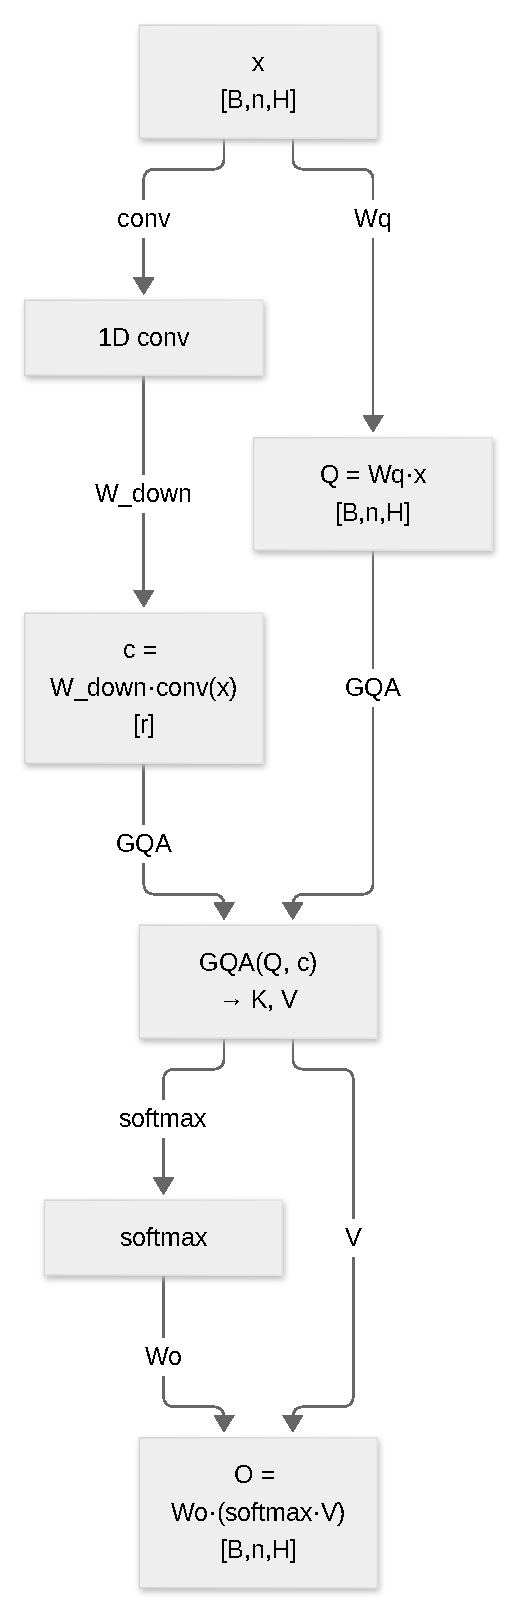
\includegraphics{../paper/figures/mixers/ccgqa.pdf}}
\caption{Flujo de datos de la atención convolucional comprimida con consultas agrupadas: el latente de la convolución alimenta una expansión de clave/valor con consultas agrupadas.}
\label{fig:mixer-ccgqa}
\end{figure}
La Atención Convolucional Comprimida por Consultas Agrupadas (CCGQA, por sus siglas en inglés) \citep{figliola_cca_2025} extiende CCA con compartición de cabezas clave/valor estilo GQA aplicada \emph{dentro} del latente comprimido, y \textbf{desacopla} las tasas de compresión de query y KV: las consultas se comprimen por $C_1$ y las claves/valores por $C_2 \geq C_1$. La dimensión latente por cabeza $d_h$ debe coincidir entre cabezas de query y clave, imponiendo la restricción $C_2 / C_1 = n_h / n_{kv}$. Las cabezas KV se comparten por grupo (replicadas para coincidir con las cabezas de query), y el sesgo qk-mean usa operadores de broadcast/reducción $B_{\text{group}}$ (replicar cabezas KV a cabezas query) y $E_{\text{group}}$ (promediar cabezas query dentro de cada grupo). CCGQA logra la mejor pérdida reportada a 8$\times$ reducción de caché KV sin pérdida de calidad frente a MHA.

\subsubsection{Características Clave}
\begin{itemize}[leftmargin=*]
    \item \textbf{Complejidad de entrenamiento}: $\mathcal{O}(n^2 \cdot d / C_1)$ (el término $S^2$ escala por $1/C_1$; los términos de proyección por $1/C_1 + 1/C_2$).
    \item \textbf{Complejidad de inferencia}: $\mathcal{O}(n)$ por token, espacio de caché KV $\mathcal{O}(\tilde{e}_{kv} \cdot n)$ (comprimido por $C_2$, compartido por grupo).
    \item \textbf{Entrenable}: $C_1$, $C_2$, $n_{kv}$, y todos los trucos CCA son configurables. Restricción: $C_2/C_1 = n_h/n_{kv}$.
    \item \textbf{Fortalezas}: Compresión desacoplada permite frontera de Pareto suave; misma intensidad aritmética que GQA; mejor pérdida a 8$\times$ reducción de caché.
    \item \textbf{Limitaciones}: Misma cuadrática $S^2$ (sólo reducida por $C_1$); se necesita kernel fusionado; dos proyecciones de valor añaden complejidad.
\end{itemize}

La familia latente muestra una progresión clara a lo largo de dos ejes: (i) \textbf{compresión de rango}, pasando de cabezas completas (MHA) a un latente compartido (MLA) a sub-cabezas latentes particionadas (MLRA), y (ii) \textbf{adaptividad de despliegue}, pasando de una sola ruta de decodificación a despacho adaptativo al hardware (GQLA) y fusión temporal de caché (MTLA). La Atención Tucker proporciona el marco algebraico unificador: MHA, GQA y MLA son todos casos especiales de una factorización Tucker con elecciones de rango apropiadas. CCA y CCGQA toman un enfoque fundamentalmente diferente: en lugar de comprimir el caché KV y luego up-proyectar para atención a ancho completo (MLA/GQLA/MLRA), realizan atención \emph{completamente dentro} del espacio latente comprimido, reduciendo no sólo el caché sino también los FLOPs de atención por el factor de compresión. CCGQA además desacopla las tasas de compresión de query y KV, logrando la mejor pérdida reportada a 8$\times$ reducción de caché KV. La Atención de Mezcla Gaussiana (GMA) cambia la filosofía de enrutamiento por completo: en lugar de un cuello de botella lineal de rango bajo, enruta a través de $K$ componentes Gaussianos probabilísticos aprendidos, logrando mezcla de secuencias en tiempo lineal $\mathcal{O}(NK)$ para $K$ fijo manteniendo una interpretación de atención normalizada.

\subsection{Atención de Mezcla Gaussiana (GMA)}

\begin{figure}[H]
\centering
\fitfigure{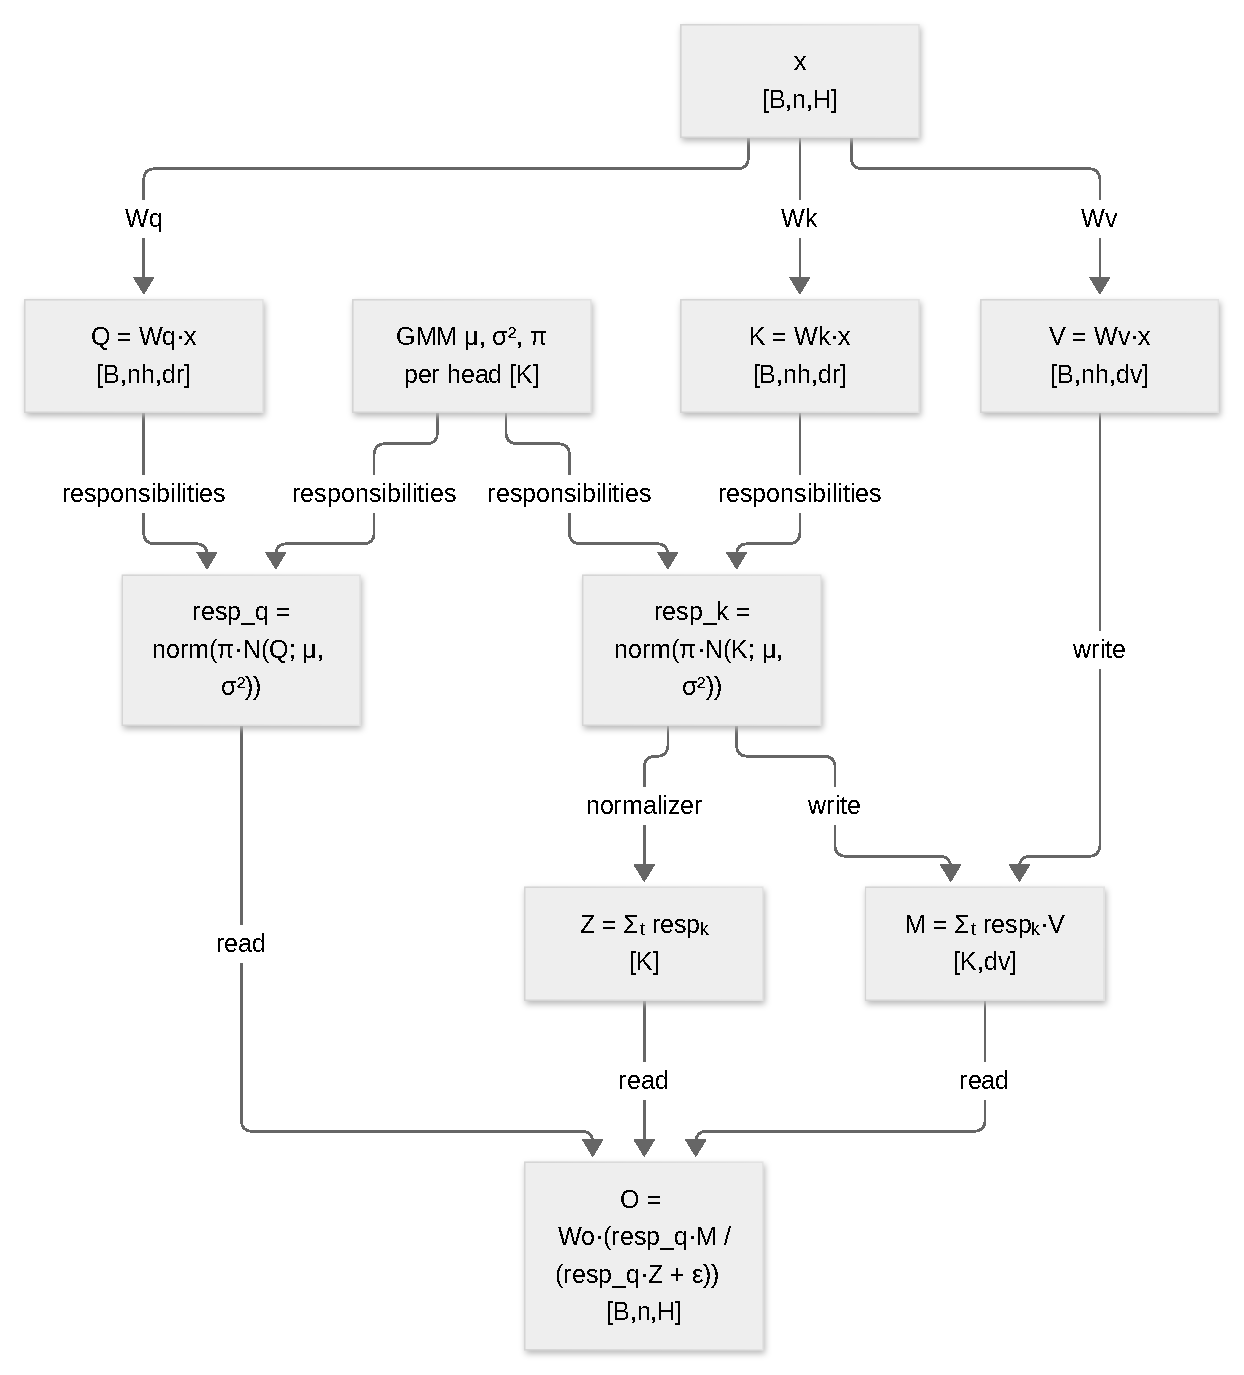
\includegraphics{../paper/figures/mixers/gma.pdf}}
\caption{Flujo de datos de la atención de mezcla gaussiana: las responsabilidades gaussianas por cabeza enrutan claves y valores hacia una memoria de $K$ ranuras que la consulta lee de vuelta, normalizada por $Z$.}
\label{fig:mixer-gma}
\end{figure}
La Atención de Mezcla Gaussiana (GMA, por sus siglas en inglés) \citep{huang_gma_2026} reemplaza la interacción pareada explícita $QK^\top$ de la atención de producto punto estándar con enrutamiento probabilístico a través de $K$ componentes de mezcla Gaussiana aprendidos por cabeza. Las consultas y claves se mapean a vectores de \emph{responsabilidad} posteriores sobre un espacio de enrutamiento latente compartido; su solapamiento define una afinidad implícita en el espacio de responsabilidades, mientras que los valores se escriben y leen de una memoria latente de $K$ slots. Al explotar la asociatividad de la multiplicación matricial, GMA evita materializar la matriz de afinidad $N \times N$ inducida y en su lugar usa dos matrices de responsabilidad $N \times K$ cuyo almacenamiento de activaciones dominante escala como $\mathcal{O}(NK)$ en lugar de $\mathcal{O}(N^2)$ para $K$ fijo. Los parámetros de la mezcla Gaussiana---medias de componentes $\mu$, covarianzas diagonales (reparametrizadas vía $\sigma^2 = \text{softplus}(\omega) + \epsilon_\sigma$) y logits de prior de mezcla $\alpha$ (con $\pi = \text{softmax}(\alpha)$)---son parámetros aprendibles totalmente diferenciables optimizados por retropropagación estándar, sin bucle EM ni pérdida auxiliar de clustering.

\subsubsection{Formulación Matemática}
Por cabeza, con dimensión de enrutamiento $d_r$ y dimensión de valor $d_v$:
\[
Q_X = X W_Q \in \mathbb{R}^{N \times d_r}, \quad
K_X = X W_K \in \mathbb{R}^{N \times d_r}, \quad
V_X = X W_V \in \mathbb{R}^{N \times d_v}.
\]
La responsabilidad posterior del componente $k$ para un vector de enrutamiento $x_i$ es
\[
\gamma_{i,k} = p(z{=}k \mid x_i) = \frac{\pi_k\, \mathcal{N}(x_i \mid \mu_k, \Sigma_k)}{\sum_{\ell=1}^{K} \pi_\ell\, \mathcal{N}(x_i \mid \mu_\ell, \Sigma_\ell)},
\qquad \Sigma_k = \mathrm{diag}(\sigma_{k,1}^2, \dots, \sigma_{k,d_r}^2),
\]
produciendo las matrices de responsabilidad $\Gamma^Q, \Gamma^K \in \mathbb{R}^{N \times K}$. La salida bidireccional se calcula mediante el par asociativo de escritura--lectura
\[
\tilde V = (\Gamma^K)^\top V_X \in \mathbb{R}^{K \times d_v}, \qquad
Z = (\Gamma^K)^\top \mathbf{1}_N \in \mathbb{R}^{K}, \qquad
O = \frac{\Gamma^Q \tilde V}{\Gamma^Q Z + \epsilon},
\]
que nunca materializa la afinidad normalizada implícita $A^{\text{GMA}}_{ij} = \frac{\sum_k \gamma^Q_{i,k} \gamma^K_{j,k}}{\sum_\ell \sum_k \gamma^Q_{i,k} \gamma^K_{\ell,k} + \epsilon}$. Para modelado autorregresivo, las estadísticas de escritura globales se reemplazan por sumas acumuladas restringidas al prefijo $\tilde V^{(i)}_k = \sum_{j \le i} \gamma^K_{j,k} V_{X,j}$ y $Z^{(i)}_k = \sum_{j \le i} \gamma^K_{j,k}$, imponiendo causalidad preservando el escalado lineal de $K$ fijo.

\subsubsection{Pseudocódigo Algorítmico}
\begin{algorithmic}[1]
\State \textbf{Entrada:} estado oculto $X \in \mathbb{R}^{N \times d}$, $K$ componentes, dim. de enrutamiento $d_r$, dim. de valor $d_v$, params $\{\mu_k, \omega_k, \alpha_k\}_{k=1}^{K}$
\State $Q_X \gets X W_Q$, \quad $K_X \gets X W_K$, \quad $V_X \gets X W_V$ \Comment{proyecciones por cabeza}
\State $\sigma^2_k \gets \text{softplus}(\omega_k) + \epsilon_\sigma$, \quad $\pi_k \gets \text{softmax}(\alpha)_k$ \Comment{reparametrizar}
\State $\Gamma^Q \gets \texttt{softmax}_k\!\left(\log \pi_k - \tfrac{d_r}{2}\log 2\pi - \tfrac{1}{2}\sum_m \log \sigma^2_{k,m} - \tfrac{1}{2}\sum_m \frac{(q_{i,m}-\mu_{k,m})^2}{\sigma^2_{k,m}}\right)$
\State $\Gamma^K \gets$ igual que $\Gamma^Q$ aplicado a $K_X$
\If{causal}
    \State $\tilde V \gets \texttt{cumsum}_n(\Gamma^K \otimes V_X)$, \quad $Z \gets \texttt{cumsum}_n(\Gamma^K)$ \Comment{restringido al prefijo}
\Else
    \State $\tilde V \gets (\Gamma^K)^\top V_X$, \quad $Z \gets (\Gamma^K)^\top \mathbf{1}_N$ \Comment{escritura global}
\EndIf
\State $O \gets \Gamma^Q \tilde V \,/\, (\Gamma^Q Z + \epsilon)$ \Comment{lectura normalizada}
\State \textbf{Salida:} $\mathbf{Y} = O W_O$
\end{algorithmic}

\subsubsection{Características Clave}
\begin{itemize}[leftmargin=*]
    \item \textbf{Complejidad de entrenamiento}: $\mathcal{O}(N K d_r + N K d_v)$ para $K$ fijo, lineal en la longitud de secuencia $N$.
    \item \textbf{Complejidad de inferencia}: $\mathcal{O}(K)$ por token (responsabilidades + lectura latente), almacenamiento de activaciones $\mathcal{O}(NK)$.
    \item \textbf{Entrenable}: parámetros GMM totalmente diferenciables $\{\mu, \omega, \alpha\}$ por cabeza, optimizados end-to-end sin EM.
    \item \textbf{Fortalezas}: Mezcla de secuencias en tiempo lineal con $K$ fijo; enrutamiento probabilístico interpretable; variantes bidireccional y causal; interpretación de afinidad de rango bajo no negativa $A^{\text{GMA}} = \mathrm{diag}(d)^{-1} \Gamma^Q (\Gamma^K)^\top$.
    \item \textbf{Limitaciones}: La calidad depende de $K$ y la dimensión de enrutamiento $d_r$; la GMA causal queda por debajo de SDPA optimizada y modelos de espacio de estados en WikiText-103 en la implementación actual del paper; no es un reemplazo universal para la atención softmax.
\end{itemize}
\section{Mecanismos de Atención Dispersa Exhaustivos}
\label{sec:annex-sparse}

\subsection{Resumen Ejecutivo}

Los mecanismos de atención dispersa abordan la prohibitiva complejidad computacional y de memoria $\mathcal{O}(n^2)$ de la atención de producto punto escalado estándar al restringir el conjunto de pares clave-valor atendidos. La atención dispersa moderna abarca un rico espacio de diseño distinguido por cuatro dimensiones ortogonales: (i) \textbf{patrón de dispersidad} (geométrico fijo, dependiente de datos o basado en frecuencia), (ii) \textbf{capacidad de entrenamiento} (entrenado de extremo a extremo o solo inferencia), (iii) \textbf{unidad de dispersidad} (tokens individuales, ventanas locales o bloques), y (iv) \textbf{mecanismo} (enmascaramiento, selección, filtrado o compresión). Este anexo sintetiza diez familias principales de atención dispersa---Sparse Transformer, Longformer, SWA con sumideros de atención, BigBird, SparseK, NSA, FASA, SpargeAttn, MSA y SparDA---proporcionando formulaciones matemáticas, pseudocódigo algorítmico y comparaciones arquitectónicas exhaustivas.

\subsection{Sparse Transformer: Patrones Estrideados y Fijos Factorizados}

\begin{figure}[H]
\centering
\fitfigure{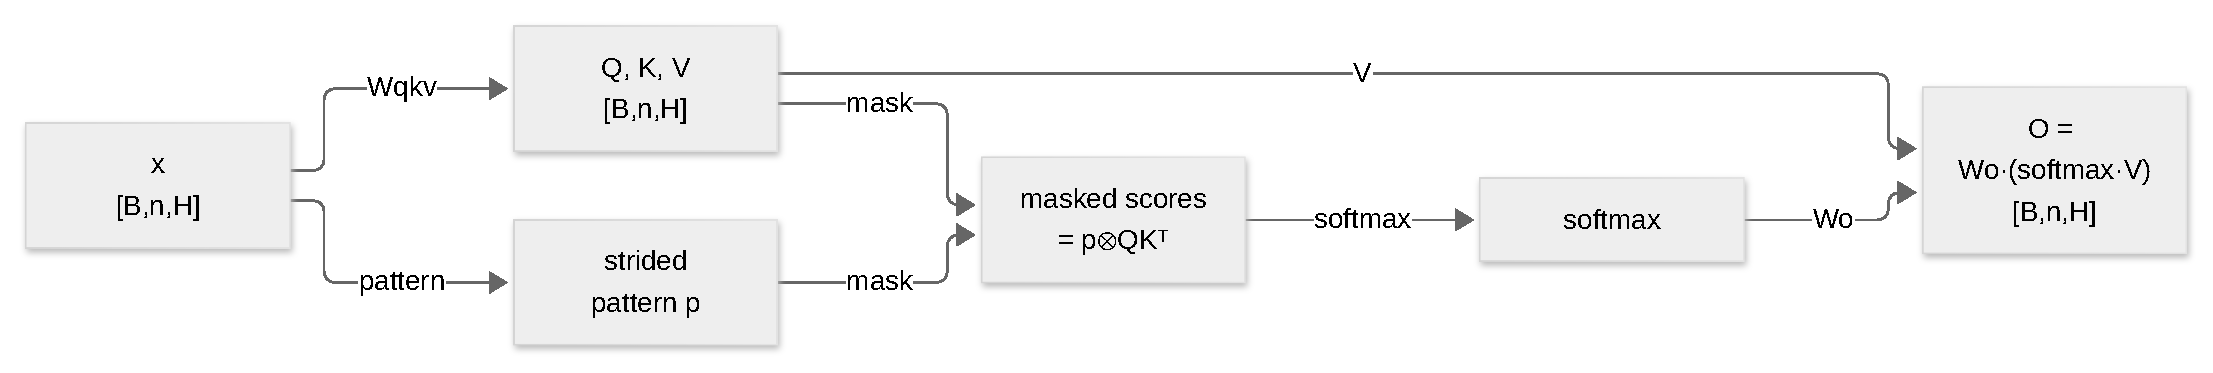
\includegraphics{../paper/figures/mixers/sparse-transformer.pdf}}
\caption{Flujo de datos del Sparse Transformer: un patrón factorial con zancada enmascara la matriz de puntuaciones antes del softmax.}
\label{fig:mixer-sparse-transformer}
\end{figure}

\subsubsection{Formulación Matemática}

Sparse Transformer \citep{child_sparse_transformer_2019} reduce la complejidad cuadrática a $\mathcal{O}(n\sqrt{n})$ factorizando la atención dispersa en dos cabezas dispersas complementarias. Sea $n$ la longitud de la secuencia y $l = \lfloor\sqrt{n}\rfloor$ el stride.

\paragraph{Cabeza de atención estrideada}: Cada posición $i$ atiende a cada $l$-ésima posición anterior:
\[
\mathcal{A}_i^{(\text{estrideada})} = \{j : j \leq i,\; (i - j) \bmod l = 0\}
\]

\paragraph{Cabeza de atención fija}: Cada posición $i$ atiende a posiciones dentro de su bloque local más columnas de resumen fijas:
\[
\mathcal{A}_i^{(\text{fija})} = \{j : \lfloor j/l \rfloor = \lfloor i/l \rfloor\} \cup \{j : j \bmod l \in \{l-c, \ldots, l-1\}\}
\]
donde $c$ es un hiperparámetro que controla el número de columnas de resumen (típicamente $c=1$ o $c=2$).

El cálculo de atención para cada cabeza $h$ sigue las reglas estándar de producto punto escalado restringido al conjunto disperso:
\[
\text{Attn}_h(Q, K, V)_i = \text{softmax}\left(\frac{q_i^h K_{\mathcal{A}_i}^h\top}{\sqrt{d_k}}\right) V_{\mathcal{A}_i}^h
\]

La idea clave es que con las dos cabezas factorizadas operando en paralelo a través de una profundidad de $L$ capas transformer, cada posición puede alcanzar cualquier otra posición a través de un camino de longitud máxima $L + 1$, preservando la alcanzabilidad de largo alcance con una fracción del costo de la atención densa.

\subsubsection{Pseudocódigo Algorítmico}

\begin{algorithm}[H]
\caption{Atención Sparse Transformer: Cabezas Duales Estrideada + Fija}
\begin{algorithmic}[1]
\Require Consulta $\mathbf{Q} \in \mathbb{R}^{n \times d}$, Clave $\mathbf{K} \in \mathbb{R}^{n \times d}$, Valor $\mathbf{V} \in \mathbb{R}^{n \times d}$
\Require Stride $l = \lfloor\sqrt{n}\rfloor$, columnas de resumen $c \in \{1, 2\}$
\Ensure Salida $\mathbf{Y} \in \mathbb{R}^{n \times d}$
\State \textbf{Cabeza 1: Atención Estrideada}
\For{$i = 1, \ldots, n$}
    \State $\mathcal{A}_i \gets \{j : j \leq i \text{ y } (i-j) \bmod l = 0\}$ \Comment{Cada $l$-ésima posición}
    \State $\text{puntajes}_{i} \gets \mathbf{q}_i \mathbf{K}_{\mathcal{A}_i}^\top / \sqrt{d_k}$
    \State $\text{attn}_{i} \gets \text{softmax}(\text{puntajes}_{i})$
    \State $\mathbf{y}_i^{(1)} \gets \text{attn}_{i} \mathbf{V}_{\mathcal{A}_i}$
\EndFor
\State \textbf{Cabeza 2: Atención de Bloque Fijo + Resumen}
\For{$i = 1, \ldots, n$}
    \State $\text{inicio\_bloque} \gets \lfloor i/l \rfloor \cdot l$, $\text{fin\_bloque} \gets \min(i+1, \text{inicio\_bloque}+l)$
    \State $\mathcal{A}_i \gets [\text{inicio\_bloque}, \text{fin\_bloque}) \cup \{\text{columnas de las últimas } c \text{ columnas}\}$
    \State $\text{puntajes}_{i} \gets \mathbf{q}_i \mathbf{K}_{\mathcal{A}_i}^\top / \sqrt{d_k}$
    \State $\text{attn}_{i} \gets \text{softmax}(\text{puntajes}_{i})$
    \State $\mathbf{y}_i^{(2)} \gets \text{attn}_{i} \mathbf{V}_{\mathcal{A}_i}$
\EndFor
\State Concatenar: $\mathbf{Y} = [\mathbf{y}^{(1)} \| \mathbf{y}^{(2)}]$ y proyectar mediante capa lineal de salida
\Return $\mathbf{Y}$
\end{algorithmic}
\end{algorithm}

\subsubsection{Características Clave}

\begin{itemize}[leftmargin=*]
    \item \textbf{Complejidad}: $\mathcal{O}(n\sqrt{n} \cdot d)$ durante el entrenamiento; $\mathcal{O}(n)$ por token durante la generación.
    \item \textbf{Entrenable}: Sí; retropropagación completa a través de las posiciones seleccionadas.
    \item \textbf{Patrón de dispersidad}: Fijo e independiente de los datos; los patrones no se adaptan al contenido.
    \item \textbf{Fortaleza}: Alcanzabilidad estructurada que garantiza dependencias de largo alcance; demostrado efectivo en secuencias largas (Enwik8, imágenes de texto).
    \item \textbf{Limitación}: Los patrones fijos pueden pasar por alto relaciones importantes pero no contiguas; requiere kernels CUDA personalizados para eficiencia práctica.
\end{itemize}

\subsection{Longformer: Ventana Deslizante, Dilatación y Tokens Globales}

\begin{figure}[H]
\centering
\fitfigure{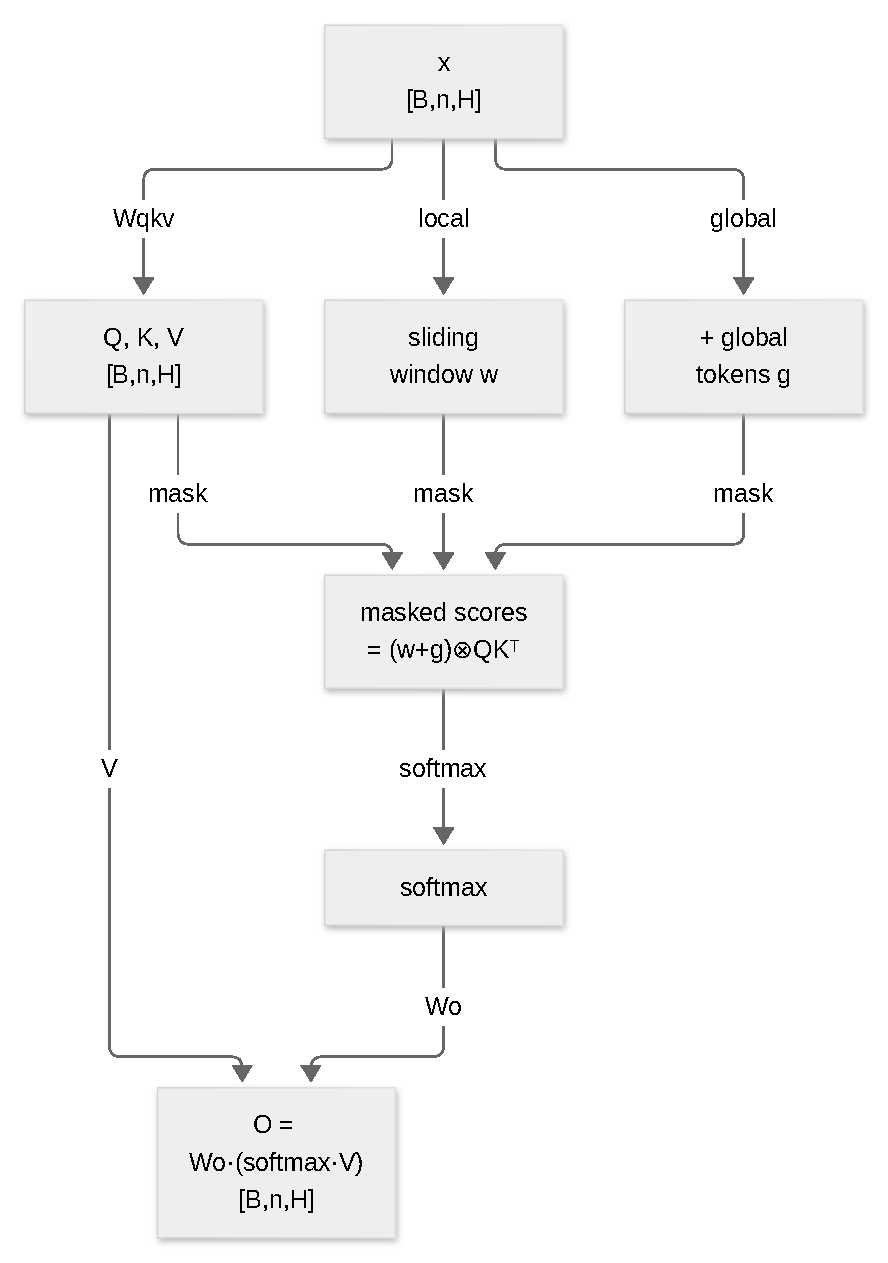
\includegraphics{../paper/figures/mixers/longformer.pdf}}
\caption{Flujo de datos de Longformer: las máscaras de ventana deslizante y de tokens globales se aplican a la matriz de puntuaciones antes del softmax.}
\label{fig:mixer-longformer}
\end{figure}

\subsubsection{Formulación Matemática}

Longformer \citep{beltagy_longformer_2020} logra una complejidad lineal $\mathcal{O}(n \cdot w)$ combinando tres patrones de atención complementarios.

\paragraph{Atención de ventana deslizante}: Vecindario local de tamaño $w$:
\[
\mathcal{A}_i^{(\text{ventana})} = \{j : |i - j| \leq w/2\}
\]

\paragraph{Ventana deslizante dilatada}: Atención con ventana y dilatación $d$, saltando stride $d+1$:
\[
\mathcal{A}_i^{(\text{dilatada})} = \{j : |i - j| \leq (w/2)(d+1) \text{ y } (i-j) \bmod (d+1) = 0\}
\]

\paragraph{Atención global}: Tokens globales designados (ej., $[\text{CLS}]$) atienden a todas las posiciones y todos atienden a ellos:
\[
\mathcal{A}_i^{(\text{global})} = \begin{cases}
\{1, \ldots, n\} & \text{si } i \in \mathcal{G} \\
\mathcal{A}_i^{(\text{ventana})} \cup \mathcal{G} & \text{en otro caso}
\end{cases}
\]

Los tres patrones se aplican mediante proyecciones separadas. La atención local y global pueden usar las mismas proyecciones o unas separadas específicas para cada tarea.

\subsubsection{Pseudocódigo Algorítmico}

\begin{algorithm}[H]
\caption{Longformer: Ventana Deslizante + Dilatada + Global}
\begin{algorithmic}[1]
\Require Consulta $\mathbf{Q} \in \mathbb{R}^{n \times d}$, Clave $\mathbf{K}$, Valor $\mathbf{V}$, tamaño de ventana $w$, dilatación $d$, índices de tokens globales $\mathcal{G}$
\Ensure Salida $\mathbf{Y}$
\For{$i = 1, \ldots, n$}
    \If{$i \in \mathcal{G}$}
        \State $\mathcal{A}_i \gets \{1, \ldots, n\}$ \Comment{Token global atiende a todos}
    \Else
        \State Ventana local: $\mathcal{A}^{(\text{local})} \gets [i - w/2, i + w/2] \cap [1, n]$
        \State Desplazamientos dilatados: $\mathcal{A}^{(\text{dilatada})} \gets \{j : (i-j) \bmod (d+1) = 0\} \cap \mathcal{A}^{(\text{rango dilatado})}$
        \State Combinar: $\mathcal{A}_i \gets \mathcal{A}^{(\text{local})} \cup \mathcal{A}^{(\text{dilatada})} \cup \mathcal{G}$
    \EndIf
    \State $\text{puntajes}_i \gets \mathbf{q}_i \mathbf{K}_{\mathcal{A}_i}^\top / \sqrt{d_k}$
    \State $\text{attn}_i \gets \text{softmax}(\text{puntajes}_i)$
    \State $\mathbf{y}_i \gets \text{attn}_i \mathbf{V}_{\mathcal{A}_i}$
\EndFor
\Return $\mathbf{Y}$
\end{algorithmic}
\end{algorithm}

\subsubsection{Características Clave}

\begin{itemize}[leftmargin=*]
    \item \textbf{Complejidad}: $\mathcal{O}(n \cdot w)$ donde $w$ es el tamaño de ventana (lineal cuando $w \ll n$).
    \item \textbf{Entrenable}: Sí; reemplazo directo para la atención estándar.
    \item \textbf{Cobertura}: Con $L$ capas y tamaño de ventana $w$, el campo receptivo crece a $L \times w$, cubriendo toda la secuencia con redes poco profundas.
    \item \textbf{Fortaleza}: Práctico para tareas a nivel de documentos; la dilatación expande los campos receptivos locales con sobrecarga mínima; los tokens globales proporcionan correspondencia consulta-documento.
    \item \textbf{Limitación}: El tamaño de ventana sigue siendo un hiperparámetro de diseño; subóptimo para tareas que requieren patrones de atención densos.
\end{itemize}

\subsection{SWA con Sumideros de Atención: Ventana Deslizante Más un Prefijo Sumidero}

\begin{figure}[H]
\centering
\fitfigure{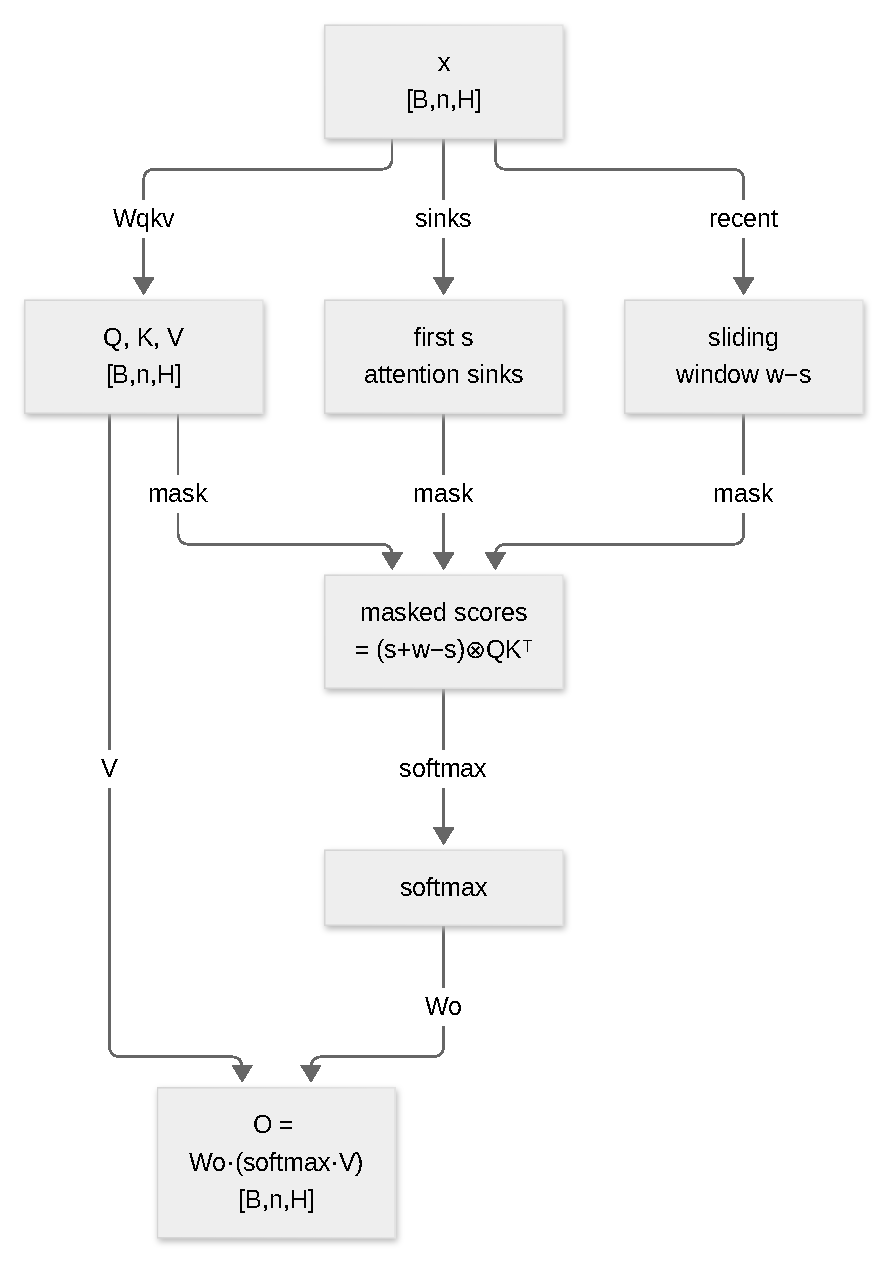
\includegraphics{../paper/figures/mixers/swa.pdf}}
\caption{Flujo de datos de SWA con sumideros de atención: los primeros $s$ tokens sumidero y una ventana deslizante causal de $w-s$ se unen en una máscara aplicada a la matriz de puntuaciones antes del softmax.}
\label{fig:mixer-swa}
\end{figure}

\subsubsection{Formulación Matemática}

SWA con sumideros de atención \citep{jolicoeur_sliding_window_2026} es la política de desalojo de caché KV más simple: en lugar de comprimir la caché o reemplazar la atención por un estado recurrente, restringe cada consulta a un conjunto pequeño y fijo de claves. Denotemos el tamaño de ventana $w$ y el número de sumideros $s$, es decir $\mathrm{SWA}(w,s)$. En modo decoder, la consulta $i$ atiende a
\[
\mathcal{A}_i = \underbrace{\{j : j < s,\; j \leq i\}}_{\text{sumideros de atención}} \;\cup\; \underbrace{\{j : i - (w-s) + 1 \leq j \leq i\}}_{\text{ventana deslizante de } w-s},
\]
de modo que cada consulta ve como máximo $w$ claves. El recorte causal $j \leq i$ sobre el término de sumideros es esencial: los tokens anteriores a la posición $s$ no deben ver sumideros futuros.

\paragraph{Por qué los sumideros son imprescindibles} Los transformers aprenden a asignar una masa de atención desproporcionadamente grande a los primeros tokens aunque no sean semánticamente relevantes. Estos \emph{sumideros de atención} \citep{xiao_streaming_sinks_2024} actúan como repositorios de la atención sobrante. Cuando el prefijo sale de una ventana deslizante sin sumideros, el modelo pierde su destino de descarga y la calidad colapsa catastróficamente; reincluir los primeros $s$ tokens recupera la mayor parte del rendimiento de la atención completa. El paper fija $s = 4$ y evalúa $w \in \{64, 128, 256, 512\}$.

\paragraph{Extensión a encoder} El paper define $\mathrm{SWA}(w,s)$ para modelos de lenguaje causales. Para encoders bidireccionales la ventana local se hace simétrica, $\{j : |i-j| \leq \lfloor (w-s)/2 \rfloor\}$, y se une con el prefijo sumidero---la misma convención que usa Longformer.

Como la intervención es un cambio puro de máscara de atención, no requiere parámetros adicionales ni matemática QKV nueva: se reutilizan las proyecciones estándar $W_q, W_k, W_v, W_o$. Puede aplicarse a un checkpoint preentrenado en inferencia con cero tokens de entrenamiento, o entrenarse desde cero como un mixer normal.

\subsubsection{Pseudocódigo Algorítmico}

\begin{algorithm}[H]
\caption{SWA con Sumideros de Atención: Construcción de Máscara y Atención}
\begin{algorithmic}[1]
\Require Consulta $\mathbf{Q} \in \mathbb{R}^{n \times d}$, Clave $\mathbf{K}$, Valor $\mathbf{V}$, ventana $w$, sumideros $s$
\Ensure Salida $\mathbf{Y} \in \mathbb{R}^{n \times d}$
\State Índices de fila $i$, índices de columna $j$
\State $\text{causal} \gets [j \leq i]$
\State $\text{sumideros} \gets [j < s] \wedge \text{causal}$ \Comment{Prefijo sumidero recortado causalmente}
\State $\text{ventana} \gets [i - (w-s) + 1 \leq j \leq i]$
\State $M \gets \text{sumideros} \lor \text{ventana}$
\State $S \gets \mathbf{Q}\mathbf{K}^{\top} / \sqrt{d_k}$
\State $S \gets \text{mask}(S, M)$ \Comment{$-\infty$ donde $M = 0$}
\State $\mathbf{Y} \gets \text{softmax}(S)\, \mathbf{V}$
\Return $\mathbf{Y}$
\end{algorithmic}
\end{algorithm}

\subsubsection{Características Clave}

\begin{itemize}[leftmargin=*]
    \item \textbf{Complejidad}: $\mathcal{O}(n \cdot w \cdot d)$ en tiempo y $\mathcal{O}(w)$ de almacenamiento KV por capa en inferencia (fijo una vez que la secuencia supera $w$).
    \item \textbf{Entrenable}: Ambos; sin entrenamiento en inferencia sobre checkpoints preentrenados, o entrenado desde cero.
    \item \textbf{Campo receptivo}: Tras $L$ capas, $L(w-s)$ posiciones más el prefijo sumidero siempre visible.
    \item \textbf{Fortaleza}: Recupera $\approx 99\%$ de la puntuación media de atención completa en modelos de 1.3B a 72B con cero tokens de entrenamiento, y supera a la atención lineal retrofiteada por 2--10$\times$ en razonamiento de contexto largo (S-NIAH, BABILong) decodificando más rápido y usando menos memoria.
    \item \textbf{Limitación}: El horizonte es fijo y depende de la tarea---$w=64$ basta para benchmarks de verosimilitud pero colapsa en matemáticas generativas, donde se necesita $w=512$; no hay selección adaptativa al contenido.
\end{itemize}

\subsection{BigBird: Grafo Disperso Aleatorio, Local y Global}

\begin{figure}[H]
\centering
\fitfigure{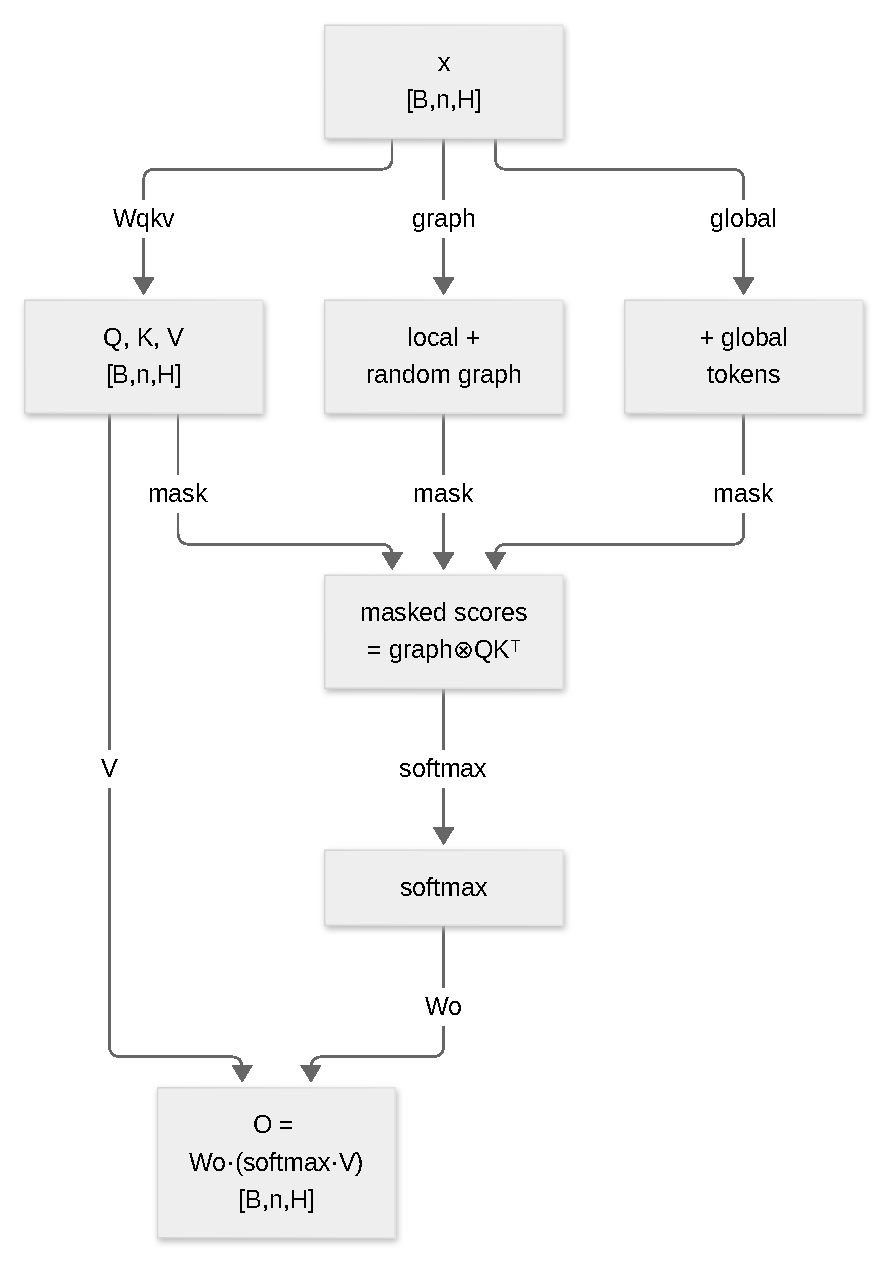
\includegraphics{../paper/figures/mixers/bigbird.pdf}}
\caption{Flujo de datos de BigBird: la adyacencia local, aleatoria y global enmascara la matriz de puntuaciones antes del softmax.}
\label{fig:mixer-bigbird}
\end{figure}

\subsubsection{Formulación Matemática}

BigBird \citep{zaheer_bigbird_2020} preserva la aproximación universal y la completitud de Turing utilizando una combinación fundamentada de tres patrones de dispersidad.

\paragraph{Conexiones aleatorias}: Cada posición se conecta a $r$ posiciones muestreadas aleatoriamente:
\[
\mathcal{A}_i^{(\text{aleatoria})} = \text{MuestraAleatoria}(\{1, \ldots, n\}, r)
\]

\paragraph{Ventana local}: Vecindario de ventana deslizante:
\[
\mathcal{A}_i^{(\text{local})} = \{j : |i-j| \leq w/2\}
\]

\paragraph{Tokens globales}: Anclas globales específicas de la tarea:
\[
\mathcal{A}_i^{(\text{global})} = \begin{cases}
\{1, \ldots, n\} & \text{si } i \in \mathcal{G} \\
\mathcal{A}_i^{(\text{aleatoria})} \cup \mathcal{A}_i^{(\text{local})} \cup \mathcal{G} & \text{en otro caso}
\end{cases}
\]

La máscara dispersa compuesta $M$ es:
\[
M_{ij} = \mathbf{1}[j \in \mathcal{A}_i^{(\text{aleatoria})} \cup \mathcal{A}_i^{(\text{local})} \cup \mathcal{A}_i^{(\text{global})}]
\]

En la práctica, BigBird agrupa tokens en bloques de tamaño $b$ y aplica la decisión de dispersidad a nivel de bloque, permitiendo implementaciones eficientes de bloques dispersos.

\subsubsection{Garantía Teórica}

Los autores demuestran que con $O(1)$ conexiones aleatorias y tokens globales, el grafo disperso mantiene las mismas propiedades de aproximación universal y completitud de Turing que la atención densa. Formalmente, cualquier función computable puede representarse y cualquier secuencia de operaciones puede simularse dentro del grafo de conectividad de BigBird.

\subsubsection{Pseudocódigo Algorítmico}

\begin{algorithm}[H]
\caption{BigBird: Atención Dispersa por Bloques Aleatoria + Local + Global}
\begin{algorithmic}[1]
\Require Consulta $\mathbf{Q}$, Clave $\mathbf{K}$, Valor $\mathbf{V}$, tamaño de bloque $b$, enlaces aleatorios por bloque $r$, índices globales $\mathcal{G}$
\Ensure Salida $\mathbf{Y}$
\State Reformar en bloques: $n_b = \lceil n / b \rceil$ bloques
\For{bloque $i = 0, \ldots, n_b-1$}
    \For{posición $j$ en bloque $i$}
        \State \textbf{Ventana local}: $\mathcal{A}_j^{(\text{local})} = \text{posiciones cercanas en el bloque} \cup \text{posiciones frontera}$
        \State \textbf{Muestreo aleatorio de bloques}: Muestrear $r$ bloques uniformemente al azar, agregar todas las posiciones de esos bloques
        \State \textbf{Global}: Agregar todas las posiciones de tokens globales
        \State $\mathcal{A}_j \gets \mathcal{A}_j^{(\text{local})} \cup \mathcal{A}_j^{(\text{aleatoria})} \cup \mathcal{G}$
    \EndFor
\EndFor
\For{$i = 1, \ldots, n$}
    \State $\text{puntajes}_i \gets \mathbf{q}_i \mathbf{K}_{\mathcal{A}_i}^\top / \sqrt{d_k}$
    \State $\text{attn}_i \gets \text{softmax}(\text{puntajes}_i)$
    \State $\mathbf{y}_i \gets \text{attn}_i \mathbf{V}_{\mathcal{A}_i}$
\EndFor
\Return $\mathbf{Y}$
\end{algorithmic}
\end{algorithm}

\subsubsection{Características Clave}

\begin{itemize}[leftmargin=*]
    \item \textbf{Complejidad}: $\mathcal{O}(n)$ o casi lineal en implementación óptima de bloques dispersos.
    \item \textbf{Entrenable}: Sí.
    \item \textbf{Base teórica}: Mantiene demostrablemente la aproximación universal y la completitud de Turing con conectividad dispersa.
    \item \textbf{Fortaleza}: Rendimiento sólido en documentos largos para preguntas-respuestas, resúmenes y tareas de genómica.
    \item \textbf{Limitación}: El muestreo aleatorio introduce varianza y no determinismo; el ajuste de los hiperparámetros $r, w, g$ sigue dependiendo de la tarea.
\end{itemize}

\subsection{Atención SparseK: Selección Diferencial \texorpdfstring{Top-$k$}{Top-k}}

\begin{figure}[H]
\centering
\fitfigure{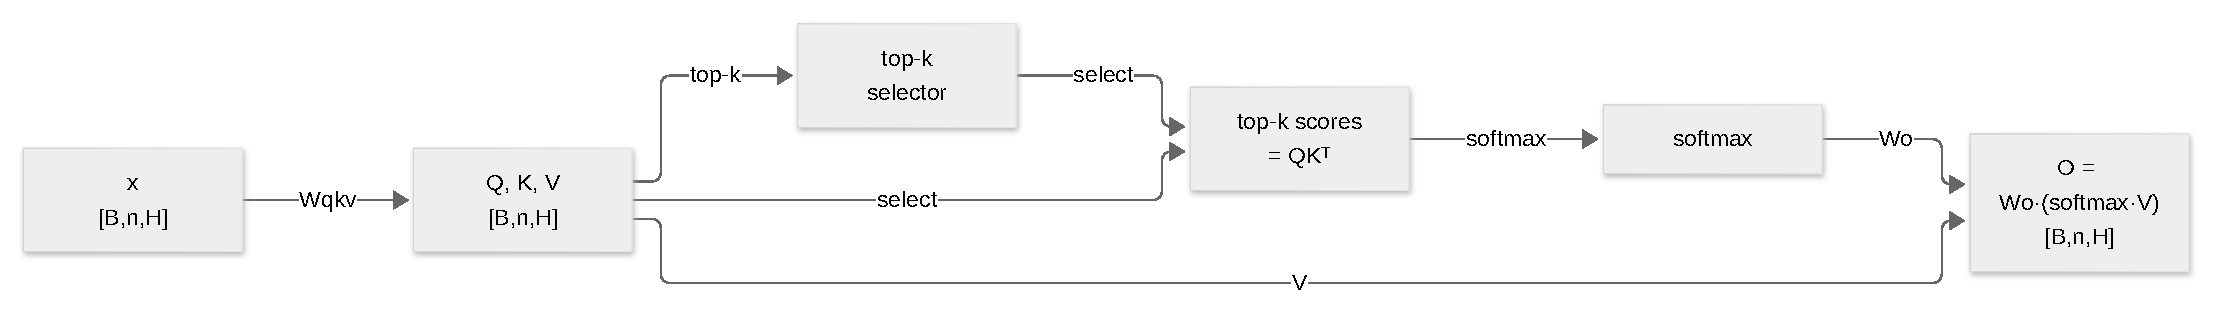
\includegraphics{../paper/figures/mixers/sparsek.pdf}}
\caption{Flujo de datos de SparseK: un selector top-$k$ diferenciable conserva solo las claves con mayor puntuación antes del softmax.}
\label{fig:mixer-sparsek}
\end{figure}

\subsubsection{Formulación Matemática}

SparseK \citep{lou_sparsek_2024} permite dispersidad aprendible mediante un \textbf{operador top-$k$ diferenciable}. Una red de puntuación $\phi_\theta$ evalúa la importancia de cada par clave-valor:

\[
u_j = \phi_\theta(\mathbf{k}_j, \mathbf{q}_i) \in \mathbb{R}
\]

El \textbf{operador SparseK} selecciona los puntajes top-$k$ manteniéndose diferenciable. Calcula un umbral $\tau(u)$ tal que la suma de los puntajes activos sea igual a $k$:

\[
\text{SparseK}(u, k)_j = \max(u_j - \tau(u), 0), \quad \text{donde} \quad \sum_j \max(u_j - \tau, 0) = k
\]

El umbral $\tau$ se encuentra mediante bisección. La atención se convierte en:

\[
m_j = \text{SparseK}(u, k)_j, \quad \text{Attn}_i = \text{softmax}\left(\frac{\mathbf{q}_i K_{\text{sel}}^\top}{\sqrt{d_k}}\right) V_{\text{sel}}
\]

donde $K_{\text{sel}}, V_{\text{sel}}$ contienen solo las entradas top-$k$ (aquellas con $m_j > 0$).

\subsubsection{Pseudocódigo Algorítmico}

\begin{algorithm}[H]
\caption{SparseK: Atención Top-$k$ Diferenciable}
\begin{algorithmic}[1]
\Require Consulta $\mathbf{q} \in \mathbb{R}^d$, Matriz de clave $\mathbf{K} \in \mathbb{R}^{n \times d}$, Matriz de valor $\mathbf{V} \in \mathbb{R}^{n \times d}$
\Require Red de puntuación $\phi_\theta$, dispersidad objetivo $k$
\Ensure Salida de atención $\mathbf{y}$
\State \textbf{Calcular puntajes de importancia:}
\For{$j = 1, \ldots, n$}
    \State $u_j \gets \phi_\theta(\mathbf{k}_j, \mathbf{q})$
\EndFor
\State \textbf{Calcular top-$k$ diferenciable mediante umbral:}
\State $u_{\text{ordenado}} \gets \text{ordenar}(u, \text{descendente}=\text{Verdadero})$
\State $\text{suma\_acum} \gets \text{suma\_acumulada}(u_{\text{ordenado}})$
\State Encontrar $\rho = \max\{i : u_{\text{ordenado}}[i] > 0 \text{ y suma\_acum}[i] \leq k\}$
\State $\tau \gets (u_{\text{ordenado}}[\rho] - k) / (\rho + 1)$ \Comment{Umbral para $k$ elementos activos}
\State $m \gets \max(u - \tau, 0)$ \Comment{Máscara de selección diferenciable}
\State \textbf{Aplicar máscara y calcular atención:}
\State $K_{\text{sel}} \gets K[m > 0]$, $V_{\text{sel}} \gets V[m > 0]$
\State $\text{puntajes} \gets \mathbf{q} K_{\text{sel}}^\top / \sqrt{d_k}$
\State $\text{attn} \gets \text{softmax}(\text{puntajes})$
\State $\mathbf{y} \gets \text{attn} \cdot V_{\text{sel}}$
\Return $\mathbf{y}$
\end{algorithmic}
\end{algorithm}

\subsubsection{Características Clave}

\begin{itemize}[leftmargin=*]
    \item \textbf{Complejidad}: $\mathcal{O}(n \cdot d)$ durante el entrenamiento (lineal en la longitud de la secuencia); $\mathcal{O}(k)$ por token durante la generación.
    \item \textbf{Entrenable}: Sí; flujo de gradiente de extremo a extremo a través del operador SparseK.
    \item \textbf{Generación incremental}: Soporta generación autorregresiva eficiente con memoria constante.
    \item \textbf{Fortaleza}: Se integra perfectamente en arquitecturas LLM existentes; mínimo ajuste fino necesario.
    \item \textbf{Limitación}: El acceso a memoria disperso de la selección top-$k$ puede limitar la eficiencia de caché en algunos hardwares; la red de puntuación añade sobrecarga.
\end{itemize}

\subsection{NSA (Native Sparse Attention): Ramas Jerárquicas Alineadas con el Hardware}

\begin{figure}[H]
\centering
\fitfigure{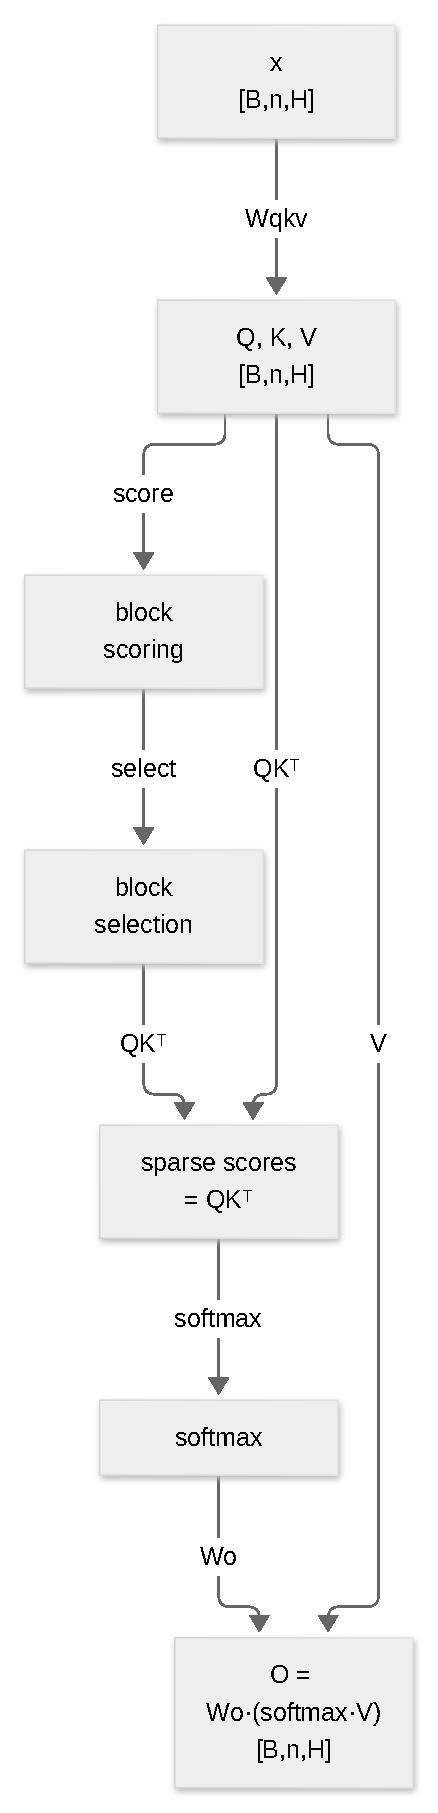
\includegraphics{../paper/figures/mixers/nsa.pdf}}
\caption{Flujo de datos de NSA: la puntuación y selección jerárquica de bloques restringen la matriz de puntuaciones a los bloques elegidos.}
\label{fig:mixer-nsa}
\end{figure}

\subsubsection{Formulación Matemática}

NSA \citep{yuan_nsa_2025} descompone la atención dispersa en tres ramas paralelas que se combinan mediante compuertas aprendidas.

\paragraph{Rama de compresión}: Un MLP aprendible $\varphi$ comprime bloques de clave-valor:

\[
\tilde{K}_t^{\text{cmp}} = \left[\varphi(k_{id+1:id+l})\right]_{\substack{1 \leq i \leq \lfloor(t-l)/d\rfloor}} \quad, \quad \tilde{V}_t^{\text{cmp}} = \left[\varphi(v_{id+1:id+l})\right]
\]

\paragraph{Rama de selección}: Los bloques de alta importancia se seleccionan basándose en puntajes comprimidos:

\[
p_t^{\text{cmp}} = \text{softmax}(q_t^\top \tilde{K}_t^{\text{cmp}} / \sqrt{d}), \quad I_t = \mathrm{TopK}(p_t^{\text{cmp}}, n), \quad \tilde{K}_t^{\text{sel}} = \mathrm{Recolectar}(K, I_t)
\]

\paragraph{Rama de ventana deslizante}: Contexto local fijo:

\[
\tilde{K}_t^{\text{win}} = K_{t-w:t}, \quad \tilde{V}_t^{\text{win}} = V_{t-w:t}
\]

\paragraph{Combinación con compuertas}: Las tres salidas de atención se combinan mediante compuertas aprendidas:

\[
\alpha_t^{(\text{cmp})} = \sigma(\text{Lineal}_\text{cmp}(q_t)), \quad \alpha_t^{(\text{sel})} = \sigma(\text{Lineal}_\text{sel}(q_t)), \quad \alpha_t^{(\text{win})} = \sigma(\text{Lineal}_\text{win}(q_t))
\]

\[
y_t = \alpha_t^{(\text{cmp})} \cdot \text{Attn}(q_t, \tilde{K}^{\text{cmp}}, \tilde{V}^{\text{cmp}}) + \alpha_t^{(\text{sel})} \cdot \text{Attn}(q_t, \tilde{K}^{\text{sel}}, \tilde{V}^{\text{sel}}) + \alpha_t^{(\text{win})} \cdot \text{Attn}(q_t, \tilde{K}^{\text{win}}, \tilde{V}^{\text{win}})
\]

\subsubsection{Pseudocódigo Algorítmico}

\begin{algorithm}[H]
\caption{NSA: Ramas Comprimida + Seleccionada + Ventana con Compuertas Aprendidas}
\begin{algorithmic}[1]
\Require Consulta $\mathbf{q}_t$, secuencias de Clave/Valor almacenadas en caché, tamaño de bloque $l$, stride $d$, conteo de selección $n$, ventana $w$
\Require MLP de compresión $\varphi$, redes de compuerta $\text{Lineal}_{\text{cmp}}, \text{Lineal}_{\text{sel}}, \text{Lineal}_{\text{win}}$
\Ensure Salida $\mathbf{y}_t$
\State \textbf{Rama de compresión:}
\For{$i = 1$ to $\lfloor t/d \rfloor$}
    \State $k_i^{\text{cmp}} \gets \varphi(\mathbf{K}_{id+1:id+l})$ \Comment{Comprimir bloque mediante MLP}
    \State $v_i^{\text{cmp}} \gets \varphi(\mathbf{V}_{id+1:id+l})$
\EndFor
\State $\tilde{\mathbf{K}}^{\text{cmp}} \gets [k_1^{\text{cmp}}, \ldots, k_{\lfloor t/d \rfloor}^{\text{cmp}}]$, $\tilde{\mathbf{V}}^{\text{cmp}} \gets [v_1^{\text{cmp}}, \ldots, v_{\lfloor t/d \rfloor}^{\text{cmp}}]$
\State $\mathbf{y}_t^{(\text{cmp})} \gets \text{SDPA}(\mathbf{q}_t, \tilde{\mathbf{K}}^{\text{cmp}}, \tilde{\mathbf{V}}^{\text{cmp}})$
\State \textbf{Rama de selección:}
\State Calcular puntajes sobre comprimidos: $\mathbf{s} \gets \text{softmax}(\mathbf{q}_t \tilde{\mathbf{K}}^{\text{cmp}\top} / \sqrt{d})$
\State Seleccionar los $n$ bloques más importantes: $I \gets \mathrm{TopK}(\mathbf{s}, n)$
\State Recolectar bloques completos: $\tilde{\mathbf{K}}^{\text{sel}} \gets [\mathbf{K}_{I_i d+1:I_i d+l}]_i$, $\tilde{\mathbf{V}}^{\text{sel}} \gets [\mathbf{V}_{I_i d+1:I_i d+l}]_i$
\State $\mathbf{y}_t^{(\text{sel})} \gets \text{SDPA}(\mathbf{q}_t, \tilde{\mathbf{K}}^{\text{sel}}, \tilde{\mathbf{V}}^{\text{sel}})$
\State \textbf{Rama de ventana:}
\State $\mathbf{y}_t^{(\text{win})} \gets \text{SDPA}(\mathbf{q}_t, \mathbf{K}_{t-w:t}, \mathbf{V}_{t-w:t})$
\State \textbf{Fusión con compuertas:}
\State $\alpha^{(\text{cmp})} \gets \sigma(\text{Lineal}_{\text{cmp}}(\mathbf{q}_t))$, $\alpha^{(\text{sel})} \gets \sigma(\text{Lineal}_{\text{sel}}(\mathbf{q}_t))$, $\alpha^{(\text{win})} \gets \sigma(\text{Lineal}_{\text{win}}(\mathbf{q}_t))$
\State $\mathbf{y}_t \gets \alpha^{(\text{cmp})} \mathbf{y}_t^{(\text{cmp})} + \alpha^{(\text{sel})} \mathbf{y}_t^{(\text{sel})} + \alpha^{(\text{win})} \mathbf{y}_t^{(\text{win})}$
\Return $\mathbf{y}_t$
\end{algorithmic}
\end{algorithm}

\subsubsection{Características Clave}

\begin{itemize}[leftmargin=*]
    \item \textbf{Complejidad}: $\mathcal{O}(t/d + n \cdot l + w)$ tokens atendidos por paso (significativamente reducido frente a $\mathcal{O}(t)$ para densa).
    \item \textbf{Entrenable}: Sí; entrenamiento directo con todas las ramas diferenciables.
    \item \textbf{Alineación con hardware}: Diseñado para utilización eficiente de núcleos tensoriales; la compresión y selección reducen la presión sobre el ancho de banda de memoria.
    \item \textbf{Fortaleza}: 11.6$\times$ de aceleración en decodificación y 9$\times$ de aceleración hacia adelante en secuencias de 64k; supera a la atención completa en muchas tareas.
    \item \textbf{Limitación}: Requiere kernels Triton/CUDA personalizados; la arquitectura multi-rama compleja aumenta la sobrecarga de ingeniería.
\end{itemize}

\subsection{FASA: Atención Dispersa Consciente de la Frecuencia}

\begin{figure}[H]
\centering
\fitfigure{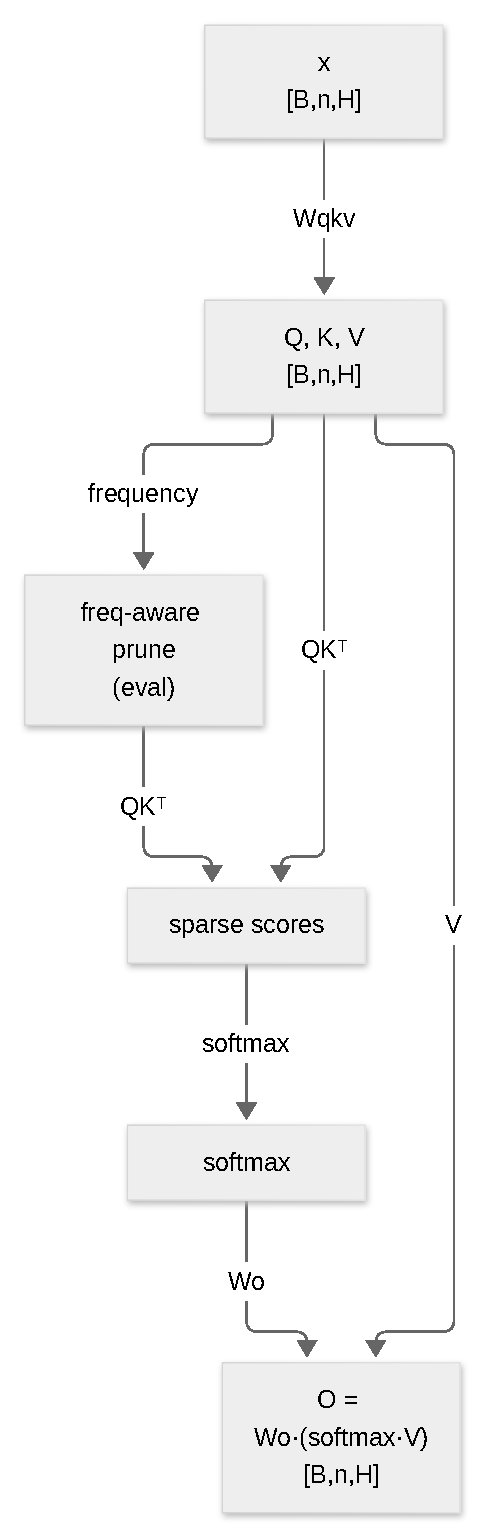
\includegraphics{../paper/figures/mixers/fasa.pdf}}
\caption{Flujo de datos de FASA: una etapa de poda sensible a la frecuencia (solo evaluación) descarta bloques de claves de bajo valor antes del softmax.}
\label{fig:mixer-fasa}
\end{figure}

\subsubsection{Formulación Matemática}

FASA \citep{wang_fasa_2026} es un \textbf{método en tiempo de inferencia sin entrenamiento} que explota la estructura del embedding de posición rotatorio (RoPE). Bajo RoPE, el embedding del token se rota por $\theta_i = B^{-2(i-1)/d}$, descomponiendo el espacio $d$-dimensional en $d/2$ fragmentos de frecuencia (FC).

\paragraph{Idea clave}: Solo un subconjunto pequeño ($ < 1\%$) de los FC importa para la conciencia contextual; la mayoría codifica patrones posicionales.

\paragraph{Identificación de fragmento de frecuencia dominante}: Para cada capa $l$ y cabeza $h$, identificar FC dominantes mediante concordancia contextual (CA):

\[
\text{CA}^{l,h,i} = \frac{|\text{TopK}(\alpha^{l,h}) \cap \text{TopK}(\alpha^{l,h,i})|}{K}
\]

donde $\alpha^{l,h}$ es la máscara de atención completa y $\alpha^{l,h,i}$ es la máscara usando solo el FC $i$. Los FC dominantes tienen CA alta---contribuyen significativamente al patrón de atención final.

\paragraph{Etapa de predicción de importancia de tokens (TIP)}: Usando solo FC dominantes, calcular importancia ligera por token:

\[
S_t^{l,h} = \sum_{i \in \mathcal{I}_{\text{dom}}^{l,h}} \alpha^{l,h,i}(\mathbf{q}_t, \mathbf{K}_{1:t}), \quad \mathcal{T}_t = \text{TopK-Índices}(S_t, N_{\text{fac}})
\]

\paragraph{Etapa de cálculo de atención enfocada (FAC)}: Calcular atención de precisión completa en los tokens seleccionados:

\[
\hat{\alpha}_{\text{FAC}} = \text{softmax}\left(\frac{\mathbf{q}_t \mathbf{K}_{\mathcal{T}_t}^\top}{\sqrt{d}}\right), \quad \mathbf{o}_t = \hat{\alpha}_{\text{FAC}} \mathbf{V}_{\mathcal{T}_t}
\]

\subsubsection{Pseudocódigo Algorítmico}

\begin{algorithm}[H]
\caption{FASA: Atención Dispersa Consciente de la Frecuencia (en Tiempo de Inferencia)}
\begin{algorithmic}[1]
\Require Consulta actual $\mathbf{q}_t$, Clave/Valor almacenados en caché $\mathbf{K}_{1:t}, \mathbf{V}_{1:t}$, base RoPE $B$, FC dominantes $\mathcal{I}_{\text{dom}}$
\Require Presupuesto TIP $N_{\text{tip}}$, presupuesto FAC $N_{\text{fac}}$
\Ensure Salida $\mathbf{o}_t$
\State \textbf{Etapa 1: Predicción de Importancia de Tokens (TIP)}
\For{capa $l$ y cabeza $h$}
    \For{posición $i = 1$ to $t$}
        \State Calcular importancia desde FC dominantes: $s_i \gets 0$
        \For{$fc \in \mathcal{I}_{\text{dom}}^{l,h}$}
            \State Rotar consulta y clave en FC $fc$: $\mathbf{q}^{(fc)}, \mathbf{k}_i^{(fc)}$
            \State $s_i^{(fc)} \gets \text{softmax}(\mathbf{q}^{(fc)} \mathbf{k}_i^{(fc)\top} / \sqrt{d}) $
            \State $s_i \gets s_i + s_i^{(fc)}$
        \EndFor
    \EndFor
    \State $\mathcal{T}_t \gets \mathrm{TopK}\text{-Índices}([s_1, \ldots, s_t], N_{\text{fac}})$ \Comment{Seleccionar tokens principales}
\EndFor
\State \textbf{Etapa 2: Cálculo de Atención Enfocada (FAC)}
\State $\text{puntajes}_{\text{fac}} \gets \mathbf{q}_t \mathbf{K}_{\mathcal{T}_t}^\top / \sqrt{d}$ \Comment{Producto punto de precisión completa}
\State $\alpha_{\text{fac}} \gets \text{softmax}(\text{puntajes}_{\text{fac}})$ \Comment{Softmax completo}
\State $\mathbf{o}_t \gets \alpha_{\text{fac}} \mathbf{V}_{\mathcal{T}_t}$ \Comment{Suma ponderada de valores}
\Return $\mathbf{o}_t$
\end{algorithmic}
\end{algorithm}

\subsubsection{Características Clave}

\begin{itemize}[leftmargin=*]
    \item \textbf{Complejidad}: TIP es $\mathcal{O}(t \cdot N_{\text{tip}})$; FAC es $\mathcal{O}(N_{\text{fac}} \cdot d)$.
    \item \textbf{Entrenable}: No; optimización de inferencia sin entrenamiento.
    \item \textbf{Aplicabilidad}: Requiere modelos basados en RoPE; extendido a ALiBi y MLA con modificaciones.
    \item \textbf{Fortaleza}: Precisión cercana a la óptima con $\leq 256$ tokens de entre millones; hasta 2.56$\times$ de aceleración en decodificación; ortogonal a la cuantización.
    \item \textbf{Limitación}: Requiere calibración fuera de línea; la identificación de FC dominantes añade sobrecarga de preprocesamiento.
\end{itemize}

\paragraph{Nota de implementación (entrenamiento vs.\ inferencia).} En este repositorio la ruta dispersa TIP/FAC es solo de inferencia. Mientras el modelo está en modo entrenamiento, la capa híbrida contenedora sustituye atención estándar densa sobre las mismas proyecciones $\mathbf{q}/\mathbf{k}/\mathbf{v}/\mathbf{o}$, de modo que el mixer puede entrenarse desde cero y los pesos optimizados durante el entrenamiento son exactamente los que lee la ruta dispersa en evaluación.

\subsection{SpargeAttn: Filtrado de Dos Etapas a Nivel de Bloques}

\begin{figure}[H]
\centering
\fitfigure{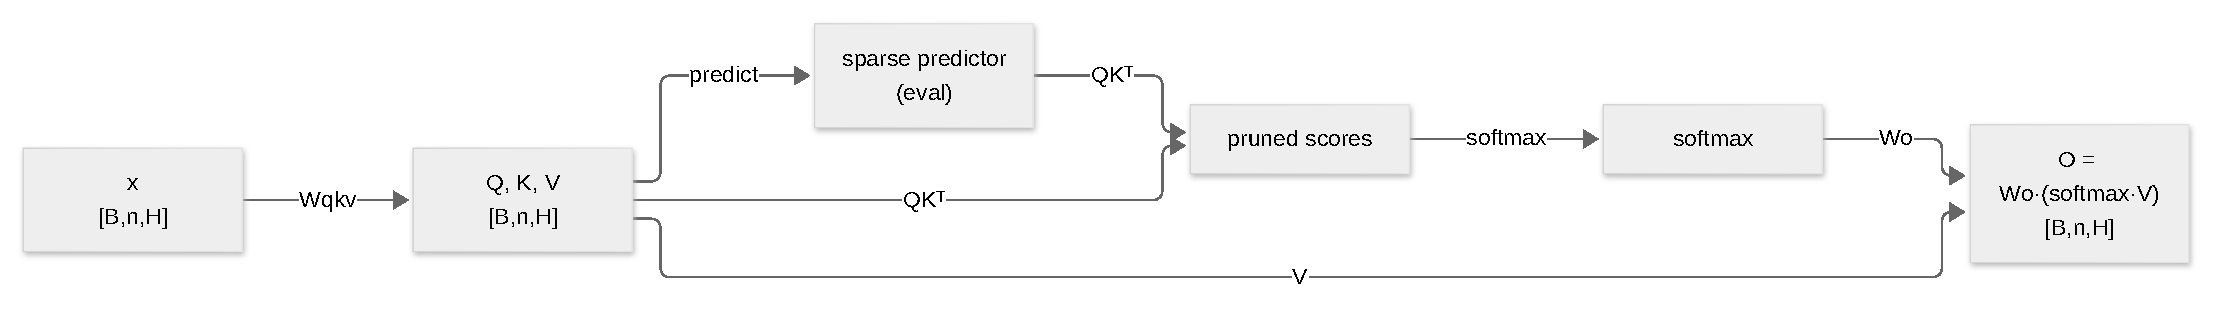
\includegraphics{../paper/figures/mixers/sparge.pdf}}
\caption{Flujo de datos de SpargeAttn: un predictor disperso (solo evaluación) poda bloques de claves antes del softmax.}
\label{fig:mixer-sparge}
\end{figure}

\subsubsection{Formulación Matemática}

SpargeAttn \citep{zhang_spargeattn_2025} es un \textbf{método universal sin entrenamiento} que predice qué bloques de la matriz de atención contendrán valores insignificantes y omite el cálculo para esos bloques.

\paragraph{Etapa 1 --- Predicción dispersa}: Calcular importancia proxy de bajo costo $\hat{s}_{ij}$ para el bloque $(i,j)$:

\[
\hat{s}_{ij} = f_{\text{pred}}(\mathbf{Q}_i, \mathbf{K}_j; \text{hiperparámetros}), \quad \text{omitir si } \hat{s}_{ij} < \epsilon_1
\]

Los predictores comunes incluyen similitud de media de bloque o estadísticas de autosimilitud.

\paragraph{Etapa 2 --- Filtrado consciente de softmax}: Después de calcular $\tilde{P}_{ij} = \text{softmax}(Q_i K_j^\top/\sqrt{d})$, verificar si la probabilidad máxima del bloque es insignificante en relación con el máximo de softmax en ejecución:

\[
\text{omitir } P_{ij} V_j \quad \text{si} \quad \max(\tilde{P}_{ij}) < e^{m_{\text{antiguo}} - m_{\text{nuevo}}} \cdot \epsilon_2
\]

donde $m_{\text{antiguo}}, m_{\text{nuevo}}$ son máximos del softmax en línea en ejecución (calculados mediante numéricos estilo FlashAttention).

\subsubsection{Pseudocódigo Algorítmico}

\begin{algorithm}[H]
\caption{SpargeAttn: Filtrado Disperso de Dos Etapas por Bloques}
\begin{algorithmic}[1]
\Require Bloques de consulta $\mathbf{Q}_i$ para $i = 1, \ldots, n_b$, Bloques de clave $\mathbf{K}_j$ para $j = 1, \ldots, n_b$, Bloques de valor $\mathbf{V}_j$
\Require Umbral de predicción $\epsilon_1$, umbral de softmax $\epsilon_2$, tamaño de bloque $b_s$
\Ensure Salida $\mathbf{Y}$
\State Inicializar: máximo de softmax en línea $m_{\text{global}} \gets -\infty$
\For{fila de bloque $i = 1$ to $n_b$}
    \State Inicializar: salida de fila de bloque $\mathbf{Y}_i \gets 0$, máximo local $m_i \gets -\infty$
    \For{columna de bloque $j = 1$ to $n_b$}
        \State \textbf{Etapa 1: Predicción Dispersa}
        \State Calcular importancia proxy: $\hat{s}_{ij} \gets f_{\text{pred}}(\mathbf{Q}_i, \mathbf{K}_j)$
        \If{$\hat{s}_{ij} < \epsilon_1$}
            \State \textbf{omitir} este bloque $[i,j]$  \Comment{Terminación temprana}
            \State \textbf{continuar} \Comment{Pasar al siguiente bloque}
        \EndIf
        \State \textbf{Etapa 2: Calcular y Filtrar}
        \State $\tilde{P}_{ij} \gets \text{softmax}(\mathbf{Q}_i \mathbf{K}_j^\top / \sqrt{d})$
        \State $m_{\text{bloque}} \gets \max(\tilde{P}_{ij})$
        \If{$m_{\text{bloque}} < e^{m_i - m_{\text{global}}} \cdot \epsilon_2$}
            \State El bloque contribuye insignificantemente; omitir  \Comment{Poda consciente de softmax}
            \State \textbf{continuar}
        \EndIf
        \State Actualizar máximo global: $m_i \gets \max(m_i, m_{\text{bloque}})$
        \State Acumular: $\mathbf{Y}_i \gets \mathbf{Y}_i + \tilde{P}_{ij} \mathbf{V}_j$
    \EndFor
    \State $m_{\text{global}} \gets \max(m_{\text{global}}, m_i)$
\EndFor
\Return $\mathbf{Y}$
\end{algorithmic}
\end{algorithm}

\subsubsection{Características Clave}

\begin{itemize}[leftmargin=*]
    \item \textbf{Complejidad}: Empírica $\mathcal{O}(n^2 \cdot s)$ donde $s$ es la fracción de bloques no omitidos (típicamente 0.2--0.5).
    \item \textbf{Entrenable}: No; aceleración plug-and-play para modelos existentes.
    \item \textbf{Universalidad}: Funciona en modelos de lenguaje, modelos de difusión de imágenes y generación de video.
    \item \textbf{Fortaleza}: 2.5--5$\times$ de aceleración comparado con métodos densos o dispersos anteriores; compatible con cuantización (integración SageAttention).
    \item \textbf{Limitación}: La aceleración depende de la dispersidad inherente; la granularidad a nivel de bloque puede pasar por alto patrones más finos; se requiere ajuste de umbral por familia de modelos.
\end{itemize}

\paragraph{Nota de implementación (entrenamiento vs.\ inferencia).} En este repositorio el filtro de bloques en dos etapas es solo de inferencia. Mientras el modelo está en modo entrenamiento, la capa híbrida contenedora sustituye atención estándar densa sobre las mismas proyecciones $\mathbf{q}/\mathbf{k}/\mathbf{v}/\mathbf{o}$, de modo que el mixer puede entrenarse desde cero y los pesos optimizados durante el entrenamiento son exactamente los que lee la ruta dispersa en evaluación.

\subsection{MSA (MiniMax Sparse Attention): Atención Dispersa por Bloques con Rama de Índice Ligera}

\begin{figure}[H]
\centering
\fitfigure{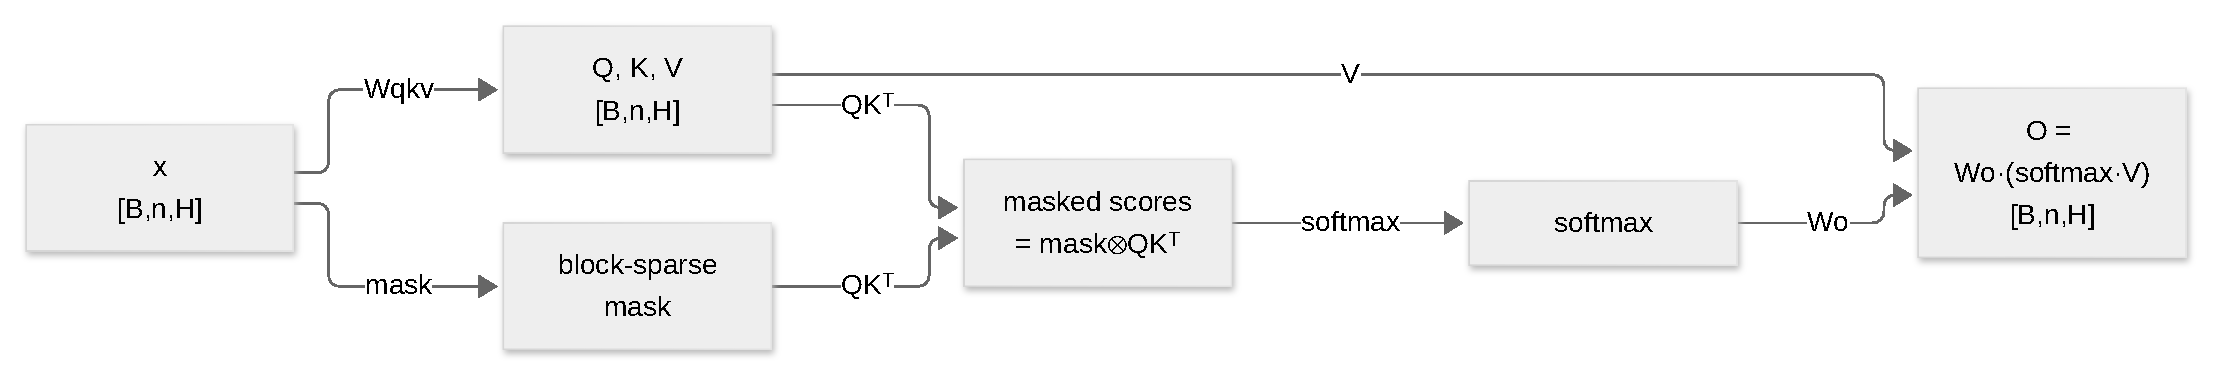
\includegraphics{../paper/figures/mixers/msa.pdf}}
\caption{Flujo de datos de MSA: una máscara de bloques dispersos restringe la matriz de puntuaciones antes del softmax.}
\label{fig:mixer-msa}
\end{figure}

\subsubsection{Formulación Matemática}

MSA \citep{lai_minimax_2026} es un mecanismo de atención dispersa por bloques construido sobre atención agrupada por consultas (GQA) que combina una \textbf{Rama de Índice} ligera para la selección de bloques con una \textbf{Rama Principal} para atención softmax dispersa por bloques exacta sobre los bloques seleccionados. Sea $N$ la longitud de la secuencia, $B_k = 128$ el tamaño de bloque, y $k = 16$ el número de bloques seleccionados por consulta (lo que yield un presupuesto fijo por consulta de $k \cdot B_k = 2048$ tokens independientemente de $N$).

\paragraph{Rama de Índice}: Una proyección de baja dimensionalidad produce consultas de índice $\mathbf{q}_t^{\text{idx}} \in \mathbb{R}^{d_{\text{idx}}}$ y representantes de bloque $\mathbf{r}_b \in \mathbb{R}^{d_{\text{idx}}}$ para cada bloque KV $b$. Los puntajes de índice por grupo GQA son:
\[
s_{t,b}^{(g)} = \mathbf{q}_t^{\text{idx},(g)} \cdot \mathbf{r}_b, \qquad \mathcal{I}_t^{(g)} = \mathrm{TopK}\left(\{s_{t,b}^{(g)}\}_{b=1}^{N/B_k},\; k\right)
\]
La entrada del índice está \textbf{desconectada} (stop-gradient), de modo que los gradientes no fluyen hacia atrás a través de la entrada del indexador; la Rama de Índice se entrena en su lugar mediante una pérdida de alineación KL entre su distribución de atención y la distribución de la Rama Principal. Debido a que softmax preserva el orden, los puntajes crudos de índice se alimentan directamente al operador top-$k$ \emph{sin} un softmax explícito (\textbf{top-$k$ sin exponencial}), reduciendo el costo numérico.

\paragraph{Bloque local forzado}: El bloque que contiene la posición de consulta $t$ \textbf{siempre} se incluye en $\mathcal{I}_t^{(g)}$, garantizando cobertura de contexto local.

\paragraph{Rama Principal}: La atención estándar de producto punto escalado se calcula exactamente sobre la unión de los bloques seleccionados:
\[
\mathbf{o}_t^{(h)} = \mathrm{softmax}\left(\frac{\mathbf{q}_t^{(h)} \mathbf{K}_{\mathcal{I}_t}^{(h)\top}}{\sqrt{d_h}}\right) \mathbf{V}_{\mathcal{I}_t}^{(h)}
\]
donde $\mathbf{K}_{\mathcal{I}_t}, \mathbf{V}_{\mathcal{I}_t}$ reúnen los tensores de clave/valor de precisión completa de los bloques seleccionados. La selección se realiza independientemente por grupo GQA, de modo que diferentes grupos de consulta dentro de la misma capa pueden atender a diferentes subconjuntos de bloques.

\subsubsection{Pseudocódigo Algorítmico}

\begin{algorithm}[H]
\caption{MSA: Atención Dispersa MiniMax con Ramas de Índice + Principal}
\begin{algorithmic}[1]
\Require Consulta $\mathbf{Q} \in \mathbb{R}^{N \times d}$, Clave $\mathbf{K}$, Valor $\mathbf{V}$, tamaño de bloque $B_k = 128$, bloques top-$k$ $k = 16$
\Require Proyección de índice $W_{\text{idx}}$ (entrada desconectada), representantes de bloque $\{\mathbf{r}_b\}$
\Ensure Salida $\mathbf{Y} \in \mathbb{R}^{N \times d}$
\State Calcular representantes de bloque: $\mathbf{r}_b \gets \mathrm{mean}(\mathbf{K}_{bB_k:(b+1)B_k})$ para $b = 1, \ldots, N/B_k$
\For{posición de consulta $t = 1, \ldots, N$}
    \For{cada grupo GQA $g$}
        \State $\mathbf{q}_t^{\text{idx}} \gets \mathrm{sg}(W_{\text{idx}} \mathbf{x}_t)$ \Comment{consulta de índice desconectada}
        \State Calcular puntajes de bloque: $s_b \gets \mathbf{q}_t^{\text{idx}} \cdot \mathbf{r}_b$
        \State Identificar bloque local: $b_{\text{local}} \gets \lfloor t / B_k \rfloor$
        \State $\mathcal{I}_t^{(g)} \gets \mathrm{TopK}(\{s_b\}, k) \cup \{b_{\text{local}}\}$ \Comment{top-$k$ sin exp + local forzado}
    \EndFor
    \State Reunir KV seleccionado: $\tilde{\mathbf{K}}_t \gets \mathrm{Gather}(\mathbf{K}, \mathcal{I}_t)$, $\tilde{\mathbf{V}}_t \gets \mathrm{Gather}(\mathbf{V}, \mathcal{I}_t)$
    \State Rama principal SDPA: $\mathbf{y}_t \gets \mathrm{softmax}(\mathbf{q}_t \tilde{\mathbf{K}}_t^\top / \sqrt{d_h}) \tilde{\mathbf{V}}_t$
\EndFor
\State Agregar pérdida de alineación KL $\mathcal{L}_{\text{KL}} = \mathrm{KL}(\text{dist índice} \,\|\, \text{dist principal})$ durante el entrenamiento
\Return $\mathbf{Y}$
\end{algorithmic}
\end{algorithm}

\subsubsection{Características Clave}

\begin{itemize}[leftmargin=*]
    \item \textbf{Complejidad}: Rama de índice $\mathcal{O}(H_{\text{kv}} \cdot d_{\text{idx}} \cdot N^2)$; Rama principal $\mathcal{O}(H_q \cdot d_h \cdot N \cdot k \cdot B_k)$. Presupuesto por consulta fijo en $k \cdot B_k = 2048$ tokens independientemente de $N$.
    \item \textbf{Entrenable}: Sí; de extremo a extremo (la Rama de Índice se entrena mediante una pérdida de alineación KL, no es solo inferencia).
    \item \textbf{Estado}: Caché KV $\mathcal{O}(N)$ (tamaño GQA); sin expansión de la dimensión de estado recurrente.
    \item \textbf{Fortaleza}: Desplegado en el modelo 109B MiniMax-M3, MSA logra una reducción de cómputo de atención por token de $28.4\times$ a contexto de 1M, con $14.2\times$ en prefill y $7.6\times$ en decodificación en GPUs H800.
    \item \textbf{Limitación}: La granularidad de selección es fija a nivel de bloque ($B_k = 128$); el bloque local forzado y la selección independiente por grupo aumentan la complejidad de ingeniería y requieren kernels personalizados de bloques dispersos.
\end{itemize}

\subsection{SparDA (Atención Dispersa Desacoplada): Selección de Bloques Anticipada Guiada por Pronóstico}

\begin{figure}[H]
\centering
\fitfigure{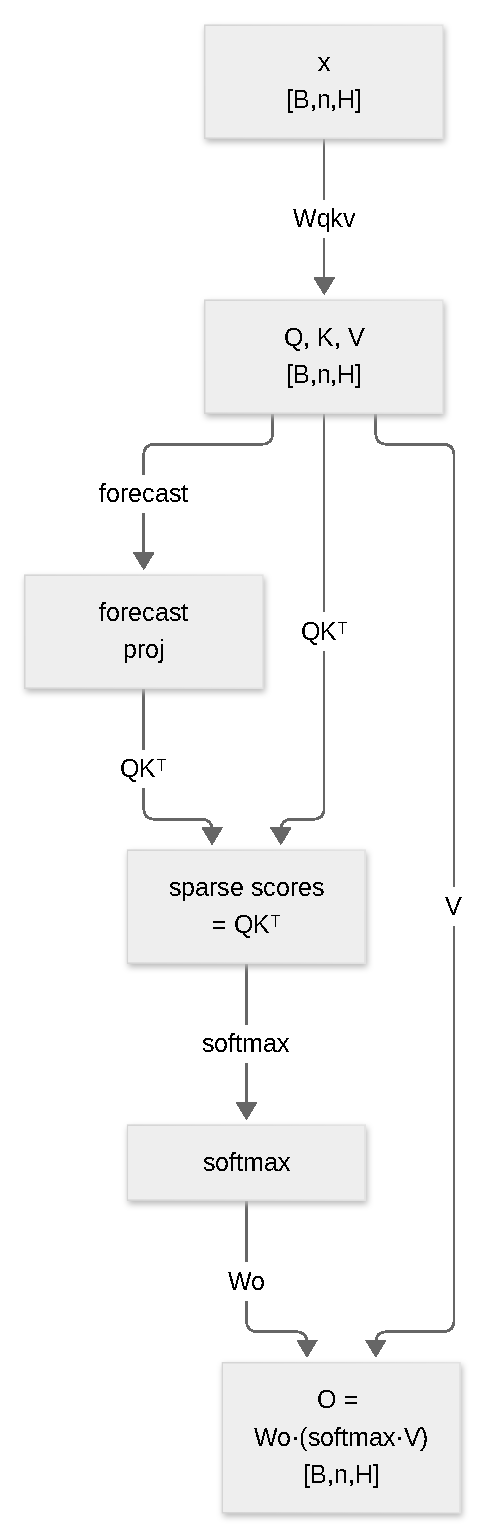
\includegraphics{../paper/figures/mixers/sparda.pdf}}
\caption{Flujo de datos de SparDA: una proyección de pronóstico guía la selección anticipada de bloques antes del softmax.}
\label{fig:mixer-sparda}
\end{figure}

\subsubsection{Formulación Matemática}

SparDA \citep{fu_sparda_2026} introduce un esquema de atención dispersa \textbf{desacoplado} que aumenta las proyecciones estándar por capa $Q, K, V$ con una cuarta proyección, el \textbf{Pronóstico}, que predice los bloques KV que serán necesarios en la \emph{siguiente} capa. Esta anticipación permite solapar el prefetch CPU-a-GPU de los bloques seleccionados de la siguiente capa con la ejecución de la capa actual, ocultando la latencia de offload que afecta a las implementaciones de atención dispersa en hardware con memoria limitada.

\paragraph{Proyección de Pronóstico}: Para la entrada $\mathbf{x} \in \mathbb{R}^{N \times d}$,
\[
\mathbf{F} = \mathbf{x} \mathbf{W}_F \in \mathbb{R}^{N \times H_{\text{kv}} \times d_f}
\]
con \textbf{una cabeza de Pronóstico por grupo GQA}, lo que reduce la sobrecarga de selección frente a los selectores multi-cabeza usados en trabajos anteriores.

\paragraph{Puntuación y selección de bloques}: Para cada consulta $i$ y bloque KV $b$ con representante $\mathbf{r}_b$:
\[
S_{i,b} = \mathbf{F}_i \cdot \mathbf{r}_b, \qquad \mathcal{I}_i = \mathrm{TopK}(\{S_{i,b}\}_b, k)
\]
\paragraph{Atención dispersa por bloques}: La atención estándar de producto punto escalado se calcula entonces sobre los bloques seleccionados:
\[
\mathbf{o}_i = \mathrm{softmax}\left(\frac{\mathbf{q}_i \mathbf{K}_{\mathcal{I}_i}^\top}{\sqrt{d_h}}\right) \mathbf{V}_{\mathcal{I}_i}
\]
\paragraph{Entrenamiento}: SparDA añade menos del $0.5\%$ de parámetros adicionales. Solo las proyecciones de Pronóstico se entrenan, emparejando la distribución de atención del selector disperso original (congelado)---una destilación ligera que preserva el comportamiento del modelo base mientras habilita el prefetch anticipado.

\subsubsection{Pseudocódigo Algorítmico}

\begin{algorithm}[H]
\caption{SparDA: Atención Dispersa Desacoplada con Prefetch de Pronóstico}
\begin{algorithmic}[1]
\Require Entrada $\mathbf{x} \in \mathbb{R}^{N \times d}$, bloques de Clave/Valor en caché, bloques top-$k$ $k$
\Require Proyecciones $W_q, W_k, W_v, W_F$; selector base congelado $\pi_{\text{orig}}$
\Ensure Salida $\mathbf{Y}$; bloques prefetched para la siguiente capa
\State Calcular Pronóstico: $\mathbf{F} \gets \mathbf{x} \mathbf{W}_F$ \Comment{una cabeza por grupo GQA}
\For{consulta $i = 1, \ldots, N$}
    \State Calcular puntajes de bloque: $S_{i,b} \gets \mathbf{F}_i \cdot \mathbf{r}_b$ para cada bloque $b$
    \State Seleccionar: $\mathcal{I}_i \gets \mathrm{TopK}(\{S_{i,b}\}, k)$
    \State \textbf{Prefetch} $\mathbf{K}_{\mathcal{I}_i}, \mathbf{V}_{\mathcal{I}_i}$ de CPU a GPU para la \emph{siguiente} capa \Comment{solapa con la capa actual}
\EndFor
\State Calcular SDPA dispersa por bloques sobre los bloques seleccionados de la capa actual: $\mathbf{Y} \gets \mathrm{BlockSparseSDPA}(\mathbf{Q}, \mathbf{K}, \mathbf{V}, \{\mathcal{I}_i\})$
\State Pérdida de entrenamiento: $\mathcal{L} \gets \mathrm{KL}(\text{dist Pronóstico} \,\|\, \pi_{\text{orig}})$ \Comment{solo se actualiza $W_F$}
\Return $\mathbf{Y}$
\end{algorithmic}
\end{algorithm}

\subsubsection{Características Clave}

\begin{itemize}[leftmargin=*]
    \item \textbf{Complejidad}: Pronóstico $\mathcal{O}(H_{\text{kv}} \cdot d_f \cdot N \cdot N_{\text{bloques}})$; Atención principal $\mathcal{O}(H_q \cdot d_h \cdot N \cdot k \cdot B_k)$.
    \item \textbf{Entrenable}: Sí; solo las proyecciones de Pronóstico se entrenan ($<0.5\%$ parámetros extra).
    \item \textbf{Fortaleza}: En dos modelos sparse-pretrained de 8B, SparDA logra hasta $1.25\times$ en prefill y $1.7\times$ en decodificación sobre el baseline de offload de atención dispersa, y hasta $5.3\times$ throughput de decodificación frente a un baseline disperso sin offload.
    \item \textbf{Limitación}: Requiere un pipeline de offload CPU--GPU y un selector base congelado; el beneficio anticipado depende de que la demanda de bloques de la siguiente capa sea predecible a partir del Pronóstico actual.
\end{itemize}

\subsection{Espacio de Diseño y Criterios de Selección}

Los diez métodos de atención dispersa ocupan posiciones complementarias en un espacio de diseño multidimensional:

\begin{itemize}[leftmargin=*]
    \item \textbf{Patrones geométricos/fijos} (Sparse Transformer, Longformer): Simples de implementar y analizar, pero los patrones no se adaptan al contenido.
    \item \textbf{Desalojo de KV con memoria fija} (SWA con sumideros): La política más barata posible---conservar un prefijo sumidero y una ventana reciente, descartar el resto. Sin parámetros extra, sin entrenamiento, memoria acotada.
    \item \textbf{Selección aprendida} (SparseK, NSA): Permiten adaptación mediante redes de selección entrenables, a costa de mayor complejidad de implementación.
    \item \textbf{Aceleración sin entrenamiento} (FASA, SpargeAttn): Permiten aceleración directa de modelos existentes sin reentrenamiento, adecuados para sistemas desplegados.
    \item \textbf{Garantías teóricas} (BigBird): Proporcionan demostraciones formales de completitud expresiva, importantes para comprender los márgenes de seguridad.
\end{itemize}

\textbf{Orientación de selección:}
\begin{enumerate}[leftmargin=*]
    \item \textbf{Entrenamiento de nuevos modelos} donde los recursos lo permitan: NSA o SparseK para máxima aceleración de inferencia; BigBird para garantía teórica; SWA con sumideros como el baseline de bajo costo más fuerte.
    \item \textbf{Comprensión de documentos de contexto largo}: SWA con sumideros (ventana 256--512) para la mejor precisión por byte de caché KV; Longformer o FASA por simplicidad práctica; NSA para escala extrema.
    \item \textbf{Aceleración de modelos existentes}: SWA con sumideros como baseline sin entrenamiento por defecto (superó a la mayoría de los retrofits de atención lineal en el estudio original); FASA para LLMs basados en RoPE; SpargeAttn para cualquier arquitectura.
    \item \textbf{Entornos con recursos limitados}: SWA con sumideros para un presupuesto de memoria fijo; Sparse Transformer por simplicidad y eficiencia probada a escala moderada.
\end{enumerate}


\section{Familias de Atención con Compuerta---Análisis Exhaustivo de Literatura}
\label{sec:annex-gated}

\subsection{Resumen Ejecutivo: Compuertas para el Control de Memoria}

El campo emergente de los \emph{mecanismos de atención con compuerta} aborda un desafío fundamental en el modelado de secuencias: ¿cómo debe retenerse, olvidarse y actualizarse la información a medida que el modelo procesa nuevos tokens? Los estados recurrentes aditivos tradicionales acumulan toda la información sin borrado, lo que lleva a la saturación de memoria y a la incapacidad de adaptarse a contextos cambiantes. La atención softmax proporciona expresividad completa pero usa un caché KV de $\mathcal{O}(Ld)$ durante la inferencia, limitando el tamaño de la ventana de contexto. Los mecanismos con compuerta proporcionan un punto intermedio: control selectivo sobre la supervivencia de la información.

El principio unificador entre las arquitecturas con compuerta es que las compuertas controlan \textit{qué información sobrevive}. Las compuertas operan en tres niveles distintos:
\begin{enumerate}[leftmargin=*]
    \item \textbf{Decaimiento del estado recurrente} (GLA, HGRN2): Compuertas multiplicativas sobre la matriz de memoria $S_t$ controlan cuánto del estado anterior persiste en el siguiente paso.
    \item \textbf{Intensidad de escritura en actualizaciones recurrentes} (DeltaNet, Gated DeltaNet, Gated DeltaNet-2): Las compuertas controlan la magnitud y la dirección canalizada de la nueva información escrita en la memoria.
    \item \textbf{Sesgo de logits softmax} (FoX): Las compuertas inyectan sesgo de actualidad a nivel de token en el cálculo de logits de atención.
    \item \textbf{Dispersidad post-atención} (Gated Softmax): Las compuertas escalan selectivamente los canales de salida de SDPA.
\end{enumerate}

Este apéndice sintetiza ocho arquitecturas principales de atención con compuerta publicadas entre 2023 y 2026, analizando sus fundamentos matemáticos, características de eficiencia en hardware y compensaciones empíricas.

\subsection{1. Atención Lineal con Compuerta (GLA)}

\begin{figure}[H]
\centering
\fitfigure{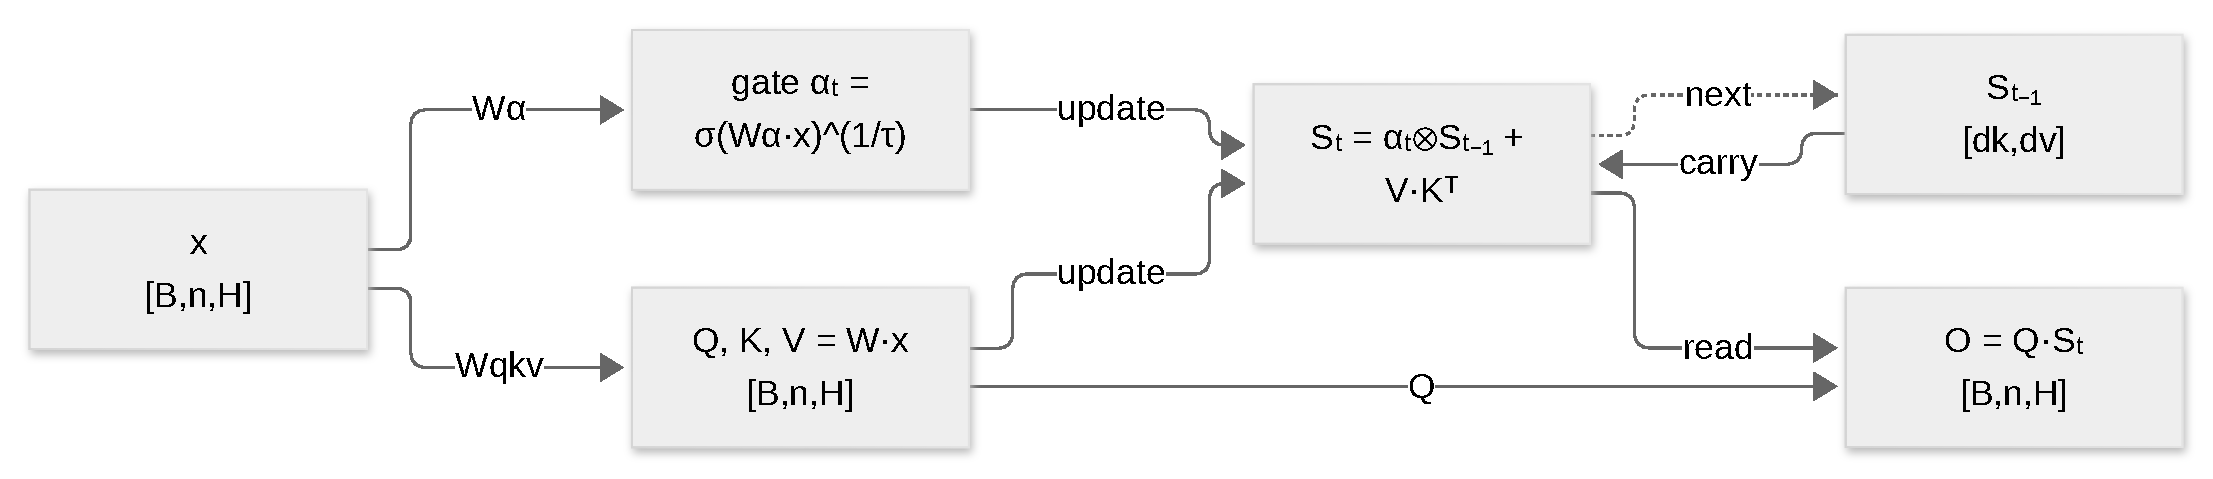
\includegraphics{../paper/figures/mixers/gla.pdf}}
\caption{Flujo de datos de GLA: una compuerta sigmoide decae el estado recurrente antes de sumar el producto externo clave/valor.}
\label{fig:mixer-gla}
\end{figure}

\subsubsection{Fundamento Matemático}

La Atención Lineal con Compuerta \citep{yang_gla_2023} aumenta la atención lineal estándar (que usa un estado recurrente con valor de matriz) con decaimiento multiplicativo dependiente de los datos. La atención lineal estándar reformula el mecanismo softmax tradicional como una recurrencia sobre estados ocultos:
\[
\mathbf{S}_t = \mathbf{S}_{t-1} + \mathbf{v}_t \mathbf{k}_t^\top, \quad \mathbf{o}_t = \mathbf{S}_t \mathbf{q}_t
\]
donde el estado $\mathbf{S}_t \in \mathbb{R}^{d_v \times d_k}$ acumula productos externos. Esta formulación puramente aditiva sufre de ``sobrecarga de memoria'': la información se acumula monótonamente y no puede borrarse, degradando el rendimiento en tareas que requieren selección de contexto.

GLA introduce una \textbf{matriz de compuerta diagonal} $\mathbf{G}_t \in [0,1]^{d_k \times d_k}$ dependiente de los datos:
\[
\mathbf{S}_t = \mathbf{G}_t \odot \mathbf{S}_{t-1} + \mathbf{v}_t \mathbf{k}_t^\top, \quad \mathbf{o}_t = \mathbf{S}_t \mathbf{q}_t
\]
La compuerta $\mathbf{G}_t$ se parametriza con una estructura de producto externo:
\[
\mathbf{G}_t = \mathbf{1} \boldsymbol{\alpha}_t^\top, \quad \boldsymbol{\alpha}_t = \text{logsigmoid}\left(\mathbf{W}_{gk} \mathbf{x}_t\right) / c
\]
donde $\mathbf{W}_{gk}$ es una proyección de rango bajo ($\mathbb{R}^{d \to d_k}$) y $c \approx 16$ es un normalizador. La activación logsigmoid mapea $\alpha_t \in \mathbb{R}$ a aproximadamente $[-1/2, 0]$, y la división por $c$ contrae esto aún más para que esté cerca de la identidad en la inicialización. La compuerta resultante $G_t = 1 + \alpha_t \approx 1$ cerca de la inicialización, luego aprende a decaer $(\alpha_t \to -\infty)$ información histórica.

\begin{algorithm}[H]
\caption{Atención Lineal con Compuerta (Forma Recurrente)}
\begin{algorithmic}[1]
\Require Entrada $\mathbf{x}_t$; estado anterior $\mathbf{S}_{t-1}$
\Require Proyecciones: $W_q, W_k, W_v$ (estándar); $W_{gk}$ (proyección de compuerta)
\Ensure Salida $\mathbf{o}_t$ y estado actualizado $\mathbf{S}_t$
\State $\mathbf{q}_t \gets W_q \mathbf{x}_t$
\State $\mathbf{k}_t \gets W_k \mathbf{x}_t$
\State $\mathbf{v}_t \gets W_v \mathbf{x}_t$
\State Calcular compuerta: $\boldsymbol{\alpha}_t \gets \text{logsigmoid}(W_{gk} \mathbf{x}_t) / 16$ \Comment{Decaimiento por dimensión de clave}
\State Aplicar compuerta de producto externo: $\mathbf{G}_t \gets \mathbf{1} \boldsymbol{\alpha}_t^\top$  \Comment{producto externo diagonal}
\State Decaer estado anterior: $\mathbf{S}_t^\text{decaimiento} \gets \mathbf{G}_t \odot \mathbf{S}_{t-1}$ \Comment{producto elemento a elemento}
\State Agregar nueva asociación: $\mathbf{S}_t \gets \mathbf{S}_t^\text{decaimiento} + \mathbf{v}_t \mathbf{k}_t^\top$
\State Recuperar mediante consulta: $\mathbf{o}_t^\text{crudo} \gets \mathbf{S}_t \mathbf{q}_t$
\State Aplicar compuerta de salida: $\mathbf{o}_t \gets \text{GroupNorm}(\mathbf{o}_t^\text{crudo}) \otimes \text{SiLU}(W_g \mathbf{x}_t)$
\Return $\mathbf{o}_t$, $\mathbf{S}_t$
\end{algorithmic}
\end{algorithm}

\subsubsection{Entrenamiento Eficiente en Hardware}

Para el entrenamiento paralelo, GLA usa un algoritmo por fragmentos que agrupa tokens en fragmentos $C$ y calcula transiciones recurrentes en paralelo:
\[
\mathbf{O}_{[t]} = \overleftarrow{\mathbf{Q}}_{[t]} \mathbf{S}_{[t]}^\top + \left(\mathbf{Q}_{[t]} \mathbf{K}_{[t]}^\top \odot \mathbf{\Gamma}_{[t]}\right) \mathbf{V}_{[t]}
\]
donde $\overleftarrow{\mathbf{Q}}_{[t]}$ atiende al estado en el límite del fragmento (retrospectiva), y $\mathbf{\Gamma}_{[t]}$ es la máscara causal con escalado consciente del decaimiento:
\[
\mathbf{\Gamma}_{[t],ij} = \begin{cases} \prod_{l=j}^{i-1} \alpha_l & \text{si } i > j \text{ (retrospectiva)} \\ \prod_{l=1}^{i-j} \alpha_l & \text{si } i \le j \text{ (en-fragmento)} \end{cases}
\]
Este diseño maximiza las operaciones matmul susceptibles de aceleración mediante núcleos tensoriales, logrando una complejidad total subcuadrática $\mathcal{O}(nLd^2/C)$ donde $L$ es el número de cabezas de atención y $C$ es el tamaño del fragmento.

\subsubsection{Fortalezas y Limitaciones}

\begin{table}[H]
\centering
\small
\begin{tabularx}{0.95\linewidth}{Xp{4cm}p{4cm}}
\toprule
\textbf{Aspecto} & \textbf{Fortalezas} & \textbf{Limitaciones} \\
\midrule
Eficiencia computacional & Entrenamiento subcuadrático mediante paralelismo por fragmentos. Inferencia con memoria constante $O(d^2)$. & Requiere kernels CUDA/Triton personalizados; no disponible en todos los frameworks. \\
Generalización de contexto & Extiende entrenamiento de 2K tokens a más de 20K tokens con degradación de perplejidad insignificante. & Aún rinde por debajo de softmax en benchmarks con mucha recuperación (aguja en el pajar). \\
Selectividad & Decaimiento dependiente de los datos por dimensión de clave. & La estructura de compuerta limita la selectividad por par clave-valor; no hay control directo sobre qué asociaciones específicas borrar. \\
\bottomrule
\end{tabularx}
\end{table}

\subsection{2. DeltaNet: Atención Lineal con Corrección de Errores}

\begin{figure}[H]
\centering
\fitfigure{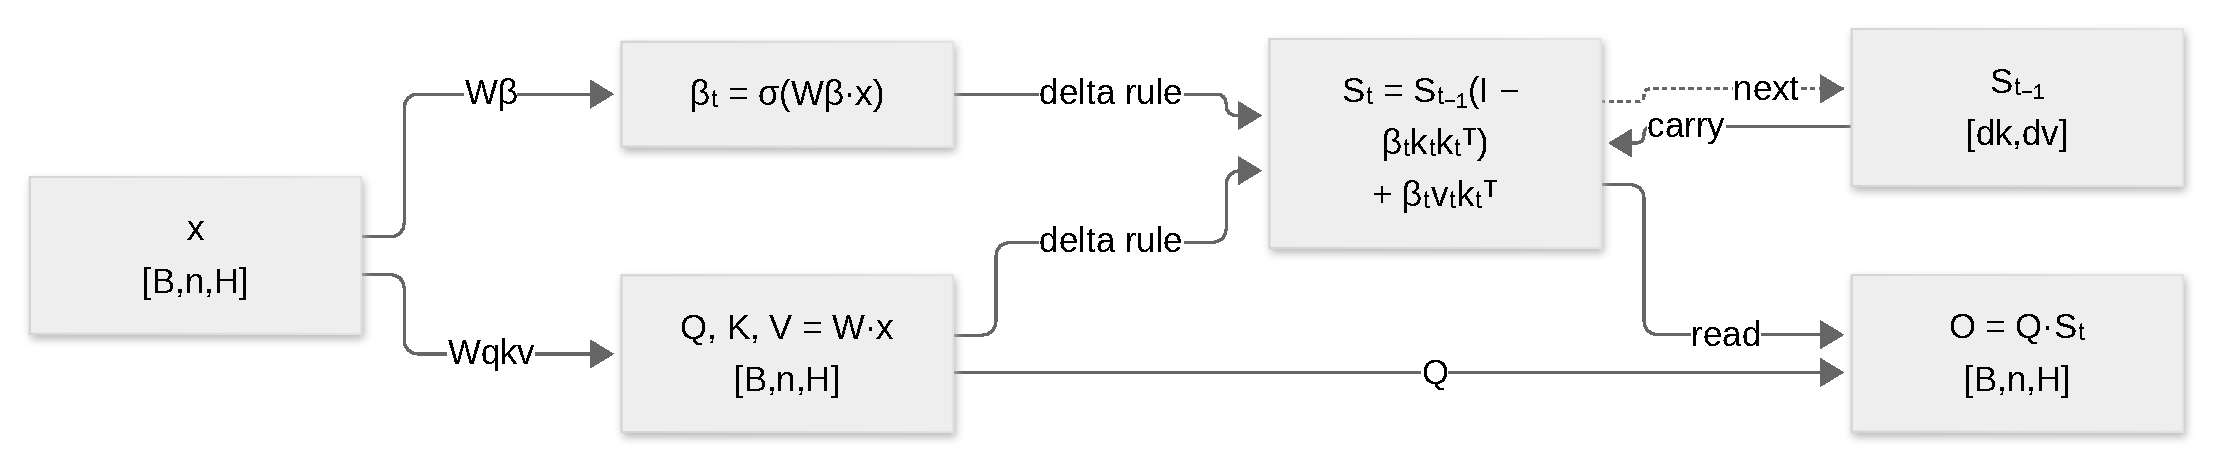
\includegraphics{../paper/figures/mixers/deltanet.pdf}}
\caption{Flujo de datos de DeltaNet: la compuerta beta aplica una regla delta correctora de errores al estado recurrente.}
\label{fig:mixer-deltanet}
\end{figure}

\subsubsection{Fundamento Matemático}

DeltaNet \citep{yang_deltanet_2024} aplica una \textbf{regla de aprendizaje delta} clásica a las actualizaciones de estado de la atención lineal. En lugar de acumulación aditiva, DeltaNet calcula la diferencia entre el valor predicho (recuperado de la memoria) y el valor objetivo, luego realiza una actualización de corrección de errores:
\[
\mathbf{S}_t = \mathbf{S}_{t-1}(\mathbf{I} - \beta_t \mathbf{k}_t \mathbf{k}_t^\top) + \beta_t \mathbf{v}_t \mathbf{k}_t^\top
\]
donde $\beta_t \in (0,1)$ es un escalar de \textbf{intensidad de escritura} dependiente de los datos. Esta actualización puede descomponerse como una operación de borrado-escritura:
\[
\mathbf{v}_t^\text{anterior} = \mathbf{S}_{t-1} \mathbf{k}_t \quad \text{(predicción actual)}, \quad
\mathbf{v}_t^\text{actualizado} = \beta_t \mathbf{v}_t + (1-\beta_t)\mathbf{v}_t^\text{anterior} \quad \text{(mezcla anterior/nuevo)}
\]
de modo que:
\[
\mathbf{S}_t = \mathbf{S}_{t-1} - \mathbf{v}_t^\text{anterior}\mathbf{k}_t^\top + \mathbf{v}_t^\text{actualizado}\mathbf{k}_t^\top
\]

La idea clave es que esta regla de actualización minimiza una pérdida de ECM en línea en cada paso temporal:
\[
\mathcal{L}_t(\mathbf{S}) = \tfrac{1}{2}\|\mathbf{S}\mathbf{k}_t - \mathbf{v}_t\|^2 \Rightarrow \nabla_{\mathbf{S}} \mathcal{L}_t = (\mathbf{S}\mathbf{k}_t - \mathbf{v}_t)\mathbf{k}_t^\top
\]

Un paso de SGD con tasa de aprendizaje $\beta_t$ produce la actualización de la regla delta. Esta conexión con el entrenamiento en tiempo de prueba (TTT) proporciona fundamentación teórica: DeltaNet optimiza directamente la predicción de valores en tiempo de inferencia.

\subsubsection{Entrenamiento Paralelo Eficiente}

La matriz de transición de DeltaNet $\mathbf{I} - \beta_t \mathbf{k}_t \mathbf{k}_t^\top$ es una matriz de Householder generalizada (actualización de rango 1 a la identidad). Para el entrenamiento por fragmentos, DeltaNet usa la \textbf{representación WY}, que representa el producto de $m$ de estas actualizaciones de rango 1 de forma compacta:
\[
\prod_{i=1}^{m} (\mathbf{I} - \beta_i \mathbf{k}_i \mathbf{k}_i^\top) = \mathbf{I} - \mathbf{W}\mathbf{Y}^\top
\]
donde $\mathbf{W}, \mathbf{Y} \in \mathbb{R}^{d \times m}$ se construyen recursivamente. Esta factorización permite paralelismo rico en matmul sin materializar el producto completo, manteniendo el entrenamiento por fragmentos eficiente.

\begin{algorithm}[H]
\caption{Actualización de Estado de DeltaNet con Representación WY}
\begin{algorithmic}[1]
\Require Fragmento de entrada $\mathbf{X}_{[t]}$; estado anterior $\mathbf{S}_{t-1}$
\Require Consultas normalizadas L2 $\hat{\mathbf{Q}}_t$, claves $\hat{\mathbf{K}}_t$, valores $\mathbf{V}_t$
\Ensure Salida $\mathbf{O}_{[t]}$ y estado actualizado $\mathbf{S}_t$
\State \textbf{Fase por fragmentos:}
\For{posición $i = 1$ to tamaño\_fragmento}
    \State Normalizar: $\hat{\mathbf{k}}_i \gets \hat{\mathbf{K}}_t[i] / \|\hat{\mathbf{K}}_t[i]\|$, $\hat{\mathbf{q}}_i \gets \hat{\mathbf{Q}}_t[i] / \|\hat{\mathbf{Q}}_t[i]\|$
    \State Calcular intensidad de escritura: $\beta_i \gets \text{sigmoid}(W_\beta \mathbf{x}_i)$
    \State Predicción: $\hat{\mathbf{v}}^\text{pred} \gets \mathbf{S}_{i-1}^\text{en-fragmento} \hat{\mathbf{k}}_i$
    \State Mezcla consciente del error: $\mathbf{v}_i^\text{actualización} \gets \beta_i(\mathbf{v}_i - \hat{\mathbf{v}}^\text{pred})$
    \State Borrar-escribir: $\mathbf{S}_i^\text{en-fragmento} \gets \mathbf{S}_{i-1}^\text{en-fragmento} - \hat{\mathbf{v}}^\text{pred}\hat{\mathbf{k}}_i^\top + (\beta_i \mathbf{v}_i + (1-\beta_i)\hat{\mathbf{v}}^\text{pred})\hat{\mathbf{k}}_i^\top$
    \State Salida: $\mathbf{o}_i \gets \mathbf{S}_i^\text{en-fragmento} \hat{\mathbf{q}}_i$
\EndFor
\State \textbf{Fase entre fragmentos:} Usar representación WY de los productos de transición
\Return $\mathbf{O}_{[t]}$, $\mathbf{S}_{t}$
\end{algorithmic}
\end{algorithm}

\subsubsection{Fortalezas y Limitaciones}

\begin{table}[H]
\centering
\small
\begin{tabularx}{0.95\linewidth}{Xp{4cm}p{4cm}}
\toprule
\textbf{Aspecto} & \textbf{Fortalezas} & \textbf{Limitaciones} \\
\midrule
Recuperación asociativa & Recuperación perfecta en el benchmark MQAR (Recuperación Asociativa Multi-Consulta); la semántica de corrección de errores se ajusta naturalmente a patrones de recuperación. & Sin olvido global, la memoria aún se satura en longitudes de secuencia extremas; requiere mecanismos de reinicio periódico para contexto ilimitado. \\
Teoría & Fundamentada en optimización de ECM en línea; conexión clara con el paradigma de entrenamiento en tiempo de prueba. & Requiere claves normalizadas L2 para estabilidad numérica; la normalización de doble ancho añade sobrecarga. \\
Rendimiento & La representación WY permite entrenamiento eficiente por fragmentos. & Ligeramente más lento que Mamba2 por token debido a matrices de transición más ricas (rango 1 en lugar de diagonales). \\
\bottomrule
\end{tabularx}
\end{table}

\subsection{3. Gated DeltaNet: Síntesis de Compuerta y Corrección de Errores}

\begin{figure}[H]
\centering
\fitfigure{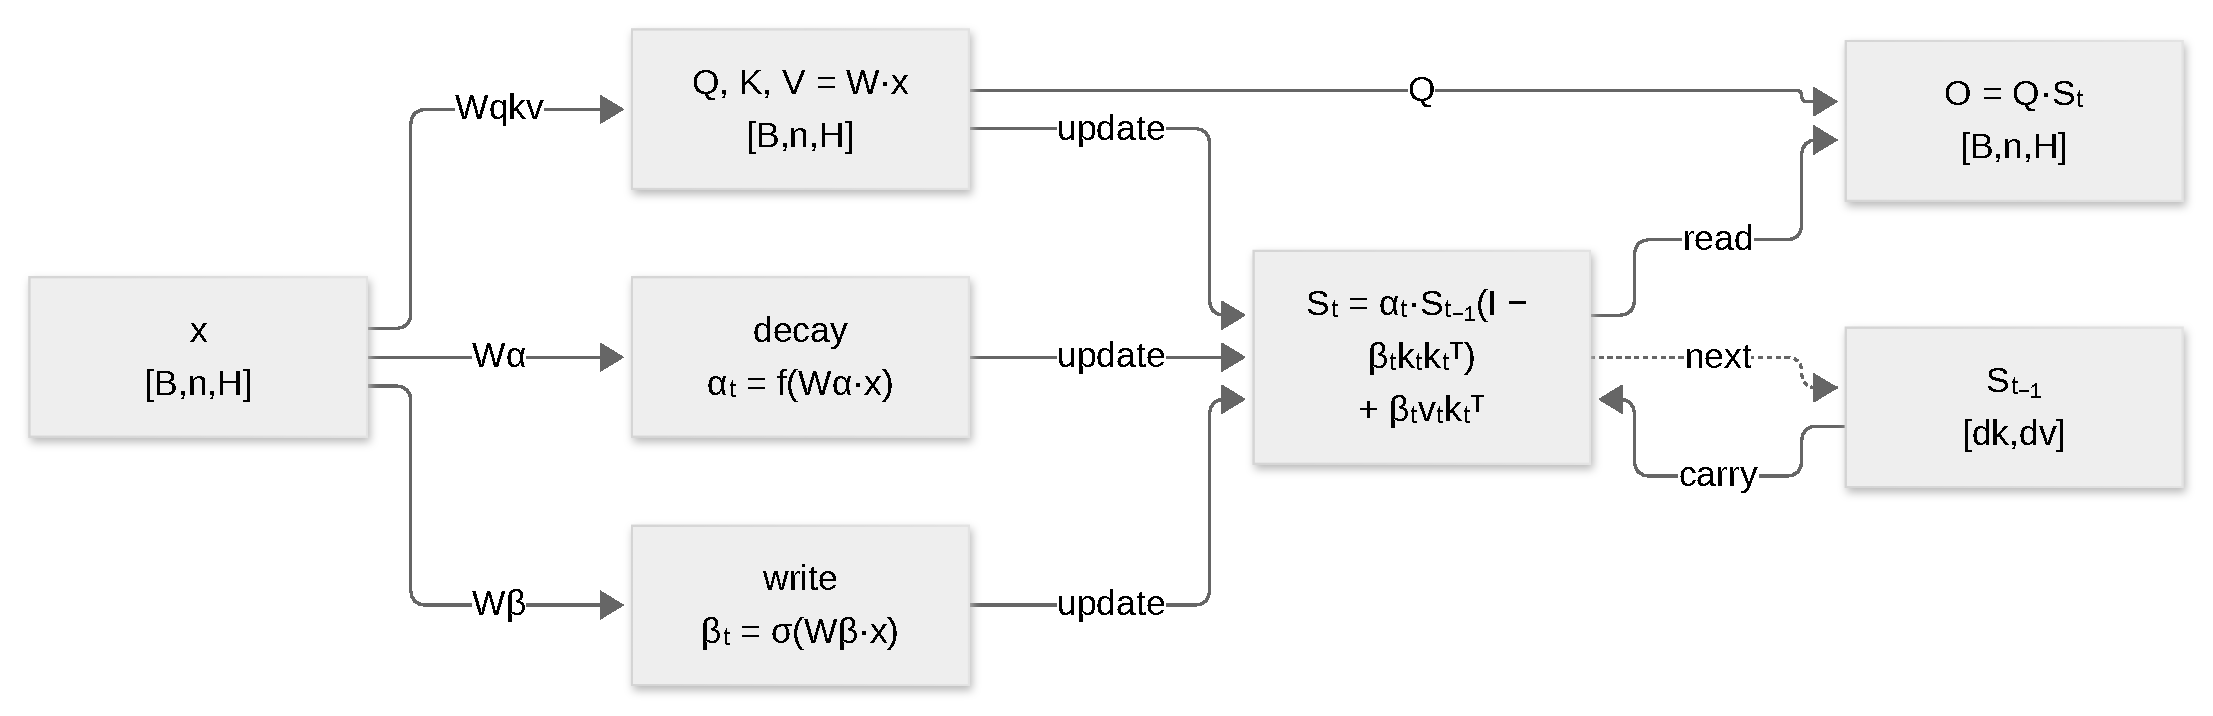
\includegraphics{../paper/figures/mixers/gated-deltanet.pdf}}
\caption{Flujo de datos de Gated DeltaNet: las compuertas de decaimiento y escritura modulan la actualización del estado por regla delta.}
\label{fig:mixer-gated-deltanet}
\end{figure}

\subsubsection{Fundamento Matemático}

Gated DeltaNet \citep{yang_gated_deltanet_2024} sintetiza las fortalezas de GLA y DeltaNet combinando una \textbf{compuerta de decaimiento} $\alpha_t$ (de GLA) con la \textbf{compuerta de intensidad de escritura} $\beta_t$ (de DeltaNet):
\[
\mathbf{S}_t = \mathbf{S}_{t-1}\left(\alpha_t (\mathbf{I} - \beta_t \mathbf{k}_t \mathbf{k}_t^\top)\right) + \beta_t \mathbf{v}_t \mathbf{k}_t^\top
\]
Reescribiendo para mayor claridad:
\[
\mathbf{S}_t = \alpha_t \mathbf{S}_{t-1}(\mathbf{I} - \beta_t \mathbf{k}_t \mathbf{k}_t^\top) + \beta_t \mathbf{v}_t \mathbf{k}_t^\top
\]
Las dos compuertas son complementarias:
\begin{itemize}[leftmargin=*]
    \item $\alpha_t \to 0$ borra rápidamente el estado histórico: $\mathbf{S}_t \approx \beta_t \mathbf{v}_t \mathbf{k}_t^\top$ (reinicio de contexto).
    \item $\alpha_t \to 1$ recupera el comportamiento puro de regla delta: $\mathbf{S}_t \approx \mathbf{S}_{t-1}(\mathbf{I} - \beta_t \mathbf{k}_t \mathbf{k}_t^\top) + \beta_t \mathbf{v}_t \mathbf{k}_t^\top$ (actualizaciones dirigidas).
    \item $\beta_t \to 0$ omite la escritura pero decae: $\mathbf{S}_t \approx \alpha_t \mathbf{S}_{t-1}$ (olvido puro).
    \item $\beta_t \to 1$ reemplaza la memoria agresivamente: $\mathbf{S}_t \approx \alpha_t \mathbf{S}_{t-1} + \mathbf{v}_t \mathbf{k}_t^\top$ (reemplazo).
\end{itemize}

Desde una perspectiva de aprendizaje en línea, Gated DeltaNet corresponde a:
\[
\min_{\mathbf{S}_t} \|\mathbf{S}_t - \alpha_t \mathbf{S}_{t-1}\|_F^2 - 2\langle \mathbf{S}_t \mathbf{k}_t, \beta_t(\mathbf{v}_t - \alpha_t \mathbf{S}_{t-1} \mathbf{k}_t)\rangle
\]
que introduce un decaimiento de pesos adaptativo $\alpha_t$ en una actualización tipo SGD---análogo al decaimiento de pesos desacoplado en la optimización de aprendizaje profundo.

\begin{algorithm}[H]
\caption{Paso Adelante Paralelo por Fragmentos de Gated DeltaNet}
\begin{algorithmic}[1]
\Require Fragmento de entrada $\mathbf{X}_{[i]}$; estado anterior $\mathbf{S}_{i-1}$; tamaño de fragmento $C$
\Require Proyecciones: $W_q, W_k, W_v, W_\alpha, W_\beta$
\Ensure Salida $\mathbf{O}_{[i]}$ y estado $\mathbf{S}_i$
\State \textbf{Cálculo en-fragmento:}
\For{$j = 1$ to $C$}
    \State $\mathbf{q}_j \gets W_q \mathbf{x}_j$, $\mathbf{k}_j \gets W_k \mathbf{x}_j$, $\mathbf{v}_j \gets W_v \mathbf{x}_j$
    \State $\alpha_j \gets \text{sigmoid}(W_\alpha \mathbf{x}_j)$, $\beta_j \gets \text{sigmoid}(W_\beta \mathbf{x}_j)$
    \State Aplicar compuerta combinada: $\mathbf{S}_j \gets \alpha_j \mathbf{S}_{j-1}(\mathbf{I} - \beta_j \mathbf{k}_j \mathbf{k}_j^\top) + \beta_j \mathbf{v}_j \mathbf{k}_j^\top$
    \State $\mathbf{o}_j \gets \mathbf{S}_j \mathbf{q}_j$
\EndFor
\State \textbf{Recurrencia entre fragmentos:}
\State $\mathbf{S}_i \gets \mathbf{S}_C$ del en-fragmento; propagar entre fragmentos mediante máscaras $\prod \alpha$ acumulativas
\State \textbf{Compuerta de salida:} $\mathbf{O}_{[i]} \gets \text{GroupNorm}(\mathbf{O}^\text{crudo}) \otimes \text{SiLU}(W_g \mathbf{X}_{[i]})$
\Return $\mathbf{O}_{[i]}$, $\mathbf{S}_i$
\end{algorithmic}
\end{algorithm}

\subsubsection{Rendimiento Empírico y Compensaciones}

Gated DeltaNet se ha integrado en los modelos de producción Qwen3-Next y Qwen3.5 de Alibaba. Empíricamente:
\[
\begin{array}{l|cccc}
\textbf{Tarea} & \textbf{Gated DeltaNet} & \textbf{Mamba2} & \textbf{DeltaNet} & \textbf{GLA} \\
\hline
\text{Modelado de Lenguaje} & \mathbf{1.0\times} & 1.08\times & 1.05\times & 1.12\times \\
\text{Recuperación Asociativa} & \mathbf{1.0\times} & --(sin perfecto) & \mathbf{1.0\times} & 0.75 \\
\text{Extrapolación de Longitud} & \mathbf{1.0\times} & 0.98\times & 0.96\times & 0.94\times \\
\text{Rendimiento (tokens/seg)} & 0.85\times & \mathbf{1.0\times} & 0.82\times & 0.88\times
\end{array}
\]
Gated DeltaNet logra el mejor equilibrio entre diversas tareas a costa de un rendimiento ligeramente reducido debido a matrices de transición más ricas.

\subsection{4. HGRN2: Compuerta Jerárquica con Expansión de Producto Externo}

\begin{figure}[H]
\centering
\fitfigure{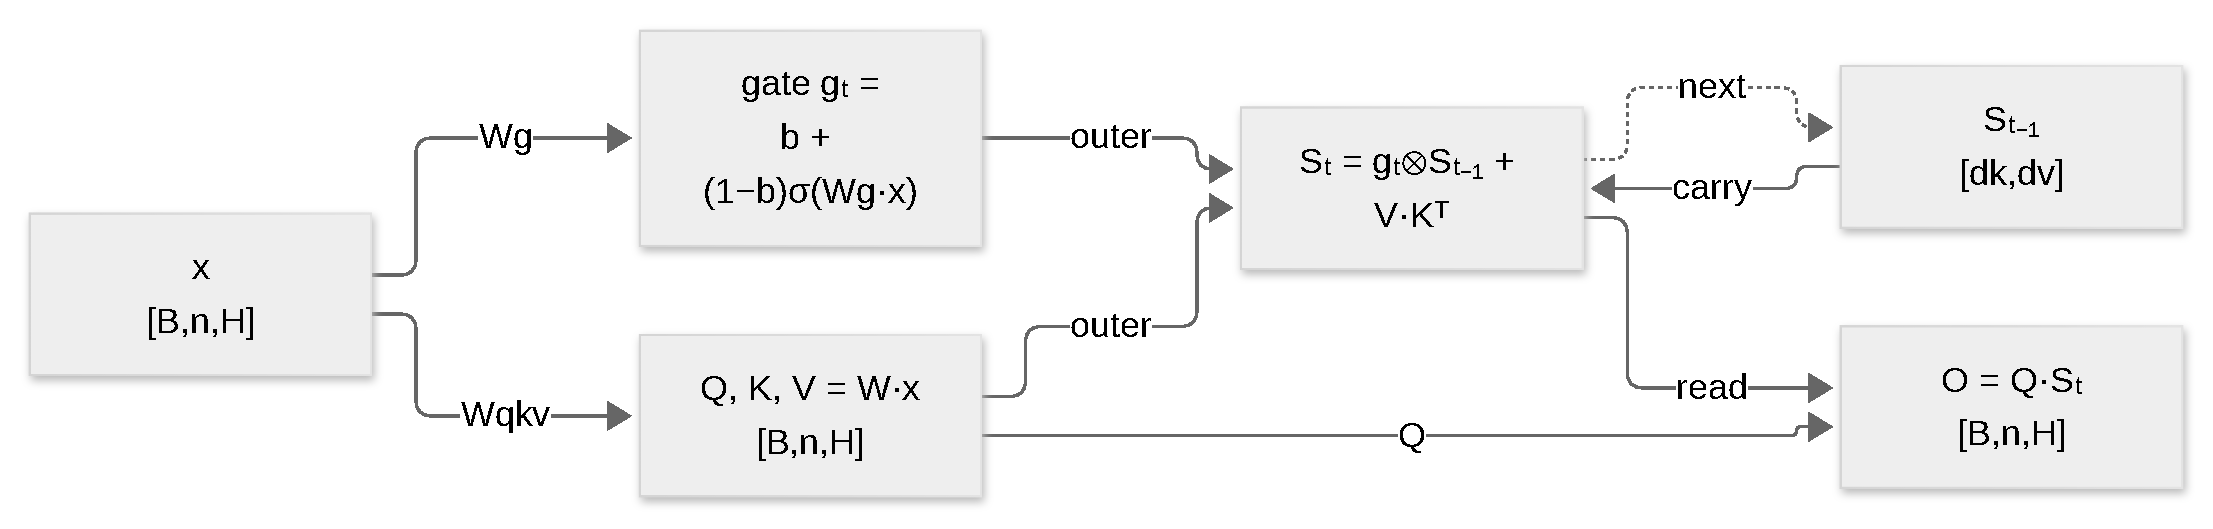
\includegraphics{../paper/figures/mixers/hgrn2.pdf}}
\caption{Flujo de datos de HGRN2: una compuerta jerárquica mezcla el estado transportado con el producto externo clave/valor.}
\label{fig:mixer-hgrn2}
\end{figure}

\subsubsection{Fundamento Matemático}

HGRN2 \citep{qin_hgrn2_2024} usa una expansión de estado basada en producto externo con \textbf{compuertas de olvido acotadas inferiormente de forma jerárquica}. La actualización de estado es:
\[
\mathbf{S}_t = \text{diag}(\mathbf{g}_t) \cdot \mathbf{S}_{t-1} + \mathbf{v}_t \mathbf{k}_t^\top, \quad \mathbf{o}_t = \mathbf{S}_t \mathbf{q}_t
\]
donde $\mathbf{g}_t \in [b_\ell, 1]^d$ es una compuerta de olvido con cota inferior para la capa $\ell$. Las cotas satisfacen:
\[
0 \le b_{\ell_{\text{poco profunda}}} < b_{\ell_{\text{media}}} < b_{\ell_{\text{profunda}}} \le 1
\]
es decir, las cotas aumentan (se vuelven menos restrictivas) en las capas más profundas. La compuerta en sí se calcula como:
\[
\mathbf{g}_t = b_\ell + (1 - b_\ell) \cdot \sigma(W_g \mathbf{x}_t)
\]
donde $\sigma$ es sigmoide. Cuando $W_g$ produce logits débilmente negativos, $\mathbf{g}_t \approx b_\ell$ (retención forzada en capas superficiales). Cuando las salidas son fuertemente positivas, $\mathbf{g}_t \approx 1$ (refresco de memoria en cualquier capa).

La estructura jerárquica anima a diferentes capas a especializarse en diferentes escalas temporales: las capas superficiales modelan dependencias locales (alta retención debido a la cota $b_\ell$), mientras que las capas profundas capturan estructura de largo alcance (compuerta flexible con cota superior alta).

\begin{algorithm}[H]
\caption{Paso Adelante de HGRN2 con Cotas Jerárquicas}
\begin{algorithmic}[1]
\Require Entrada $\mathbf{x}_t$; estado anterior $\mathbf{S}_{t-1}$; índice de capa $\ell \in [0, L-1]$
\Require Cotas no decrecientes: $0 \le b_0 < b_1 < \cdots < b_{L-1} \le 1$
\Ensure Salida $\mathbf{o}_t$ y estado $\mathbf{S}_t$
\State Cota de retención específica de capa: $b \gets b_\ell$
\State Proyectar: $\mathbf{q}_t \gets W_q \mathbf{x}_t$, $\mathbf{k}_t \gets W_k \mathbf{x}_t$, $\mathbf{v}_t \gets W_v \mathbf{x}_t$
\State Calcular compuerta de olvido con cota: $\mathbf{g}_t \gets b + (1-b) \cdot \sigma(W_g \mathbf{x}_t)$ \Comment{Confinado a $[b, 1]$}
\State Multiplicación diagonal (vectorizada): $\mathbf{S}_t \gets \mathbf{S}_{t-1} \circ \text{diag}(\mathbf{g}_t) + \mathbf{v}_t \mathbf{k}_t^\top$
\State Recuperar: $\mathbf{o}_t \gets \mathbf{S}_t \mathbf{q}_t$
\State Normalización opcional: $\mathbf{o}_t \gets \text{RMSNorm}(\mathbf{o}_t)$
\Return $\mathbf{o}_t$, $\mathbf{S}_t$
\end{algorithmic}
\end{algorithm}

\subsubsection{Escalado y Resultados Empíricos}

A escala de 3B en 100B tokens, HGRN2 supera ligeramente a Mamba2 y a los Transformers con arquitectura LLaMA en modelado de lenguaje. La compuerta jerárquica proporciona modelado temporal multi-escala sin variantes arquitectónicas explícitas por capa. Sin embargo, la compuerta diagonal con valor vectorial (en oposición a la selección elemento a elemento) proporciona menos flexibilidad por elemento que las variantes de regla delta.

\subsection{5. Forgetting Transformer (FoX): Compuerta en el Espacio de Logits Softmax}

\begin{figure}[H]
\centering
\fitfigure{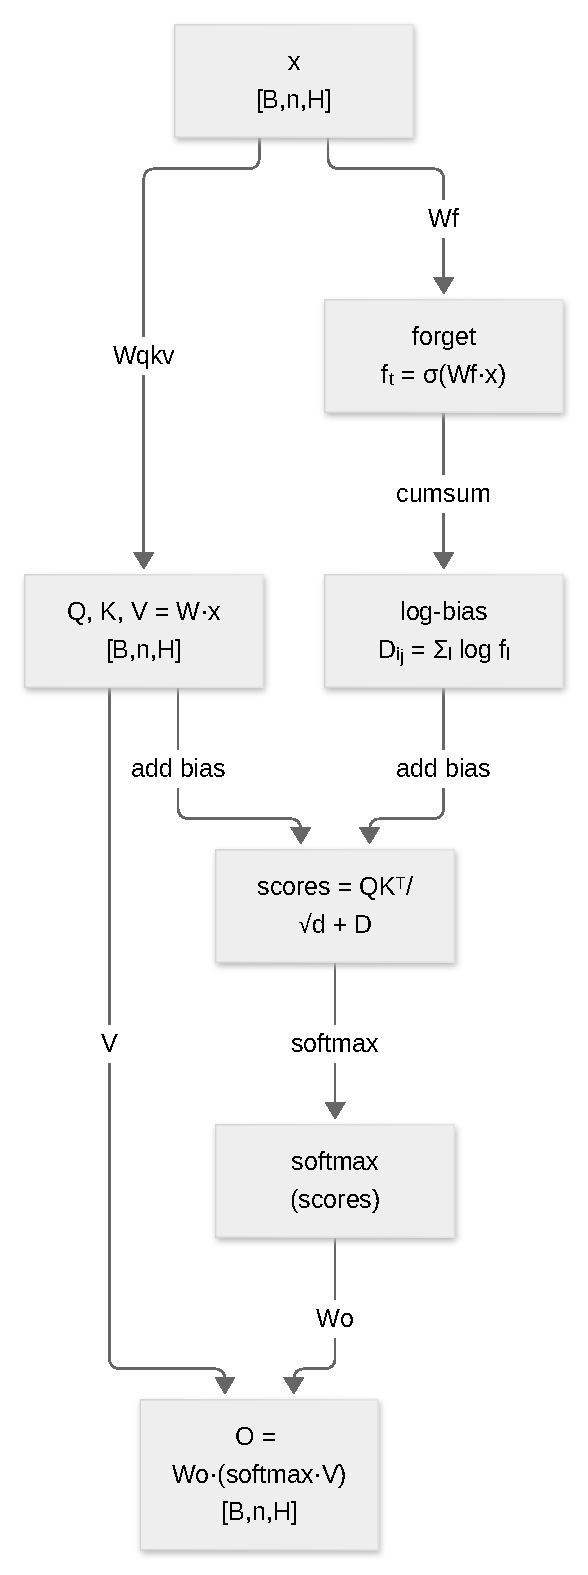
\includegraphics{../paper/figures/mixers/fox.pdf}}
\caption{Flujo de datos de FoX: una compuerta de olvido aprendida se convierte en un sesgo aditivo en el espacio de logits.}
\label{fig:mixer-fox}
\end{figure}

\subsubsection{Fundamento Matemático}

Forgetting Transformer (FoX), propuesto por Lin et al.~\citep{lin_forgetting_transformer_2025}, incrusta una compuerta de olvido directamente en los logits de atención softmax. En lugar de reemplazar softmax con recurrencia lineal, FoX preserva la expresividad completa de softmax mientras añade control de actualidad mediante un sesgo de logit dependiente de los datos.

Para cada posición de token $t$ y todas las claves $j \le t$, calcular un escalar de compuerta de olvido:
\[
f_t = \sigma(w_f^\top \mathbf{x}_t + b_f)
\]
El sesgo de logit en la posición $(i,j)$ es el producto acumulativo log-olvido:
\[
d_{ij} = \sum_{l=j+1}^{i} \log f_l = \log \prod_{l=j+1}^{i} f_l
\]
La salida de atención completa se convierte en:
\[
\mathbf{O} = \text{softmax}\left(\frac{\mathbf{Q}\mathbf{K}^\top}{\sqrt{d_k}} + \mathbf{D}\right) \mathbf{V}
\]
donde $\mathbf{D}_{ij} = d_{ij}$. Equivalentemente:
\[
\text{Atencion}(i,j) = \frac{\exp(\mathbf{q}_i^\top \mathbf{k}_j / \sqrt{d_k} + d_{ij})}{\sum_{j'=1}^{i} \exp(\mathbf{q}_i^\top \mathbf{k}_{j'} / \sqrt{d_k} + d_{ij'})}
\]

Esta ponderación reduce el peso de los tokens más antiguos multiplicativamente: un token de hace 10 pasos se escala por $\prod_{l=j+1}^{i} f_l$, que es típicamente mucho menor que 1 si $f_t < 1$ en promedio.

El mecanismo es matemáticamente equivalente a una \textbf{variante aprendible dependiente de los datos de ALiBi (Atención con Sesgos Lineales)}, donde trabajos anteriores usaban $d_{ij} = -\infty \cdot |i-j|$ fijo o $d_{ij} = -(i-j)$.

\begin{algorithm}[H]
\caption{FoX: Atención con Olvido y Sesgo de Actualidad}
\begin{algorithmic}[1]
\Require Consultas $\mathbf{Q}$, claves $\mathbf{K}$, valores $\mathbf{V}$; entrada $\mathbf{X}$
\Require Parámetros de compuerta de olvido: $w_f \in \mathbb{R}^d$, $b_f \in \mathbb{R}$
\Ensure Salida de atención $\mathbf{O}$
\State \textbf{Calcular compuertas de olvido:}
\For{$t = 1$ to $T$}
    \State $f_t \gets \sigma(w_f^\top \mathbf{x}_t + b_f)$ \Comment{Probabilidad de olvido por token}
\EndFor
\State \textbf{Calcular sesgos acumulativos de log-olvido:}
\For{$i = 1$ to $T$}
    \For{$j = 1$ to $i$}
        \State $d_{ij} \gets \sum_{l=j+1}^{i} \log f_l$ \Comment{Producto acumulativo en espacio logarítmico}
    \EndFor
\EndFor
\State \textbf{SDPA estándar con sesgo:}
\State Calcular puntajes: $\mathbf{S} \gets \mathbf{Q}\mathbf{K}^\top / \sqrt{d_k}$
\State Agregar sesgo: $\mathbf{S} \gets \mathbf{S} + \mathbf{D}$
\State Aplicar softmax: $\mathbf{A} \gets \text{softmax}(\mathbf{S}, \text{dim}=-1)$
\State Ponderar valores: $\mathbf{O} \gets \mathbf{A} \mathbf{V}$
\Return $\mathbf{O}$
\end{algorithmic}
\end{algorithm}

\subsubsection{Integración con FlashAttention}

La ventaja clave de FoX es la compatibilidad con FlashAttention y las implementaciones optimizadas existentes. Los sesgos de olvido se añaden en el cálculo de logits softmax, que ya es una operación central en el algoritmo por bloques de FlashAttention. La sobrecarga es:
\[
\text{Sobrecarga} \approx 0.5--2\% \text{ del tiempo de pared}
\]
ya que la adición de sesgo se amortiza entre las operaciones matmul.

\subsubsection{Fortalezas y Limitaciones}

FoX logra resultados de última generación en extrapolación de longitud, recuperación casi perfecta de aguja en el pajar y comprensión superior de contexto largo en comparación con los Transformers. Sin embargo, sigue siendo $\mathcal{O}(L^2 d)$ en entrenamiento y $\mathcal{O}(L d)$ por paso en inferencia con caché KV, limitando las longitudes de secuencia extremas.

\subsection{6. Atención con Compuerta (Post-SDPA Sigmoide)}

\begin{figure}[H]
\centering
\fitfigure{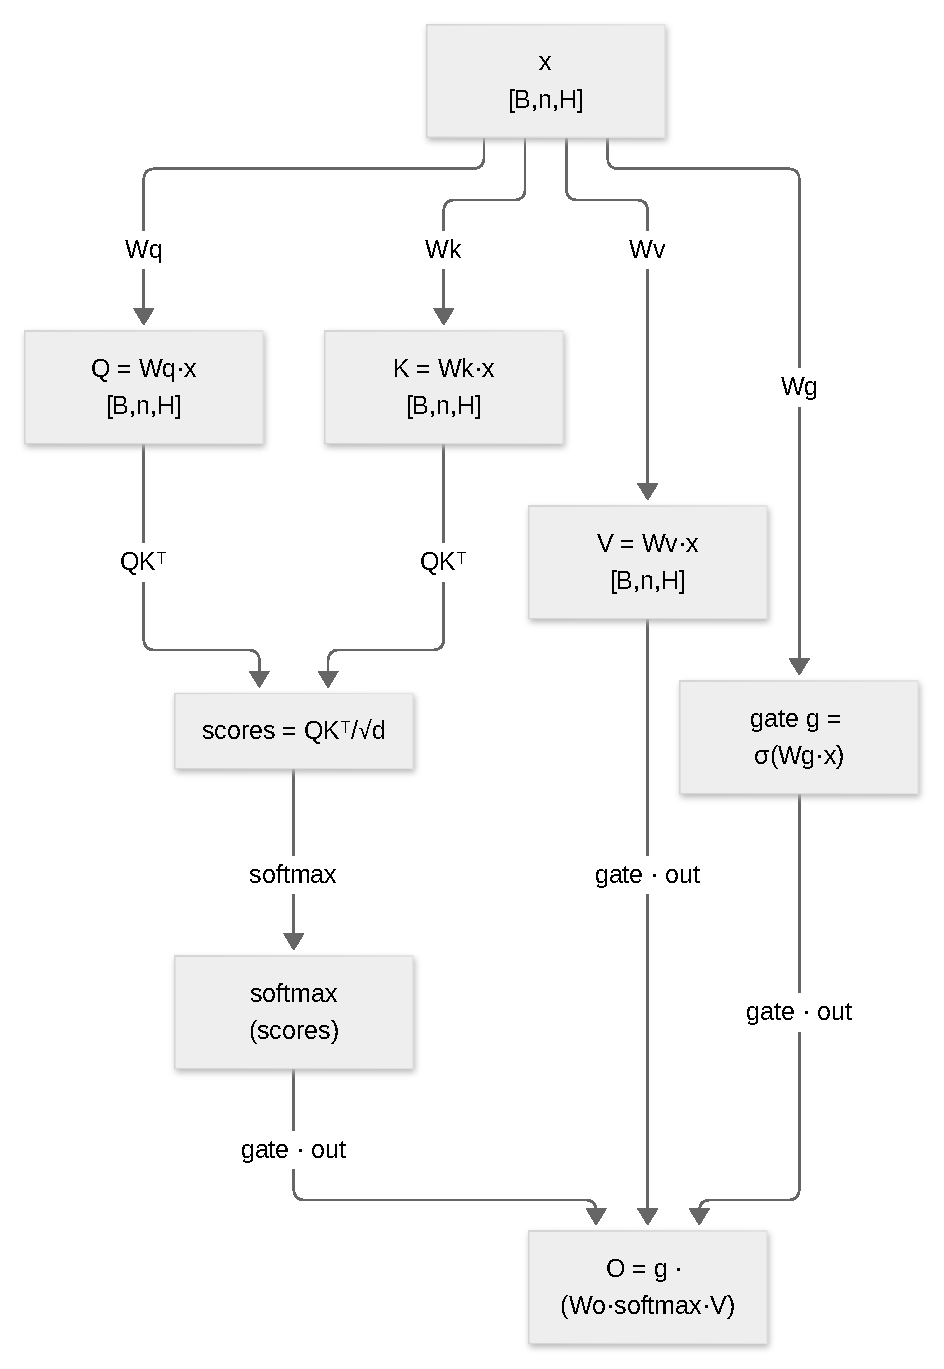
\includegraphics{../paper/figures/mixers/gated-softmax.pdf}}
\caption{Flujo de datos de la atención con compuerta posterior a SDPA: una compuerta sigmoide escala la salida del softmax antes de la proyección.}
\label{fig:mixer-gated-softmax}
\end{figure}

\subsubsection{Fundamento Matemático}

El Mejor Artículo de NeurIPS 2025 del equipo de Qwen propone aplicar una compuerta sigmoide \textbf{después} de la atención de producto punto escalado (SDPA):
\[
\mathbf{Y} = \text{SDPA}(\mathbf{Q}, \mathbf{K}, \mathbf{V}) = \text{softmax}\left(\frac{\mathbf{Q}\mathbf{K}^\top}{\sqrt{d_k}}\right) \mathbf{V}
\]
\[
\mathbf{Y}' = \mathbf{Y} \odot \sigma\left(\mathbf{X} \mathbf{W}_\theta\right)
\]
donde el puntaje de compuerta $\sigma(\mathbf{X} \mathbf{W}_\theta)$ puede tener forma $\mathbb{R}^{n \times q \times d_k}$ (compuerta elemento a elemento por cabeza de consulta) o $\mathbb{R}^{n \times q}$ (compuerta fija por cabeza). En más de 30 variantes y modelos MoE de 15B + densos de 1.7B entrenados en 3.5T tokens, el equipo encontró:

\begin{itemize}[leftmargin=*]
    \item La compuerta por cabeza añade solo $\sim 1.6M$ parámetros a un modelo de 15B (sobrecarga insignificante).
    \item Las compuertas efectivas son \textbf{dispersas}: activación media $\approx 0.116$ (es decir, el 88\% son cero o casi cero).
    \item Las compuertas actúan como filtros dependientes de la consulta, suprimiendo canales de bajo valor mientras preservan señales de alto valor.
    \item Las compuertas eliminan demostrablemente el fenómeno de \textbf{sumidero de atención}, donde el patrón de atención se vuelve dominado por un único token temprano.
\end{itemize}

\begin{algorithm}[H]
\caption{Atención Softmax con Compuerta (Post-SDPA)}
\begin{algorithmic}[1]
\Require Consultas $\mathbf{Q}$, Claves $\mathbf{K}$, Valores $\mathbf{V}$; entrada $\mathbf{X}$
\Require Matriz de proyección de compuerta $W_g \in \mathbb{R}^{d \to d_{\text{compuerta}}}$ donde $d_{\text{compuerta}} \in \{1, d_k\}$
\Ensure Salida con compuerta $\mathbf{Y}'$
\State \textbf{SDPA estándar:}
\State Calcular atención: $\mathbf{A} \gets \text{softmax}(\mathbf{Q}\mathbf{K}^\top / \sqrt{d_k})$ 
\State Ponderar valores: $\mathbf{Y} \gets \mathbf{A} \mathbf{V}$
\State \textbf{Calcular compuertas:}
\State Proyectar entrada: $\mathbf{G} \gets \mathbf{X} W_g$  \Comment{forma: $[n, q, d_{\text{compuerta}}]$}
\State Aplicar sigmoide: $\mathbf{G} \gets \sigma(\mathbf{G})$ \Comment{Compuerta elemento a elemento}
\State \textbf{Aplicar compuerta:}
\If{$d_{\text{compuerta}} = 1$}
    \State Transmitir y escalar: $\mathbf{Y}' \gets \mathbf{Y} \cdot \mathbf{G}$ \Comment{Escalado por cabeza}
\Else
    \Comment{$d_{\text{compuerta}} = d_k$}
    \State Modulación elemento a elemento: $\mathbf{Y}' \gets \mathbf{Y} \odot \mathbf{G}$ \Comment{Compuerta por dimensión}
\EndIf
\Return $\mathbf{Y}'$
\end{algorithmic}
\end{algorithm}

\subsubsection{Hallazgos Clave}

\begin{itemize}[leftmargin=*]
    \item \textbf{Supresión del sumidero de atención}: La compuerta rompe el ciclo de retroalimentación donde softmax se concentra en el primer token, permitiendo una atención más equilibrada.
    \item \textbf{Estabilidad de entrenamiento}: Los modelos con compuerta toleran tasas de aprendizaje más grandes ($+30\%$ mayor $\eta_{max}$ estable).
    \item \textbf{Sobrecarga mínima}: El impacto en latencia es solo del $1.6\%$ en GPUs H100; el rendimiento cae como máximo $2-3\%$.
    \item \textbf{Mejora en la ley de escalado}: Mejora la pérdida en todas las escalas de modelo, desde 800M hasta 110B parámetros de forma consistente.
\end{itemize}

\normalsize

\subsection{7. Gated DeltaNet-2: Borrado y Escritura Canalizados Decouplados}

\begin{figure}[H]
\centering
\fitfigure{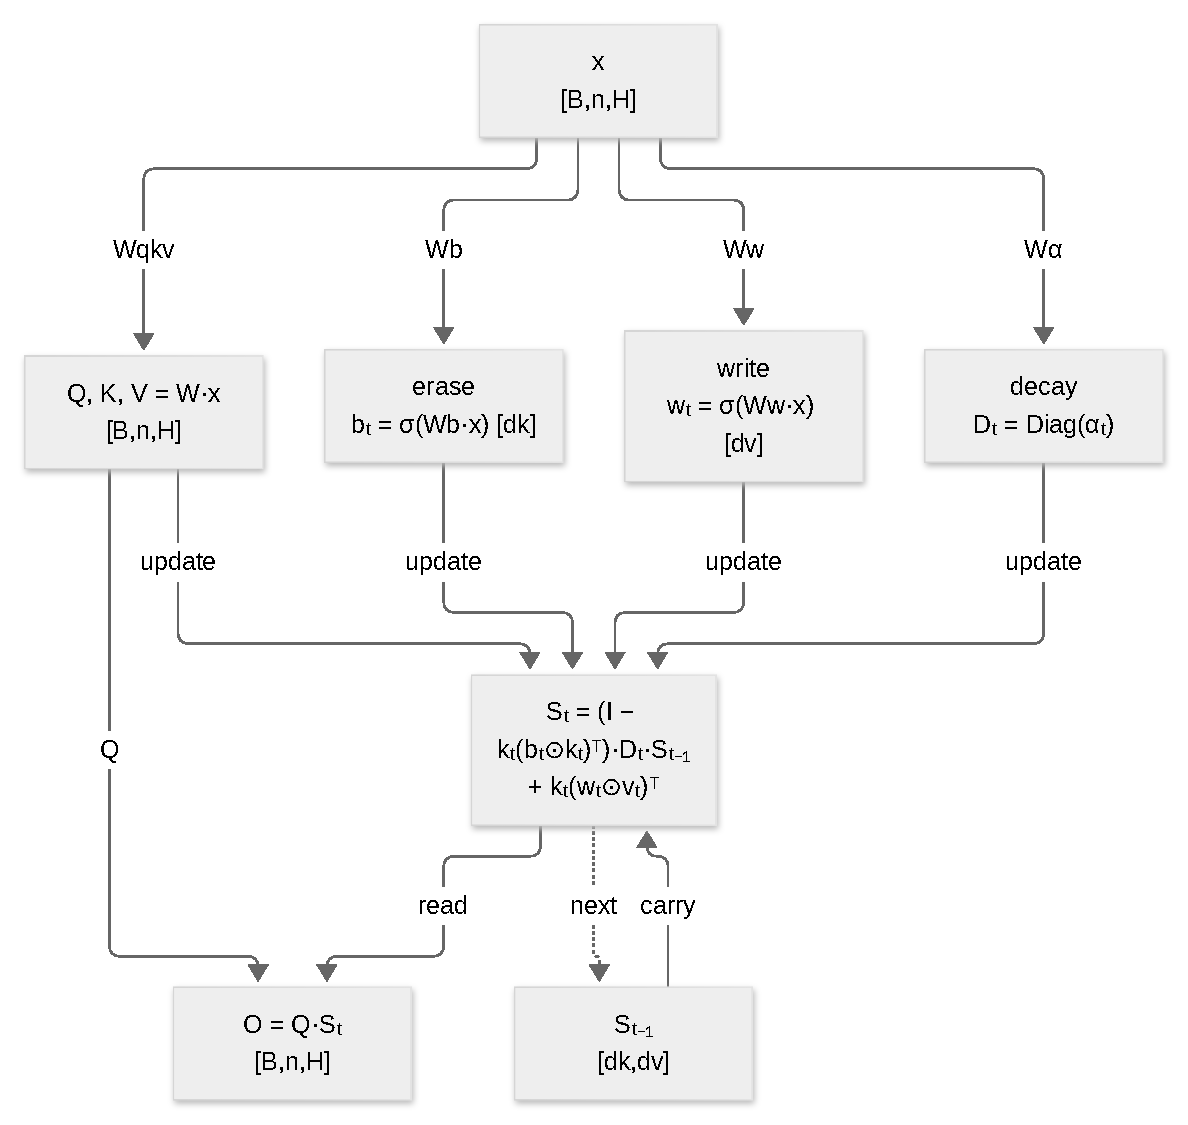
\includegraphics{../paper/figures/mixers/gated-deltanet2.pdf}}
\caption{Flujo de datos de Gated DeltaNet-2: compuertas desacopladas de borrado y escritura por canal actúan dentro de la regla delta.}
\label{fig:mixer-gated-deltanet2}
\end{figure}

\subsubsection{Fundamento Matemático}

Gated DeltaNet-2 \citep{hatamizadeh_gated_deltanet2_2026} aborda una limitación compartida de Gated DeltaNet y Kimi Delta Attention (KDA): ambos usan una única \emph{compuerta delta escalar} $\beta_t$ para controlar simultáneamente (i) cuánto contenido antiguo se borra en la dirección de lectura del eje de claves y (ii) cuánto valor nuevo se escribe en el eje de valores. Gated DeltaNet-2 \textbf{desacopla} estos dos roles en una compuerta de borrado canalizada $\mathbf{b}_t$ (eje de claves) y una compuerta de escritura canalizada $\mathbf{w}_t$ (eje de valores), heredando además el decaimiento canalizado $\boldsymbol{\alpha}_t$ de KDA. Con estado $\mathbf{S}_t \in \mathbb{R}^{d_k \times d_v}$, decaimiento $\mathbf{D}_t = \mathrm{Diag}(\boldsymbol{\alpha}_t)$, dirección de borrado $\mathbf{e}_t = \mathbf{b}_t \odot \mathbf{k}_t$ y objetivo de escritura $\mathbf{z}_t = \mathbf{w}_t \odot \mathbf{v}_t$, la actualización de estado es:
\[
\mathbf{S}_t = \left(\mathbf{I} - \mathbf{k}_t \mathbf{e}_t^\top\right) \mathbf{D}_t \, \mathbf{S}_{t-1} + \mathbf{k}_t \mathbf{z}_t^\top, \qquad \mathbf{o}_t = \mathbf{S}_t^\top \mathbf{q}_t
\]
o, expandiendo los productos de las compuertas:
\[
\mathbf{S}_t = \left(\mathbf{I} - \mathbf{k}_t (\mathbf{b}_t \odot \mathbf{k}_t)^\top\right) \mathbf{D}_t \, \mathbf{S}_{t-1} + \mathbf{k}_t (\mathbf{w}_t \odot \mathbf{v}_t)^\top
\]
Las dos compuertas se producen mediante proyecciones lineales independientes seguidas de sigmoide:
\[
\mathbf{b}_t = \sigma(\mathbf{W}_b \mathbf{x}_t), \qquad \mathbf{w}_t = \sigma(\mathbf{W}_w \mathbf{x}_t)
\]
y el decaimiento canalizado sigue una parametrización de log-decaimiento (calculada en fp32 para evitar pérdida de precisión en productos acumulativos largos):
\[
\mathbf{g}_t = \mathbf{a} - \mathrm{softplus}(\boldsymbol{\delta}), \qquad \boldsymbol{\alpha}_t = \exp(\mathbf{g}_t)
\]
Los roles estructurales de las dos compuertas son complementarios:
\begin{itemize}[leftmargin=*]
    \item $\mathbf{b}_t$ (eje de claves) hace que la \textbf{dirección de lectura} sea selectiva por canal: determina qué canales de clave se eliminan antes de escribir.
    \item $\mathbf{w}_t$ (eje de valores) hace que el \textbf{objetivo de escritura} sea selectivo por canal: determina qué canales de valor se depositan en memoria.
    \item $\boldsymbol{\alpha}_t$ (por canal de clave) proporciona decaimiento global, como en KDA.
\end{itemize}
\textbf{Reducciones.} Fijar $\mathbf{b}_t = \beta_t \mathbf{1}_{d_k}$ y $\mathbf{w}_t = \beta_t \mathbf{1}_{d_v}$ recupera KDA; colapsar además $\boldsymbol{\alpha}_t$ a un escalar recupera Gated DeltaNet. Desde la perspectiva de aprendizaje en línea/pesos rápidos, la actualización es el minimizador de:
\[
\mathcal{L}_t(\mathbf{S}) = \tfrac{1}{2}\|\mathbf{S} - \mathbf{D}_t \mathbf{S}_{t-1}\|_F^2 - 2\left\langle \mathbf{S}^\top \mathbf{k}_t,\; \mathbf{z}_t - (\mathbf{D}_t \mathbf{S}_{t-1})^\top \mathbf{e}_t \right\rangle
\]

\begin{algorithm}[H]
\caption{Avance Recurrente de Gated DeltaNet-2 (Forma de Referencia)}
\begin{algorithmic}[1]
\Require Entrada $\mathbf{x}_t$; estado previo $\mathbf{S}_{t-1} \in \mathbb{R}^{d_k \times d_v}$
\Require Proyecciones: $W_q, W_k, W_v, W_b, W_w$; parámetros de log-decaimiento $\mathbf{a}, \boldsymbol{\delta}$
\Ensure Salida $\mathbf{o}_t$ y estado $\mathbf{S}_t$
\State $\mathbf{q}_t \gets \mathrm{normalize}(W_q \mathbf{x}_t)$, $\mathbf{k}_t \gets \mathrm{normalize}(W_k \mathbf{x}_t)$, $\mathbf{v}_t \gets \mathrm{silu}(W_v \mathbf{x}_t)$
\State $\mathbf{b}_t \gets \sigma(W_b \mathbf{x}_t)$ \Comment{compuerta de borrado eje-clave, $\mathbb{R}^{d_k}$}
\State $\mathbf{w}_t \gets \sigma(W_w \mathbf{x}_t)$ \Comment{compuerta de escritura eje-valor, $\mathbb{R}^{d_v}$}
\State $\boldsymbol{\alpha}_t \gets \exp(\mathbf{a} - \mathrm{softplus}(\boldsymbol{\delta}))$ \Comment{decaimiento canalizado, fp32}
\State Dirección de borrado: $\mathbf{e}_t \gets \mathbf{b}_t \odot \mathbf{k}_t$; objetivo de escritura: $\mathbf{z}_t \gets \mathbf{w}_t \odot \mathbf{v}_t$
\State Decaer estado: $\mathbf{S}_t \gets \mathrm{Diag}(\boldsymbol{\alpha}_t)\, \mathbf{S}_{t-1}$
\State Lectura: $\mathbf{r}_t \gets \mathbf{S}_t^\top \mathbf{e}_t$ \Comment{suma sobre eje de claves}
\State Actualización delta: $\mathbf{S}_t \gets \mathbf{S}_t - \mathbf{k}_t \mathbf{r}_t^\top + \mathbf{k}_t \mathbf{z}_t^\top$
\State Recuperar: $\mathbf{o}_t \gets \mathbf{S}_t^\top \mathbf{q}_t$
\State Compuerta de salida: $\mathbf{o}_t \gets \mathrm{GroupNorm}(\mathbf{o}_t) \odot \mathrm{silu}(W_g \mathbf{x}_t)$
\State \Return $\mathbf{o}_t$, $\mathbf{S}_t$
\end{algorithmic}
\end{algorithm}

El algoritmo de entrenamiento por fragmentos extiende la representación WY de KDA absorbiendo el decaimiento canalizado en una recurrencia delta asimétrica sobre un estado normalizado por decaimiento, permitiendo paralelismo rico en matmuls en tensor cores. Como $\mathbf{b}_t$ y $\mathbf{w}_t$ son operadores diagonales por canal que varían por fila, el atajo de post-escalado escalar de KDA se rompe: el paso hacia atrás requiere una \textbf{inversión WY consciente de las compuertas} que incorpora las compuertas en cada producto escalar que acumula el gradiente.

\subsubsection{Rendimiento Empírico y Compromisos}

A 1.3B parámetros entrenados con 100B tokens FineWeb-Edu, Gated DeltaNet-2 supera a Mamba-2, Mamba-3, Gated DeltaNet y KDA en modelado de lenguaje, razonamiento de sentido común y---más notablemente---recuperación de contexto largo del mundo real y RULER (especialmente multi-key needle-in-a-haystack). Su rendimiento en H100 se mantiene casi plano ($38.0 \to 36.1$ Kt/s) al crecer la longitud de secuencia de 2K a 16K, donde el de un Transformer cae bruscamente. Los estudios de ablación muestran que la compuerta de borrado $\mathbf{b}_t$ explica la mayor parte de la ganancia; la compuerta de escritura $\mathbf{w}_t$ aporta una mejora adicional menor. La variante híbrida (Gated DeltaNet-2 recurrente + atención de ventana deslizante) reduce aún más la brecha con los modelos de atención pura en tareas que requieren agregación de evidencia local.

\begin{table}[H]
\centering
\footnotesize
\begin{tabularx}{\linewidth}{lXX}
\toprule
\textbf{Aspecto} & \textbf{Fortaleza} & \textbf{Limitación} \\
\midrule
Recuperación & La mejor entre modelos delta recurrentes en multi-key NIAH. & La variante recurrente aún supera al Transformer en NQ/DROP. \\
Rendimiento & Escalado casi plano 2K$\to$16K; pequeña sobrecarga vs KDA. & Requiere un nuevo kernel Triton WY consciente de las compuertas. \\
Memoria & Estado de inferencia constante $\mathcal{O}(d^2)$. & Rango de borrado de autovalores negativos $[0,2]$ no da ganancia consistente a 1.3B. \\
\bottomrule
\end{tabularx}
\caption{Compromisos de Gated DeltaNet-2 a escala 1.3B / 100B tokens \citep{hatamizadeh_gated_deltanet2_2026}.}
\label{tab:gated-deltanet2-tradeoffs-es}
\end{table}

\normalsize

\subsection{8. Kimi Delta Attention (KDA): Compuerta de Decaimiento Canalizada para la Regla Delta}

\begin{figure}[H]
\centering
\fitfigure{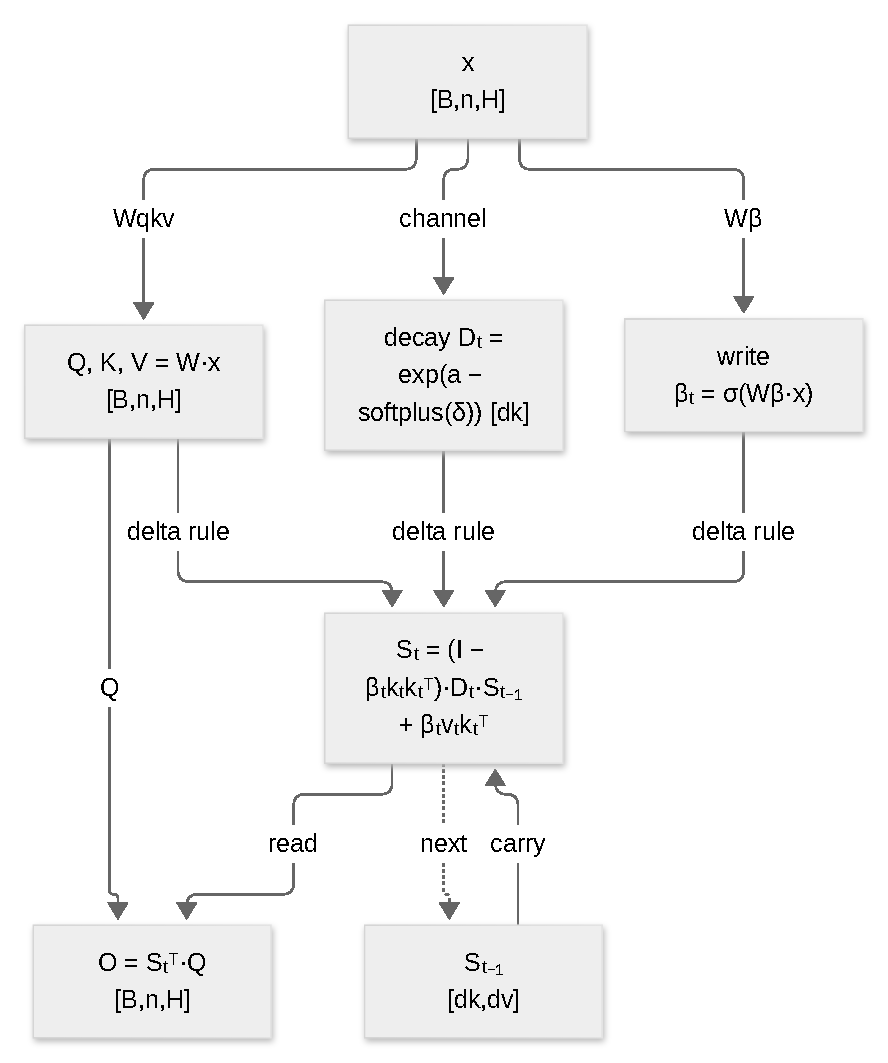
\includegraphics{../paper/figures/mixers/kda.pdf}}
\caption{Flujo de datos de KDA: el decaimiento por canal y una compuerta escalar de escritura modulan la actualización del estado por regla delta.}
\label{fig:mixer-kda}
\end{figure}

\subsubsection{Fundamento Matemático}

Kimi Delta Attention \citep{kimi_kda_2025} es el módulo central de Kimi Linear y extiende Gated DeltaNet con una \textbf{compuerta de decaimiento canalizada} de grano más fino. Mientras que Gated DeltaNet usa un único decaimiento escalar por cabeza $\alpha_t$ junto con la compuerta escalar de escritura delta $\beta_t$, KDA reemplaza el decaimiento escalar con un decaimiento \textbf{por canal de clave} $\boldsymbol{\alpha}_t \in \mathbb{R}^{d_k}$, parametrizado mediante una formulación de log-decaimiento y aplicado como una matriz diagonal $\mathbf{D}_t = \mathrm{diag}(\boldsymbol{\alpha}_t)$ antes de la actualización de la regla delta. La regla delta en sí retiene una compuerta de escritura escalar por cabeza $\beta_t$:
\[
\mathbf{S}_t = (\mathbf{I} - \beta_t \mathbf{k}_t \mathbf{k}_t^\top)\, \mathbf{D}_t\, \mathbf{S}_{t-1} + \beta_t \mathbf{v}_t \mathbf{k}_t^\top, \qquad \mathbf{o}_t = \mathbf{S}_t^\top \mathbf{q}_t
\]
El decaimiento canalizado sigue una parametrización de log-decaimiento (calculada en fp32 por estabilidad numérica en productos acumulativos largos):
\[
\mathbf{g} = \mathbf{a} - \mathrm{softplus}(\boldsymbol{\delta}), \qquad \boldsymbol{\alpha}_t = \exp(\mathbf{g})
\]
donde $\mathbf{a}$ y $\boldsymbol{\delta}$ son parámetros aprendidos por canal. Esto da a cada canal de clave una escala temporal de olvido independiente, permitiendo al modelo retener algunos canales más tiempo que otros dentro de la misma cabeza.

\paragraph{Reducción a Gated DeltaNet}: Cuando $\boldsymbol{\alpha}_t$ colapsa a un escalar (es decir, todos los canales comparten el mismo decaimiento), KDA se reduce exactamente a Gated DeltaNet. El decaimiento canalizado es por tanto una generalización estricta que añade selectividad por canal sobre el decaimiento/escritura escalares de Gated DeltaNet.

\paragraph{Entrenamiento por fragmentos}: Un algoritmo por fragmentos ad hoc usa una variante \textbf{Diagonal-Plus-Low-Rank (DPLR)} especializada de la matriz de transición para mantener la eficiencia en hardware. El producto de las transiciones por paso $(\mathbf{I} - \beta_t \mathbf{k}_t \mathbf{k}_t^\top)\mathbf{D}_t$ admite una descomposición DPLR que permite paralelismo rico en matmuls en tensor cores preservando la estructura de decaimiento canalizado.

\begin{algorithm}[H]
\caption{Avance Recurrente de Kimi Delta Attention (Forma de Referencia)}
\begin{algorithmic}[1]
\Require Entrada $\mathbf{x}_t$; estado previo $\mathbf{S}_{t-1} \in \mathbb{R}^{d_k \times d_v}$
\Require Proyecciones: $W_q, W_k, W_v, W_\beta$; parámetros de log-decaimiento $\mathbf{a}, \boldsymbol{\delta}$
\Ensure Salida $\mathbf{o}_t$ y estado $\mathbf{S}_t$
\State $\mathbf{q}_t \gets W_q \mathbf{x}_t$, $\mathbf{k}_t \gets W_k \mathbf{x}_t$, $\mathbf{v}_t \gets W_v \mathbf{x}_t$
\State $\beta_t \gets \mathrm{sigmoid}(W_\beta \mathbf{x}_t)$ \Comment{compuerta de escritura escalar por cabeza}
\State $\boldsymbol{\alpha}_t \gets \exp(\mathbf{a} - \mathrm{softplus}(\boldsymbol{\delta}))$ \Comment{decaimiento canalizado, fp32}
\State $\mathbf{D}_t \gets \mathrm{diag}(\boldsymbol{\alpha}_t)$ \Comment{matriz diagonal de decaimiento}
\State Decaer estado: $\mathbf{S}_t \gets \mathbf{D}_t \mathbf{S}_{t-1}$
\State Lectura: $\mathbf{r}_t \gets \mathbf{S}_t^\top \mathbf{k}_t$ \Comment{predicción actual a lo largo de la clave}
\State Actualización delta: $\mathbf{S}_t \gets \mathbf{S}_t - \beta_t \mathbf{k}_t \mathbf{r}_t^\top + \beta_t \mathbf{v}_t \mathbf{k}_t^\top$
\State Recuperar: $\mathbf{o}_t \gets \mathbf{S}_t^\top \mathbf{q}_t$
\State Compuerta de salida: $\mathbf{o}_t \gets \mathrm{GroupNorm}(\mathbf{o}_t) \odot \mathrm{silu}(W_g \mathbf{x}_t)$
\State \Return $\mathbf{o}_t$, $\mathbf{S}_t$
\end{algorithmic}
\end{algorithm}

\subsubsection{Rendimiento Empírico y Compromisos}

KDA está desplegado en Kimi Linear, un modelo híbrido (3B activados / 48B parámetros totales) que combina capas KDA con Multi-head Latent Attention (MLA). Kimi Linear supera a un baseline de MLA completa en todas las tareas evaluadas, reduce el caché KV hasta un $75\%$, y logra hasta $6\times$ de throughput de decodificación para contexto de 1M de tokens. El decaimiento canalizado es el principal impulsor de la ganancia: permite control fino sobre qué canales de clave persisten, mejorando el recuerdo de contexto largo frente a Gated DeltaNet con decaimiento escalar.

\begin{table}[H]
\centering
\footnotesize
\begin{tabularx}{\linewidth}{lXX}
\toprule
\textbf{Aspecto} & \textbf{Fortaleza} & \textbf{Limitación} \\
\midrule
Recuperación & El decaimiento canalizado mejora el recuerdo de contexto largo frente a baselines de decaimiento escalar; desplegado en Kimi Linear (híbrido 3B/48B). & El estado recurrente matricial $\mathcal{O}(d^2)$ es más pesado que la atención lineal con compuerta diagonal. \\
Rendimiento & Hasta $6\times$ de throughput de decodificación a 1M de contexto; $75\%$ de reducción de caché KV frente a MLA completa. & Requiere kernels por fragmentos conscientes de DPLR para eficiencia en hardware. \\
Memoria & Estado de inferencia constante $\mathcal{O}(d^2)$ (recurrente matricial). & El cálculo log-decaimiento en fp32 añade sobrecarga; la reducción a Gated DeltaNet pierde selectividad por canal. \\
\bottomrule
\end{tabularx}
\caption{Compromisos de KDA en Kimi Linear (3B activados / 48B total) \citep{kimi_kda_2025}.}
\label{tab:kda-tradeoffs-es}
\end{table}

\normalsize

\subsection{Principio Unificado de Compuerta}

Las ocho arquitecturas comparten un principio común: \textbf{la compuerta es un mecanismo para controlar el flujo de información y la retención selectiva de memoria}. Las decisiones de diseño específicas divergen a lo largo de varias dimensiones:

\begin{enumerate}[leftmargin=*]
    \item \textbf{Ubicación de la compuerta}: Actualizaciones de estado recurrente (GLA, DeltaNet, Gated DeltaNet, Gated DeltaNet-2, HGRN2) versus espacio de logits/salida softmax (FoX, Gated Softmax, RetNet).
    \item \textbf{Granularidad de control}: Por dimensión (GLA, HGRN2 diagonal), por clave (DeltaNet), por token (FoX), por cabeza (Gated Softmax) o borrado/escritura canalizados decouplados (Gated DeltaNet-2).
    \item \textbf{Dependencia de datos}: Completamente dependiente de datos (GLA, DeltaNet, Gated DeltaNet, Gated DeltaNet-2, FoX, Gated Softmax) versus esquemas fijos (RetNet con decaimiento exponencial).
    \item \textbf{Compensación de expresividad}: Eficiencia recurrente lineal (GLA, DeltaNet, Gated DeltaNet, Gated DeltaNet-2, HGRN2, RetNet) versus expresividad completa de softmax (FoX, Gated Softmax).
\end{enumerate}

\subsection{Implementación y Orientación Práctica}

\subsubsection{Cuándo Usar Cada Arquitectura}

\begin{enumerate}[leftmargin=*]
    \item \textbf{GLA}: Inferencia rápida con contextos moderados a largos (2K--20K tokens), cuando los kernels CUDA personalizados son aceptables y el rendimiento de recuperación no es crítico.
    \item \textbf{DeltaNet}: Fuerte recuperación asociativa y tareas de aprendizaje en contexto; bueno para tareas sintéticas (MQAR) y pruebas de asociación clave-valor.
    \item \textbf{Gated DeltaNet}: Modelos de producción que requieren el mejor equilibrio de recuperación, olvido y rendimiento (probado en Qwen3-Next; ICLR 2025).
    \item \textbf{Gated DeltaNet-2}: Cargas de recuperación de contexto largo (multi-key NIAH) donde el borrado/escritura canalizado decouplado da el recuerdo más fuerte; cuando se dispone de un kernel WY consciente de las compuertas.
    \item \textbf{RetNet}: Inferencia extremadamente eficiente sin almacenamiento en caché KV; adecuado para despliegues en dispositivos móviles/de borde o modelos de juguete.
    \item \textbf{HGRN2}: Jerarquías temporales multi-escala; cuando los límites de olvido específicos por capa son deseables.
    \item \textbf{FoX}: Extrapolación de longitud y comprensión de contexto largo; cuando el entrenamiento cuadrático es aceptable y no se desea reemplazar softmax.
    \item \textbf{Gated Softmax}: Mejora rápida para modelos softmax existentes con cambios mínimos de código; mejor para profesionales que desean ganancias inmediatas sin una reestructuración importante.
\end{enumerate}

\subsubsection{Consideraciones de Hardware}

\begin{table}[H]
\centering
\small
\begin{tabularx}{0.95\linewidth}{Xp{3.5cm}p{3.5cm}}
\toprule
\textbf{Objetivo de Hardware} & \textbf{Arquitecturas Recomendadas} & \textbf{Notas} \\
\midrule
GPU (H100/A100) & Gated Softmax, FoX, Gated DeltaNet, Gated DeltaNet-2 & Implementaciones maduras de softmax/lineal. GLA/DeltaNet requieren kernels personalizados. \\
TPU (alta memoria) & GLA, DeltaNet, Gated DeltaNet, Gated DeltaNet-2, HGRN2 & Hardware soporta matmuls eficientes; los métodos recurrentes lineales brillan. \\
Móvil/Borde & RetNet, Gated Softmax ligero & Inferencia con memoria constante es crítica. \\
\bottomrule
\end{tabularx}
\end{table}


\section{Normalización, Cuantización, Enrutamiento de Profundidad y Algoritmos de Ejecución}
\label{sec:annex-norm-bitnet-mod}

Este anexo recopila el detalle a nivel de implementación para las variantes de normalización, cuantización ternaria estilo BitNet, enrutamiento adaptativo de profundidad (Mixture-of-Depths), memoria condicional (Engram), embeddings factorizados y los algoritmos de ejecución (controles de estabilidad del paso de entrenamiento, enrutador de inferencia SBERT) que soportan la tubería impulsada por configuración. (Las conexiones residuales restringidas por variedad de mHC se documentan por separado en el Anexo~9.) Las secciones principales difieren a este anexo para las formulaciones matemáticas y el pseudocódigo; las claves bibliográficas citadas aquí se resuelven contra \texttt{docs/bibliography/}.

\subsection{Variantes de Normalización: LayerNorm, RMSNorm, pRMSNorm, Tanh Dinámico, Erf Dinámico y FlashNorm}

La normalización determina cómo se controla la escala de activación a través de la profundidad. En este repositorio, la normalización no es solo una elección de modelado sino también una cuestión de compatibilidad con el esquema, porque solo ciertos valores son actualmente aceptados por \texttt{norm\_type}. El contrato del esquema es:
\[
\texttt{norm\_type} \in \{\texttt{layer\_norm}, \texttt{dynamic\_tanh}, \texttt{derf}, \texttt{rms\_norm}, \texttt{prms\_norm}, \texttt{flash\_norm}\}
\]
Las formulaciones más relevantes para este código base son:

\subsubsection{LayerNorm (Línea Base)}
LayerNorm \citep{ba2016layer} es el normalizador por defecto; centra y reescala cada token por su media y varianza por token:
\[
\mu = \frac{1}{d}\sum_{i=1}^{d} x_i, \quad \sigma^2 = \frac{1}{d}\sum_{i=1}^{d}(x_i - \mu)^2, \quad y_i = \gamma_i \frac{x_i - \mu}{\sqrt{\sigma^2 + \epsilon}} + \beta_i.
\]

\subsubsection{RMSNorm}
RMSNorm elimina la centralización de la media y solo reescala por la magnitud de la raíz cuadrada media \citep{zhang_root_2019}:
\[
\mathrm{RMS}(x)=\sqrt{\frac{1}{d}\sum_{i=1}^{d}x_i^2+\epsilon},\qquad
y_i=\gamma_i\frac{x_i}{\mathrm{RMS}(x)}.
\]
En comparación con LayerNorm, RMSNorm es computacionalmente más simple (sin resta de la media de características) y se usa a menudo cuando es importante reducir la sobrecarga de normalización (p.\,ej., Llama, GPT-NeoX). Tiene una escala $\gamma$ aprendible por dimensión pero sin término de bias.

\subsubsection{RMSNorm Parcial (pRMSNorm)}
pRMSNorm \citep{zhang_root_2019} reduce aún más la sobrecarga estimando el RMS de solo el primer $p$\% de las dimensiones ocultas:
\[
\mathrm{RMS}(x)=\sqrt{\frac{1}{k}\sum_{i=1}^{k}x_i^2+\epsilon},\qquad k=\lceil d\cdot p\rceil,
\]
explotando el supuesto de que las neuronas dentro de una capa son aproximadamente i.i.d. La misma escala $\gamma$ se aplica a todas las dimensiones. La razón parcial $p$ se controla mediante el campo de configuración \texttt{prms\_partial\_ratio} (por defecto $6.25\%$). El paper reporta que se pueden lograr resultados competitivos con tan solo el $6.25\%$ de las entradas, aunque puede surgir inestabilidad de gradiente con razones muy pequeñas.

\subsubsection{Tanh Dinámico (DyT)}
El Tanh Dinámico propone reemplazar la normalización explícita con un mapeo elemento a elemento acotado \citep{zhu_transformers_2025}:
\[
\mathrm{DyT}(x)=\tanh(\alpha x)
\]
donde $\alpha$ se aprende. La idea central es que la contracción no lineal acotada puede proporcionar un escalado de señal estable sin calcular explícitamente estadísticas de normalización por token.

\subsubsection{Erf Dinámico (Derf)}
Derf extiende la misma dirección libre de normalización usando un mapeo basado en la función error \citep{chen_stronger_2025}:
\[
\mathrm{Derf}(x)=\mathrm{erf}(\alpha x+s)
\]
con escala/desplazamiento aprendibles. Los resultados reportados en el trabajo citado indican un rendimiento superior al de DyT y las líneas base de normalización comunes en múltiples dominios.

\subsubsection{FlashNorm (RMSNorm sin pesos)}
FlashNorm \citep{graef2026flashnorm} no es una nueva normalización matemática; es una \emph{reescritura algebraica exacta} del ubicuo par ``$\mathrm{RMSNorm} \to \mathrm{Lineal}$'' que (i) elimina la escala aprendible por dimensión $\mathbf{g}$ al plegarla en los pesos de la capa lineal subsecuente, y (ii) difiere la reducción escalar RMS a la salida de la multiplicación matricial, de modo que el \texttt{matmul} (unidad matricial) y la reducción RMS (unidad vectorial) se ejecuten en paralelo. Tres proposiciones formalizan la reescritura.

\paragraph{Proposición 1 (Plegado de pesos).}
Dada la activación $\mathbf{a}\in\mathbb{R}^{n}$, el peso RMSNorm $\mathbf{g}\in\mathbb{R}^{n}$ y una lineal subsecuente $\mathbf{W}\in\mathbb{R}^{n\times k}$,
\[
\mathbf{z}=\mathrm{RMSNorm}(\mathbf{a})\mathbf{W}=\frac{\mathbf{a}}{\mathrm{RMS}(\mathbf{a})}\mathbf{W}^{*},\qquad
W^{*}_{i,j}=g_{i}\cdot W_{i,j}\ \Leftrightarrow\ \mathbf{W}^{*}=\operatorname{diag}(\mathbf{g})\mathbf{W}.
\]
La escala por dimensión $\mathbf{g}$ se vuelve redundante y se pliega en $\mathbf{W}$ una única vez al cargar el modelo. El módulo autónomo \texttt{FlashNorm} de este repositorio aplica esto directamente: \emph{no tiene parámetros aprendibles} (la escala está destinada a ser absorbida por la proyección subsecuente).

\paragraph{Proposición 2 (Normalización diferida).}
Para una lineal sin bias $\mathbf{W}^{*}$, la conmutatividad escalar--matricial produce
\[
\frac{\mathbf{a}}{\mathrm{RMS}(\mathbf{a})}\mathbf{W}^{*}=\left(\mathbf{a}\mathbf{W}^{*}\right)\cdot\frac{1}{\mathrm{RMS}(\mathbf{a})}.
\]
El \texttt{matmul} $\mathbf{a}\mathbf{W}^{*}$ y la reducción RMS son independientes entre sí; en hardware con unidades matriciales y vectoriales diferenciadas se ejecutan en paralelo, y solo una multiplicación vectorial--escalar los sincroniza. El módulo fusionado \texttt{FlashNormLinear} implementa esta reescritura: en la ruta sin bias calcula el \texttt{matmul} sobre la entrada \emph{no normalizada} y multiplica el resultado por el RMS recíproco por token. Cuando la lineal tiene bias $\mathbf{c}$, la reescritura deja de ser exacta (Observación 1 del paper): $\left(\mathbf{a}\mathbf{W}^{*}+\mathbf{c}\right)/\mathrm{RMS}(\mathbf{a})\neq\mathbf{a}\mathbf{W}^{*}/\mathrm{RMS}(\mathbf{a})+\mathbf{c}$; la capa entonces aplica el escalar a la entrada primero y deja que la lineal añada su bias como de costumbre.

\paragraph{Proposición 3 (Cancelación de RMS).}
Por la invariancia de escala de RMS, $\mathrm{RMS}(\alpha\mathbf{a})=\alpha\,\mathrm{RMS}(\mathbf{a})$. Por tanto, un patrón ``$\mathrm{RMSNorm}\to\mathrm{Lineal}\to\mathrm{RMSNorm}$'' permite que el \emph{primer} RMSNorm se elimine por completo:
\[
\mathrm{RMSNorm}\!\left(\frac{\mathbf{a}}{\mathrm{RMS}(\mathbf{a})}\mathbf{W}^{*}\right)=\mathrm{RMSNorm}\!\left(\mathbf{a}\mathbf{W}^{*}\right).
\]
Esta cancelación es relevante para la normalización QKV (Gemma~4) y la normalización latente MLA (DeepSeek-V2, Mistral Small~4); no se aplica automáticamente en este repositorio pero se documenta por completitud.

\paragraph{Composición con RMS parcial.}
FlashNorm se compone naturalmente con el truco pRMSNorm (§\ref{sec:annex-norm-bitnet-mod}, subsección pRMSNorm): cuando \texttt{flashnorm\_partial\_ratio} $=p>0$, el RMS se estima solo de los primeros $k=\lceil d\cdot p\rceil$ elementos de la entrada, reduciendo aún más el costo de la reducción RMS en la unidad vectorial.

\paragraph{Interacción con BitNet.}
Plegar un $\mathbf{g}$ de coma flotante en el tensor de pesos ternarios de BitNet $\{-1,0,+1\}$ \citep{wang_bitnet_2023} destruiría la cuantización, y BitLinear aplica su propio LayerNorm interno antes de la cuantización de activaciones, el cual necesita la entrada normalizada. El módulo fusionado \texttt{FlashNormBitLinear} por tanto recurre a la composición secuencial $\mathrm{FlashNorm}\to\mathrm{BitLinear}$: el \texttt{matmul} y la reducción RMS aún se ejecutan en paralelo, pero la multiplicación escalar post-\texttt{matmul} de la Prop.~2 se sacrifica. El plegado de $\mathbf{g}$ en coma flotante en un tensor de pesos de 1.58 bits se deja a trabajo futuro a nivel kernel.

\paragraph{Pseudocódigo PyTorch.}
\begin{algorithmic}[1]
\State \textbf{Entrada:} activación $\mathbf{a}\in\mathbb{R}^{T\times n}$, peso RMSNorm $\mathbf{g}\in\mathbb{R}^{n}$, lineal $\mathbf{W}\in\mathbb{R}^{n\times k}$, bias $\mathbf{c}\in\mathbb{R}^{k}$ o \texttt{None}
\State \texttt{// Prop. 1: plegado de pesos al cargar}
\State $\mathbf{W}^{*}\gets \mathbf{g}\odot\mathbf{W}$ \Comment{por columnas; \texttt{g.unsqueeze(0) * W} en PyTorch}
\State $\mathbf{g}\gets \mathbf{1}$ \Comment{la norma autónoma ahora es sin pesos}
\State \texttt{// Prop. 2: paso forward con RMS diferida (ruta sin bias)}
\State $\mathbf{b}\gets \mathbf{a}\mathbf{W}^{*\top}$ \Comment{unidad matricial / tensor cores}
\State $\mathrm{rms\_inv}\gets \mathrm{rsqrt}(\mathrm{mean}(\mathbf{a}^{2})+\varepsilon)$ \Comment{unidad vectorial, independiente de $\mathbf{b}$}
\If{$\mathbf{c}=\texttt{None}$}
    \State \textbf{retornar} $\mathbf{b}\cdot\mathrm{rms\_inv}$ \Comment{una sola multiplicación vectorial--escalar}
\Else
    \State \texttt{// Obs. 1: ruta con bias secuencial; matmul/RMS paralelizan}
    \State \textbf{retornar} $(\mathbf{a}\cdot\mathrm{rms\_inv})\mathbf{W}^{*\top}+\mathbf{c}$
\EndIf
\end{algorithmic}

\paragraph{Latencia reportada (GPU NVIDIA T4).}
El paper reporta las siguientes aceleraciones sobre la operación \emph{norm-then-project}, con un despacho adaptativo que cae al camino secuencial en el régión limitada por memoria (decodificación):

\scriptsize
\begin{tabular}{llrrrl}
\toprule
\textbf{Escala} & \textbf{Tokens} & \textbf{Secuencial (ms)} & \textbf{FlashNorm (ms)} & \textbf{Aceleración} & \textbf{Notas} \\
\midrule
SmolLM2-135M & 4096 & 0.704 & 0.468 & $+33.6\%$ & limitada por cómputo (prefill) \\
SmolLM2-135M & 8192 & 0.929 & 0.599 & $+35.5\%$ & limitada por cómputo (prefill) \\
Llama-7B     & 1024 & 1.882 & 1.654 & $+12.1\%$ & limitada por cómputo (prefill) \\
Llama-7B     & 4096 & 7.628 & 6.570 & $+13.9\%$ & limitada por cómputo (prefill) \\
\bottomrule
\end{tabular}
\normalsize

\paragraph{Validación de plegado sin pérdida.}
El plegado de pesos (Prop.~1) es matemáticamente exacto; el paper verificó salidas bit-idénticas en tres checkpoints abiertos:

\scriptsize
\begin{tabular}{lll}
\toprule
\textbf{Modelo} & \textbf{Precisión} & \textbf{Resultado} \\
\midrule
SmolLM2-135M & fp16 & diff máxima $=0.0$, similitud coseno $=1.0$, texto idéntico \\
Llama-3.2-1B & fp32 & generación voraz bit-idéntica \\
Llama-3.1-8B & fp32 & generación voraz bit-idéntica \\
\bottomrule
\end{tabular}
\normalsize
La preservación de calidad en \texttt{lm-evaluation-harness} (wikitext word\_ppl, MMLU 5-shot, HellaSwag 0-shot) se mantiene dentro del ruido del benchmark (peor $\Delta=+0.0017$ word\_ppl).

\subsubsection{Comparación}
\scriptsize
\begin{longtable}{L{2.2cm}L{3.4cm}L{2.0cm}L{4.0cm}}
\toprule
\textbf{Método} & \textbf{Fórmula} & \textbf{Estadísticas Necesarias} & \textbf{Notas} \\
\midrule
\endhead
LayerNorm & $\gamma_i (x_i - \mu)/\sqrt{\sigma^2 + \epsilon} + \beta_i$ & media + varianza & Por defecto; centrado y reescalado completo \citep{ba2016layer}. \\
RMSNorm & $\gamma_i x_i/\sqrt{\frac{1}{d}\sum_j x_j^2+\epsilon}$ & Solo RMS & Menor sobrecarga; línea base ampliamente usada \citep{zhang_root_2019}. \\
pRMSNorm & $\gamma_i x_i/\sqrt{\frac{1}{k}\sum_{j\le k} x_j^2+\epsilon}$ & RMS parcial & RMS del primer $p$\% de dims; \texttt{prms\_partial\_ratio} por defecto $6.25\%$ \citep{zhang_root_2019}. \\
Tanh Dinámico & $\tanh(\alpha x)$ & ninguna & Transformación acotada libre de normalización; reemplazo directo \citep{zhu_transformers_2025}. \\
Erf Dinámico & $\mathrm{erf}(\alpha x+s)$ & ninguna & Alternativa libre de normalización; mejora sobre DyT \citep{chen_stronger_2025}. \\
FlashNorm & $x_i/\sqrt{\frac{1}{d}\sum_j x_j^2+\epsilon}$ (sin pesos) & Solo RMS & Reescritura exacta de RMSNorm$\to$Lineal: pliega $\mathbf{g}$ en $\mathbf{W}$ (Prop.~1), difiere el escalar RMS a la salida del \texttt{matmul} (Prop.~2); 12--35\% de reducción de latencia en GPU T4 \citep{graef2026flashnorm}. \\
\bottomrule
\end{longtable}
\normalsize

\subsection{Ruta de Cuantización Ternaria BitNet}

Cuando \texttt{use\_bitnet=true}, las capas BitLinear reemplazan a \texttt{nn.Linear} estándar con cuantización ternaria de pesos ($-1, 0, +1$) siguiendo BitNet \citep{wang_bitnet_2023}. Dado el tensor de pesos $W$, un escalado práctico es:
\[
s=\text{mean}(|W|),\qquad
\tilde{W}=\text{clip}\left(\text{round}\left(\frac{W}{s}\right),-1,1\right).
\]
El mapeo empaquetado utiliza dos bits por símbolo de peso para eficiencia de almacenamiento. Esto permite una compresión significativa ($\sim 32\times$ frente a FP32) pero es experimental y puede afectar la calidad del modelo; es más adecuado para el despliegue de inferencia.

La cuantización de activaciones para la ruta INT8 es:
\[
q=\text{round}\left(x\cdot\frac{127}{\max(|x|)+\epsilon}\right),\qquad q\in[-128,127]
\]
con des-cuantización $x\approx q/\alpha$. Para $N$ parámetros, las estimaciones de tamaño antes de metadatos y sobrecarga de empaquetado son:
\[
\text{Tamaño FP32}\approx 4N,\quad \text{Tamaño FP16}\approx 2N,\quad \text{Tamaño 1.58-bit}\approx \frac{1.58}{8}N
\]
lo que se alinea con objetivos de despliegue ligero \citep{samson_lightweight_2026,bravin_embbert_2026}.

\subsection{Enrutamiento de Tokens Mixture-of-Depths (MoD)}

Cuando \texttt{use\_mixture\_of\_depths=true}, cada bloque del transformer puntúa los tokens con un enrutador ligero. Solo el subconjunto superior de \texttt{mixture\_of\_depths\_capacity\_ratio} se actualiza; los tokens omitidos pasan sin cambios \citep{zhu2026mixtureofdepthsattention}. Esto asigna más profundidad a los tokens destacados, reduciendo el cómputo por capa.

\begin{algorithmic}[1]
\State \textbf{Entrada:} estados ocultos $H \in \mathbb{R}^{n \times d}$, enrutador $R$, ratio de capacidad $\rho$
\State $\text{puntajes} \gets R(H)$ \Comment{puntaje del enrutador por token}
\State $\mathcal{S} \gets \texttt{top-k}(\text{puntajes}, k=\lceil \rho \cdot n \rceil)$ \Comment{seleccionar subconjunto destacado}
\State $H_{\text{actualizar}} \gets \texttt{bloque}(H[\mathcal{S}])$ \Comment{aplicar bloque transformer a tokens seleccionados}
\State $H[\mathcal{S}] \gets H_{\text{actualizar}}$ \Comment{escribir de vuelta; los tokens no seleccionados bypassan el bloque}
\State \textbf{Salida:} $H$ \Comment{pérdida auxiliar de balance de carga añadida desde \texttt{mixture\_of\_depths\_router\_aux\_loss\_weight}}
\end{algorithmic}

\subsubsection{Configuración}
\begin{itemize}[leftmargin=*]
    \item \texttt{use\_mixture\_of\_depths}: bool --- habilitar enrutamiento MoD de tokens.
    \item \texttt{mixture\_of\_depths\_capacity\_ratio}: float en $(0, 1]$ --- fracción de tokens actualizados por capa.
    \item \texttt{mixture\_of\_depths\_router\_aux\_loss\_weight}: float $\ge 0$ --- peso de pérdida auxiliar para regularización del enrutador.
\end{itemize}

\subsection{Memoria Condicional Engram}

\begin{figure}[H]
\centering
\fitfigure{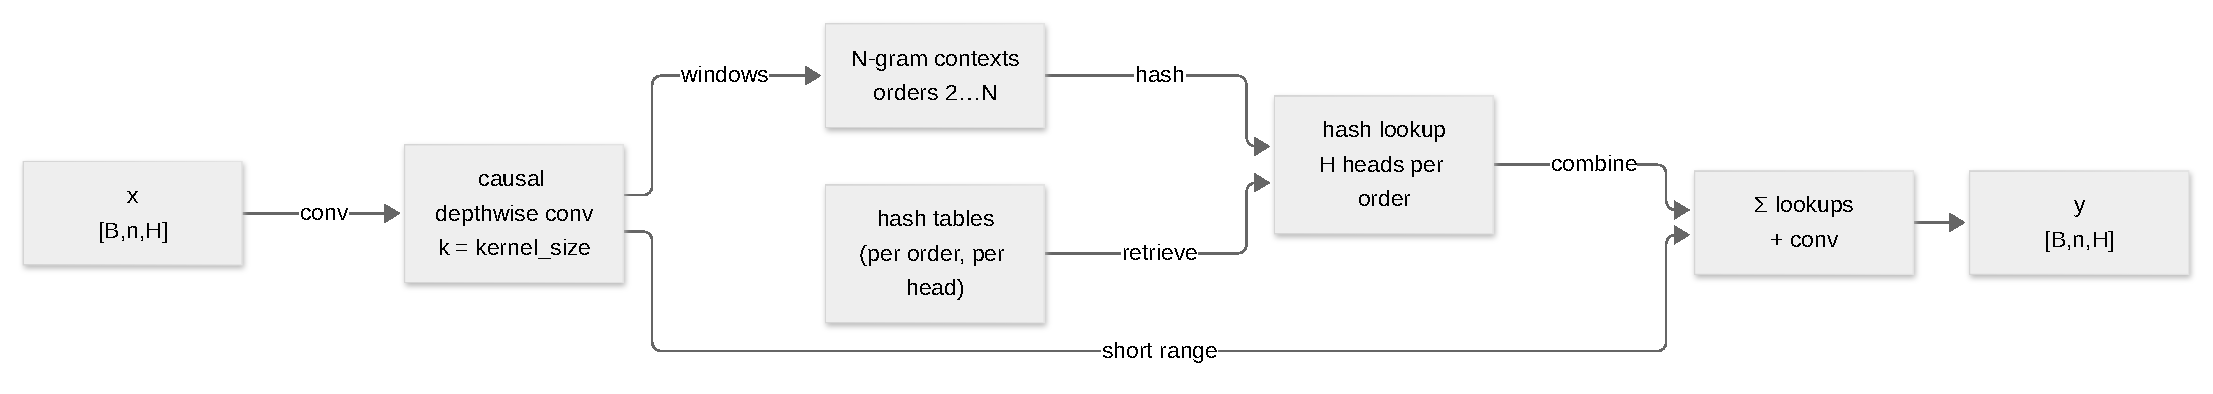
\includegraphics{../paper/figures/mixers/engram.pdf}}
\caption{Flujo de datos de la memoria condicional de Engram: una convolución causal depthwise aporta contexto de corto alcance, las búsquedas hash de N-gramas recuperan embeddings por orden, y las búsquedas se suman a la salida de la convolución.}
\label{fig:mixer-engram}
\end{figure}

Engram (\texttt{engram\_attn}) implementa memoria condicional mediante búsqueda N-gram escalable \citep{cheng2026conditionalmemoryscalablelookup}. Construye tablas de búsqueda basadas en hash para contextos N-gram desde tamaño 2 hasta \texttt{engram\_max\_ngram\_size}, con cabezas hash independientes por orden N-gram. Una convolución causal depthwise (\texttt{engram\_kernel\_size}) proporciona contexto de corto alcance antes de la búsqueda N-gram.

\begin{algorithmic}[1]
\State \textbf{Entrada:} flujo de tokens $x_{1:n}$, órdenes N-gram $\{2, \ldots, N\}$, cabezas hash por orden $H$
\State $h_{\text{conv}} \gets \text{DepthwiseConv1d}(x_{1:n}, k=\texttt{engram\_kernel\_size})$ \Comment{contexto de corto alcance}
\For{cada orden N-gram $k \in \{2, \ldots, N\}$}
    \State $\text{ctx}_t^{(k)} \gets x_{t-k+1:t}$ \Comment{ventana de contexto N-gram}
    \State $\text{lookup}^{(k)}_t \gets \text{HashTable}^{(k)}[\text{hash}(\text{ctx}_t^{(k)})]$ \Comment{recuperación por cabeza, $H$ cabezas por orden}
\EndFor
\State $y_t \gets \sum_{k} \text{lookup}^{(k)}_t + h_{\text{conv},t}$ \Comment{combinar memorias condicionales}
\State \textbf{Salida:} $y_{1:n}$
\end{algorithmic}

\subsubsection{Configuración}
\begin{itemize}[leftmargin=*]
    \item \texttt{engram\_max\_ngram\_size}: int $\ge 2$ --- orden N-gram más alto (por defecto 3).
    \item \texttt{engram\_n\_heads\_per\_ngram}: int $\ge 1$ --- cabezas hash por orden N-gram (por defecto 4).
    \item \texttt{engram\_embed\_dim\_per\_head}: int $\ge 1$ --- dimensión de embedding por cabeza hash (por defecto 32).
    \item \texttt{engram\_kernel\_size}: int $\ge 1$ --- ancho del kernel de conv causal depthwise (por defecto 4).
    \item \texttt{engram\_seed}: int --- semilla hash para reproducibilidad (por defecto 42).
\end{itemize}
Tamaño oculto total de Engram = $(\texttt{max\_ngram\_size} - 1) \times \texttt{n\_heads\_per\_ngram} \times \texttt{embed\_dim\_per\_head}$.

\subsection{Embeddings Factorizados y Convolución de Embedding}

\subsubsection{Embeddings Factorizados}
Cuando \texttt{use\_factorized\_embedding=true}, la matriz de embedding se factoriza en dos matrices más pequeñas, reduciendo parámetros de $O(V \times H)$ a $O(V \times R + R \times H)$ donde $R = \texttt{factorized\_embedding\_dim}$.
\begin{itemize}[leftmargin=*]
    \item \texttt{use\_factorized\_embedding}: bool --- habilitar factorización.
    \item \texttt{factorized\_embedding\_dim}: int $\ge 1$ --- dimensión intermedia (típico: 64--256).
\end{itemize}

\subsubsection{Convolución de Embedding}
Cuando \texttt{use\_embedding\_conv=true}, se aplica una Conv1d depthwise sobre el flujo de embeddings antes del primer bloque transformer, con tamaño de kernel \texttt{embedding\_conv\_kernel}. Esto proporciona un filtro ligero de contexto local sobre embeddings de tokens.

\subsection{Controles de Estabilidad del Paso de Entrenamiento}

El paso de entrenamiento guiado por esquema aplica acumulación de gradientes, recorte de norma global, guardas de explosión post-recorte y reintentos acotados de NaN/Inf. El gradiente acumulado es:
\[
g_{\text{acc}}=\frac{1}{K}\sum_{i=1}^{K} g_i,\quad K=\texttt{gradient\_accumulation\_steps}
\]
\[
g_{\text{clip}} = g_{\text{acc}}\cdot
\min\left(1,\frac{\tau}{\|g_{\text{acc}}\|_2+\epsilon}\right),\quad
\tau=\texttt{grad\_clip\_max\_norm}
\]
luego los guardas de desbordamiento usan \texttt{inf\_post\_clip\_threshold} y lógica de reintentos limitada por \texttt{max\_nan\_retries}.

\begin{algorithm}[t]
\caption{Paso de Entrenamiento Guiado por Esquema con Controles de Estabilidad}
\begin{algorithmic}[1]
\Require Flujo de lotes, configuración $C$
\State Inicializar contador de reintentos $r\gets 0$
\For{cada paso del optimizador}
    \State Acumular gradientes para $K=C.\texttt{gradient\_accumulation\_steps}$ micro-lotes
    \State Aplicar recorte de norma global con $\tau=C.\texttt{grad\_clip\_max\_norm}$
    \If{el gradiente post-recorte excede $C.\texttt{inf\_post\_clip\_threshold}$ o se detecta NaN/Inf}
        \If{$r < C.\texttt{max\_nan\_retries}$}
            \State restaurar estado seguro / saltar paso; $r \gets r+1$
            \State \textbf{continue}
        \Else
            \State detener entrenamiento con estado de fallo
        \EndIf
    \EndIf
    \State ejecutar paso del optimizador seleccionado por \texttt{optimizer\_class}
    \State actualizar scheduler (\texttt{cosine}, \texttt{constant}, o \texttt{linear\_warmup\_then\_constant})
    \If{paso mod \texttt{checkpoint\_every\_n\_steps}$=0$}
        \State guardar checkpoint rodante y podar a \texttt{max\_rolling\_checkpoints}
    \EndIf
    \State actualizar mejores checkpoints hasta \texttt{num\_best\_checkpoints}
    \State emitir CSV + telemetría según \texttt{gradient\_log\_interval} y \texttt{telemetry\_log\_interval}
\EndFor
\end{algorithmic}
\end{algorithm}

\subsection{Partición de Test Reservada y Evaluación al Final del Entrenamiento}

\texttt{training.test\_percentage} reserva una fracción determinista del dataset de la tarea antes del primer paso del optimizador. Con $n$ ejemplos, porcentaje reservado $\rho=\texttt{test\_percentage}/100$ y una permutación $\pi$ sorteada una sola vez con semilla fija, la partición es
\[
n_{\text{test}}=\operatorname{clip}\!\left(\operatorname{round}(\rho n),\,1,\,n-1\right),\qquad
\mathcal{D}_{\text{train}}=\{x_{\pi(i)}\}_{i=n_{\text{test}}+1}^{n},\qquad
\mathcal{D}_{\text{test}}=\{x_{\pi(i)}\}_{i=1}^{n_{\text{test}}} ,
\]
de modo que la misma configuración siempre reserva los mismos ejemplos, sea cual sea el mezclado del DataLoader. Tras la última época se evalúan los pesos finales una vez con el objetivo de la tarea bajo \texttt{no\_grad}, y la pérdida y precisión ponderadas por muestra
\[
\hat{L}=\frac{1}{n_{\text{test}}}\sum_{x\in\mathcal{D}_{\text{test}}}\ell(f_\theta;x),\qquad
\widehat{\text{acc}}=\frac{1}{n_{\text{test}}}\sum_{x\in\mathcal{D}_{\text{test}}}a(f_\theta;x)
\]
se escriben en \texttt{test\_metrics.json} junto al log CSV. La partición cubre modelado de lenguaje enmascarado y causal, clasificación de texto, las tres tareas de visión, ASR (donde el campo de precisión lleva la tasa de error de caracteres, etiquetada \texttt{metric: cer}) y clasificación de audio. SBERT conserva su propia partición de validación mediante \texttt{training.sbert.max\_eval\_samples} y no se ve afectado. Fijar el campo en cero desactiva la partición y restaura el comportamiento histórico sobre todos los datos.

\subsection{Enrutador de Modo de Inferencia SBERT}

El despachador de inferencia SBERT selecciona entre puntuación de similitud, búsqueda sobre corpus, agrupamiento y codificación persistente sobre un único codificador compartido \citep{reimers_sentence-bert_2019}. La similitud coseno y la pérdida de regresión son:
\[
\text{cos}(e_1,e_2)=\frac{e_1^\top e_2}{\|e_1\|\|e_2\|},\qquad
\mathcal{L}_{\text{cos}}=\left(\text{cos}(e_1,e_2)-y\right)^2
\]
con $y\in[-1,1]$ en este pipeline.

\begin{algorithm}[t]
\caption{Enrutador de Modo de Inferencia SBERT}
\begin{algorithmic}[1]
\Require modo $m$, modelo $E$, entradas $X$
\If{$m=\texttt{similarity}$}
    \State retornar $\cos(E(x_1),E(x_2))$
\ElsIf{$m=\texttt{search}$}
    \State retornar top-$k$ por producto-punto/coseno contra embeddings del corpus
\ElsIf{$m=\texttt{cluster}$}
    \State retornar etiquetas de clustering sobre $E(X)$
\Else
    \State retornar embeddings serializados $E(X)$
\EndIf
\end{algorithmic}
\end{algorithm}
\section{Funciones de Activación}
\label{sec:annex-funciones-activacion}

Este anexo documenta la librería completa de funciones de activación
disponibles en el modelo. La librería proporciona \textbf{43 funciones de
activación feed-forward}: 40 activaciones elementales y 3 variantes de FFN con
compuerta. Las activaciones se agrupan en cinco familias, siguiendo la
taxonomía de Dubey et al.~\citep{dubey2021activations} y la visión analítica de
Lederer~\citep{lederer2021activations}, y se añade la \emph{Rational Activation
Function} (RAF) aprendible de Fang et al.~\citep{fang2023raft}.

La selección se controla mediante el campo de configuración
\texttt{ffn\_activation} (un enumerado de cadenas) y se despacha en tiempo de
ejecución mediante una factoría que replica el patrón de las capas de
normalización (Anexo~7).

\[
\texttt{ffn\_activation} \in \{\texttt{silu},\;\texttt{gelu},\;\dots,\;
\texttt{raf},\;\texttt{swiglu},\;\texttt{geglu},\;\texttt{reglu}\}
\]

\subsection{Familia Clásica / Sigmoid--Tanh (12 activaciones)}

La familia clásica comprende activaciones suaves, sin estado, basadas en
funciones logísticas y algebraicas~\citep{lederer2021activations,dubey2021activations}.
Todas comparten monotonicía o casi-monotonicía y son continuamente derivables.

{\footnotesize
\begin{align}
  \text{Sigmoid}(x) &= \frac{1}{1+e^{-x}}
    & \text{Rango: } (0,1),\;\text{monótona, suave}
    & \quad \text{\citep{lederer2021activations}} \\[4pt]
  \text{Tanh}(x) &= \frac{e^{x}-e^{-x}}{e^{x}+e^{-x}} = 2\,\sigma(2x)-1
    & \text{Rango: } (-1,1),\;\text{monótona, suave}
    & \quad \text{\citep{lederer2021activations}} \\[4pt]
  \text{Arctan}(x) &= \arctan(x)
    & \text{Rango: } (-\tfrac{\pi}{2},\tfrac{\pi}{2}),\;\text{monótona, suave}
    & \quad \text{\citep{lederer2021activations}} \\[4pt]
  \text{Softsign}(x) &= \frac{x}{1+|x|}
    & \text{Rango: } (-1,1),\;\text{suave, deriv.\ una vez en 0}
    & \quad \text{\citep{lederer2021activations}} \\[4pt]
  \text{Elliott}(x) &= \frac{x}{1+|x|}
    & \text{Alias de Softsign (notación ``elliottsig'' del survey)}
    & \quad \text{\citep{lederer2021activations}} \\[4pt]
  \text{Identity}(x) &= x
    & \text{Rango: } (-\infty,\infty),\;\text{lineal, }C^\infty
    & \quad \text{(interna)}
\end{align}
}  % end size group

{\scriptsize
\begin{align}
  \text{Softplus}(x) &= \log(1+e^{x})
    & \text{Rango: } [0,\infty),\;\text{suave, }C^\infty
    & \quad \text{\citep{glorot2011softplus}} \\[4pt]
  \text{Mish}(x) &= x\,\tanh\!\big(\text{softplus}(x)\big)
    = x\,\tanh\!\big(\log(1+e^{x})\big)
    & \text{Rango: } [\approx{-0.31},\infty),\;\text{no monótona, suave}
    & \quad \text{\citep{misra2019mish}} \\[4pt]
  \text{GELU}(x) &= x\,\Phi(x) = x\cdot\tfrac{1}{2}\Big(1+\text{erf}\!\Big(\frac{x}{\sqrt{2}}\Big)\Big)
    & \text{Rango: } (\approx{-0.17},\infty),\;\text{suave, probabilística}
    & \quad \text{\citep{hendrycks2016gelu}} \\[4pt]
  \text{GELU-tanh}(x) &= \tfrac{x}{2}\Big(1+\tanh\!\Big(\sqrt{\tfrac{2}{\pi}}
    (x+0.044715\,x^{3})\Big)\Big)
    & \text{Aproximación con tanh de GELU (más rápida)}
    & \quad \text{\citep{hendrycks2016gelu}} \\[4pt]
  \text{ReLU}(x) &= \max(0,x)
    & \text{Rango: } [0,\infty),\;\text{tramos lineales, no suave en 0}
    & \quad \text{\citep{nair2010relu}} \\[4pt]
  \text{SiLU}(x) &= x\,\sigma(x) = \frac{x}{1+e^{-x}}
    & \text{Rango: } (\approx{-0.278},\infty),\;\text{no monótona, suave}
    & \quad \text{\citep{elfwing2018silu}}
\end{align}
}  % end size group

\noindent\textbf{SiLU} (Sigmoid Linear Unit) es la activación por defecto
(\texttt{ffn\_activation=silu}). Cuando $\beta=1$, el Swish paramétrico se
reduce a SiLU. GELU y su aproximación con tanh son el estándar en BERT y
GPT-2/3~\citep{hendrycks2016gelu}. Mish~\citep{misra2019mish} es una
composición auto-regularizada, no monótona, de Softplus y Tanh, que supera a
Swish en varios benchmarks.

\subsection{Familia Rectificada (12 activaciones)}

La familia de rectificadores extiende ReLU con pendientes aprendibles,
variantes acotadas y formas hiperbólicas
rectificadas~\citep{nair2010relu,dubey2021activations}.

{\scriptsize
\begin{align}
  \text{LeakyReLU}(x) &= \begin{cases} x & x\ge 0 \\ a\,x & x < 0 \end{cases},
    \quad a=0.01
    & \text{Rango: } (-\infty,\infty)
    & \quad \text{\citep{maas2013leakyrelu}} \\[4pt]
  \text{ReLU6}(x) &= \min\!\big(\max(0,x),\,6\big)
    & \text{Rango: } [0,6],\;\text{acotada, amigable para coma fija}
    & \quad \text{\citep{howard2017mobile}} \\[4pt]
  \text{HardSwish}(x) &= x\cdot\frac{\text{ReLU6}(x+3)}{6}
    & \text{Rango: } (\approx{-1.67},\infty),\;\text{aprox.\ barata de Swish}
    & \quad \text{\citep{howard2019hardswish}} \\[4pt]
  \text{PReLU}(x) &= \max(0,x)+\mathbf{p}\odot\min(0,x)
    & \text{Pendiente por canal aprendible } \mathbf{p},\;\text{init 0.25}
    & \quad \text{\citep{he2015prelu}} \\[4pt]
  \text{AbsReLU}(x) &= \max(0,x)-\max(0,-x) = x\;\text{(rampa de signo)}
    & \text{Rango: } (-\infty,\infty)
    & \quad \text{\citep{dubey2021activations}} \\[4pt]
  \text{NLReLU}(x) &= \beta\,\log\!\big(1+\max(0,x)\big)
    & \text{Rango: } [0,\infty),\;\beta=1.0,\;\text{compresión log.}
    & \quad \text{\citep{dubey2021activations}}
\end{align}
}  % end size group

{\scriptsize
\begin{align}
  \text{BReLU}(x) &= \min\!\big(\max(0,x),\,t\big),\quad t=1.0
    & \text{Rango: } [0,t],\;\text{rectificador acotado}
    & \quad \text{\citep{dubey2021activations}} \\[4pt]
  \text{VReLU}(x) &= |x|
    & \text{Rango: } [0,\infty),\;\text{rectificador simétrico}
    & \quad \text{\citep{dubey2021activations}} \\[4pt]
  \text{Hexpo}(x) &= a\,\max(0,x)-c\,\max(0,-x),\quad a{=}c{=}1.0
    & \text{Rectificador asimétrico bilateral}
    & \quad \text{\citep{dubey2021activations}} \\[4pt]
  \text{PenalizedTanh}(x) &= \max\!\big(0,\,\tanh(x)\big)
    & \text{Rango: } [0,1),\;\text{tanh rectificado, suave cerca de 0}
    & \quad \text{\citep{dubey2021activations}} \\[4pt]
  \text{DisReLU}(x) &= \max(0,\,x-\delta),\quad \delta=0.0
    & \text{ReLU desplazado a la derecha}
    & \quad \text{\citep{dubey2021activations}} \\[4pt]
  \text{LiSHT}(x) &= x\,\tanh(x)
    & \text{Rango: } [0,\infty)\;\text{(magnitud), no monótona, suave}
    & \quad \text{\citep{roy2019lisht}}
\end{align}
}  % end size group

\noindent\textbf{PReLU}~\citep{he2015prelu} convierte la pendiente negativa en
un parámetro aprendible por canal, permitiendo a la red aprender la fuga
óptima por característica. \textbf{HardSwish}~\citep{howard2019hardswish} es
la aproximación barata de Swish usada en MobileNetV3.
\textbf{ReLU6}~\citep{howard2017mobile} se introdujo en MobileNetV1 por su
compatibilidad con cuantización de coma fija.

\subsection{Familia Exponencial / ELU (12 activaciones)}

La familia exponencial-lineal proporciona saturación negativa suave y
variantes auto-normalizadoras~\citep{clevert2016elu,klambauer2017selu,dubey2021activations}.
Varios miembros introducen parámetros aprendibles por canal.

\begin{align}
  \text{ELU}(x) &= \begin{cases} x & x\ge 0 \\ \alpha(e^{x}-1) & x<0 \end{cases},
    \quad \alpha=1.0
    & \text{Rango: } (-\alpha,\infty)
    & \quad \text{\citep{clevert2016elu}} \\[4pt]
  \text{SELU}(x) &= \lambda\,\text{ELU}_{\alpha'}(x)
    & \alpha'{\approx}1.6733,\;\lambda{\approx}1.0507,
    & \quad \text{\citep{klambauer2017selu}} \\
  & & \text{auto-normalizadora (media 0, var 1)} & \notag \\[4pt]
  \text{CELU}(x) &= \begin{cases} x & x\ge 0 \\ \alpha(e^{x/\alpha}-1) & x<0 \end{cases},
    \quad \alpha=1.0
    & \text{Derivable una vez en 0 para cualquier } \alpha
    & \quad \text{\citep{barron2017celu}} \\[4pt]
  \text{PELU}(x) &= \begin{cases} \tfrac{\alpha}{\beta}\,x & x\ge 0 \\
    \alpha(e^{x/\beta}-1) & x<0 \end{cases}
    & \alpha,\beta\text{ aprendibles por canal}
    & \quad \text{\citep{trottier2017pelu}} \\[4pt]
  \text{MPELU}(x) &= \text{ReLU}(x)+\beta\cdot\text{ELU}_{\alpha}(x)\cdot\mathbb{1}_{x<0}
    & \alpha,\beta\text{ aprendibles por canal}
    & \quad \text{\citep{dubey2021activations}}
\end{align}

{\footnotesize
\begin{align}
  \text{FELU}(x) &= \begin{cases} x & x\ge 0 \\ \alpha(e^{x}-1) & x<0 \end{cases}
    & \alpha\text{ aprendible, acotado a } [0,1]
    & \quad \text{\citep{dubey2021activations}} \\[4pt]
  \text{EELU}(x) &= \beta\,\text{ReLU}(x)+\alpha(e^{x}-1)\cdot\mathbb{1}_{x<0}
    & \alpha,\beta\text{ aprendibles por canal}
    & \quad \text{\citep{dubey2021activations}} \\[4pt]
  \text{PDELU}(x) &= \begin{cases} x & x\ge 0 \\
    \alpha(e^{x/\alpha}-1)+(1-\alpha)\,x & x<0 \end{cases}
    & \alpha\text{ aprendible, interpola CELU--identidad}
    & \quad \text{\citep{dubey2021activations}} \\[4pt]
  \text{PREU}(x) &= \beta\,\text{ReLU}(x)+\alpha(e^{x}-1)\cdot\mathbb{1}_{x<0}^{\le 0}
    & \alpha,\beta\text{ aprendibles por canal}
    & \quad \text{\citep{dubey2021activations}} \\[4pt]
  \text{SoftExp}(x) &= \begin{cases}
    \tfrac{1}{\alpha}\big(e^{\alpha x}-1\big)+\alpha & \alpha>0 \\
    x & \alpha=0 \\
    -\tfrac{1}{\alpha}\ln\!\big(1-\alpha(x+\alpha)\big) & \alpha<0
    \end{cases}
    & \alpha\text{ aprendible; interp.\ exp/lineal/log}
    & \quad \text{\citep{godfrey2015softexp}}
\end{align}
}  % end size group

{\footnotesize
\begin{align}
  \text{ELiSH}(x) &= \begin{cases} x\,\sigma(x) & x\ge 0 \\
    (e^{x}-1)\,\sigma(x) & x<0 \end{cases}
    & \text{Rama pos.\ Swish, rama neg.\ con compuerta ELU}
    & \quad \text{\citep{basirat2019elish}} \\[4pt]
  \text{HardELiSH}(x) &= \begin{cases} x\cdot\text{hard\_sigmoid}(x) & x\ge 0 \\
    (e^{x}-1)\cdot\text{hard\_sigmoid}(x) & x<0 \end{cases}
    & \text{Variante con sigmoide rígida de ELiSH}
    & \quad \text{\citep{basirat2019elish}}
\end{align}
}  % end size group

\noindent donde $\text{hard\_sigmoid}(x)=\text{ReLU6}(x+3)/6$.

\noindent\textbf{ELU}~\citep{clevert2016elu} aporta saturación negativa suave.
\textbf{SELU}~\citep{klambauer2017selu} induce auto-normalización con
$\alpha'{\approx}1.6733$, $\lambda{\approx}1.0507$ fijos.
\textbf{CELU}~\citep{barron2017celu} es derivable una vez en 0 para cualquier
$\alpha$ (a diferencia de ELU). \textbf{PELU}~\citep{trottier2017pelu} hace
ambos $\alpha,\beta$ aprendibles por canal. Las variantes paramétricas
(MPELU, FELU, EELU, PDELU, PREU) generalizan ELU y PReLU introduciendo
parámetros aprendibles por canal para las ramas negativa y positiva.
\textbf{SoftExp}~\citep{godfrey2015softexp} interpola continuamente entre los
regímenes logarítmico ($\alpha<0$), lineal ($\alpha=0$) y exponencial
($\alpha>0$). \textbf{ELiSH} y \textbf{HardELiSH}~\citep{basirat2019elish}
combinan comportamientos de Swish y ELU mediante una definición a tramos.

\subsection{Swish y Activaciones Paramétricas}

Swish~\citep{ramachandran2017swish} es una familia parametrizada por una
pendiente $\beta$:
\[
  \text{Swish}_\beta(x) = x\,\sigma(\beta x) = \frac{x}{1+e^{-\beta x}}.
\]
Cuando $\beta=1$ se obtiene SiLU (el valor por defecto). Con $\beta$ grande se
recupera ReLU; con $\beta\to 0$ se aproxima a la función lineal $x/2$.

\begin{itemize}[leftmargin=*]
  \item \textbf{Swish} (\texttt{swish}): $\beta$ fijo (por defecto 1.0,
    configurado mediante \texttt{ffn\_activation\_config.swish\_beta}). Sin
    parámetros aprendibles.
  \item \textbf{SwishTrainable} (\texttt{swish\_trainable}): $\beta$ es un
    parámetro aprendible por canal, inicializado a 1.0. Equivalente a SiLU al
    inicio, se adapta durante el entrenamiento.
  \item \textbf{Maxout} (\texttt{maxout}): calcula $k$ proyecciones lineales y
    toma el máximo elemento a elemento: $\max_{i=0}^{k-1}(W_i x + b_i)$.
    Aproximador universal de cualquier función continua con suficientes piezas.
    El número de parámetros aumenta por un factor $k$ (por defecto $k=2$,
    configurado mediante \texttt{ffn\_activation\_config.maxout\_pieces}).
\end{itemize}

\noindent Referencias: Swish~\citep{ramachandran2017swish},
Maxout~\citep{goodfellow2013maxout}.

\subsection{Funciones de Activación Racionales (RAF)}
\label{sec:raf-es}

Siguiendo a Fang et al.~\citep{fang2023raft}, una \emph{Rational Activation
Function} es una razón aprendible de dos polinomios de bajo grado (un
aproximante de Pad\'e):
\[
  F(x) = \frac{P(x)}{Q(x)}
        = \frac{\displaystyle\sum_{j=0}^{m} a_j\, x^{j}}
               {1 + R(x)}
\]
donde $\mathbf{a}\in\mathbb{R}^{m+1}$ y $\mathbf{b}\in\mathbb{R}^{n}$ son
\emph{aprendibles}, y el t\'ermino del denominador $R(x)$ depende de la
versión. La configuración por defecto coincide con el artículo:
grado $(m,n)=(5,4)$, versión ``A'' (segura), inicializada mediante un ajuste
por mínimos cuadrados a GELU en $[-3,3]$.

La implementación admite cinco variantes de denominador:

\begin{itemize}[leftmargin=*]
  \item \textbf{Versión A} (por defecto, ``segura''):
    $Q(x)=1+\sum_{k}|b_k\, x^{k+1}|$ (valor absoluto por t\'ermino).
    Garantiza $Q(x)\ge 1$, sin división por cero.
  \item \textbf{Versión B}: $Q(x)=1+\big|\sum_{k} b_k\, x^{k+1}\big|$
    (valor absoluto de la suma completa). También garantiza $Q(x)\ge 1$.
  \item \textbf{Versión C}: $Q(x)=0.1+\big|\sum_{k} b_k\, x^{k}\big|$
    con un suelo de $0.1$. Denominador mínimo $0.1$.
  \item \textbf{Versión D}: como B, pero inyecta ruido multiplicativo uniforme
    $U(1-\varepsilon, 1+\varepsilon)$ sobre los pesos del denominador
    \emph{sólo durante el entrenamiento} ($\varepsilon=0.1$). Efecto de
    regularización.
  \item \textbf{Versión N} (``no segura''):
    $Q(x)=1+\sum_{k} b_k\, x^{k+1}$ sin valor absoluto.
    Puede tener polos (ceros del denominador); usar con cuidado.
\end{itemize}

\textbf{Escalado de entrada RAFT.} Dado que un aproximante de Pad\'e es un
aproximador universal fiable sólo en un intervalo acotado, el modelo RAFT
preprocesa las pre-activaciones de cada token con un escalado min--max por
token hacia $[-3,3]$:
\[
  \tilde{x} = \frac{x-\min(x)}{\max(x)-\min(x)}\cdot 6 - 3.
\]
Se activa con \texttt{ffn\_activation\_config.raf\_input\_scaling}
(por defecto \texttt{false}).

\textbf{Objetivos de inicialización.} Los coeficientes racionales pueden
inicializarse ajustándose a cualquiera de las siguientes funciones objetivo:
\texttt{gelu} (por defecto), \texttt{relu}, \texttt{leaky\_relu},
\texttt{leaky\_relu\_0.1}, \texttt{sigmoid}, \texttt{tanh},
\texttt{swish}/\texttt{silu}, o \texttt{identity}. El ajuste usa una
resolución por mínimos cuadrados sobre 2001 muestras uniformemente espaciadas
en $[-3,3]$.

\textbf{Congelado.} Fijar \texttt{raf\_trainable=false} congela los parámetros
racionales, útil para ajuste eficiente en parámetros. Las RAF congeladas se
emparejan típicamente con una tasa de aprendizaje separada (mayor) para el
resto de parámetros de la red.

\textbf{Nota sobre el nombre.} El acrónimo RAF significa \emph{Rational}
Activation Function, no ``Rectified''; corresponde a la razón polinómica
aprendible descrita arriba.

\subsection{Variantes de FFN con Compuerta: SwiGLU, GEGLU, ReGLU}
\label{sec:glu-es}

SwiGLU, GEGLU y ReGLU~\citep{shazeer2020glu} son unidades feed-forward con
compuerta que reemplazan el bloque estándar
$\text{Linear}\to\text{activación}\to\text{Linear}$. Poseen sus propias
proyecciones lineales y, por tanto, se implementan como módulos FFN, \emph{no}
como activaciones elementales:
\[
  \text{GatedFFN}(x) = \text{dropout}\!\Big(\,
    W_{\text{down}}\Big(\text{act}(x\,W_{\text{gate}})
    \odot (x\,W_{\text{up}})\Big)\Big),
\]
donde $W_{\text{gate}}, W_{\text{up}}\in\mathbb{R}^{d\times d_{\text{ff}}}$ y
$W_{\text{down}}\in\mathbb{R}^{d_{\text{ff}}\times d}$. La función de compuerta
es:
\begin{itemize}[leftmargin=*]
  \item \textbf{SwiGLU} (\texttt{swiglu}): $\text{act}=\text{SiLU}$
    (por defecto, usado en Llama, PaLM).
  \item \textbf{GEGLU} (\texttt{geglu}): $\text{act}=\text{GELU}$
    (usado en algunas variantes de T5).
  \item \textbf{ReGLU} (\texttt{reglu}): $\text{act}=\text{ReLU}$
    (la opción más barata).
\end{itemize}

\noindent Cuando \texttt{ffn\_activation} es uno de
\texttt{swiglu}/\texttt{geglu}/\texttt{reglu}, la capa feed-forward sustituye
los bloques FFN densos y MoE por un FFN con compuerta construido con la misma
clase de proyección (BitLinear bajo BitNet). El sesgo está desactivado por
defecto.

\subsection{Esquema de Configuración}

El objeto \texttt{ffn\_activation\_config} agrupa todos los parámetros de las
activaciones aprendibles. Es opcional y se ignora para activaciones sin estado.

\begin{itemize}[leftmargin=*]
  \item \texttt{raf\_degrees}: $[m,n]$ grados numerador/denominador del Pad\'e
    (enteros $\ge 1$). Por defecto: $[5,4]$.
  \item \texttt{raf\_version}: forma del denominador, uno de
    \texttt{A} (por defecto), \texttt{B}, \texttt{C}, \texttt{D}, \texttt{N}.
  \item \texttt{raf\_approx\_func}: objetivo de inicialización. Uno de
    \texttt{gelu} (por defecto), \texttt{relu}, \texttt{leaky\_relu},
    \texttt{leaky\_relu\_0.1}, \texttt{sigmoid}, \texttt{tanh},
    \texttt{swish}, \texttt{silu}, \texttt{identity}.
  \item \texttt{raf\_trainable}: congela los parámetros racionales cuando es
    \texttt{false}. Por defecto: \texttt{true}.
  \item \texttt{raf\_input\_scaling}: escalado min--max por token a $[-3,3]$
    antes del racional (preprocesamiento RAFT). Por defecto: \texttt{false}.
  \item \texttt{prelu\_init}: pendiente negativa inicial para PReLU.
    Por defecto: $0.25$.
  \item \texttt{elu\_alpha}: constante de saturación de ELU. Por defecto: $1.0$.
  \item \texttt{celu\_alpha}: constante de saturación de CELU. Por defecto: $1.0$.
  \item \texttt{swish\_beta}: $\beta$ fijo para Swish / $\beta$ inicial para
    SwishTrainable. Por defecto: $1.0$.
  \item \texttt{leaky\_relu\_slope}: pendiente negativa para LeakyReLU.
    Por defecto: $0.01$.
  \item \texttt{maxout\_pieces}: número de piezas lineales $k$ para Maxout
    (entero $\ge 1$). Por defecto: $2$.
  \item Claves adicionales de la familia ELU paramétrica:
    \texttt{pelu\_alpha}, \texttt{mpelu\_alpha}, \texttt{mpelu\_beta},
    \texttt{felu\_alpha}, \texttt{eelu\_alpha}, \texttt{eelu\_beta},
    \texttt{pdelu\_alpha}, \texttt{preu\_alpha}, \texttt{preu\_beta},
    \texttt{softexp\_alpha}. Todas por defecto $1.0$ (excepto
    \texttt{softexp\_alpha} que por defecto es $0.0$).
\end{itemize}

\subsection{Guía de Selección}

El siguiente árbol de decisión ayuda a elegir la activación:
\begin{itemize}[leftmargin=*]
  \item \textbf{Por defecto seguro} $\to$ \texttt{silu} (SiLU/Swish$_1$, usado
    en Llama, PaLM).
  \item \textbf{Estabilidad clásica} $\to$ \texttt{gelu} o \texttt{relu}.
  \item \textbf{No monótona suave} $\to$ \texttt{mish} o \texttt{swish}.
  \item \textbf{Amigable para móvil} $\to$ \texttt{hardswish} o \texttt{relu6}.
  \item \textbf{Forma por tarea aprendible} $\to$ \texttt{raf},
    \texttt{prelu}, \texttt{swish\_trainable}, o \texttt{maxout}.
  \item \textbf{Redes auto-normalizadoras} $\to$ \texttt{selu} (con
    AlphaDropout).
  \item \textbf{FFN con compuerta (proyecciones propias)} $\to$
    \texttt{swiglu}, \texttt{geglu}, o \texttt{reglu}.
\end{itemize}

\noindent Con cuantización BitNet, \texttt{silu} puede ser más robusta que las
activaciones suaves que dependen de un cálculo de gradiente preciso. Las
activaciones aprendibles (\texttt{raf}, \texttt{prelu},
\texttt{swish\_trainable}) añaden parámetros pero pueden adaptarse a la
distribución de la tarea.

\section{Hyper-Connexiones Restringidas por Variedad (mHC)}
\label{sec:annex-mhc}

Este anexo documenta la integración de las \emph{Hyper-Connexiones Restringidas
por Variedad} (\emph{Manifold-Constrained Hyper-Connections}, mHC)
\citep{xie_mhc_2025}, un marco de conexiones residuales que reemplaza el
residual de identidad estándar por un flujo residual de $n$ streams cuya
matriz de mezcla de flujo se restringe al politopo de Birkhoff. El cuerpo
principal difiere a este anexo la formulación matemática, los detalles de
implementación y los resultados reportados; las claves bibliográficas citadas
aquí se resuelven contra \path{docs/bibliography/}.

\subsection{Motivación: la Propiedad de Mapeo de Identidad}

La conexión residual estándar \citep{he_deep_2016} propaga señales a través de
la profundidad sin modificación: con $x_l \in \mathbb{R}^{C}$ y una función de
capa $F$,
\[
x_{l+1} = x_l + F(x_l, W_l),
\]
de modo que, recursivamente, $x_L = x_l + \sum_{i=l}^{L-1} F(x_i, W_i)$. El
término directo $x_l$ (el \emph{mapeo de identidad}) permite que la información
fluya de capas superficiales a profundas sin cambios, lo que He et
al.~\citep{he_deep_2016} identificaron como clave para el entrenamiento estable
de redes muy profundas.

Las \emph{Hyper-Connections} (HC) \citep{xie_mhc_2025} ensanchan el flujo
residual por un factor de expansión $n$: el flujo pasa a ser
$x_l \in \mathbb{R}^{n \times C}$ mientras que la función interna $F$ de cada
capa sigue operando en dimensión $C$. Tres mapeos lineales aprendibles
gobiernan el flujo en cada capa:
\begin{itemize}[leftmargin=*]
    \item $H^{\text{pre}}_l \in \mathbb{R}^{1 \times n}$ agrega el flujo de
        dimensión $nC$ a la entrada de capa de dimensión $C$;
    \item $H^{\text{post}}_l \in \mathbb{R}^{1 \times n}$ proyecta la salida de
        la capa de vuelta al flujo;
    \item $H^{\text{res}}_l \in \mathbb{R}^{n \times n}$ mezcla características
        \emph{dentro} del flujo residual.
\end{itemize}
La propagación de una sola capa es
\[
x_{l+1} = H^{\text{res}}_l x_l + \big(H^{\text{post}}_l\big)^{\!\top}
F\big(H^{\text{pre}}_l x_l, W_l\big),
\]
y, recursivamente, la señal profunda-a-superficial está gobernada por el mapeo
compuesto $\prod_{i=L-1}^{l} H^{\text{res}}_{i+1}$. Debido a que
$H^{\text{res}}_l$ no está restringida en HC, este compuesto se desvía de la
identidad, la norma del flujo no se conserva y la señal hacia adelante/hacia
atrás puede amplificarse o atenuarse sin límite. En un modelo MoE de 27B
parámetros los autores reportan magnitudes de ganancia compuesta con picos
cercanos a $3000$ (frente a $1$ para la identidad), correlacionadas con picos
de norma de gradiente y una subida inesperada de pérdida alrededor del paso
12k. HC además multiplica el costo de acceso a memoria por aproximadamente $n$
(el ``muro de memoria'').

\subsection{Formulación}

Sea $x_l \in \mathbb{R}^{n \times C}$ el flujo en la capa $l$. Los coeficientes
se calculan a partir del flujo aplanado
$\tilde{x}_l = \operatorname{vec}(x_l) \in \mathbb{R}^{1 \times nC}$:
\[
\tilde{H}_l = \frac{1}{r_l}\Big(\alpha \odot
\big(\tilde{x}_l\, \varphi_l\big)\Big) + b_l,
\qquad r_l = \frac{\|\tilde{x}_l\|_2}{\sqrt{nC}},
\]
donde $\varphi_l \in \mathbb{R}^{nC \times (n^2+2n)}$ es una proyección lineal
aprendida, $b_l \in \mathbb{R}^{1 \times (n^2+2n)}$ un sesgo aprendido y
$\alpha^{\text{pre}}, \alpha^{\text{post}}, \alpha^{\text{res}} \in \mathbb{R}$
son escalares de compuerta aprendibles inicializados a un valor pequeño ($0.01$
en el paper y en este código base). El escalado por $1/r_l$ es matemáticamente
equivalente a RMSNorm sobre el flujo aplanado, con la escala por dimensión
absorbida en $\varphi_l$. Los tres bloques de coeficientes son entonces:
\[
H^{\text{pre}}_l = \sigma\big(\tilde{H}^{\text{pre}}_l\big),
\qquad
H^{\text{post}}_l = 2\,\sigma\big(\tilde{H}^{\text{post}}_l\big),
\qquad
H^{\text{res}}_l = \mathrm{SK}\big(\exp(\tilde{H}^{\text{res}}_l)\big),
\]
donde $\sigma$ es la sigmoide logística (que impone no negatividad y evita la
cancelación de señal por coeficientes de signo mixto) y
$\mathrm{SK}(\cdot)$ es la proyección Sinkhorn--Knopp sobre el conjunto de
matrices doblemente estocásticas
\[
\mathcal{M}^{\text{res}} = \big\{\, H \in \mathbb{R}^{n \times n} \;:\;
H \ge 0,\;\; H\,\mathbf{1}_n = \mathbf{1}_n,\;\;
\mathbf{1}_n^{\top} H = \mathbf{1}_n^{\top} \,\big\},
\]
es decir, el politopo de Birkhoff (la envolvente convexa de las matrices de
permutación). Partiendo de $M^{(0)} = \exp(\tilde{H}^{\text{res}}_l)$, la
proyección alterna normalizaciones de filas y columnas,
\[
M^{(t)} = T_c\big(T_r(M^{(t-1)})\big),
\]
para $t = 1, \ldots, t_{\max}$ rondas ($t_{\max} = 20$ por defecto tanto en el
paper como en este código base). Finalmente, la entrada de capa y el flujo
actualizado son
\[
F^{\text{pre}}_l = H^{\text{pre}}_l x_l \in \mathbb{R}^{1 \times C},
\qquad
x_{l+1} = H^{\text{res}}_l x_l +
\big(H^{\text{post}}_l\big)^{\!\top} \otimes F\big(F^{\text{pre}}_l, W_l\big).
\]

\subsection{Propiedades de la Restricción de Variedad}

Restringir $H^{\text{res}}_l$ al politopo de Birkhoff restaura el
comportamiento de conservación del residual de identidad y garantiza tres
propiedades \citep{xie_mhc_2025}:
\begin{enumerate}[leftmargin=*]
    \item \textbf{Preservación de norma}: la norma espectral satisface
        $\|H^{\text{res}}_l\|_2 \le 1$ (mapeo no expansivo), mitigando la
        explosión de gradientes.
    \item \textbf{Cerradura composicional}: las matrices doblemente
        estocásticas son cerradas bajo multiplicación, por lo que el compuesto
        $\prod_i H^{\text{res}}_{i}$ sigue siendo doblemente estocástico a
        profundidad arbitraria, preservando la propiedad de mapeo de identidad
        entre \emph{cualesquiera} dos profundidades.
    \item \textbf{Interpretación geométrica}: como el politopo de Birkhoff es
        la envolvente convexa de las matrices de permutación,
        $H^{\text{res}}_l x$ es una combinación convexa de permutaciones de
        características, es decir, un mecanismo monótono de mezcla de
        información entre streams.
\end{enumerate}
Cuando $n = 1$ la condición doblemente estocástica degenera al escalar $1$,
recuperando el mapeo de identidad exacto. Con $t_{\max}$ finito la proyección
es aproximada, y la ganancia compuesta hacia atrás se desvía de $1$ pero
permanece acotada (alrededor de $1.6$ en las ejecuciones de 27B del paper, una
reducción de ~3 órdenes de magnitud frente a los $\approx 3000$ de HC).

\subsection{Implementación en Frankenstein Transformer}

mHC es un reemplazo opcional de la conexión residual estándar, controlado por
el sub-objeto \texttt{model.mhc} (esquema jerárquico) o por las claves planas
\texttt{use\_mhc}, con \texttt{additionalProperties: false} a nivel de
sub-objeto:

\begin{itemize}[leftmargin=*]
    \item \texttt{enabled} (\texttt{use\_mhc}, bool, por defecto
        \texttt{false}): reemplazar el residual estándar por el flujo residual
        de $n$ streams.
    \item \texttt{expansion\_rate} (\texttt{mhc\_expansion\_rate}, int $\ge 1$,
        por defecto $4$): factor de expansión del flujo $n$; el flujo pasa a
        ser $n \times \texttt{hidden\_size}$ mientras los internos de la capa
        permanecen en \texttt{hidden\_size}. $1$ recupera el mapeo de
        identidad.
    \item \texttt{sinkhorn\_iters} (\texttt{mhc\_sinkhorn\_iters}, int $\ge 1$,
        por defecto $20$): rondas de normalización Sinkhorn--Knopp $t_{\max}$.
    \item \texttt{gating\_init} (\texttt{mhc\_gating\_init}, float $> 0$,
        por defecto $0.01$): valor inicial de los escalares de compuerta
        $\alpha$.
    \item \texttt{checkpoint} (\texttt{mhc\_checkpoint}, bool, por defecto
        \texttt{false}): gradient checkpointing en capas mHC, intercambiando
        cómputo por memoria para mitigar el aumento de $\sim n{\times}$ en la
        memoria de activaciones del flujo residual de $n$ streams.
    \item \texttt{full\_prec\_under\_bitnet}
        (\texttt{mhc\_full\_prec\_under\_bitnet}, bool, por defecto
        \texttt{true}): mantener la proyección de coeficientes $\varphi_l$ como
        \texttt{nn.Linear} de precisión completa incluso cuando
        \texttt{use\_bitnet} es \texttt{true}, evitando el ruido de
        cuantización ternaria en los pequeños coeficientes mHC; cuando es
        \texttt{false} (y BitNet está activado), $\varphi_l$ usa
        \texttt{BitLinear}.
\end{itemize}

El módulo vive en \path{src/model/mhc.py}:
\begin{itemize}[leftmargin=*]
    \item \texttt{Sinkhorn\-Knopp\-Function} (\texttt{torch.autograd.Function}):
        el pase hacia adelante aplica las normalizaciones alternadas de filas y
        columnas de $\exp(\cdot)$; el pase hacia atrás recomputa la iteración
        completa bajo \texttt{torch.enable\_grad} y diferencia a través de
        ella, obteniendo el producto Jacobiano-vector exacto (la estrategia de
        recomputación en chip descrita en el paper).
    \item \texttt{ManifoldHyperConnections} (\texttt{nn.Module}): contiene
        $\varphi_l$ (\texttt{proj}), $b_l$ (\texttt{bias}) y los tres escalares
        de compuerta \texttt{alpha\_pre}, \texttt{alpha\_post},
        \texttt{alpha\_res}; expone \texttt{fpre} (proyectar el flujo a la
        entrada de capa), \texttt{recombine} (actualizar el flujo con la salida
        de la capa) y \texttt{mappings} (calcular $H^{\text{pre}},
        H^{\text{post}}, H^{\text{res}}$).
\end{itemize}

Cableado en \path{src/model/frankenstein_model.py}:
\begin{itemize}[leftmargin=*]
    \item \texttt{HybridLayer} gana módulos opcionales \texttt{mhc\_attn} y
        \texttt{mhc\_ffn} (un módulo mHC por función de capa); la ruta
        \texttt{\_forward\_dense\_mhc} ejecuta atención y FFN como funciones de
        capa sobre el flujo compartido $(B, S, n, C)$.
    \item \texttt{FrankensteinTransformer} expande el embedding de dimensión
        $C$ a $(B, S, n, C)$ al entrar mediante \texttt{mhc\_in\_proj} y lo
        colapsa de vuelta a $C$ mediante \texttt{mhc\_out\_proj} antes de la
        cabeza.
    \item Los parámetros mHC se enrutan al grupo de parámetros \texttt{other}
        del optimizador.
    \item mHC es \textbf{incompatible con \texttt{use\_mixture\_of\_depths}}:
        el enrutamiento MoD de tokens opera sobre un flujo $C$-dimensional
        único, en conflicto con el flujo residual de $n$ streams; se lanza un
        \texttt{ValueError} si ambos están habilitados.
\end{itemize}

Ejemplo de configuración: \path{configs/examples/es_arch_mhc_adamw.yaml}.

\subsection{Resultados Reportados}

El paper evalúa mHC (y HC) con $n = 4$, $t_{\max} = 20$ e inicialización de
$\alpha$ en $0.01$ sobre modelos MoE estilo DeepSeek-V3 (atención MLA, RoPE,
RMSNorm, balance de carga sin pérdida auxiliar) de 3B a 27B parámetros
\citep{xie_mhc_2025}:
\begin{itemize}[leftmargin=*]
    \item \textbf{Estabilidad}: mHC elimina las subidas de pérdida de HC (p.
        ej., cerca del paso 12k en el modelo de 27B) y mantiene acotada la
        ganancia residual compuesta ($\approx 1.6$ frente a picos de HC de
        $\approx 3000$).
    \item \textbf{Calidad}: en el modelo de 27B, mHC mejora la pérdida final de
        entrenamiento en $0.021$ sobre la línea base, supera a la línea base en
        los 8 benchmarks de evaluación (BBH, DROP, GSM8K, HellaSwag, MATH,
        MMLU, PIQA, TriviaQA) y a HC en 7 de 8, con las mayores ganancias en
        tareas de razonamiento ($+2.1$ BBH, $+2.3$ DROP sobre HC).
    \item \textbf{Escalado}: la mejora relativa de pérdida sobre la línea base
        se mantiene a través de escalas de cómputo (3B $\to$ 9B $\to$ 27B) y a
        través de 1T tokens de escalado de datos.
    \item \textbf{Sobrecarga}: con kernels fusionados (TileLang), cálculo de
        coeficientes en precisión mixta, recomputación selectiva y solapamiento
        de comunicación DualPipe, mHC añade solo $6.7\%$ de tiempo adicional de
        entrenamiento con $n = 4$ en el modelo de 27B.
\end{itemize}

\subsection{Hyperloop: Hiperconexiones a Nivel de Bucle en Transformers en Bucle}

\label{sec:annex-hyperloop-es}

El \emph{Hyperloop Transformer} \citep{zeitoun_hyperloop_2026} combina
Transformers en bucle --- que reutilizan los pesos de capa a través de la
profundidad --- con hiperconexiones \emph{a nivel de bucle}, orientándose a la
eficiencia de parámetros en lugar de a la profundidad bruta. La pila de capas
se particiona en \emph{ciclo medio}: un bloque inicial (se ejecuta una vez),
un bloque intermedio en bucle y un bloque final (se ejecuta una vez); el
bloque intermedio en bucle se envuelve en hiperconexiones aplicadas solo tras
cada iteración de bucle. Con $Y^{(l)}_t \in \mathbb{R}^{n \times C}$ el flujo
matricial en el bucle $l$, $z^{(l)}_t =
\mathrm{RMSNorm}(\mathrm{flatten}(Y^{(l)}_t))$, y parámetros por bucle
$\{W^{\tau}_l, b^{\tau}_l, \alpha^{\tau}_l\}$ para $\tau \in
\{\text{pre}, \text{post}, \text{res}\}$ más un embedding de posición de
bucle $e_l \in \mathbb{R}^C$, la recurrencia es
\begin{equation}
y^{(l+1)}_t = H^{\text{res}}_l\, y^{(l)}_t + H^{\text{post}}_l \otimes
\bigl( F(H^{\text{pre}}_l\, y^{(l)}_t) + e_l \bigr),
\end{equation}
con los coeficientes dependientes de datos
\begin{align*}
H^{\text{pre}}_l &= \sigma\bigl(\alpha^{\text{pre}}_l (W^{\text{pre}}_l z^{(l)}_t) + b^{\text{pre}}_l\bigr), &
H^{\text{post}}_l &= 2\sigma\bigl(\alpha^{\text{post}}_l (W^{\text{post}}_l z^{(l)}_t) + b^{\text{post}}_l\bigr),\\
H^{\text{res}}_l &= \mathrm{diag}\bigl(\sigma(\alpha^{\text{res}}_l (W^{\text{res}}_l z^{(l)}_t) + b^{\text{res}}_l)\bigr) &
W^{\text{res}}_l &\in \mathbb{R}^{n \times nC}
\end{align*}
(el $H^{\text{res}}$ diagonal sustituye el $\mathrm{sinkhorn}(\cdot)$ de mHC
sobre una proyección densa $n^2 \times nC$ por una sigmoide sobre una
compuerta diagonal --- la ablación de la Tabla~6 del paper muestra que esto es
a la vez más barato \emph{y} más preciso: 14.40 de perplejidad frente a 14.59
Sinkhorn y 14.61 identity).

Cuatro propiedades distinguen el cableado Hyperloop del mHC por subcapa
(\S\ref{sec:annex-mhc}): (1) las hiperconexiones se disparan una vez por
\emph{bucle}, no tras cada subcapa --- también la ubicación más eficaz en la
ablación de la Tabla~5 del paper; (2) el flujo se crea \emph{copiando} la
salida del bloque inicial $n$ veces y se colapsa \emph{promediando} los
streams antes del bloque final, reemplazando las proyecciones aprendidas de
mHC; (3) los parámetros son \emph{por bucle}, relajando la compartición
estricta de pesos de los Transformers en bucle ordinarios --- el análisis de
similitud de representaciones del paper (Tabla~8) muestra que las
representaciones de las capas en bucle se desvían más entre bucles, lo que
identifica como la fuente de las ganancias de calidad; y (4) $H^{\text{res}}$
usa por defecto la parametrización sigmoide diagonal.

La integración en Frankenstein se controla con el booleano
\texttt{mhc.hyperloop} (plano \texttt{mhc\_hyperloop}; requiere
\texttt{mhc.enabled} y \texttt{dims.num\_loops} $\ge 2$), con tres claves
adicionales:
\begin{itemize}[leftmargin=*]
    \item \texttt{hyperloop\_begin\_layers} / \texttt{hyperloop\_end\_layers}
        (int $\ge 0$, por defecto $0$): tamaños de los bloques inicial/final,
        que se ejecutan exactamente una vez. El paper asigna $\sim$25\% de
        los parámetros a cada uno y 50\% al bloque intermedio (profundidad
        desenrollada $=$ inicial $+$ intermedio $\times$ bucles $+$ final;
        p.\ ej.\ $2L \to 4L(\times3) \to 2L$ en 16 capas). $0/0$ recorre la
        pila completa.
    \item \texttt{hyperloop\_res\_parameterization} (enum, por defecto
        \texttt{diagonal}): \texttt{diagonal}, \texttt{sinkhorn} (mezcla
        doblemente estocástica completa estilo mHC, reutilizando
        \texttt{Sinkhorn\-Knopp\-Function}) o \texttt{identity}.
\end{itemize}

Implementación: \path{src/model/hyperloop.py} aloja
\texttt{HyperloopConnections} con \texttt{projs} / \texttt{biases} /
\texttt{alphas\_\*} / \texttt{loop\_pos\_embs} ($e_l$, inicializados a cero
para que al inicio la actualización se reduzca a la recurrencia del
Transformer en bucle simple). \texttt{FrankensteinEncoder} (y
\texttt{FrankensteinViT}) lo construyen \emph{en lugar de} la pareja
\texttt{mhc\_in\_proj}/\texttt{mhc\_out\_proj}; el pase hacia adelante
ejecuta inicial $\to$ copia $\to$ lectura/capa/actualización por bucle
$\to$ promedio $\to$ final. \texttt{HybridLayer} desactiva sus módulos por
capa \texttt{mhc\_attn}/\texttt{mhc\_ffn} bajo Hyperloop, de modo que las
capas del bloque intermedio ejecutan la ruta $C$-dimensional estándar --- lo
cual \textbf{restaura la compatibilidad con Mixture-of-Depths} (el mHC por
capa prohíbe MoD). Hyperloop es incompatible con los residuales AttnRes
(\texttt{residuals.type} \texttt{full\_attn} / \texttt{block\_attn}), que
asumen un flujo de $n$ streams por capa lógica. El presupuesto de parámetros
por bucle es $3n^2C + 3n + 3 + C$ (diagonal): para el modelo de 136M del
paper ($C = 1024$, $n = 4$, 3 bucles) solo $\approx$150K parámetros más allá
del Transformer en bucle simple.

Ejemplo de configuración: \path{configs/examples/hyperloop_mhc_adamw.yaml}.

\subsubsection*{Resultados reportados (arXiv:2604.21254)}

Entrenado en FineWeb-Edu con $n = 4$ streams y 3 bucles (reparto de
parámetros 25\%/50\%/25\%), contra líneas base Transformer y mHC con
profundidad equiparada:
\begin{itemize}[leftmargin=*]
    \item \textbf{Eficiencia de parámetros}: a escala equiparada de
        240M/1B/2B, Hyperloop usa $\approx$50\% menos parámetros
        (136M/580M/991M) e iguala o supera las líneas base en perplejidad
        (14.40 vs 14.65 a escala 240M; 9.65 vs 10.19 a 1B; 8.49 vs 8.60 a 2B).
    \item \textbf{Cuantización}: la perplejidad INT4 (GPTQ) se degrada menos
        que en el modelo en bucle simple (14.68 vs 15.18 a escala 240M), por
        lo que el ahorro de parámetros sobrevive a la compresión
        post-entrenamiento.
    \item \textbf{Sobrecarga}: la colocación a nivel de bucle más el
        $H^{\text{res}}$ diagonal mantienen el throughput de entrenamiento
        dentro de $\approx$5\% del Transformer en bucle simple en PyTorch sin
        optimizar (el mHC por capa pierde $\approx$33\% sin kernels
        fusionados).
    \item \textbf{Ablaciones}: la colocación por bucle supera a la por capa
        (Tabla~5); el $H^{\text{res}}$ diagonal supera a Sinkhorn e identity
        (Tabla~6); el número de streams $n$ muestra rendimientos decrecientes
        más allá de 4 (Tabla~4); LoRA por bucle (Transformers recursivos
        relajados) ayuda mucho menos por parámetro que la relajación por
        hiperconexiones (Tabla~7).
\end{itemize}

\section{Residuales de Atención (AttnRes)}
\label{sec:annex-attnres}

Este anexo documenta la integración de los \emph{Residuales de Atención}
(AttnRes) \citep{sun_attnres_2026}, una generalización de la conexión
residual que reemplaza la suma residual de coeficiente unitario fijo
por \emph{atención softmax aprendida sobre la profundidad}. El cuerpo
principal delega a este anexo la formulación matemática, las cuatro
estrategias disponibles (estándar, sin residual, Full AttnRes, Block
AttnRes), el cableado de implementación, la integración con mHC y
Mixture-of-Depths, y los resultados reportados. Las claves de
bibliografía citadas aquí se resuelven contra
\path{docs/bibliography/}.

\subsection{Motivación: De una Suma Fija a Atención sobre la Profundidad}

La conexión residual estándar \citep{he_deep_2016} propaga señales a
través de la profundidad sin modificar: con $x_l \in \mathbb{R}^{C}$ y
una función de capa $F$,
\[
x_{l+1} = x_l + F(x_l, W_l),
\]
de modo que, recursivamente,
$x_L = x_l + \sum_{i=l}^{L-1} F(x_i, W_i)$. El término identidad $x_l$
(el \emph{mapeo de identidad}) permite que la información fluya de
capas superficiales a profundas sin cambios, lo que He
et~al.~\citep{he_deep_2016} identificaron como clave para el
entrenamiento estable de redes muy profundas. Las redes Highway
\citep{srivastava_highway_2015} generalizan esto con compuertas
elemento-a-elemento aprendidas $\mathbf{g}_l \in [0, 1]^{C}$,
\[
x_{l+1} = (1 - \mathbf{g}_l) \odot x_l + \mathbf{g}_l \odot F(x_l, W_l),
\]
que interpolan entre la ruta de identidad y la ruta de transformación
con pesos dependientes de la entrada.

Los \emph{Residuales de Atención} \citep{sun_attnres_2026} dan el
siguiente paso: en lugar de ponderar un único estado comprimido $x_l$,
la capa $l$ \emph{atiende} sobre todas las salidas de capas anteriores.
Sea $v_0 = h_1$ (el embedding de tokens) y $v_i = F(x_i, W_i)$ para
$i \ge 1$. AttnRes computa, para cada capa $l$,
\[
q_l = w_l, \qquad
k_i = \mathrm{RMSNorm}(v_i), \qquad
\alpha_{i \to l} = \mathrm{softmax}_i(q_l^{\top} k_i), \qquad
x_{l+1} = \sum_{i=0}^{l} \alpha_{i \to l} \, v_i,
\]
donde $w_l \in \mathbb{R}^{C}$ es un pseudo-query aprendido por capa,
\emph{inicializado a cero} según el paper. Con la inicialización a cero,
el softmax es uniforme, por lo que AttnRes degenera a un promedio
equiponderado de todas las salidas previas --- igualando el residual
estándar en el paso cero y evitando volatilidad de entrenamiento.
RMSNorm sobre las keys evita que las capas con magnitudes
naturalmente grandes dominen el softmax (ablación en el paper:
\S~5.3).

\subsection{Cuatro Estrategias}

El campo de esquema \texttt{model.residuals.type} selecciona una de las
cuatro estrategias, cada una implementada como un módulo separado bajo
\path{src/model/residuals/}.

\subsubsection{Residual Estándar (\texttt{"standard"})}

La estrategia por defecto, retrocompatible:
\[
x_{l+1} = x_l + F(x_l, W_l).
\]
Sin estado, sin parámetros extra, sin cómputo extra. Implementada como
un pass-through no-op en \texttt{StandardResidual} que delega el merge
a \texttt{HybridLayer}.

\subsubsection{Sin Residual (\texttt{"none"}, experimental)}

Elimina la conexión skip por completo:
\[
x_{l+1} = F(x_l, W_l).
\]
Sin estado, sin parámetros extra. Útil solo como sonda de ablación; el
término identidad es crítico para arquitecturas profundas (paper
\S~2.1) y el entrenamiento suele ser inestable sin él. Implementado
como \texttt{NoResidual}.

\subsubsection{Residuales de Atención Completa (\texttt{"full\_attn"}, paper \S~3.1)}

Cada capa atiende sobre \emph{todas} las salidas de capas anteriores:
\[
x_{l+1} = \sum_{i=0}^{l} \alpha_{i \to l} \, v_i, \qquad
\alpha_{i \to l} = \mathrm{softmax}_i\!\big(w_l^{\top} \mathrm{RMSNorm}(v_i)\big).
\]
Añade $L \cdot C$ parámetros ($L$ = profundidad lógica =
\texttt{num\_layers} $\times$ \texttt{num\_loops}, $C$ =
\texttt{hidden\_size}), un vector de query por capa. La memoria y el
cómputo crecen como $O(L \, d)$ por token; a profundidad típica
($L < 1000$) esto es insignificante. Implementado como
\texttt{FullAttentionResidual}; soporta
\texttt{attnres\_gradient\_checkpoint} para envolver la atención en
\texttt{torch.utils.checkpoint} en ejecuciones con restricciones de
memoria.

\subsubsection{Residuales de Atención por Bloques (\texttt{"block\_attn"}, paper \S~3.2)}

Particiona las $L$ capas lógicas en $N$ bloques de
$S = \lceil L / N \rceil$ capas cada uno. Dentro de un bloque las
salidas de capa se acumulan como suma parcial estándar $b_n^i$; a
través de los bloques la atención se aplica sobre las $N$
representaciones de bloque completas y la suma parcial en curso.
Para la capa $l$ en el bloque $n$,
\[
x_{l+1} = \sum_{m=0}^{n} \alpha_{m \to l} \, v_m, \qquad
\alpha_{m \to l} = \mathrm{softmax}_m\!\big(w_l^{\top} \mathrm{RMSNorm}(v_m)\big),
\]
con $v_m = b_m$ para $m < n$ y $v_n = b_n^{i_l}$ (la suma parcial
intra-bloque actual). $N$ interpola entre Full AttnRes ($N = L$, un
bloque por capa) y residuales estándar ($N = 1$, el embedding aislado
como $b_0$). El sweet spot empírico del paper es $N \approx 8$; este
código base usa $N = 8$ por defecto y valida $N \le L$. Implementado
como \texttt{BlockAttentionResidual}, que sigue el Algoritmo 1 del
paper (cómputo en dos fases con fusión online-softmax).

\subsection{Implementación en Frankenstein Transformer}

El paquete \path{src/model/residuals/} aloja una clase por estrategia
(\texttt{StandardResidual}, \texttt{NoResidual},
\texttt{FullAttentionResidual}, \texttt{BlockAttentionResidual}) más
un \texttt{ResidualBase} abstracto que define los hooks del ciclo de
vida \texttt{set\_streams}, \texttt{register\_state},
\texttt{reset\_state}, \texttt{forward} y \texttt{finalize}. La factoría
\texttt{build\_residual(config)} en \path{src/model/residuals/factory.py}
selecciona la clase correcta desde \texttt{FrankensteinModelConfig}.

Cableado en \path{src/model/frankenstein_encoder.py}:
\begin{itemize}[leftmargin=*]
    \item \texttt{FrankensteinEncoder} posee el módulo
        \texttt{ResidualBase} como \texttt{self.residual}; la factoría
        se invoca una vez en \texttt{\_\_init\_\_}.
    \item Antes del bucle de profundidad en loop, el encoder llama a
        \texttt{reset\_state} y, para variantes AttnRes, a
        \texttt{set\_embedding(x)} para que la atención sobre la
        profundidad conozca la fuente $v_0 = h_1$.
    \item Tras cada llamada a \texttt{HybridLayer}, si
        \texttt{self.residual.is\_attn\_res} es true, el encoder aplica
        \texttt{x = self.residual(layer\_idx, x)} para sobrescribir el
        flujo con la agregación atendida. Para estrategias sin estado
        (\texttt{standard}, \texttt{none}) este paso se omite y
        \texttt{HybridLayer} continúa aplicando su propio merge
        residual internamente.
\end{itemize}

Cableado en \path{src/model/hybrid_layer.py}:
\begin{itemize}[leftmargin=*]
    \item \texttt{HybridLayer} lee \texttt{residual\_type} de la
        configuración y despacha el merge residual según corresponda.
        Para \texttt{standard} el merge es el original
        \texttt{x = residual + mixer(norm(x))}; para \texttt{none} el
        skip se elimina (\texttt{x = mixer(norm(x))}); para las
        variantes AttnRes la capa realiza el merge estándar
        internamente porque la atención sobre la profundidad se aplica
        externamente por el encoder.
    \item \texttt{\_forward\_dense\_mhc} (la ruta mHC) no se ve
        afectada porque mHC tiene su propia residual de expansión de
        flujos; combinar AttnRes con mHC lo maneja el campo
        \texttt{mhc\_stream\_mode} del módulo residual.
\end{itemize}

Esquema (jerárquico, con los renombres a claves planas entre
paréntesis) y valores por defecto:
\begin{itemize}[leftmargin=*]
    \item \texttt{model.residuals.type} (\texttt{residual\_type},
        enum \texttt{[standard, none, full\_attn, block\_attn]},
        default \texttt{standard}): selecciona la estrategia.
    \item \texttt{model.residuals.full\_attn.init\_query\_zero}
        (\texttt{full\_attn\_init\_query\_zero}, bool, default
        \texttt{true}): inicializa a cero los vectores de query por
        capa $\mathbf{w}_l$.
    \item \texttt{model.residuals.full\_attn.use\_rmsnorm\_keys}
        (\texttt{full\_attn\_use\_rmsnorm\_keys}, bool, default
        \texttt{true}): aplica RMSNorm sobre las keys antes del
        producto punto.
    \item \texttt{model.residuals.block\_attn.num\_blocks}
        (\texttt{block\_attn\_num\_blocks}, int $\ge 1$, default
        $8$): número de representaciones de bloque $N$; validado
        $N \le L$.
    \item \texttt{model.residuals.block\_attn.init\_query\_zero}
        (\texttt{block\_attn\_init\_query\_zero}, bool, default
        \texttt{true}): inicializa a cero los vectores de query por
        capa.
    \item \texttt{model.residuals.block\_attn.use\_rmsnorm\_keys}
        (\texttt{block\_attn\_use\_rmsnorm\_keys}, bool, default
        \texttt{true}): RMSNorm sobre las keys.
    \item \texttt{model.residuals.mhc\_stream\_mode}
        (\texttt{attnres\_mhc\_stream\_mode}, enum
        \texttt{[independent, joint]}, default \texttt{independent}):
        cómo AttnRes interactúa con el residual de n streams de mHC.
    \item \texttt{model.residuals.gradient\_checkpoint}
        (\texttt{attnres\_gradient\_checkpoint}, bool, default
        \texttt{false}): envuelve la atención AttnRes en gradient
        checkpointing.
\end{itemize}

\subsection{Integración con mHC y Mixture-of-Depths}

La estrategia residual es \emph{ortogonal} a mHC y Mixture-of-Depths
(MoD): todas las combinaciones están soportadas. Los modos de
interacción son:

\paragraph{mHC $\times$ AttnRes (\texttt{mhc\_stream\_mode}).}
Cuando \texttt{use\_mhc=true} y el residual es \texttt{full\_attn} o
\texttt{block\_attn}, la atención sobre la profundidad se aplica
\emph{por stream} (\texttt{"independent"}) o sobre la proyección
\emph{aplanada} $nC$-dimensional (\texttt{"joint"}). El modo
independent ejecuta $n$ atenciones en paralelo, una por stream ---
coincidiendo con el encuadre del paper donde cada stream es una "vista"
paralela del residual. El modo joint trata los $n$ streams como un
único residual grueso, más expresivo pero más hambriento de parámetros.
Las proyecciones de coeficientes de mHC ($\varphi_l$, $b_l$,
compuertas $\alpha$) no se ven afectadas; AttnRes añade sus propios
parámetros encima.

\paragraph{Mixture-of-Depths $\times$ AttnRes.}
MoD opera \emph{dentro} de una capa (selecciona qué tokens reciben la
actualización completa de capa) y es ortogonal a la elección residual.
Cuando \texttt{use\_mixture\_of\_depths=true} junto con un residual
AttnRes, solo los tokens seleccionados por MoD contribuyen al buffer de
salidas de capa (Full AttnRes) o a la suma parcial intra-bloque (Block
AttnRes); el resto pasa sin cambios y se re-ensambla mediante la
lógica existente de MoD. MoD es mutuamente excluyente con mHC (se
lanza un \texttt{ValueError} en \texttt{HybridLayer.\-\_\-init\_\_} si
ambos están habilitados); las combinaciones correspondientes son
$(\text{no\_mHC}, \text{MoD}, \text{AttnRes})$,
$(\text{mHC}, \text{no\_MoD}, \text{AttnRes})$, o
$(\text{mHC}, \text{no\_MoD}, \text{no\_AttnRes})$.

\subsection{Resultados Reportados}

El paper \citep{sun_attnres_2026} valida AttnRes mediante leyes de
escalado, ablaciones y una extensión Kimi Linear de 48B parámetros:
\begin{itemize}[leftmargin=*]
    \item \textbf{Leyes de escalado}: tanto Full como Block AttnRes
        superan consistentemente al baseline PreNorm a través de cinco
        tamaños de modelo. A 5.6 PFLOP/s-días, Block AttnRes alcanza
        pérdida $1.692$ versus $1.714$ del baseline --- equivalente a
        una ventaja de cómputo de $1.25 \times$. La brecha entre Full y
        Block AttnRes se reduce con la escala (Full $1.737$ vs.\ Block
        $1.746$ en el modelo de 16 capas).
    \item \textbf{Ablaciones}: la atención softmax dependiente de la
        entrada ($1.737$) supera al mezclado escalar independiente de
        la entrada ($1.749$) y a la atención sigmoid ($1.741$). RMSNorm
        sobre las keys es esencial (Full $1.737$ vs.\ $1.743$ sin
        ella; Block $1.746$ vs.\ $1.750$). La agregación multi-cabeza
        sobre la profundidad ($\texttt{H} = 16$) perjudica a Block
        AttnRes ($1.752$ vs.\ $1.746$), indicando que la mezcla
        óptima es en gran medida uniforme a través de los canales. La
        atención de ventana deslizante sobre las últimas $W = 8$ capas
        se queda corta frente a Block AttnRes ($1.764$ vs.\ $1.746$).
    \item \textbf{Extensión Kimi Linear}: un modelo Kimi Linear de
        48B parámetros (3B activados) con Block AttnRes ($N \approx 9$,
        $S = 6$) pre-entrenado sobre 1.4T tokens mejora al baseline en
        los 14 benchmarks downstream (MMLU-Pro, GPQA-Diamond, BBH,
        HellaSwag, TriviaQA, GSM8K, MGSM, Math, CMath, HumanEval,
        MBPP, CMMLU, C-Eval, ARC-C). Las mayores ganancias son en
        razonamiento multi-paso (GPQA-Diamond $+7.5$, Minerva Math
        $+3.6$) y generación de código (HumanEval $+3.1$). El análisis
        de la dinámica de entrenamiento muestra que AttnRes mitiga la
        dilución PreNorm: las magnitudes del estado oculto permanecen
        acotadas a lo largo de la profundidad y las normas del
        gradiente se distribuyen más uniformemente entre capas.
    \item \textbf{Sobrecosto}: el sobrecosto de entrenamiento es
        marginal cuando no se habilita paralelismo de pipeline; con
        paralelismo de pipeline Block AttnRes añade $<4\%$ de
        sobrecosto end-to-end (caching cross-stage elimina
        transferencias redundantes) y $<2\%$ de sobrecosto de latencia
        de inferencia (cómputo en dos fases con fusión online-softmax).
\end{itemize}

Configuraciones de ejemplo: \path{configs/examples/full_attn_res_adamw.yaml},
\path{configs/examples/block_attn_res_adamw.yaml},
\path{configs/examples/mhc_full_attn_res_adamw.yaml}.

\section{Vision Transformer: Predicción de Parches, Clasificación y Segmentación}
\label{sec:annex-vision}

Este anexo documenta la clase de modelo \texttt{frankenstein\_vit}, una implementación del Vision Transformer (ViT) \citep{dosovitskiy2021vit} que reutiliza la pila de \texttt{HybridLayer} agnóstica de modalidad del encoder. Soporta tres tareas: predicción autosupervisada de parches enmascarados, clasificación de imágenes y segmentación de imágenes (por-pixel o estilo EoMT \citep{kerssies2025eomt}).

\subsection{Embedding de Parches y Codificación Posicional}

\paragraph{Embedding de Parches.}
La imagen de entrada $x \in \mathbb{R}^{H \times W \times C}$ se divide en $N = HW/P^2$ parches no solapados de $P \times P$, proyectados linealmente a $D$ dimensiones mediante una Conv2d (Ec.~1 del paper ViT). La secuencia de entrada se construye como
\[
z_0 = [x_\text{class};\; x_p^1 E;\; \dots;\; x_p^N E] + E_\text{pos},
\]
donde $E \in \mathbb{R}^{P^2 C \times D}$ es la matriz de proyección de parches y $E_\text{pos}$ es la codificación posicional.

\paragraph{Codificación Posicional.}
Por defecto, se usa una \texttt{nn.Parameter} aprendible 1D de forma $(1, N+1, D)$, fiel al paper ViT. La alternativa \texttt{none} confía en RoPE/HoPE dentro de los mezcladores de atención, delegando la codificación posicional a los componentes de atención reutilizables.

\paragraph{Token [CLS].}
Un token aprendible opcional se antepone a la secuencia de parches para clasificación. La salida en la posición 0 alimenta la cabeza de clasificación.

\subsection{Predicción de Parches Enmascarados (Autosupervisado)}

El preentrenamiento autosupervisado sigue el esquema de enmascaramiento estilo BERT del Apéndice B.1.2 del paper ViT: se corrompe el $50\%$ de los parches, de los cuales el $80\%$ se reemplaza por un token de máscara, el $10\%$ por un parche aleatorio y el $10\%$ se mantiene sin cambios.

Se soportan tres objetivos de reconstrucción:
\begin{enumerate}[leftmargin=*]
    \item \textbf{Color medio de 3 bits}: cross-entropy sobre $512$ clases (mejor desempeño reportado).
    \item \textbf{Parche 4$\times$4 submuestreado de 3 bits}: $16 \times 512$ cabeceras de cross-entropy.
    \item \textbf{L2 de parche completo}: MSE sobre los píxeles crudos (estilo MAE \citep{he2022mae}).
\end{enumerate}

El modelo predice solo en las posiciones enmascaradas; la pérdida se calcula exclusivamente sobre los parches corrompidos, evitando que la reconstrucción trivial de parches no enmascarados domine la señal de aprendizaje.

\subsection{Clasificación de Imágenes}

\paragraph{Pooling.}
La representación de salida se obtiene del token [CLS] (posición 0) o mediante Global Average Pooling (GAP) sobre todos los parches.

\paragraph{Cabeza.}
Una capa lineal $\text{Linear}(D, K)$ inicializada en cero, siguiendo ViT Sec.~3.2, para fine-tuning estable sobre las clases $K$.

\paragraph{Pérdida.}
Cross-entropy estándar sobre las $K$ clases.

\subsection{Segmentación de Imágenes}

Dos tipos de cabeza, seleccionados por el campo de esquema \texttt{seg\_head\_type}:

\subsubsection{Cabeza Por-Pixel (\texttt{pixel})}

Cada token de parche se proyecta a \texttt{num\_seg\_classes} canales mediante una $\text{Linear}(D,\allowbreak\ \text{num\_seg\_classes})$, se redimensiona a $(H/P, W/P)$ y luego un upsampler de convoluciones transpuestas estilo ViTDet lo escala a la resolución completa $(H, W)$. La pérdida combina cross-entropy + Dice. Se soporta segmentación 1D en escala de grises (2 clases) y multicolor no solapada ($N+1$ clases).

\subsubsection{Encoder-only Mask Transformer (\texttt{eomt})}

Basado en EoMT \citep{kerssies2025eomt}:
\begin{itemize}[leftmargin=*]
    \item El backbone se divide en $L_1$ (solo parches) + $L_2$ (parches + $K$ consultas aprendibles).
    \item La MHSA dentro de los bloques $L_2$ procesa los cuatro cuadrantes de atención (parche$\leftrightarrow$parche, consulta$\leftrightarrow$consulta, consulta$\leftrightarrow$parche, parche$\leftrightarrow$consulta) en una sola operación.
    \item \textbf{Módulo de máscara}: logits de clase lineales + MLP de 3 capas para el embedding de máscara, producto punto con $\tilde{F}_4$ escalado.
    \item \textbf{Pérdida}: BCE ($\times5$) + Dice ($\times5$) + CE ($\times2$) con emparejamiento húngaro.
    \item \textbf{Recocido de máscara}: $P_\text{mask}$ decae polinomialmente (factor $0.9$) a $0$ en inferencia, lo que revierte el modelo a un ViT plano, $4\times$ más rápido.
\end{itemize}

\subsection{Reutilización de la Infraestructura Existente}

Los 34 mezcladores de atención (excepto \texttt{engram\_attn}, que requiere IDs de tokens), 6 normas, 4 residuales, 42 activaciones y 23 optimizadores se reutilizan sin cambios mediante \texttt{HybridLayer}, que es agnóstica de modalidad y opera sobre tensores de forma $(B, S, D)$.

Las tres tareas de visión leen \texttt{batch\_size}, \texttt{num\_epochs}, \texttt{optimizer}, \texttt{scheduler\_type}, \texttt{grad\_clip\_max\_norm} y el checkpointing del mismo bloque \texttt{training:} top-level que \texttt{mlm} y \texttt{causal\_lm}. El sub-bloque opcional \texttt{training.<task>:} solo contiene parámetros específicos de tarea: \texttt{label\_smoothing} para clasificación, y \texttt{seg\_loss\_bce\_weight} / \texttt{seg\_loss\_dice\_weight} / \texttt{seg\_loss\_ce\_weight} / \texttt{mask\_annealing\_factor} para segmentación EoMT.

La clase \texttt{FrankensteinViT} refleja el patrón envoltorio de \texttt{FrankensteinDecoder}: posee un \texttt{PatchEmbed} + una pila de \texttt{HybridLayer} + una cabeza específica de tarea, y fuerza \texttt{mode='encoder'} en tiempo de ejecución.

\subsection{Pseudocódigo en PyTorch}

El siguiente pseudocódigo ilustra el paso forward para la tarea de clasificación:

\begin{algorithmic}[1]
\State \textbf{Entrada:} \texttt{pixel\_values} $\in \mathbb{R}^{B \times C \times H \times W}$
\State $x \gets \texttt{patch\_embed}(\texttt{pixel\_values})$ \Comment{$(B, N, D)$}
\State $x \gets [\texttt{cls\_token}];\, x$ \Comment{anteponer token [CLS] $\to (B, N{+}1, D)$}
\State $x \gets x + \texttt{pos\_embed}$ \Comment{codificación posicional aprendible 1D}
\State $x \gets \texttt{dropout}(x)$
\For{cada \texttt{layer} en \texttt{layers}}
    \State $x \gets \texttt{layer}(x)$ \Comment{\texttt{HybridLayer} agnóstica de modalidad}
\EndFor
\State $x \gets \texttt{final\_norm}(x)$
\State $\texttt{logits} \gets \texttt{head}(x[:, 0])$ \Comment{token [CLS]}
\State \textbf{Salida:} \texttt{logits} $\in \mathbb{R}^{B \times K}$
\end{algorithmic}
\section{Codificaciones Posicionales de Todo el Modelo}
\label{sec:annex-codificaciones-posicionales}

Este anexo documenta el subsistema unificado de codificación posicional
(PE) que aplica una única elección de \texttt{model.positional\_encoding}
a todos los mezcladores de atención de la red. El contrato del esquema es:
\[
\begin{gathered}
\texttt{positional\_encoding} \in \{\texttt{rope},\ \texttt{hope},\ \texttt{nope},\ \texttt{alibi},\ \texttt{bam},\ \texttt{pape},\\
\texttt{pape\_efficient},\ \texttt{pape\_ri},\ \texttt{sinusoidal\_absolute},\ \texttt{sinusoidal\_rotary},\\
\texttt{learned\_absolute},\ \texttt{none}\}
\end{gathered}
\]
La implementación reside en \path{src/model/embeddings/} y los
ayudantes de inyección compartidos en
\path{src/model/attention/common.py}. Las claves bibliográficas citadas
aquí se resuelven contra \path{docs/bibliography/}.

\subsection{Arquitectura: Un Módulo Compartido, Exclusión Por Mezclador}

Un único módulo de PE se construye una vez en el codificador
(\texttt{FrankensteinEncoder} o \texttt{FrankensteinViT}) mediante
\texttt{build\_pos\_encoder(config)} y se inyecta en cada
\texttt{HybridLayer}, que lo reenvía a cada mezclador en
\texttt{\_\_init\_\_(config, pos\_encoder=None)} y
\texttt{forward(..., pos\_encoder=None)}.

Cada mezclador lleva una bandera \texttt{use\_pe} por mezclador
(\texttt{<mezclador>\_attn\_use\_pe}, por defecto \texttt{True} para
mezcladores de atención, \texttt{False} para mezcladores
recurrentes/de decaimiento como \texttt{retnet}, \texttt{mamba},
\texttt{ode}, \texttt{gla\_attn}, \texttt{deltanet\_attn},
\texttt{mtla\_attn} y los seis mezcladores Falcon
\texttt{falcon\{1,2,3,1a,2a,3a\}\_attn}). Cuando \texttt{use\_pe} es \texttt{False}, el
mezclador ignora completamente el módulo inyectado.

La PE se aplica en dos fases mediante los ayudantes compartidos
\texttt{apply\_pe\_to\_qk()} (llamado antes del cálculo de puntuaciones de
atención) y \texttt{apply\_pe\_to\_scores()} (llamado después). El
ayudante despacha según el tipo de PE y se convierte en una operación
nula cuando la bandera \texttt{use\_pe} del mezclador es \texttt{False}.

\subsection{Estilos de Inyección}

Los 12 valores del enum se agrupan en cuatro estilos de inyección:

\begin{enumerate}
\item \textbf{Rotación} (\texttt{rope}, \texttt{hope},
   \texttt{sinusoidal\_rotary}): rota los tensores de consulta y clave
   antes del cálculo de puntuaciones. El producto interno
   $\mathbf{q}_i^\top\mathbf{k}_j$ se convierte en función del
   desplazamiento relativo $i-j$.
\item \textbf{Sesgo de puntuación} (\texttt{alibi}): añade un sesgo
   proporcional a la distancia a la matriz de puntuaciones de atención
   \emph{después} de que se calcule.
\item \textbf{Aumentación de Q/K} (\texttt{pape}, \texttt{pape\_efficient},
   \texttt{pape\_ri}): concatena dimensiones posicionales adicionales a
   los vectores de consulta y clave antes del producto punto, aumentando
   la dimensión efectiva de la cabeza.
\item \textbf{Aditivo a nivel de embedding} (\texttt{sinusoidal\_absolute},
   \texttt{learned\_absolute}): se añade directamente a los embeddings de
   tokens antes de la primera capa; ninguna acción por mezclador se
   realiza en el bloque de atención.
\end{enumerate}

\texttt{nope} y \texttt{none} son ambos operaciones nulas: \texttt{nope}
desactiva explícitamente la codificación posicional (el modelo debe
aprender la posición implícitamente), mientras que \texttt{none} es el
módulo nulo devuelto por la fábrica cuando no se desea ninguna PE.

\subsection{Formulaciones Matemáticas}

\subsubsection{RoPE --- Codificación Posicional Rotatoria}

RoPE \citep{su_rope_2024} rota la consulta y clave de cada cabeza un
ángulo proporcional al índice del token. Para dimensión de cabeza
$d_h$ y posición de token $m$, la matriz de rotación
$\mathbf{R}_m \in \mathbb{R}^{d_h \times d_h}$ actúa sobre sub-espacios
2-D $(x_{2i}, x_{2i+1})$:
\[
\mathbf{R}_m = \operatorname{diag}\!\left(
\begin{bmatrix}\cos m\theta_0 & -\sin m\theta_0 \\ \sin m\theta_0 & \cos m\theta_0\end{bmatrix},
\dots,
\begin{bmatrix}\cos m\theta_{d_h/2-1} & -\sin m\theta_{d_h/2-1} \\ \sin m\theta_{d_h/2-1} & \cos m\theta_{d_h/2-1}\end{bmatrix}
\right),
\]
con frecuencias $\theta_i = \texttt{rope\_base}^{-2i/d_h}$. La puntuación
de atención se convierte en
$\mathbf{q}_m^\top \mathbf{R}_{m-n} \mathbf{k}_n$, función del
desplazamiento relativo $m{-}n$. Un factor \texttt{rope\_scaling} $s$
reescala la posición efectiva a $m/s$ para modos de extrapolación de
longitud.

\subsubsection{HoPE --- Codificación Posicional Rotatoria Hiperbólica}

HoPE \citep{dai_hope_2025} generaliza RoPE a la geometría hiperbólica del
modelo de Lorentz. En lugar de rotaciones euclidianas, HoPE aplica
rotaciones de Lorentz construidas a partir de funciones hiperbólicas,
imponiendo un \emph{decaimiento monótono} de los pesos de atención con
el aumento de la distancia entre tokens --- una propiedad que RoPE carece
porque su patrón de atención oscilatorio puede re-surgir en rangos largos.
RoPE se recupera como caso especial. Las perillas \texttt{hope\_base} y
\texttt{hope\_damping} controlan la frecuencia hiperbólica y la tasa de
decaimiento.

\subsubsection{NoPE --- Sin Codificación Posicional}

NoPE \citep{kazemnejad_nope_2023} es la ausencia explícita de cualquier
inyección posicional. El modelo debe descubrir la posición implícitamente
a partir de la máscara causal (decodificador) o de los datos mismos. El
trabajo citado muestra que NoPE supera a los métodos explícitos de PE
(incluyendo RoPE y ALiBi) en benchmarks de generalización de longitud sin
requerir cómputo adicional, porque un decodificador con atención causal
puede codificar implícitamente la posición relativa a través de sus
patrones de atención.

\subsubsection{ALiBi --- Atención con Sesgos Lineales}

ALiBi \citep{press_alibi_2022} no modifica los embeddings ni los vectores
de consulta/clave. En su lugar añade un sesgo lineal estático específico
por cabeza a la matriz de puntuaciones de atención:
\[
\text{puntuación}_{i,j}^{(h)} = \frac{\mathbf{q}_i^{(h)\top}\mathbf{k}_j^{(h)}}{\sqrt{d_h}} - m_h \cdot (i - j), \qquad m_h = \frac{1}{2^{\lfloor h / \lceil H/8 \rceil \rfloor}},
\]
donde $m_h$ es una pendiente geométrica por cabeza $h$ y el sesgo penaliza
las claves distantes. La perilla \texttt{alibi\_num\_heads} controla el
número de cabezas del calendario de pendientes. ALiBi habilita la
extrapolación de longitud: un modelo entrenado en 1024 tokens generaliza
a 2048 sin reentrenamiento.

\subsubsection{BAM --- Mecanismo de Atención Bayesiana}

BAM \citep{bianchessi_bam_2025} reformula la codificación posicional como
un prior probabilístico sobre posiciones y unifica métodos existentes:
NoPE corresponde a un prior Uniforme, ALiBi a un prior
Uniforme$\times$Laplace. La instanciación práctica, GGD-BAM, añade una
matriz de sesgo de posición relativa con Gaussiana Generalizada
$\mathbf{B}$ a los logits de atención, exactamente como ALiBi pero con
una forma no lineal y aprendible:
\[
B_{i,j}^{(h)} = -\bigl(|j - \alpha_h \, i - \mu_h| + \varepsilon\bigr)^{\beta_h}, \qquad \alpha_h = e^{-\theta_\beta^{(h)}\,\theta_\alpha^{(h)}} \ge 0,
\]
con parámetros aprendibles por cabeza $\theta_\alpha, \theta_\beta$ (init
\texttt{bam\_theta\_init}=0, el prior Uniforme) y localización opcional
$\theta_\mu$ (fijado a 0 por defecto vía \texttt{bam\_learn\_mu=false}). El
piso $\varepsilon$ (\texttt{bam\_eps}, por defecto $10^{-5}$) estabiliza la
exponenciación cuando $\beta < 0$, un régimen relajado que suprime el
contexto local y actúa como ``cabeza de recuperación'' de largo alcance.
Casos especiales: $\beta=1, \mu=0$ recupera ALiBi; $\beta=2$ da un prior
Normal; $0<\beta<1$ produce colas más pesadas que Laplace. El paper
aparea BAM con Scalable Softmax (SSMax), un reescalado transversal de
logits $s\cdot\ln(n)$ (con $s$ aprendible por cabeza) que contrarresta el
``attention fading'' y es componible con cualquier PE vía la bandera
\texttt{use\_ssmax} de nivel superior. BAM SSMax logra recuperación precisa
de información a $500\times$ la longitud de contexto de entrenamiento.

\subsubsection{PaPE --- Codificación Posicional Parabólica}

PaPE \citep{ohrstrom_pape_2026} es una codificación centrada en visión que
aumenta la consulta y clave con dimensiones posicionales extra construidas
a partir de funciones base parabólicas. Dados $P$ parábolas
(\texttt{pape\_num\_parabolas}) y $S$ posiciones
(\texttt{pape\_num\_positions}), la característica posicional para la
coordenada $\mathbf{p} \in \mathbb{R}^D$ es
\[
\phi_k(\mathbf{p}) = \sum_{j=1}^{S} \alpha_{k,j}\, f_j(\mathbf{p}), \qquad
f_j(\mathbf{p}) = -\|\mathbf{p} - \mathbf{c}_j\|^2 + b_j,
\]
una suma de $S$ paraboloides centrados en $\mathbf{c}_j$ con
desplazamiento $b_j$. Las $P \cdot S$ dimensiones extra se concatenan a
la consulta y clave antes del producto punto, por lo que la dimensión
efectiva de la cabeza crece de $d_h$ a $d_h + P \cdot S$. Se proveen tres
variantes:

\begin{itemize}
\item \texttt{pape} --- la implementación de referencia.
\item \texttt{pape\_efficient} --- una reformulación en PyTorch puro que
   evita kernels Triton personalizados preservando la misma matemática.
\item \texttt{pape\_ri} --- la variante invariante a rotación
   (PaPE-RI en el paper), que satisface invariancia rotacional por
   construcción y se controla con \texttt{pape\_rotation\_invariant}.
\end{itemize}

PaPE está diseñado para tokens de visión $n$-D (imágenes, video, cámaras
de eventos, nubes de puntos) y es la PE recomendada para la ruta ViT.

\subsubsection{Sinusoidal Absoluta}

La codificación absoluta original del Transformer
\citep{vaswani_attention_2017} añade un vector sinusoidal fijo al
embedding del token:
\[
\text{PE}_{(m,2i)} = \sin\!\left(\frac{m}{\texttt{sinusoidal\_base}^{2i/d}}\right), \quad
\text{PE}_{(m,2i+1)} = \cos\!\left(\frac{m}{\texttt{sinusoidal\_base}^{2i/d}}\right),
\]
con \texttt{sinusoidal\_max\_len} limitando la tabla precomputada y
\texttt{sinusoidal\_scale} multiplicando el embedding. Esta es una PE
aditiva: se aplica una vez a nivel de embedding y los mezcladores no
aplican ninguna PE por capa.

\subsubsection{Sinusoidal Rotatoria}

Una variante rotatoria de la codificación sinusoidal: las mismas
frecuencias sinusoidales se usan para construir una matriz de rotación
aplicada a la consulta y clave (como en RoPE), pero con las perillas
\texttt{sinusoidal\_base} y \texttt{sinusoidal\_scale}. Esta es una PE
de estilo rotacional aplicada por capa mediante
\texttt{apply\_pe\_to\_qk}.

\subsubsection{Absoluta Aprendida}

Una codificación absoluta aprendible: una matriz de parámetros de
$\texttt{learned\_max\_len} \times d$ se añade a los embeddings de
tokens a nivel de embedding. La desviación estándar de inicialización se
controla con \texttt{learned\_init\_std}. Al igual que la sinusoidal
absoluta, los mezcladores no realizan ninguna acción por capa.

\subsection{Banderas \texttt{use\_pe} Por Mezclador}

Cada mezclador expone un campo de configuración
\texttt{<mezclador>\_attn\_use\_pe} (p.\,ej.\
\texttt{standard\_attn\_use\_pe}, \texttt{titan\_attn\_use\_pe}). Los
valores por defecto son:

\begin{itemize}
\item \textbf{True} (mezcladores de atención): \texttt{standard\_attn},
  \texttt{titan\_attn}, \texttt{sigmoid\_attn},
  \texttt{gated\_softmax\_attn}, \texttt{gqa\_attn}, todos los
  mezcladores latentes (\texttt{mla\_attn}, \texttt{gqla\_attn},
  \texttt{mlra\_attn}, \texttt{tucker\_attn}, \texttt{iha\_attn},
  \texttt{gta\_attn}, \texttt{cca\_attn}, \texttt{ccgqa\_attn},
  \texttt{gma\_attn}), todos los mezcladores dispersos
  (\texttt{longformer\_attn}, \texttt{bigbird\_attn},
  \texttt{sparse\_transformer\_attn}, \texttt{sparsek\_attn},
  \texttt{nsa\_attn}, \texttt{msa\_attn}, \texttt{sparda\_attn},
  \texttt{fasa\_attn}, \texttt{sparge\_attn}), y
  \texttt{engram\_attn}.
\item \textbf{False} (mezcladores recurrentes/de decaimiento):
  \texttt{retnet}, \texttt{retnet\_attn}, \texttt{mamba}, \texttt{ode},
  \texttt{gla\_attn}, \texttt{deltanet\_attn},
  \texttt{gated\_deltanet\_attn}, \texttt{gated\_deltanet2\_attn},
  \texttt{hgrn2\_attn}, \texttt{fox\_attn}, \texttt{kda\_attn},
  \texttt{mtla\_attn}.
\end{itemize}

El valor por defecto \texttt{False} para mezcladores recurrentes/de
decaimiento refleja que estas arquitecturas incorporan su propio sesgo
inductivo temporal/posicional en su recurrencia (p.\,ej.\ la rotación
compleja de RetNet, el barrido selectivo de Mamba). Sobrescribir
\texttt{use\_pe=True} está permitido pero es típicamente redundante.

\subsection{Unificación del Transformer de Visión}

La ruta ViT (\texttt{FrankensteinViT}) usaba previamente su propio campo
\texttt{pos\_embedding\_type} con valores \texttt{learned\_1d},
\texttt{none}. Esto se ha unificado con el enum de todo el modelo:
\texttt{learned\_1d} se migra a \texttt{learned\_absolute}, y
\texttt{none} se mapea a \texttt{none}. El ViT construye el mismo módulo
\texttt{build\_pos\_encoder(config)} y lo inyecta en sus HybridLayers,
por lo que un ViT ahora puede usar RoPE, HoPE, ALiBi, PaPE, o cualquier
otra PE del enum.

\subsection{Compatibilidad con Legado}

La bandera booleana legada \texttt{use\_hope} está deprecada y mapeada al
nuevo enum: \texttt{use\_hope=True} $\to$
\texttt{positional\_encoding=hope}, \texttt{use\_hope=False} $\to$
\texttt{positional\_encoding=rope}. La sobrescritura
\texttt{positional\_encoding} por mezclador que previamente existía solo
en \texttt{titan\_attn} es ahora una operación nula: el enum de todo el
modelo es la única fuente de verdad, y la lista de permitidos de
TitanAttention que restringía PE a \texttt{\{hope, rope, none, nope\}} se
ha eliminado --- los 12 valores ahora funcionan con cada mezclador.

\subsection{Perfil Arquitectónico: Codificaciones Posicionales}

La Tabla~\ref{tab:all-pos-enc} resume las 12 codificaciones posicionales
soportadas.

\footnotesize
\begin{longtable}{L{2.4cm}L{1.7cm}L{4.2cm}L{2.0cm}L{2.0cm}}
\toprule
\textbf{Nombre} & \textbf{Estilo} & \textbf{Idea Clave} & \textbf{Parámetros} & \textbf{Referencia} \\
\midrule
\endfirsthead
\toprule
\textbf{Nombre} & \textbf{Estilo} & \textbf{Idea Clave} & \textbf{Parámetros} & \textbf{Referencia} \\
\midrule
\endhead
\midrule
\multicolumn{5}{r}{\textit{continúa en la siguiente página}} \\
\endfoot
\bottomrule
\caption{Catálogo de codificaciones posicionales. ``Estilo'' es el mecanismo de inyección (rotación, sesgo de puntuación, aumentación de Q/K, aditivo). ``Parámetros'' lista las perillas principales de configuración.}
\label{tab:all-pos-enc}
\endlastfoot
rope & Rotación & Rotación basada en frecuencia de Q/K; posición relativa mediante geometría de producto interno & \texttt{rope\_base}, \texttt{rope\_scaling} & \citep{su_rope_2024} \\
hope & Rotación & Rotación de Lorentz hiperbólica; decaimiento monótono de atención con distancia & \texttt{hope\_base}, \texttt{hope\_damping} & \citep{dai_hope_2025} \\
nope & Ninguno & Sin PE explícita; el modelo aprende posición implícitamente de la máscara causal & --- & \citep{kazemnejad_nope_2023} \\
alibi & Sesgo de puntuación & Penalización lineal estática de distancia añadida a puntuaciones de atención; extrapolación de longitud & \texttt{alibi\_num\_heads} & \citep{press_alibi_2022} \\
bam & Sesgo de puntuación & Sesgo de posición relativa con Gaussiana Generalizada; forma ($\beta$) y escala ($\alpha$) aprendibles por cabeza; recupera ALiBi en $\beta=1$; reescalado SSMax vía \texttt{use\_ssmax} & \texttt{bam\_theta\_init}, \texttt{bam\_learn\_mu}, \texttt{bam\_eps}, \texttt{use\_ssmax}, \texttt{ssmax\_s\_init} & \citep{bianchessi_bam_2025} \\
pape & Aum.\ Q/K & Funciones base parabólicas concatenadas a Q/K; centrada en visión, $n$-D & \texttt{pape\_num\_parabolas}, \texttt{pape\_num\_posiciones} & \citep{ohrstrom_pape_2026} \\
pape\_efficient & Aum.\ Q/K & PaPE en PyTorch puro; sin kernels Triton personalizados & igual que pape & \citep{ohrstrom_pape_2026} \\
pape\_ri & Aum.\ Q/K & PaPE invariante a rotación (PaPE-RI) & \texttt{pape\_rotation\_invariant} & \citep{ohrstrom_pape_2026} \\
sinusoidal\_absolute & Aditivo & Sinusoidal fijo añadido a embeddings (Transformer original) & \texttt{sinusoidal\_base}, \texttt{sinusoidal\_max\_len}, \texttt{sinusoidal\_scale} & \citep{vaswani_attention_2017} \\
sinusoidal\_rotary & Rotación & Frecuencias sinusoidales como matriz de rotación en Q/K & igual que sinusoidal & \citep{vaswani_attention_2017} \\
learned\_absolute & Aditivo & Matriz de parámetros aprendible añadida a embeddings & \texttt{learned\_max\_len}, \texttt{learned\_init\_std} & \citep{vaswani_attention_2017} \\
none & Ninguno & Módulo nulo; ninguna información posicional inyectada & --- & --- \\
\bottomrule
\end{longtable}
\normalsize
\section{SSOG: Atención Separable Sum of Gaussians}
\label{sec:annex-ssog}

Este anexo cubre SSOG (Separable Sum of Gaussians), un mixer de atención de campo geométrico. SSOG \citep{pisoni_ssog_2026} reemplaza la interacción puntuada por contenido de la atención de producto escalado por una mezcla aprendida de Gaussianas sobre \emph{posición relativa}: cada cabeza posee un puñado de átomos Gaussianos---cinco números por átomo, un desplazamiento de centro $(\mu_y, \mu_x)$, un ancho por eje $(\sigma_y, \sigma_x)$ y un peso de mezcla $\lambda$---que forman un campo fijo sobre el desplazamiento entre tokens. No hay productos punto consulta--clave en ninguna parte: el contenido nunca puntúa al contenido, solo \emph{dirige} el campo mediante residuos pequeños y acotados.

Dado que una Gaussiana 2D se factoriza en un producto de dos Gaussianas 1D, aplicar el campo son dos pasadas de filtro 1D por átomo (filas y luego columnas de un raster de tokens de $\sqrt{N} \times \sqrt{N}$) seguidas de una contracción de mezcla $\lambda$. La matriz de atención $N \times N$ inducida nunca existe, por lo que el costo específico de atención es $\mathcal{O}(R \cdot N \sqrt{N} \cdot d)$ para $R$ átomos en lugar de $\mathcal{O}(N^2 \cdot d)$. SSOG también omite por completo las proyecciones de consulta y clave, pagando $2d^2$ de proyecciones por capa en lugar de los $4d^2$ de SDPA. En la receta de referencia, el mecanismo completo supera a su gemelo SDPA igualado en ImageNet-1k (65{,}28\% vs 64{,}34\% con $\sim$3M de parámetros; 72{,}02\% vs 71{,}84\% con $\sim$12M) siendo $\sim$20\% más pequeño y $\sim$30\% más barato por pasada, y por +17 puntos en CIFAR-100 con receta igualada.


\begin{figure}[H]
\centering
\fitfigure{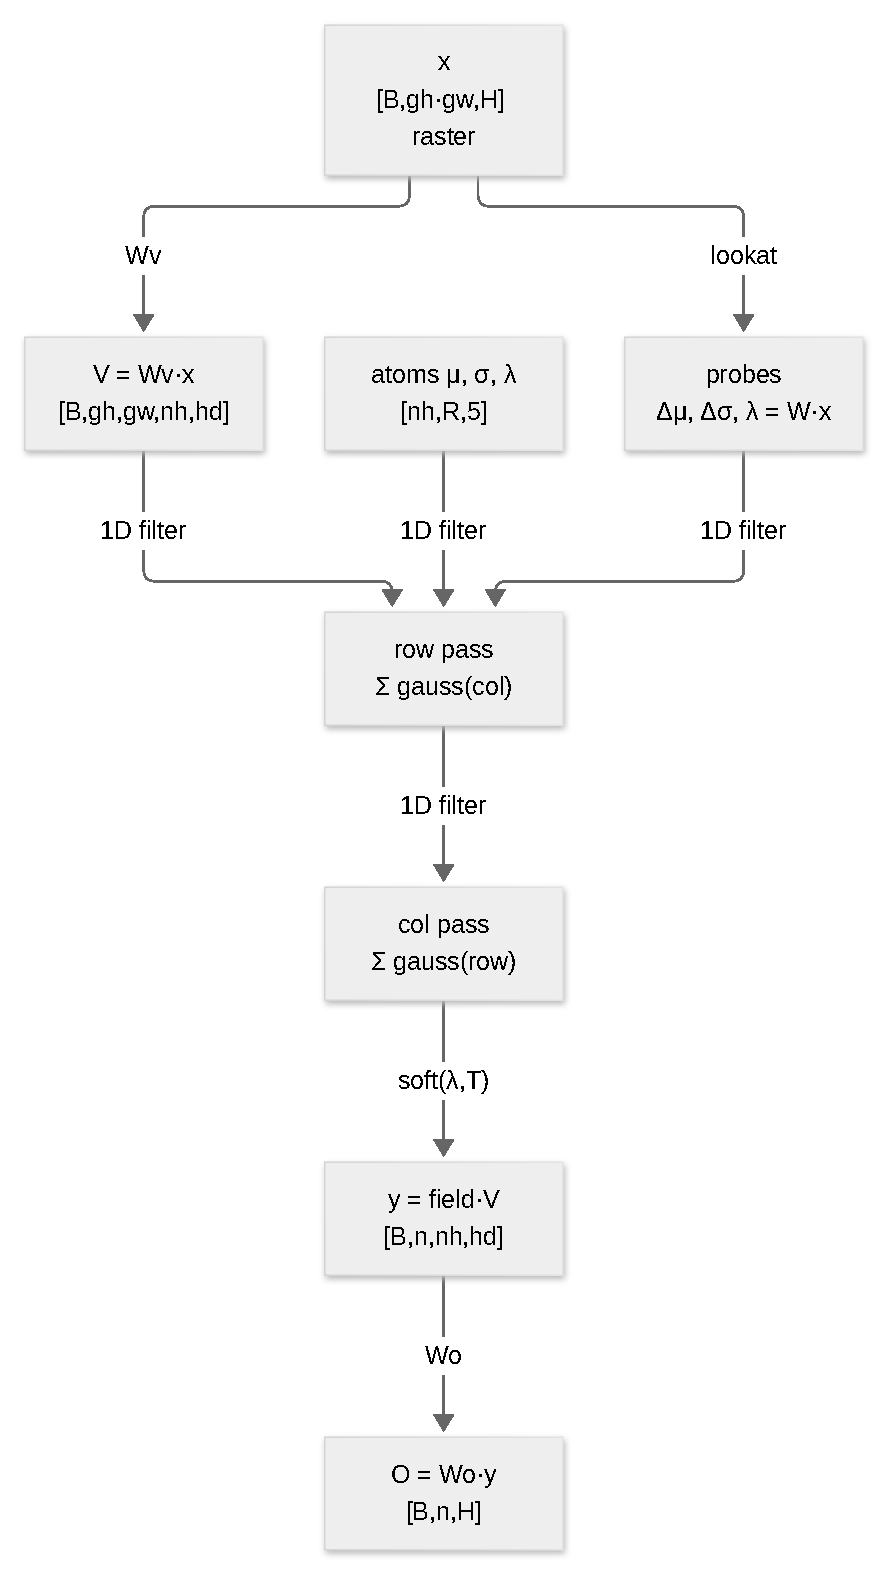
\includegraphics{../paper/figures/mixers/ssog.pdf}}
\caption{Flujo de datos de SSOG: los valores pasan por pasadas separables de filtrado gaussiano por filas y columnas para cada átomo, con direccionamiento opcional de los parámetros del átomo por contenido.}
\label{fig:mixer-ssog}
\end{figure}
\subsection{Formulación Matemática}
Sea el raster row-major de una rejilla $G_h \times G_w$ los tokens. El peso de atención del token $p$ al token $q$ es el log-sum-exp con softmax y temperatura de los log-pesos de los átomos evaluados en su desplazamiento:
\[
A(p, q) = \operatorname{softmax}_q\!\left( \tfrac{1}{\tau}\, s(p, q) \right),
\qquad
s(p, q) = \operatorname{logsumexp}_r \big( \log \lambda_r + \log \mathcal{N}(p - q;\ \mu_r, \sigma_r) \big),
\]
donde $\tau$ es una temperatura aprendible y $\mathcal{N}(\cdot\,;\mu_r, \sigma_r)$ es una Gaussiana 2D con covarianza diagonal. Como la Gaussiana 2D se factoriza, el campo con softmax se aplica de forma separable: por eje, $a_y[i, j] = \operatorname{softmax}_j(\log \mathcal{N}(\Delta y_{ij}; \mu_y, \sigma_y) / \tau)$ y análogamente $a_x$, seguido de
\[
Y = \sum_{r=1}^{R} \lambda_r\, \big( a_x^{(r)} \big( a_y^{(r)}\, V \big) \big),
\qquad V = x W_V,
\]
es decir, tres contracciones einsum por capa. Con direccionamiento por contenido (\texttt{lookat}) habilitado, sondas lineales inicializadas en cero predicen residuos por token acotados sobre los parámetros del campo detrás de compuertas softplus de arranque en frío:
\[
\mu \leftarrow \mu_0 + s_\mu \cdot m \cdot \tanh(W_\mu x), \qquad
\sigma \leftarrow \sigma_0 \, e^{s_\sigma \tanh(W_\sigma x)}, \qquad
\lambda \leftarrow \operatorname{softmax}\big( \log \lambda_0 + s_\lambda \tanh(W_\lambda x) \big),
\]
con $m$ el desplazamiento máximo en celdas de rejilla y escalas de compuerta $s_\bullet = \operatorname{softplus}(\cdot)$ inicializadas en $-8$ ($\approx 3 \times 10^{-4}$), de modo que el modelo comienza como un campo geométrico congelado y aprende cuánto abrir cada toma de contenido. Los anchos se reparametrizan como $\sigma = \operatorname{softplus}(\omega) + \epsilon + \sigma_{\text{piso}}$ para mantenerse estrictamente positivos.

\subsection{Pseudocódigo Algorítmico}
\begin{algorithmic}[1]
\State \textbf{Entrada:} estado oculto $x \in \mathbb{R}^{B \times N \times d}$ como raster $G_h \times G_w$, átomos $\{\mu_r, \omega_r, \log \lambda_r\}_{r=1}^{R}$ por cabeza, temperatura $\tau$
\State $V \gets x W_V$ reorganizado a $(B, G_h, G_w, H, d_h)$ \Comment{sin proyecciones Q/K}
\State $\sigma_r \gets \operatorname{softplus}(\omega_r) + \epsilon + \sigma_{\text{piso}}$ \Comment{anchos positivos}
\If{direccionamiento (lookat)}
    \State $\mu, \sigma, \lambda \gets$ residuos por token acotados vía sondas init-cero y compuertas \Comment{el contenido dirige}
\EndIf
\State $a_y \gets \operatorname{softmax}\!\big(\log \mathcal{N}(\Delta y; \mu_y, \sigma_y) / \tau\big)$, \quad $a_x \gets$ análogamente \Comment{kernels 1D, uno por átomo}
\State $Y \gets \sum_r \lambda_r\, a_x^{(r)} \big( a_y^{(r)} V \big)$ \Comment{pasada filas, pasada columnas, mezcla $\lambda$: sin $N \times N$}
\State \textbf{Salida:} $\mathbf{Y} W_O$ reorganizado a $(B, N, d)$
\end{algorithmic}

\subsection{Características Clave}
\begin{itemize}[leftmargin=*]
    \item \textbf{Complejidad de entrenamiento}: $\mathcal{O}(R \cdot N \sqrt{N} \cdot d)$ para $R$ átomos fijos---casi lineal solo por geometría, no por aproximación de kernels.
    \item \textbf{Complejidad de inferencia}: mismo costo por pasada; solo encoder (el campo separable no tiene formulación causal), por lo que no hay semánticas de caché KV.
    \item \textbf{Entrenable}: los átomos $\{\mu, \omega, \log\lambda\}$, la temperatura y las sondas de direccionamiento son completamente diferenciables; las compuertas de arranque en frío se abren durante la optimización.
    \item \textbf{Fortalezas}: prior geométrico fuerte (+17 pts sobre SDPA en datos pequeños con receta igualada; supera a SDPA en ImageNet-1k con 3M y 12M parámetros con $\sim$20\% menos parámetros y $\sim$30\% menos FLOPs); interpretable por diseño (cada cabeza son unos pocos blobs graficables---las capas tempranas se vuelven convoluciones encubiertas, las intermedias detectores de franjas, las tardes se vuelven globales); el campo vive en coordenadas, lo que otorga transferencia de resolución zero-shot.
    \item \textbf{Limitaciones}: solo encoder; requiere un raster row-major fijo $G_h \times G_w$ (ViT necesita \texttt{cls\_token=false}; las secuencias necesitan una rejilla $1 \times L$ explícita); los kernels de direccionamiento por query añaden un término de memoria; los resultados en lenguaje no están probados---allí el puntaje por contenido probablemente es estructural.
\end{itemize}

\section{Atención de Peso Rápido para Aprendizaje Continuo}
\label{sec:annex-fast-weight}

Este anexo cubre la familia Falcon \citep{zhang_falcon_2026}, un marco de atención de peso rápido que trata la transición recurrente del estado de peso rápido como una \textbf{regla de aprendizaje continuo en línea} bajo semántica autoregresiva de \emph{lectura tras escritura} (read-after-write, RAW). La observación central del marco es de alineación temporal: para el objetivo de predicción de prefijo, el ejemplo local de memoria rápida revelado en el paso $t$ es el \textbf{par prefix-alineado} $(x_t, y_t) = (\phi(k_{t-1}),\, v_t)$ --- desplazado un paso respecto a la asociación de mismo paso $(\phi(k_t), v_t)$ usada por DeltaNet y la atención lineal estándar. La asociación de mismo paso sigue siendo causal, pero optimiza un objetivo interno diferente. El marco deriva \textbf{actualizaciones de primer orden normalizadas} para dos objetivos (regresión de error cuadrático y producto interno negativo) y tres estructuras de tamaño de paso (escalar, por columna, ventana deslizante), dando seis variantes: Falcon-1/2/3 (familia de regresión) y Falcon-1A/2A/3A (familia de producto interno). Las seis variantes están implementadas en el código bajo \texttt{model.attention.falcon} con un bloque de configuración compartido, cada una proporcionando tanto un escaneo recurrente de referencia como un kernel chunk-parallel estilo SSD.

\subsection{Preliminares: Alineación, Normalización, Renormalización}

\paragraph{Semántica de lectura tras escritura.} Con mapas de características $\phi(k_t)$ (QK-RMSNorm por defecto), el flujo prefix-alineado fija $x_t = \phi(k_{t-1})$ para $t \ge 2$ con centinela de frontera $x_1 = 0$; la lectura es $o_t = S_t^\top \phi(q_t)$. La escritura en el paso $t$ por tanto actualiza la memoria \emph{antes} de que la consulta del paso $t+1$ la lea, de modo que ninguna clave se asocia jamás con su propio token.

\paragraph{Tamaños de paso normalizados.} Un paso de gradiente sobre el objetivo local $\ell_t(S)$ con el denominador acoplado al objetivo da
\[
\eta_t = \frac{\beta_t}{\text{estadístico}_t + \lambda_t + \varepsilon}, \qquad \beta_t \in (0, 2),
\]
donde el estadístico es la energía cuadrática de la clave $\|x_t\|^2$ (Falcon-1/1A/2/2A), el estadístico espectral de ventana $\mu_t^{(B)} = \lambda_{\max}(X^\top X)/B_t$ (Falcon-3), o la energía media de ventana $\bar{E}_t^{(B)}$ (Falcon-3A). La normalización acoplada al objetivo garantiza descenso por paso y elimina la sensibilidad a la escala de las tasas de aprendizaje fijas. La ganancia de \textbf{plasticidad} $\beta_t$, el ridge de \textbf{olvido} $\lambda_t$, la \textbf{alineación} temporal y la ventana de repetición $B$ quedan así separados como cuatro perillas previamente entrelazadas.

\paragraph{Renormalización de decaimiento positivo.} Cuando $\lambda_t > 0$, la contracción por paso $\alpha_t = \min(\eta_t \lambda_t,\, 1 - \varepsilon_\gamma)$ debe aplicarse de forma estable. La implementación fija $\alpha_t$ estrictamente por debajo de $1$, calcula prefijos logarítmicos chunk-locales en fp32 vía $\log(1 - \alpha_t)$ y sumas acumuladas, reescala los generadores al dominio sin decaimiento ($\tilde{\eta}_t = \eta_t / \gamma_t$, $\tilde{v}_t = v_t / c_{t-1}$ con $c_{t-1} = \prod_{r \le t-1} \gamma_r$) y reescala salidas y el estado emitido por el $\delta$ acumulado. Los centinelas de frontera son $(\alpha_1, \gamma_1) = (0, 1)$ y $\eta_1 = 0$, de modo que el primer paso es una lectura pura.

\subsection{La Familia de Regresión (Falcon-1/2/3)}

El objetivo de error cuadrático sobre el par desplazado es
\[
\ell_t(S) = \tfrac{1}{2}\|v_t - S^\top x_t\|^2 + \tfrac{\lambda_t}{2}\|S\|_F^2,
\qquad
\nabla_S \ell_t = x_t (S^\top x_t - v_t)^\top + \lambda_t S,
\]
que es $L_t$-suave con $L_t = \|x_t\|^2 + \lambda_t$.

\subsubsection{Falcon-1: Regresión NLMS Escalar}

\begin{figure}[H]
\centering
\fitfigure{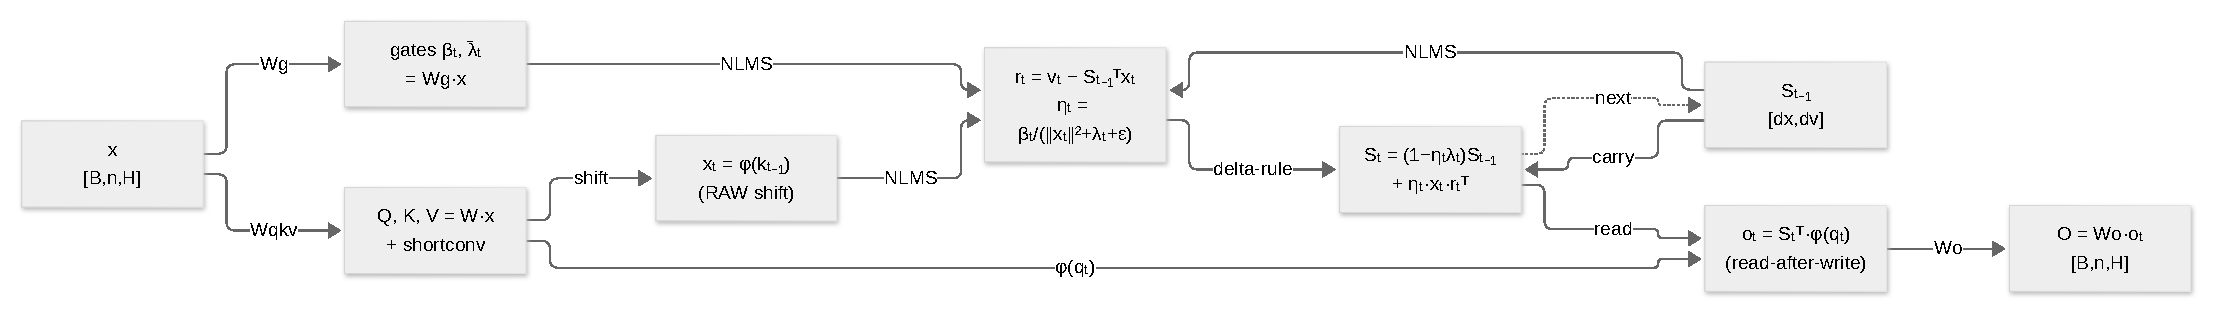
\includegraphics{../paper/figures/mixers/falcon1.pdf}}
\caption{Flujo de datos de Falcon-1: el par clave/valor alineado al prefijo impulsa una actualización escalar NLMS por regla delta del estado de pesos rápidos.}
\label{fig:mixer-falcon1}
\end{figure}

La variante escalar de la regla delta --- la recursión NLMS clásica del filtrado adaptativo, mejorada con el flujo desplazado y un ridge explícito:
\[
S_t = (1 - \eta_t \lambda_t)\, S_{t-1} + \eta_t\, x_t \big(v_t - S_{t-1}^\top x_t\big)^\top,
\qquad
o_t = S_t^\top \phi(q_t).
\]
Con $\varepsilon = 0$, $\lambda_t = 0$ y la asignación sin desplazar $x_t = \phi(k_t)$ esto recupera DeltaNet exactamente. La eigenestructura de la transición $A_t = \gamma_t I - \eta_t x_t x_t^\top$ (con $\gamma_t = 1 - \eta_t\lambda_t$) muestra que la dirección de escritura se contrae por $1 - \beta_t$ mientras el subespacio ortogonal lleva $\gamma_t$: $\beta_t > 1$ produce un cambio de signo estable a lo largo de la dirección de escritura, útil para seguimiento de estado. La forma chunk-parallel usa la representación WY $\prod_s (I - \eta_s x_s x_s^\top) = I - U T U^\top$ con una única solución triangular unitaria inferior de residuo simple $L = \operatorname{tril}(G, -1) + I$ donde $G = X^\top X$ (Algoritmo~8 del artículo), tras la renormalización de decaimiento positivo.

\subsubsection{Falcon-2: Regresión NLMS por Columnas}

\begin{figure}[H]
\centering
\fitfigure{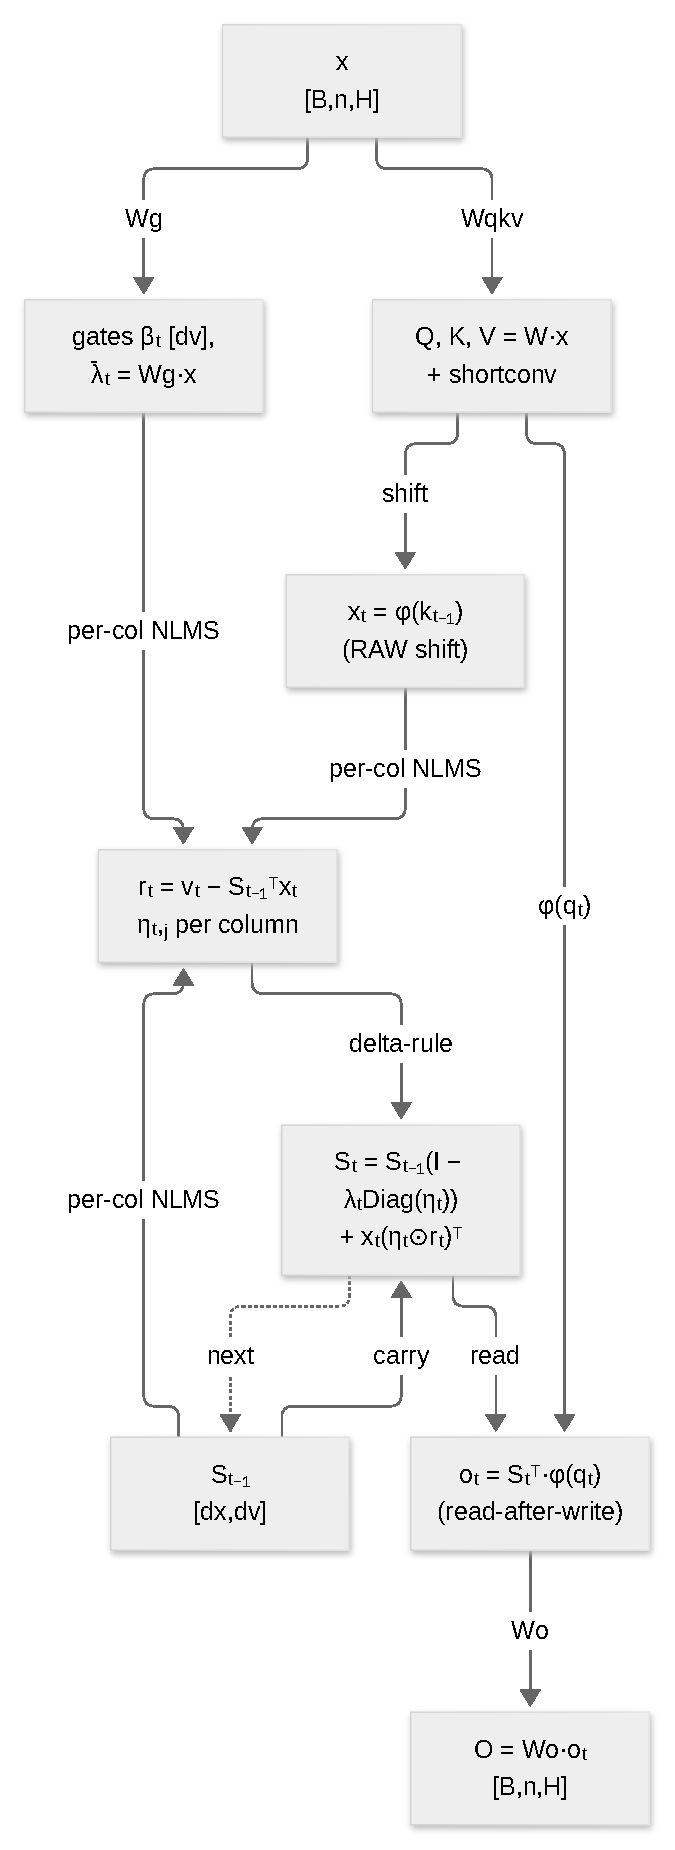
\includegraphics{../paper/figures/mixers/falcon2.pdf}}
\caption{Flujo de datos de Falcon-2: tamaños de paso NLMS por columna actualizan el estado de pesos rápidos canal a canal.}
\label{fig:mixer-falcon2}
\end{figure}

La pérdida ridge se descompone a lo largo de las coordenadas de valor, de modo que cada canal de valor $j$ recibe su propio tamaño de paso compartiendo el normalizador NLMS:
\[
\eta_{j,t} = \frac{\beta_{j,t}}{\|x_t\|^2 + \lambda_t + \varepsilon},
\qquad
S_t = S_{t-1}\big(I - \lambda_t \operatorname{Diag}(\boldsymbol{\eta}_t)\big) + x_t \big(\boldsymbol{\eta}_t \odot \mathbf{r}_t\big)^\top .
\]
El kernel chunk-parallel forma el Gram de claves compartido $G = X^\top X$ y resuelve el lote de sistemas triangulares unitarios inferiores por canal $L_j = I + \operatorname{tril}\big(G \odot (\Sigma_j \Sigma_j^\top), -1\big)$ con $\Sigma = \sqrt{\tilde{\boldsymbol{\eta}}}$ (Algoritmo~1). Definida pero no evaluada por separado en el artículo.

\subsubsection{Falcon-3: Regresión de Minilote con Ventana Deslizante}

\begin{figure}[H]
\centering
\fitfigure{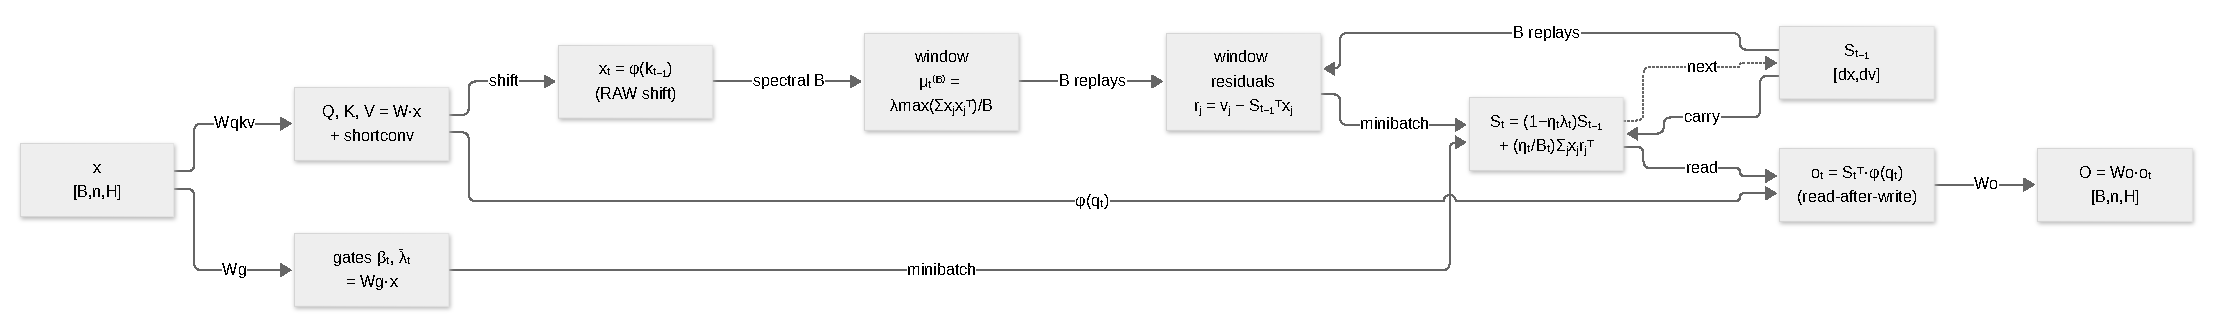
\includegraphics{../paper/figures/mixers/falcon3.pdf}}
\caption{Flujo de datos de Falcon-3: una ventana deslizante de pares alineados al prefijo aporta el estadístico espectral y la escritura por minilote.}
\label{fig:mixer-falcon3}
\end{figure}

Repetición acotada (bounded rehearsal): cada paso regresa la memoria rápida sobre los últimos $B_t \le B$ pares prefix-alineados, con \emph{todos los residuos de ventana evaluados en el estado pre-actualización} $S_{t-1}$:
\[
\mu_t = \frac{\lambda_{\max}\big(X_{\mathcal{I}_t}^\top X_{\mathcal{I}_t}\big)}{B_t},
\qquad
\eta_t = \frac{\beta_t}{\mu_t + \lambda_t + \varepsilon},
\qquad
S_t = (1 - \eta_t \lambda_t)\, S_{t-1} + \frac{\eta_t}{B_t} \sum_{j \in \mathcal{I}_t} x_j \big(v_j - S_{t-1}^\top x_j\big)^\top ,
\]
con $\mathcal{I}_t = \{\max(2, t - B + 1), \dots, t\}$. El promediado por ventana mantiene la magnitud de la actualización invariante a $B$: cada par se repite en exactamente $B$ actualizaciones consecutivas con peso $1/B$, por lo que su inyección acumulada es independiente de $B$. El estado por sí solo \emph{no} es Markov: la continuación exacta requiere una cola FIFO de los últimos $B - 1$ pares, y los kernels chunk recogen una porción extendida con $|\mathcal{J}| \le C + B - 1$. La forma chunk-parallel es una recurrencia afín de rango $B$ resuelta por sustitución hacia adelante por bloques sobre el espacio de índices extendido (tiempo $\times$ rango), con componentes de rango del mismo tiempo desacoplados (Algoritmo~3).

\subsection{La Familia de Producto Interno (Falcon-1A/2A/3A)}

El objetivo de producto interno negativo
\[
\ell_t^{\mathrm{ip}}(S) = -\langle S^\top x_t,\, v_t \rangle + \tfrac{\lambda_t}{2}\|S\|_F^2
\qquad \Rightarrow \qquad
\nabla_S \ell_t^{\mathrm{ip}} = -x_t v_t^\top + \lambda_t S
\]
produce escrituras puramente aditivas (hebbianas) con ganancias normalizadas por energía.

\subsubsection{Falcon-1A y Falcon-2A}

\begin{figure}[H]
\centering
\fitfigure{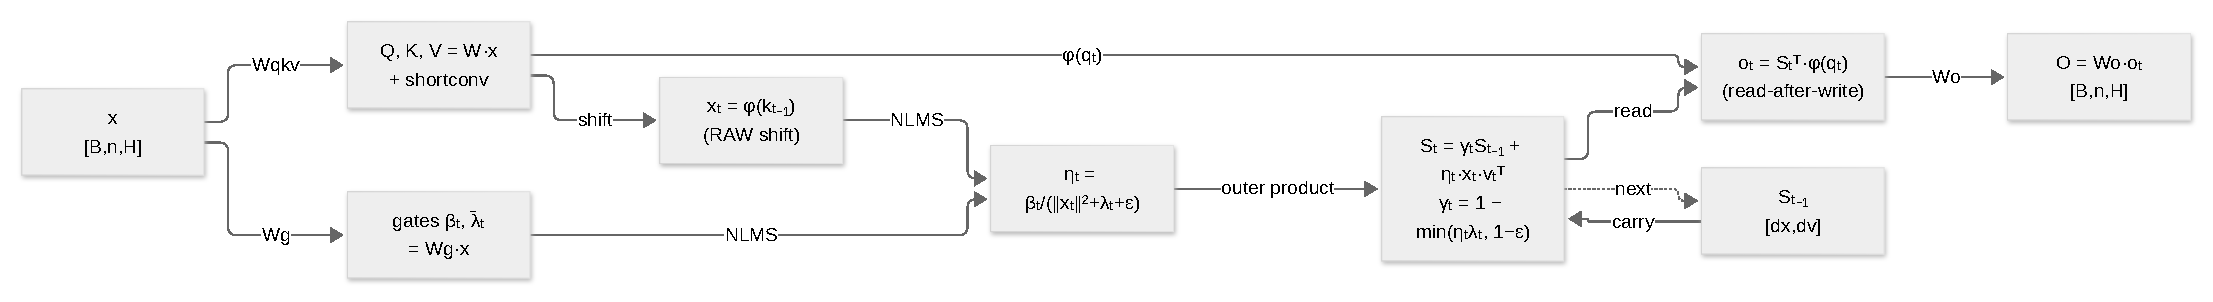
\includegraphics{../paper/figures/mixers/falcon1a.pdf}}
\caption{Flujo de datos de Falcon-1A: una escritura aditiva (hebbiana) normalizada por energía con decaimiento derivado.}
\label{fig:mixer-falcon1a}
\end{figure}

\begin{figure}[H]
\centering
\fitfigure{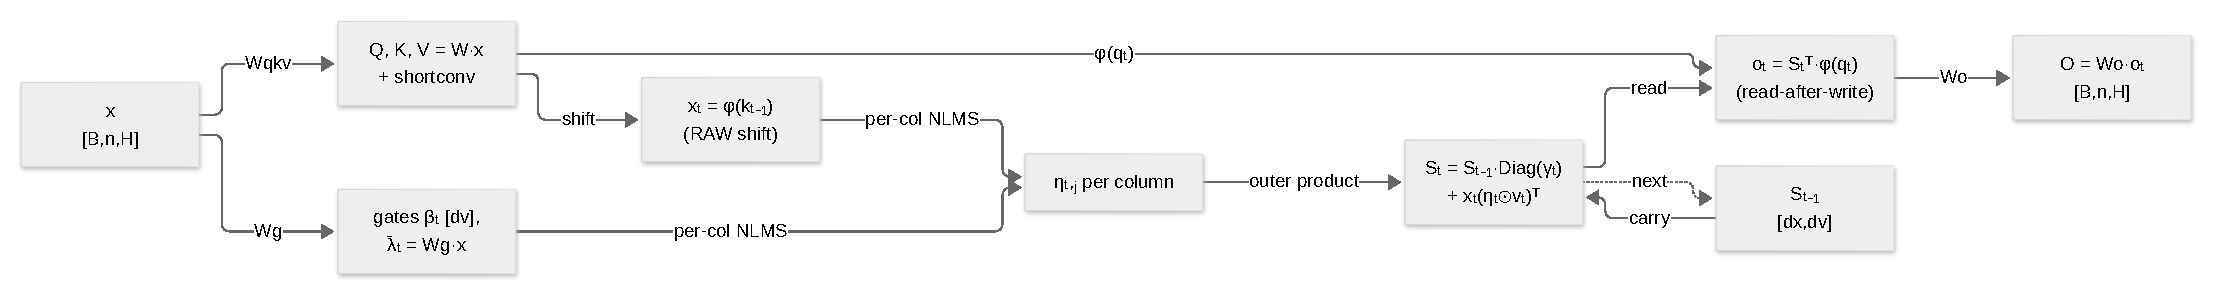
\includegraphics{../paper/figures/mixers/falcon2a.pdf}}
\caption{Flujo de datos de Falcon-2A: escrituras aditivas por columna con decaimiento por canal.}
\label{fig:mixer-falcon2a}
\end{figure}

\[
\text{Falcon-1A:}\quad S_t = \gamma_t S_{t-1} + \eta_t\, x_t v_t^\top,
\quad \gamma_t = 1 - \min(\eta_t \lambda_t,\, 1 - \varepsilon_\gamma);
\qquad
\text{Falcon-2A:}\quad S_t = S_{t-1}\operatorname{Diag}(\boldsymbol{\gamma}_t) + x_t (\boldsymbol{\eta}_t \odot v_t)^\top .
\]
Con $\lambda_t = 0$ y la asignación sin desplazar esto es exactamente la atención lineal estándar / acumulación Mamba-2; el flujo desplazado lo convierte en la variante next-latent desplazada un paso. El denominador de la familia A no lo exige la curvatura (el objetivo es lineal) --- conserva la escritura normalizada por energía como estabilizador de magnitud. La forma chunk-parallel es atención lineal con máscara de decaimiento $M_{t,i} = \eta_i \prod_{r=i+1}^{t} \gamma_r$ (máscaras por canal para Falcon-2A).

\subsubsection{Falcon-3A: Producto Interno con Ventana Deslizante}

\begin{figure}[H]
\centering
\fitfigure{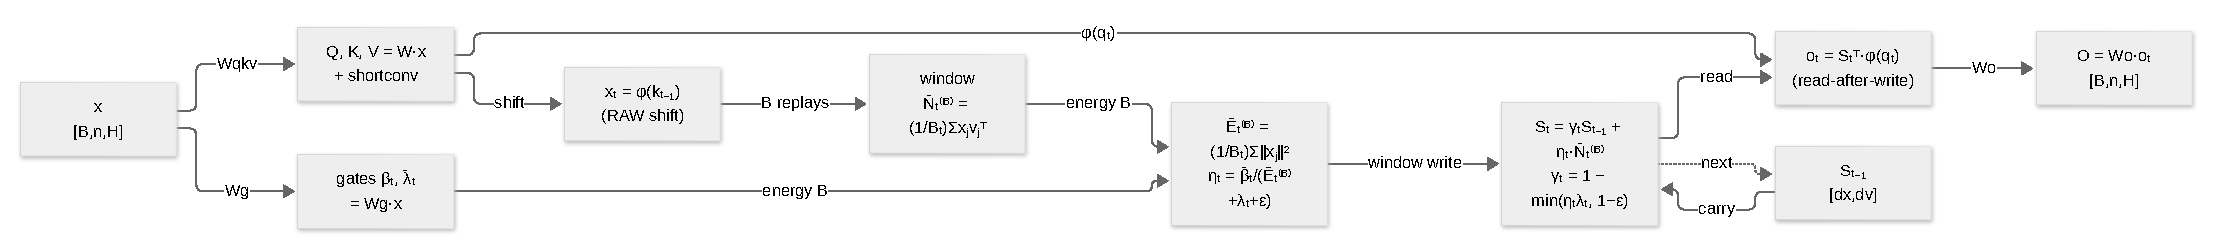
\includegraphics{../paper/figures/mixers/falcon3a.pdf}}
\caption{Flujo de datos de Falcon-3A: un estadístico de energía media en ventana deslizante normaliza la escritura aditiva de la ventana.}
\label{fig:mixer-falcon3a}
\end{figure}

La variante aditiva con ventana --- la mejor configuración de extrapolación de longitud de la familia:
\[
\bar{N}_t^{(B)} = \frac{1}{B_t} \sum_{j \in \mathcal{I}_t} x_j v_j^\top,
\qquad
\bar{E}_t^{(B)} = \frac{1}{B_t} \sum_{j \in \mathcal{I}_t} \|x_j\|^2,
\qquad
\eta_t = \frac{\beta_t}{\bar{E}_t^{(B)} + \lambda_t + \varepsilon},
\qquad
S_t = \gamma_t S_{t-1} + \eta_t\, \bar{N}_t^{(B)} .
\]
La máscara de decaimiento con banda de ventana factoriza como $M = D \cdot \operatorname{Diag}(\boldsymbol{\eta}) \cdot A$, donde $A$ es el operador de ventana de banda $B$ y $D$ el kernel de decaimiento causal, evaluada sobre la porción extendida (Algoritmo~4).

\subsection{Interfaz de Configuración}

Las seis variantes comparten un bloque anidado, \texttt{model.attention.falcon}, seleccionado mediante las entradas de \texttt{layer\_pattern} \texttt{falcon1\_attn}, \texttt{falcon2\_attn}, \texttt{falcon3\_attn}, \texttt{falcon1a\_attn}, \texttt{falcon2a\_attn}, \texttt{falcon3a\_attn}:

\begin{table}[H]
\centering
\small
\begin{tabularx}{0.95\linewidth}{llX}
\toprule
\textbf{Clave} & \textbf{Por defecto} & \textbf{Descripción} \\
\midrule
\texttt{chunk\_size} & $64$ & Tamaño de chunk de los kernels chunk-parallel; \texttt{null} selecciona el escaneo recurrente de referencia \\
\texttt{qk\_norm} & \texttt{rms\_norm} & Normalización QK (\texttt{rms\_norm} o \texttt{l2\_norm}); RMSNorm calculado en fp32 \\
\texttt{beta\_mode} & \texttt{ctx\_eta} & Parametrización de la compuerta de plasticidad: \texttt{static}, \texttt{ctx\_beta} (ganancia condicionada al contenido) o \texttt{ctx\_eta} (paso normalizado condicionado al contenido) \\
\texttt{lambda\_mode} & \texttt{ctx} & Compuerta de olvido: \texttt{static} o \texttt{ctx} (acoplada en escala con el estadístico de curvatura desacoplado) \\
\texttt{beta} / \texttt{lambda} & $1.0$ / $0.0$ & Ganancia y ridge estáticas (usadas cuando el modo correspondiente es \texttt{static}) \\
\texttt{window} & $4$ & Ventana deslizante $B$ (solo Falcon-3 / Falcon-3A) \\
\texttt{short\_conv} / \texttt{conv\_kernel} & \texttt{true} / $4$ & Convoluciones cortas causales en profundidad sobre las proyecciones q/k/v \\
\texttt{eps} / \texttt{eps\_gamma} & $10^{-6}$ / $10^{-4}$ & Estabilizador del tamaño de paso y piso de fijación del decaimiento positivo \\
\bottomrule
\end{tabularx}
\caption{Perillas de configuración compartidas de Falcon (\texttt{model.attention.falcon}). Cada variante expone además un opt-out de codificación posicional por mezclador \texttt{falcon\{1,2,3,1a,2a,3a\}\_attn\_use\_pe}, por defecto \texttt{False} como los demás mezcladores recurrentes/de decaimiento.}
\label{tab:falcon-knobs}
\end{table}

Notas de implementación: los kernels recurrente y chunk-parallel están verificados numéricamente equivalentes (chunk $\equiv$ recurrente a $\le 3.6 \times 10^{-7}$ en las seis variantes, incluidas las rutas con decaimiento, multi-chunk y ventana); los gradientes fluyen a través de las islas de solución triangular en fp32 (los generadores de características toman solo $\sqrt{\tilde{\eta}}$ mientras los objetivos de valor toman $\sqrt{\tilde{\eta}}\, e^{-u_{t-1}}$, con la raíz cuadrada fijada en $10^{-12}$ para retropropagación sin NaN en la frontera $\eta = 0$); los exponentes positivos se fijan en $80$.

\subsection{Resultados Publicados}

\begin{table}[H]
\centering
\small
\begin{tabularx}{0.95\linewidth}{Xcccc}
\toprule
\textbf{Modelo (124M, 49.2B tokens FineWeb-Edu)} & \textbf{WikiText ppl} & \textbf{LMB. ppl} & \textbf{FineEdu ppl} & \textbf{Prom. 0-shot} \\
\midrule
Transformer (RoPE) & 33.25 & 47.43 & 17.38 & 48.16 \\
Mamba-2 & 34.53 & 48.74 & 17.70 & 48.80 \\
DeltaNet & 34.19 & 52.84 & 17.84 & 48.88 \\
Gated DeltaNet & 30.99 & 46.70 & 17.32 & 48.78 \\
Falcon-1A.3 & 34.02 & 49.84 & 17.40 & 48.95 \\
Falcon-1.3 & 33.00 & 48.70 & \textbf{17.10} & \textbf{49.18} \\
\bottomrule
\end{tabularx}
\caption{Resultados de modelado de lenguaje reportados por \citet{zhang_falcon_2026} a 124M de parámetros. En extrapolación de longitud para sumas de dígitos variables (33--48 dígitos), Falcon-3A.3 alcanza \textbf{87.2\%} de precisión media frente a 65.8\% de un Transformer con RoPE y 85.9\% de Falcon-1A.3: la familia de producto interno lleva la aritmética, mientras que la familia de regresión lleva la perplejidad.}
\label{tab:falcon-results}
\end{table}

\subsection{Relación con Trabajos Previos}

\begin{itemize}[leftmargin=*]
    \item \textbf{DeltaNet}: la regla delta es el paso de descenso de gradiente del objetivo de error cuadrático con el emparejamiento de mismo paso; Falcon lo recupera con el cambio crítico de índice más normalización acoplada al objetivo y contracción $\lambda_t$ explícita.
    \item \textbf{Gated DeltaNet}: añade una compuerta de arrastre aprendida libre; Falcon \emph{deriva} el arrastre $\gamma_t = 1 - \eta_t \lambda_t$ del objetivo local y la parametrización de paso normalizada en lugar de añadir una compuerta independiente, y usa por defecto QK-RMSNorm en lugar de normalización $\ell_2$.
    \item \textbf{Atención lineal / Mamba-2}: el numerador aditivo es un paso de gradiente del objetivo de producto interno con la asignación sin desplazar; los kernels chunkwise reutilizan el esquema SSD.
    \item \textbf{TTT / Titans / ATLAS}: actualizaciones de peso rápido como entrenamiento en tiempo de prueba; Falcon-3 es una especialización de ventana deslizante de la vista de objetivo interno con alineación estricta next-latent.
    \item \textbf{Filtrado adaptativo (LMS/NLMS/RLS)}: Falcon importa los principios de estabilidad y normalización de NLMS a la atención de peso rápido bajo causalidad estricta.
\end{itemize}

\subsubsection{Cuándo Usar Cada Variante}

\begin{enumerate}[leftmargin=*]
    \item \textbf{Falcon-1}: la mejor perplejidad de modelado de lenguaje de la familia (FineEdu 17.10, superando a Gated DeltaNet 17.32); olvido principista ligado al objetivo local.
    \item \textbf{Falcon-2}: plasticidad más fina que Falcon-1 al costo de kernels chunk por canal más pesados; sin evaluación en el artículo.
    \item \textbf{Falcon-3}: horizonte de repetición controlado con estadísticos de ventana exactos; el kernel más complejo.
    \item \textbf{Falcon-1A}: variante aditiva simple y estable; segunda mejor extrapolación de longitud (85.9\%).
    \item \textbf{Falcon-2A}: granularidad de olvido por canal; sin evaluación.
    \item \textbf{Falcon-3A}: la mejor extrapolación de longitud del artículo (87.2\% en sumas de 33--48 dígitos); carry de tareas aritméticas.
\end{enumerate}
\section{Caché KV y Decodificación Incremental}
\label{sec:annex-kv-cache}

La decodificación autorregresiva está dominada por una asimetría estructural: la etapa de \emph{prefill} procesa el prompt completo en una sola pasada cuadrática, mientras que cada paso de decodificación añade un único token y sólo necesita una fila de consulta nueva contra una historia ya calculada. Recomputar la secuencia completa en cada paso convierte la generación en un procedimiento de $\mathcal{O}(S^2)$ por token; mantener la historia por capa la convierte en $\mathcal{O}(S)$ por token con trabajo de tamaño constante por posición nueva. Este anexo documenta el subsistema de caché KV del toolkit (\texttt{src/model/cache/}), los contratos de corrección que hacen numéricamente intercambiables la ejecución con y sin caché, las recetas incrementales por familia, y los cuantizadores de escritura y las políticas de expulsión de lectura que se apilan sobre él.

Tres compromisos de diseño enmarcan todo lo anterior. Primero, la caché es \emph{opcional}: sin \texttt{inference.kv\_cache.enabled} (por defecto), la generación ejecuta el bucle original de recomputación completa de forma bit-idéntica. Segundo, la caché es \emph{central y declarativa}: un único gestor se propaga por el modelo, y un registro de capacidades por mezclador decide qué capas pueden cachear --- nunca al revés. Tercero, la caché \emph{nunca es fatal} (decisión D5): una capa cuya formulación de origen no admite una forma incremental exacta se ejecuta sin caché en silencio, de modo que habilitarla sólo puede cambiar la velocidad, no la corrección ni la disponibilidad.

\subsection{Motivación y Alcance}

Sea $S$ la longitud del prompt y $T$ el número de tokens generados. Sin caché, el paso $t$ introduce $S+t-1$ tokens por todas las capas y descarta todas las claves y valores intermedios, con un trabajo de atención total
\[
\mathcal{O}\!\left(\sum_{t=0}^{T-1} (S+t)^2\right) \;=\; \mathcal{O}\!\left(T S^2 + T^2 S + T^3\right).
\]
Con caché, el prefill cuesta $\mathcal{O}(S^2)$ una vez y cada paso de decodificación cuesta $\mathcal{O}(S+t)$:
\[
\mathcal{O}\!\left(S^2 + \sum_{t=0}^{T-1}(S+t)\right) \;=\; \mathcal{O}\!\left(S^2 + TS + T^2\right).
\]
La diferencia es la conocida entre re-codificar una conversación y continuarla.

El subsistema cubre los cuarenta y cuatro tipos de capa despachables. Veintiséis tienen ramas incrementales verificadas por paridad; el resto queda registrado con una justificación explícita, basada en el artículo, para ejecutarse sin caché (\S\ref{sec:kv-fallbacks}). La cuantización y la expulsión son ortogonales a la matemática del mezclador: los códecs transforman tensores en \emph{escritura} y las políticas actúan en \emph{lectura}, de modo que el mismo códec \texttt{int8} o \texttt{int4\_kivi} sirve a un slot denso, latente o de anillo sin código por mezclador \citep{kivi_liu_2024,kvquant_hooper_2024,skvq_duanmu_2024}.

\subsection{Arquitectura de la Caché}
\label{sec:kv-architecture}

\subsubsection{Gestor Central e Identidad de Capa}

La unidad de cacheo es una capa lógica, no un módulo. El encoder puede re-ejecutar la misma pila física \texttt{num\_loops} veces (profundidad en bucle) y, bajo Hyperloop, dividirla en un bloque inicial, un bloque medio en bucle y un bloque final. El mismo objeto \texttt{HybridLayer} desempeña por tanto varios roles distintos durante una pasada. La caché indexa cada slot por el \textbf{índice de capa lógica} global
\[
\ell \;=\; 0,\dots,\, \texttt{num\_layers}\times\texttt{num\_loops}-1 ,
\]
que el encoder ya propaga a cada llamada de mezclador. Dos roles lógicos nunca comparten almacenamiento aunque compartan pesos.

\begin{algorithm}[H]
\caption{Bucle de generación con caché (prefill + decodificación)}
\begin{algorithmic}[1]
\Require ids del prompt $\mathbf{x}_{1:S}$; configuración de generación $\theta$; modelo $f$
\Ensure ids generados
\State $\mathcal{C} \gets \textsc{Cache.new}(f,\theta)$ \Comment{slots perezosos, cola de tokens, cursor de escritura}
\State $\mathbf{L}, \mathcal{C} \gets f(\mathbf{x}_{1:S}; \text{past}=\mathcal{C}, \text{use\_cache}=\top, \text{return\_cache}=\top)$ \Comment{prefill}
\State $\mathbf{z} \gets \mathbf{L}_{:,S,:}$
\For{$t \gets 0$ \textbf{hasta} $T-1$}
    \State $y \gets \textsc{Sample}(\mathbf{z};\theta)$ \Comment{greedy, top-$k$, top-$p$}
    \State \textbf{añadir} $y$ a la salida
    \If{$t < T-1$}
        \State $p \gets \mathcal{C}.\text{next\_position}()$
        \State $\mathbf{L}, \mathcal{C} \gets f(y; \text{past}=\mathcal{C}, \text{use\_cache}=\top, \text{cache\_position}=p, \text{return\_cache}=\top)$
        \State $\mathbf{z} \gets \mathbf{L}_{:,-1,:}$
    \EndIf
\EndFor
\end{algorithmic}
\end{algorithm}

El gestor posee el diccionario de slots por capa, una cola FIFO de ids de tokens recientes (consumida por mezcladores de nivel de token como Engram), un cursor de escritura que avanza en cada pasada, y el códec de cuantización y la política de expulsión resueltos. La creación de slots es perezosa y la dispara la capa en su primer uso, de modo que un \texttt{layer\_pattern} heterogéneo --- por ejemplo una capa densa, una latente y una recurrente en una misma pila --- mantiene tres tipos de slot distintos sin casos especiales. La reversión es una operación de primera clase: \texttt{truncate(n)} conserva las primeras $n$ posiciones en todos los slots (truncado de listas barato con contabilidad de longitud; los slots de estado recurrente son no-ops porque no están indexados por posición), que es la primitiva que requieren la decodificación especulativa y la verificación de salida temprana \citep{layerskip_elhoushi_2024}.

\subsubsection{Slots Tipados}

Seis tipos de slot cubren la taxonomía de \S\ref{sec:kv-recipes}. Los slots indexados por posición almacenan una lista ordenada de \emph{partes}; una parte es de precisión completa o una carga codificada, y la lectura concatena $\big[\text{sinks} \mid \text{historia} \mid \text{ventana protegida}\big]$.

\begin{table}[H]
\centering
\small
\begin{tabularx}{0.98\linewidth}{l L{0.34\linewidth} X}
\toprule
\textbf{Tipo de slot} & \textbf{Almacena} & \textbf{Usado por} \\
\midrule
\texttt{kv} & claves y valores post-RoPE $(\text{B},H_{kv},T,d)$; posiciones absolutas; extras por token opcionales & mezcladores softmax cuadráticos \\
\texttt{latent\_kv} & flujos de bajo rango con nombre: latente $\mathbf{c}_{KV}$, clave RoPE desacoplada, claves agrupadas, valores latentes & familia latente \\
\texttt{state} & una matriz recurrente (+ acumuladores de compuerta), actualizada in situ; memoria constante & familia recurrente / lineal \\
\texttt{ring} & K/V acotados por capacidad con una región de sinks fijada & familia de ventana deslizante \\
\texttt{conv\_tail} & últimas $k-1$ filas pre-convolución (FIFO) & convoluciones causales cortas \\
\texttt{token\_tail} & últimos $n$ ids de token & búsqueda de n-gramas de Engram \\
\bottomrule
\end{tabularx}
\caption{Slots de caché tipados. Los tipos indexados por posición (\texttt{kv}, \texttt{ring}, \texttt{latent\_kv}) llevan metadatos de posición absoluta, de modo que los huecos por expulsión mantienen distancias relativas correctas; \texttt{state} y \texttt{conv\_tail} no tienen posición y nunca se expulsan.}
\label{tab:kv-slots}
\end{table}

\subsubsection{Registro de Capacidades}

Un registro congelado por cada valor del enum \texttt{layer\_pattern} declara si una capa cachea y cómo:
\[
\textsc{CacheSpec} \;=\; \big(\texttt{supported},\ \texttt{slot\_type},\ \texttt{slot\_types},\ \texttt{extras},\ \texttt{notes}\big).
\]
El registro es la fuente única de verdad consultada tanto en ejecución (resolución de slot) como estáticamente (avisos de configuración). Una capa recibe un slot sólo cuando la formulación de su mezclador admite caché \emph{y} existe una rama incremental implementada y verificada por paridad; en caso contrario recibe \texttt{None} y ejecuta la ruta legada. El registro es, por tanto, también el inventario honesto del proyecto sobre qué significa cachear para cada artículo: \texttt{supported} registra la formulación de origen, el conjunto implementado registra el estado de ingeniería, y \texttt{notes} registra el motivo.

\subsubsection{Propagación en el Forward y Semántica de Respaldo}

Todos los cambios de firma son aditivos y por defecto reproducen el comportamiento legado:
\begin{align*}
f_{\text{mixer}}&(\mathbf{x}; \ell, \text{pe}, \texttt{cache}=\varnothing, \texttt{cache\_position}=\varnothing),\\
f_{\text{model}}&(\mathbf{x}; \texttt{past\_key\_values}=\varnothing, \texttt{use\_cache}=\bot, \texttt{return\_cache}=\bot).
\end{align*}
\texttt{HybridLayer} resuelve el slot una vez por llamada y respeta las cuatro formas históricas de despacho: el lineal sin estado (\texttt{mamba}) se invoca sin argumentos porque no tiene nada que cachear; los dos mezcladores que reemplazan el flujo completo (\texttt{ode}, \texttt{retnet}) reciben el slot sólo cuando su especificación lo admite; Engram recibe además \texttt{input\_ids}; el resto de mezcladores recibe \texttt{cache} y \texttt{cache\_position}. Las capas no admitidas o deshabilitadas se invocan exactamente como antes, lo que mantiene bit-idéntica la ruta sin caché.

\subsection{Contratos de Corrección}
\label{sec:kv-correctness}

La ejecución con y sin caché debe coincidir en la fila de consulta que comparten: la última fila de una pasada completa y la fila producida por un paso de decodificación. Los contratos siguientes establecen esa coincidencia.

\subsubsection{Almacenamiento Post-RoPE y el Calendario Absoluto}

Las claves se almacenan \emph{después} de la transformación rotatoria, la convención de la industria: la caché guarda los vectores ya rotados y no hace falta re-rotar cuando un anillo da la vuelta. El requisito es que la rotación use posiciones absolutas a ambos lados de la frontera de la caché. RoPE, HoPE y sinusoidal-rotatoria aceptan un desplazamiento de posición $\pi_0$ y sitúan los tokens entrantes en
\[
\pi_i = \big(\pi_0 + i\big)\cdot \texttt{scaling}, \qquad i = 0,\dots,S_{\text{nuevo}}-1 ,
\]
de modo que un paso de decodificación en el cursor $p$ rota exactamente como lo hizo la pasada completa en la posición $p$. Los metadatos del slot versionan el factor de escalado; un cambio en tiempo de ejecución del calendario RoPE invalida las claves ya rotadas y se reporta como error de configuración al inicio de la generación, nunca a mitad de decodificación \citep{su_rope_2024,dai_hope_2025}.

\subsubsection{Sesgos Aditivos en las Puntuaciones}

ALiBi y BAM inyectan la posición a través de la matriz de puntuaciones, así que no llevan tensor posicional en la caché --- precisamente su atractivo para la extrapolación de longitud \citep{press_alibi_2022,bianchessi_bam_2025}. El constructor de matriz completa se generaliza a uno de ventana sobre posiciones absolutas de consulta y clave:
\[
b_{h,i,j} \;=\; -\,\text{pendiente}_h \cdot \big|q_i - \kappa_j\big| \quad\text{(ALiBi)},
\qquad
b_{h,i,j} \;=\; -\Big(\big|\kappa_j - \alpha_h q_i - \mu_h\big| + \varepsilon\Big)^{\beta_h} \quad\text{(BAM)},
\]
donde $q_i = \pi_0 + i$ para las posiciones de consulta entrantes y $\kappa_j$ son las posiciones absolutas de las claves cacheadas. Con $\pi_0 = 0$ y $\kappa_j = j$ esto reproduce exactamente la matriz legada; tras una expulsión, $\kappa_j$ puede ser no contigua y las distancias siguen siendo correctas por construcción.

\subsubsection{Reescalado Dependiente de la Longitud}

Scalable Softmax multiplica los logits pre-softmax por $s\cdot\ln n$, donde $n$ es la longitud de contexto. En decodificación con caché el contexto de la consulta más reciente es la caché acumulada, así que el reescalado usa
\[
\ln\big(n_{\text{cacheado}} + S_{\text{nuevo}}\big)
\]
en lugar del tamaño del fragmento entrante. Para la fila final de una pasada completa sobre $S_{\text{cacheado}}+S_{\text{nuevo}}$ tokens ambas expresiones coinciden, que es exactamente la fila que comparan los tests de paridad.

\subsubsection{Enmascaramiento Causal desde Posiciones}

Las máscaras se derivan de metadatos y no de índices de arreglo:
\[
M_{ij} \;=\; \big[\,q_i < \kappa_j\,\big] \;=\; \big[\,\pi_0 + i < \kappa_j\,\big],
\]
que se reduce a la máscara triangular superior clásica cuando la caché empieza vacía y $\kappa_j = j$. Para una única consulta de decodificación toda clave cacheada cumple $\kappa_j \le q_i$, así que la máscara es vacía y el paso no necesita máscara alguna. Las familias dispersas sustituyen el predicado causal por un patrón basado en posiciones (\S\ref{sec:kv-recipes}).

\subsubsection{Codificaciones Posicionales Absolutas}

Las codificaciones absolutas aditivas (sinusoidal, aprendida) se aplican una vez a los embeddings. En decodificación con caché la búsqueda del embedding del token nuevo recibe el mismo desplazamiento, de modo que el token $p$ se aumenta con la fila $p$ de la tabla:
\[
\mathbf{x}_i \;\leftarrow\; \mathbf{x}_i + \text{PE}\big[\pi_0 + i\big].
\]

\subsubsection{Interbloqueos con Mezcla de Profundidades, mHC, Hyperloop y AttnRes}

La mezcla de profundidades (MoD) enruta una fracción de tokens por cada capa. Enrutar un prompt produciría cachés irregulares y dependientes del token, algo que v1 excluye deliberadamente; cuando la caché está activa, el prefill se fuerza denso mientras que la decodificación degenera a densa automáticamente (un token siempre cabe en la capacidad). La divergencia es unidireccional: forzar denso sólo puede añadir claves, nunca atender a claves que no existen. Los flujos residuales de mHC y Hyperloop son estado por token y atraviesan una pasada con caché sin arrastre entre pasos; las hiper-conexiones a nivel de bucle se disparan por iteración y no necesitan slot propio. Las variantes de residual de atención mantienen búferes entre capas que deben acumularse a través de los pasos, un modo aún no implementado; la combinación deshabilita la caché para esa pasada con un aviso y recurre a la recomputación completa. Las augmentaciones PaPE dependen del contenido, así que cachear claves post-augmentación no es demostrablemente exacto; esas capas retroceden por capa \citep{ohrstrom_pape_2026}.

\subsection{Recetas Incrementales por Familia}
\label{sec:kv-recipes}

\subsubsection{Familia Softmax Cuadrática}

Para una capa de atención densa con $H$ cabezas de consulta, $H_{kv}$ cabezas de clave/valor y dimensión de cabeza $d$, la rama cacheada añade las claves y valores nuevos y atiende sobre todo el prefijo retenido:
\[
\mathbf{K} \gets \big[\mathbf{K}_{\text{cacheado}};\ \mathbf{k}_{\text{nuevo}}\big],\quad
\mathbf{V} \gets \big[\mathbf{V}_{\text{cacheado}};\ \mathbf{v}_{\text{nuevo}}\big],\quad
\mathbf{S} = \frac{\mathbf{q}\mathbf{K}^\top}{\sqrt d} + \mathbf{B},\quad
\mathbf{o} = \operatorname{softmax}(\mathbf{S})\,\mathbf{V},
\]
con $\mathbf{B}$ el sesgo posicional de \S\ref{sec:kv-correctness}. La atención de consultas agrupadas cachea sólo las $H_{kv}$ cabezas compactas y expande los grupos de cabezas después de la lectura, que es de donde proviene su ventaja de caché \citep{ainslie_gqa_2023}. Las variaciones de la familia se capturan sustituyendo el normalizador o el sesgo:

\begin{itemize}[leftmargin=*]
    \item \textbf{Atención sigmoide.} El normalizador se sustituye por una normalización $\ell_1$ por fila, $\hat{\mathbf{S}}_{ij} = \sigma(\mathbf{S}_{ij}) / \big(\sum_{j'}\sigma(\mathbf{S}_{ij'}) + \varepsilon\big)$. Como la sigmoide no es invariante a desplazamientos, el denominador debe re-sumarse sobre todo el prefijo cacheado en cada paso; no existe truco de máximo estilo softmax en línea \citep{ramapuram_theory_2024}.
    \item \textbf{Softmax con compuerta.} La compuerta $\sigma(\mathbf{x}\mathbf{W}_g)$ multiplica la salida de atención y depende sólo del token actual, así que no se cachea nada extra \citep{qiu_gated_attention_2025}.
    \item \textbf{Atención con olvido.} El sesgo de logits es $D_{ij} = c_i - c_j$ con $c_i = \sum_{l\le i}\log f_l$ la suma acumulada de log-olvido. La caché guarda un escalar por token y cabeza como extra; la decodificación extiende la suma corrida desde el último token cacheado y evalúa una sola fila de $D$ contra la columna cacheada \citep{lin_forgetting_transformer_2025}.
    \item \textbf{Titans.} La capa implementada es la ventana de atención; el módulo de memoria queda fuera de la ruta cacheada. Se aplica el append/read estándar \citep{behrouz_titans_2025}.
    \item \textbf{Atención de cabezas intercaladas.} Los tensores pseudo-clave/valor son mezclas estáticas aprendidas de cabezas calculadas al vuelo; sólo se cachea el K/V real por token, y la mezcla se aplica después de la lectura (la mezcla es un mapa por token en el espacio de cabezas, así que aplicarla post-lectura es exacto) \citep{duvvuri_iha_2026}.
\end{itemize}

\subsubsection{Familia Latente}

Los mezcladores latentes comprimen claves y valores en un latente de bajo rango y cachean sólo ese latente. Escribiendo $\mathbf{c}_{KV} = \mathbf{W}_{DKV}\mathbf{x}$, la decodificación re-expande y rota por paso:
\[
\mathbf{k} = \mathbf{W}_{UK}\mathbf{c}_{KV},\qquad
\mathbf{v} = \mathbf{W}_{UV}\mathbf{c}_{KV},\qquad
[\mathbf{q},\mathbf{k}] \leftarrow \operatorname{RoPE}\big([\mathbf{q},\mathbf{k}], \pi_0\big),
\]
con la atención como en el caso denso \citep{mehta_mla_2025}. El MLA estilo DeepSeek cachea una clave RoPE desacoplada y puede absorber las proyecciones ascendentes en la consulta, evitando la expansión por paso; la variante de este toolkit aplica RoPE a la consulta y la clave descomprimidas, así que la absorción no está disponible y la expansión es el coste documentado de reducir la caché a la mitad. GQLA reutiliza un conjunto de pesos con dos rutas de decodificación algebraicamente equivalentes, y el diseño del slot sigue la ruta configurada \citep{meng_gqla_2026}. MLRA particiona el latente en sub-cabezas disjuntas, lo que es una ganancia de particionado en paralelismo tensorial más que de compresión; la caché total es del tamaño de MLA \citep{liu_mlra_2026}. La atención de Tucker cachea los latentes factorizados de clave y valor y expande por las proyecciones del núcleo \citep{klein_tucker_2026}. GTA cachea una clave por \emph{grupo} de cabezas más valores latentes; como la rotación en una posición fija es independiente de la cabeza, las medias de grupo conmutan con la rotación y cachear la media es exacto \citep{sun_gta_2025}. MTLA es el único método que comprime a lo largo del tiempo: una hiper-red fusiona vectores adyacentes de la caché en fronteras de zancada, el calendario es dinámico y su paridad con un calendario de entrenamiento a nivel de fragmento es un riesgo declarado, por lo que actualmente retrocede \citep{deng_mtla_2025}.

\subsubsection{Familias Dispersas y de Ventana}

Los patrones dispersos se evalúan como predicados sobre posiciones absolutas, nunca sobre índices de arreglo \citep{child_sparse_transformer_2019}:
\[
\text{atender}(q_i,\kappa_j) ;\Longleftrightarrow; \text{patrón}\big(\pi_0+i,\ \kappa_j\big) \;\wedge\; \kappa_j \le \pi_0+i .
\]

\begin{itemize}[leftmargin=*]
    \item \textbf{Ventana deslizante con sinks.} Cada consulta atiende a las primeras $s$ posiciones más las últimas $w-s$; la política de retención del anillo \emph{es} el patrón de atención, así que un paso de decodificación atiende directamente al conjunto cacheado y un fragmento multi-token se enmascara por patrón \citep{jolicoeur_sliding_window_2026,xiao_streaming_sinks_2024}. Eliminar los sinks colapsa la calidad, por lo que se fijan tanto por el patrón como por el anillo.
    \item \textbf{Longformer.} Ventanas simétricas más tokens globales especificados por la tarea; como un token global puede estar en cualquier parte, el slot es ilimitado y el patrón se evalúa sobre posiciones \citep{beltagy_longformer_2020}.
    \item \textbf{BigBird.} Ventana, globales y enlaces aleatorios. Los enlaces aleatorios deben ser reproducibles entre pasos incrementales, así que se extraen de un generador sembrado por $(\ell, q_i)$ sobre $[0, q_i]$: los enlaces más allá de la consulta quedan causalmente enmascarados de todos modos, de modo que la máscara efectiva no cambia y a la vez se vuelve determinista \citep{zaheer_bigbird_2020}.
    \item \textbf{Sparse Transformers.} Patrones factorizados con zancada y fijos, donde el rol de columna de resumen de un token cambia al completarse los bloques; la evaluación por posiciones lo maneja, y una zancada automática se resuelve desde la longitud acumulada para que las rutas completa y cacheada coincidan \citep{child_sparse_transformer_2019}.
    \item \textbf{FASA.} La importancia por cabeza se calcula a partir de los fragmentos de frecuencia RoPE dominantes y se reordena por consulta; es local a la fila, así que un paso de decodificación reordena exactamente las claves cacheadas \citep{wang_fasa_2026}. SpargeAttn, NSA, MiniMax y SparDA seleccionan bloques a partir de estadísticos a nivel de fragmento y por ello retroceden en v1 \citep{zhang_spargeattn_2025,yuan_nsa_2025,lai_minimax_2026,fu_sparda_2026}.
\end{itemize}

\subsubsection{Familia Recurrente y de Estado Lineal}

Los mezcladores recurrentes llevan un estado de tamaño fijo; cachear significa persistir ese estado, así que la memoria es constante y ninguna expulsión tiene sentido. Con la convención del artículo $\mathbf{S}_t \in \mathbb{R}^{d_v\times d_k}$ y lectura $\mathbf{o}_t = \mathbf{S}_t\mathbf{q}_t$:

\begin{align}
\text{RetNet:}\quad & \mathbf{S}_t = \gamma_h\,\mathbf{S}_{t-1} + \mathbf{v}_t\mathbf{k}_t^\top, \qquad \gamma_h \text{ multi-escala por cabeza}, \\
\text{GLA:}\quad & \mathbf{S}_t = \mathbf{G}_t \odot \mathbf{S}_{t-1} + \mathbf{v}_t\mathbf{k}_t^\top, \qquad \mathbf{G}_t = \operatorname{diag}\big(\exp(\operatorname{logsigmoid}(\mathbf{W}_{gk}\mathbf{x}_t)/c)\big), \\
\text{DeltaNet:}\quad & \mathbf{S}_t = \mathbf{S}_{t-1}\big(\mathbf{I} - \beta_t\mathbf{k}_t\mathbf{k}_t^\top\big) + \beta_t\mathbf{v}_t\mathbf{k}_t^\top, \\
\text{Gated DeltaNet:}\quad & \mathbf{S}_t = \alpha_t\,\mathbf{S}_{t-1}\big(\mathbf{I} - \beta_t\mathbf{k}_t\mathbf{k}_t^\top\big) + \beta_t\mathbf{v}_t\mathbf{k}_t^\top, \\
\text{GDN-2:}\quad & \mathbf{S}_t = \big(\mathbf{I} - \mathbf{k}_t(\mathbf{b}_t\odot\mathbf{k}_t)^\top\big)\mathbf{D}_t\mathbf{S}_{t-1} + \mathbf{k}_t(\mathbf{w}_t\odot\mathbf{v}_t)^\top, \\
\text{HGRN2:}\quad & \mathbf{S}_t = \operatorname{diag}(\mathbf{g}_t)\mathbf{S}_{t-1} + \mathbf{v}_t\mathbf{k}_t^\top, \qquad g_{t,j} = b_\ell + (1-b_\ell)\sigma(\cdot), \\
\text{KDA:}\quad & \mathbf{S}_t = \big(\mathbf{I} - \beta_t\mathbf{k}_t\mathbf{k}_t^\top\big)\mathbf{D}_t\mathbf{S}_{t-1} + \beta_t\mathbf{k}_t\mathbf{v}_t^\top, \\
\text{GMA:}\quad & \tilde{\mathbf{V}}_t = \tilde{\mathbf{V}}_{t-1} + \boldsymbol{\gamma}^{K}_t \otimes \mathbf{v}_t,\quad \mathbf{Z}_t = \mathbf{Z}_{t-1} + \boldsymbol{\gamma}^{K}_t, \quad \mathbf{o}_t = \frac{\sum_k \gamma^{Q}_{t,k}\tilde{\mathbf{V}}_{t,k}}{\sum_k \gamma^{Q}_{t,k}Z_{t,k} + \varepsilon},
\end{align}
refiriendo a \citet{sun_retentive_2023}, \citet{yang_gla_2023}, \citet{yang_deltanet_2024}, \citet{yang_gated_deltanet_2024}, \citet{hatamizadeh_gated_deltanet2_2026}, \citet{qin_hgrn2_2024}, \citet{kimi_kda_2025} y \citet{huang_gma_2026}.

Dos sutilezas merecen énfasis. Primero, la suma de retención paralela de RetNet y la recurrencia anterior producen la misma fila para la misma consulta --- algebraicamente la forma paralela factoriza a través del estado corrido --- así que la ruta cacheada puede usar la forma recurrente mientras la ruta sin caché usa la paralela, y el test de paridad compara la fila compartida. Segundo, GDN-2 y KDA decaen a lo largo del eje de \emph{clave} ($\mathbf{D}_t$ multiplica el estado por la izquierda), mientras que GLA y HGRN2 compuertan el eje de clave elemento a elemento; ambas son diagonales en la dimensión de clave, que es lo que hace exacta una recurrencia simple in situ. El bloque de atención ODE queda excluido: su solver re-deriva el estado intermedio de cada token en cada paso de integración, así que una caché de estado convergido no puede reproducir la ruta completa.

\subsubsection{Estado Auxiliar y Respaldos Documentados}
\label{sec:kv-fallbacks}

Algunos mezcladores necesitan una pequeña FIFO junto a su caché de activaciones. Las variantes chunk-parallel de Falcon acotan una ventana de repetición, así que la continuación exacta requiere los últimos $B-1$ pares alineados al prefijo; CCA/CCGQA apilan dos convoluciones causales y necesitan los últimos $k-1$ latentes pre-convolución más un valor desplazado; Engram sólo necesita los últimos $n_{\max}-1$ ids de token. Estos son los tipos \texttt{conv\_tail} y \texttt{token\_tail}.

\begin{table}[H]
\centering
\small
\begin{tabularx}{0.98\linewidth}{l X}
\toprule
\textbf{Mezclador} & \textbf{Por qué se ejecuta sin caché en v1} \\
\midrule
\texttt{mamba} & marcador de posición lineal; sin estado por token, inherentemente incremental \\
\texttt{ssog\_attn} & rejilla de visión bidireccional; no existe formulación causal \\
\texttt{ode} & el solver re-deriva los estados intermedios de todos los tokens en cada paso \\
\texttt{falcon1..3a} & FIFO de repetición chunk-parallel (diseño \texttt{conv\_tail} pendiente) \\
\texttt{cca\_attn}, \texttt{ccgqa\_attn} & dos convoluciones causales + valor desplazado \\
\texttt{engram\_attn} & cola de ids de token (diseño \texttt{token\_tail} pendiente) \\
\texttt{nsa}, \texttt{msa}, \texttt{sparda}, \texttt{sparge} & la selección de bloques usa estadísticos de fragmento, no locales a la fila \\
\texttt{mtla\_attn} & calendario dinámico de fusión por hiper-red (riesgo R1) \\
\texttt{sparsek\_attn} & diseño de política de expulsión (SparseK es una política, no un slot) \\
capas PaPE & augmentación q/k dependiente del contenido; exactitud no demostrada \\
\bottomrule
\end{tabularx}
\caption{Respaldos sin caché documentados. Cada entrada lleva una justificación basada en el artículo en el registro de capacidades y un aviso del cargador cuando la caché está habilitada; ninguna puede hacer fallar la inferencia.}
\label{tab:kv-fallbacks}
\end{table}

\subsection{Cuantización de la Caché KV}
\label{sec:kv-quant}

La cuantización es una transformación de escritura: el slot codifica al añadir y descuantiza al leer, de modo que la huella almacenada se reduce mientras el mezclador consume tensores de punto flotante ordinarios. Esta ubicación sigue a la literatura y mantiene los códecs ortogonales a los mezcladores: el mismo códec sirve a slots densos, latentes y de anillo, y los slots latentes pueden declarar una granularidad distinta por flujo. Los estados recurrentes \emph{no} se cuantizan en v1: la base de evidencia es allí la más delgada y su tamaño constante hace que la ganancia sea pequeña.

\subsubsection{int8 Simétrico con Ejes Asimétricos}

Las claves exhiben valores atípicos persistentes por canal (una estructura de frecuencia RoPE), mientras que los valores exhiben atípicos por token. El códec \texttt{int8} usa por tanto ejes de reducción distintos:
\[
\text{claves (eje de canal):}\quad s_{h,c} = \frac{\max_{t\in g}|K_{t,h,c}|}{127},\qquad \hat{K} = \operatorname{round}\!\big(K/s\big)\in[-127,127];
\]
\[
\text{valores (eje de token):}\quad s_{t,h} = \frac{\max_{c}|V_{t,h,c}|}{127},\qquad \hat{V} = \operatorname{round}\!\big(V/s\big)\in[-127,127].
\]
Cada bloque almacenado lleva sus propias escalas, así que un bloque de decodificación token a token obtiene escalas exactas por token y el error relativo de redondeo queda acotado por $1/127\approx 0.8\%$ independientemente del tamaño del bloque. La descuantización es $\hat{K}\odot s$; fusionar dos cargas es descuantizar, concatenar a lo largo del tiempo y recuantizar.

\subsubsection{int4 por Grupos con Ventana Protegida}

El códec \texttt{int4\_kivi} combina la cuantización por grupos de bajo bit de KIVI con el patrón de protección de dos regiones de los sinks de streaming y SKVQ. Los niveles con signo son $[-7,7]$; $g$ tokens forman un grupo a lo largo del tiempo; la granularidad sigue al códec int8. Dos regiones se mantienen en precisión completa:
\begin{itemize}[leftmargin=*]
    \item los $w_p$ tokens más recientes (la \emph{ventana protegida}), nunca cuantizados;
    \item los primeros $s$ tokens (\emph{sinks}), nunca cuantizados y nunca expulsados.
\end{itemize}
La semántica de append refleja la ventana residual de KIVI: un paso de decodificación empuja filas a la ventana de precisión completa, y en cuanto el fragmento más antiguo completa un grupo de $g$ tokens ese grupo se cuantiza y pasa a la historia; el prefill cuantiza grupos completos de inmediato. La lectura concatena $[\text{historia cuantizada}\mid\text{ventana protegida}]$. Con niveles de 4 bits con signo, el peor error absoluto de un cuantizador por grupos es medio paso,
\[
|K-\hat{K}| \;\le\; \frac{s}{2} \;=\; \frac{\max_{g}|K|}{2\cdot 7} \;\approx\; 7.1\%\ \text{del máximo del grupo},
\]
que es la cota que afirman los tests del códec. Como los sinks y la ventana protegida quedan exactos, los tokens que dominan la masa de atención nunca se perturban \citep{kivi_liu_2024,kvquant_hooper_2024,skvq_duanmu_2024,xiao_streaming_sinks_2024}.

\subsubsection{Interfaz y Códecs Futuros}

Ambos códecs implementan el mismo contrato de tres métodos: \texttt{encode\_write}, \texttt{decode\_read} y \texttt{update}. Los códecs nunca deben lanzar excepciones ante tensores desconocidos: ante cualquier error interno recurren a la identidad y registran un aviso una sola vez, preservando D5 también en la capa de almacenamiento. El registro v1 contiene \texttt{none}, \texttt{int8} e \texttt{int4\_kivi}; otros métodos están listos a nivel de interfaz pero deliberadamente sin implementar, y solicitarlos es un error de configuración al inicio de la generación: \texttt{int2\_kivi} (2 bits con normalización de varianza de doble eje), \texttt{palu\_lowrank} (proyección de rango $r$ con reconstrucción), \texttt{commvq} (libros de códigos conmutativos con RoPE, atención en el espacio de códigos), \texttt{qjl\_sketch} (signos de Johnson--Lindenstrauss de 1 bit con estimador insesgado del producto interno) y \texttt{block\_gtq} (asignación de bits por bloque de frecuencia RoPE). Los metadatos del slot ya registran el tipo de codificación posicional y la versión de escalado, que es lo que un códec de libros de códigos o pre-RoPE necesita para declarar su compatibilidad. La asignación de bits por capa sensible a la sensibilidad (\texttt{k\_bits} $\ne$ \texttt{v\_bits}) se expone por configuración, ya que la masa de atención es piramidal en profundidad.

\subsection{Compresión y Expulsión}
\label{sec:kv-evict}

La expulsión es una transformación de lectura; mantenerla ortogonal a la cuantización es lo que permite que una caché cuantizada se expulse y una caché expulsada se cuantice. La política v1 es la ventana con sinks de StreamingLLM: fijar las primeras $s$ posiciones, retener las últimas $w$ posiciones y descartar todo lo intermedio. El presupuesto retenido es
\[
\mathcal{B} \;=\; s + w ,
\]
opcionalmente sobrescrito por capa mediante un vector de presupuestos $\mathcal{B}_\ell$ (la masa de atención es piramidal en profundidad, así que las capas profundas toleran presupuestos menores). Las políticas actúan sólo sobre slots indexados por posición; los estados recurrentes son de tamaño constante y MTLA gestiona su propio calendario de fusión, por lo que las políticas externas quedan excluidas allí por construcción. Las políticas futuras listas para el enum son H2O (acumular masa de atención por token y expulsar la más ligera), SnapKV (compresión única tras el prefill a partir de una ventana de anticipación), PyramidKV (presupuestos estáticos dependientes de la profundidad) y SparseK (puntuador aprendido con expulsión permanente dentro de la generación, razón por la cual se modela como política y no como slot).

\subsection{Interfaz de Configuración y Despliegue}
\label{sec:kv-config}

El bloque de ejecución lo valida un módulo de esquema dedicado y se aplana en una clase de datos de ejecución que deliberadamente \emph{no} forma parte de la configuración arquitectónica, reflejando la separación de \texttt{training.*}.

\begin{table}[H]
\centering
\small
\begin{tabularx}{0.98\linewidth}{l l X}
\toprule
\textbf{Clave} & \textbf{Defecto} & \textbf{Descripción} \\
\midrule
\texttt{inference.generation.max\_new\_tokens} & $64$ & tokens generados tras el prompt \\
\texttt{inference.generation.temperature} & $1.0$ & temperatura softmax \\
\texttt{inference.generation.top\_k} & $50$ & filtro top-$k$; $0$ lo desactiva \\
\texttt{inference.generation.top\_p} & $1.0$ & masa nucleus; $1.0$ lo desactiva \\
\texttt{inference.generation.greedy} & \texttt{false} & decodificación argmax \\
\midrule
\texttt{kv\_cache.enabled} & \texttt{false} & opcional; sin fijarlo el bucle legado es bit-idéntico \\
\texttt{quantization.method} & \texttt{none} & \texttt{none}, \texttt{int8}, \texttt{int4\_kivi} \\
\texttt{quantization.k\_bits} / \texttt{v\_bits} & $4$ / $4$ & anchos de bits int4 (int8 fija 8) \\
\texttt{quantization.group\_size} & $64$ & tokens por grupo \\
\texttt{quantization.protected\_window} & $32$ & tokens más recientes en precisión completa \\
\texttt{compression.method} & \texttt{none} & \texttt{none}, \texttt{window\_sinks} \\
\texttt{compression.num\_sinks} & $4$ & posiciones iniciales fijadas \\
\texttt{compression.window} & $512$ & tamaño de la ventana deslizante \\
\texttt{compression.budget} & \texttt{null} & presupuesto escalar por capa; \texttt{null} = ilimitado \\
\texttt{compression.per\_layer\_budgets} & $[\,]$ & vector de presupuestos por capa, sobrescribe el escalar \\
\texttt{per\_mixer[].enabled} & \texttt{true} & exclusión por mezclador \\
\bottomrule
\end{tabularx}
\caption{Configuración de ejecución de inferencia. Reglas entre claves: la compresión requiere \texttt{enabled}, y \texttt{window} $\ge$ \texttt{protected\_window} para que la región protegida nunca pueda expulsarse.}
\label{tab:kv-config}
\end{table}

El orden de resolución es \textbf{banderas CLI $>$ YAML \texttt{inference:} $>$ defectos del esquema}. Cada bandera CLI tiene por defecto ``sin fijar'', de modo que un preset YAML se parchea hoja a hoja en lugar de reemplazarse:
\begin{center}
\footnotesize
\texttt{infer --task causal\_lm --config\,<preset> --prompt "\ldots" --kv-cache --kv-quant int4\_kivi --kv-compress window\_sinks --kv-window 512}
\end{center}
El desplegador serializa el bloque resuelto en el \texttt{config.json} del artefacto bajo \texttt{"inference"}, y el motor de inferencia lo vuelve a leer, de modo que la generación con caché es reproducible sin el YAML original. El envoltorio causal-LM de la exportación a HuggingFace acepta \texttt{past\_key\_values}, \texttt{use\_cache} y \texttt{cache\_position} y los reenvía al decodificador en lugar de descartar extras, e implementa \texttt{prepare\_inputs\_for\_generation} para que un bucle estándar de transformers alimente sólo el último token una vez que existe caché.

\subsection{Validación}
\label{sec:kv-validation}

El test central es un protocolo de paridad: para un mezclador y una codificación posicional, comparar una pasada completa sobre $S$ tokens contra un prefill sobre $S-k$ tokens seguido de $k$ pasos de decodificación, exigiendo coincidencia en la fila compartida. La generación greedy se compara token a token primero; si aparece una discrepancia numérica, se comparan los logits de la última posición con $\mathrm{rtol}=10^{-4}$, $\mathrm{atol}=10^{-5}$ en fp32 con cuantizador \texttt{none} y BitNet deshabilitado.

\begin{table}[H]
\centering
\small
\begin{tabularx}{0.98\linewidth}{l X}
\toprule
\textbf{Suite} & \textbf{Afirmaciones} \\
\midrule
slots & append/read/truncate/movimientos de dispositivo; vuelta de anillo con metadatos de posición; estado in situ; FIFO de cola de convolución; cola de tokens \\
códecs & error int8 $\le 10^{-2}$; error int4 $\le 7.5\times10^{-2}$; ventana protegida exactamente fp; fronteras de grupo; \texttt{update} $=$ descuantizar$\to$concatenar$\to$recuantizar \\
mezcladores & cada mezclador implementado $\times$ \{rope, none, ALiBi\}: pasada completa vs prefill+decodificación \\
respaldo & los $44$ valores del enum corren con la caché activa; mezcladores no implementados bit-idénticos on/off; respaldo PaPE por capa \\
mecanismos & profundidad en bucle (slots distintos por capa lógica), Hyperloop, mHC, prefill denso de MoD, respaldo AttnRes \\
cuantización & cotas de deriva int8/int4 con BitNet on y off; int4 se activa en prompts cortos; ventana protegida exacta \\
compresión & sinks fijados tras la expulsión; región retenida correcta; composición con int8 \\
generación & paridad greedy exacta; determinismo de muestreo con semilla; reversión con \texttt{truncate} \\
configuración & paridad de defectos del esquema, aplanado, precedencia, reglas entre claves, avisos de respaldo, serialización \\
\bottomrule
\end{tabularx}
\caption{Matriz de validación. El registro también se verifica cruzadamente contra el enum de patrones de capa del esquema, de modo que un mezclador nuevo no puede añadirse sin una decisión de caché.}
\label{tab:kv-tests}
\end{table}

\subsection{Relación con Trabajo Previo}

\begin{itemize}[leftmargin=*]
    \item \textbf{Cuantización de caché KV} (KIVI, KVQuant, SKVQ): adoptada como códecs de escritura con granularidad asimétrica y regiones protegidas de atípicos; la semántica de append por ventana de grupo sigue la ventana residual de KIVI.
    \item \textbf{Expulsión y dispersión} (StreamingLLM, H2O, SnapKV, PyramidKV, Quest): adoptadas como políticas de lectura; los metadatos de página estilo Quest y la lectura consciente de la consulta son trabajo futuro dentro de los extras del slot.
    \item \textbf{Paginación y compartición de prefijos} (PagedAttention/vLLM, RadixAttention): estructuralmente compatibles --- los slots son agnósticos al contenido y serializables --- pero las tablas de bloques y la compartición de prefijos quedan fuera de v1.
    \item \textbf{Planificadores híbridos} (Jamba, Griffin, Zamba): el mismo diccionario de slots alberga K/V de atención y estados recurrentes, que es el patrón que establecieron estos sistemas.
    \item \textbf{Decodificación especulativa y salida temprana} (LayerSkip): servidas por la misma primitiva \texttt{truncate} que ejercitan los tests.
\end{itemize}

\paragraph{Cuándo habilitar la caché.} Cualquier carga de generación decoder-only se beneficia: el régimen donde domina la decodificación (salidas largas, prompts cortos) gana más, mientras que una única pasada completa (clasificación, embeddings, predicción enmascarada) no gana nada y debe dejar \texttt{enabled} en falso. La cuantización merece habilitarse cuando la restricción vinculante es la memoria y no la latencia, y \texttt{int4\_kivi} debe conservar una ventana protegida de al menos el tramo de los sinks de atención; la expulsión de ventana con sinks es el defecto correcto para contextos de streaming o ilimitados. Para las capas recurrentes el estado ya es de tamaño constante, así que la expulsión carece de sentido y la cuantización está deshabilitada por diseño.

\section{Softmax y Cross-Entropy Numéricamente Corregidos}
\label{sec:annex-fixed-numerics}

Las implementaciones estándar de softmax, log-softmax y cross-entropy restan el logit máximo antes de exponenciar, lo que evita el desbordamiento pero deja dos defectos de punto flotante \citep{barron_fixed_softmax_ce_2026}. El primero, el \emph{Colapso de Softmax}, redondea a cero el gradiente del objetivo (o del argmax) cuando los logits se vuelven suficientemente confiados, rompiendo la propiedad de suma cero del gradiente y produciendo los picos de pérdida ``Slingshot'' observados con optimizadores adaptativos. El segundo, la \emph{Cancelación de Softmax}, degrada los gradientes de objetivo blando (destilación) cuando los logits del estudiante y del profesor casi coinciden. Este anexo documenta la implementación opcional de la primera corrección en el toolkit --- softmax, log-softmax y cross-entropy de objetivo duro sin cancelación ---, su paso backward personalizado, su superficie de integración y su validación. La cross-entropy de objetivo blando queda fuera de alcance porque el toolkit no expone un objetivo de destilación; la ruta de embeddings de frases delega sus pérdidas en \texttt{sentence-transformers}.

\subsection{Los Dos Defectos de Punto Flotante}

Para logits $z \in \mathbb{R}^{K}$ y clase objetivo $t$, los cálculos estabilizados estándar son
\begin{equation}
\tilde{z}_k = z_k - z_{\max}, \qquad
\operatorname{logsoftmax}(z)_k = \tilde{z}_k - \log \sum_j e^{\tilde{z}_j}, \qquad
q_k = \frac{e^{\tilde{z}_k}}{\sum_j e^{\tilde{z}_j}},
\label{eq:standard-softmax}
\end{equation}
y la cross-entropy es $L(z,t) = -\operatorname{logsoftmax}(z)_t$, cuyo gradiente exacto es $g = q - p$ para una distribución objetivo $p$.

\paragraph{Colapso de Softmax.} Defínase el margen de logits
\begin{equation}
m = z_t - \log \sum_{j \neq t} e^{z_j}.
\label{eq:margin}
\end{equation}
Cuando el objetivo es también el logit máximo, $\tilde{z}_t = 0$ y el denominador pasa a ser $1 + e^{-m}$. Los números en punto flotante son mucho más densos cerca de cero que cerca de uno: en fp32, los valores cerca de $0$ se resuelven hasta $\sim\!10^{-38}$, mientras que los términos sumados a $1.0$ se pierden por debajo del redondeo unitario $u = 2^{-p}$. El denominador se redondea por tanto a exactamente $1.0$ cuando $m$ supera el \emph{acantilado de precisión}
\begin{equation}
c_d = -\ln u = p \ln 2 ,
\qquad
c_{16} \approx 5.5, \quad c_{32} \approx 16.6, \quad c_{64} \approx 36.7,
\label{eq:cliff}
\end{equation}
para bf16 ($p = 8$), fp32 ($p = 24$) y fp64 ($p = 53$). Pasado el acantilado, la pérdida forward se vuelve $\log(1) = 0$ y el gradiente objetivo $q_t - 1$ pasa a ser exactamente $0$, mientras que los gradientes no objetivo $q_j = e^{z_j - z_t}/(1 + e^{-m})$ siguen siendo positivos hasta el subdesbordamiento del exponente ($m \approx 88$ en fp32). El gradiente deja de sumar cero,
\begin{equation}
\sum_k g_k \approx \sum_{j \neq t} q_j > 0 ,
\label{eq:broken-zero-sum}
\end{equation}
lo que sesga cada actualización de parámetros e interactúa mal con la normalización por coordenada de Adam: cuando el gradiente objetivo perdido reaparece más tarde, la estimación del segundo momento ya ha decaído y la actualización produce un pico.

\paragraph{Cancelación de Softmax.} Para objetivos blandos $p = \operatorname{softmax}(z^{T})$, el gradiente $q - p$ es la diferencia de dos vectores de probabilidad casi iguales. Calculados por separado, se pierde la pequeña diferencia que porta la señal y queda un residuo distinto de cero incluso cuando $z^{S} = z^{T}$. La corrección del artículo calcula la diferencia directamente en espacio logarítmico con \texttt{expm1}/\texttt{log1p}; este toolkit no tiene pérdida de destilación y por tanto no la implementa.

\subsection{Formulaciones Sin Cancelación}
\label{sec:fixed-formulations}

Ambas correcciones excluyen la entrada argmax del log-sum-exp y la reintroducen mediante un softplus estable. Sean $a = \arg\max_k z_k$, $z_{\max} = z_a$ y
\begin{equation}
s = \operatorname{softplus}\!\left(-m\right) = \log\!\left(1 + e^{-m}\right)
    = \log \sum_{j \neq a} e^{z_j - z_{\max}} ,
\qquad m = z_{\max} - \log \sum_{j \neq a} e^{z_j}.
\label{eq:softplus-margin}
\end{equation}
Entonces
\begin{equation}
\operatorname{logsoftmax}(z)_k = z_k - z_{\max} - s,
\qquad
q_k = \exp\!\left(z_k - z_{\max} - s\right),
\label{eq:fixed-values}
\end{equation}
con la entrada argmax evaluada exactamente como $-s$ y $\exp(-s)$ respectivamente. Dado que $s$ se calcula como $\log(1 + e^{-m})$ (equivalentemente $\log\!\operatorname{1p}(e^{-m})$), el diminuto término $e^{-m}$ sobrevive mucho más allá del acantilado estándar, hasta el subdesbordamiento del exponente.

El complemento de la probabilidad máxima es la cantidad crítica para el paso backward. En lugar de formar $1 - q_{\max}$ (que se cancela en el dtype de salida), la implementación usa la identidad
\begin{equation}
1 - q_{\max} = -\operatorname{expm1}(-s),
\label{eq:one-minus-qmax}
\end{equation}
que es exacta para $s$ arbitrariamente pequeño.

\paragraph{Cross-entropy de objetivo duro.} Usando el logit objetivo como referencia, la pérdida es
\begin{equation}
L(z,t) = \operatorname{softplus}\!\left(\operatorname{logsumexp}_{j \neq t}\left(z_j - z_t\right)\right)
       = \log\!\left(1 + \sum_{j \neq t} e^{z_j - z_t}\right),
\label{eq:fixed-ce}
\end{equation}
algebraicamente idéntica a $\log(1 + e^{-m})$ pero sin sumar nunca el término pequeño a uno. Escribir $z_t$ mediante las diferencias $z_j - z_t$ hace que la diferenciación automática devuelva
\begin{equation}
g_t = -\frac{e^{-m}}{1 + e^{-m}}, \qquad
g_j = \frac{e^{z_j - z_t}}{1 + e^{-m}} \quad (j \neq t),
\label{eq:fixed-gradients}
\end{equation}
de modo que el gradiente objetivo se obtiene como menos la suma de los gradientes no objetivo y $\sum_k g_k = 0$ se cumple por construcción, con cualquier margen. La magnitud $e^{-m}/(1+e^{-m})$ se preserva hasta el subdesbordamiento del exponente --- precisamente la componente que la implementación estándar redondea a cero.

\paragraph{Jacobianos de softmax y log-softmax.} Para un softmax aislado, los valores forward de la Ecuación~\ref{eq:fixed-values} aún pueden redondear a uno en el dtype de salida (es inevitable para la probabilidad almacenada), pero el jacobiano no debe colapsar. Dado un gradiente aguas arriba $g$, el producto vector--jacobiano del softmax es
\begin{equation}
\frac{\partial L}{\partial z} = q \odot \left(g - \langle g, q\rangle\right),
\label{eq:softmax-vjp}
\end{equation}
cuya entrada argmax se reescribe como
\begin{equation}
\left.\frac{\partial L}{\partial z_a}\right|_{\text{fixed}}
= q_{\max}\left(g_{\max}\,(1 - q_{\max}) - \sum_{j \neq a} g_j q_j\right),
\label{eq:argmax-vjp}
\end{equation}
con $1 - q_{\max}$ tomado de la Ecuación~\ref{eq:one-minus-qmax}. La entrada verdadera del jacobiano $q_{\max}(1 - q_{\max}) \approx e^{-m}$ sobrevive así al acantilado. Para log-softmax ($\partial \operatorname{logsoftmax}_k/\partial z_j = \delta_{kj} - q_j$) la entrada argmax se reescribe igualmente como
\begin{equation}
\left.\frac{\partial L}{\partial z_a}\right|_{\text{fixed}}
= -\sum_{j \neq a} g_j + (1 - q_{\max}) \sum_k g_k .
\label{eq:logsoftmax-vjp}
\end{equation}

La Tabla~\ref{tab:collapse-regimes} contrasta ambos regímenes. Los valores son las cantidades exactas de las Ecuaciones~\ref{eq:fixed-gradients}--\ref{eq:argmax-vjp}; la columna estándar es lo que produce la Ecuación~\ref{eq:standard-softmax} una vez que $m > c_d$.

\begin{table}[H]
\centering
\small
\begin{tabular}{L{3.9cm}L{4.5cm}L{4.5cm}}
\toprule
\textbf{Cantidad} & \textbf{Estándar} & \textbf{Corregido} \\
\midrule
$q_{\max}$ & $1.0$ (redondeado) & $e^{-s}$ (valores; puede redondear) \\
$1 - q_{\max}$ & $0.0$ (redondeado) & $-\operatorname{expm1}(-s)$ \\
Pérdida CE & $\log(1)=0$ & $\operatorname{softplus}(s)>0$ \\
$g_t$ & $0.0$ & $-e^{-m}/(1+e^{-m})$ \\
$\sum_k g_k$ & $\sum_{j \neq t} q_j > 0$ & $0$ (por construcción) \\
$\partial q_{\max}/\partial z_{\max}$ & $0.0$ & $q_{\max}(1-q_{\max})$ \\
\bottomrule
\end{tabular}
\caption{Comportamiento de los cálculos estándar y corregido más allá del acantilado de precisión $m > c_d$. La columna corregida preserva cada cantidad exponencialmente pequeña de las Ecuaciones~\ref{eq:fixed-gradients}--\ref{eq:argmax-vjp}; la columna estándar redondea a cero los términos del objetivo/argmax.}
\label{tab:collapse-regimes}
\end{table}

\subsection{Implementación en el Toolkit}
\label{sec:fixed-implementation}

Las correcciones viven en \path{src/model/numerics.py} y se exponen como dos casillas booleanas bajo el grupo de esquema \texttt{model.numerics}, ambas con valor por defecto \texttt{false}:

\begin{verbatim}
model:
  numerics:
    fixed_softmax: true          # todo softmax / log-softmax explícito
    fixed_cross_entropy: true    # pérdidas de tarea con objetivo duro
\end{verbatim}

Ninguna bandera añade parámetros, buffers ni entradas al \emph{state-dict}, por lo que los checkpoints, el conteo de parámetros y la exportación (PyTorch, Transformers, GGUF) no se ven afectados; las banderas viajan con la configuración del modelo. Cuando están desactivadas, las rutas de código se reducen a las llamadas originales de \texttt{torch} con una única consulta de atributo por softmax, de modo que el comportamiento y el rendimiento por defecto no cambian. Las pérdidas corregidas aceptan la misma semántica de \texttt{ignore\_index} y de reducción que \texttt{torch.nn.functional.cross\_entropy} y calculan en el dtype de entrada (sin promoción implícita), lo que mantiene la corrección efectiva tanto en bf16 como en fp32/fp64.

\subsubsection{Paso Backward}

El grafo de autograd de PyTorch para la Ecuación~\ref{eq:fixed-values} sigue conteniendo la resta que produce $1 - q_{\max}$, y evaluarla allí reintroduce la cancelación. Por ello la implementación define las dos funciones softmax como objetos \texttt{torch.autograd.Function} cuyo \texttt{forward} calcula la Ecuación~\ref{eq:fixed-values} y cuyo \texttt{backward} usa las Ecuaciones~\ref{eq:softmax-vjp}--\ref{eq:logsoftmax-vjp}. La cross-entropy no necesita backward personalizado: el grafo de la Ecuación~\ref{eq:fixed-ce} ya produce la Ecuación~\ref{eq:fixed-gradients} exactamente, porque $z_t$ entra en cada logit desplazado con coeficiente $-1$ y la fila objetivo queda excluida del log-sum-exp.

\begin{algorithm}[H]
\caption{Softmax corregido (forward + producto vector--jacobiano)}
\begin{algorithmic}[1]
\Require logits $z \in \mathbb{R}^{K}$ a lo largo de un eje de normalización, gradiente aguas arriba $g$
\State $a \gets \arg\max_k z_k$, \quad $z_{\max} \gets z_a$
\State $\ell \gets \operatorname{logsumexp}\{z_k - z_{\max} : k \neq a\}$ \Comment{argmax excluido}
\State $s \gets \operatorname{softplus}(\ell)$ \Comment{$=\log(1+e^{-m})$}
\State $c \gets -\operatorname{expm1}(-s)$ \Comment{$=1-q_{\max}$, sin cancelación}
\State $q \gets \exp(z - z_{\max} - s)$ \Comment{salida forward}
\State \textbf{backward:}
\State $\tau \gets \sum_k g_k q_k$, \quad $\sigma \gets \sum_{k \neq a} g_k q_k$
\State $\nabla z \gets q \odot (g - \tau)$
\State $\nabla z_a \gets q_a\left(g_a\,c - \sigma\right)$ \Comment{entrada argmax exacta}
\State \textbf{return} $q$; \quad \textbf{return} $\nabla z$
\end{algorithmic}
\end{algorithm}

\subsubsection{Superficie de Integración}

Un único interruptor debe llegar a cada lugar donde el toolkit materializa probabilidades o logits. \texttt{HybridLayer} adjunta la bandera resuelta a cada mixer como \texttt{use\_fixed\_softmax}; la fábrica de residuales hace lo mismo para los residuales de atención en profundidad; los hooks de la caché KV reciben un argumento explícito \texttt{use\_fixed\_softmax}. Un helper de despacho selecciona entonces la implementación en cada punto de llamada. La Tabla~\ref{tab:fixed-coverage} enumera las superficies cubiertas.

\begin{table}[H]
\centering
\small
\begin{tabular}{L{4.1cm}L{8.8cm}}
\toprule
\textbf{Superficie} & \textbf{Puntos cubiertos} \\
\midrule
Mixers de atención & \texttt{standard}, \texttt{titan}, \texttt{gqa}, \texttt{ode}; familia latente (\texttt{mla}, \texttt{gqla}, \texttt{mlra}, \texttt{tucker}, \texttt{iha}, \texttt{gta}, \texttt{mtla}, \texttt{cca}, \texttt{ccgqa}, \texttt{gma}); con compuerta (\texttt{gated\_softmax}, \texttt{fox}); dispersos (\texttt{fasa}, \texttt{sparge}, \texttt{msa}, \texttt{nsa}, \texttt{bigbird}, \texttt{longformer}, \texttt{sparse\_transformer}, \texttt{sparsek}, \texttt{swa}, \texttt{sparda}); sustituto denso de los mixers sin entrenamiento \\
Routers & softmax top-$k$ de MoE y Mixture-of-Depths \\
Residuales & softmax en profundidad de Full y Block AttnRes \\
Caché KV & normalizador de recomputación/fallback en \texttt{src/model/cache/hooks.py} \\
Decodificación & filtrado de núcleo top-$p$ y distribución de muestreo final \\
Despliegue & lectura de probabilidades de \texttt{inference.predict} \\
Pérdidas de entrenamiento & \texttt{mlm}, \texttt{causal\_lm}, \texttt{classification}, \texttt{segmentation} (CE y softmax de Dice), \texttt{text\_classification}, \texttt{patch\_prediction} \\
\bottomrule
\end{tabular}
\caption{Cobertura de las banderas \texttt{fixed\_softmax} y \texttt{fixed\_cross\_entropy}. Los núcleos LSE internos de SSOG (Gaussianas separables) conservan su propia formulación: no son softmax categóricos sobre el mismo eje.}
\label{tab:fixed-coverage}
\end{table}

El lado de las pérdidas se despacha mediante un único helper del trainer, de modo que todas las tareas comparten la misma semántica:
\begin{verbatim}
def _task_cross_entropy(self, logits, targets, **kwargs):
    if self._use_fixed_cross_entropy():
        return fixed_cross_entropy(
            logits, targets, ignore_index=kwargs.get("ignore_index", -100))
    return F.cross_entropy(logits, targets, **kwargs)
\end{verbatim}

\subsection{Costo, Alcance y Validación}
\label{sec:fixed-validation}

\paragraph{Costo.} Las rutas corregidas tienen la misma complejidad asintótica que las estándar y tocan cada fila con un número constante de operaciones elementales adicionales (un log-sum-exp enmascarado y un softplus; un \texttt{expm1} en el backward). No hay multiplicaciones de matrices, ni memoria adicional de orden $K$ más allá de temporales, ni parámetros. Con logits ordinarios, los valores corregidos y estándar coinciden dentro de la tolerancia de punto flotante; solo cambia el régimen sub-redondeo que la ruta estándar colapsa.

\paragraph{Alcance.} Las banderas apuntan a pérdidas de clasificación con objetivo duro. La cross-entropy de objetivo blando (destilación de conocimiento, regularización KL) necesitaría la construcción de diferencias con \texttt{expm1}/\texttt{log1p} del artículo, que este toolkit no implementa porque no tiene ruta de destilación. Los núcleos LSE internos del mixer SSOG y el normalizador de atención sigmoide (que no es un softmax) se dejan intactos deliberadamente.

\paragraph{Validación.} El repositorio incluye \path{tests/test_fixed_numerics.py}, que verifica (i) la paridad forward con \texttt{torch} para softmax, log-softmax y cross-entropy en fp32/fp64, incluidas entradas enmascaradas ($-\infty$) y de una sola clave; (ii) las regresiones del acantilado de la Tabla~\ref{tab:collapse-regimes} con márgenes $25 > c_{32}$ y $40 > c_{64}$ --- los gradientes estándar del objetivo/argmax son exactamente cero y los corregidos no, con gradiente de suma cero en el caso corregido; (iii) la semántica de \texttt{ignore\_index}, reducción y despacho; (iv) la paridad forward del modelo completo (corregido frente a estándar es matemáticamente idéntico) y pasadas backward finitas; (v) la paridad prefill$+$decode de la caché KV con la bandera activada; y (vi) el despacho del trainer. El arnés combinatorio de extremo a extremo entrena además modelos MLM y causal-LM reales con \texttt{fixed\_softmax}, \texttt{fixed\_cross\_entropy}, ambos juntos y la interacción con SSMax y BitNet, todo en CPU. Un preset listo para ejecutar es \path{configs/examples/numerics_fixed.yaml}.

\paragraph{Cuándo activarlo.} La corrección importa cuando los márgenes de logits pueden crecer mucho durante el entrenamiento: conjuntos algorítmicos pequeños que exhiben \emph{grokking}, entrenamientos largos con decaimiento de pesos y optimizadores adaptativos, y cualquier régimen en el que la pérdida se vuelva extremadamente confiada. En el entrenamiento ordinario a gran escala la ruta estándar suele ser indistinguible; la corregida es una candidata segura por defecto porque es matemáticamente idéntica en la pasada forward y está estrictamente mejor condicionada en la backward.

\section{Conformer: Atención Aumentada con Convolución}
\label{sec:annex-17}

\subsection{Resumen Ejecutivo}

El bloque Conformer \citep{Gulati2020} es el mezclador de secuencia aumentado con convolución del conjunto de herramientas, expuesto como \texttt{conformer\_attn}. Conserva el campo receptivo global de la atención de producto punto escalada y añade una rama de convolución depthwise que modela estructura local de banda estrecha---el sesgo inductivo que necesita el reconocimiento de voz y que la atención pura no aporta. El bloque intercala atención multi-cabeza (MHSA) con codificación posicional sinusoidal relativa entre dos capas feed-forward de medio paso estilo Macaron \citep{Lu2019}, e inserta el módulo de convolución entre la atención y la segunda FFN. En la receta de referencia alcanza $1.9\%$/$3.9\%$ WER en LibriSpeech \emph{test-clean}/\emph{test-other} sin modelo de lenguaje externo (Conformer-L, 118.8M parámetros), y es el mezclador recomendado para la clase de modelo de audio del Anexo~\ref{sec:annex-18}. El conjunto de herramientas ejecuta ambas capas feed-forward a paso completo (la variante ``full-step'' de la Tabla~5 del paper) y deja que la capa exterior posea la segunda; la Tabla~\ref{tab:conformer-mapping} lista las desviaciones.

El mezclador está disponible en todas las clases de modelo: encoder de texto, decoder causal (donde el padding depthwise se desplaza para seguir siendo seguro en streaming), Vision Transformer y \texttt{frankenstein\_audio}. Como el bloque vive dentro de \texttt{HybridLayer}, compone con los 45 mezcladores, las 6 normas, las 4 estrategias de residual, MoE, Mixture-of-Depths, mHC, AttnRes, BitNet y las 23 familias de optimizadores.

\subsection{Conformer: Atención Aumentada con Convolución}

\begin{figure}[H]
\centering
\fitfigure{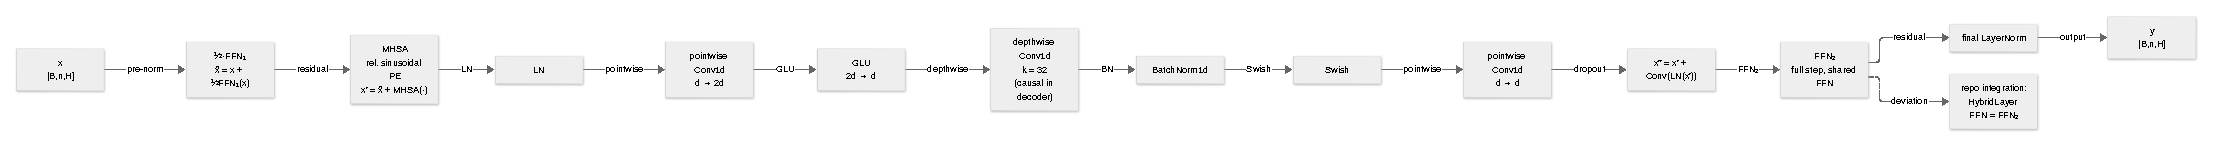
\includegraphics{../paper/figures/mixers/conformer.pdf}}
\caption{Flujo de datos del bloque Conformer: una capa feed-forward de medio paso Macaron, atención multi-cabeza con codificación posicional sinusoidal relativa, el módulo de convolución (pointwise $\to$ GLU $\to$ depthwise $\to$ BatchNorm $\to$ Swish $\to$ pointwise) y la segunda capa feed-forward seguida de la LayerNorm final. En este conjunto de herramientas la FFN compartida de \texttt{HybridLayer} ocupa la ranura $\mathrm{FFN}_2$ con un paso residual completo (anotación punteada).}
\label{fig:mixer-conformer}
\end{figure}

\subsubsection{Formulación Matemática}

Para una entrada de bloque $x \in \mathbb{R}^{B \times n \times d}$, el bloque de referencia de la Fig.~1 de \citet{Gulati2020} es
\begin{align}
\tilde{x} &= x + \tfrac{1}{2}\,\mathrm{FFN}_1\big(\mathrm{LN}(x)\big), \label{eq:conformer-ffn1}\\
x' &= \tilde{x} + \mathrm{MHSA}\big(\mathrm{LN}(\tilde{x})\big), \label{eq:conformer-mhsa}\\
x'' &= x' + \mathrm{Conv}\big(\mathrm{LN}(x')\big), \label{eq:conformer-conv}\\
y &= \mathrm{LN}\Big(x'' + \tfrac{1}{2}\,\mathrm{FFN}_2\big(x''\big)\Big). \label{eq:conformer-ffn2}
\end{align}
Los dos términos feed-forward llevan el coeficiente de \emph{medio paso} de Macaron: cada uno aporta la mitad de una actualización residual completa, uno antes y otro después del par atención--convolución.

\paragraph{Módulo feed-forward.} Con ancho oculto $d_{ff}$,
\begin{equation}
\mathrm{FFN}(x) = W_2\,\mathrm{Dropout}\big(\mathrm{Swish}(W_1\,\mathrm{LN}(x) + b_1)\big) + b_2,
\qquad
\mathrm{Swish}(a) = a\,\sigma(a),
\label{eq:conformer-ffn}
\end{equation}
donde $W_1 \in \mathbb{R}^{d_{ff} \times d}$, $W_2 \in \mathbb{R}^{d \times d_{ff}}$ y $\sigma$ es la sigmoide logística. El paper usa $d_{ff} = 4d$.

\paragraph{Atención multi-cabeza con codificación posicional relativa.} Las consultas, claves y valores son proyecciones lineales de la entrada normalizada del bloque, $Q = \mathrm{LN}(\tilde{x})W_Q$, $K = \mathrm{LN}(\tilde{x})W_K$, $V = \mathrm{LN}(\tilde{x})W_V$, divididas en $H$ cabezas de ancho $d_h = d/H$. Siguiendo el esquema relativo de Transformer-XL \citep{Dai2019}, la puntuación de la consulta $i$ contra la clave $j$ suma una función sinusoidal del \emph{desplazamiento} $i-j$ en lugar de una posición absoluta:
\begin{equation}
e_{ij} = q_i^{\top} k_j + (q_i + v)^{\top} R_{i-j},
\qquad
A_{ij} = \operatorname{softmax}_j\!\Big(\frac{e_{ij}}{\sqrt{d_h}}\Big),
\qquad
O = A V W_O,
\label{eq:conformer-relpe}
\end{equation}
con $v$ un vector de sesgo aprendido y, para $m = 0, \dots, d_h/2 - 1$,
\begin{equation}
R_{\delta,\,2m} = \sin\!\big(\delta\,/\,10000^{2m/d_h}\big),
\qquad
R_{\delta,\,2m+1} = \cos\!\big(\delta\,/\,10000^{2m/d_h}\big).
\label{eq:conformer-sinusoid}
\end{equation}
Como la codificación depende solo de $\delta = i-j$, el bloque generaliza entre longitudes de utterance. El conjunto de herramientas canaliza la información posicional por la maquinaria de todo el modelo que usan los demás mezcladores: \texttt{model.positional\_encoding} (RoPE por defecto) se aplica a $Q/K$, y \texttt{conformer\_attn\_use\_pe} (\texttt{true} por defecto) permite que una capa lo omita. El esquema sinusoidal relativo del paper se aproxima mejor con \texttt{sinusoidal\_rotary} (frecuencias sinusoidales aplicadas como rotación sobre $Q/K$, relativo por construcción); \texttt{alibi}/\texttt{bam} aportan un sesgo de distancia en lugar de una rotación. No se implementa un módulo sinusoidal relativo dedicado estilo Transformer-XL. En modo decoder la matriz de puntuaciones recibe la máscara causal habitual antes del softmax, y se usa la ruta de softmax fijo del Anexo~\ref{sec:fixed-implementation} cuando \texttt{numerics.fixed\_softmax} está habilitado.

\paragraph{Módulo de convolución.} El módulo aplica una convolución depthwise con compuerta sobre el eje temporal:
\begin{align}
h &= \mathrm{LN}(x'), \\
[u,\, g] &= \mathrm{Conv1d}_{d \to 2d}(h), \qquad
\tilde{h} = u \odot \sigma(g), \label{eq:conformer-glu}\\
z_t &= \sum_{k=0}^{K-1} w_k\, \tilde{h}_{t + k - \lfloor K/2 \rfloor}, \label{eq:conformer-depthwise}\\
c &= \mathrm{Dropout}\Big(\mathrm{Conv1d}_{d \to d}\big(\mathrm{Swish}(\mathrm{BN}(z))\big)\Big), \label{eq:conformer-conv-out}
\end{align}
donde $\odot$ es el producto elemento a elemento (una GLU que reduce los $2d$ canales a $d$), $w \in \mathbb{R}^{K}$ es el kernel depthwise y $\mathrm{BN}$ normaliza cada canal sobre los ejes de batch y tiempo,
\begin{equation}
\mathrm{BN}(z)_{b,t,c} = \gamma_c\,\frac{z_{b,t,c} - \mu_c}{\sqrt{\sigma_c^2 + \epsilon}} + \beta_c .
\label{eq:conformer-bn}
\end{equation}
En modo decoder la suma de la Ecuación~\ref{eq:conformer-depthwise} se desplaza a $z_t = \sum_{k=0}^{K-1} w_k \tilde{h}_{t-K+1+k}$, de modo que ninguna trama futura entra en la convolución; los modos encoder y ViT conservan el padding simétrico ``same'' del paper.

\subsubsection{Pseudocódigo Algorítmico}

\begin{algorithm}[H]
\caption{Bloque Conformer (\texttt{conformer\_attn})}
\begin{algorithmic}[1]
\Require entrada de bloque $x \in \mathbb{R}^{B \times n \times d}$, kernel $K=32$, cabezas $H$, bandera Macaron, modo
\Ensure delta de bloque $\Delta$ tal que $x + \Delta$ entra en la $\mathrm{norm}_2 + \mathrm{FFN}_2$ exterior
\State $\tilde{x} \gets x + \mathrm{FFN}_1(\mathrm{LN}(x))$ \Comment{FFN$_1$ Macaron ($\tfrac12$ en el paper)}
\State $Q, K_{proj}, V \gets \mathrm{LN}(\tilde{x})W_Q,\ \mathrm{LN}(\tilde{x})W_K,\ \mathrm{LN}(\tilde{x})W_V$
\State $e_{ij} \gets q_i^{\top}k_j + (q_i + v)^{\top}R_{i-j}$ \Comment{PE sinusoidal relativa, Ec.~\ref{eq:conformer-relpe}}
\If{modo $=$ decoder}
    \State $e_{ij} \gets -\infty$ para $j > i$ \Comment{máscara causal}
\EndIf
\State $x' \gets \tilde{x} + \mathrm{softmax}(e/\sqrt{d_h})\,V\,W_O$
\State $h \gets \mathrm{LN}(x')$
\State $[u, g] \gets \mathrm{Conv1d}_{d \to 2d}(h)$; \quad $\tilde{h} \gets u \odot \sigma(g)$ \Comment{GLU}
\State $z \gets \mathrm{DepthwiseConv1d}_{K}(\tilde{h})$ \Comment{desplazamiento causal en modo decoder}
\State $c \gets \mathrm{Dropout}(\mathrm{Conv1d}_{d \to d}(\mathrm{Swish}(\mathrm{BN}(z))))$
\State $x'' \gets x' + c$
\State \Return $x''$ \Comment{\texttt{HybridLayer} añade $\mathrm{FFN}_2$ y la LN final}
\end{algorithmic}
\end{algorithm}

\subsubsection{Mapeo de Implementación y Desviaciones}

La Tabla~\ref{tab:conformer-mapping} mapea el bloque del paper sobre el conjunto de herramientas. Las desviaciones sustantivas son los dos escalados residuales y la segunda capa feed-forward: el paper conserva ambos coeficientes $\tfrac12$ de Macaron y envuelve la $\mathrm{FFN}_2$ en el bloque, mientras que \texttt{conformer\_attn} usa pasos completos y devuelve el estado tras el módulo de convolución, dejando que el \texttt{HybridLayer} exterior aplique su $\mathrm{norm}_2 + \mathrm{FFN}$ compartida (también a paso completo). La descomposición es deliberada: mantiene disponibles para la segunda FFN el enrutamiento MoE, Mixture-of-Depths, los flujos mHC/Hyperloop, AttnRes, la fusión FlashNorm, las proyecciones BitNet y el enrutamiento de optimizadores por grupo de parámetros, nada de lo cual sobreviviría a una FFN privada dentro del mezclador.

\begin{table}[H]
\centering
\small
\begin{tabularx}{0.95\linewidth}{L{3.6cm}L{4.4cm}X}
\toprule
\textbf{Componente del paper} & \textbf{Implementación en el toolkit} & \textbf{Notas} \\
\midrule
$\tfrac{1}{2}\mathrm{FFN}_1$ (pre-norm) & FFN privada dentro de \texttt{ConformerAttention}; Swish; residual a paso completo & \texttt{conformer.macaron: true} (por defecto); el coeficiente $\tfrac12$ del paper se omite; deshabilitarla deja solo atención $+$ convolución \\
MHSA, PE sinusoidal relativa & proyecciones propias $q/k/v/out$; PE de todo el modelo vía \texttt{conformer\_attn\_use\_pe} (\texttt{true} por defecto) & la sinusoidal relativa del paper $\approx$ \texttt{sinusoidal\_rotary}; sin módulo Transformer-XL dedicado (RoPE es el valor por defecto del modelo) \\
Módulo de convolución & LN $\to$ pointwise $\to$ GLU $\to$ depthwise $\to$ BN $\to$ Swish $\to$ pointwise $\to$ dropout & \texttt{conformer.kernel\_size} (32), \texttt{conformer.conv\_norm} (\texttt{batch}/\texttt{group}/\texttt{layer}) \\
$\tfrac{1}{2}\mathrm{FFN}_2$ a medio paso & $\mathrm{norm}_2 + \mathrm{FFN}$ de \texttt{HybridLayer}, paso completo & justificado por la Tabla~5 de \citet{Gulati2020}: $1.9/4.4$ vs.\ $1.9/4.5$ WER dev (ambos coeficientes omitidos) \\
LayerNorm final & norma final de \texttt{HybridLayer} & idéntica a la de cualquier otro mezclador \\
Submuestreo convolucional $4\times$ & frontend de \texttt{frankenstein\_audio} & Anexo~\ref{sec:annex-18}; texto y ViT usan sus propios embeddings \\
Dropout ($p=0.1$) & \texttt{model.dims.dropout} & global, por bloque \\
\bottomrule
\end{tabularx}
\caption{Mapeo de implementación del bloque Conformer. Las desviaciones son los escalados Macaron $\tfrac12$ omitidos, la segunda FFN (aportada por la capa exterior a paso completo) y el cableado de la codificación posicional.}
\label{tab:conformer-mapping}
\end{table}

\paragraph{Por qué la FFN a paso completo es segura.} Omitir el $\tfrac12$ de Macaron cambia la escala residual de cada rama, no la forma expresiva del bloque: la variante de paso completo es exactamente la que \citet{Gulati2020} ablacionan en su Tabla~5, donde mueve el WER dev-clean/dev-other de $1.9/4.4$ (medio paso) a $1.9/4.5$ (paso completo), es decir, una décima. El conjunto de herramientas usa pasos completos en ambas capas feed-forward; la primera permanece privada en el mezclador y la segunda es la compartida, lo que preserva la composabilidad descrita arriba.

\subsection{Ablaciones Publicadas}

La Tabla~\ref{tab:conformer-ablations} resume las ablaciones que motivan la configuración por defecto. Los valores son los reportados por \citet{Gulati2020}; el orden cualitativo es lo que codifican los valores por defecto.

\begin{table}[H]
\centering
\small
\begin{tabularx}{0.95\linewidth}{L{3.7cm}L{4.0cm}X}
\toprule
\textbf{Ablación} & \textbf{Configuraciones comparadas} & \textbf{Resultado reportado} \\
\midrule
Módulo de convolución (Tabla~3) & presente vs.\ eliminado & la mayor degradación individual del bloque al eliminarlo; la rama local es portante, no decorativa \\
Par FFN Macaron (Tabla~3) & $\tfrac{1}{2}\mathrm{FFN}_1 + \tfrac{1}{2}\mathrm{FFN}_2$ vs.\ una FFN & eliminar el par cuesta aproximadamente $0.2$ dev-clean / $0.5$ dev-other WER \\
Medio vs.\ paso completo (Tabla~5) & residuales $\tfrac{1}{2}$ vs.\ completos & $1.9/4.4$ vs.\ $1.9/4.5$ WER dev: como máximo $0.1$ punto \\
Tamaño de kernel (Tabla~7) & $K \in \{3, 7, 17, 32, 65\}$ & $K = 32$ es el mejor; kernels pequeños subajustan el contexto local, $K = 65$ añade costo sin ganancia \\
Ubicación de la convolución & tras MHSA, antes de $\mathrm{FFN}_2$ & se conserva el orden de referencia; mover la rama no lo mejora \\
\bottomrule
\end{tabularx}
\caption{Ablaciones del Conformer y los valores por defecto que justifican (\texttt{kernel\_size: 32}, \texttt{macaron: true}, $\mathrm{FFN}_2$ compartida a paso completo).}
\label{tab:conformer-ablations}
\end{table}

\subsection{Reutilización de la Infraestructura Existente}

Como \texttt{ConformerAttention} devuelve un delta y hereda el constructor \texttt{mixer(config, pos\_encoder=...)}, toda la pila se reutiliza sin casos especiales:

\begin{itemize}[leftmargin=*]
    \item \textbf{Clases de modelo:} encoder de texto (\texttt{mlm}/\texttt{sbert}/\texttt{text\_classification}), decoder causal (\texttt{causal\_lm}), Vision Transformer (\texttt{patch\_prediction}/\texttt{classification}/\texttt{segmentation}) y \texttt{frankenstein\_audio} (\texttt{asr}, \texttt{audio\_classification}).
    \item \textbf{Normalización:} las 6 variantes, incluida pRMSNorm y la fusión FlashNorm en $\mathrm{norm}_1$/$\mathrm{norm}_2$; el módulo de convolución conserva su BatchNorm salvo que \texttt{conformer.conv\_norm} seleccione group o layer normalization.
    \item \textbf{Enrutamiento y residuales:} MoE, Mixture-of-Depths, mHC, Hyperloop, AttnRes y las proyecciones ternarias BitNet (la FFN privada y las proyecciones de la convolución son compatibles con BitLinear).
    \item \textbf{Optimizadores:} las 23 familias con prefijos por grupo; los parámetros del mezclador, incluido el kernel depthwise y las normas de la convolución, se enrutan al grupo \texttt{attention}.
    \item \textbf{Caché KV:} \texttt{conformer\_attn} se registra como \emph{no} cacheable (\texttt{supported=False}), porque el estado de la convolución depthwise y las estadísticas de BatchNorm deberían acarrearse entre pasos. \texttt{generate()} cae a la ruta de recómputo completo, que es exacta.
\end{itemize}

\subsection{Cuándo Usarlo}

\begin{itemize}[leftmargin=*]
    \item \textbf{Voz:} mezclador por defecto para \texttt{asr} y \texttt{audio\_classification}; con tramas de 40\,ms tras el submuestreo $4\times$, el kernel de 32 abarca $\sim$1.28\,s de contexto, aproximadamente el ancho de una secuencia de fonos.
    \item \textbf{Texto y visión:} sustituto sólido de \texttt{standard\_attn} cuando los datos tienen estructura local (modelos a nivel de carácter, código, OCR, secuencias de parches); cuesta una convolución depthwise y dos normas extra por capa frente a un bloque de atención plano.
    \item \textbf{Decodificación en streaming:} usable en \texttt{mode: decoder} con padding convolucional causal, pero sin la caché incremental del Anexo~\ref{sec:annex-kv-cache}; la recurrencia depthwise es la pieza que falta.
\end{itemize}

\section{Audio: Reconocimiento de Voz y Clasificación de Audio}
\label{sec:annex-18}

\subsection{Resumen Ejecutivo}

\texttt{frankenstein\_audio} es la cuarta clase de modelo del conjunto de herramientas. Posee un frontend de audio---bancos de filtros log-mel o un espectrograma crudo, SpecAugment opcional \citep{Park2019} y dos convoluciones con stride 2 que reducen la tasa de tramas $4\times$---y luego ejecuta la misma pila de \texttt{HybridLayer} que el encoder de texto sobre la secuencia de tramas resultante. Como la pila es agnóstica de modalidad, todos los mezcladores de secuencia (incluido el Conformer del Anexo~\ref{sec:annex-17}), normas, estrategias de residual, codificaciones posicionales, optimizadores y bloques de enrutamiento están disponibles sin cambios. La clase soporta dos tareas: \textbf{reconocimiento automático de voz} (\texttt{asr}, con pérdida CTC \citep{Graves2006ctc} o RNN-Transducer \citep{Graves2012}) y \textbf{clasificación de audio} (\texttt{audio\_classification}, entropía cruzada a nivel de clip). El mismo frontend, con \texttt{audio.feature: raw}, acepta señales de sensores multicanales unidimensionales como EEG, EMG o acelerómetro para clasificación.

La receta de referencia es el frontend Conformer de \citet{Gulati2020}: bancos de filtros log-mel de 80 canales con ventana de 25\,ms y salto de 10\,ms, dos convoluciones $3\times3$ con stride 2, una proyección lineal al ancho del modelo y SpecAugment con ancho de frecuencia $F=27$, diez máscaras temporales y una razón máxima de máscara temporal $p_S = 0.05$. Los tres tamaños de referencia (S/M/L) se reproducen en la Tabla~\ref{tab:audio-sizes}.

\subsection{La Clase de Modelo \texttt{frankenstein\_audio}}

\begin{figure}[H]
\centering
\fitfigure{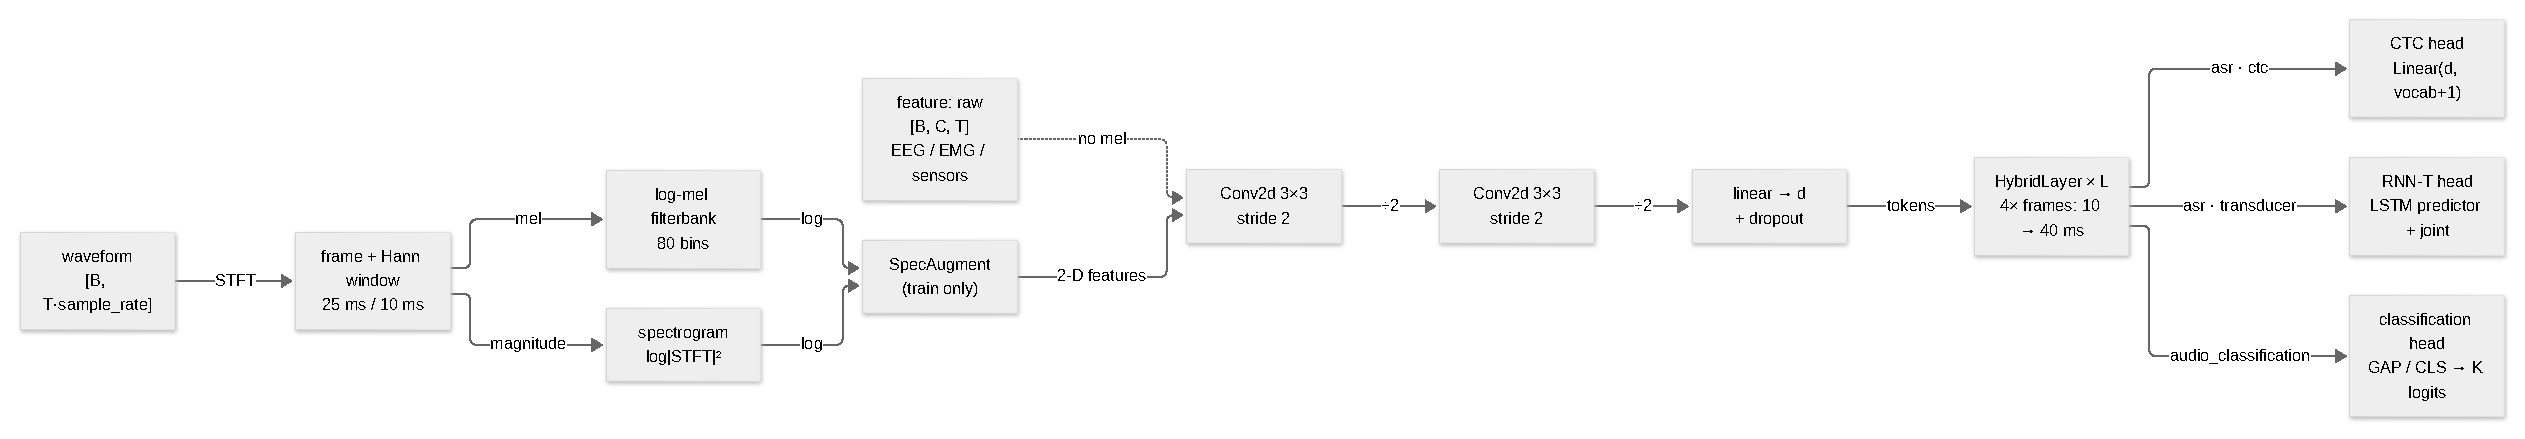
\includegraphics{../paper/figures/audio_frontend.pdf}}
\caption{Flujo de datos del frontend de audio: waveform $\to$ enmarcado 25\,ms/10\,ms $\to$ log-mel de 80 bins (o espectrograma, o tramas multicanal crudas) $\to$ SpecAugment (solo entrenamiento) $\to$ dos etapas Conv2d con stride 2 ($4\times$) $\to$ proyección lineal $\to$ pila \texttt{HybridLayer} $\to$ cabeza CTC, RNN-T o de clasificación.}
\label{fig:audio-frontend}
\end{figure}

\subsubsection{Frontend de Audio}

El módulo frontend convierte un lote de formas de onda $w \in \mathbb{R}^{B \times T}$ (o un lote de clips multicanal $w \in \mathbb{R}^{B \times C \times T}$ en modo \texttt{raw}) en un mapa de características:

\begin{enumerate}[leftmargin=*]
    \item \textbf{Enmarcado:} la forma de onda se corta en ventanas solapadas de \texttt{window\_ms} $=25$\,ms cada \texttt{stride\_ms} $=10$\,ms, con ventana de Hann, a \texttt{sample\_rate} $=16000$\,Hz. A la tasa de referencia esto produce tramas de 400 muestras con salto de 160, es decir, 100 tramas por segundo.
    \item \textbf{Representación espectral} (\texttt{audio.feature}):
    \begin{itemize}[leftmargin=*]
        \item \texttt{logmel} (por defecto): banco de filtros mel de $80$ bins (Ecuación~\ref{eq:audio-mel}) seguido de compresión logarítmica;
        \item \texttt{spectrogram}: $\log|\mathrm{STFT}(w)|^2$ sin proyección mel;
        \item \texttt{raw}: sin transformada espectral; el clip se entrega como mapa $C \times T$ (Sección~\ref{sec:annex-18-eeg}).
    \end{itemize}
    \item \textbf{SpecAugment} \citep{Park2019}: se enmascaran $F$ canales de frecuencia por clip y hasta \texttt{time\_masks} bandas temporales de ancho máximo $p_S \cdot T$, ambas con relleno de ceros (solo entrenamiento).
\end{enumerate}

El banco de filtros mel es
\begin{equation}
M_k(f) = \max\Big(0,\ \min\Big(\tfrac{f-f_{k-1}}{f_k-f_{k-1}},\ \tfrac{f_{k+1}-f}{f_{k+1}-f_k}\Big)\Big),
\label{eq:audio-filterbank}
\end{equation}
para $K = 80$ filtros triangulares espaciados en la escala mel, $\mathrm{mel}(f) = 2595 \log_{10}(1 + f/700)$, y la característica log-mel es
\begin{equation}
x_k = \log\Big(\sum_{f} M_k(f)\,|X(f)|^2 + \epsilon\Big).
\label{eq:audio-mel}
\end{equation}
Cuando \texttt{torchaudio} es importable, el frontend usa \texttt{torchaudio.transforms.MelSpectrogram} para la Ecuación~\ref{eq:audio-mel}; en caso contrario recurre a una implementación en PyTorch puro construida sobre \texttt{torch.stft} y una matriz de filtros en caché. Ambas rutas son numéricamente equivalentes salvo la convención del banco de filtros (espaciado mel HTK vs.\ Slaney), y la ruta en PyTorch puro es la que mantiene la CI solo-CPU libre del extra opcional \texttt{audio}.

\subsubsection{Submuestreo Convolucional}

Dos etapas convolucionales reducen la tasa de tramas $4\times$ (10\,ms $\to$ 40\,ms), que es lo que convierte un utterance de 30 segundos en una secuencia de $\sim$750 tokens en lugar de 3000:
\begin{equation}
F = \mathrm{Dropout}\Big(W_p\,\mathrm{Conv2d}_{3\times3,\,s=2}\big(\mathrm{Conv2d}_{3\times3,\,s=2}(X)\big)\Big),
\qquad W_p \in \mathbb{R}^{d \times d_c},
\label{eq:audio-subsampling}
\end{equation}
donde $X$ es el mapa de características $\texttt{n\_mels} \times T'$ con \texttt{conv\_channels} canales tras la primera etapa, y $W_p$ proyecta los canales aplanados al ancho del modelo $d$. Ambas etapas son fijas, con kernels $3\times3$ y stride 2; \texttt{audio.conv\_channels} (32) fija el ancho de canales de la primera etapa y \texttt{audio.n\_fft} (400) el tamaño de la STFT.

\subsubsection{Modo Encoder Forzado y la Pila HybridLayer}

\texttt{frankenstein\_audio} fuerza \texttt{mode: encoder}, exactamente como \texttt{frankenstein\_vit}: las tareas de audio son bidireccionales (un encoder CTC o transducer debe ver tramas pasadas y futuras), y el padding convolucional del Conformer es simétrico en modo encoder. La clase refleja el patrón envoltorio del ViT---frontend, pila de \texttt{HybridLayer}, cabeza de tarea---y su bucle de capas conserva los mismos hooks, de modo que AttnRes, mHC, Hyperloop, profundidad en bucle, MoE, Mixture-of-Depths y BitNet funcionan sin código específico de audio. Las cabezas de tarea se construyen tras la normalización final:

\begin{itemize}[leftmargin=*]
    \item \textbf{CTC:} $\mathrm{Linear}(d, V+1)$ sobre la secuencia de tramas, donde la clase extra es el blank.
    \item \textbf{RNN-T:} una red de predicción LSTM de una capa sobre las etiquetas no-blank previas (\texttt{audio.asr\_decoder\_dim}, \texttt{asr\_decoder\_layers}, \texttt{asr\_decoder\_dropout}), y una red conjunta $z_{t,u} = \tanh(W_e h_t + W_p h_u + b)$, $\mathrm{logits}_{t,u} = W_o z_{t,u}$.
    \item \textbf{Clasificación:} un vector agrupado (global average pooling, o un token \texttt{[CLS]} aprendido antepuesto a la secuencia de tramas, según \texttt{pooling\_mode}) proyectado a \texttt{num\_classes} logits.
\end{itemize}

\subsection{Reconocimiento Automático de Voz}

\subsubsection{CTC}

La clasificación temporal conexionista \citep{Graves2006ctc} marginaliza sobre todas las alineaciones a nivel de trama que colapsan a la secuencia objetivo $y$ bajo el mapa muchos-a-uno $\mathcal{B}$ (fusionar repeticiones, borrar blanks):
\begin{equation}
\mathcal{L}_{\text{CTC}} = -\log \sum_{\pi \in \mathcal{B}^{-1}(y)} \prod_{t=1}^{T} p(\pi_t \mid x),
\label{eq:audio-ctc}
\end{equation}
calculada con la implementación \texttt{ctc\_loss} de \texttt{torch.nn.functional} en espacio logarítmico con \texttt{zero\_infinity=False}, para que las alineaciones imposibles no envenenen el gradiente.

\subsubsection{RNN-Transducer}

La pérdida RNN-T \citep{Graves2012} suma sobre alineaciones de \emph{etiqueta-y-blank} en la retícula $T \times (U+1)$. Con $\alpha_{t,u}$ la log-probabilidad del prefijo $y_{1:u}$ tras $t$ tramas de encoder, la recursión forward es
\begin{equation}
\alpha_{t,u} = \operatorname{logsumexp}\Big(
\underbrace{\alpha_{t-1,u} + \log p(\varnothing \mid t-1, u)}_{\text{avanzar tiempo}},
\;
\underbrace{\alpha_{t,u-1} + \log p(y_u \mid t, u-1)}_{\text{emitir etiqueta}}
\Big),
\label{eq:audio-rnnt}
\end{equation}
con $\alpha_{0,0} = 0$ y $-\infty$ en el resto, $p(\cdot \mid t,u) = \operatorname{softmax}(\mathrm{logits}_{t,u})$, y
\begin{equation}
\mathcal{L}_{\text{RNN-T}} = -\alpha_{T,U}.
\label{eq:audio-rnnt-loss}
\end{equation} La implementación es compatible con autograd en PyTorch puro (programación dinámica en dominio logarítmico sobre la retícula, con el gradiente obtenido por la recursión backward estándar), y toma la ruta rápida \texttt{torchaudio.functional.rnnt\_loss} cuando la dependencia opcional está instalada. La retícula es $O(T \cdot U)$ en memoria, por lo que el predictor se mantiene superficial (\texttt{audio.asr\_decoder\_layers}, por defecto 1) y estrecho (\texttt{audio.asr\_decoder\_dim}, 320 por defecto). La pérdida se selecciona con \texttt{audio.asr\_loss} (\texttt{ctc} por defecto).

\subsubsection{Decodificación y Tasa de Error}

La decodificación CTC voraz toma el argmax por trama, colapsa repeticiones y elimina blanks. La decodificación RNN-T voraz alterna una emisión de etiqueta con un avance de trama hasta que el blank puntúa más alto que la siguiente etiqueta. Ambas se evalúan con la tasa de error de caracteres
\begin{equation}
\mathrm{CER} = \frac{S + D + I}{N},
\label{eq:audio-cer}
\end{equation}
donde $S$, $D$, $I$ son las sustituciones, deleciones e inserciones del alineamiento de Levenshtein contra la transcripción de referencia y $N$ es la longitud de referencia.

\subsection{Clasificación de Audio}

La clasificación reutiliza las convenciones de pooling y cabeza del Vision Transformer (Anexo~\ref{sec:annex-vision}): \texttt{pooling\_mode: cls} antepone un token aprendido y lee la posición 0, \texttt{pooling\_mode: gap} (el valor por defecto) promedia las salidas de las tramas. La cabeza es un $\mathrm{Linear}(d, K)$ inicializado en cero, entrenado con entropía cruzada y el mismo control de suavizado de etiquetas que las tareas de visión. SpecAugment se aplica al mapa de características antes del submuestreo, de modo que aumenta la entrada, nunca la secuencia de tokens.

\subsection{SpecAugment}

Siguiendo a \citet{Park2019} en su configuración ``LibriSpeech basic'', los dos tipos de máscara se aplican de forma independiente por clip:
\begin{equation}
\Delta f \sim \mathcal{U}[0, F], \quad f_0 \sim \mathcal{U}[0, \nu - \Delta f],
\qquad
\Delta t \sim \mathcal{U}[0, p_S \cdot T], \quad t_0 \sim \mathcal{U}[0, T - \Delta t],
\label{eq:audio-specaugment}
\end{equation}
con $F = 27$, \texttt{time\_masks} $= 10$ y $p_S = 0.05$, cada máscara poniendo a cero un rectángulo $\Delta f \times \Delta t$. La \emph{deformación temporal} (time warping), la tercera transformación de SpecAugment, no está implementada: requiere una deformación del eje temporal por muestra que interactúa mal con el bucketing de longitud fija del dataset. El enmascaramiento de frecuencia y de tiempo concentran la mayor parte del beneficio de regularización en las propias ablaciones del paper, y ambos se desactivan en evaluación.

\subsection{Tamaños de Referencia}

\begin{table}[H]
\centering
\small
\begin{tabular}{L{2.3cm}cccccc}
\toprule
\textbf{Variante} & \textbf{Capas} & \textbf{$d$} & \textbf{Cabezas} & \textbf{Kernel} & \textbf{Paráms.} & \textbf{RNN-T $d_{dec}$} \\
\midrule
Conformer-S & 16 & 144 & 4 & 32 & 10.3M & 320 \\
Conformer-M & 17 & 256 & 4 & 32 & 30.7M & 640 \\
Conformer-L & 17 & 512 & 8 & 32 & 118.8M & 640 \\
\bottomrule
\end{tabular}
\caption{Tamaños de referencia del Conformer de \citet{Gulati2020} (Tabla~1), que siguen los presets de ejemplo. El ancho del decoder RNN-T solo se usa cuando \texttt{audio.asr\_loss: transducer}.}
\label{tab:audio-sizes}
\end{table}

\subsection{Configuraciones de Ejemplo}

Los ejemplos de ASR usan \texttt{astroza/chilean-jokes-festival-de-vina} (audio en español a 16\,kHz con transcripciones, 50 filas), un dataset lo bastante pequeño para ejecutarse de extremo a extremo en CPU como prueba de humo. El ejemplo de clasificación recurre al \texttt{DummyAudioDataset} sintético cuando no hay dataset accesible.

\begin{verbatim}
model_class: frankenstein_audio
model:
  dims: {hidden_size: 144, num_layers: 16, num_heads: 4}
  dims.layer_pattern: [conformer_attn, ...]   # 16 entradas
  attention.conformer: {kernel_size: 32, macaron: true, conv_norm: batch}
audio:
  feature: logmel
  sample_rate: 16000
  n_mels: 80
  window_ms: 25
  stride_ms: 10
  n_fft: 400
  conv_channels: 32
  asr_loss: ctc          # o transducer
  asr_decoder_dim: 320
  asr_decoder_layers: 1
  asr_decoder_dropout: 0.1
audio_dataset:
  dataset_name: astroza/chilean-jokes-festival-de-vina
  split: train
  audio_column: audio
  text_column: text
  spec_augment: {enabled: true, freq_mask_width: 27,
                 time_masks: 10, time_mask_ratio: 0.05}
training:
  task: asr
\end{verbatim}

\subsection{Señales 1-D Genéricas: EEG y Más Allá}
\label{sec:annex-18-eeg}

El frontend no está atado a la voz. Con \texttt{audio.feature: raw}, el banco de filtros mel y SpecAugment se omiten y el clip se trata como un mapa multicanal $C \times T$, con \texttt{audio.in\_channels: C}. Las dos convoluciones con stride 2 actúan entonces como un banco de filtros aprendido sobre el tiempo (y, como efecto secundario, sobre el eje de canales), la proyección lineal produce tokens de ancho $d$, y la pila de \texttt{HybridLayer} ve una secuencia de tramas exactamente como en voz. Esto hace usable la clase, al menos para \textbf{clasificación}, en:

\begin{itemize}[leftmargin=*]
    \item \textbf{EEG:} $C$ electrodos $\times$ $T$ muestras por época, etiquetadas con un estado cognitivo, fase de sueño o patología; los electrodos juegan el papel de los canales mel.
    \item \textbf{EMG / ECG / EDA:} uno o pocos canales, etiquetados con gesto, actividad o clase de anomalía.
    \item \textbf{Acelerómetro / IMU:} $C \in \{3, 6, 9\}$ ejes, etiquetados con actividad o estado del dispositivo.
    \item \textbf{Sensores industriales y ambientales:} trazas de vibración, presión o emisión acústica, etiquetadas por ventana.
\end{itemize}

\paragraph{Qué se conserva.} Todo lo que está aguas abajo del frontend: los 45 mezcladores (Conformer es un buen valor por defecto porque su rama de convolución coincide con la morfología local de las bioseñales), las 6 normas, AttnRes/mHC/MoE/MoD, los 23 optimizadores, la receta de encoder congelado de \texttt{text\_classification} y las rutas de checkpoint y despliegue. El bucketing por longitud, las máscaras de padding y la evaluación tipo CER son del lado del dataset y no dependen de la modalidad.

\paragraph{Limitaciones.} El modo raw es una comodidad, no un reemplazo de un frontend de dominio:
\begin{enumerate}[leftmargin=*]
    \item \textbf{Submuestreo del eje de canales.} Las dos etapas \texttt{Conv2d} con stride 2 son fijas y reducen a la mitad ambos ejes espaciales, así que un montaje con menos de cuatro canales pierde su eje de canales por completo; mantenga $C \geq 4$ (o proyecte el montaje a un mapa más ancho primero).
    \item \textbf{Sin geometría del montaje.} Las posiciones de los electrodos, los montajes referenciales vs.\ bipolares y las correlaciones inter-canal no se codifican; la convolución ve los canales como una pila sin orden, a diferencia de los modelos específicos de EEG con priors topográficos o de grafo.
    \item \textbf{Sin prior espectral.} \texttt{logmel} y \texttt{spectrogram} asumen límites de banda y espaciado mel que no aplican por debajo de 20\,Hz ni por encima de 8\,kHz; el modo raw evita el desajuste pero también pierde el sesgo inductivo alineado a la banda.
    \item \textbf{Solo clasificación.} CTC y RNN-T requieren una secuencia objetivo a nivel de token. El etiquetado secuencia-a-secuencia de ventanas de sensores (p.\,ej.\ secuencias de fases de sueño) queda fuera de alcance; use clasificación por ventana y un decodificador posterior.
    \item \textbf{Estadísticas y normalización.} La BatchNorm del módulo de convolución usa estadísticas por lote; en EEG la escala de amplitud varía por sujeto y sesión, por lo que se recomienda normalizar por canal en el dataset en lugar de confiar en el frontend.
    \item \textbf{Supuestos de tasa de muestreo.} \texttt{sample\_rate} se usa para convertir \texttt{window\_ms}/\texttt{stride\_ms} en muestras; para señales crudas ajústelo a la tasa real de adquisición y elija la ventana en milisegundos en consecuencia.
\end{enumerate}

\subsection{Pseudocódigo en PyTorch}

\begin{algorithmic}[1]
\State \textbf{Entrada:} formas de onda $w$, longitudes $\ell$, transcripciones $y$ (ASR) o etiquetas $c$ (clasificación)
\State $F \gets \texttt{frontend}(w)$ \Comment{log-mel / espectrograma / raw, $(B, C, 80, T')$}
\State $F \gets \texttt{spec\_augment}(F)$ \Comment{solo entrenamiento}
\State $F \gets \texttt{conv2d}_{3\times3, s=2}(F)$; \quad $F \gets \texttt{conv2d}_{3\times3, s=2}(F)$
\State $x \gets \texttt{dropout}(\texttt{linear}(F))$ \Comment{tokens $(B, T'/4, d)$}
\State $x \gets x + \texttt{pos\_encoder}(x)$ \Comment{posiciones de trama, no bins mel}
\For{cada \texttt{layer} en \texttt{layers}}
    \State $x \gets \texttt{layer}(x)$ \Comment{\texttt{HybridLayer}, modo encoder forzado}
\EndFor
\State $x \gets \texttt{final\_norm}(x)$
\If{tarea $=$ asr y pérdida $=$ ctc}
    \State $\mathrm{logits} \gets \texttt{ctc\_head}(x)$; \quad $\mathcal{L} \gets \texttt{ctc\_loss}(\log\mathrm{softmax}(\mathrm{logits}), y, \ell/4)$
\ElsIf{tarea $=$ asr y pérdida $=$ transducer}
    \State $h^{pred} \gets \texttt{predictor}(y)$; \quad $\mathrm{logits}_{t,u} \gets \texttt{joint}(x_t, h^{pred}_u)$
    \State $\mathcal{L} \gets \texttt{rnnt\_loss}(\mathrm{logits}, y, \ell/4)$
\Else
    \State $\mathrm{logits} \gets \texttt{class\_head}(\texttt{pool}(x))$; \quad $\mathcal{L} \gets \mathrm{CE}(\mathrm{logits}, c)$
\EndIf
\end{algorithmic}

\subsection{Desviaciones y Notas de Implementación}

\begin{itemize}[leftmargin=*]
    \item \textbf{torchaudio opcional.} El frontend prefiere \texttt{torchaudio.transforms} pero nunca lo requiere; la alternativa en PyTorch puro mantiene la CI solo-CPU y el extra \texttt{cpu} libres de torchaudio (decisión D7 de la guía de arquitectura).
    \item \textbf{Deformación temporal.} No implementada (la Ecuación~\ref{eq:audio-specaugment} cubre solo enmascaramiento de frecuencia y tiempo); es la transformación que el paper usa menos.
    \item \textbf{Predictor superficial.} La red de predicción RNN-T es una sola capa LSTM por defecto (\texttt{audio.asr\_decoder\_layers}), cambiando el predictor más profundo del paper por una retícula $O(T \cdot U)$ que cabe en memoria con los tamaños de lote de referencia.
    \item \textbf{Exportación.} Las exportaciones a HuggingFace y GGUF rechazan explícitamente los artefactos de audio, como hacen con SBERT: no existe un mapeo upstream \texttt{FrankensteinForAudioClassification}. \texttt{deploy --format standard|quantized} funciona sin cambios.
    \item \textbf{Caché.} No hay caché de encoder incremental para audio; ASR consume un utterance completo por forward.
\end{itemize}


\end{document}
